\documentclass[12pt]{uthesis-v12}  %---> DO NOT ALTER THIS COMMAND
\usepackage{adjustbox}
\usepackage{booktabs}
\makeatletter
\let\latex@xfloat=\@xfloat
\def\@xfloat #1[#2]{%
    \latex@xfloat #1[#2]%
    \def\baselinestretch{1}
    \@normalsize\normalsize
    \normalsize
}
\makeatother
\usepackage{amsmath}
\usepackage{mathtools}
\usepackage{epigraph}
\usepackage{cancel}
\usepackage{xcolor}
\newcommand\Ccancel[2][black]{\renewcommand\CancelColor{\color{#1}}\cancel{#2}}
\usepackage{algorithm}
\usepackage{graphicx}
\usepackage[noend]{algpseudocode}
\usepackage{gnuplot-lua-tikz}
\usepackage[utf8]{inputenc}
\usepackage{pgfplots}
\usepackage{tabularx}
\DeclareUnicodeCharacter{2212}{−}
\usepgfplotslibrary{groupplots,dateplot}
\usetikzlibrary{patterns,shapes.arrows}
\pgfplotsset{compat=newest}
\begin{document} %---> %---> %---> %---> DO NOT ALTER THIS COMMAND

%--------+----------------------------------------------------------+
%        |  \title{}                                    (REQUIRED)  |
%        |  \author{}                                   (REQUIRED)  |
%        |                                                          |
%        |  See section 3.1 of "Read_Me_First_(v12).pdf"            |
%        |                                                          |
%        |  Also see section 2.2 of above "Read Me" file for the    |
%        |  proper use of the invisible tilde ("~") character when  |
%        |  entering a middle initial in the \author command.       |
%        +----------------------------------------------------------+

\title{ Verification and Validation Method for 
\protect\\an Acoustic Mode Prediction Code for Turbomachinery Noise}

\author{Jeffrey Severino} 
%--------+----------------------------------------------------------+
%        |  \copyrightpage{}                            (REQUIRED)  |
%        |                                                          |
%        |  See section 3.2 of "Read_Me_First_(v12).pdf"            |
%        |                                                          |
%        |  1) You must enter either "yes" or "no" in this          |
%        |      command.  Inputting "yes" produces a copyright      |
%        |      notification page as the second page and inputting  |
%        |      "no" produces a blank second page.                  |
%        |  2) Input to this command is case sensitive.             |
%        |  3) Default: the "yes" option.                           |
%        +----------------------------------------------------------+

\copyrightpage{yes}

%--------+----------------------------------------------------------+
%        |  \mydocument{}                               (REQUIRED)  |
%        |                                                          |
%        |  See section 3.3 of "Read_Me_First_(v12).pdf"            |
%        |                                                          |
%        |  1) Input to this command is limited to the following    |
%        |     three options: a) Dissertation                       |
%        |                    b) Thesis                             |
%        |                    c) Project                            |
%        |  2) Input to this command is case-sensitive.             |
%        +----------------------------------------------------------+

\mydocument{Thesis}

%--------+----------------------------------------------------------+
%        |  \degree{}{}                                 (REQUIRED)  |
%        |                                                          |
%        |  See section 3.4 of "Read_Me_First_(v12).pdf"            |
%        |                                                          |
%        |  You need to provide two distinct inputs into this       |
%        |  command:                                                |
%        |     1) In the first set of braces you need to specify    |
%        |        the *exact* degree you will receive. Some         |
%        |        examples are: -) Masters of Arts                  |
%        |                      -) Masters of Science               |
%        |                      -) Doctor of Philosophy             |
%        |     2) In the second set of braces you need to state the |
%        |        *specific* discipline or area for that degree     |
%        |        (e.g., Economics, Education, Engineering, etc.).  |
%        |  Students should consult their advisor if they have any  |
%        |  questions about this information.                       |
%        +----------------------------------------------------------+

\degree{Masters of Science}{Mechanical Engineering}

%--------+----------------------------------------------------------+
%        |  \conferraldate{}{}                          (REQUIRED)  |
%        |                                                          |
%        |  See section 3.5 of "Read_Me_First_(v12).pdf"            |
%        |                                                          |
%        |  In the two set of braces enter the month and then the   |
%        |  year your degree will be *conferred* by the university. |
%        +----------------------------------------------------------+

\conferraldate{-}{2022}

%--------+----------------------------------------------------------+
%        |  \advisor{}                                  (REQUIRED)  |
%        |                                                          |
%        |  See section 3.6.2 of "Read_Me_First_(v12).pdf"          |
%        |                                                          |
%        |  1) Also see section 2.2 of "Read_Me_First_(v12).pdf"    |
%        |     for the proper use of the invisible tilde ("~")      |
%        |     character when entering a middle initial or the      |
%        |     abbreviation of an academic title (e.g., Dr.) in     |
%        |     the \advisor{} command.                              |
%        |  2) Also see section 3.6.1. for consistent presentation  |
%        |     of title page signature lines.                       |
%        +----------------------------------------------------------+

\advisor{Dr.~Ray Hixon}

%--------+----------------------------------------------------------+
%        |  Committee Member Signature Commands         (OPTIONAL)  |
%        |                                                          |
%        |  See section 3.6.3 of "Read_Me_First_(v12).pdf"          |
%        |                                                          |
%        |  1) Use the commands below to provide signature lines    |
%        |     for your "other" committee members;                  |
%        |        --> you must list your other committee members    |
%        |            in alphabetic order by last name              |
%        |        --> to do this, use the commands below in the     |
%        |            order presented below.                        |
%        |  2) You can choose to include none, some, or all of the  |
%        |     "XXXmember" commands below --- based on the number   |
%        |     committee members you have; simply delete (or        |
%        |     comment-out) any of the commands below that are not  |
%        |     needed.                                              |
%        |  3) Do not include the name of your committee chair or   |
%        |     the Graduate Dean in the commands listed below.      |
%        |     Their signature lines are generated by the           |
%        |     \advisor{} and \graduatedean{}{} commands.           |
%        |  4) You cannot use any of the commands below more than   |
%        |     once. (For details on this issue, see section 3.6.3  |
%        |     of "Read_Me_First_(v12).pdf".)                       |
%        |  5) Also see section 2.2 of "Read_Me_First_(v12).pdf"    |
%        |     for the proper use of the invisible tilde ("~")      |
%        |     character when entering a middle initial or the      |
%        |     abbreviation of an academic title (e.g., Dr.) in     |
%        |     the commands below.                                  |
%        |  6) See section 3.6.1. for consistent presentation of    |
%        |     title page signature lines.                          |
%        |                                                          |
%        |  I know I shouldn't have to say this, but enough         |
%        |  students over the years have made the same mistake      |
%        |  that I'm forced to state:                               |
%        |                                                          |
%        |      THE NAMES USED IN THE FOLLOWING COMMANDS ARE        |
%        |      SILLY NAMES I'VE USED AS EXAMPLES ONLY.  THEY       |
%        |      ARE NOT THE ACTUAL NAMES OF YOUR COMMITTEE          |
%        |      MEMBERS.  REPLACE THE SILLY NAMES BELOW WITH        |
%        |      THE NAMES OF YOUR ACTUAL COMMITTEE MEMBERS.         |
%        |                                                          |
%        +----------------------------------------------------------+

  \secondmember{Dr.~Chinhua Sheng}
  \thirdmember{Dr.~Soric Cioc}
%  \fourthmember{Dr.~Adam Baum}
%   \fifthmember{Dr.~Corey O.~Graff}
%   \sixthmember{Dr.~Hugh Jass}
% \seventhmember{Dr.~Noah Lott}
%  \eighthmember{Dr.~Jean Poole}
%
%--------+----------------------------------------------------------+
%        |  \graduatedean{}{}                           (REQUIRED)  |
%        |                                                          |
%        |  See section 3.6.4 of "Read_Me_First_(v12).pdf"          |
%        |                                                          |
%        |  1) THE NAME AND TITLE PROVIDED BELOW ARE THOSE OF THE   |
%        |     ACTUAL GRADUATE DEAN AT THE TIME THIS DOCUMENT WAS   |
%        |     CONSTRUCTED (January 2012). Contact the Graduate     |
%        |     College to determine whether this information is     |
%        |     correct at the time you submit your document.        |
%        |  2) Section 2.2 of "Read_Me_First_(v12).pdf" describes   |
%        |     the proper use of the invisible tilde ("~")          |
%        |     character when entering a middle initial or the      |
%        |     abbreviation of an academic title (e.g., Dr.) in     |
%        |     the \graduatedean{} command.                         |
%        |  3) See section 3.6.1. for consistent presentation of    |
%        |     title page signature lines.                          |
%        +----------------------------------------------------------+

\graduatedean{Dr.~Patricia R.~Komuniecki}{Dean}

%--------+----------------------------------------------------------+
%        |  \maketitle                                  (REQUIRED)  |
%        |                                                          |
%        |  See section 3.7 of "Read_Me_First_(v12).pdf"            |
%        |                                                          |
%        |  This is a required LaTeX command; to be brief, bad      |
%        |  things will happen if this command is not included      |
%        |  in your document at this particular location.           |
%        +----------------------------------------------------------+

\maketitle  %---->  ----->  ---->  ---->   DO NOT ALTER THIS COMMAND

%--------+----------------------------------------------------------+
%        |  Abstract Page Environment                   (REQUIRED)  |
%        |                                                          |
%        |  See section 3.8 of "Read_Me_First_(v12).pdf"            |
%        +----------------------------------------------------------+

\begin{abstractpage}
Over the last 20 years, there has been an increase in computational fluid dynamic 
codes that have made numerical analysis more and more readily available, allowing
turbomachine designers to create more novel designs. However, as airport noise
limitations become more restrictive over time, reducing aircraft 
takeoff and landing noise remains a prominent issue in the aviation community. 
One popular method to reduce aircraft noise is using acoustic liners placed on 
the walls of the engine inlet and exhaust ducts. These liners are designed to 
reduce the amplitude of acoustic modes emanating from the bypass fan as they 
propagate through the engine. The SWIRL code is a frequency-domain linearized 
Euler equation solver that is designed to predict the effect of acoustic liners
on acoustic modes propagating in realistic sheared and swirling mean flows, guiding
the design of more efficient liner configurations. The purpose of this study is
to validate SWIRL using the Method Of Manufactured Solutions (MMS). This study 
also investigated the effect of the integration and spatial differencing methods 
on the convergence for a given Manufactured Solution. In addition, the effect 
of boundary condition implementation was tested.  The improved MMS convergence
rates shown for these tests suggest that the revised SWIRL code provides more 
accurate solutions with less computational effort than the original formulation.



\end{abstractpage}

%--------+----------------------------------------------------------+
%        |  Dedication Page Environment                 (OPTIONAL)  |
%        |                                                          |
%        |  See section 3.9 of "Read_Me_First_(v12).pdf"            |
%        |                                                          |
%        |  If both a dedication page and an acknowledgements page  |
%        |  are included in the document, the dedication page must  |
%        |  proceed the acknowledgements page.                      |
%        +----------------------------------------------------------+

\begin{dedication}
\noindent For my friends and family, who have always believed in my potential 
when I did not believe it myself. 
\end{dedication}

%--------+----------------------------------------------------------+
%        |  Acknowledgments Page Environment            (OPTIONAL)  |
%        |                                                          |
%        |  See section 3.10 of "Read_Me_First_(v12).pdf"           |
%        |                                                          |
%        |  If both a dedication page and an acknowledgements page  |
%        |  are included in the document, the dedication page must  |
%        |  proceed the acknowledgements page.                      |
%        +----------------------------------------------------------+

\begin{acknowledgments}
\noindent This work is supported by the NASa Advanced Air Transport Technologies
(AATT) Project. I would like to thank Edmane Envia of the NASA Glenn Research Center, who
is the technical monitor of this work. 
A very special thanks goes to Dr. Ray Hixon who supervised and guided me through
out my course work and Master's Thesis. His rigor and tenacity in his profession has 
been the model example for an aspiring aeroacoustician. 
I would like to also thank all of my committee members, Dr. Chunhua Sheng and 
Dr. Sorin Cioc. Their contributions have been instrumental. Thanks to Dr. Clifford
Brown for his programatic insights. 

I would also like to thank my focus group peers, Zaid Sabri, Matthew Gibbons ,
and Gabriel Gutierrez for their patience and support over the years. I wish them the best in all of 
their endevours.


\end{acknowledgments}

%--------+----------------------------------------------------------+
%        |  \tableofcontents                            (REQUIRED)  |
%        |  \listoftables                            (CONDITIONAL)  |
%        |  \listoffigures                           (CONDITIONAL)  |
%        |                                                          |
%        |  See sections 3.11 & 3.12 of "Read_Me_First_(v12).pdf"   |
%        |                                                          |
%        |  1) You must include the \tableofcontents command in     |
%        |     your document: the UT Manual requires every          |
%        |     dissertation/thesis to have a detailed table of      |
%        |     contents.                                            |
%        |  2) Including the \listoftables and \listoffigures       |
%        |     commands is "conditional."  See sections 3.12 of     |
%        |     "Read_Me_First_(v12).pdf" for additional details.    |
%        +----------------------------------------------------------+

\tableofcontents  %----->  ----->  ---->  DO NOT ALTER THIS COMMAND
\listoftables \listoffigures
\begin{listofsymbols}
    \emblem{$A$        }{mean flow speed of sound}
    \emblem{$A_T      $}{speed of sound at the duct radius}
    \emblem{$\tilde{A}$}{dimensionless speed of sound, $\frac{A}{A_T}$}
    \emblem{$D/Dt$     }{material derivative, $\partial/\partial t + V \cdot \nabla $}
    \emblem{$D_N$      }{derivative matrix using $N$ points}
    \emblem{$\textbf{e}_x$,$\textbf{e}_{\theta}$ }{s}
    \emblem{$k_x$      }{perturbation axial wavenumber}
    \emblem{$k$       }{reduced frequency, $\omega r_{max}/A_{T}$}
    \emblem{$m$       }{number of nodal diameters, i.e. azimuthal mode number}
    \emblem{$M_x$     }{axial Mach number}
    \emblem{$M_{\theta}$  }{tangential Mach number}
    \emblem{$P$       }{mean pressure}
    \emblem{$p'$       }{perturbation pressure}
    \emblem{$r$       }{radial coordinate}
    \emblem{$r_{min}$       }{hub radius, i.e. minimum radius}
    \emblem{$r_{max}$       }{hub radius, i.e. maximum radius}
    \emblem{$\bar{r}$      }{dimensionless radial coordinate, $r/r_{max}$}
    \emblem{$S$}{mean entropy}
    \emblem{$s'$}{perturbation entropy}
    \emblem{$t$}{time}
    \emblem{$\vec{V}$}{mean flow velocity vector}
    \emblem{$V$}{mean flow velocity}
    \emblem{$v'$}{perturbation flow velocity}
    \emblem{$V_x$}{axial component of mean flow velocity}
    \emblem{$V_{\theta}$}{tangential component of mean flow velocity}
    \emblem{$v_r'$}{axial component of perturbation velocity}
    \emblem{$v_x'$}{axial component of perturbation velocity}
    \emblem{$v_{\theta}'$}{tangential component of perturbation flow velocity}
    \emblem{$v_{\phi}$}{phase velocity,$k/\bar{\gamma}$}
    \emblem{$v_{g}$}{group velocity,$dk/d\bar{\gamma}$}
    \emblem{$x$}{axial coordinate} 

    \newpage
    \emblemskip
    \textit{Greek Symbols}
    \emblem{$\bar{\gamma}$}{dimensionless axial wavenumber, $k_x r_{max}$}
    \emblem{$\Gamma$}{free vortex strength}
    \emblem{$\bar{\Gamma}$}{$\Gamma/(r_T A_T)$}
    \emblem{$\delta$}{Kronecker delta}
    \emblem{$\eta_{H}$}{hub acoustic liner admittance (at $r_{min}$) }
    \emblem{$\eta_{T}$}{tip acoustic liner admittance (at $r_{max}$) }
    \emblem{$\Theta$}{circumferential/azimuthal coordinate}
    \emblem{$\kappa$}{ratio of specific heats}
    \emblem{$\kappa_{m\mu}$}{modal separation constant}
    \emblem{$\lambda$}{eigenvalue, $-i \bar{\gamma}$}
    \emblem{$\mu$}{radial mode index}
    \emblem{$\bar{\rho}$}{mean density}
    \emblem{$\rho'$}{perturbation density}
    \emblem{$\sigma$}{hub-to-tip radius ratio, $r_{min}/r_{max}$}
    \emblem{$\Omega$}{angular frequency for solid body swirl}
    \emblem{$\bar{\Omega}$}{$\Omega r_T/A_T$}
    \emblem{$\omega$}{perturbation angular frequency}
\end{listofsymbols}

%--------+----------------------------------------------------------+
%        |  \captionformat{}                            (REQUIRED)  |
%        |                                                          |
%        |  See section 3.12.2 of "Read_Me_First_(v12).pdf"         |
%        |                                                          |
%        |  1) You are required to choose between the "hang" or     |
%        |     "align" option for this command.                     |
%        |  2) Input to this command is case sensitive.             |
%        |  3) Default: ``hang'' option.                            |
%        +----------------------------------------------------------+

\captionformat{hang}

%--------+----------------------------------------------------------+
%        |  List of Abbreviations Environment           (OPTIONAL)  |
%        |                                                          |
%        |  See section 3.13 of "Read_Me_First_(v12).pdf"           |
%        |                                                          |
%        |  1) This is an optional section; consult your advisor    |
%        |     to determine whether you need/want to include this   |
%        |     section in your document.                            |
%        |  2) If you do not want a List of Abbreviations simply    |
%        |     delete the material below (and these instructions).  |
%        |  3) If you do want a List of Abbreviations simply        |
%        |     replace the silly material below with the            |
%        |     information relevant to your document.               |
%        |     a. Within the "listofabbreviations" environment      |
%        |        below you must use a separate \abbreviation{}{}   |
%        |        command for each entry in your List of            |
%        |        Abbreviations.                                    |
%        |     b. As the examples below demonstrate, the            |
%        |        information within the first set of braces is     |
%        |        the abbreviation and the information in the       |
%        |        second set of braces is the definition of that    |
%        |        abbreviation.                                     |
%        +----------------------------------------------------------+

\begin{listofabbreviations}

    \abbreviation{CAA}{Computational Aeroacoustics}
    \abbreviation{CFD}{Computational Fluid Dynamics}
    \abbreviation{MMS}{Method of Manufactured Solutions}
    \abbreviation{TSM}{Tanh Summation Method}
    \abbreviation{NS}{Navier-Stokes}
    \abbreviation{RK}{Runge-Kutta}

\end{listofabbreviations}

%--------+----------------------------------------------------------+
%        |  List of Symbols Environment                 (OPTIONAL)  |
%        |                                                          |
%        |  See section 3.14 of "Read_Me_First_(v12).pdf"           |
%        |                                                          |
%        |  1) This is an optional section; consult your advisor    |
%        |     to determine whether you need/want to include this   |
%        |     section in your document.                            |
%        |  2) If you do not want a List of Symbols simply delete   |
%        |     the material below (and these instructions).         |
%        |  3) If you do want a List of Symbols simply replace the  |
%        |     silly material below with the information relevant   |
%        |     to your document.                                    |
%        |       a. Within the "listofsymbols" environment below    |
%        |          you must use a separate \emblem{}{} command     |
%        |          for each entry in your List of Symbols.         |
%        |       b. As the examples below show, insert your symbol  |
%        |          within the first set of braces in the           |
%        |          \emblem{}{} command, and its definition within  |
%        |          the second set of braces.                       |
%        |       c. Use the \emblemskip command to insert a blank   |
%        |          line between different categories of symbols:   |
%        |          -) such additional spacing is required between  |
%        |             different categories of symbols;             |
%        |          -) see "Read_Me_First_(v12).pdf" for details.   |
%        +----------------------------------------------------------+

%--------+----------------------------------------------------------+
%        |  Preface Environment                         (OPTIONAL)  |
%        |                                                          |
%        |  See section 3.15 of "Read_Me_First_(v12).pdf"           |
%        +----------------------------------------------------------+

\begin{preface}
\end{preface}

%XXXXXXXXXXXXXXXXXXXXXXXXXXXXXXXXXXXXXXXXXXXXXXXXXXXXXXXXXXXXXXXXXXXX
%XXXXXXXXXXXXXXXXXXXXXXXXXXXXXXXXXXXXXXXXXXXXXXXXXXXXXXXXXXXXXXXXXXXX
%XXXXXXXXXXXXXXXXXXXXXXXXXXXXXXXXXXXXXXXXXXXXXXXXXXXXXXXXXXXXXXXXXXXX
%XXXXXXXXXXXXXXXXXXXXXXXXXXXXXXXXXXXXXXXXXXXXXXXXXXXXXXXXXXXXXXXXXXXX

%--------+----------------------------------------------------------+
%        |  \makebody                                   (REQUIRED)  |
%        |                                                          |
%        |  See section 3.16 of "Read_Me_First_(v12).pdf"           |
%        |                                                          |
%        |  This is a *required* UThesis command; again, bad        |
%        |  things will happen if this command is not included in   |
%        |  your document at this particular location --- see the   |
%        |  file "Read_Me_First_(v12).pdf" for details.             |
%        +----------------------------------------------------------+

\makebody   %------->  ------->  ------->  DO NOT ALTER THIS COMMAND

%XXXXXXXXXXXXXXXXXXXXXXXXXXXXXXXXXXXXXXXXXXXXXXXXXXXXXXXXXXXXXXXXXXXX
%XXXXXXXXXXXXXXXXXXXXXXXXXXXXXXXXXXXXXXXXXXXXXXXXXXXXXXXXXXXXXXXXXXXX
%XXXXXXXXXXXXXXXXXXXXXXXXXXXXXXXXXXXXXXXXXXXXXXXXXXXXXXXXXXXXXXXXXXXX
%XXXXXXXXXXXXXXXXXXXXXXXXXXXXXXXXXXXXXXXXXXXXXXXXXXXXXXXXXXXXXXXXXXXX

%--------+----------------------------------------------------------+
%        |  \chapter{}                                  (REQUIRED)  |
%        |                                                          |
%        |  See section 3.17 of "Read_Me_First_(v12).pdf"           |
%        |                                                          |
%        |  For guidance on using the commands \chapter{},          |
%        |  \section{}, \subsection{}, \subsubsection{}, etc., see  |
%        |  Leslie Lamport's "LaTeX: A Document Preparation         |
%        |  System." Addison Wesley: Reading Massachusetts, 1985.   |
%        +----------------------------------------------------------+
\chapter{Introduction}
\section{Overview}
\subsection{Introduction of overall field and basic explaination of this topic (What)}
% I) Opening Section
%   1) Introduce the overall field 
Aircraft noise is one of the most environmentally detrimental consequences of
commercial flight. Studies suggest that exposure to aircraft noise leads
to dimished academic performance in youth, and could increase the risk of 
cardiovascular disease for populations close to airports \cite{Basner2017}. 
Although the COVID-19 pandemic reduced air panssenger trafic by 96\% between 2019 
and 2020, \cite{pandemicReport} the global aviation commmunity has proven 
to be resilliant during times of economic shock. The International Air Transport
Association (IATA) has studied the resilience of the global air passenger markets after four notable shocks to the aviation economy; 
The impact of four notable events, (1979 oil shock, 2000-2001 dot-com bust, 9/11, and the 2008 financial crisis) 
was studied by a statistical analysis of the estimated 'passenger gap' from 1950-2014. 
Data shows that approximately 72\% of the impact of the initial shock persists 
one year after the event and diminishes to just under one-fifth of the initial impact. 
Given these trends in air transportation, the need for  aviation noise  
regulation persists and will continue to be a concern so long as the aviation
continues this rate of growth.

% II) Background and overview
%      What is the current situation with aircraft noise
%      wht are acoustic modes and liners
%      Swirling flow codes
%      code verification
%   1) What is sound propagation and why is it relevant in ducted flows? 
%   2) What are the key theories and research
%   3) what is the current context and what does this mean
Since the dawn of commerical airlines in the early 20th centurty, the increased demand for aircraft transport
introduced jet engines to support large cargo and passengers. Consequently,
this rise in innovation resulted in high volume engine noise due to 
the frequency of flights. After 1975, 
efforts to reduce aircraft noise eliminated the noise pollution for 90\% of
the population \cite{FAAPolicy}.  However, given the rapid increase in
aircraft movements and consequently increase in noise exposure to larger 
populations, the advancement in noise reduction 
technologies has only been moderately increasing, leaving a requirement for 
in aeroacoustic modeling techniques and treatment strategies to compete with 
the demand for quiet subsonic flight \cite{icao2020}.  
%   2) Introduce the research problem
% The 
Between the 1950s and 1960's aero gas turbine designs shifted to higher by pass 
ratios with two or three shafts. The high by pass ratio (HBP) fan utilized multiple
stages of fans and  air streams \cite{smith1989aircraft}. The efficiency of these
engines rose with the availablility of materials that are able to cool flows
passing over the turbofan, thus slowing the overall jet velocity but maintaining the 
efficiency of the engine. One of the most popular configurations is the geared 
turbofan (GTF), the largest contributor to the noise on modern aircraft 
has been the fan upon take-off and landing.  Although the use of the GTF has
reduced the noise emissions by 75\% \cite{GTFinfo}, further noise reduction
technologies to mitigate the noise associated to the turbofans geometric
configuration and operation speeds. One of the most common techiques to reduce 
fan noise  is to include the use of acoustic treatment along the walls of the
turbomachine's nacelle. 

Due to the increase in high-bypass-ratio of turbomachines, the newest models of 
engines have a significantly larger diameter and a shorter nacelle, leaving less
room to place acoustic treatments in regions where it will be effective \cite{Kozaczuk2017}.
Figure \ref{fig:intro} shows the evolution of directivity for turbomachines as 
the use of HBR fans became more popular. As these engines continue 
to develop, an increased understanding of sound propagation within
the interstage of the engine is gong to be needed due to flow behavior (high compressibility
and rotational effects).  While a turbomachine's general flow condition includes 
a series of axial, tangential, and radial velocity components that vary
depending on the location of concern, the swirling flow between fan stages has 
been an area of interest due to the potential for acoustic treatment in a 
location previously avoided for its flow complexity. This work will explore how 
sound propagation is modeled and how the current state of code verification and 
validation currently stands. This introduction will describe how fluid mechanics
is utlized to establish an aeroacoustic model for various ducted flows. It will 
also discuss how code verification is used in the computational and numerical fields
but will show the need for the use of these code verification techniques for 
a frequency domain CAA code. 


%   3) State your research aims

%   4) Outline the introduction 

%3)
\begin{figure}
    \centering
    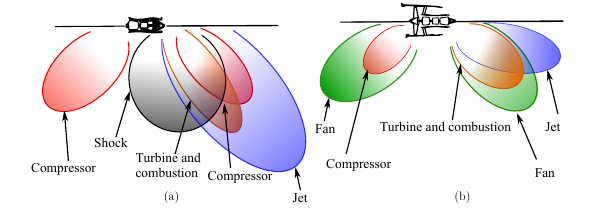
\includegraphics[width=\textwidth]{Chapter-1-Introduction/Figures/lowVhighBPRdirectivitySMITH2004.png}
    \caption{ The evolution of the directivity and the 
    relative levels of sources as a function of engine architecture (a)low bypass-ratio (b) high bypass ratio \cite{smith1989aircraft}}
    \label{fig:intro}
\end{figure}

\section{Statement of the of the research questions}
\subsection{What is already known?}
% III) Research Problem

%   1) What's already known?
%   2) What's missing?
%   3) Why is it a problem?
In general, jet engine designers can model flow within a turbomachine with 
the Navier Stokes (N-S) Equations, a set of partial differential equations that
describe the mass, momentum and energy of a given viscous fluid, however 
these equations can be computationally expensive as they are used in the most
general cases. For aeroacousticians, the N-S equations can be too complicated
to identify sound generation and propagation because acoustic waves are low 
amplitude (~ only a fraction of atmospheric pressure) and are not strongly
influenced by viscosity.   As a result, it is common in practice to 
utilize the Linearized Euler equations (LEE),
a closely related set of PDEs that model inviscid fluid, as they provide an 
approximation for higher Reynold number flows where viscosity 
does not play a critical role. A popular approach to modeling sound propagation 
within a flow is to ``linearize'' the Euler equations, which decomposes the 
flow solution into a mean and fluctuating component . The decomposition is done 
in a linear fashion because the sound propagation amplitude is small with respect
to the mean flow, and their presence does not appreciable change the mean flow 
field. The LEE provides a system of linear equations where for uniform flow, 
the solution is a family of wavenumbers and radial mode shapes that arise from 
unsteady disturbances for flows within a cylindrical duct.  Another method 
decomposes the flow into vortical and potential parts \cite{golubev1996sound}.
In either case, this presents an initial value problem which 
in limited cases can obtain analytical solutions for simplified mean flow. Once a mean flow 
is contains a tangential component, the LEE equations must be solved numerically.  
\subsection{What is missing?/Why is it a problem?}
For uniform flows in a hard wall duct , the waves are categorized as vortical 
,entropical, and acoustic waves. The vortical and entropic waves soley convect with 
the mean flow, where as the acoustic wave can propagate without damping or decay 
exponentially.  However, for swiriling flows, the waves are partially coupled
and are not easily categorized due to an additonal category of ``nearly convecting'' 
modes \cite{Kerrebrock2012},\cite{KERREBROCK1974} . 
Therefore, the families of waves must be found numerically \cite{Envia2004}
making the ducted acoustic propagtion in swirling flow a problem without
an analytical solution but has a framework for a numerical solution.
\subsection{The goal and significance of the investigation}
Swirling flow has been a difficult problem to investigate in comparison to 
flows parallel to the wall domain of a duct \cite{COOPER2001} because of the 
lack of an analytical solution and thus cannot be described from a single convective 
wave equation. However, the solution for sheared mean flows was first presented
by Goldstein \cite{Goldstein1978},\cite{Goldstein1979}. Various special cases of
swirling flow (free vortex and solid body swirl) was examined in \cite{KAPUR1973}
\cite{Kerrebrock2012}, \cite{KERREBROCK1974}. In recent years verification and
validation has been done given the rise in technologies capabale of experimentally
measuring the acoustic modes within a turbomachine \cite{Maldonado2016}. This
work aims offer additional insight to the verification and validation process 
by expanding on techniques used in this field.  
\section{Definition of the terms (if needed)}
\section{Organization of research (Structure)}
% IV) Research aims, objectives, and research question
% V) State benefit/significance
% - speed improvement 
% VI)
% VII)


This research aims to investigave the theoretical framework that is used to
model ducted sound propagation within various flow fields and apply the 
``gold-standard'' of code verification , the method of manufactured solutions 
(MMS) and method of exact solutions (MES) for the limited subset 
of equations where a solution is known, such as uniform mean flow. 


The literature review in the next chapter will discuss the governing equations that are
used to predict the acoustic behavior in a fluid flowing internally, followed 
by the research problem that arises in swirling flow, the objectives and 
questions, the significance and finally the limitations.  The proposed research aims to determine the impact of the numerical schemes used
in the swirling flow problem and how it effects the family of waves that are
produced from the problem formulation so a better understanding of the 
acoustic phenomena as the flow under goes a compressible rotational flow. The use
of the method of manufactured solutions is used as a means of ensuring the code is
correctly approximating the goverining equations and will check the effect of the numerical schemes
on the axial wavenumbers produced.
 
\section{Research Questions and Hypothesis}


- the problem that we're addressing

-- being able to conduct component level code verification tests for the problem
of characterizing the duct acoustics for flow using a LEE model.

why is it a problem? there is multiple ways of arriving at the same solution. 
This can be used to give a metric to either method for the various computational
methods that may be needed to arrive at the final answer.

In the mid 90's,an aeroacoustics model for swirling flow had been proposed and 
has bypassed using a single PDE and has instead used an eigenvalue approach on the 
four governing flow equations. (Why Is this better? does this capturE the problem
differently? why not use the PDE alone instead\ldots)

The proposed component verification from Kleb and Wood will be presented to addreess the characterization of 
modes and the presence of numerical ones. Using higher accuracy methods should 
further improve The result. another thing is to determine how many grid points are needed
for each method



\chapter{Chapter 2: Literature Review}
\section{Introduction}
\subsection{Define your topic and provide an appropriate context for reviewing the literature}
During the 1960's, the increased demand for commercialized aircraft transport 
introduced jet engines capable of supporting large amounts of cargo and passengers. 
On the contrary, this rise in innovation came with a consequence, high volume 
engine noise.  At the time, thee most significant source of noise within an 
aircraft turbo fan engine was attributed to flow interactions between the 
inlet rotor and adjacent stator. 
It is common in turbomachinery to have a stator behind the inlet rotor (or fan) 
to counteract the rotation in the flow due to the rotor. More importantly, 
this configuration causes wakes to form after the rotor, which come into contact 
with the stator. This is denoted as rotor/stator interaction noise \cite{Tyler1962}. 
The ``Tyler-Sofrin selection rule'' (TSSR) was a fundamental contribution 
to the aerospace community, because it is a powerful yet simple 
tool used to quickly determine whether an engine was likely to have 
observable noise emission from the rotor and stator before the engine was manufactured. 
Despite the fact, these preliminary studies were focused on axial compressor noise, the 
TSSR was a pivotal stepping stone. Its application towards modern 
turbomachinery flow has been attempted by modeling the flow as steady in the 
rotating reference frame of the rotor's blade row. However, turbomachinery by 
its very nature produces unsteady flow, and the TSSR in 
not suitable \cite{Holmes2011}. Despite these dissimilarities, the work of 
\cite{Tyler1962} set a strong foundation for the aerospace community, 
allowing for further advances in turbomachinery noise prediction.

\subsection{Establish reasoning - i.e. point - of - view for reviewing the literature}
\subsubsection{Prior work in non-reflecting, non-linear VGBC}
A large amount of aircraft noise was reduced from 1975-2000, 
effectively eliminating the noise pollution for 90\% of the population \cite{Administration}. 
Since the early 2000's, the advancement in noise reduction technologies has been gradual, 
leaving a requirement for drastic improvement in aeroacoustic treatment 
strategies to compete with the demand of quiet subsonic  flight. 
A previous theoretical review by Envia has been suggested that a non linear 
time domain computation could capture the source generation (incident turbulence) 
in addition to the broadband noise. Such a process would have the capabilities 
of  of solving all components of noise generation in an individual calculation \cite{Envia2004}. 
This would at minimum, require an ``LES-type'' fidelity code, which can tend 
to be computationally expensive.  A promising option is NASA GRC's Broadband 
Aeroacoustic Stator Simulation (BASS).  BASS is a high-order, high 
accuracy computational aeroacoustics (CAA) code which has been used to study 
non linear provides mean an extensive study of non linear phenomena in 
turbomachinery flow, and in particular, mechanisms of noise generation that are 
produced from unsteady disturbances. This code allows for a wide variety of 
finite differencing and time marching schemes as well as artificial dissipation methods. This effective computational tool allows for an in-depth modeling of realistic velocity profiles that would be representative of flow produced from a rotor blade row. In recent work, a new method of implementing realistic, three-dimensional rotor wakes free from acoustics was validated  \cite{Hixon2011}. This provides a means of studying acoustic responses non linear swirling flows within pragmatic geometric configurations, while simultaneously allow for the modeling of sources generation produced from the incident turbulence. 

\subsection{Explain the order/sequence of the review}
This review will compare studies that have considered the applicability of unsteady linearized Euler equations on cylindrical and annular ducts. First the work of Kousen will breifly summarized \cite{Kousen1996,Kousen1999}. Secondly, the alternate approached shown by Golubev and Atassi used in \cite{Golubev1996,Golubev1998} were also compared. These works have utilized a standard normal mode approach to determine the modal response of inviscid, compressible, swirling flow within a cylindrical and annular ducts. Results and findings have revealed three categories of associated wave - modes, acoustic, nearly convected, and nearly sonic. Detailed examination of the literature indicate that the hierarchical system was not initially apparent. A qualitative description of the numerical methods used to evaluate the eigensystem of solutions will be described.

One key question that remains, is how well do unsteady linearized equations capture the mechanisms of noise generation within realistic turbomachinery flow? There exists a copious amount of published work describing the use of wave equations to describe the governing behavior of ducted sound propagation(See \cite{Michel2008} for extensive preliminary review). However, turbomachines inherently rely on high velocities, high temperatures to maximize efficiencies. Such mechanisms need a more thorough formulation so that a complete acoustic description of the flow can be provided. Large contributions were first made by Kousen and Atassi and as a result they will be used for comparison.

%To begin exploring various geometries, we must first ask: what are the central theories that have been used `````````````````````````````````````````````````````````````````````````````````````````````````````````````````````````````112\sqrt{`312` explain the acoustic behavior of unsteady swirling flows? Do the linearized Euler equations provide an adequate means of capturing the mechanisms of noise generation within realistic turbomachinery flow? This paper will explore prior theories used to explain this and their methodologies. Large contributions were first made by Koussen and Atassi and as a result they will be used for comparison. Tam proposed a theoretical framework where the modes of a flow are characterized by an initial boundary value problem, allowing for the appearance of ''continuum modes`` \cite{Tarn1998}
\subsection{State the scope (what is included and what is not)}
This review will be a qualitative report of the findings, but a quantitative comparison ''meta-analysis`` should be done for potentially ideal test cases.

The study was expanded by \cite{KERREBROCK1974,YURKOVICH1975} who
included cases of solid body swirl. Wundrow studied the swirling potential flows using Goldstein's disturbance velocity
decomposition \cite{Goldstein1978} using a numerical approach and found that the solutions
were more accurate and found more efficiently \cite{KERREBROCK1974}. Kousen expanded these efforts by including \cite{kousen1996pressure,kousen1995eigenmode} the effect unsteady disturbances in the presence of 
forced solid body-swirl and free-vortex flow without the use of potential flow theory. Using normal 
mode analysis along with a radial spatial differencing scheme, the wave modes produced within cylindrical and annular ducts was 
reported. Results show (figure 4.7) two distinct families of modes, purely convected and acoustic 
modes. The presence of axial shear in combination solid body flows can endue coupling between these modes, which 
in theory would not appear unless viscous terms were present in the eigenvalue analysis. Lack of available swirl flow 
results ``hampered'' validation attempts. However, this eigenvalue approach was utilized with a new quasi-3D 
formulation to find the axial wavenumbers from solid body flow was proposed in his next work . 

In \cite{kousen1995eigenmode}, A quasi 3D formulation was validated and used to predict 
the appearance of modes due to the interaction of a rotor with spatially 
uniform steady and unsteady flow. These modes were first classified by 
\cite{Tyler1962} as ``spinning modes''. In addition, further investigation was 
done on the results shown in \cite{kousen1995eigenmode}. The axial wavenumbers that 
were previously found to be purely convective were shown to be in part
,``nearly convective'' (shear) pressure modes. These were found to propagate in the 
axial direction with no loss in amplitude, thus never satisfying the cut-off condition. 



\section{Golubev and Atassi's work}
Similarly, a narrow annulus is once again 
studied but with a different theoretical and computational approach. The governing equations, similar to Wundrow \cite{Wundrow2019} were still then linearized in terms of potential and rotation. As suggested by Case \cite{Case2004}, a Fourier series analysis was used to conduct the normal mode analysis to find the corresponding wave numbers 
of the eigensystem. The findings show these fall into further classification which were previously denoted as purely convective and 
in part, nearly-convective wave modes. These two classifications of purely convective disturbance can be split into 
their ``nearly-convected vorticity dominated'' and ``nearly-sonic pressure dominated'' parts. These new 
results show the appearance of ``nearly-sonic pressure dominated modes'' which can propagate at varying phase speeds 
throughout the duct in both directions. The imposed Doppler shift from asymmetrical modes cause the sound propagate in the 
opposite direction of the mean flow swirl. A weak coupling relation relates the two and allows for the presence 
of vorticity - pressure mode coupling. Together, these nearly convected modes can be ``identified with the purely 
convective gusts in a non swilirling flow''. For the second group, these ``nearly convected'' vorticity dominated 
modes are further split as these disturbances approach the \textit{critical layer}, i.e. the 
location at which the viscous effects of the boundary layer begin to influence the coupling between modes. When both 
solid body and free vortex induced rotations are in the same direction, no instabilities arise from outside the critical 
layer. It was shown in later works that the influence of centrifugal and Coriolis forces created by the mean 
swirl prevent the decomposition of modes into their potential, rotational and entropic components. The paper ultimately proposes ``
a generalized definition for incident rotational waves(gusts) is proposed which accounts for both the eigenmodes and the 
initial value solutions'' 
%\section{Idea one. Central acoustic theory for unsteady ducted flow}
%\subsubsection{Main Idea - Uniform Mean Flow}
%In ducted turbomachinery, the appearance of unsteady flow has been first understood by characterizing the acoustic response of small disturbances. These small disturbances amount to modal content that govern the behavior of these responses. 
%\subsubsection{Evidence}
%It was shown by (Verdon:1989) that any small disturbance can be represented at a decomposition of acoustic, vortical, and entropic components. However, in the presence of sheared mean axial floww, the acoustic response of the mean flows that arise cannot be described in the same manner and cannot be solved analytically, calling for numerical approaches \cite{Kousen1996}. Preliminary results show that these responses fall into convective and ``non-convective'' classifications.
%\subsubsection{Analysis}
%Complex analysis allows us to observe the phase change in these mode shapes which can comprise the entire continua of the flow domain
%\subsubsection{Lead Out}

%\subsection{Concept}
%\subsubsection{Main Idea}
%The classification of modes into ``convected'', ``non-convected'' and ``nearly convected''
%\subsubsection{Evidence}
%\subsubsection{Analysis}
%\subsubsection{Lead Out}


%Tyler Sofrin selection rule serves well for rotor and stators that are evenly spaced. 
%- Utilizes the fourier transform


\section{Conclusion}
\begin{itemize}
    \item The conclusion summarizes 
        the key findings of the review in general terms. Notable commonalities between works, whether favorable or not
        , may be included here.
        \subitem This review discusses the development of the unsteady linearized equations, 
        and how improvements in the modal analysis capture more families of mechanisms of noise generation within non-uniform 
        swirling flow turbomachinery flow. 
    \item This section is the reviewer’s opportunity to justify a research 
        proposal. Therefore, the idea should be clearly re-stated and supported according to the findings of 
        the review.
        \subitem This literature review should be expanded to describe specific details in the methodologies and validation techniques reported by \cite{Kousen1996,Kousen1999,Golubev1996,Golubev1998}. 
\end{itemize}


\chapter{Chapter 3: Methods}
\section{Aerodynamic Models}
\subsection{Steady Models}
\subsection{Setting up SWIRL's Aerodynamic Model}
The Euler Equations in Cylindrical Form are,
\begin{align*}
\frac{\partial \rho}{\partial t} + %Conservation of mass
v_r \frac{\partial \rho}{\partial r} +
\frac{v_{\theta}   }{r}
\frac{\partial \rho}{\partial \theta} +
v_x \frac{\partial \rho}{\partial \theta} + 
\rho 
\left(
\frac{1}{r} \frac{\partial (rv_r)	}{\partial r} +
\frac{1}{r}	\frac{\partial v_{\theta}}{\partial \theta} +
\frac{\partial v_x}{\partial x}
\right) 
&= 0 \\% \label{ConservationOfMass} %%%%%%%%%%%%%%%%%%%%%%%%%%%%%%%%%%%%%%
\frac{\partial v_r}{\partial t} + 
v_r \frac{\partial v_r}{\partial r} +
\frac{v_{\theta}  }{r}
\frac{\partial v_r}{\partial \theta}- \frac{v_{\theta}^2}{r}+ 
v_x \frac{\partial v_r}{\partial x} 
&= -\frac{1}{\rho} \frac{\partial p}{\partial r}\\  
\frac{\partial v_{\theta}}{\partial t} + 
v_r \frac{\partial v_{\theta}}{\partial r} +
\frac{v_{\theta}}{r}
\frac{\partial v_{\theta}}{\partial \theta} +
\frac{v_r v_{\theta}}{r}+ 
v_x \frac{\partial v_{\theta}}{\partial x} 
&= -\frac{1}{\rho r} \frac{\partial p}{\partial \theta}\\ 
\frac{\partial v_{x}}{\partial t} + 
v_r 
\frac{\partial v_x}{\partial r} +
\frac{v_{\theta}}{r}
\frac{\partial v_x}{\partial \theta}+ 
v_x \frac{\partial v_x}{\partial x} 
&= 
-\frac{1}{\rho } 
\frac{\partial p}{\partial x}\\  
\frac{\partial p }{\partial t} +
v_r 
\frac{\partial p}{\partial r} +
\frac{v_{\theta}}{r}
\frac{\partial p}{\partial \theta} +
v_x \frac{\partial p}{\partial \theta} + 
\gamma p 
\left(
\frac{1}{r}\frac{\partial (rv_r)}{\partial r} +
\frac{1}{r}\frac{v_{\theta}}{\partial \theta} +
\frac{\partial v_x}{\partial x}
\right) &= 0
\end{align*}


\section{Mean Flow Equations}

SWIRL utilizes the following assumptions,

\begin{itemize}
    \item No flow in the radial direction. Consequentially, the flow is 
        axisymmetric along the downstream direction.
    \item No surface or body forces
    \item Isentropic conditions 
\end{itemize}

For steady flow, the continuity, momentum and entropy equations are

\[\nabla (\vec{V} \bar{\rho}) = 0\]
\[(\vec{V}\cdot \nabla) \vec{V}\]
\[\nabla S = 0\]

If we neglect radial velocity, the velocity vector in cylindrical coordinates are

\[\vec{V}(r,\theta,x) = V_x(r) \hat{e}_x + V_{\theta} (r) \hat{e}_{\theta} \]
Starting with the radial momentum equation, 
\begin{align*}
\frac{\partial v_r}{\partial t} + 
v_r \frac{\partial v_r}{\partial r} +
\frac{v_{\theta}  }{r}
\frac{\partial v_r}{\partial \theta}- \frac{v_{\theta}^2}{r}+ 
v_x \frac{\partial v_r}{\partial x} 
&= -\frac{1}{\rho} \frac{\partial p}{\partial r} 
\end{align*}
See Appendix for speed of sound derivation

\section{Applying model to various flows}
The LEE for flows ith axial sheared flow, solid body and free vortex swirl
were reviewed by \cite{kousen1995eigenmode}, and most recently studied by \cite{Maldonado2016}.
\subsection{Axial Shear Flow}
In \cite{kousen1995eigenmode}, axial sheared flows through a constant area duct was 
investigated.The only effect on the velocity gradient occurs along the x axis. 
All other primitive variables (pressure and density which is $\propto$ speed of
sound) are constant. As a result, the only changes that occur are in the x
direction. This implies that $\partial / \partial \theta = 0$. 
For the conservation of mass,

\[ \nabla (\vec{V}\bar{\rho}) =  \left( 
\underbrace{
	\cancel{
		\frac{\partial (\bar{\rho}v_r)	}{\partial r}
	}
}_{v_r = 0} +
\underbrace{\cancel{\frac{1}{r}	\frac{\partial \bar{\rho}v_{\theta}}{\partial \theta}}}_{\frac{\partial }{\partial \theta}} +
\frac{\partial \bar{\rho}v_x}{\partial x}
\right) = \frac{\partial \bar{\rho}v_x}{\partial x}\] 

The conservation of momentum in the radial direction becomes:
\[(\vec{V}\cdot \nabla) \vec{V} =
\cancel{v_r \frac{\partial v_r}{\partial r}} +
\cancel{\frac{v_{\theta}  }{r}
	\frac{\partial v_r}{\partial \theta}}- \frac{v_{\theta}^2}{r}+ 
\cancel{v_x \frac{\partial v_r}{\partial x} }
= -\frac{1}{\rho} \frac{\partial P}{\partial r}
\]
\[
\frac{v_{\theta}^2}{r}
= \frac{1}{\rho} \frac{\partial P}{\partial r}
\] 

\[
\frac{{\rho} v_{\theta}^2}{r} 
=\frac{\partial P}{\partial r}
\]
For the $\theta$ direction,
\[(\vec{V}\cdot \nabla) \vec{V} = \cancel{v_r \frac{\partial v_{\theta}}{\partial r} +
	\frac{v_{\theta}}{r}
	\frac{\partial v_{\theta}}{\partial \theta} +
	\frac{v_r v_{\theta}}{r}}+ 
v_x \frac{\partial v_{\theta}}{\partial x} 
= \cancel{-\frac{1}{\rho r} \frac{\partial P}{\partial \theta}}\]
Dividing $v_x$ to the other side,
\[ \frac{\partial v_{\theta}}{\partial x}  = 0\]

Similarly for the $x$ direction,

\[ \frac{\partial v_x}{\partial x} = 0 \]
In regards to the entropy equation, having an isentropic flow, $\nabla S = 0$ implies $A^2= \frac{\nabla \bar{P}}{ \nabla \bar{\rho}}$ 


\section{Accounting for solid body swirl}

If the flow contains a swirling component, then the primitive variables are 
nonuniform through the flow, and mean flow assumptions are not valid. 
To account to this, we integrate the momentum equation in the radial direction 
with respect to the radius. 

Equation (2.5) in \cite{kousen1995eigenmode} is 

\[P = \int_{\tilde{r}}^{1} \frac{\bar{\rho} V_{\theta}^2}{\tilde{r}} d\tilde{r}\] 

where $\tilde{r}$ is the radius dimensional radius normalized by the tip diameter $r_t = r_{max}$

The dimensional form is,
\[
\frac{\bar{\rho} v_{\theta}^2}{r} 
=\frac{\partial P}{\partial r}
\]
By appplying separation of variables, the expression for $P$ can be found,
\[
\int_{r}^{r_{max}} \frac{\bar{\rho} v_{\theta}^2}{r}\partial r 
=-\int_{P(r)}^{P(r_{max})}\partial P
\]

Since $\tilde{r} = r/r_{max}$ then,
\[r = \tilde{r}r_{max}\]
by taking total derivatives and applying chain rule,

\[dr = d(\tilde{r}r_{max}) = d(\tilde{r})r_{max}\]
Substituting these terms back in and evaluating the right hand side,
\[
\int_{\tilde{r}}^{1} \frac{\bar{\rho} v_{\theta}^2}{\tilde{r}}\partial \tilde{r} 
=P(1)-P(\tilde{r})
\]
For reference the minimum value of $\tilde{r}$ is

\[\sigma = \frac{r_{max}}{r_{min}}\]

The radial derivative of the speed of sound squared is then used to find the 
speed of sound in the cases where there is mean tangetial component regardless
of there being axial flow,

\[\frac{\partial A^2}{\partial r } = \frac{\partial}{\partial r} \left( \frac{\gamma P}{\rho} \right)\]
Using the quotient rule, the definition of the speed of sound is found to be ,
\begin{align*}
&= \frac{\partial P}{\partial r} \frac{\gamma \bar{\rho}}{\bar{\rho}^2} - \left( \frac{\gamma P}{\bar{\rho}^2} \right) \frac{\partial \bar{\rho}}{\partial r}\\
&=  \frac{\partial P}{\partial r} \frac{\gamma }{\bar{\rho}} - \left( \frac{A^2}{\bar{\rho}} \right) \frac{\partial \bar{\rho} }{\partial r}\\ \text{Using } \partial P/A^2 = \partial \rho \rightarrow &= \frac{\partial P}{\partial r} \frac{\gamma }{\bar{\rho}} - \left( \frac{1}{\bar{\rho}} \right) \frac{\partial \bar{ P} }{\partial r}\\
\frac{\partial A^2}{\partial r} &= \frac{\partial P}{\partial r} \frac{\gamma - 1}{\bar{\rho}}  \\ \text{or..}
\frac{\bar{\rho}}{\gamma -1}\frac{\partial A^2}{\partial r} &= \frac{\partial P}{\partial r} 
\end{align*}


Going back to the radial momentum equation , and rearranging the 
\begin{align*}
\frac{\bar{\rho} v_{\theta}^2}{r} 
&=\frac{\partial P}{\partial r}\\
\frac{\cancel{\bar{\rho}} v_{\theta}^2}{r} 
&=\frac{\cancel{\bar{\rho}}}{\gamma -1}\frac{\partial A^2}{\partial r}\\
\frac{v_{\theta}^2}{r}\left(\gamma -1\right) &= \frac{\partial A^2}{\partial r}\\ \text{Dividing both sides by } A^2 \rightarrow \frac{M_{\theta}}{r}\left(\gamma - 1\right) &= \frac{\partial A^2}{\partial r} \frac{1}{A^2}
\end{align*}
\begin{align*}
\text{Integrating both sides } \int_{r}^{r_{max}}\frac{M_{\theta}}{r}\left(\gamma - 1\right){\partial r}  &=\int_{A^2(r)}^{A^2(r_{max})}\frac{1}{A^2}  {\partial A^2}\\
\int_{r}^{r_{max}}\frac{M^2_{\theta}}{r}\left(\gamma - 1\right){\partial r}  &=ln(A^2(r_{max})) - ln(A^2(r)) \\
\int_{r}^{r_{max}}\frac{M^2_{\theta}}{r}\left(\gamma - 1\right){\partial r}  &=ln\left(\frac{A^2(r_{max})}{A^2(r)}\right) 
\end{align*}

Defining non dimensional speed of sound $\tilde{A} = \frac{A(r)}{A(r_{max})}$
\begin{align*}
\int_{r}^{r_{max}}\frac{M_{\theta}}{r}\left(\gamma - 1\right){\partial r}  &=ln\left(\frac{1}{\tilde{A}^2}\right) \\
&= -2ln(\tilde{A})\\
\tilde{A}(r) &= exp\left[-\int_{r}^{r_{max}}\frac{M_{\theta}}{r}\frac{\left(\gamma - 1\right)}{2}{\partial r}\right] \\ \text{replacing r with }\tilde{r} \rightarrow \tilde{A}(r) &= exp\left[-\int_{r}^{r_{max}}\frac{M_{\theta}}{r}\frac{\left(\gamma - 1\right)}{2}{\partial r}\right]		\\
\tilde{A}(\tilde{r}) &= exp\left[\left(\frac{1 - \gamma}{2}\right)\int_{\tilde{r}}^{1}\frac{M_{\theta}}{\tilde{r}}{\partial \tilde{r}}\right]	
\end{align*}

\subsection{Unsteady Models}
% 
\subsection{Linearizing the governing equations}
\subsubsection{Linearizing Conservation of Mass}
To linearize the Euler equations, we substitute each flow variable with its equivalent mean and perturbation components. Note that the mean term is only a function of space whereas the perturbation component is a dependent on both space and time (functional dependence is not explicity written with each variable). Assuming that we can divide the variable into a known laminar flow solution to the Navier-Stokes equations and a small amplitude perturbation solution:

%\begin{align}
%v_r 		&= V_r(x) + v_r'\\
%v_{\theta} 	&= V_{\theta} + v_{\theta}'\\
%v_x 		&= V_x + v_x'\\
%p 			&= \bar{p} + p'\\
%\rho 		&= \bar{\rho} + \rho'
%\end{align}
%% \newpage
%% Starting with continuity,
%Substituting these expressions into the governing equations will give the 
%linearized perturbation equations for swirling flows in cylindrical coordinates,
%%\begin{flushleft}
%\begin{equation*} 
%\end{equation*}
%\begin{align*}
%\frac{\partial \rho}{\partial t} + 
%v_r \frac{\partial \rho}{\partial r} +
%\frac{v_{\theta}   }{r}
%\frac{\partial \rho}{\partial \theta} +
%v_x \frac{\partial \rho}{\partial \theta} + 
%\rho 
%\left(
%\frac{1}{r} \frac{\partial (rv_r)	}{\partial r} +
%\frac{1}{r}	\frac{\partial v_{\theta}}{\partial \theta} +
%\frac{\partial v_x}{\partial x}
%\right) 
%= 0\\
%\frac{\partial \bar{\rho} + \rho' }{\partial t} +
%(V_r + v_r') 
%\frac{\partial \bar{\rho} + \rho'}{\partial r} +
%\frac{V_{\theta} + v_{\theta}'}{r}
%\frac{\partial \bar{\rho} + \rho'}{\partial \theta} +
%(V_x + v_x') 
%\frac{\partial \bar{\rho} + \rho'}{\partial \theta} + \\ 
%(\bar{\rho} + \rho') 
%\left(
%\frac{1}{r}\frac{\partial (r(V_r +v_r'))}{\partial r} +
%\frac{1}{r}\frac{\partial V_{\theta}+v_{\theta}'}{\partial \theta} +
%\frac{\partial (V_x + v_x')}{\partial x}
%\right) = 0\\
%\frac{\partial \bar{\rho}}{\partial t} + 
%\frac{\partial \rho'     }{\partial t} +\\
%V_r \frac{\partial \bar{\rho}}{\partial r} +  
%v_r'\frac{\partial \bar{\rho}}{\partial r} + 
%V_r \frac{\partial \rho'}{\partial r} +
%v_r'\frac{\partial \rho'}{\partial r} + \\
%\frac{1}{r}
%\left(
%V_{\theta} \frac{\partial \bar{\rho}}{\partial \theta} +
%v_{\theta}'\frac{\partial \bar{\rho}}{\partial \theta} + 
%V_{\theta} \frac{\partial \rho'		}{\partial \theta} + 
%v_{\theta}'\frac{\partial \rho'		}{\partial \theta}
%\right) + \\ 
%V_x \frac{\partial \bar{\rho}}{\partial x} + 
%v_x'\frac{\partial \bar{\rho}}{\partial x} +
%V_x \frac{\partial \rho'	 }{\partial x} 	+
%v_x'\frac{\partial \rho'    }{\partial x}		+\\
%\bar{\rho} 
%\left(
%\frac{1}{r}
%\left(
%\frac{\partial (rV_r  )    }{\partial r} +
%\frac{\partial (r(v_r')    }{\partial r} +
%\frac{\partial V_{\theta}  }{\partial \theta} +
%\frac{\partial v_{\theta}' }{\partial \theta}
%\right) +
%\frac{\partial V_x }{\partial x} +
%\frac{\partial v_x'}{\partial x}
%\right) + \\
%\rho'
%\left(
%\frac{1}{r}
%\left(
%\frac{\partial (rV_r  )    }{\partial r} +
%\frac{\partial (r(v_r')    }{\partial r} +
%\frac{\partial V_{\theta}  }{\partial \theta} +
%\frac{\partial v_{\theta}' }{\partial \theta}
%\right) +
%\frac{\partial V_x }{\partial x} +
%\frac{\partial v_x'}{\partial x}
%\right)
%= 0	\\
%\end{align*}
%\end{flushleft}
Important things to note
\begin{itemize}
	\item The small disturbances are infinitesimal (thus linearized)
	\item Neglect second order terms.
	\item The continuity equation is comprised of mean velocity components. This is subtracted off in each of the governing equations
\end{itemize}

% Blue will be used for terms that are removed after subtracting in the original continuity equation, green will be used to cancel higher(2nd) order terms.Red will be used if we take the radial velocity to be zero.

% \begin{align*}
% =
% \Ccancel[blue]
% {\frac{\partial \bar{\rho}}{\partial t}} + 
% \frac{\partial \rho'     }{\partial t} + \\
% \Ccancel[blue]  {V_r \frac{\partial \bar{\rho}}{\partial r}} +  
% \Ccancel[blue] {v_r'\frac{\partial \bar{\rho}}{\partial r}} + 
% \Ccancel[red]{V_r \frac{\partial \rho'}{\partial r}} +
% \Ccancel[green]{v_r'\frac{\partial \rho'}{\partial r}} + \\
% \frac{1}{r}
% \left(
% \Ccancel[blue]{V_{\theta} \frac{\partial \bar{\rho}}{\partial \theta}} +
% \Ccancel[blue]{v_{\theta}'\frac{\partial \bar{\rho}}{\partial \theta}} + 
% V_{\theta} \frac{\partial \rho'		}{\partial \theta} + 
% \Ccancel[green]{v_{\theta}'\frac{\partial \rho'		}{\partial \theta}}
% \right) + \\ 
% \Ccancel[blue]{V_x \frac{\partial \bar{\rho}}{\partial x}} + 
% \Ccancel[blue]{v_x'\frac{\partial \bar{\rho}}{\partial x}} +
% V_x \frac{\partial \rho'	 }{\partial \theta} 	+
% \Ccancel[green]{v_x'\frac{\partial \rho'    }{\partial x}}		+\\
% \bar{\rho} 
% \left(
% \frac{1}{r}
% \left(
% \Ccancel[blue]{\frac{\partial (rV_r  )    }{\partial r}} +
% \frac{\partial (r(v_r')    }{\partial r} +
% \Ccancel[blue]{\frac{\partial V_{\theta}  }{\partial \theta}} +
% \frac{\partial v_{\theta}' }{\partial \theta}
% \right) +
% \Ccancel[green]{\frac{\partial V_x }{\partial x}} +
% \frac{\partial v_x'}{\partial x}
% \right) + \\
% \rho'
% \left(
% \frac{1}{r}
% \left(
% \Ccancel[blue]{\frac{\partial (rV_r  )    }{\partial r}} +
% \Ccancel[green]{\frac{\partial (r(v_r')    }{\partial r} }+
% \Ccancel[blue]{\frac{\partial V_{\theta}  }{\partial \theta} }+
% \Ccancel[green]{\frac{\partial v_{\theta}' }{\partial \theta}}
% \right) +
% \Ccancel[blue]{\frac{\partial V_x }{\partial x}} +
% \Ccancel[green]{\frac{\partial v_x'}{\partial x}} = 0
% \right)
% \end{align*}

% \begin{align*}
% \boxed{
% 	\frac{\partial \rho'}{\partial t} +
% 	\frac{V_{\theta}}{r}
% 	\frac{\partial \rho'}{\partial \theta} + 
% 	V_x
% 	\frac{\partial \rho'}{\partial x} +
% 	\bar{\rho}
% 	\left(
% 	\frac{1}{r}
% 	\left(
% 	\frac{\partial r v_r'}{\partial r} + \frac{\partial v_{\theta}'}{\partial \theta}		 
% 	\right) +
% 	\frac{\partial v_x'}{\partial x}
% 	\right)= 0} 
% \end{align*}
% \newpage
% \subsubsection{Linearizing the Conservation of Momentum\\ in the \textit{r} direction}
% Starting with the mean momentum equation 
% \begin{align*}
% \frac{\partial v_r}{\partial t} + 
% v_r \frac{\partial v_r}{\partial r} +
% \frac{v_{\theta}  }{r}
% \frac{\partial v_r}{\partial \theta}- \frac{v_{\theta}^2}{r}+ 
% v_x \frac{\partial v_r}{\partial x} 
% &= -\frac{1}{\rho} 
% \frac{\partial p}{\partial r}
% \end{align*}
% Looking at the left hand side first
% \begin{align*} 
% \frac{\partial (V_r + v_r') }{\partial t} + 
% ( V_r + v_r' ) 
% \frac{\partial( V_r + v_r')}{\partial r} +
% \frac{V_{\theta} + v_{\theta}'}{r}
% \frac{\partial(V_r + v_r')}{\partial \theta} -
% \frac{ (V_{\theta} + v_{\theta}')^2}{ r} + 
% (V_x + v_x') 
% \frac{\partial (V_r + v_r')}{\partial x} 	
% &= -\frac{1}{\rho} \frac{\partial p}{\partial r}\\
% \Ccancel[blue]  {\frac{\partial  V_r  }{\partial t}}	+
% \frac{\partial  v_r' }{\partial t} + \\
% \Ccancel[blue]  {V_r  \frac{\partial  V_r  }{\partial r}}  +
% \Ccancel[blue] {v_r' \frac{\partial  V_r  }{\partial r}} + 
% \Ccancel[red] {V_r  \frac{\partial  v_r' }{\partial r}} + 
% \Ccancel[green]{v_r' \frac{\partial  v_r' }{\partial r}} +\\
% \frac{1}{r}
% \left(
% \Ccancel[blue]  {V_{\theta} \frac{\partial V_r}{\partial \theta}} +
% \Ccancel[blue] {v_{\theta}'\frac{\partial V_r}{\partial \theta}} +
% V_{\theta} \frac{\partial v'_r}{\partial \theta} +
% \Ccancel[green]{v_{\theta}'\frac{\partial v'_r}{\partial \theta}}
% \right)- \\
% \frac{1}{r}\left(
% \Ccancel[blue]{V_{\theta}^2} + 
% 2V_{\theta}v'_{\theta} + 	
% \Ccancel[green]{v^{'2}_{\theta}}\right)+\\
% \Ccancel[blue]{V_x \frac{\partial V_r }{\partial x}} +
% \Ccancel[blue]{v_x'\frac{\partial V_r }{\partial x}} +  
% V_x \frac{\partial v_r'}{\partial x} +
% \Ccancel[green]{v_x' \frac{\partial v_r'}{\partial x}} 
% &= -\frac{1}{\rho} 
% \frac{\partial p}{\partial r}\\
% \frac{\partial  v_r' }{\partial t} +
% V_r  \frac{\partial  v_r' }{\partial r} + 
% \frac{V_{\theta}}{r} \frac{\partial v'_r}{\partial \theta} -
% \frac{2V_{\theta}v'_{\theta}}{r} +
% V_x \frac{\partial v_r'}{\partial x} 
% &= -\frac{1}{\rho} 
% \frac{\partial p}{\partial r}
% \end{align*}
% \newpage
% Now looking at the right side,
% Expanding the $1/\rho $ using a Taylor series approximation

% \begin{align*}
% \frac{1}{\bar{\rho} + \rho'} 
% &= \frac{1}{\bar{\rho}} 
% + \left(
% \frac{1}{\bar{\rho} 
% 	+ \rho'} 
% - \frac{1}{\rho}
% \right) \\
% &= \frac{1}{\bar{\rho}} 
% + \left(
% \frac{\bar{\rho}}{\bar{\rho}(\bar{\rho} 
% 	+ \rho')} 
% - \frac{1}{\rho} \frac{\bar{\rho} + \rho'}{\bar{\rho} + \rho'}
% \right) \\
% &= \frac{1}{\bar{\rho}} 
% - \left(
% \frac{\bar{\rho} - \bar{\rho} + \rho'}{\bar{\rho}(\bar{\rho} 
% 	+ \rho')}
% \right)	\\
% &= \frac{1}{\bar{\rho}} 
% - \frac{\rho'}{\bar{\rho}}
% \underbrace{\left(
% 	\frac{1}{\bar{\rho} + \rho}
% 	\right)}_\text{This is what we're solving for!}	\\
% &= \frac{1}{\bar{\rho}} 
% - \frac{\rho'}{\bar{\rho}}
% \underbrace{
% 	\left[\frac{1}{\bar{\rho}} 
% 	+ \left(
% 	\frac{1}{\bar{\rho} 
% 		+ \rho'} 
% 	- \frac{1}{\rho}
% 	\right) \right] }_\text{This is from step 1}	\\
% &= \frac{1}{\bar{\rho}} 
% - \frac{\rho'}{\bar{\rho}^2} +
% \underbrace{
% 	\left[ \left(\frac{\rho'}{\bar{\rho}}\right)^2
% 	\frac{1}{\bar{\rho} 
% 		+ \rho'} 
% 	\right] }_\text{These are higher order terms that will go to $\infty$}	\\	
% \end{align*}
% \begin{align*} % \text{Plugging this back in to the right hand side, (don't forget the negative!)} \rightarrow
% \frac{1}{\rho}\frac{\partial p}{\partial r} = \left( -\frac{1    }{\bar{\rho}} +
% \frac{\rho'}{\bar{\rho}^2}\right) \left(\frac{\partial \bar{p} + p'}{\partial r}\right)\\
% \frac{1}{\rho}\frac{\partial p}{\partial r} =  -\Ccancel[blue]{\frac{1    }{\bar{\rho}}  \frac{\partial \bar{p}}{\partial r}} -  
% \frac{1    }{\bar{\rho}}  \frac{\partial p'}{\partial r} +
% \frac{\rho'}{\bar{\rho}^2}\frac{\partial \bar{p}}{\partial r} +
% \Ccancel[green]{\frac{\rho'}{\bar{\rho}^2}\frac{\partial p'}{\partial r}}\\
% \frac{1}{\rho}\frac{\partial p}{\partial r} =  -\frac{1    }{\bar{\rho}}  \frac{\partial p'}{\partial r} +
% \frac{\rho'}{\bar{\rho}^2}\frac{\partial \bar{p}}{\partial r} 
% \end{align*}

% \begin{align*}
% \boxed{
% 	\frac{\partial  v_r' }{\partial t} +
% 	\frac{V_{\theta}}{r} \frac{\partial v'_r}{\partial \theta} -
% 	\frac{2V_{\theta}v'_{\theta}}{r} +
% 	V_x \frac{\partial v_r'}{\partial x} =\frac{1    }{\bar{\rho}}  \frac{\partial p'}{\partial r} +
% 	\frac{\rho'}{\bar{\rho}^2}\frac{\partial \bar{p}}{\partial r} 
% }
% \end{align*}
% \newpage
% \subsubsection{Linearizing the Conservation of Momentum\\ in the \textit{$\theta$} direction}
% Starting with the mean momentum equation 
% \begin{align*}
% \frac{\partial v_{\theta}}{\partial t} + 
% v_r \frac{\partial v_{\theta}}{\partial r} +
% \frac{v_{\theta}  }{r}
% \frac{\partial v_{\theta}}{\partial \theta}+
% \frac{v_r v_{\theta}}{r}+ 
% v_x \frac{\partial v_{\theta}}{\partial x} 
% &= -\frac{1}{\rho r} 
% \frac{\partial p}{\partial \theta}
% \end{align*}

% Looking at the left hand side first
% \begin{align*} 
% \frac{\partial (V_{\theta} + v_{\theta}') }{\partial t} + 
% ( V_r + v_r' ) 
% \frac{\partial( V_{\theta} + v_{\theta}')}{\partial r} + \\
% \frac{V_{\theta} + v_{\theta}'}{r}
% \frac{\partial(V_{\theta} + v_{\theta}')}{\partial \theta} +
% \frac{ (V_r + v_r')(V_{\theta} + v_{\theta}')}{ r} + 
% (V_x + v_x') 
% \frac{\partial (V_{\theta} + v_{\theta}')}{\partial x} 	
% &= 
% -\frac{1}{\rho r} \frac{\partial p}{\partial \theta}\\
% \Ccancel[blue]  {\frac{\partial  V_{\theta}  }{\partial t}}	+
% \frac{\partial  v_{\theta}' }{\partial t} + \\
% \Ccancel[blue]  {V_r  \frac{\partial  V_{\theta}  }{\partial r}}  +
% \underbrace{v_r' \frac{\partial  V_{\theta}  }{\partial r}}_{v_r'=0} + 
% \Ccancel[red]{V_r  \frac{\partial  v_{\theta}' }{\partial r}} + 
% \Ccancel[green]{v_r' \frac{\partial  v_{\theta}' }{\partial r}} +\\
% \frac{1}{r}
% \left(
% \Ccancel[blue]  {V_{\theta} \frac{\partial V_{\theta}}{\partial \theta}} +
% \Ccancel[blue] {v_{\theta}'\frac{\partial V_{\theta}}{\partial \theta}} +
% V_{\theta} \frac{\partial v'_{\theta}}{\partial \theta} +
% \Ccancel[green]{v_{\theta}'\frac{\partial v'_{\theta}}{\partial \theta}}
% \right)+ \\
% \frac{1}{r}\left(
% \Ccancel[blue]{V_r V_{\theta}} + 
% v_r'V_{\theta} +
% \Ccancel[red]{V_r v'_{\theta}}  + 	
% \Ccancel[green]{v_r'v_{\theta}'}\right)+\\
% \Ccancel[blue]{V_x \frac{\partial V_{\theta} }{\partial x}} +
% \Ccancel[blue]{v_x'\frac{\partial V_{\theta} }{\partial x}} +  
% V_x \frac{\partial v_{\theta}'}{\partial x} +
% \Ccancel[green]{v_x' \frac{\partial v_{\theta}'}{\partial x}} 
% &= -\frac{1}{\rho r} 
% \frac{\partial p}{\partial \theta}\\
% \frac{\partial  v_{\theta}' }{\partial t} +
% v_r' \frac{\partial  V_{\theta}  }{\partial r} +
% \frac{V_{\theta}}{r} \frac{\partial v'_{\theta}}{\partial \theta} +
% \frac{v'_rV_{\theta}}{r} +
% V_x \frac{\partial v_r'}{\partial x} 
% &= -\frac{1}{\rho r} 
% \frac{\partial p}{\partial \theta}
% \end{align*}
% Now looking at the right side,
% Expanding the $1/\rho $ using a Taylor series approximation

% \begin{align*}
% &
% -\frac{1}{\rho r}\frac{\partial p}{\partial \theta} = \left( -\frac{1    }{\bar{\rho}} +
% \frac{\rho'}{\bar{\rho}^2}\right) \left(\frac{\partial \bar{p} + p'}{\partial \theta}\right)\\
% &\frac{1}{\rho r}\frac{\partial p}{\partial \theta} =  -\Ccancel[blue]{\frac{1    }{\bar{\rho}}  \frac{\partial \bar{p}}{\partial \theta}} -  
% \frac{1    }{\bar{\rho} r}  \frac{\partial p'}{\partial \theta} +
% \Ccancel[blue]{\frac{\rho'}{\bar{\rho}^2 r}\frac{\partial \bar{p}}{\partial \theta}} +
% \Ccancel[green]{\frac{\rho'}{\bar{\rho}^2 r}\frac{\partial p'}{\partial \theta}}\\
% &\frac{1}{\rho r}\frac{\partial p}{\partial \theta} =  -\frac{1    }{\bar{\rho}}  \frac{\partial p'}{\partial \theta} 
% \end{align*}

% \begin{align*}
% \boxed{
% 	\frac{\partial  v_{\theta}' }{\partial t} +
% 	v_r' \frac{\partial  V_{\theta}  }{\partial r} +
% 	\frac{V_{\theta}}{r} \frac{\partial v'_{\theta}}{\partial \theta} +
% 	\frac{v'_rV_{\theta}}{r} +
% 	V_x \frac{\partial v_r'}{\partial x} 
% 	= -\frac{1}{\bar{\rho} r}	\frac{\partial p'}{\partial \theta}
% }
% \end{align*}
% \newpage
% \subsubsection{Linearizing the Conservation of Momentum\\ in the \textit{x} direction}
% Starting with the mean momentum equation 
% \begin{align*}
% \frac{\partial v_{x}}{\partial t} + 
% v_r 
% \frac{\partial v_x}{\partial r} +
% \frac{v_{\theta}}{r}
% \frac{\partial v_x}{\partial \theta}+ 
% v_x \frac{\partial v_x}{\partial x} 
% &= 
% -\frac{1}{\rho } 
% \frac{\partial p}{\partial x}
% \end{align*}

% \begin{align*} 
% \frac{\partial (V_x + v_x') }{\partial t} + 
% ( V_r + v_r' ) 
% \frac{\partial( V_x + v_x')}{\partial r} +
% \frac{V_{\theta} + v_{\theta}'}{r}
% \frac{\partial(V_x + v_x')}{\partial \theta} + 
% (V_x + v_x') 
% \frac{\partial (V_x + v_x')}{\partial x} 	
% &= -\frac{1}{\rho } \frac{\partial p}{\partial x}\\
% \Ccancel[blue]  {\frac{\partial  V_x  }{\partial t}}	+
% \frac{\partial  v_x' }{\partial t} + \\
% \Ccancel[blue]  {V_r  \frac{\partial  V_x  }{\partial r}}  +
% v_r' \frac{\partial  V_x  }{\partial r} + 
% \Ccancel[red]{V_r  \frac{\partial  v_x' }{\partial r}} + 
% \Ccancel[green]{v_r' \frac{\partial  v_x' }{\partial r}} +\\
% \frac{1}{r}
% \left(
% \Ccancel[blue]  {V_{\theta} \frac{\partial V_x}{\partial \theta}} +
% \Ccancel[blue] {v_{\theta}'\frac{\partial V_x}{\partial \theta}} +
% V_{\theta} \frac{\partial v'_x}{\partial \theta} +
% \Ccancel[green]{v_{\theta}'\frac{\partial v'_x}{\partial \theta}}
% \right)+ \\
% \Ccancel[blue]{V_x \frac{\partial V_x }{\partial x}} +
% \Ccancel[blue]{v_x'\frac{\partial V_x }{\partial x}} +  
% V_x \frac{\partial v_x'}{\partial x} +
% \Ccancel[green]{v_x' \frac{\partial v_x'}{\partial x}} 
% &= -\frac{1}{\rho } 
% \frac{\partial p}{\partial x} \\
% \boxed{\frac{\partial  v_x' }{\partial t} +
% 	v_r' \frac{\partial  V_x  }{\partial r} +
% 	\frac{V_{\theta}}{r} \frac{\partial v'_x}{\partial \theta} +
% 	V_x \frac{\partial v_x'}{\partial x} 
% 	= -\frac{1}{\rho } 
% 	\frac{\partial p}{\partial x}}
% \end{align*}
% \[
% \]
% \newpage
% \begin{align*}
% \text{} \rightarrow&
% -\frac{1}{\rho }\frac{\partial p}{\partial x} = \left( -\frac{1    }{\bar{\rho}} +
% \frac{\rho'}{\bar{\rho}^2}\right) \left(\frac{\partial \bar{p} + p'}{\partial x}\right)\\
% &\frac{1}{\rho }\frac{\partial p}{\partial x} =  -\Ccancel[blue]{\frac{1    }{\bar{\rho}}  \frac{\partial \bar{p}}{\partial x}} -  
% \frac{1    }{\bar{\rho} }  \frac{\partial p'}{\partial x} +
% \Ccancel[blue]{\frac{\rho'}{\bar{\rho}^2 r}\frac{\partial \bar{p}}{\partial x}} +
% \Ccancel[green]{\frac{\rho'}{\bar{\rho}^2 r}\frac{\partial p'}{\partial x}}\\
% &\frac{1}{\rho }\frac{\partial p}{\partial x} =  -\frac{1    }{\bar{\rho}}  \frac{\partial p'}{\partial x} 
% \end{align*}

% \begin{align*}
% \boxed{
% 	\frac{\partial  v_x' }{\partial t} +
% 	v_r' \frac{\partial  V_x  }{\partial r} +
% 	\frac{V_{\theta}}{r} \frac{\partial v'_x}{\partial \theta} +
% 	V_x \frac{\partial v_x'}{\partial x} 
% 	= -\frac{1    }{\bar{\rho}}  \frac{\partial p'}{\partial x} 
% }
% \end{align*}

% \newpage

% \subsubsection{Linearizing the Energy Equation}
% \begin{align*}
% \frac{\partial p}{\partial t} + v_r \frac{\partial p}{\partial r} + \frac{v_{\theta}}{r}\frac{\partial p}{\partial x} + v_x \frac{\partial p}{\partial x} 
% + \gamma p \left(\frac{1}{r} \frac{\partial r v_r}{\partial r} + \frac{1}{r} \frac{\partial v_{\theta}}{\partial \theta} + \frac{\partial v_x}{\partial x}\right) = 0
% \end{align*}

% \begin{align*}
% \frac{\partial (\bar{P}+P')}{\partial t} + 
% (V_r + v_r')
% \frac{ \partial (\bar{P}+P')}{\partial r} + 
% \frac{  (V_{\theta} + v_{\theta}') }{r}\frac{\partial (\bar{ P} +p') }{\partial x} + 
% (V_x + v_x') 
% \frac{\partial  (\bar{P}+P')}{\partial x} + ...\\
% \gamma (\bar{P}+P') 
% \left(
% \frac{1}{r} \frac{\partial r (V_r + v_r')}{\partial r} + 
% \frac{1}{r} \frac{\partial   (V_{\theta} + v_{\theta}')}{\partial \theta} + 
% \frac{\partial (V_x + v_x')}{\partial x}
% \right) = 0  	\\
% \\
% \frac{\partial \bar{P} }{\partial t} +
% \frac{\partial      P' }{\partial t} +\\
% V_r  \frac{\partial \bar{P}}{\partial r} + 
% V_r  \frac{\partial    P'}{\partial r} + 
% V_r' \frac{\partial \bar{P}}{\partial r} + 
% V_r' \frac{\partial      P'}{\partial r} + \\     
% \frac{V_{\theta}}{r} \frac{\partial \bar{ P}}{\partial x} + 
% \frac{V_{\theta}}{r} \frac{\partial       P'}{\partial x} +
% \frac{v_{\theta}'}{r} \frac{\partial \bar{ P}}{\partial x} + 
% \frac{v_{\theta}'}{r} \frac{\partial       P'}{\partial x} + \\
% V_x  \frac{\partial \bar{P}}{\partial x} + 
% V_x  \frac{\partial    P'}{\partial x} + 
% v_x' \frac{\partial \bar{P}}{\partial x} + 
% v_x' \frac{\partial      P'}{\partial x} + \\ 
% \gamma \bar{ P}  \left(
% \frac{1}{r} \frac{\partial r V_r}{\partial r} + 
% \frac{1}{r} \frac{\partial r v_r'}{\partial r} +
% \frac{1}{r} \frac{\partial V_{\theta}}{\partial \theta} + 
% \frac{\partial v_{\theta}'}{\partial \theta}+ 
% \frac{\partial V_x}{\partial x} + 
% \frac{\partial v_x'}{\partial x} 
% \right) \\
% \gamma P' \left(
% \frac{1}{r} \frac{\partial r V_r}{\partial r} + 
% \frac{1}{r} \frac{\partial r v_r'}{\partial r} + 
% \frac{1}{r} \frac{\partial V_{\theta}}{\partial \theta} + 
% \frac{\partial v_{\theta}'}{\partial \theta}+ \frac{\partial V_x}{\partial x} +
% \frac{\partial v_x'}{\partial x}\right) 
% \end{align*}

% \begin{equation*}
% \boxed{\frac{\partial p '}{\partial t} + v_r'\frac{\partial P}{\partial r} + \frac{V_{\theta}}{r}\frac{\partial p'}{\partial \theta} + V_x\frac{\partial p'}{x} + \gamma P \left(\frac{1}{r}\frac{\partial (r v_r')}{\partial r} + \frac{1}{r} \frac{\partial v_{\theta}'}{\partial \theta} + \frac{\partial v_x'}{\partial x}\right) = 0}
% \end{equation*}
% \newpage

The linearized Euler equations are,

% \begin{align*}
% \frac{\partial \rho'}{\partial t} +
% \frac{V_{\theta}}{r}
% \frac{\partial \rho'}{\partial \theta} + 
% V_x
% \frac{\partial \rho'}{\partial x} +
% \bar{\rho}
% \left(
% \frac{1}{r}
% \left(
% \frac{\partial r v_r'}{\partial r} + \frac{\partial v_{\theta}'}{\partial \theta}		 
% \right) +
% \frac{\partial v_x'}{\partial x}
% \right)= 0\\
% \frac{\partial  v_r' }{\partial t} +
% \frac{V_{\theta}}{r} \frac{\partial v'_{\theta}}{\partial \theta} -
% \frac{2V_{\theta}v'_{\theta}}{r} +
% V_x \frac{\partial v_r'}{\partial x} = -\frac{1    }{\bar{\rho}}  \frac{\partial p'}{\partial r} +
% \frac{\rho'}{\bar{\rho}^2}\frac{\partial \bar{p}}{\partial r}\\
% \frac{\partial  v_{\theta}' }{\partial t} +
% v_r' \frac{\partial  V_{\theta}  }{\partial r} +
% \frac{V_{\theta}}{r} \frac{\partial v'_{\theta}}{\partial \theta} +
% \frac{v'_rV_{\theta}}{r} +
% V_x \frac{\partial v_r'}{\partial x} 
% = -\frac{1}{\bar{\rho} r}	\frac{\partial p'}{\partial \theta}\\
% \frac{\partial  v_x' }{\partial t} +
% v_r' \frac{\partial  V_x  }{\partial r} +
% \frac{V_{\theta}}{r} \frac{\partial v'_x}{\partial \theta} +
% V_x \frac{\partial v_x'}{\partial x} 
% = -\frac{1    }{\bar{\rho}}  \frac{\partial p'}{\partial x} \\
% \frac{\partial p '}{\partial t} +
% v_r'\frac{\partial P}{\partial r} + 
% \frac{V_{\theta}}{r}\frac{\partial p'}{\partial \theta} + 
% V_x\frac{\partial p'}{x} + 
% \gamma P \left(\frac{1}{r}\frac{\partial (r v_r')}{\partial r} + 
% \frac{1}{r} \frac{\partial v_{\theta}'}{\partial \theta} + \frac{\partial v_x'}{\partial x}\right) = 0
% \end{align*}


First, recall,

\[\frac{\partial P}{\partial r} = \frac{\bar{\rho} V_{\theta}^2}{r} \]
\[\gamma P  = \bar{\rho}A^2\]
\[\rho' = \frac{1}{A^2} p'\]

% We can rearrange the equations to reflect Equations 2.33-2.36. Note that the momentum equation in the $\theta$ and $x$ directions remain unchanged. The term $ \frac{\partial(rv_r')}{\partial r}  = \frac{\partial (r)}{\partial r}v_r' + \frac{\partial v_r'}{\partial r} r$ in the Energy equation
\begin{align*}
\frac{1}{\bar{\rho} A^2}\left(
\frac{\partial p'}{\partial t} +
\frac{V_{\theta}}{r}
\frac{\partial p'}{\partial \theta} + 
V_x
\frac{\partial p'}{\partial x}
\right) +
\frac{V_{\theta}^2}{A^2 r}v_r'+
\frac{\partial v_r'}{\partial r} + \frac{v_r'}{r} +
\frac{1}{r}
\frac{\partial v_{\theta}'}{\partial \theta}		 
 +
\frac{\partial v_x'}{\partial x}
&= 0\\
\frac{\partial  v_r' }{\partial t} +
\frac{V_{\theta}}{r} \frac{\partial v'_r}{\partial \theta} -
\frac{2V_{\theta}v'_{\theta}}{r} +
V_x \frac{\partial v_r'}{\partial x} &= \frac{1}{\bar{\rho}} \frac{\partial p'}{\partial r}+\frac{V_{\theta}}{\bar{\rho} r A^2}   p'
\\
\frac{\partial  v_{\theta}' }{\partial t} +
v_r' \frac{\partial  V_{\theta}  }{\partial r} +
\frac{V_{\theta}}{r} \frac{\partial v'_{\theta}}{\partial \theta} +
\frac{v'_rV_{\theta}}{r} +
V_x \frac{\partial v_{\theta}'}{\partial x} 
= -\frac{1}{\bar{\rho} r}	\frac{\partial p'}{\partial \theta}\\
\frac{\partial  v_x' }{\partial t} +
v_r' \frac{\partial  V_x  }{\partial r} +
\frac{V_{\theta}}{r} \frac{\partial v'_x}{\partial \theta} +
V_x \frac{\partial v_x'}{\partial x} 
&= -\frac{1    }{\bar{\rho}}  \frac{\partial p'}{\partial x} 	
\end{align*}

% \newpage
\section{Substituting Pertubation Variables}
One key assumption is that the perturbation quantites, $\tilde{p}$, 
$\tilde{v}_r$,$\tilde{v}_{\theta}$, and $\tilde{v}_x$ , are all exponential 
and that they are solely a function of radius, 

\[v'_r = v_r (r) e^{i\left(k_x x + m \theta - \omega t \right)} \]
\[v'_{\theta} = v_{\theta} (r) e^{i\left(k_x x + m \theta - \omega t \right)} \]	
\[v'_x = v_x (r) e^{i\left(k_x x + m \theta - \omega t\right)} \]	
\[p' = p(r) e^{i\left(k_x x + m \theta - \omega t\right)} \]	

\newpage

Substituting the quantities into the linearized equations will give us the final 
governing equations. 
% Starting with the Conservation of Momentum in the r direction,
% \[
% \frac{\partial v_r'}{\partial t} +
% \frac{V_{\theta}}{r} \frac{\partial v_r'}{\partial \theta} -
% \frac{2V_{\theta}}{r}v_r' +
% V_x\frac{\partial v_r'}{\partial x} =
% \frac{\partial p'}{\partial r} +
% \frac{\rho'}{\bar{\rho}^2}\frac{\partial P}{\partial r} \]

% Looking at the left hand side (LHS) of the equation, the derivatives are:
% \[
%     \frac{\partial v_r'}{\partial t} =
%     \underbrace{\frac{\partial v_r(r)}{\partial t}}_{0} e^{i\left(k_x x + m \theta - \omega t \right)} +
%     v_r(r) \left(-i\omega e^{i\left(k_x x + m \theta - \omega t \right)}\right) 
% \]

% \[
%     \frac{\partial v_r'}{\partial \theta} = 
%     \underbrace{\frac{\partial v_r(r)}{\partial \theta}}_{0} 
%     e^{i\left(k_x x + m \theta - \omega t \right)} +
%     v_r(r) 
%     \left(im e^{i\left(k_x x + m \theta - \omega t \right)}\right) 
% \]
% \[\frac{\partial v_r'}{\partial x} =
% \underbrace{\frac{\partial v_r(r)}{\partial x}}_{0} 
% e^{i\left(k_x x + m \theta - \omega t \right)} +
% v_r(r) 
% \left(ik_x e^{i\left(k_x x + m \theta - \omega t \right)}\right) \]

% Similarly for the right hand side (RHS),
% \[\frac{\partial p'}{\partial r} = \frac{\partial P(r)}{\partial r} e^{i\left(k_x x + m \theta - \omega t \right)} + P(r)\underbrace{\frac{\partial}{\partial  r} e^{i\left(k_x x + m \theta - \omega t \right)}}_0 \]

% Recalling $ p'/\rho' = A^2 \rightarrow \rho' = \frac{1}{A^2}p' $ $ \frac{\partial \bar{P}}{\partial r} = \frac{\bar{\rho} v_{\theta}^2}{r} $

% \[\frac{\rho ' }{\bar{\rho}^2} \frac{ \partial \bar{P}}{\partial r} = \frac{V_{\theta}^2}{A^2}\frac{1}{\bar{\rho} r}p'\]


% After substituting and canceling common terms,
% \begin{align*}
%  v_r \left(-i\omega \cancel{e^{i\left(k_x x + m \theta - \omega t \right)}}\right)+
% \frac{V_{\theta}}{r} v_r \left(im \cancel{e^{i\left(k_x x + m \theta - \omega t \right)}}\right) -
% \frac{2V_{\theta}}{r}v_r  \cancel{e^{i\left(k_x x + m \theta - \omega t \right)}} + V_x \left(v_r \left(ik_x \cancel{e^{i\left(k_x x + m \theta - \omega t \right)}}\right)\right) \\
% =   \left(-\frac{1}{\bar{\rho}} \frac{\partial P(r)}{\partial r}\cancel{e^{i\left(k_x x + m \theta - \omega t \right)} } +  \frac{V_{\theta}^2}{A^2}\frac{1}{\bar{\rho} r} P(r)\cancel{e^{i\left(k_x x + m \theta - \omega t \right)} }\right) 
% \end{align*}

% \[\boxed{
% \left(-i\omega + \frac{i m V_{\theta}}{r} + i k_x V_x \right) v_r - \frac{2 V_{\theta}}{r}v_{\theta}  = -\frac{1}{\bar{\rho}} \frac{\partial P}{\partial r}+ \frac{V_{\theta^2}}{A^2}\frac{1}{\bar{\rho} r}p}\]

% Continuing with conservation of momentum in the $\theta$ direction,

% \[\frac{\partial  v_{\theta}' }{\partial t} +
% v_r' \frac{\partial  V_{\theta}  }{\partial r} +
% \frac{V_{\theta}}{r} \frac{\partial v'_{\theta}}{\partial \theta} +
% \frac{v'_rV_{\theta}}{r} +
% V_x \frac{\partial v_{\theta}'}{\partial x} 
% = -\frac{1}{\bar{\rho} r}	\frac{\partial p'}{\partial \theta}\]

% \[\frac{\partial v'_{\theta}}{\partial t} = 
% \underbrace{\frac{\partial v_{\theta}(r)}{\partial t}}_{0} e^{i\left(k_x x + m \theta - \omega t \right)} + 
% v_{\theta}(r) \left(-i\omega e^{i\left(k_x x + m \theta - \omega t \right)}\right)\]

% \[\frac{\partial v'_{\theta}}{\partial \theta} = \underbrace{\frac{\partial v'_{\theta}(r)}{\partial \theta}}_{0} e^{i\left(k_x x + m \theta - \omega t \right)} + v_{\theta}(r) \left(im e^{i\left(k_x x + m \theta - \omega t \right)}\right)\]

% \[\frac{\partial v'_{\theta}}{\partial x} = \underbrace{\frac{\partial v_{\theta}(r)}{\partial x}}_{0} e^{i\left(k_x x + m \theta - \omega t \right)} + v_{\theta}(r) \left(ik_x e^{i\left(k_x x + m \theta - \omega t \right)}\right)\]

% \[\frac{\partial p'}{\partial \theta} = \underbrace{\frac{\partial P(r)}{\partial \theta}}_{0} e^{i\left(k_x x + m \theta - \omega t \right)} + P(r)\underbrace{\frac{\partial}{\partial  \theta} e^{i\left(k_x x + m \theta - \omega t \right)}}_{m  e^{i\left(k_x x + m \theta - \omega t \right)}}\]



% After substituting and canceling common terms 

% \[\boxed{ 
%     \left(-i\omega + \frac{i m V_{\theta}}{r} + i k_x V_x \right) v_{\theta} +
% \left(\frac{V_{\theta}}{r} +  \frac{\partial V_{\theta}}{\partial r}\right)v_\theta=
% -\frac{m}{\bar{\rho}r}p}\]

% Next, the conservation of momentum in the x direction,
% \[\frac{\partial  v_x' }{\partial t} +
% v_r' \frac{\partial  V_x  }{\partial r} +
% \frac{V_{\theta}}{r} \frac{\partial v'_x}{\partial \theta} +
% V_x \frac{\partial v_x'}{\partial x} 
% = -\frac{1    }{\bar{\rho}}  \frac{\partial p'}{\partial x} \]


% \[\frac{\partial v_x'}{\partial t} = \underbrace{\frac{\partial v_x(r)}{\partial t}}_{0} e^{i\left(k_x x + m \theta - \omega t \right)} + 
% v_x(r) \left(-i\omega e^{i\left(k_x x + m \theta - \omega t \right)}\right)\]

% \[\frac{\partial v_x'}{\partial \theta} = \underbrace{\frac{\partial v_x(r)}{\partial \theta}}_{0} e^{i\left(k_x x + m \theta - \omega t \right)} + 
% v_x(r) \left(im e^{i\left(k_x x + m \theta - \omega t \right)}\right)\]


% \[\frac{\partial v_x'}{\partial x} = \frac{\partial v_x(r)}{\partial x} e^{i\left(k_x x + m \theta - \omega t \right)} + 
% v_x(r) \left(i k_x e^{i\left(k_x x + m \theta - \omega t \right)}\right)\]

% \[\frac{\partial p'}{\partial x} = 0 + ik_xpe^{i\left(k_x x + m \theta - \omega t \right)} \]

% \[\boxed{
%         \left(-i\omega + \frac{imV_{\theta}}{r} + i k_xV_x\right)v_x +
%     \frac{\partial V_x}{\partial r} v_r = - \frac{i k_x}{\bar{\rho}}p}\]

% Continuing with the Conservation of Energy,
% \begin{align*}
% \frac{1}{\bar{\rho} A^2}\left(
% \frac{\partial p'}{\partial t} +
% \frac{V_{\theta}}{r}
% \frac{\partial p'}{\partial \theta} + 
% V_x
% \frac{\partial p'}{\partial x}
% \right) +
% \frac{V_{\theta}^2}{A^2 r}v_r'+
% \frac{\partial v_r'}{\partial r} + 
% \frac{1}{r}
% \frac{\partial v_{\theta}'}{\partial \theta}		 
% +
% \frac{\partial v_x'}{\partial x}
% &= 0
% \end{align*}


% Left hand side (LHS) derivatives:
% \[\frac{\partial p'}{\partial t} =
% \underbrace{\frac{\partial p(r)}{\partial t}}_{0} e^{i\left(k_x x + m \theta - \omega t \right)} +
% p(r) \left(-i\omega e^{i\left(k_x x + m \theta - \omega t \right)}\right) \]

% \[\frac{\partial p'}{\partial \theta} = 
% \underbrace{\frac{\partial p(r)}{\partial \theta}}_{0} e^{i\left(k_x x + m \theta - \omega t \right)} + 
% p(r) \left(im e^{i\left(k_x x + m \theta - \omega t \right)}\right) \]

% \[\frac{\partial p'}{\partial x} = \underbrace{\frac{\partial p(r)}{\partial x}}_{0} e^{i\left(k_x x + m \theta - \omega t \right)} +
% p(r) \left(ik_x e^{i\left(k_x x + m \theta - \omega t \right)}\right) \]

% \[\frac{\partial v_r'}{\partial r} =
% \frac{\partial v_r(r)}{\partial r} e^{i\left(k_x x + m \theta - \omega t \right)} +
% v_r(r) \underbrace{\frac{\partial }{\partial r}\left( e^{i\left(k_x x + m \theta - \omega t \right)}\right)}_0 \]

% \[\frac{\partial v_{\theta}'}{\partial \theta} = 
% \frac{\partial v_{\theta}(r)}{\partial \theta} e^{i\left(k_x x + m \theta - \omega t \right)} + 
% v_{\theta}(r) \left(im e^{i\left(k_x x + m \theta - \omega t \right)}\right) \]

% \[\frac{\partial v_x'}{\partial x} = \underbrace{\frac{\partial v_x(r)}{\partial x}}_{0} e^{i\left(k_x x + m \theta - \omega t \right)} + v_x(r) \left(ik_x e^{i\left(k_x x + m \theta - \omega t \right)}\right) \]

% After substituting and canceling common terms,

% \begin{align*}
% \frac{1}{\bar{\rho} A^2}\left(
% p(r) \left(-i\omega e^{i\left(k_x x + m \theta - \omega t \right)}\right) +
% \frac{V_{\theta}}{r}
% p(r) \left(im e^{i\left(k_x x + m \theta - \omega t \right)}\right) + 
% V_x
% p(r) \left(ik_x e^{i\left(k_x x + m \theta - \omega t \right)}\right)
% \right) + \\
% \frac{V_{\theta}^2}{A^2 r}v_r'+
% \frac{\partial v_r(r)}{\partial r} e^{i\left(k_x x + m \theta - \omega t \right)} + 
% \frac{1}{r}
% \left(v_{\theta}(r) \left(im e^{i\left(k_x x + m \theta - \omega t \right)}\right)\right) 
% +
% v_x(r) \left(ik_x e^{i\left(k_x x + m \theta - \omega t \right)}\right) 
% &= 0
% \end{align*}

% \[\boxed{\frac{1}{\bar{\rho} A^2} \left(-i\omega + \frac{imV_{\theta}}{r} + ik_xV_x  + \right)p(r) + 
% \frac{V_{\theta}^2}{A^2 r}v_r+ \frac{v_r}{r} +
% \frac{\partial v_r(r)}{\partial r}+ 
% \frac{im}{r} v_{\theta}(r)
% +
% ik_xv_x(r) = 0} \]
% The Linearized Euler equations now become

% \begin{align*}
% r\text{-direction: }& i\left(-\omega + \frac{ m}{r} +  k_x V_x \right) v_r - \frac{2 \bar{v_{\theta}}}{r}v_{\theta}  = -\frac{1}{\bar{\rho}} \frac{\partial P}{\partial r}+ \frac{V_{\theta^2}}{A^2}\frac{1}{\bar{\rho} r}p\\
% \theta\text{-direction: }& i\left(-\omega + \frac{ m}{r} +  k_x V_x \right) v_{\theta} + \left(\frac{V_{\theta}}{r} +  \frac{\partial V_{\theta}}{\partial r}\right)v_\theta = -\frac{m}{\bar{\rho}r}p \\ 
% x\text{-direction: }&i\left(-\omega + \frac{mV_{\theta}}{r} +  k_xVx\right)v_x + \frac{\partial V_x}{\partial r} v_r = - \frac{i
% 	k_x}{\bar{\rho}}p\\ 
% \text{Energy: }&\frac{1}{\bar{\rho} A^2} \left(-i\omega + \frac{imV_{\theta}}{r} + ik_xV_x  +
% \right)p(r)  +
% \frac{V_{\theta}^2}{A^2 r}v_r+ \frac{v_r}{r} +
% \frac{\partial v_r(r)}{\partial r}+ 
% \frac{im}{r} v_{\theta}(r)
% +
% ik_xv_x(r) 
% &= 0
% \end{align*}

% \newpage

% \section{Non-Dimensionalization}
% Defining 

% \[r_T = r_{max}\]
% \[A_T = A(r_{max})\]
% \[k = \frac{\omega r_T}{A_T}\]
% \[\bar{\gamma} = k_x r_T\]
% \[\tilde{r} = \frac{r}{r_T}\]
% \[\frac{\partial }{\partial r} = \frac{\partial \tilde{r}}{\partial r} \frac{\partial }{\partial \tilde{r}} = \frac{1}{r_T} \frac{\partial }{\partial \tilde{r}}\]
% \[V_{\theta} = M_{\theta} A\]
% \[V_{x} = M_{x} A\]
% \[\tilde{A} = \frac{A}{A_T}\]
% \[v_{x} =\tilde{v}_x A\]
% \[v_{r} =\tilde{v}_r A\]
% \[v_{\theta} =\tilde{v}_{\theta} A\]
% \[p = \tilde{p} \bar{\rho} A^2\]

% \begin{align*}
% r\text{-direction: }& i\left(-\omega + \frac{ m V_{\theta}}{r} +  k_x V_x \right) v_r - \frac{2 \bar{v}_{\theta}}{r}v_{\theta}  = -\frac{1}{\bar{\rho}} \frac{\partial P}{\partial r}+ \frac{V_{\theta^2}}{A^2}\frac{1}{\bar{\rho} r}p\\
% \theta\text{-direction: }& i\left(-\omega + \frac{ m}{r} +  k_x V_x \right) v_{\theta} + \left(\frac{V_{\theta}}{r} +  \frac{\partial V_{\theta}}{\partial r}\right)v_\theta= -\frac{m}{\bar{\rho}r}p \\ 
% x\text{-direction: } &i\left(-\omega + \frac{mV_{\theta}}{r} +  k_xVx\right)v_x + \frac{\partial V_x}{\partial r} v_r = - \frac{i
% 	k_x}{\bar{\rho}}p\\
% \text{Energy: }&\frac{1}{\bar{\rho} A^2} i\left(-\omega + \frac{mV_{\theta}}{r} + k_xV_x  
% \right)p(r)  +
% \frac{V_{\theta}^2}{A^2 r}v_r+ \frac{v_r}{r} +
% \frac{\partial v_r(r)}{\partial r}+ 
% \frac{im}{r} v_{\theta}(r)
% +
% ik_xv_x(r) 
% = 0
% \end{align*}

% Substituting the non dimensional quantities, and noting $r_T$ and $A^2$ in each term, 
% the radial momentum equation becomes,

% \[ \boxed{i\left[ 
% - \frac{k}{\tilde{A}} + 
% \frac{m M_{\theta}}{\tilde{r}} + 
% \bar{\gamma} M_x \right] 
% \tilde{v}_r - 
% \frac{2 M_{\theta} \tilde{v}_{\theta}}{\tilde{r}} = 
% -\frac{1}{\bar{\rho} A^2}\frac{\partial \tilde{p}\bar{\rho} A^2}{\partial \tilde{r}} + 
% M_{\theta}\frac{\tilde{p}}{\tilde{r}}}\]

% Similarly for the $\theta$and $x$ directions:

% \begin{align*}
% \boxed{i\left[ - \frac{k}{\tilde{A}} + \frac{m M_{\theta}}{\tilde{r}} + \bar{\gamma} M_x \right] \tilde{v}_{\theta} + \left(\frac{ M_{\theta}}{\tilde{r}}  + \frac{1}{A} \frac{\partial M_{\theta}A}{\partial \tilde{r}}\right)\tilde{v}_r = \frac{i m}{\tilde{r}}\tilde{P}}\\
%  \boxed{i\left[ - \frac{k}{\tilde{A}} + \frac{m M_{\theta}}{\tilde{r}} + \bar{\gamma} M_x \right] \tilde{v}_x  + \frac{1}{A} \frac{\partial M_x A}{\partial \tilde{r}}\tilde{v}_r = -i \bar{\gamma}\tilde{P}}
% \end{align*}

% and for the Energy equation:
% \begin{align*}
% 	 \boxed{i \left[ -\frac{k}{\tilde{A}} + 
% 	 \frac{mM_{\theta}}{\tilde{r}} +
% 	 \bar{\gamma}M_x \right] \tilde{p} + 
% 	 \frac{M_{\theta}^2}{\tilde{r}}\tilde{v}_r + 
% 	 \frac{1}{A}\frac{\partial ( \tilde{v}_r A)}{\partial \tilde{r}}+ 
%  \frac{\tilde{v}_r  }{\tilde{r}} + \frac{im}{\tilde{r}}\tilde{v}_\theta + i \bar{\gamma} \tilde{v}_x = 0}
% \end{align*}

% Expanding mean derivatives (using product rule) $\frac{\partial \tilde{p}\bar{\rho} A^2}{\partial \tilde{r}} $

% \[ \boxed{i\left[ 
% - \frac{k}{\tilde{A}} + 
% \frac{m M_{\theta}}{\tilde{r}} + 
% \bar{\gamma} M_x 
% \right] \tilde{v}_r - 
% \frac{2 M_{\theta} \tilde{v}_{\theta}}{\tilde{r}} = -
% \left( \frac{\partial \tilde{p}}{\partial \tilde{r}} +\frac{\tilde{p}}{\bar{\rho} A^2}
% \frac{\partial \bar{\rho} A^2}{\partial \tilde{r}}  \right)+ 
% M_{\theta}\frac{\tilde{p}}{\tilde{r}}}\]


% \[\boxed{i\left[ - \frac{k}{\tilde{A}} + \frac{m M_{\theta}}{\tilde{r}} + \bar{\gamma} M_x \right] \tilde{v}_{\theta} + \left(\frac{ M_{\theta}}{\tilde{r}}  + \frac{1}{A} \frac{\partial M_{\theta}A}{\partial \tilde{r}}\right)\tilde{v}_r = \frac{i m}{\tilde{r}}\tilde{P}}\]         
% \[\boxed{i\left[ - \frac{k}{\tilde{A}} + \frac{m M_{\theta}}{\tilde{r}} + \bar{\gamma} M_x \right] \tilde{v}_x  + \frac{1}{A} \frac{\partial M_x A}{\partial \tilde{r}}\tilde{v}_r = -i \bar{\gamma}\tilde{P}} \]

% \begin{align*}
% 	 \boxed{i \left[ -\frac{k}{\tilde{A}} + 
% 	 \frac{mM_{\theta}}{\tilde{r}} + 
% 	 \bar{\gamma}M_x \right] \tilde{p} + 
% 	 \frac{M_{\theta}^2}{\tilde{r}}\tilde{v}_r + 
%      \frac{\partial \tilde{v}_r}{\partial \tilde{r}} +
% 	 \frac{1}{A}\frac{\partial A}{\partial \tilde{r}}{v}_r+ 
%  \frac{\tilde{v}_r  }{\tilde{r}} + \frac{im}{\tilde{r}}\tilde{v}_\theta + i \bar{\gamma} \tilde{v}_x = 0}
% \end{align*}
% \[\]
% \newpage
% \begin{align*}
%     \frac{1}{A}\frac{\partial A}{\partial \tilde{r}}
% \end{align*}
% Recall, $\partial / \partial r = (1/r_T)(\partial/\partial \tilde{r}$,
% \begin{align*}
%     \frac{1}{A}\frac{\partial A}{\partial \tilde{r}} &=
%     r_T \left(\frac{1}{A}\frac{\partial A}{\partial r}  \right) \\
%     &=\frac{r_T}{A^2}  \left(A \frac{\partial A}{\partial r}  \right) 
% \end{align*}

% Using the trick, $\frac{\partial}{\partial r}\left( \frac{A^2}{2} \right)=A \frac{\partial A}{\partial r} $

% \begin{align*}
%     &=\frac{r_T}{A^2}  \left(\frac{\partial}{\partial r}\left( \frac{A^2}{2} \right)  \right) \\
%     &=\frac{r_T}{2A^2}  \frac{\partial A^2}{\partial r} 
% \end{align*}

% Using the definition derived earlier (Needs eqn reference) 
% $\frac{\partial A^2}{\partial r} = \frac{\gamma - 1}{2} \frac{v_{\theta}^2}{r} $

% \begin{align*}
%     &=\frac{r_T}{2A^2}\frac{\gamma - 1}{2} \frac{v_{\theta}^2}{r}  \\
%     &=\frac{\gamma - 1}{2} \frac{M_{\theta}^2}{\tilde{r}}
% \end{align*}


% \begin{align*}
%     \frac{\partial \rho A^2 }{\partial \tilde{r}} &= 
%     \gamma \frac{\partial p }{\partial \tilde{r}}\\ 
%     &= \gamma \frac{\rho v_{\theta}^2}{\tilde{r}} \\
%     &=r_T \gamma \frac{\rho v_{\theta}^2}{r} 
% \end{align*}


% \begin{align*}
%     \frac{1}{\rho A^2} \frac{\partial \rho A^2 }{\partial r} = \frac{\gamma M_{\theta}^2}{\tilde{r}}
% \end{align*}


Substituting in yields ,%equations $2.38$ - $2.41$
\[ \boxed{i\left[ 
- \frac{k}{\tilde{A}} + 
\frac{m M_{\theta}}{\tilde{r}} + 
\bar{\gamma} M_x 
\right] \tilde{v}_r - 
\frac{2 M_{\theta} \tilde{v}_{\theta}}{\tilde{r}} = 
-\frac{\partial \tilde{p}}{\partial \tilde{r}} - (\gamma-1)\frac{\gamma M_{\theta}}{\tilde{r}}\tilde{p}}  \] 


\[\boxed{i\left[ - \frac{k}{\tilde{A}} + \frac{m M_{\theta}}{\tilde{r}} + \bar{\gamma} M_x \right] \tilde{v}_{\theta} + \left(\frac{ M_{\theta}}{\tilde{r}}  + \frac{1}{A} \frac{\partial M_{\theta}A}{\partial \tilde{r}}\right)\tilde{v}_r = \frac{i m}{\tilde{r}}\tilde{p}}\]         
\[\boxed{i\left[ - \frac{k}{\tilde{A}} + \frac{m M_{\theta}}{\tilde{r}} + \bar{\gamma} M_x \right] \tilde{v}_x  + \frac{1}{A} \frac{\partial M_x A}{\partial \tilde{r}}\tilde{v}_r = -i \bar{\gamma}\tilde{p}} \]

\begin{align*}
	 \boxed{i \left[ -\frac{k}{\tilde{A}} + 
	 \frac{mM_{\theta}}{\tilde{r}} +
	 \bar{\gamma}M_x \right] \tilde{p} + 
	 \frac{M_{\theta}^2}{\tilde{r}}\tilde{v}_r + 
     \frac{\partial \tilde{v}_r}{\partial \tilde{r}} +
	 \frac{1}{A}\frac{\partial A}{\partial \tilde{r}}{v}_r+ 
 \frac{\tilde{v}_r  }{\tilde{r}} + \frac{im}{\tilde{r}}\tilde{v}_\theta + i \bar{\gamma} \tilde{v}_x = 0}
\end{align*}

Defining, $\lambda = -i \bar{\gamma} $ 

and defining 
\[ \left\{ \bar{x} \right\} =
\begin{Bmatrix}
    \tilde{v}_r \\
    \tilde{v}_{\theta} \\
    \tilde{v}_x \\
    \tilde{p}
\end{Bmatrix}
\]
The governing equations can be written in the form of $[A]{x} - \lambda [B]{x}$

\begin{equation*}
    \tiny
    \begin{bmatrix}
        -i \left( \frac{k}{\bar{A}} - \frac{mM_{\theta}}{\tilde{r}} \right) - \lambda M_x &
        -\frac{2 M_{\theta}}{\tilde{r}} &
        0 &
        \frac{\partial}{\partial \tilde{r}} + \frac{\gamma - 1}{\tilde{r}}\\ 
        \frac{ M_{\theta}}{\tilde{r}} + \frac{\partial M_{\theta}}{\partial \tilde{r}} + \left( \frac{\gamma - 1}{2} \right) \frac{M_{\theta}^3}{\tilde{r}}& 
        -i \left( \frac{k}{\bar{A}} - \frac{mM_{\theta}}{\tilde{r}} \right) - \lambda M_x & 
        0 &
        \frac{i m }{\tilde{r}}  \\
        \frac{\partial M_x}{\partial \tilde{r}} + \left( \frac{\gamma -1}{2}\frac{M_x M_{\theta}^2}{\tilde{r}}\right) & 0&
        -i \left( \frac{k}{\bar{A}} - \frac{mM_{\theta}}{\tilde{r}} \right) - \lambda M_x & -\lambda\\
        \frac{\partial}{\partial \tilde{r}} + \frac{\gamma +1}{2}\frac{M_{\theta}^2}{\tilde{r}} + \frac{1}{\tilde{r}} & \frac{im}{\tilde{r}} & -\lambda&  
        -i \left( \frac{k}{\bar{A}} - \frac{mM_{\theta}}{\tilde{r}} \right) - \lambda M_x 
    \end{bmatrix}\bar{x} = 0
\end{equation*}




%        File: AnalyticalDuctModes.tex
%     Created: Fri Feb 11 10:00 PM 2022 E
% Last Change: Fri Feb 11 10:00 PM 2022 E
%
%\documentclass[a4paper]{report}
%\usepackage{mathtools}
%\begin{document}
%
\section{No Flow}



Starting with equation 2.28 (Wave Equation) in Kousen's paper,



\begin{equation}
    \frac{1}{A^2}\frac{D^2\tilde{p}}{Dt^2} -
    \nabla^2 \tilde{p} =
    2 \bar{\rho} \frac{d V_x}{d x} \frac{\partial  \tilde{v}_r}{ \partial x} 
    \label{eqn:KousensWaveEquation}
\end{equation}


lets look at the no flow case. In the case of sheared flow, $dV_x/dx = 0$ the right hand side will be zero 



\begin{align*}
    \frac{1}{A^2}\left(
        \frac{\partial^2 \tilde{p}}{\partial t^2} + 
        \vec{V}\cdot \vec {\nabla} (\tilde{p}) 
    \right) -
    \nabla^2
    \tilde{p} &=
    0 \\
\end{align*}

Substituting the definitions for $\nabla$ and $\nabla^2$ in cylindrical 
coordinates gives,

\begin{align*} 
    \frac{1}{A^2}\left(
        \frac{\partial^2 \tilde{p}}{\partial t^2}
    + 
        \vec{V}\cdot \left(
            \frac{\partial\tilde{p}}{\partial t} + 
            \frac{1}{\tilde{r}}\frac{\partial \tilde{p} }{\partial \tilde{r}} +
            \frac{\partial \tilde{p}}{\partial \theta} +
            \frac{\partial \tilde{p}}{\partial x}  
        \right)  \right)-
        \left(
            \frac{\partial^2 \tilde{p}}{\partial t^2} + 
            \frac{1}{\tilde{r}}\frac{\partial \tilde{p}}{\partial r} +
            \frac{1}{\tilde{r}^2} \frac{\partial^2 \tilde{p}}{\partial \theta^2} + 
            \frac{\partial^2 \tilde{p}}{\partial x^2} 
        \right) &= 0  
\end{align*} 
Setting $\vec{V} = 0$,

\begin{align*} 
    \frac{1}{A^2}\left(
        \frac{\partial^2 \tilde{p}}{\partial t^2}
    \right) - 
        \left(
            \frac{\partial^2 \tilde{p}}{\partial t^2} + 
            \frac{1}{\tilde{r}}\frac{\partial \tilde{p}}{\partial  r}  +
            \frac{1}{\tilde{r}^2} \frac{\partial^2 \tilde{p}}{\partial \theta^2} + 
            \frac{\partial^2 \tilde{p}}{\partial x^2} 
        \right) &= 0  
\end{align*} 
Recall, $\tilde{p} = p/\bar{\rho} A^2$. To dimensionalize the equation, this is
substituted and both sides are multiplied by $\bar{\rho}A^2$,


\begin{align*} 
    \frac{1}{A^2}\left(
        \frac{\partial^2 {p}}{\partial t^2}
    \right) - 
        \left(
            \frac{\partial^2 {p}}{\partial t^2} + 
            \frac{1}{\tilde{r}}\frac{\partial p}{\partial r} +
            \frac{1}{\tilde{r}^2} \frac{\partial^2 p}{\partial \theta^2} + 
            \frac{\partial^2 p}{\partial x^2} 
        \right) &= 0  
\end{align*} 

The process of separation of variables(seperation indeterminatarum)
was first written and formalized by John Bernoulli in a letter to Leibniz. The method
of separation of variables requires an assumed solution as well as initial and boundary 
conditions. For a partial differential equation, the assumed solution can be a 
linear combination of solutions to a system of ordinary differential equations that
comprises the partial differential equation. Since $p$ is a function of four
variables, the solution is assumed to be a linear combination of four solutions.
Each solution is assumed to be Euler's identity, a common ansant for linear partial 
differential equations and boundary conditions.

Defining,

\begin{equation}
    p(x,r,\theta,t) = X(x) R(r) \Theta(\theta) T(t)
\end{equation}

where, 

\begin{align*}
    X(x) &=
    A_1 e^{ik_x x} +
    B_1 e^{-ik_x x }\\
    \Theta(\theta) &=
    A_2 e^{i k_{\theta} \theta } +
    B_2 e^{-ik_{\theta} \theta }\\
    T(t) &=
    A_3 e^{i \omega t } +
    B_3 e^{-i\omega t  }
\end{align*}

The next step is to rewrite the wave equation in terms of $X$, $R$, $\Theta$,
and $T$. To further simplify the result, each term is divided by $p$.
Before the substitution, the derivatives of the assumed solutions need to be
evaluated.


\subsubsection{Temporal Derivatives}

\begin{align*}
    \frac{\partial p}{\partial t} 
    &=
    \frac{\partial }{\partial t}  \left( XR\Theta T \right) \\
    &=
    XR\Theta\frac{\partial T}{\partial t}  
\end{align*}


\begin{align*}
    \frac{1}{p}\frac{\partial p}{\partial t} 
    &=
    \frac{ 1}{X R \Theta T}  \left( XR\Theta\frac{\partial T}{\partial t} \right) \\
    &=\frac{ 1}{ T}\frac{\partial T}{\partial t}  
\end{align*}

\begin{align*}
    \frac{\partial^2 p}{\partial t^2} 
    &=
    \frac{\partial^2 }{\partial t^2}  \left( XR\Theta T \right) \\
    &=
    XR\Theta\frac{\partial^2 T}{\partial t^2}  
\end{align*}


\begin{align*}
    \frac{1}{p}\frac{\partial^2 p}{\partial t^2} 
    &=
    \frac{ 1}{X R \Theta T}  \left( XR\Theta\frac{\partial^2 T}{\partial t^2} \right) \\
    &=\frac{ 1}{ T}\frac{\partial^2 T}{\partial t^2}  
\end{align*}

\begin{align*}
    \frac{\partial T}{\partial t} &=
    \frac{\partial}{\partial t}
        \left( 
        A_3 e^{i \omega t} + B_3 e^{-i \omega t}
    \right)  \\
    &=
    \frac{\partial}{\partial t} \left(A_3 e^{i \omega t}  \right) +
    \frac{\partial}{\partial t} \left(B_3 e^{-i \omega t}  \right)\\ 
    &= i \omega A_3 e^{i \omega t} - i \omega B_3 e^{i \omega t} 
\end{align*}

\begin{align*}
    \frac{\partial^2 T}{\partial t^2} &=
    \frac{\partial^2}{\partial t^2}
        \left( 
        i \omega A_3 e^{i \omega t} + i \omega B_3 e^{-i \omega t}
    \right)  \\
    &=
    \frac{\partial^2}{\partial t^2} \left(i \omega A_3 e^{i \omega t}  \right) +
    \frac{\partial^2}{\partial t^2} \left(- i \omega B_3 e^{-i \omega t}  \right)\\ 
    &= (i \omega)^2 A_3 e^{i \omega t} - (i \omega)^2 B_3 e^{i \omega t} 
\end{align*}

\begin{align*}
    \frac{1}{T}\frac{\partial^2 T}{\partial t^2} 
    &=
    (i\omega)^2 \\
    &= -\omega^2
\end{align*}


\subsubsection{Radial Derivatives}
\begin{align*}
    \frac{\partial p}{\partial r} 
    &=
    \frac{\partial }{\partial r}  \left( XR\Theta T \right) \\
    &=
    X\Theta T\frac{\partial R}{\partial r}  
\end{align*}


\begin{align*}
    \frac{1}{p}\frac{\partial p}{\partial r} 
    &=
    \frac{ 1}{X R \Theta T}  \left( X\Theta T\frac{\partial R}{\partial r} \right) \\
    &=\frac{ 1}{ R}\frac{\partial R}{\partial r}  
\end{align*}

\begin{align*}
    \frac{\partial^2 p}{\partial r^2} 
    &=
    \frac{\partial^2 }{\partial r^2}  \left( XR\Theta T \right) \\
    &=
    X\Theta T\frac{\partial^2 R}{\partial r^2}  
\end{align*}


\begin{align*}
    \frac{1}{p}\frac{\partial^2 p}{\partial r^2} 
    &=
    \frac{ 1}{X R \Theta T}  \left( X\Theta T \frac{\partial^2 R}{\partial r^2} \right) \\
    &=\frac{ 1}{ R}\frac{\partial^2 R}{\partial r^2}  
\end{align*}
The radial derivatives will be revisited once the remaining derivatives are evaluated,

\subsubsection{Tangential Derivatives}

\begin{align*}
    \frac{\partial p}{\partial \theta } 
    &=
    \frac{\partial }{\partial t}  \left( XR\Theta T \right) \\
    &=
    XRT\frac{\partial \Theta}{\partial \theta}  
\end{align*}


\begin{align*}
    \frac{1}{p}\frac{\partial p}{\partial \theta} 
    &=
    \frac{ 1}{X R \Theta T}  \left( XR\Theta\frac{\partial T}{\partial \theta} \right) \\
    &=\frac{ 1}{ \Theta}\frac{\partial \Theta}{\partial \theta}  
\end{align*}

\begin{align*}
    \frac{\partial^2 p}{\partial \theta^2} 
    &=
    \frac{\partial^2 }{\partial \theta^2}  \left( XR\Theta T \right) \\
    &=
    XRT\frac{\partial^2 \Theta }{\partial \theta^2}  
\end{align*}


\begin{align*}
    \frac{1}{p}\frac{\partial^2 p}{\partial \theta^2} 
    &=
    \frac{ 1}{X R \Theta T}  \left( XRT\frac{\partial^2 \Theta}{\partial \theta^2} \right) \\
    &=\frac{ 1}{ \Theta}\frac{\partial^2 \Theta}{\partial \theta^2}  
\end{align*}

\begin{align*}
    \frac{\partial \Theta}{\partial \theta} &=
    \frac{\partial}{\partial \theta}
        \left( 
            A_2 e^{i k_{\theta} \theta} + B_2 e^{-i k_{\theta} \theta}
        \right)  \\
    &=
    \frac{\partial}{\partial \theta} \left(A_2 e^{i k_{\theta} \theta}  \right) +
    \frac{\partial}{\partial \theta} \left(B_2 e^{-i k_{\theta} \theta}  \right)\\ 
    &= i k_{\theta} A_2 e^{i k_{\theta} \theta} - i k_{\theta} B_2 e^{i k_{\theta} \theta} 
\end{align*}

\begin{align*}
    \frac{\partial^2 \Theta }{\partial \theta^2} &=
    \frac{\partial^2}{\partial \theta^2}
        \left( 
        i k_{\theta} A_2 e^{i k_{\theta} \theta} - i k_{\theta} B_2 e^{i k_{\theta} \theta} 
    \right)  \\
    &=
    \frac{\partial^2}{\partial \theta^2} \left(i k_{\theta} A_2 e^{i k_{\theta} \theta}  \right) +
    \frac{\partial^2}{\partial \theta^2} \left(- i k_{\theta} B_2 e^{-i k_{\theta} \theta}  \right)\\ 
    &= (i k_{\theta})^2 A_2 e^{i k_{\theta} \theta } - (i k_{\theta})^2 B_2 e^{i k_{\theta} \theta} 
\end{align*}

\begin{align*}
    \frac{1}{\Theta}\frac{\partial^2 \Theta}{\partial \theta^2} 
    &=
    (ik_{\theta})^2 \\
    &= -k_{\theta}^2
\end{align*}

\subsubsection{Axial Derivatives}

\begin{align*}
    \frac{\partial p}{\partial x} 
    &=
    \frac{\partial }{\partial x}  \left( XR\Theta T \right) \\
    &=
    R\Theta T \frac{\partial X}{\partial x}  
\end{align*}


\begin{align*}
    \frac{1}{p}\frac{\partial p}{\partial x} 
    &=
    \frac{ 1}{X R \Theta T}  \left( R\Theta\frac{\partial X}{\partial x} \right) \\
    &=\frac{ 1}{ X}\frac{\partial X}{\partial x}  
\end{align*}

\begin{align*}
    \frac{\partial^2 p}{\partial x^2} 
    &=
    \frac{\partial^2 }{\partial x^2}  \left( XR\Theta T \right) \\
    &=
    R\Theta T \frac{\partial^2 X}{\partial x^2}  
\end{align*}


\begin{align*}
    \frac{1}{p}\frac{\partial^2 p}{\partial x^2} 
    &=
    \frac{ 1}{X R \Theta T}  \left( R\Theta T \frac{\partial^2 X}{\partial x^2} \right) \\
    &=\frac{ 1}{ X}\frac{\partial^2 X}{\partial x^2}  
\end{align*}

\begin{align*}
    \frac{\partial X}{\partial x} &=
    \frac{\partial}{\partial t}
        \left( 
        A_3 e^{i k_x t} + B_3 e^{-i \omega t}
    \right)  \\
    &=
    \frac{\partial}{\partial t} \left(A_1 e^{i k_x x}  \right) +
    \frac{\partial}{\partial t} \left(B_1 e^{-i k_x x }  \right)\\ 
    &= i k_x A_1 e^{i k_x x } - i k_x B_1 e^{i k_x x} 
\end{align*}

\begin{align*}
    \frac{\partial^2 X}{\partial x^2} &=
    \frac{\partial^2}{\partial x^2}
        \left( 
        i k_x A_1 e^{i k_x x} + i k_x B_1 e^{-i k_x x}
    \right)  \\
    &=
    \frac{\partial^2}{\partial x^2} \left(i k_x A_1 e^{i k_x x}  \right) +
    \frac{\partial^2}{\partial x^2} \left(- i k_x B_1 e^{-i k_x x}  \right)\\ 
    &= (i k_x)^2 A_1 e^{i k_x x} - (i k_x)^2 B_1 e^{i k_x x} 
\end{align*}

\begin{align*}
    \frac{1}{X}\frac{\partial^2 X}{\partial x^2} 
    &=
    (i k_x)^2 \\
    &= -k_x^2
\end{align*}

Substituting this back into the wave equation yields ,



\begin{align*} 
    \frac{1}{A^2}\left(
        \frac{\partial^2 {p}}{\partial t^2}
    \right) &= 
        \left(
            \frac{\partial^2 {p}}{\partial t^2} + 
            \frac{1}{\tilde{r}}\frac{\partial p}{\partial r} +
            \frac{1}{\tilde{r}^2} \frac{\partial^2 p}{\partial \theta^2} + 
            \frac{\partial^2 p}{\partial x^2} 
        \right) 
\end{align*} 

\begin{equation}
    \frac{1}{A^2} \frac{1}{T}\frac{\partial^2 T}{\partial t^2} = 
    \frac{1}{R}\frac{\partial^2 R}{\partial r^2 } +
    \frac{1}{r}\frac{1}{R}\frac{\partial R}{\partial r}  + 
    \frac{1}{r^2}\frac{1}{\Theta}\frac{\partial \Theta}{\partial \theta} + 
    \frac{1}{X}\frac{\partial^2 X}{\partial x^2}
    \label{eqn:waveode}
\end{equation}

Notice that each term is only a function of its associated independent variable.
So, if we vary the time, only the term on the left-hand side can vary. However,
since none of the terms on the right-hand side depend on time, that means the
right-hand side cannot vary, which means that the ratio of time with its second
derivative is independent of time. The practical upshot is that each of these 
terms is constant, which has been shown. The wave numbers are the \textit{separation constants} 
that allow the PDE to be split into four separate ODE's. Substituting the separation constants 
into Equation (\ref{eqn:waveode}) gives, 


\begin{equation}
    -\frac{\omega^2}{A^2}  = 
    \frac{1}{R}
    \left(      
    \frac{\partial^2 R}{\partial r^2 } +
    \frac{1}{r}\frac{\partial R}{\partial r}  
\right) -
    \frac{k_{\theta}^2}{r^2}-  
    k_x^2
    \label{eqn:waveode2}
\end{equation}
Note that the dispersion relation states $\omega = k A$

\begin{equation}
    \frac{1}{R}
    \left(      
    \frac{\partial^2 R}{\partial r^2 } +
    \frac{1}{r}\frac{\partial R}{\partial r}  
\right) -
    \frac{k_{\theta}^2}{r^2}-  
    k_x^2 + k^2 = 0
    \label{eqn:waveode3}
\end{equation}
The remaining terms are manipulated to follow the same form as \textit{Bessel's Differntial 
Equation} ,

\begin{equation}
    x^2 \frac{d^2 y}{dx^2} + x \frac{dy }{dx } + (x^2 - n^2) y = 0
    \label{eqn:besselODE}
\end{equation}

The general solution to Bessel's differential equation is a linear combination of
the Bessel functions of the first kind, $J_n(x)$ and of the second kind, $Y_n(x)$ 
\cite{wolphram:bessel}. The subscript $n$ refers to the order of Bessel's equation.

\begin{equation}
    y(x) = AJ_n(x) + BY_n(x)
    \label{eqn:besselsolution}
\end{equation}

By rearranging Equation (\ref{eqn:waveode3}), a comparison can be made to Equation
(\ref{eqn:besselODE}) to show that the two equations are of the same form. 

The first step is to revisit the radial derivatives that have not been addressed.
As was done for the other derivative terms, the radial derivatives will also 
be set equal to a separation constant, $-k_r^2$. 

\begin{align}
    \underbrace{\frac{1}{R}
    \left(      
    \frac{\partial^2 R}{\partial r^2 } +
    \frac{1}{r}\frac{\partial R}{\partial r}  
\right) -
    \frac{k_{\theta}^2}{r^2}}_{-k_r^2}-  
    k_x^2 + k^2 = 0
    \label{eqn:wavenumber_without_kr}
\end{align}

The reader may be curious as to why the tangential separation constant $k_{\theta}$ is 
included within the definition of the radial separation constant. 

Recall the ODE for the tangential direction, 

\begin{align*}
    \frac{\partial \Theta}{\partial \theta} \frac{1}{\Theta} = - k_{\theta}^2\\
    \frac{\partial \Theta}{\partial \theta} \frac{1}{\Theta} + \Theta k_{\theta}^2 = 0 
\end{align*}

where the solution is more or less,

\begin{align*}
    \Theta(\theta) = e^{i k_{\theta} \theta}
\end{align*}

In order to have non trivial, sensible solutions, the value of $\Theta(0)$ and
$\Theta(2\pi)$ need to be the same, and this needs to be true for any multiple 
of $2\pi$ for a fixed r. Taking $\Theta$ to be one, a unit circle, it can be shown that the domain
is only going to be an integer multiple. Therefore, there is an implied periodic
azimuthal boundary condition, i.e. $0<\theta\leq 2 \pi$ and $k_{\theta}=m$. 

Continuing with the radial derivatives\ldots


\begin{align*}
    -k_r^2 =\frac{1}{R}
    \left(      
    \frac{\partial^2 R}{\partial r^2 } +
    \frac{1}{r}\frac{\partial R}{\partial r}  
\right) -
    \frac{m^2}{r^2} 
\end{align*}
To further simplify, the chain rule is used to do a change of variables, $x = k_r r$
\begin{align*}
    \frac{\partial R}{\partial r} &= \frac{dR}{dx}\frac{dx}{dr}\\
    &=
    \frac{dR}{dx}\frac{d}{dr}\left( k_r r \right) \\
    &=
    \frac{dR}{dx} k_r 
\end{align*} 


\begin{align*}
    \frac{\partial^2 R}{\partial r^2} &= \frac{d^2R}{dx^2}\left(\frac{dx}{dr}\right)^2 + 
    \frac{dR}{dr}\frac{d^2x}{dr^2}\\
    &=
    \frac{d^2R}{dx^2}\frac{d}{dr} k_r^2 + k_r \frac{d^2r}{dr^2}\\
    &=
    \frac{d^2R}{dx^2}\frac{d}{dr} k_r^2
\end{align*} 

Substituting this into Equation (\ref{eqn:waveode3}),
\begin{equation}
    \left(\frac{d^2R}{dx^2}k_r^2 +
    \frac{1}{r}\frac{d^2R}{dx^2}k_r\right) +
    \left(k_r^2 - \frac{m^2}{r^2}\right)R
    \label{eqn:waveode4}
\end{equation}
Dividing Equation \ref{eqn:waveode4} by $k_r^2$,

\begin{equation}
    \left(\frac{d^2R}{dx^2} +
    \frac{1}{k_r r}\frac{d^2R}{dx^2}\right) +
    \left(1  - \frac{m^2}{k_r^2 r^2}\right)R
    \label{eqn:waveode5}
\end{equation}

\begin{equation}
    \left(\frac{d^2R}{dx^2} +
    \frac{1}{x^2}\frac{d^2R}{dx^2}\right) +
    \left(1  - \frac{m^2}{x^2}\right)R
    \label{eqn:waveode6}
\end{equation}

Multiplying Equation (\ref{eqn:waveode6}) by $x^2$ gives,

\begin{equation}
    \frac{d^2R}{dr^2}x^2 + 
    \frac{dR}{dr}x + 
    \left( x^2 - m^2 \right)R
    \label{eqn:finalradialode}
\end{equation}
which matches the form of Bessel's equation

Therefore, the solution goes from this,
\begin{equation}
    y(x) = AJ_n(x) + BY_n(x)
    \label{eqn:besselsolution}
\end{equation}
to this,


\begin{equation}
    R(r) = (AJ_n(k_r r) + BY_n(k_r r)) 
    \label{eqn:besselsolution}
\end{equation}
where the coefficients $A$ and $B$ are found after applying radial
boundary conditions. %and there is an exponential dependence. 




\subsubsection{Hard Wall boundary condition}
\begin{align*}
    \frac{\partial p}{\partial r}|_{r = r_{min}}  =\frac{\partial p}{\partial r}|_{r = r_{max}} = 0 \rightarrow 
    \frac{\partial}{\partial r} \left( X\Theta T R \right) &= 0 \\
    X \Theta T\frac{\partial R}{\partial r}  &= 0 \\
    \frac{\partial R}{\partial r}  &= 0 
\end{align*}

where,


\begin{align*} 
    \frac{ \partial R}{\partial r}|_{r_{min}} &= AJ_n'(k_r r_{min}) + B Y_n' (k_r r_{min}) = 0 
    \rightarrow B = -A \frac{J_n'(k_r r_{min})}{Y_n'(k_r r_{min})}
\end{align*}


\begin{align*} 
    \frac{ \partial R}{\partial r} &= AJ_n'(k_r r_{max}) + B Y_n' (k_r r_{max}) = 0 \\
                                   &= AJ_n'(k_r r_{max}) - A\frac{J_n' (k_r r_{min})}{Y_n'(k_r r_{min})} Y_n' (k_r r_{max}) = 0 \\
                                   &= \frac{J_n'(k_r r_{min})}{J_n' (k_r r_{max})} - \frac{Y_n'(k_r r_{min})}{Y_n' (k_r r_{max})} = 0 
\end{align*}
where $k_r r$ are the zero crossings for the derivatives of the Bessel functions of the first and second kind.

In summary, the wave equation for no flow in a hollow duct with hard walls is obtained 
from Equation (\ref{eqn:wavenumber_without_kr}).
\begin{equation}
    k^2 = k_r^2 + k_x^2
    \label{eqn:wavenumber_equation}
\end{equation}


Solving for the axial wavenumber gives,
\section{Uniform Flow}

To get the same equation but for uniform flow, the same procedure can be followed.

Starting with Equation 2.27 redimensionalized, 

\begin{align*}
    \frac{ d^2 \tilde{p}}{d \tilde{r}^2} +
    \frac{1}{\tilde{r}} 
    \frac{d \tilde{p}}{d \tilde{r}} + 
    \frac{2 \bar{\gamma} \left( \frac{d m_x}{d \tilde{r}} \right)}
    {\left( k - \bar{\gamma} m_x \right)}\frac{d \tilde{p}}{d \tilde{r}}+
    \left[ \left( k - \bar{\gamma} m_x \right)^2 - \frac{m^2}{\tilde{r}^2}- 
    \bar{\gamma}^2 \right] \tilde{p}
\end{align*}

Let's separate the new terms from the old ones, 

\begin{align*}
    \frac{ d^2 \tilde{p}}{d \tilde{r}^2} +
    \frac{1}{\tilde{r}} 
    \frac{d \tilde{p}}{d \tilde{r}} + 
    \frac{2 \bar{\gamma} \left( \frac{d m_x}{d \tilde{r}} \right)}
    {\left( k - \bar{\gamma} m_x \right)}\frac{d \tilde{p}}{d \tilde{r}}+
    \left[ \left( k - \bar{\gamma} m_x \right)^2 - \frac{m^2}{\tilde{r}^2}- 
    \bar{\gamma} \right] \tilde{p}
\end{align*}


Recalling the non-dimensional definitions,
\begin{align*}
    \tilde{p} &= \frac{p}{\bar{\rho} A^2} \\
    \tilde{r} &= \frac{r}{r_T} \\
    \frac{\partial \tilde{p}}{\partial \tilde{r}} &= 
    \frac{ \partial \tilde{p}}{\partial r} \frac{\partial r}{ \partial \tilde{r}}  \\ 
    &= \frac{ \partial \tilde{p}}{\partial r} \frac{\partial }{ \partial \tilde{r}} \left( \tilde{r} r_T \right) \\
    &= 
    \frac{ \partial \tilde{p}}{\partial r}  r_T \\
    \frac{\partial^2 \tilde{p}}{\partial \tilde{r}^2} &= 
    \frac{ \partial^2 \tilde{p}}{\partial r^2}  (r_T)^2+ 
    \frac{ \partial \tilde{p}}{\partial r} \frac{\partial^2 r}{ \partial \tilde{r}^2} \\
    &= \frac{ \partial^2 \tilde{p}}{\partial r^2}  (r_T)^2 
\end{align*}

\begin{align*}
    \frac{\partial}{\partial r} \left( \frac{p}{\bar{\rho} A^2} \right) 
    &=
    \frac{\left(\frac{\partial}{\partial r} \left(  p\right) \bar{\rho} A^2 - 
    \underbrace{\frac{\partial \bar{\rho}A^2}{\partial r}}_0 p \right)}{\left( \bar{\rho} A^2 \right)^2}\\ 
    &= \frac{1}{\bar{\rho}A^2} \frac{\partial p}{\partial r}
\end{align*}

\begin{align*}
    \frac{ d^2 \tilde{p}}{d \tilde{r}^2} +
    \frac{1}{\tilde{r}} 
    \frac{d \tilde{p}}{d \tilde{r}}- 
    \frac{m^2}{\tilde{r}^2}\tilde{p}- 
    \bar{\gamma}^2  \tilde{p}
 + 
    \frac{2 \bar{\gamma} \left( \frac{d M_x}{d \tilde{r}} \right)}
    {\left( k - \bar{\gamma} M_x \right)}\frac{d \tilde{p}}{d \tilde{r}}+
    \left( k - \bar{\gamma} M_x \right)^2\tilde{p} 
\end{align*}

If there is only uniform flow, then $dM_x/dr = 0$,

\begin{align*}
    \frac{ d^2 \tilde{p}}{d \tilde{r}^2} +
    \frac{1}{\tilde{r}} 
    \frac{d \tilde{p}}{d \tilde{r}}- 
    \frac{m^2}{\tilde{r}^2}\tilde{p}- 
    \bar{\gamma}^2  \tilde{p}
 + 
    \left( k - \bar{\gamma} M_x \right)^2\tilde{p} 
\end{align*}

Re-dimensionalizing,

\begin{align*}
    \frac{1}{\bar{\rho} A^2}\left[
    \frac{ d^2 p}{d r} r_T^2+
    \frac{r_T}{r} 
    \frac{d p}{d r} r_T - 
    \frac{m^2}{r^2}r_T^2 p - k_x^2r_T^2  p\right]
    + \left( \frac{\omega }{A}r_T - k_x r_T M_x \right)^2p 
\end{align*}

Expanding the last term and substituting $\omega/A = k$

\begin{align*}
    \frac{1}{\bar{\rho} A^2}\left[
    \frac{ d^2 p}{d r} r_T^2+
    \frac{r_T}{r} 
    \frac{d p}{d r} r_T - 
    \frac{m^2}{r^2}r_T^2 p - k_x^2r_T^2  p\right]
    +\left( r_T^2\left(
        k^2 - 2 k k_x M_x + k_x^2 M_x^2 \right)
    \right)p 
\end{align*}
Canceling out $r_T/\bar{\rho}A$ in every term


\begin{align*}
    \frac{ d^2 p}{d r} +
    \frac{1}{r} 
    \frac{d p}{d r} + \left[ 
    k^2 - 2 k k_x M_x + k_x^2 M_x^2- \frac{m^2}{r^2}  - k_x^2\right]p 
\end{align*}

Continue here,


Defining 

$$- N^2 = k_x^2 M_x^2 - 2 k k_x M_x - k_x^2 $$
$$-N^2 = -(1 -  M_x^2)k_x^2 - 2 k k_x M_x  $$
$$-N^2 =  -\beta^2 k_x^2 - 2 k k_x M_x  $$


\begin{align*}
    \frac{ d^2 p}{d r} +
    \frac{1}{r} 
    \frac{d p}{d r} + \left[ 
    k^2 - N^2 - \frac{m^2}{r^2}  \right]p 
\end{align*}

Let $k_r^2 = k^2 - N^2$


\begin{align*}
    \frac{ d^2 p}{d r} +
    \frac{1}{r} 
    \frac{d p}{d r} + \left[ 
    k_r^2  - \frac{m^2}{r^2}  \right]p 
\end{align*}

Looking at the radial wavenumber,

\begin{align*}
    k_r^2 &= k^2 - N^2 \\
          &= k^2-\beta^2 k_x^2 - 2 k k_x M_x \\
    0 &=  -\beta ^2 k_x ^2 -  \left( 2M_x k \right)k_x +(k^2 - k_r^2)
\end{align*}

Where the roots to this equation are the axial wavenumber,


Applying the quadratic formula and taking 

\begin{align*}
    A &= - \beta^2 \\
    B &= - 2M_x k\\
    C &= k^2 - k_2^2
\end{align*} 

Note B is negative when $M_x$ is positive,

(I feel like N should change based on $M_x's$ sign)

\begin{align*}
    k_x &= \frac{2M_x k \pm \sqrt{4 M_x^2 k^2 + 4 \beta^2 \left( k^2 - k_r^2 \right)}}{-2\beta^2}\\
        &= \frac{-M_x k \pm \sqrt{k^2 - k_r^2}}{\beta^2}
\end{align*}

\section{Annular Duct Axial Wavenumber solution}



This needs to be proven,


In \cite{Amr2001}, the axial wavenumber for annular ducts is reported,

\begin{equation*}
    \frac{-(\omega - m M_{\theta})M_x \pm \sqrt{\left( \omega - m M_{\theta}^2 \right) - \beta\left( m^2 + \Gamma_{m,n} ^2 \right)}}{beta^2}
\end{equation*}

where 

$\Gamma_{m,n}= \frac{n^2 \pi^2}{\left( r_{max} - r_{min} \right)^2}$

%$\bibliographystyle{plain}
%\bibliography{references}
%\end{document}



\chapter{Chapter 4: Numerical Models}
\section{Numerical Integration}

\section{Introduction}
The Method of Manufactured Solutions (MMS) is a process for generating an 
analytical solution for a code that provides the numerical solution for a 
given domain. The goal of MMS is to establish a manufactured solution that can 
be used to establish the accuracy of the code within question. For this study, 
SWIRL, a code used to calculate the radial modes within an infinitely long duct
is being validated through code verification. SWIRL accepts a given mean flow and 
uses numerical integration to obtain the speed of sound. The integration technique
is found to be the composite trapezoidal rule through asymptotic error analysis.

For SWIRL, the absolute bare minimum requirement is to define the corresponding
flow components for the domain of interest. SWIRL assumes no flow in the radial 
direction, leaving only two other components, axial and tangential for a 3D 
cylindrical domain. Since SWIRL is also non dimensionalized, the mean flow 
components are defined using the Mach number. SWIRL uses the tangential mach number
to obtain the speed of sound using numerical integration. The speed of sound
is then used to find the rest of the primative variables for the given flow. 


% !TeX root = ../defense.tex
\section{Steady Flow Aerodynamic Model}
\frame{\sectionpage}
\begin{frame} 
For an ideal polytropic gas with density, $\rho$, velocity, $\vec{V}$, and 
pressure, $p$ , the Euler equations are,
\begin{align}
    \frac{D\rho}{Dt} = - \rho \nabla \cdot \vec{V} 
    \label{eqn:CompressibleConservationOfMass} \\
    \frac{D\vec{V}}{Dt} = - \frac{\nabla p}{\rho} + \vec{g} 
    \label{eqn:CompressibleConservationOfMomentum} \\
    \frac{Dp}{Dt} = - \gamma p \nabla \cdot \vec{V} 
    \label{eqn:CompressibleConservationOfEnergy} \\
\end{align}
where Equations (\ref{eqn:CompressibleConservationOfMass},
\ref{eqn:CompressibleConservationOfMomentum},
\ref{eqn:CompressibleConservationOfEnergy}) are the conservation of mass, 
momentum, and energy equations respectively. 
\end{frame}
\begin{frame}
If the flow is assumed to be asymmetric, then the radial velocity component is 
zero. With this considered, the velocity vector ,$\vec{V}$ in cylindrical coordinates 
become,
\begin{align}
    \vec{V}(r,\theta,x) &= v_x(r) \hat{e}_x + v_{\theta} (r) \hat{e}_{\theta} 
    \label{eqn:VelocityVector}
\end{align}
  
where $\hat{e}_x$ and $\hat{e}_{\theta}$ are unit vectors for the axial and 
tangential directions.The gradient operator ,$\nabla$ in cylindrical
coordinates, is 

\begin{align}
	\vec{\nabla} 
	&= \hat{e}_r \frac{\partial} {\partial r} + 
	\frac{1}{r} \hat{e}_{\theta}   
	\frac{\partial} {\partial \theta} + 
	\frac{\partial }{\partial z} \hat{e}_z = 0
    \label{eqn:NablaInCylindrical}
\end{align}


    
\end{frame}
\begin{frame}
For a steady flow, ($\partial/\partial t = 0$) , the compressible flow equations
can be further reduced to,

\begin{align}
    \nabla (\vec{V} \rho) &=  0 \\
    (\vec{V}\cdot \nabla) \vec{V} &=  0\\
    \nabla S &= 0
\end{align}

where $S$ represents the entropy in the mean flow.


\end{frame}
\begin{frame}{Nonuniformities from swirling mean flow}
    

If the mean flow contains a swirling component, i.e. a velocity vector in the 
tangential direction, the mean quantities, pressure , density are non-uniform, 
thus also changing the speed of sound. By integrating the radial momentum
equation, an expression for the speed of sound was established to account for 
the resulting nonuniformities due to rotations in the flow. 
\begin{equation}
    p = \int_{r_{min}}^{r_{max}} \frac{\rho v_{\theta}^2}{r} dr 
    \label{eqn:radialmomentum_integrated}
\end{equation}

where $r_{min}$ and $r_{max}$ are the bounds of the radius. Since the flow
is isentropic, the pressure is related to the speed of sound through $\nabla p =
A^2 \nabla \rho$; which is used to compute $\rho$. 

\end{frame}
\begin{frame}

With the relationship 
$A^2 = \kappa p/\rho$, the speed of sound is found to be,

    
\begin{align*}
\tilde{A}(\tilde{r}) &= exp\left[\left(\frac{1 - \gamma}{2}\right)\int_{\tilde{r}}^{1}\frac{M_{\theta}}{\tilde{r}}{\partial \tilde{r}}\right]	
\end{align*}

\end{frame}
\begin{frame}

    
\end{frame}
\section{Unsteady Flow Aerodynamic Model}
\frame{\sectionpage}
\begin{frame}
    
Goldstein demonstrated the linearized momentum and continuity PDE  can be 
combined to derive the convective wave equation by taking the divergence of
the momentum equation and taking the difference of the substantial derivative
of the conservation of mass equation to yield,

\begin{equation}
    \frac{1}{A^2}\frac{D^2\tilde{p}}{Dt^2} -
    \nabla^2 \tilde{p} =
    2 \bar{\rho} \frac{d V_x}{d x} \frac{\partial  \tilde{v}_r}{ \partial x} 
    \label{eqn:KousensWaveEquation}
\end{equation}

\end{frame}
\begin{frame}
    

In the case of sheared flow, $dV_x/dx = 0$ the right hand side will be zero 



\begin{align*}
    \frac{1}{A^2}\left(
        \frac{\partial^2 \tilde{p}}{\partial t^2} + 
        \vec{V}\cdot \vec {\nabla} (\tilde{p}) 
    \right) -
    \nabla^2
    \tilde{p} &=
    0 \\
\end{align*}

\end{frame}
\begin{frame}

Utilizing the relation, $\tilde{p} = p/\bar{\rho} A^2$,substituting the 
definitions for $\nabla$ and $\nabla^2$ and setting $\vec{V} =0$
in cylindrical coordinates gives,



\begin{align*} 
    \frac{1}{A^2}\left(
        \frac{\partial^2 {p}}{\partial t^2}
    \right) - 
        \left(
            \frac{\partial^2 {p}}{\partial t^2} + 
            \frac{1}{\tilde{r}}\frac{\partial p}{\partial r} +
            \frac{1}{\tilde{r}^2} \frac{\partial^2 p}{\partial \theta^2} + 
            \frac{\partial^2 p}{\partial x^2} 
        \right) &= 0  
\end{align*} 

    
\end{frame}
\begin{frame}
    

 The method of separation of variables requires an assumed solution as well as initial and boundary 
conditions. 

For a partial differential equation, the assumed solution can be a 
linear combination of solutions to a system of ordinary differential equations that
comprises the partial differential equation. 

Since $p$ is a function of four variables, the solution is 
assumed to be a linear combination of four solutions.

Each solution is assumed to be Euler's identity, a common ansant for linear partial 
differential equations and boundary conditions.

 Defining,

\begin{equation}
    p(x,r,\theta,t) = X(x) R(r) \Theta(\theta) T(t)
\end{equation}
\end{frame}
\begin{frame}
where, 

\begin{align*}
    X(x) &=
    A_1 e^{ik_x x} +
    B_1 e^{-ik_x x }\\
    \Theta(\theta) &=
    A_2 e^{i k_{\theta} \theta } +
    B_2 e^{-ik_{\theta} \theta }\\
    T(t) &=
    A_3 e^{i \omega t } +
    B_3 e^{-i\omega t  }
\end{align*}



The next step is to rewrite the wave equation in terms of $X$, $R$, $\Theta$,
and $T$. To further simplify the result, each term is divided by $p$.

\begin{equation}
    \frac{1}{A^2} \frac{1}{T}\frac{\partial^2 T}{\partial t^2} = 
    \frac{1}{R}\frac{\partial^2 R}{\partial r^2 } +
    \frac{1}{r}\frac{1}{R}\frac{\partial R}{\partial r}  + 
    \frac{1}{r^2}\frac{1}{\Theta}\frac{\partial \Theta}{\partial \theta} + 
    \frac{1}{X}\frac{\partial^2 X}{\partial x^2}
    \label{eqn:waveode}
\end{equation}
\end{frame}
    

\begin{frame}
    

\begin{equation}
    \frac{1}{R}
    \left(      
    \frac{\partial^2 R}{\partial r^2 } +
    \frac{1}{r}\frac{\partial R}{\partial r}  
\right) -
    \frac{k_{\theta}^2}{r^2}-  
    k_x^2 + k^2 = 0
    \label{eqn:waveode3}
\end{equation}
The remaining terms are manipulated to follow the same form as \textit{Bessel's Differntial 
Equation} ,

\begin{equation}
    x^2 \frac{d^2 y}{dx^2} + x \frac{dy }{dx } + (x^2 - n^2) y = 0
    \label{eqn:besselODE}
\end{equation}

The general solution to Bessel's differential equation is a linear combination of
the Bessel functions of the first kind, $J_n(k_r r)$ and of the second kind, $Y_n(k_r r)$ 
\cite{wolphram:bessel}. The subscript $n$ refers to the order of Bessel's equation.
    
\begin{equation}
    R(r) = (AJ_n(k_r r) + BY_n(k_r r)) 
    \label{eqn:besselsolution}
\end{equation}
where the coefficients $A$ and $B$ are found after applying radial
boundary conditions. %and there is an exponential dependence. 
\end{frame}
\begin{frame}
By rearranging Equation (\ref{eqn:waveode3}), a comparison can be made to Equation
(\ref{eqn:besselODE}) to show that the two equations are of the same form. 

The first step is to revisit the radial derivatives that have not been addressed.
As was done for the other derivative terms, the radial derivatives will also 
be set equal to a separation constant, $-k_r^2$. 

\begin{align}
    \underbrace{\frac{1}{R}
    \left(      
    \frac{\partial^2 R}{\partial r^2 } +
    \frac{1}{r}\frac{\partial R}{\partial r}  
\right) -
    \frac{k_{\theta}^2}{r^2}}_{-k_r^2}-  
    k_x^2 + k^2 = 0
    \label{eqn:wavenumber_without_kr}
\end{align}

\end{frame}
\begin{frame}
    

The reader may be curious as to why the tangential separation constant $k_{\theta}$ is 
included within the definition of the radial separation constant. 

Recall the ODE for the tangential direction, 

\begin{align*}
    \frac{\partial \Theta}{\partial \theta} \frac{1}{\Theta} = - k_{\theta}^2\\
    \frac{\partial \Theta}{\partial \theta} \frac{1}{\Theta} + \Theta k_{\theta}^2 = 0 
\end{align*}

where the solution is more or less,

\begin{align*}
    \Theta(\theta) = e^{i k_{\theta} \theta}
\end{align*}

In order to have non trivial, sensible solutions, the value of $\Theta(0)$ and
$\Theta(2\pi)$ need to be the same, and this needs to be true for any multiple 
of $2\pi$ for a fixed r. Taking $\Theta$ to be one, a unit circle, it can be shown that the domain
is only going to be an integer multiple. Therefore, there is an implied periodic
azimuthal boundary condition, i.e. $0<\theta\leq 2 \pi$ and $k_{\theta}=m$. 

\end{frame}

\begin{frame}
There is a unique treatment for the radial derivatives.


\begin{align*}
    -k_r^2 =\frac{1}{R}
    \left(      
    \frac{\partial^2 R}{\partial r^2 } +
    \frac{1}{r}\frac{\partial R}{\partial r}  
\right) -
    \frac{m^2}{r^2} 
\end{align*}
To further simplify, the chain rule is used to do a change of variables, $x = k_r r$
\begin{align*}
    \frac{\partial R}{\partial r} &= \frac{dR}{dx}\frac{dx}{dr}\\
    &=
    \frac{dR}{dx}\frac{d}{dr}\left( k_r r \right) \\
    &=
    \frac{dR}{dx} k_r 
\end{align*} 


    
\end{frame}
\begin{frame}
    
\begin{align*}
    \frac{\partial^2 R}{\partial r^2} &= \frac{d^2R}{dx^2}\left(\frac{dx}{dr}\right)^2 + 
    \frac{dR}{dr}\frac{d^2x}{dr^2}\\
    &=
    \frac{d^2R}{dx^2}\frac{d}{dr} k_r^2 + k_r \frac{d^2r}{dr^2}\\
    &=
    \frac{d^2R}{dx^2}\frac{d}{dr} k_r^2
\end{align*} 

Substituting this into Equation (\ref{eqn:waveode3}),
\begin{equation}
    \left(\frac{d^2R}{dx^2}k_r^2 +
    \frac{1}{r}\frac{d^2R}{dx^2}k_r\right) +
    \left(k_r^2 - \frac{m^2}{r^2}\right)R
    \label{eqn:waveode4}
\end{equation}
Dividing Equation \ref{eqn:waveode4} by $k_r^2$,

\end{frame}
\begin{frame}
\begin{equation}
    \left(\frac{d^2R}{dx^2} +
    \frac{1}{k_r r}\frac{d^2R}{dx^2}\right) +
    \left(1  - \frac{m^2}{k_r^2 r^2}\right)R
    \label{eqn:waveode5}
\end{equation}

\begin{equation}
    \left(\frac{d^2R}{dx^2} +
    \frac{1}{x^2}\frac{d^2R}{dx^2}\right) +
    \left(1  - \frac{m^2}{x^2}\right)R
    \label{eqn:waveode6}
\end{equation}
\end{frame}
\begin{frame}
    
Multiplying Equation (\ref{eqn:waveode6}) by $x^2$ gives,

\begin{equation}
    \frac{d^2R}{dr^2}x^2 + 
    \frac{dR}{dr}x + 
    \left( x^2 - m^2 \right)R
    \label{eqn:finalradialode}
\end{equation}
which matches the form of Bessel's equation
\end{frame}
\begin{frame}

Therefore, the solution goes from this,
to this,


\begin{equation}
    y(x) = AJ_n(x) + BY_n(x)
    \label{eqn:besselsolution}
\end{equation}
to this,

\begin{equation}
    R(r) = AJ_n(k_r r) + BY_n(k_r r)
    \label{eqn:besselsolution}
\end{equation}
\end{frame}
\begin{frame}
    
\subsubsection{Hard Wall boundary condition}
\begin{align*}
    \frac{\partial p}{\partial r}|_{r = r_{min}}  =\frac{\partial p}{\partial r}|_{r = r_{max}} = 0 \rightarrow 
    \frac{\partial}{\partial r} \left( X\Theta T R \right) &= 0 \\
    X \Theta T\frac{\partial R}{\partial r}  &= 0 \\
    \frac{\partial R}{\partial r}  &= 0 
\end{align*}

where,


\begin{align*} 
    \frac{ \partial R}{\partial r}|_{r_{min}} &= AJ_n'(k_r r_{min}) + B Y_n' (k_r r_{min}) = 0 
    \rightarrow B = -A \frac{J_n'(k_r r_{min})}{Y_n'(k_r r_{min})}
\end{align*}

\end{frame}
\begin{frame}
\begin{align*} 
    \frac{ \partial R}{\partial r} &= AJ_n'(k_r r_{max}) + B Y_n' (k_r r_{max}) = 0 \\
                                   &= AJ_n'(k_r r_{max}) - A\frac{J_n' (k_r r_{min})}{Y_n'(k_r r_{min})} Y_n' (k_r r_{max}) = 0 \\
                                   &= \frac{J_n'(k_r r_{min})}{J_n' (k_r r_{max})} - \frac{Y_n'(k_r r_{min})}{Y_n' (k_r r_{max})} = 0 
\end{align*}
where $k_r r$ are the zero crossings for the derivatives of the Bessel functions of the first and second kind.

In summary, the wave equation for no flow in a hollow duct with hard walls is obtained 
from Equation (\ref{eqn:wavenumber_without_kr}).
\begin{equation}
    k^2 = k_r^2 + k_x^2
    \label{eqn:wavenumber_equation}
\end{equation}

\end{frame}
\begin{frame}
    \begin{figure}[!]
        \centering
        \includegraphics[width=0.5\textwidth]{axial_wavenumber_analytical_test_case.pdf}
    \end{figure}
\end{frame}
\begin{frame}
    \begin{figure}[!]
        \centering
        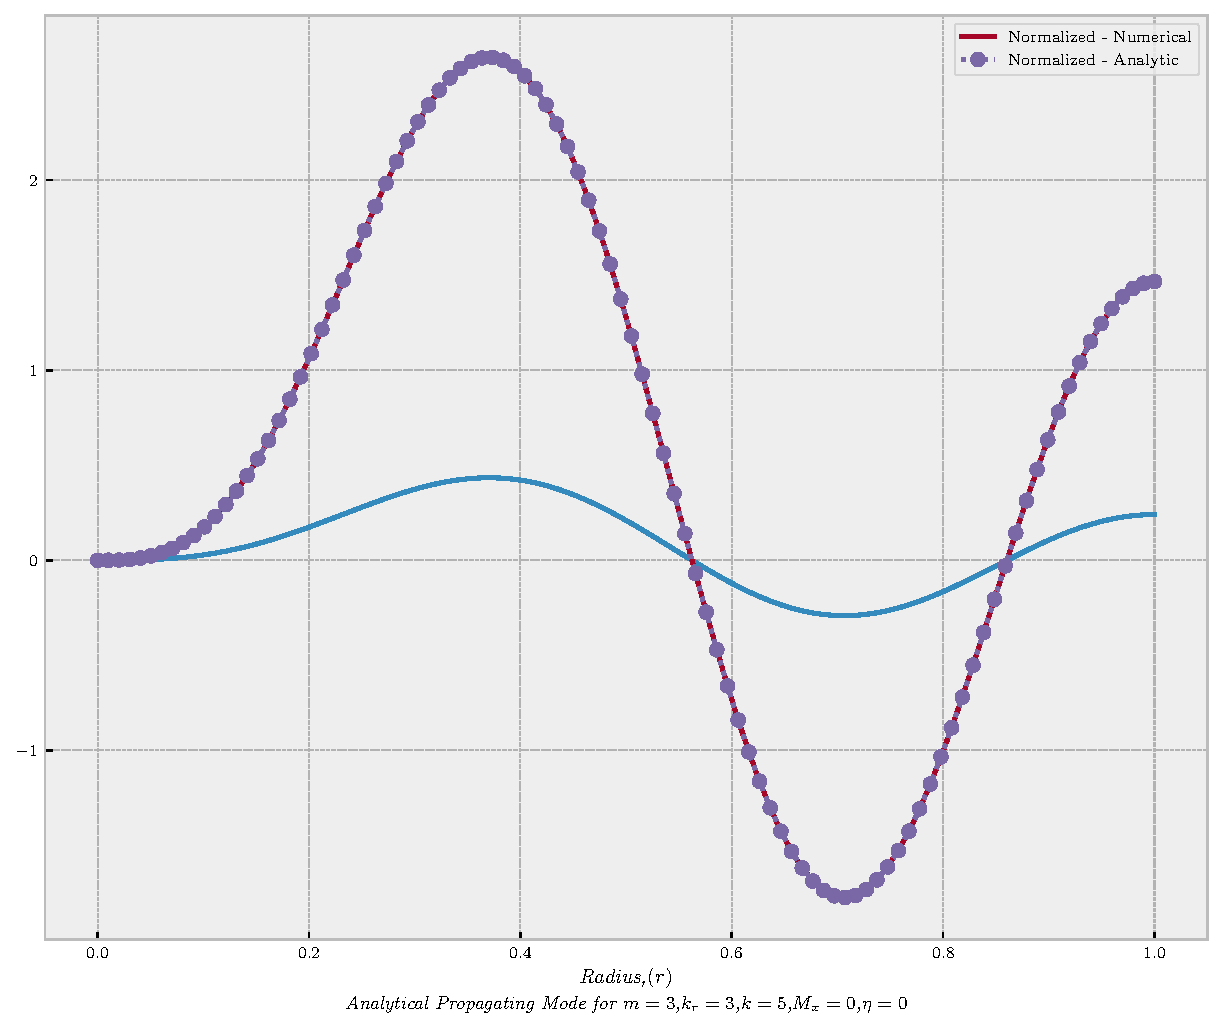
\includegraphics[width=0.5\textwidth]{Radial_mode_analytical_test_case.pdf}
    \end{figure}
\end{frame}
\begin{frame}
    \begin{figure}[!]
        \centering
        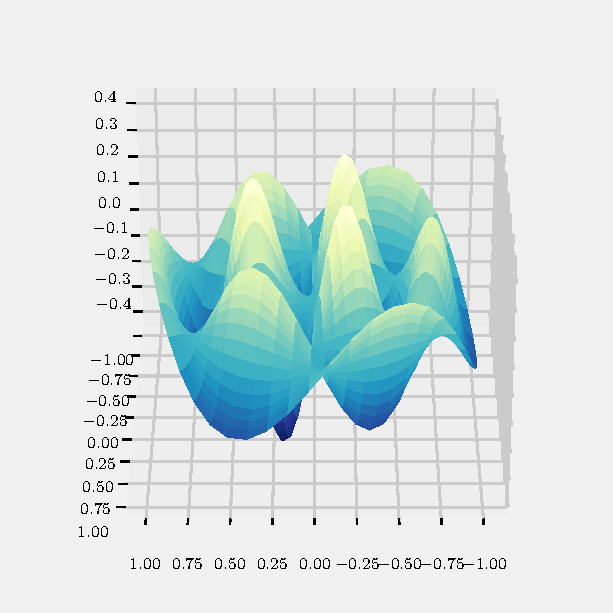
\includegraphics{Radial_mode_analytical_test_case_3d1.pdf}
    \end{figure}
\end{frame}
\begin{frame}
    \begin{figure}[!]
        \centering
        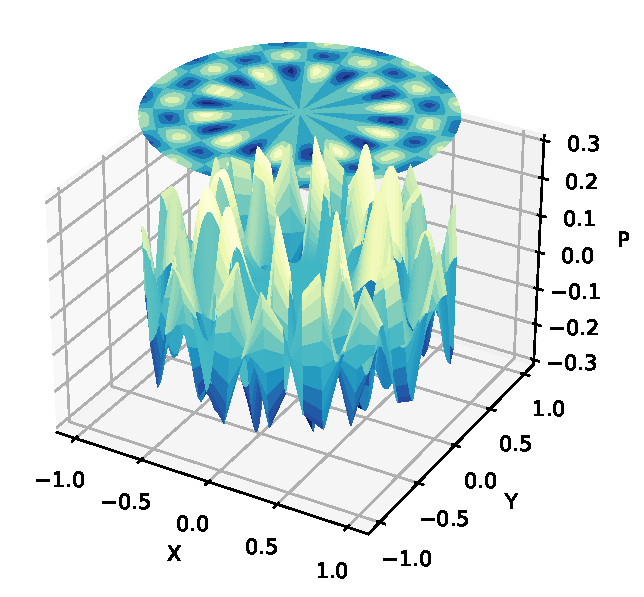
\includegraphics{Radial_mode_analytical_test_case_3d2.pdf}
    \end{figure}
\end{frame}

\begin{frame}
    \begin{figure}[!]
        \centering
        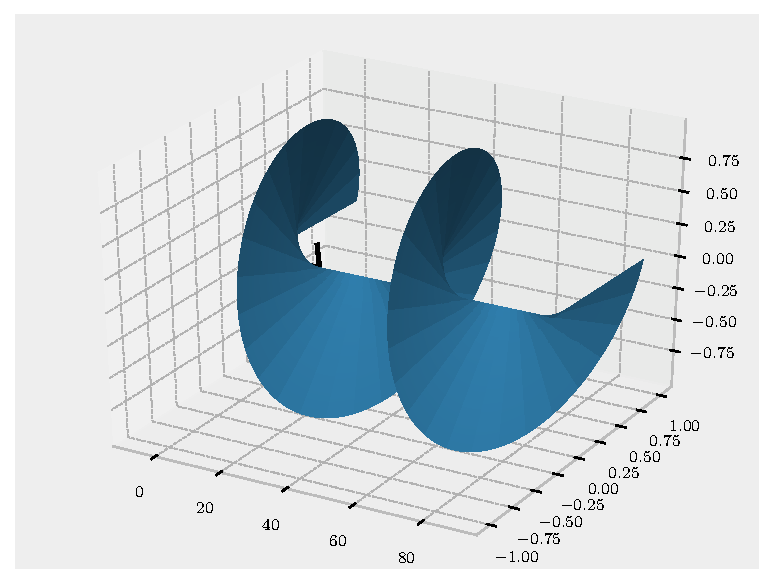
\includegraphics{helicoid_test_case_3d2.pdf}
    \end{figure}
\end{frame}
% \section{Results Update}
% \frame{\sectionpage}

% \begin{frame}{Motivation}
%     \begin{alertblock}{How is the analytical solution computed for Sound Prop. in Uniform Axial Flow}
%     \begin{enumerate}[<+->]\itemsep9pt
%         \item The analytical solution are the axial wavenumbers and propagating
%             modes for a given frequency, axial velocity and azimuthal mode order.
%         \item For a given azimuthal mode, there is a range of radial modes.
%         \item These radial modes can be categorized based on the sign of the axial wavenumber and if it is
%             complex in value. 
%         \item Propagating modes are defined by axial wavenumbers, $k_x$, that have a real-part only, yielding 
%             the assumed fluctuation to resemble Euler's Formula ($e^{ik_x x}$). 
%         \item On the other hand, if the $k_x$ is complex, then the mode will resemble an exponentially decaying
%             function since the imaginary number cancels, leaving a minus sign in front of
%             the axial wavenumber.
%     \end{enumerate}
%     \end{alertblock}

%     \tiny
%     % \hspace{3.75em}\url{http://www.klimaschutzplan2050.de/en/action-areas/energy-sector/}
% \end{frame}
% \begin{frame}

% \begin{equation}
%     k_x  = \frac{- M_x k \pm \sqrt{k^2 - ( 1 - M_x^2) J_{m,n}'^2 }}{\left( 1 - M_x^2 \right)}.
%     \label{eqn:ax_wavenumb}
% \end{equation}

% where $M_x$ is the axial Mach number, $k$ is the temporal (referred to as reduced)
% frequency, and $J_{m,n}'$ is the derivative of the Bessel function of the first kind.  
% The $\pm$ accounts for both upstream and downstream modes.

% The condition for propagation is such that the axial wavenumber is larger than 
% a ``cut-off'' value

% \begin{equation}
%     k_{x,real}  = \frac{\pm M_x k }{\left( M_x^2 - 1 \right)}.
%     \label{eqn:cuton}
% \end{equation}


% \end{frame}
% \begin{frame}
    
% Every term that is being raised to the one half i.e. square rooted must 
% be larger than zero to keep axial wavenumber from being imaginary. The mode 
% will propagate or decay based on this condition. Recall thaT the mode is of the 
% form 
% \begin{equation}
%     e^{i k_x x}
%     \label{eqn:fluctuationexample}
% \end{equation}
% if $k_x$ has a real part, $k_{x,real}$ and an imaginary part $i k_{x,imag}$ 
% then,

% \begin{align}
%     &= e^{i k_x x} \\
%     &= e^{i (k_{x,real}+ i k_{x,imag}) x} \\
%     &= \underbrace{e^{i k_{x,real}x}}_{\textit{amplitude}} \underbrace{e^{- k_{x,imag} x}}_{\textit{exponential decay}} 
% \end{align}


% \end{frame}
% \begin{frame}
    

% Although the ``cut-off'' decay to nearly zero rapidly, the rate at which this occured
% was not much of a concern earlier on in turbomachinery design. As nacelles 
% continue to grow shorter, a mode that is ``cut-off'' may make it outside the duct.

% For this work a desired amplitude was arbitrarily chosen for a mode, $y_{desired}$
% and then the axial location at which this occurred, $x_{desired}$ which 
% can be compared against a desired length for a nacelle.  
% Since SWIRL assumes an infinitely long duct, there is nothing limiting the 
% modes propagation with respect to nacelle length. For example, if the 
% desired amplitude is one percent, then $x_{desired}$,

% \begin{align*}
%     0.01 &=  e^{-10 x_{desired}},\\
%     -\frac{ln|0.01|}{10} &=  x_{desired},\\
%     -\frac{ln|0.01|}{10} &= 0.4605170185988091 .
% \end{align*}

% \end{frame}
% \begin{frame}
    


%  \begin{figure}
%      \centering
%      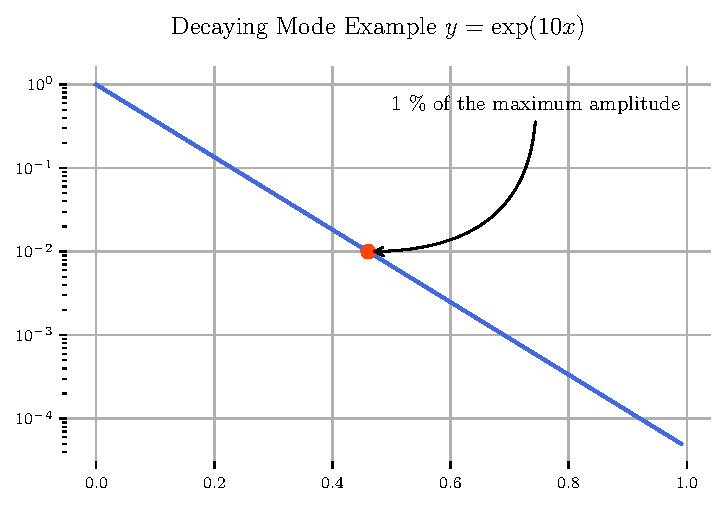
\includegraphics[width=0.7\textwidth]{/home/jeff-severino/SWIRL/CodeRun/04-plotReport/tex-outputs/desired_cut_off_location_1_percent_of_max2.pdf}
%      \caption{Decaying mode with $k_x = 0 + 10j$ and unit amplitude. One percent
%      of the maximum amplitude is identified for nacelle length comparison}
%      \label{fig:decaying_mode_with_1_percent_amp}
%  \end{figure}
 
 
% In general,
% \begin{align*}
%     y_{desired} &=  e^{-k_{x,imag} x_{desired} }\\
%     -\frac{ln|y_{desired}|}{k_{x,imag}} &=  x_{desired}
% \end{align*}
% \end{frame}
% \begin{frame}
% \section{Analytical Test Case 1}
% \begin{table}[h!]
%     \centering
%     \begin{tabular}{|l|l|}
%         \hline
%         $\sigma$ & \textit{0.0} \\ \hline
%         $k$      & \textit{10}   \\ \hline
%         $m$      & \textit{2}    \\ \hline
%         $M_x$    & \textit{0.3}  \\ \hline
%     \end{tabular}
%     \caption{Validation test case parameters, Uniform Flow Annular Duct} 
% \end{table}

% \end{frame}

% \begin{frame}
    
%  \begin{figure}
%      \centering
%      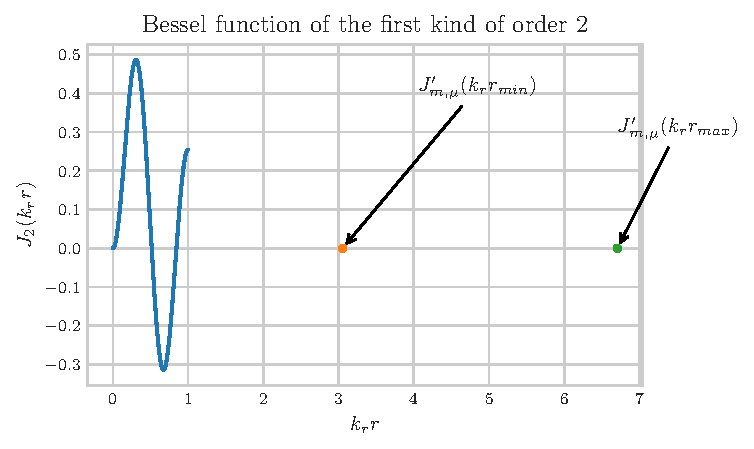
\includegraphics[width=0.7\textwidth]{/home/jeff-severino/SWIRL/CodeRun/04-plotReport/tex-outputs/bessel_analytical_test_case.pdf}
%      \caption{The Bessel function with the values of $J'_{m,\mu}$ labeled}
%      \label{fig:decaying_mode_with_1_percent_amp}
%  \end{figure}
% \end{frame}



% \begin{frame}
    
%  \begin{figure}
%      \centering
%      \includegraphics[width=0.7\textwidth]{/home/jeff-severino/SWIRL/CodeRun/04-plotReport/tex-outputs/axial_wavenumber_analytical_test_case.pdf}
%      \caption{The Bessel function with the values of $J'_{m,\mu}$ labeled}
%      \label{fig:decaying_mode_with_1_percent_amp}
%  \end{figure}
% \end{frame}


% \begin{frame}{Normalized Mode}

    
%  \begin{figure}
%      \centering
%      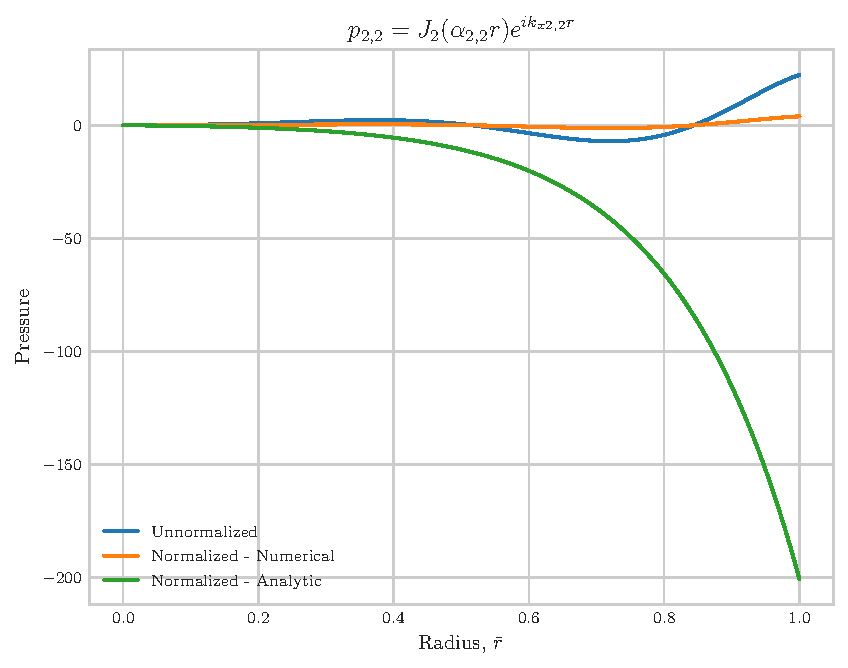
\includegraphics[width=0.7\textwidth]{/home/jeff-severino/SWIRL/CodeRun/04-plotReport/tex-outputs/Normalized_Mode_test_case.pdf}
%      \caption{The Bessel function with the values of $J'_{m,\mu}$ labeled}
%      \label{fig:decaying_mode_with_1_percent_amp}
%  \end{figure}
% \end{frame}
% \begin{frame}
    
% \end{frame}




% \begin{frame}{Future Work}
%     \begin{alertblock}{}
%     \begin{enumerate}[<+->]\itemsep9pt
%         \item I need to use sanity checks to ensure that the normalization provided
%             by Rienstra is implemented correctly.
%         \item While the numerical normalized mode has an integral of one, the 
%             analytical mode is not.
%         \item a few things that have been checked along the way but need to be 
%             reported are,
%         \item Zero's of $J'_m$ 
%         \item Value of $J_m$ at the zero location
%         \item Relations involving integrals If it so not too cumbersome.
%             There are some simplifications that could be checked\ldots 
%         \item Check the analytical test case that has been reported in literature.
%            The difference is that $\sigma = 0.25$
%     \end{enumerate}
%     \end{alertblock}

%     \tiny
%     % \hspace{3.75em}\url{http://www.klimaschutzplan2050.de/en/action-areas/energy-sector/}
% \end{frame}

% % \begin{frame}{Perspective}{Disciplines for investigating energy topics}
% %     \begin{center}
% %     \begin{tikzpicture}[
% %       node distance=4.5em and .75cm,font=\small
% %     ]
% %     % flowboxes
% %     \node[flowbox] (physik) {
% %         \fbtitle{Physics}\vphantom{yÖ}
% %     \nodepart{two}
% %         \begin{minipage}{.16\textwidth}
% %             \centering
% %             Theoretical\\ feasibility\\
% %             \scriptsize (Natural laws)
% %         \end{minipage}
% %     };

% %     \node[flowbox,right=of physik] (technik) {
% %         \fbtitle{Engineering}\vphantom{yÖ}
% %     \nodepart{two}
% %         \begin{minipage}{.16\textwidth}
% %             \centering
% %             Technical\\ feasibility\\
% %             \scriptsize (Technologies)
% %         \end{minipage}
% %     };

% %     \node[flowbox,right=of technik] (econ) {
% %         \fbtitle{Economy}\vphantom{yÖ}
% %     \nodepart{two}
% %         \begin{minipage}{.16\textwidth}
% %             \centering
% %             Economic\\ feasibility\\
% %             \scriptsize (Funding)
% %         \end{minipage}
% %     };

% %     \node[flowbox,right=of econ] (society) {
% %         \fbtitle{Society}\vphantom{yÖ}
% %     \nodepart{two}
% %         \begin{minipage}{.16\textwidth}
% %             \centering
% %             Social\\ feasibility\\
% %             \scriptsize (Decision space)
% %         \end{minipage}
% %     };

% %     \uncover<2->{%
% %         \draw [decorate,decoration={brace,amplitude=10pt,mirror},ultra thick,jdblue]
% %             ($(technik.south west) + (-.2em,-1em)$) --
% %             ($(econ.south east)    + (+.2em,-1em)$) coordinate[midway,yshift=-3.8em] (midpoint-below);
    
% %         \node[flowbox] at (midpoint-below) (tech-econ)  {
% %             \fbtitle{Techno-economic modelling}\vphantom{yÖ}
% %         \nodepart{two}
% %             \begin{minipage}{.4\textwidth}
% %                 \centering
% %                 How much energy?
% %                 For how much?\vphantom{yÖ}
% %             \end{minipage}
% %         };
% %     }
% %     \end{tikzpicture}
% %     \end{center}
% % \end{frame}


\subsection{Theory}

To relate the speed of sound to a given flow, the radial momentum equation
is used.  If the flow contains a swirling component,then the primitive variables 
are nonuniform through the flow, and mean flow assumptions are not valid. 
\begin{align*}
    \frac{\partial v_r}{\partial t} +
    v_r \frac{\partial v_r}{\partial r} + 
    \frac{v_{\theta}}{r} 
    \frac{\partial v_{\theta}}{\partial \theta} -
    \frac{v_{\theta}^2}{r} 
    v_x \frac{\partial v_r}{\partial x} =
    \frac{1}{\rho}\frac{\partial P}{\partial r}
\end{align*}

 To account to for this, the radial momentum is simplified by assuming the 
 flow is steady, the flow has no radial component. In addition, the viscous
 and body forces are neglected.  Then the radial pressure derivative term is
 set equal to the dynamic pressure term. Seperation of variables is applied.  

 \begin{align*}
     \frac{v_{\theta}^2}{r} = \frac{1}{\rho}\frac{\partial P}{\partial r} \\
 P = \int_{r}^{r_{max}} \frac{\rho V_{\theta}^2}{  r}
 \end{align*}

To show the work, we will start with the dimensional form of the equation and
differentiate both sides.  Applying separation of variables,
 \[
     \int_{r}^{r_{max}}
     \frac{\bar{\rho} v_{\theta}^2}{r} \partial r 
     =-\int_{P(r)}^{P(r_{max})}\partial p.
 \]

Since $\tilde{r} = r/r_{max}$,
\[r = \tilde{r}r_{max}.\]
Taking total derivatives (i.e. applying chain rule),
\[dr = d(\tilde{r}r_{max}) = d(\tilde{r})r_{max}, \]
Substituting these back in and evaluating the right hand side,
\[
    \int_{\tilde{r}}^{1} \frac{\bar{\rho} v_{\theta}^2}{\tilde{r}}\partial \tilde{r} 
    =P(1)-P(\tilde{r})
\]

For reference the minimum value of $\tilde{r}$ is,

\[\sigma = \frac{r_{max}}{r_{min}}\]

For the radial derivative, the definition of the speed of sound is utilized,
\[\frac{\partial A^2}{\partial r } =
\frac{\partial}{\partial r} \left( \frac{\gamma P}{\rho} \right).\]

Using the quotient rule, the definition of the speed of sound is extracted,

\begin{align*}
&= \frac{\partial P}{\partial r} \frac{\gamma \bar{\rho}}{\bar{\rho}^2} -
\left(
    \frac{\gamma P}{\bar{\rho}^2} 
\right) 
\frac{\partial \bar{\rho}}{\partial r}\\
&=  \frac{\partial P}{\partial r} \frac{\gamma }{\bar{\rho}} -
\left( \frac{A^2}{\bar{\rho}} \right) 
\frac{\partial \bar{\rho} }{\partial r}
\end{align*}

Using isentropic condition $ \partial P/A^2 = \partial \rho$, 

\begin{align*}
&= \frac{\partial P}{\partial r} \frac{\gamma }{\bar{\rho}} -
\left( \frac{1}{\bar{\rho}} \right) \frac{\partial  P }{\partial r}\\
\frac{\partial A^2}{\partial r} 
&= \frac{\partial P}{\partial r} \frac{\gamma - 1}{\bar{\rho}}  
\end{align*}

\begin{align*}
    \frac{\bar{\rho}}{\gamma -1}\frac{\partial A^2}{\partial r} &= \frac{\partial P}{\partial r} 
\end{align*}


Going back to the radial momentum equation, and rearranging the terms will simplify 
the expression. The following terms are defined to start the
nondimensionalization.  

\begin{align*}
    M_{\theta} &= \frac{V_{\theta}}{A} \\ 
    \widetilde{r} &= \frac{r}{r_{max}}  \\
    \widetilde{A} &= \frac{A}{A_{r,max}}  \\
    A &= \widetilde{A}{A_{r,max}} \\
    r &= \widetilde{r}{r_{max}}\\
    \frac{\partial}{\partial r} &=
    \frac{\partial \widetilde{r}}{\partial r} \frac{\partial}{\partial \widetilde{r}}\\
                                &= \frac{1}{r_{max}}\frac{\partial}{\partial \widetilde{r}}
\end{align*}
Dividing by $A$,
\begin{align*}
    \frac{M_{\theta}^2}{r}\left(\gamma - 1\right) 
 &= \frac{\partial A^2}{\partial r} \frac{1}{A^2}
\end{align*}

Now there is two options, either find the derivative of  $\bar{A}$ or the integral of
$M_{\theta}$ with respect to r.
\begin{enumerate}
    \item
%\begin{align*}
%\text{Integrating both sides } 
%\int_{r}^{r_{max}}\frac{M_{\theta}}{r}\left(\gamma - 1\right){\partial r}  &=\int_{A^2(r)}^{A^2(r_{max})}\frac{1}{A^2}  {\partial A^2}\\
%\int_{r}^{r_{max}}\frac{M^2_{\theta}}{r}\left(\gamma - 1\right){\partial r}  &=ln(A^2(r_{max})) - ln(A^2(r)) \\
%\int_{r}^{r_{max}}\frac{M^2_{\theta}}{r}\left(\gamma - 1\right){\partial r}  &=ln\left(\frac{A^2(r_{max})}{A^2(r)}\right) 
%\end{align*}
%
Defining non dimensional speed of sound $\tilde{A} = \frac{A(r)}{A(r_{max})}$
\begin{align*}
\int_{r}^{r_{max}}\frac{M_{\theta}}{r}\left(\gamma - 1\right){\partial r}  &=ln\left(\frac{1}{\tilde{A}^2}\right) \\
&= -2ln(\tilde{A})\\
\tilde{A}(r) &= exp\left[-\int_{r}^{r_{max}}\frac{M_{\theta}}{r}\frac{\left(\gamma - 1\right)}{2}{\partial r}\right] \\ \text{replacing r with }\tilde{r} \rightarrow \tilde{A}(r) &= exp\left[-\int_{r}^{r_{max}}\frac{M_{\theta}}{r}\frac{\left(\gamma - 1\right)}{2}{\partial r}\right]		\\
\tilde{A}(\tilde{r}) &= exp\left[\left(\frac{1 - \gamma}{2}\right)\int_{\tilde{r}}^{1}\frac{M_{\theta}}{\tilde{r}}{\partial \tilde{r}}\right]	
\end{align*}
\item Or we can differentiate
\end{enumerate}
Solving for $M_{\theta}$ ,
\begin{align*}
M_{\theta}^2 
&= \frac{\partial A^2}{\partial r} \frac{r}{A^2 \left(\gamma - 1\right)}
\end{align*}
Nondimensionalizing and substituting, 

\begin{align} 
    M_{\theta}^2
    \frac{\left( \gamma - 1 \right)}{\widetilde{r} r_{max}} &=
    \frac{1}{(\widetilde{A}A_{r,max})^2}\frac{A_{r,max}^2}{r_{max}}
    \frac{\partial \widetilde{A}^2}{\partial \widetilde{r}} \nonumber \\
    M_{\theta}^2     \frac{\left( \gamma - 1 \right)}{\widetilde{r} } &=
    \frac{1}{\widetilde{A}^2}
    \frac{\partial \widetilde{A}^2}{\partial \widetilde{r}} \nonumber \\
    M_{\theta} &= \sqrt{\frac{\widetilde{r}}{(\gamma-1) \widetilde{A}^2}
        \frac{\partial\widetilde{A}^2}{\partial \widetilde{r} }
    } \label{eq:Mthetabackcalculated}
\end{align}

% 3.1 Guidelines for Creating Manufactured Solutions states:
% \begin{enumerate}
%     \item  The manufactured solutions should be composed of smooth analytic 
%         functions 
%     \item The manufactured solutions should exercize every term in the governing
%         equation that is being tested,
%     \item The solution should have non trivial derivatives.  
%     \item The solution derivatives should be bounded by a small constant. In this case
%         this constant should prevent the function from becoming greater than 
%         one.
%     \item The solution should not prevent the code from running 
%     \item The solution should be defined on a connected subset of two- or three-
%         dimensional space to allow flexibility in chosing the domain of the PDE.
%         Section 3.3.1 provides more information about this.
%     \item The solution should coincide with the differential operators of the PDE.
%         For example, the flux term in Fourier's law of conduction requires T to 
%         be differentiable.
% \end{enumerate}
% With these guidelines, a function is specified for the speed of sound to conduct
% a method of manufactured solutions on SWIRL's speed of sound numerical 
% integration. This is checked by observing the tangential mach number 
% produced from the speed of sound and comparing that to the tangential mach number
% that has been analytically defined (See Equation \ref{eq:Mthetabackcalculated}).


\subsection{Procedure}
There are a few constraints and conditions that must be followed in order for the analytical 
function to work with SWIRL, 

\begin{itemize}
    \item The mean flow and speed of sound must be real and positive. This will 
        occur is a speed of sound is chosen such that the tangential mach number
        is imaginary
    \item The derivative of the speed of sound must be positive
    \item Any bounding constants used with the mean flow should not allow the 
        total Mach number to exceed one.
    \item the speed of sound should be one at the outer radius of the cylinder
\end{itemize}

Given these constraints, $tanh(r)$ is chosen as a function since it can be
modified to meet the conditions above. Literature (The tanh method: A tool for 
solving certain classes of nonlinear evolution and wave equations) 
is a paper than demonstrates the strength of using tanh functions.
One additonal benefit of tanh(r) is that it is bounded between one and negative one, i.e.

\begin{itemize}
    \item As r $\rightarrow$ $\infty$ tanh(r) $\rightarrow$ 1
    \item As -r $\rightarrow$ $-\infty$ tanh(r) $\rightarrow$ -1
\end{itemize}

To test the numerical integration method,  $M_{\theta}$ is defined as a result 
of differentiating the speed of sound, $A$. This is done opposed to integrating
$M_{\theta}$ analytically. However, an analytical function can be defined for
$M_{\theta}$, which can then be integrated to find what $\widetilde{A}$ should be. 
Instead, the procedure of choice is to back calculate what the appropriate 
$M_{\theta}$ is for a given expression for $\widetilde{A}$.  Since it is easier 
to take derivatives , we will solve for $M_{\theta}$ using Equation \ref{eq:Mthetabackcalculated} ,

\subsection{Tanh Summaion Formulation}
Knupp's Code Verification by the Method of Manufactured Solution (MMS) provides 
``guidelines'' for creating a manufactured solution (MS) such that the observed
order of accuracy will approach a theoretical order of accuracy as the number
of grid points are reduced from one iteration to the next. While these guidelines
offer a road map, there are choices that are left to the investigator that would
benefit from additional examples. The first guideline gives the user a free
choice of the MS as long as it s smooth. The benefit of the tanh summation method 
(TSM) reduces the difficuly in defining a sufficient MS by providing 
a general summation formulation that allows the user to Vary the number of 
terms in the MS, and the MS behavior without manually changing terms in the MS
symbolic expression. 

The general form of the MS will be a summation of $tanh$ bounded between zero
and one. A MS created with the TSM can provide a significant result for
a numerical differencing/integration technique by having inflection points of each
$tanh$ at various locations along the domain, giving a stair like slope.
While the TSM can add a layer of complexity to the MS that may not be needed, 
writing the formulation in a summation lends itself to iterative loops that can 
be coded, thus reducing the need for manual adjust of the MS, 
which can be an initial hurdle when performing MMS.


\section{General form of a Hyperbolic Tangent}

\begin{equation}
    R = A tanh(B(x-C)) 
    \label{eqn:1}
\end{equation}

\begin{equation}
    L = A tanh(B(C-E)) 
    \label{eqn:2}
\end{equation}
\begin{equation}
    y = R + L + D
    \label{eqn:3}
\end{equation}
where 
\begin{itemize}
    \item $R \equiv$ The value of the hyperbolic tangent. The variable $R$ represnts
        a ``right'' facing hyperbolic tangent kink.
    \item $A \equiv$ magnitude factor that increases or decreases the asymptotic
        limits $\lim_{x \to -\infty} = -1$ $\lim_{x \to \infty} = 1$
    \item $B \equiv$ ``steepness'' of the hyperbolic tangent
    \item $C \equiv$ The shift in inflection point of the hyperbolic tangent along the $
        x$ axis 
    \item $D \equiv$ The shift in inflection point of the hyperbolic tangent along the $
        y$ axis 
    \item $E \equiv$  $x_{i=i_{max}}$
    \item $x$ The domain. $x_i$ is used to indicate grid point indicies.
\end{itemize}
The idea is to sum up an arbitrary amount of tangents that will be bounded by zero
and one. 

\begin{figure}
    \centering
    \resizebox{\columnwidth}{!}{
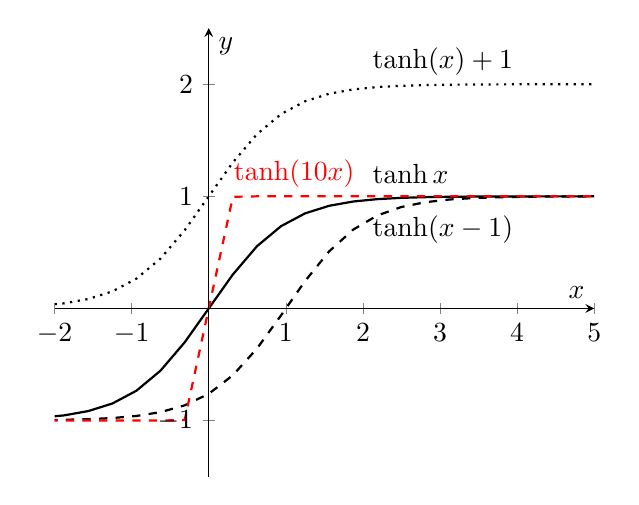
\begin{tikzpicture}
    \begin{axis}[
        xmin=-2, xmax=5,
        ymin=-1.5, ymax=2.5,
        axis lines=center,
        axis on top=true,
        domain=-2.5:5,
        ylabel=$y$,
        xlabel=$x$,
        ]

        \addplot [mark=none,draw= black, thick] {tanh(\x)};
        \node [right, black ] at (axis cs: 2,1.2) {$ \tanh x$};


        \addplot [mark=none,draw=black, dashed, thick] {tanh(\x - 1)};
        \node [right, black] at (axis cs: 2,0.7) {$ \tanh (x - 1)$};



        \addplot [mark=none,draw=red, dashed, thick] {tanh(10*\x)};
        \node [right, red] at (axis cs: 0.2,1.2) {$ \tanh (10x )$};



        \addplot [mark=none,draw=black, dotted, thick] {tanh(\x) + 1};
        \node [right, black] at (axis cs: 2,2.2) {$ \tanh (x) + 1$};

    \end{axis}
\end{tikzpicture}}
\end{figure}


Now the goal is to generalize this formulation such that we can add up terms.
$A$ is determined by setting a maximum amplitude for each $tanh$ function by
$A = A_{max}/n$. Note that amplitude can be different for each term but is chosen
to be the same. A parameter $\hat{x} = (x - x_{min})/ (x_{max} - x_{min}$ scales the domain to be between the  
minimum and maximum bounds.


\begin{equation}
    R_{ij} = A tanh(B(x_i-C_j)) 
    \label{eqn:1}
\end{equation}

\begin{equation}
    L_{j} = A tanh(B(C_j-E)) 
    \label{eqn:2}
\end{equation}
\begin{equation}
    y = \sum_{j = 1}^{n}  R_{ij} + \sum_{j = 1}^{n}L + D
    \label{eqn:3}
\end{equation}
The function \verb|TanhMethod| does this procedure. 

Setting $A = 1/16$ and $C_1  = 0$ , $C_2 = 0.75$ , $C_3 = 1$ , $D = 1$, $E = 1$  and 
$B = 10$


\begin{equation}
    \sum_{j = 1}^{3} R_{ij} = 1/16 tanh(10(\hat{x}_i))  + 1/16 tanh(10(\hat{x}_i-0.75)) + 1/16 tanh(10(\hat{x}_i-1))
    \label{eqn:1}
\end{equation}

\begin{equation}
    \sum_{j = 1}^{3} L_{j} = 1/16 tanh(10(-1))  + 1/16 tanh(10(0.75 - 1)) + 1/16 tanh(10(1-1))
    \label{eqn:1}
\end{equation}

The simplified expression becomes,
\begin{equation}
    y = \frac{1}{16}\tanh\left(\frac{100}{9}r - \frac{100}{9}\right) + \frac{1}{16}\tanh\left(\frac{100}{9}r -\frac{55}{9}\right) + \frac{1}{16}\tanh\left(\frac{100}{9}r -\frac{10}{9} \right) + \frac{7}{8}
\end{equation}


%\begin{figure}
%    \centering
%    \resizebox{\columnwidth}{!}{
%% This file was created with tikzplotlib v0.10.1.
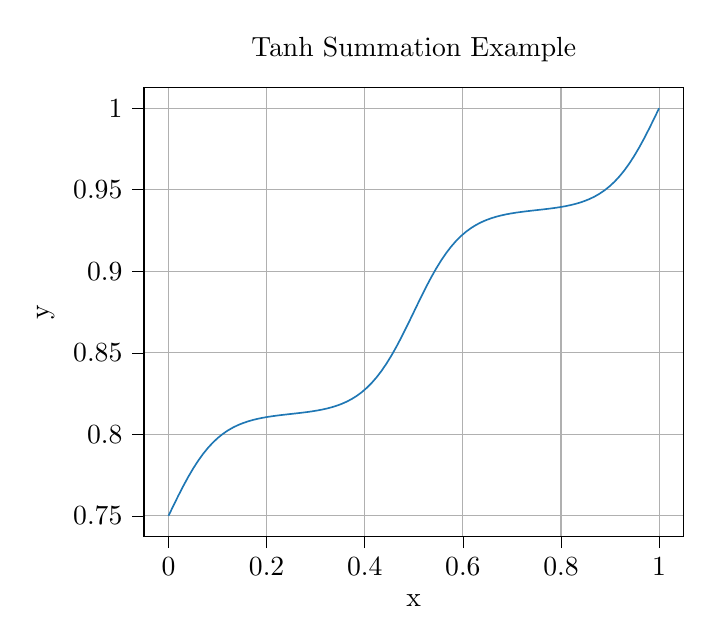
\begin{tikzpicture}

\definecolor{darkgray176}{RGB}{176,176,176}
\definecolor{steelblue31119180}{RGB}{31,119,180}

\begin{axis}[
tick align=outside,
tick pos=left,
title={Tanh Summation Example},
x grid style={darkgray176},
xlabel={x},
xmajorgrids,
xmin=-0.05, xmax=1.05,
xtick style={color=black},
y grid style={darkgray176},
ylabel={y},
ymajorgrids,
ymin=0.737511917481587, ymax=1.01249943250088,
ytick style={color=black}
]
\addplot [semithick, steelblue31119180]
table {%
0 0.750011349982464
0.0101010101010101 0.756304367923548
0.0202020202020202 0.762471427961815
0.0303030303030303 0.768396284241735
0.0404040404040404 0.773980954849054
0.0505050505050505 0.779151246168556
0.0606060606060606 0.78385900159005
0.0707070707070707 0.788081304133098
0.0808080808080808 0.791817372304981
0.0909090909090909 0.795084105493723
0.101010101010101 0.797911187966577
0.111111111111111 0.80033644822293
0.121212121212121 0.802401902498815
0.131313131313131 0.804150668035091
0.141414141414141 0.805624753143957
0.151515151515152 0.806863623924088
0.161616161616162 0.807903399550648
0.171717171717172 0.808776520778204
0.181818181818182 0.809511752175423
0.191919191919192 0.810134404577104
0.202020202020202 0.810666691986701
0.212121212121212 0.811128162249061
0.222222222222222 0.811536161419119
0.232323232323232 0.81190630759737
0.242424242424242 0.812252961565677
0.252525252525253 0.812589689584715
0.262626262626263 0.812929718947268
0.272727272727273 0.813286389915873
0.282828282828283 0.813673608902656
0.292929292929293 0.814106307344292
0.303030303030303 0.814600908628971
0.313131313131313 0.815175801361504
0.323232323232323 0.815851810708233
0.333333333333333 0.816652649865894
0.343434343434343 0.817605320080265
0.353535353535354 0.81874040944222
0.363636363636364 0.820092217733837
0.373737373737374 0.82169860781786
0.383838383838384 0.82360045643945
0.393939393939394 0.825840555061835
0.404040404040404 0.828461805118854
0.414141414141414 0.831504577298413
0.424242424242424 0.835003179865009
0.434343434343434 0.838981523240156
0.444444444444444 0.84344828154901
0.454545454545455 0.848392114910775
0.464646464646465 0.853777768834061
0.474747474747475 0.859544011154561
0.484848484848485 0.865604291561671
0.494949494949495 0.871850642171087
0.505050505050505 0.878160707811378
0.515151515151515 0.884407058420794
0.525252525252525 0.890467338827903
0.535353535353535 0.896233581148403
0.545454545454546 0.901619235071689
0.555555555555556 0.906563068433454
0.565656565656566 0.911029826742308
0.575757575757576 0.915008170117455
0.585858585858586 0.918506772684051
0.595959595959596 0.92154954486361
0.606060606060606 0.924170794920629
0.616161616161616 0.926410893543014
0.626262626262626 0.928312742164604
0.636363636363636 0.929919132248627
0.646464646464647 0.931270940540244
0.656565656565657 0.9324060299022
0.666666666666667 0.93335870011657
0.676767676767677 0.934159539274231
0.686868686868687 0.93483554862096
0.696969696969697 0.935410441353493
0.707070707070707 0.935905042638172
0.717171717171717 0.936337741079808
0.727272727272727 0.936724960066591
0.737373737373737 0.937081631035197
0.747474747474748 0.937421660397749
0.757575757575758 0.937758388416787
0.767676767676768 0.938105042385094
0.777777777777778 0.938475188563345
0.787878787878788 0.938883187733403
0.797979797979798 0.939344657995763
0.808080808080808 0.939876945405361
0.818181818181818 0.940499597807041
0.828282828282828 0.94123482920426
0.838383838383838 0.942107950431816
0.848484848484849 0.943147726058376
0.858585858585859 0.944386596838507
0.868686868686869 0.945860681947373
0.878787878787879 0.947609447483649
0.888888888888889 0.949674901759534
0.898989898989899 0.952100162015887
0.909090909090909 0.954927244488741
0.919191919191919 0.958193977677483
0.929292929292929 0.961930045849366
0.939393939393939 0.966152348392414
0.94949494949495 0.970860103813909
0.95959595959596 0.97603039513341
0.96969696969697 0.981615065740729
0.97979797979798 0.98753992202065
0.98989898989899 0.993706982058916
1 1
};
\end{axis}

\end{tikzpicture}

%}
%\end{figure}
%The goal is generate an MS with a number of ``stairs'' that is bounded between
%zero and one. Here's what my focus group ideas are,
%
%\begin{align*}
%    1 = R + L 
%\end{align*}
%where, 1 is a constraint, and R and L are the two waves when summed need to cancel 
%if it were the exact same amplitude \& opposite sign 
%
%so ,
%
%\begin{align*}
%    R + L = \tanh(x) + -\tanh(x) = 0
%\end{align*}
%or in our case,
%
%\begin{align*}
%    R + L = \tanh(x) + -\tanh(x) = 1
%\end{align*}
%
%We can tweak this by adding knobs by adding ``knobs'' A and B. If we dont want 
%the total to not exceed one then, $A_j + A_{j+1} \cdots A_{last} = 1$. $B_1$ changes
%the steepnes of the kink that we want. In order to generalize this,
%
%
%\begin{align*}
%    \bar{A} = \sum_{j=1}^n R_{ij} + \sum_{j=1}^n L_{ij} 
%\end{align*}
%where,
%\begin{align*}
%    R_{ij} = A_j \tanh(B_j (x_i - x_j)) \\ 
%    L_{ij} = A_j \tanh(B_j (x_j - x_n))  
%\end{align*}
%
%Letting $n = 3 \ldots$
%
%\begin{align*}
%    \bar{A} &= S_{vert} + \sum_{j=1}^3 R_{ij} + \sum_{j=1}^3 L_{ij} \\
%    \bar{A} &=
%    A_1 \tanh(B_1 (x_i - x_1))  + 
%    A_{2} \tanh(B_{2} (x_i - x_{2}))  + 
%    A_{3} \tanh(B_{3} (x_i - x_3)) +  \\
%    A_1 \tanh(B_1 (x_1 - x_n)) &+ 
%    A_{2} \tanh(B_{2} (x_2 - x_{n}))  +
%    A_{3} \tanh(B_{3} (x_3 - x_n))  
%\end{align*}
%and,
%\begin{align*}
%    A_1 = A_2 = A_3 = k_1 \\ 
%    B_1 = B_2 = B_3 = k_2  
%\end{align*}
%
A tanh summation method was constructed to make a manufactured solution with 
strong changes in slope. This ensures that the numerical approximation will not 
give trivial answers. 
then for some functions we need to impose boundary conditions. We will demonstrate
how the careless implementation of a boundary condition can lead to close approximations
on the interior.  The speed of sound is defined with the subscript $analytic$ to indicate that this is the analytical function of choice and has no physical relevance 
to the actual problem.

\begin{align*}
\widetilde{A}_{analytic} = \Lambda + k_1 \tanh \left( k_2 \left( \widetilde{r} - \widetilde{r}_{max} \right) \right),
\end{align*}

where, 

\begin{align*}
    \Lambda = 1 - k_1 \tanh(k_2 (1 - \widetilde{r}_{max})),
\end{align*}

When, $\widetilde{r}=\widetilde{r}_{max}$ , $\widetilde{A}_{analytic} = 1$.  
Taking the derivative with respect to $\widetilde{r}$,

\begin{align*}
    \frac{\partial \widetilde{A}_{analytic} }{\partial \widetilde{r}} &=
    \left(1 - \tanh^{2}{\left(\left(r - r_{max}\right) {k}_{2} \right)}\right) {k}_{1} {k}_{2}, \\ 
    &= \frac{ k_{1} k_{2}}{\cosh^{2}{\left(\left(r - r_{max}\right) {k}_{2} \right)}}.
\end{align*}

Substitute this into the expression for $M_{\theta}$ in Equation 
\ref{eq:Mthetabackcalculated},

\begin{align*}
    M_{\theta} = \sqrt{2}
    \sqrt{\frac{r {k}_{1} {k}_{2}}{\left(\kappa - 1\right) \left(\tanh{\left(\left(r - r_{max}\right) {k}_{2} \right)} {k}_{1} + \tanh{\left(\left(r_{max} - 1\right) {k}_{2} \right)} {k}_{1} + 1\right) \cosh^{2}{\left(\left(r - r_{max}\right) {k}_{2} \right)}}}
\end{align*} 

Now that the mean flow is defined, the integration method used to obtain the 
speed of sound

% What happens when $r = r_{max}$?

Initially the source terms were defined without mention of the indices of the 
matrices they make up. In other words, there was no fore sight on the fact that
these source terms are sums of the elements within A,B, and X. To investigate 
the source terms in greater detail, the FORTRAN code that calls the source 
terms will output the terms within the source term and then sum them, instead 


of just their sum.
i
$ [A]{x} = \lambda [B] {x} $

which can be rearranged as,

$ [A]{x} - \lambda [B] {x} = 0$

Here, $x$ is an eigenvector composed of the perturbation variables, $v_r,v_{\theta},v_x,p$ and $\lambda$ is the associated eigenvalue, (Note: $\lambda = -i \bar{\gamma}$)

Writing this out we obtain $\cdots$.

Linear System of Equations:
\begin{equation}
    -
    i \left(
        \frac{k}{A} - \frac{m}{r} M_{\theta}
    \right)
    v_r 
    -
    \frac{2}{r} M_{\theta} v_{\theta} 
    +
    \frac{dp}{dr} 
    +
    \frac{(\kappa - 1)}{r} M_{\theta}^2 p
    -
    \lambda M_x v_r =S_1
\end{equation}

Using matrix notation,

\begin{equation}
    A_{11}
    x_1 
    -
    A_{12} x_2 
    +
    A_{14} x_4
    -
    \lambda B_{11} x_1 = S_1
\end{equation}


But $A_{14}$ and $A_{41}$ in Kousen's paper only has the derivative operator.
Since I am currntly writing the matrix out term by term and not doing the matrix 
math to obtain the symbolic expressions, I will define $A_{14}$ with $dp/dr$ 
and $A_{41}$ with $dv_r/dr$
Similarly,
\begin{align}
    A_{21} x_1 &-
    A_{22} x_2 +
    A_{24} x_4 &-
    \lambda B_{22} x_2 &= S_2 \\
    A_{31} x_1 &-
    A_{33} x_3 &-
    \lambda (B_{33} x_3 + B_{34} x_4) &= S_3\\
    A_{41} x_1 &+
    A_{42} x_2 +
    A_{44} x_4 &- 
    \lambda (B_{33} x_3 + B_{44} x_4) &= S_4
\end{align}
Now we can begin looking at the source terms, term by term. They each should also
converge at a known rate






%
\subsection{Calculation of Observed Order-of-Accuracy}
The numerical scheme used to perform the integration of the tangential velocity
will have a theoretical order-of-accuracy. To find the theoretical 
order-of-accuracy, the discretization error must first be defined. The error, 
$\epsilon$, is a function of id spacing, $\Delta r$

\[ \epsilon = \epsilon(\Delta r) \]

The discretization error in the solution should be proportional to 
$\left( \Delta r \right)^{\alpha}$ where $\alpha > 0$ is the theoretical order
for the computational method.  The error for each grid is expressed as 
\[ \epsilon_{M_{\theta}}(\Delta r) = |M_{\theta,analytic}-M_{\theta,calc}|\]
where $M_{\theta,analytic}$ is the tangential mach number that is defined from the
speed of sound we also defined and the $M_{\theta,calc}$ is the result from 
SWIRL. The $\Delta r$ is to indicate that this is a discretization error for a
specific grid spacing. Applying the same concept to to the speed of sound,

If we define this error on various grid sizes and compute $\epsilon$ for
each grid, the observed order of accuracy can be estimated and compared to
the theoretical order of accuracy. For instance, if the numerical soution
is second-order accurate and the error is converging to a value, the L2 norm of
the error will decrease by a factor of 4 for every halving of the grid cell 
size. 

Since the input variables should remain unchanged (except from minor changes 
from the Akima interpolation), the error for the axial and tangential mach 
number should be zero. As for the speed of sound, since we are using an analytic
expression for the tangential mach number, we know what the theoretical result
would be from the numerical integration technique as shown above. 
Similarly we define the discretization error for the speed of sound.

\[ \epsilon_{A}(\Delta r) = |A_{analytic}-A_{calc}|\]

For a perfect answer, we expect $\epsilon$ to be zero. Since a Taylor series can 
be used to derive the numerical schemes, we know that the truncation of higher
order terms is what indicates the error we expect from using a scheme that 
is constructed with such truncated Taylor series.

The error at each grid point $j$ is expected to satisfy the following,

\begin{align*}
    0 &= |A_{analytic}(r_j) - A_{calc}(r_j)| \\
    \widetilde{A}_{analytic}(r_j) &= \widetilde{A}_{calc}(r_j) +
    (\Delta r)^{\alpha} \beta(r_j)  + H.O.T
\end{align*}

where the value of $\beta(r_j)$ does not change with grid spacing, and 
$\alpha$ is the asymptotic order of accuracy of the method. It is important to
note that the numerical method recovers the original equations as the grid 
spacing approached zero.  It is important to note that $\beta$ represents the
first derivative of the Taylor Series.  Subtracting $A_{analytic}$ from both
sides gives,

\begin{align*}
    A_{calc}(r_j) - A_{analytic}(r_j) &= A_{analytic}(r_j) - A_{analytic}(r_j)
    + \beta(r_j) (\Delta r)^{\alpha} \\
    \epsilon_A(r_j)(\Delta r) &= \beta(r_j) (\Delta r)^{\alpha}
\end{align*}

To estimate the order of accuracy of the accuracy, we define the global errors 
by calculating the L2 Norm of the error which is denoted as $\hat{\epsilon}_A$ 

\begin{align*}
    \hat{\epsilon}_A = \sqrt{\frac{1}{N}\sum_{j=1}^{N} \epsilon(r_j)^2  }
\end{align*}

\begin{align*}
    \hat{\beta}_A(r_j) = \sqrt{\frac{1}{N}\sum_{j=1}^{N} \beta(r_j)^2  }
\end{align*}

As the grid density increases, $\hat{\beta}$ should asymptote to a constant 
value. Given two grid densities, $\Delta r$ and $\sigma\Delta r$, and assuming
that the leading error term is much larger than any other error term,

\begin{align*}
    \hat{\epsilon}_{grid 1} &= \hat{\epsilon}(\Delta r) = \hat{\beta}(\Delta r)^{\alpha} \\
    \hat{\epsilon}_{grid 2} &= \hat{\epsilon}(\sigma \Delta r) = \hat{\beta}(\sigma \Delta r)^{\alpha} \\
                            &= \hat{\beta}(\Delta r)^{\alpha} \sigma^{\alpha}
\end{align*}

The ratio of two errors is given by,

\begin{align*}
    \frac{\hat{\epsilon}_{grid 2}}{\hat{\epsilon}_{grid 1}} &= 
    \frac{\hat{\beta}(\Delta r )^{\alpha}}{\hat{\beta}(\Delta r )^{\alpha}} \sigma^{\alpha} \\ &= \sigma^{\alpha}
\end{align*}

Thus, $\alpha$,the asymptotic rate of convergence is computed as follows 

\begin{align*}
    \alpha = \frac{
        \ln \frac{
            \hat{\epsilon}_{grid 2}
    }{\hat{\epsilon}_{grid 1} }}
    {\ln\left( \sigma \right) }
\end{align*}

Defining  for a doubling of grid points ,
%
%\begin{align*}
%    \alpha = \frac{\ln \left( \hat{\epsilon}\left( \frac{1}{2}\Delta  r\right)
%            \right) -\ln \left( \hat{\epsilon}\left( \Delta  r\right)
%    \right)}{\ln \left( \frac{1}{2} \right)}
%\end{align*}
%
Similarly for the eigenvalue problem, 

\[ [A]x = \lambda [B]x \]


\section{Fairing Functions}
Goal: How can we modify a manufactured solution such that the endpoints are 
suitable for comparison against a codes boundary condition implementation




\section{Setting Boundary Condition Values Using a Fairing Function}

\subsection{Using $\beta$ as a scaling parameter}

Defining the nondimensional radius in the same way that SWIRL does:

\begin{align*}
    \widetilde{r} = \frac{r}{r_T}
\end{align*}
where $r_T$ is the outer radius of the annulus.

The hub-to-tip ratio is defined as:

\begin{align*}
    \sigma = \frac{r_H}{r_T}
     &= \widetilde{r}_H
\end{align*}
where $\widetilde{r}_H$ is the inner radius of the annular duct. The hub-to-tip
ratio can also be zero indicating the duct is hollow.

A useful and similar parameter is introduced, $\beta$, where $ 0 \leq \beta \leq 1$

\begin{align*}
    \beta &=
    \frac{r - r_H}{r_T - r_H}
\end{align*}
Dividing By $r_T$
\begin{align*}
    \beta &= 
    \frac{
        \frac{r}{r_T} - \frac{r_H}{r_T}
}{
        \frac{r_T}{r_T} - \frac{r_H}{r_T}
}\\
&= \frac{
    \widetilde{r} - \widetilde{r}_H
}{
1 - \sigma
}
\end{align*}

Suppose a manufactured solution $f_{MS}$ with boundaries $f_{MS}(r= \sigma)$ 
and $f_{MS}(\widetilde{r}= 1)$ is the specified analytical solution. The goal
is to change the boundary conditions of the manufactured solution in such  way 
that allows us to adequately check the boundary conditions imposed on SWIRL.
Defining the manufactured solution, $f_{MS}(\widetilde{r})$,   where
$\sigma \leq \widetilde{r} \leq 1$ and there are desired values of $f$ at the 
boundaries desired values are going to be denoted as $f_{minBC}$ and $f_{maxBC}$.
The desired changes in $f$ are defined as:

\begin{align*}
    \Delta f_{minBC} = f_{minBC} - f_{MS}(\widetilde{r} = \sigma)\\
    \Delta f_{maxBC} = f_{maxBC} - f_{MS}(\widetilde{r} = 1) 
\end{align*}
We'd like to impose these changes smoothly on the manufactured solution function.
To do this,the fairing functions, $A_{min}(\widetilde{r})$ and $A_{max}(\widetilde{r})$
where:
\begin{align*}
    f_{BCsImposed}(\widetilde{r}) = f_{MS}(\widetilde{r}) +
    A_{min}(\widetilde{r}) \Delta f_{minBC}  +  
    A_{max}(\widetilde{r}) \Delta f_{maxBC}  
\end{align*}
Then, in order to set the condition at the appropriate boundary, the following 
conditions are set,


\begin{align*}
    A_{min}(\widetilde{r} = \sigma) &= 1\\
    A_{min}(\widetilde{r} = 1) &= 0 \\
    A_{max}(\widetilde{r} = 1) &= 1 \\
    A_{max}(\widetilde{r} = \sigma) &= 0 
\end{align*}
If $A_{min}(\widetilde{r})$ is defined as a function of $A_{max}(\widetilde{r})$
then only $A_{max}(\widetilde{r})$ needs to be defined, therefore 
\begin{align*}
    A_{min}(\widetilde{r}) = 1 - A_{max}(\widetilde{r}) 
\end{align*}

It is also desirable to set the derivatives for the fairing function at the 
boundaries incase there are boundary conditions imposed on the derivatives of 
the fairing function.

\begin{align*}
    \frac{\partial A_{max}}{\partial \widetilde{r}}|_{\widetilde{r}= \sigma} &= 0\\
    \frac{\partial A_{max}}{\partial \widetilde{r}}|_{\widetilde{r}= 1} &= 0    
\end{align*}

\begin{align*}
    \frac{\partial A_{min}}{\partial \widetilde{r}}|_{\widetilde{r}= \sigma} &= 0\\
    \frac{\partial A_{min}}{\partial \widetilde{r}}|_{\widetilde{r}= 1} &= 0    
\end{align*}


\subsection{Minimum Boundary Fairing Function}

Looking at $A_{min}$ first, the polynomial is:

\begin{align*}
    A_{min} \left( \beta \right) &= 
    a + b \beta + c \beta^2 + d \beta^3                   \\
    A_{min} \left( \widetilde{r} \right) &= 
    a + b \left( \frac{\widetilde{r} - \sigma}{1 - \sigma} \right)+
    c\left( \frac{\widetilde{r} - \sigma}{1 - \sigma} \right)  ^2+
    d\left( \frac{\widetilde{r} - \sigma}{1 - \sigma} \right)^3                    \\
\end{align*}

Taking the derivative,
\begin{align*}
    A'_{min} \left( \widetilde{r} \right) &= 
    b \left( \frac{1}{1 - \sigma} \right)+
    2 c\left( \frac{1}{1 - \sigma} \right)\left( \frac{\widetilde{r} - \sigma}{1 - \sigma} \right)  +
    3 d\left( \frac{1}{1-\sigma} \right)\left( \frac{\widetilde{r} - \sigma}{1 - \sigma} \right)^2\\
    A'_{min} \left( \beta \right) &= 
    \left( \frac{1}{1 - \sigma} \right)
    \left[
    b +
    2 c \beta + 
    3 d \beta^2
    \right]
\end{align*}
Now we will use the conditons mentioned earlier as constraints to this system 
of equations
Using the possible values of $\widetilde{r}$,

\begin{align*}
    A_{min}(\sigma) &= a &= 1 \\
    A_{min}(1) &= a + b + c + d  &= 0 \\
    A'_{min}(\sigma) &=  b    &= 0 \\
    A'_{min}(1) &=  b + 2 c + 3 d    &= 0 \\
\end{align*}


which has the solution,

\begin{align*}
    a &= 1 \\
    b &= 0 \\
    c &= -3 \\
    d &= 2 
\end{align*}

giving the polynomial as: 

\begin{align*}
    A_{min} (\widetilde{r}) = 1 - 3 \left(  \frac{\widetilde{r} - \sigma }{ 1 - \sigma}\right)^2 +
    2 \left( \frac{\widetilde{r} - \sigma}{1 - \sigma} \right)^3 
\end{align*}


\subsection{Max boundary polynomial}
Following the same procedure for $A_{max}$ gives 
\begin{align*}
    A_{min} (\widetilde{r}) = 3 \left(  \frac{\widetilde{r} - \sigma }{ 1 - \sigma}\right)^2 -
    2 \left( \frac{\widetilde{r} - \sigma}{1 - \sigma} \right)^3
\end{align*}
\subsection{Corrected function} 

The corrected function is then, 

\begin{align*}
    f_{BCsImposed} (\widetilde{r}) &= 
    f_{MS}(\widetilde{r}) &+ A_{min} \Delta f_{minBC} + A_{max} \Delta f_{maxBC} \\
                                   &= 
    f_{MS}(\widetilde{r}) &+
    \left(
        1 - 3 \left(  \frac{\widetilde{r} - \sigma }{ 1 - \sigma}\right)^2 +
    2 \left( \frac{\widetilde{r} - \sigma}{1 - \sigma} \right)^3 
\right)
    \left[ \Delta f_{minBC} \right]\\ 
           & &+
    \left(
         3 \left(  \frac{\widetilde{r} - \sigma }{ 1 - \sigma}\right)^2- 
    2 \left( \frac{\widetilde{r} - \sigma}{1 - \sigma} \right)^3 
\right)
    \left[ \Delta f_{maxBC} \right] \\ 
              f_{BCsImposed} (\beta) &= f_{MS}(\beta) &+ \Delta f_{minBC} + \left(  3 \beta^2 - 2 \beta^3  \right)
    \left[  \Delta f_{maxBC} - \Delta f_{minBC} \right]
\end{align*}
Note that we're carrying the correction throughout the domain, as opposed to 
limiting the correction at a certain distance away from the boundary. The 
application of this correction ensures that there is no discontinuous derivatives
inside the domain; as suggested in Roach's MMS guidelines (insert ref) 


What is meant by ``just because $A_{min}$ and its first derivative go to zero
doesn't mean that the second derivatives''



\subsection{Symbolic Sanity Checks}
We want to ensure that $f_{BCsImposed}$ has the desired boundary conditions, 
$f_{minBC/maxBC}$ instead of the original boundary values that come along
for the ride in the manufactured solutions, $f_{MS}(\widetilde{r}=\sigma /1)$. 
In another iteration of this method, we will be changing the derivative values,
so let's check the values of $\frac{\partial f_{BCsImposed}}{\partial \widetilde{r}}$ 
to make sure those aren't effected unintentionally.

\subsubsection*{Symbolic Sanity Check 1}
The modified manufactured solution, $f_{BCsImposed}$ with the fairing functions
$A_{min}$ and $A_{max}$ substituted in is,
\begin{align*}
    f_{BCsImposed}(\widetilde{r}) =
    \left(
        3 \left(  \frac{\widetilde{r} - \sigma }{ 1 - \sigma}\right)^2- 
        2 \left( \frac{\widetilde{r} - \sigma}{1 - \sigma} \right)^3 
    \right)
    \left[ \Delta f_{maxBC} \right] .
\end{align*} 
Further simplification yields,
\begin{align*}
    f_{BCsImposed}(\widetilde{r} = \sigma) 
    &=
    \left(
        f_{MS}(\widetilde{r} = \sigma) +
        \Delta f_{minBC} +
        \left( 3\left(  \frac{\sigma - \sigma}{1 - \sigma} \right)^2- 
          2\left(  \frac{\sigma - \sigma}{1 - \sigma} \right)^3- 
        \right)
        \left[ \Delta f_{maxBC} - \Delta f_{minBC}  \right] 
    \right)\\
    &=  f_{MS}(\widetilde{r} = \sigma) + \Delta f_{minBC}\\
    &=  f_{MS}(\widetilde{r} = \sigma) + (f_{minBC} - f_{MS}(\widetilde{r} = \sigma)) \\
    &=  f_{minBC}
\end{align*} 


\begin{align*}
    f_{BCsImposed}(\widetilde{r} = 1 ) 
    &=
    \left(
        f_{MS}(\widetilde{r} = 1) +
        \Delta f_{minBC} +
        \left( 3\left(  \frac{1 - \sigma}{1 - \sigma} \right)^2- 
          2\left(  \frac{1 - \sigma}{1 - \sigma} \right)^3- 
        \right)
        \left[ \Delta f_{maxBC} - \Delta f_{minBC}  \right] 
    \right)\\
    &=  f_{MS}(\widetilde{r} = 1) + \Delta f_{maxBC}\\
    &=  f_{MS}(\widetilde{r} = 1) + (f_{maxBC} - f_{MS}(\widetilde{r} = 1)) \\
    &=  f_{maxBC}
\end{align*} 


\begin{align*}
    \frac{\partial}{\partial \widetilde{r}}\left(  f_{BCsImposed}(\widetilde{r}) =
    \left(
        3 \left(  \frac{\widetilde{r} - \sigma }{ 1 - \sigma}\right)^2- 
        2 \left( \frac{\widetilde{r} - \sigma}{1 - \sigma} \right)^3 
    \right)
    \left[ \Delta f_{maxBC} \right]\right) \\
    \frac{\partial f_{MS}}{\partial \widetilde{r}} + 
    \left( \frac{6}{1-\sigma} \right)
    \left( 
        \left( \frac{\widetilde{r} - \sigma}{1 - \sigma} \right) -
    \left( \frac{r - \sigma}{1 - \sigma} \right)^2 \right)
    \left( \Delta f_{maxBC} - \Delta f_{minBC} \right)
\end{align*} 


At $\widetilde{r} = \sigma$, the derivative is: 

\begin{align*}
    \frac{\partial f_{MS}}{\partial \widetilde{r}}|_{\sigma} \\
    \frac{\partial f_{MS}}{\partial \widetilde{r}}|_{1} 
\end{align*}


\subsection{Min boundary derivative polynomial}

The polynomial is of the form: 

\begin{align*}
    B_{min} \left( \beta \right) &= 
    a + b \beta + c \beta^2 + d \beta^3                   \\
    B_{min} \left( \widetilde{r} \right) &= 
    a + b \left( \frac{\widetilde{r} - \sigma}{1 - \sigma} \right)+
    c\left( \frac{\widetilde{r} - \sigma}{1 - \sigma} \right)  ^2+
    d\left( \frac{\widetilde{r} - \sigma}{1 - \sigma} \right)^3                    \\
\end{align*}
Taking the derivative,
\begin{align*}
    B'_{min} \left( \widetilde{r} \right) &= 
    b \left( \frac{1}{1 - \sigma} \right)+
    2 c\left( \frac{1}{1 - \sigma} \right)\left( \frac{\widetilde{r} - \sigma}{1 - \sigma} \right)  +
    3 d\left( \frac{1}{1-\sigma} \right)\left( \frac{\widetilde{r} - \sigma}{1 - \sigma} \right)^2\\
    B'_{min} \left( \beta \right) &= 
    \left( \frac{1}{1 - \sigma} \right)
    \left[
    b +
    2 c \beta + 
    3 d \beta^2
    \right]
\end{align*}


Applying the four constraints gives:
\begin{align*}
    a &= 0\\
    b &= \left( 1 - \sigma \right) \\
    a + b + c + d &= 0\\
    2 + 2c + 3d &= 0
\end{align*}
\begin{align*}
    c + d &= -b  \\
    2c + 3d &= -b
\end{align*}
\begin{align*}
    c &= -2b \\
    d &= b
\end{align*}

and the min boundary derivative polynomial is: 
\begin{align*}
    B_{min}\left( \widetilde{r} \right) &= 
    b \left( \frac{\widetilde{r} - \sigma }{1 - \sigma}\right) -
    2b\left( \frac{\widetilde{r} - \sigma }{1 - \sigma}\right) ^2 +
    b \left( \frac{\widetilde{r} - \sigma }{1 - \sigma}\right)^3 \\
    &=  \left( 1 - \sigma \right)
    \left( \left( \frac{\widetilde{r} - \sigma }{1 - \sigma}\right)  - 
    2\left( \frac{\widetilde{r} - \sigma }{1 - \sigma}\right)^2 +
    \left( \frac{\widetilde{r} - \sigma }{1 - \sigma}\right)^3\right)
\end{align*} 
\subsection{Polynomial function, max boundary derivative}
The polynomial is of the form:

The polynomial is of the form: 

\begin{align*}
    B_{max} \left( \beta \right) &= 
    a + b \beta + c \beta^2 + d \beta^3                   \\
    B_{max} \left( \widetilde{r} \right) &= 
    a + b \left( \frac{\widetilde{r} - \sigma}{1 - \sigma} \right)+
    c\left( \frac{\widetilde{r} - \sigma}{1 - \sigma} \right)  ^2+
    d\left( \frac{\widetilde{r} - \sigma}{1 - \sigma} \right)^3                    \\
\end{align*}
which has the derivative,


\begin{align*}
    B'_{max} \left( \widetilde{r} \right) &= 
    b \left( \frac{1}{1 - \sigma} \right)+
    2 c\left( \frac{1}{1 - \sigma} \right)\left( \frac{\widetilde{r} - \sigma}{1 - \sigma} \right)  +
    3 d\left( \frac{1}{1-\sigma} \right)\left( \frac{\widetilde{r} - \sigma}{1 - \sigma} \right)^2\\
    B'_{max} \left( \beta \right) &= 
    \left( \frac{1}{1 - \sigma} \right)
    \left[
    b +
    2 c \beta + 
    3 d \beta^2
    \right]
\end{align*}
Applying the four constraints gives:
\begin{align*}
    a &= 0 \\
    b &= 0 \\
    a + b + c + d &= 0 \\
    b + 2c + 3d &= (1-\sigma)
\end{align*} 

working this out: 

\begin{align*}
    c + d &=  0 \\
    2c + 3d &= (1 - \sigma)
\end{align*} 

gives 

\begin{align*}
    c &= -\left( 1 - \sigma\right)
    d &= \left( 1 - \sigma\right)
\end{align*}
and the max boundary derivative polynomial is:

\begin{align*}
    B_{max} \left( \widetilde{r} \right) &= 
    \left( 1 - \sigma \right) \left( 
        - \left( \frac{\widetilde{r}-\sigma}{1 - \sigma} \right)^2 +
        \left( \frac{\widetilde{r}-\sigma}{1-\sigma} \right)^3
    \right)
\end{align*}
\subsection{Putting it together}

The corrected function is then: 
\begin{align*}
    f_{BCsImposed} \left( \widetilde{r} \right) &= 
    f_{MS} + 
    B_{min}\left( \widetilde{r} \right) \Delta f'_{minBC} +
    B_{max}\left( \widetilde{r} \right) \Delta f'_{maxBC}
\end{align*}
\begin{align*}
    &= 
    f_{MS} + \\
    \left( 1 - \sigma \right) \left( 
        \left( \frac{\widetilde{r} - \sigma}{1 - \sigma} \right) 
        - \left( \frac{\widetilde{r} - \sigma}{1 - \sigma} \right) ^2
\right) \Delta f'_{minBC} + \\
\left( 1 - \sigma \right) \left( - \left( \frac{\widetilde{r} - \sigma}{1 - \sigma} \right)^2 + 
    \left( \frac{\widetilde{r} - \sigma}{1 - \sigma}  \right)^3
\right)
\left( \Delta f'_{minBC} + \Delta f'_{maxBC} \right) 
\end{align*}

\chapter{Results and Discusssion}
\section{Verification}
\section{Introduction}
The goal of this chapter is to document the observed order of accuracy and the 
grid convergence index (GCI) for various validation and verification test cases.

\subsection{Statement of the received results and their analysis}
The convergence rates for the two numerical approximation techiques used in
SWIRL will be presented for a set of test cases using MMS/MES. 


for the 
\section{Code Verificaton using the Method of Manufactured Solutions}
Figure \ref{fig:1} shows the manufactured solution for the mean flow profile. 
The tangent summation method (TSM) was used to generate the axial mach number and 
for the speed of sound.   The tangential mach number was then numerically approximated by 
using the composite trapezoidal rule. The manufactured mean flow profile 
is unique in that it has been generated solely for the verification of SWIRL 
and does not have physical significance. The ``kinks'' in the solution will allow
there to be a significant magnitude for the derivatives of these solution. 

The TSM was also used to generate the manufactured solutions for the perturbation
variables in Figures \ref{fig:1a}-\ref{fig:4a}. The boundary condition values of 
the MS for $\bar{v}_r$ $dP/dr$ must reflect the actual boundary conditions in SWIRL. 
This is set by using a fairing function. Note that the hard wall condition requires
$\bar{v}_r$ to be zero which is shown in Figure \ref{fig:1a}. While the boundaries for the 
pressure perturbation may not be known, the boundary condition is set with the 
derivative of the pressure perturbation, which may or may not be zero depending
if there is liner for the test case. This is why these functions no longer resemble
tangent function, but in essence still are. 

The results from the numerical integration is presented in Figure \ref{fig:5}. Although 
the slope of the line appears linear, the TSM was still used to generate the 
MS for the speed of sound. To demonstrate the effect of using denser grids, the 
difference between the expected speed of sound to the actual speed of sound is 
shown in Figure \ref{fig:5a} as a function of radius (needs label). 
Note that the error does not reach machine precision for the first grid and 
approaches zero as more grid points are used. 

As the error decreases, it will decrease at a known rate depending on the numerical
integration scheme used. Since the composite trapezoidal rule has an order of accuracy of 2, 
it is expected that the approximated order of accuracy will approach two as
the error approaches zero. This behavior is shown in Figure \ref{fig:8} where the approximated
line is the $L2_{norm}$ of the speed of sound error 
 The slope ( i.e. the asymptotic rate of convergence )approached two for 
 numerical integration as the grid spacing decreases (See Figure \ref{fig:9}) .

For the LEE, a second and fourth order central differencing scheme is used
for the approximated radial derivatives and then compared to the source terms 
generated for the MMS in Figure \ref{fig:6}. (Discuss Error here\dots skeptical 
on the plot\dots \ref{fig:7})

The $L2_{norm}$ and the  asymptotic rate of convergence is shown for the 
two diffferencing schemes in  \ref{fig:9} and \ref{fig:10}. (How should is dicuss this?) 


\begin{figure}[!]
    \centering
    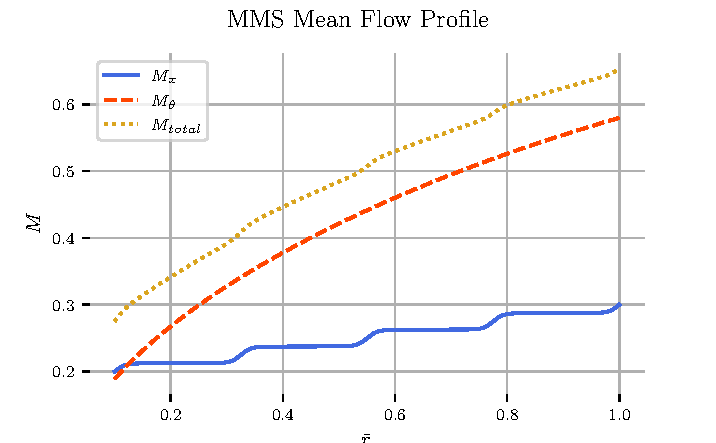
\includegraphics{/home/jeff-severino/SWIRL/CodeRun/04-plotReport/tex-outputs/MMS_mean_flow_profile.pdf}
    \caption{The manufactured mean flow test case using a summation of Tangents for $A$ and $M_x$}
    \label{fig:1}
\end{figure}


\begin{figure}[!]
    \centering
    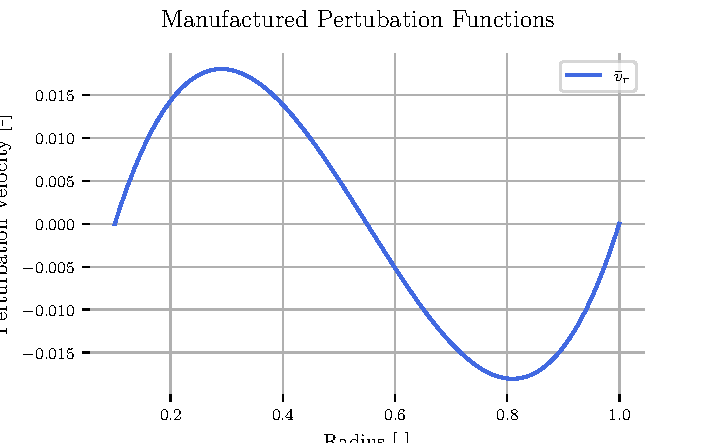
\includegraphics{/home/jeff-severino/SWIRL/CodeRun/04-plotReport/tex-outputs/MMS_perturbation_variables_vR.pdf}
\caption{The manufactured perturbation functions ,$v_r$}%, $v_x$, $v_{\theta}$, $p$}
    \label{fig:1a}
\end{figure}


\begin{figure}[!]
    \centering
    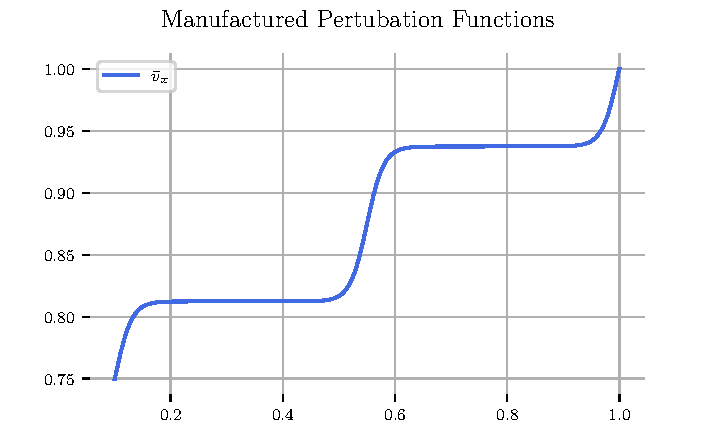
\includegraphics{/home/jeff-severino/SWIRL/CodeRun/04-plotReport/tex-outputs/MMS_perturbation_variables_vX.pdf}
\caption{The manufactured perturbation functions ,$v_x$}%, $v_x$, $v_{\theta}$, $p$}
    \label{fig:2a}
\end{figure}


\begin{figure}[!]
    \centering
    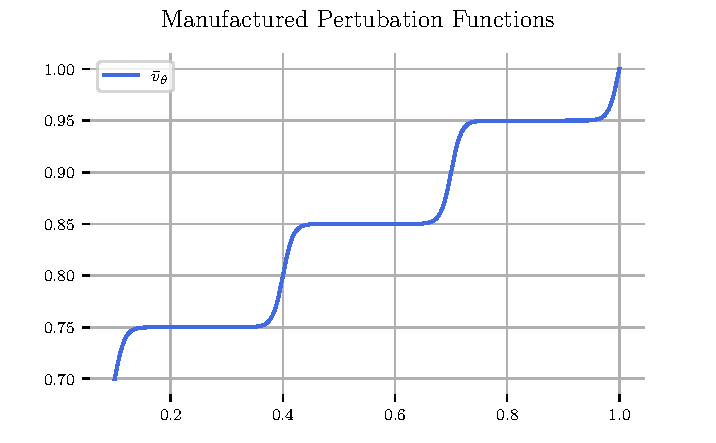
\includegraphics{/home/jeff-severino/SWIRL/CodeRun/04-plotReport/tex-outputs/MMS_perturbation_variables_vTh.pdf}
    \caption{The manufactured perturbation functions ,$v_{\theta}$}%, $v_x$, $v_{\theta}$, $p$}
    \label{fig:3a}
\end{figure}


\begin{figure}[!]
    \centering
    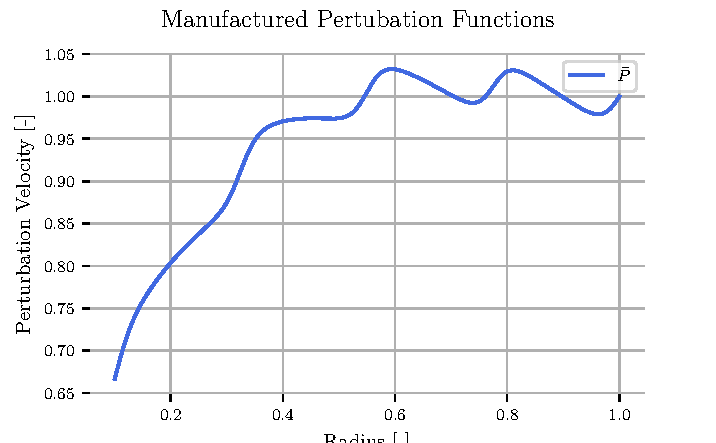
\includegraphics{/home/jeff-severino/SWIRL/CodeRun/04-plotReport/tex-outputs/MMS_perturbation_variables_Pr.pdf}
\caption{The manufactured perturbation functions ,$P$}%, $v_x$, $v_{\theta}$, $p$}
    \label{fig:4a}
\end{figure}

\begin{figure}[!]
    \centering
    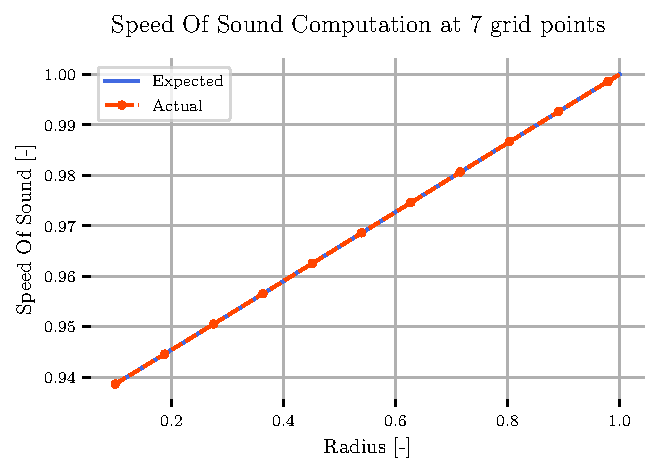
\includegraphics{/home/jeff-severino/SWIRL/CodeRun/04-plotReport/tex-outputs/SpeedOfSoundComparison1.pdf}
    \caption{ A comparison of the speed of sound, expected vs actual at the lowest grid to show similarities in solution}
    \label{fig:5}
\end{figure}


\begin{figure}[!]
    \centering
    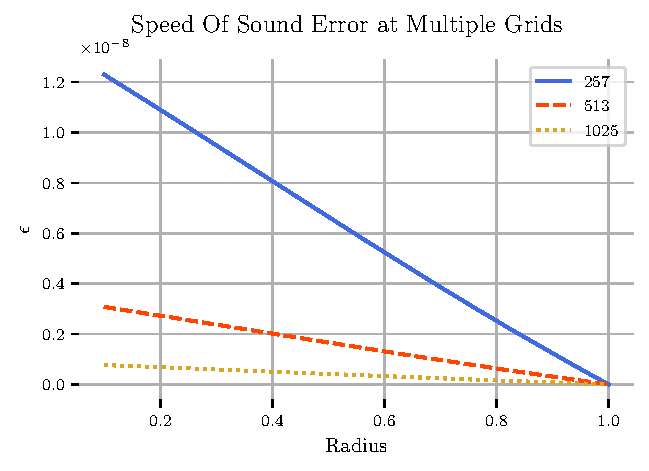
\includegraphics{/home/jeff-severino/SWIRL/CodeRun/04-plotReport/tex-outputs/SpeedOfSoundComparison2.pdf}
    \caption{ A comparison of the speed of sound error at three grid}
    \label{fig:5a}
\end{figure}


\begin{figure}[!]
    \centering
    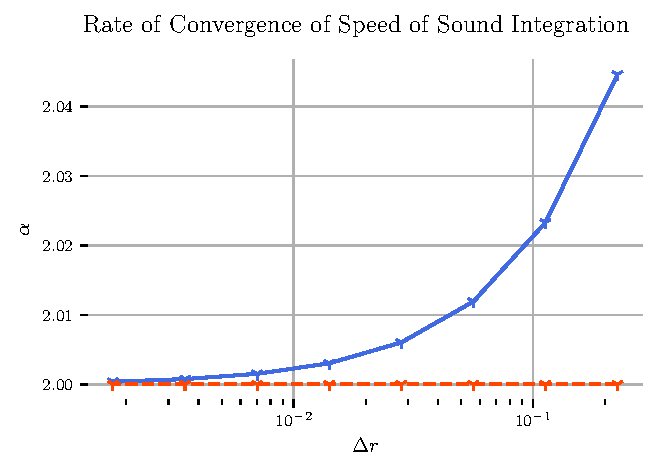
\includegraphics{/home/jeff-severino/SWIRL/CodeRun/04-plotReport/tex-outputs/SND_ROC.pdf}
    \caption{ A comparison of the speed of sound error at three grid}
    \label{fig:5a}
\end{figure}



\begin{figure}[!]
    \centering
    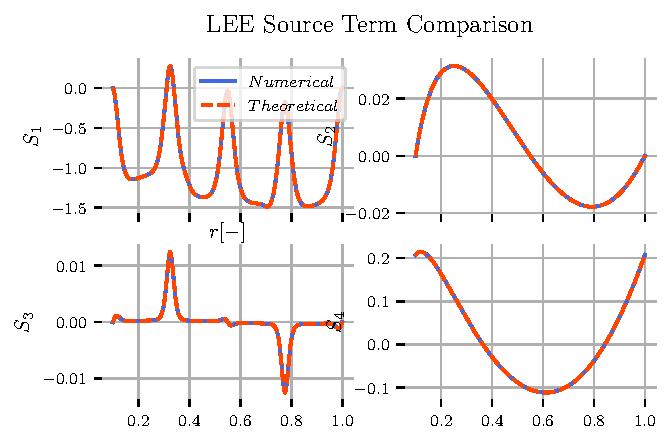
\includegraphics{/home/jeff-severino/SWIRL/CodeRun/04-plotReport/tex-outputs/SourceTermComparison.pdf}
    \caption{LEE Source Terms}
    \label{fig:6}
\end{figure}


\begin{figure}[!]
    \centering
    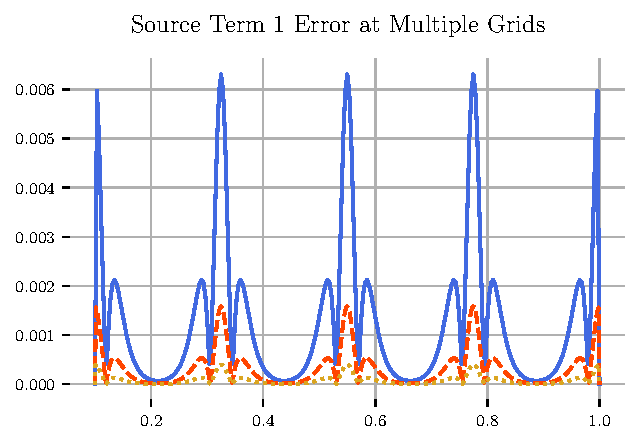
\includegraphics{/home/jeff-severino/SWIRL/CodeRun/04-plotReport/tex-outputs/SourceTermError1.pdf}
    \caption{LEE Source Term Error}
    \label{fig:7}
\end{figure}


\begin{figure}[!]
    \centering
    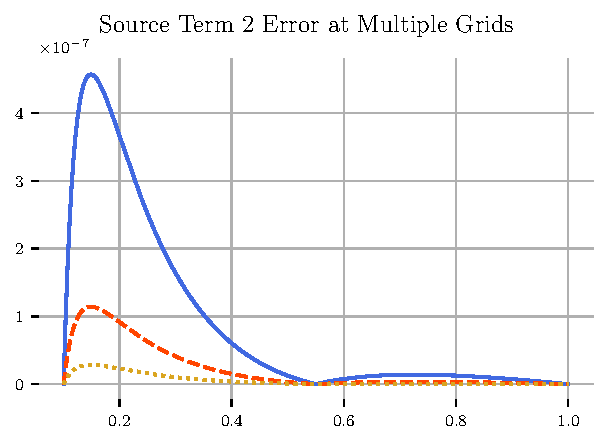
\includegraphics{/home/jeff-severino/SWIRL/CodeRun/04-plotReport/tex-outputs/SourceTermError2.pdf}
    \caption{LEE Source Term Error}
    \label{fig:7}
\end{figure}


\begin{figure}[!]
    \centering
    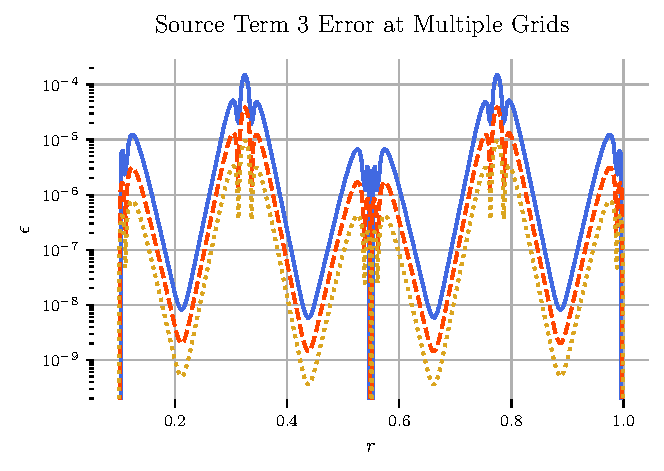
\includegraphics{/home/jeff-severino/SWIRL/CodeRun/04-plotReport/tex-outputs/SourceTermError3.pdf}
    \caption{LEE Source Term Error}
    \label{fig:7}
\end{figure}


\begin{figure}[!]
    \centering
    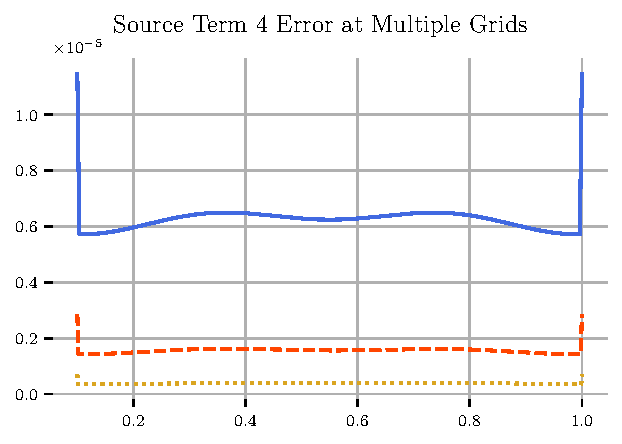
\includegraphics{/home/jeff-severino/SWIRL/CodeRun/04-plotReport/tex-outputs/SourceTermError4.pdf}
    \caption{LEE Source Term Error}
    \label{fig:7}
\end{figure}

\begin{figure}[!]
    \centering
    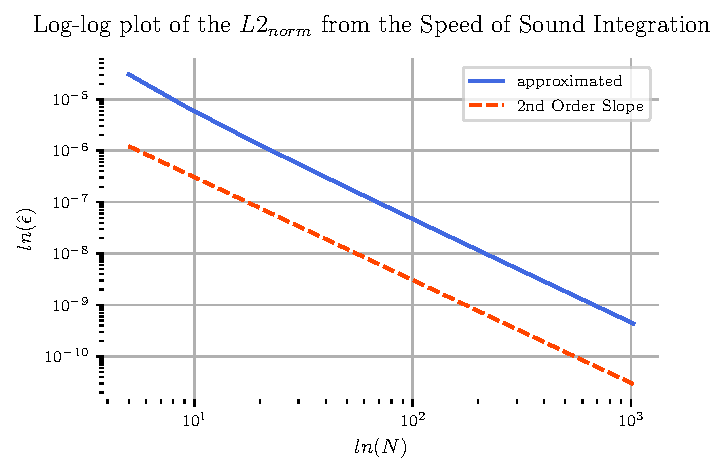
\includegraphics{/home/jeff-severino/SWIRL/CodeRun/04-plotReport/tex-outputs/SND_L2.pdf}
    \caption{L2 Norm comparison for the speed of sound integration for the compound trapezoidal rule}
    \label{fig:8}
\end{figure}



\begin{figure}[!]
    \centering
    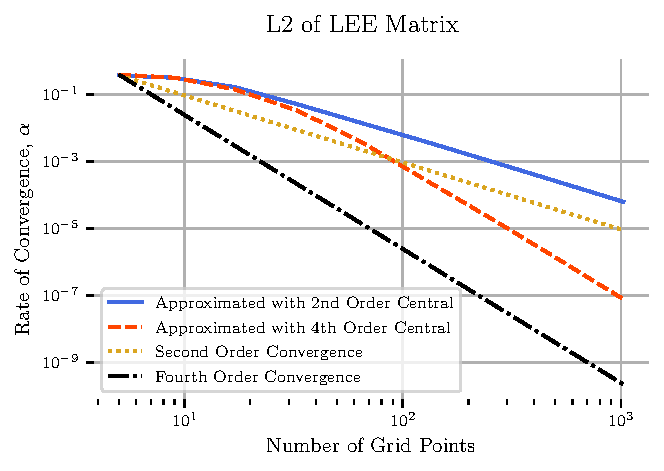
\includegraphics{/home/jeff-severino/SWIRL/CodeRun/04-plotReport/tex-outputs/LEE_L2.pdf}
    \caption{ROC  for the speed of sound integration for the compound trapezoidal rule}
    \label{fig:9}
\end{figure}


\begin{figure}[!]
    \centering
        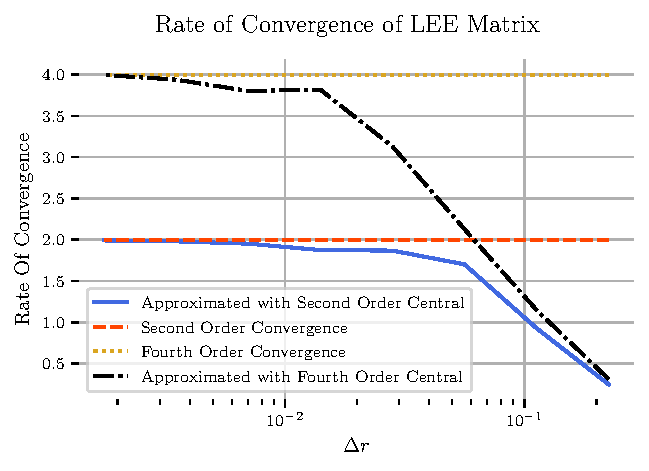
\includegraphics{/home/jeff-severino/SWIRL/CodeRun/04-plotReport/tex-outputs/LEE_ROC.pdf}
       \caption{ROC for the LEE using second and fourth order central differencing
       for the radial derivative}
        \label{fig:10}
\end{figure}





%%\begin{itemize}
%%    \item Kousen's Test Cases
%%        \subitem Cylinder, Uniform Flow with Liner (Table 4.3)
%%        \begin{align*}
%%            m &= 2 \\
%%            k &= \frac{\omega r_T}{A_T} = -1 \\
%%            M_x &= 0.5 \\
%%            \eta_T &= 0.72 + 0.42i\\
%%            \text{Confirm if 32 grid points is enough}
%%        \end{align*} 
%%        \subitem Cylinder, Shear Flow without Liner (Table 4.4)
%%        \begin{align*}
%%            m &= 0 \\
%%            kb &= \left(\frac{\omega r_T}{A_T}\right)b = 20 \\
%%            b &= r_{max} - r_{min} \\
%%            \tilde{r} = \frac{r}{b} \\
%%            M_x &= 0.3(1-\tilde{r})^{\frac{1}{7}} \\
%%            \eta_T &= 0\\
%%            \text{Confirm if 32 grid points is enough}
%%        \end{align*}
%%        \subitem Annulus, Shear Flow without Liner (Table 4.5)
%%        \begin{align*}
%%            m &= 0 \\
%%            kb &= \left(\frac{\omega r_T}{A_T}\right)b = 10 \\
%%            b &= r_{max} - r_{min}  = \frac{1}{7}\\
%%            k &= 70 \\
%%            \tilde{r} = \frac{r}{b} = 6.0 \\
%%            M_x &= 0.3\left(1 - 2 \left| \frac{r_{max}-r}{b} + 0.5 \right|  \right)^{\frac{1}{7}} \\
%%            \eta_T &= 0\\
%%            \text{Confirm if 32 grid points is enough}
%%        \end{align*}
%%        \subitem Annulus, Shear Flow with Liner (Table 4.6)
%%        \begin{align*}
%%            m &= 0 \\
%%            kb &= \left(\frac{\omega r_T}{A_T}\right)b = 10 \\
%%            b &= r_{max} - r_{min}  = \frac{1}{3}\\
%%            k &= 30 \\
%%            \tilde{r} = \frac{r}{b} = 2.0 \\
%%            M_x &= 0.3\left(1 - 2 \left| \frac{r_{max}-r}{b} + 0.5 \right|  \right)^{\frac{1}{7}} \\
%%            \eta_T &= 0.3 + 0.1i\\
%%            \text{Confirm if 32 grid points is enough}
%%        \end{align*}
%%\end{itemize}
\subsubsection{Test Case 1}
A comparison was conducted for a hollow cylinder undergoing uniform flow with
acoustic liners along the outer duct perimeter. The azimuthal mode number, reduced 
frequency, mach number and duct liner admittance is reported below,
\begin{align*}
    m &= 2 \\
    k &= \frac{\omega r_T}{A_T} = -1 \\
    M_x &= 0.5 \\
    \eta_T &= 0.72 + 0.42i
\end{align*} 
\begin{figure}[h!]
    \centering
    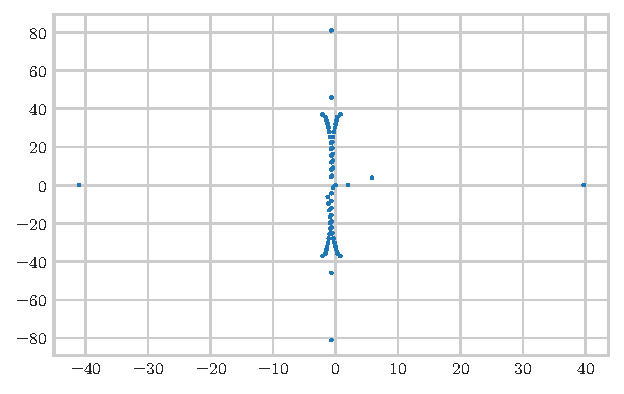
\includegraphics[width=\textwidth]{Chapter-5-Results/tex-outputs/gam.acc.scatter.Table4.3.pdf}
\end{figure}

\begin{figure}[h!]
    \centering
    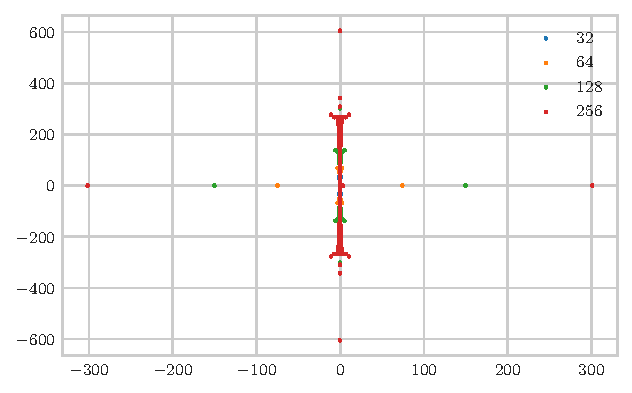
\includegraphics[width=\textwidth]{/home/jeff-severino/SWIRL/CodeRun/04-plotReport/tex-outputs/gam.nonconv.scatter_2nd_ord_comp.pdf}
\end{figure}

\begin{figure}[h!]
    \centering
    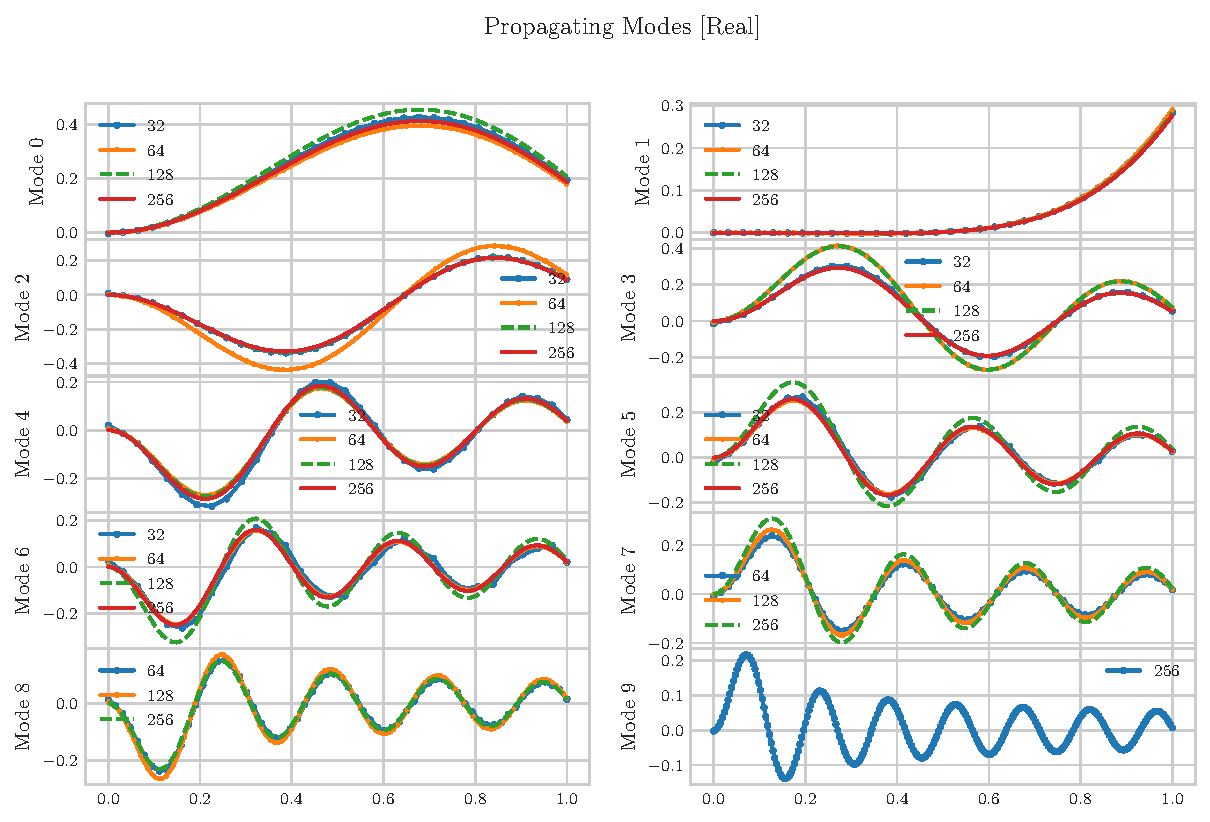
\includegraphics[width=\textwidth]{/home/jeff-severino/SWIRL/CodeRun/04-plotReport/tex-outputs/egv_prop_re.pdf}
    \label{fig:prop_re}
\end{figure}

\begin{figure}[h!]
    \centering
    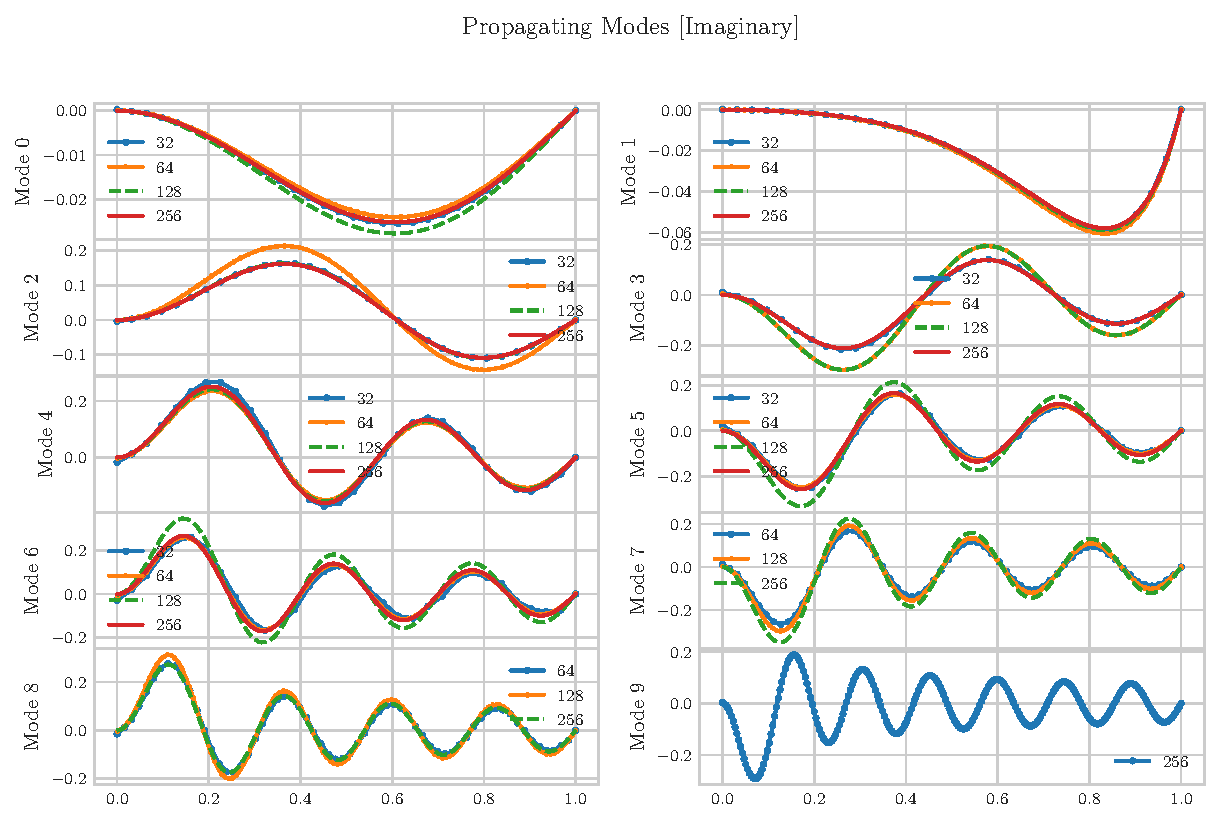
\includegraphics[width=\textwidth]{/home/jeff-severino/SWIRL/CodeRun/04-plotReport/tex-outputs/egv_prop_im.pdf}
    \label{fig:prop_im}
\end{figure}

\begin{figure}[h!]
    \centering
    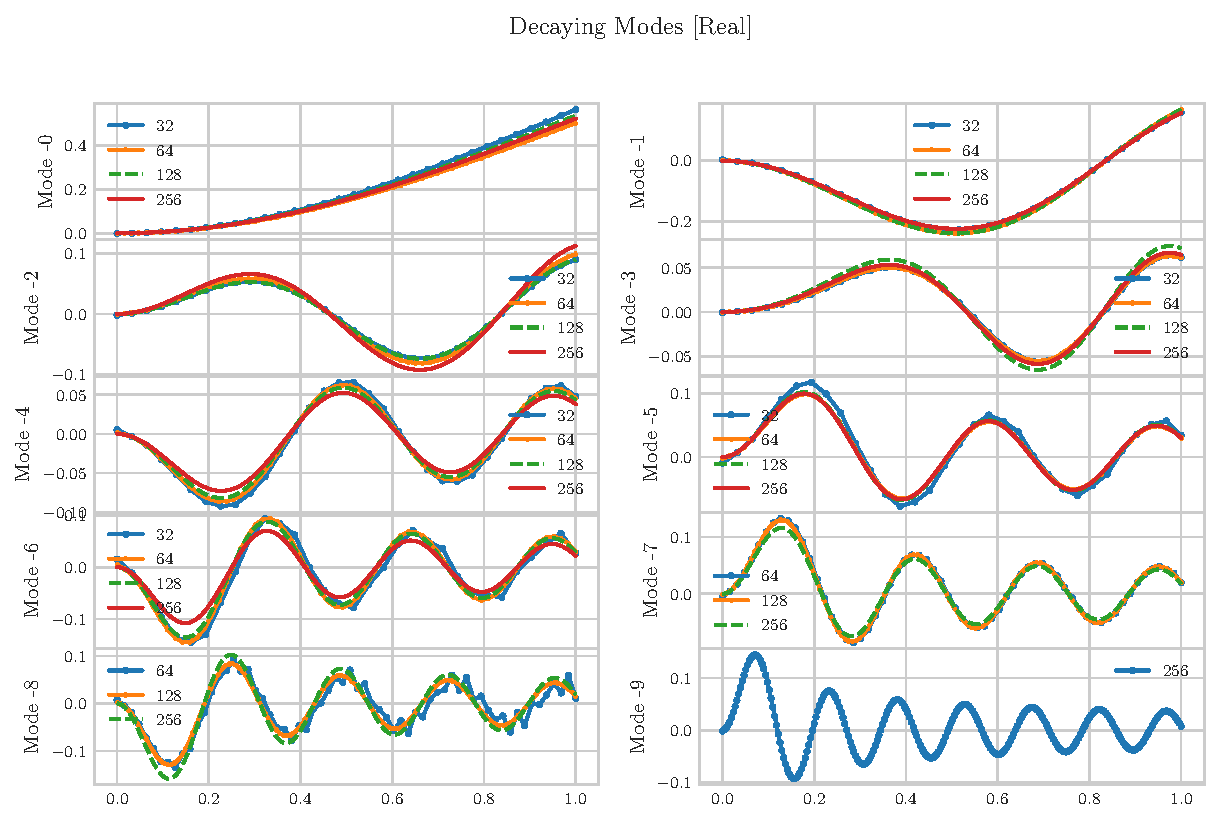
\includegraphics[width=\textwidth]{/home/jeff-severino/SWIRL/CodeRun/04-plotReport/tex-outputs/egv_decay_re.pdf}
    \label{fig:decay_re} 
\end{figure}

\begin{figure}[h!]
    \centering
    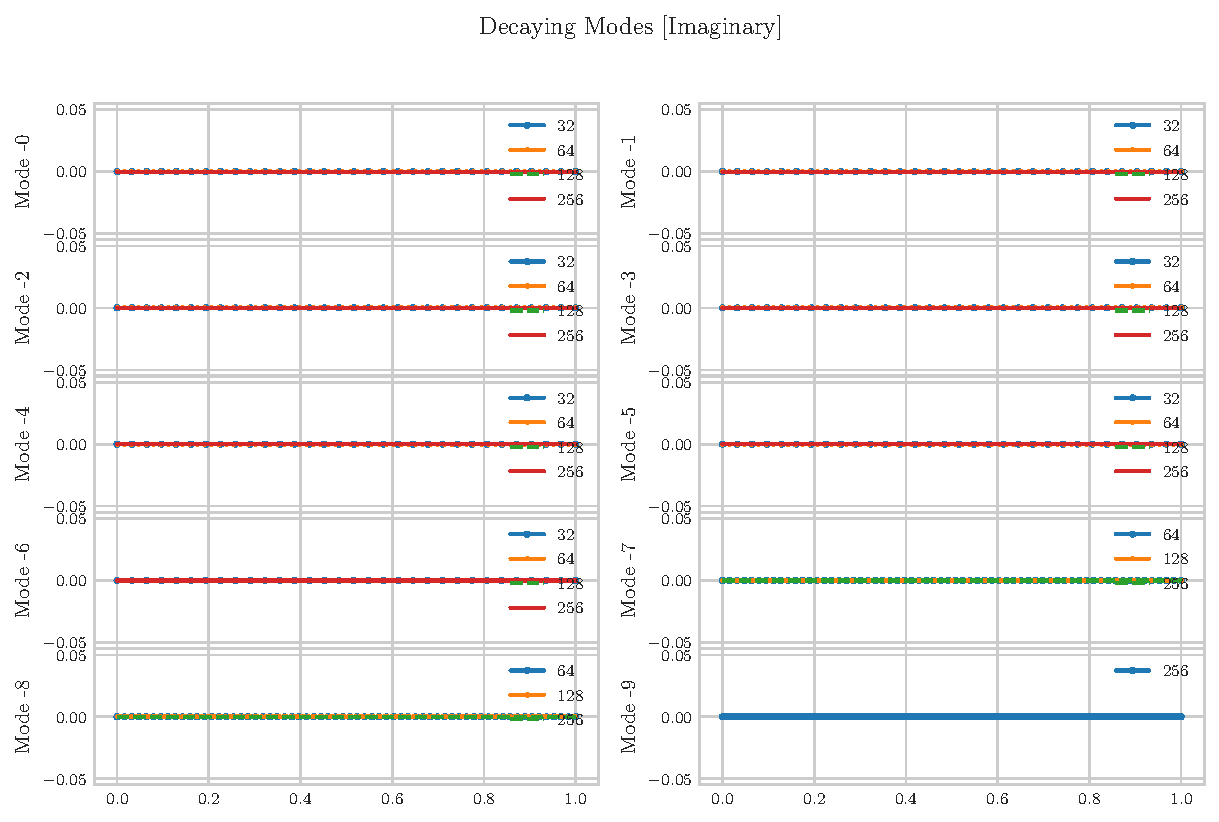
\includegraphics[width=\textwidth]{/home/jeff-severino/SWIRL/CodeRun/04-plotReport/tex-outputs/egv_decay_im.pdf}
    \label{fig:decay_im} 
\end{figure}








The results shown in \ref{Table43} are in moderately good agreement. The 
results were obtained by visually comparing the output in \verb|gam.acc| for 32 
grid points. Note that the indicies for the SWIRL deliverable are different that 
the ones obtained for the most recent version of the code. While the 
convective axial wavenumbers show agreement to machine precision, this is not 
particularly insightful given that there are an infinite number of possible solutions 
that could satisfy the eigenvalue problem. The results that are of concern 
are propagating modes that are not convecting with the mean flow.  The scatter plot
of the axial wavenumbers show some sporadic behaviour around the imaginary axis.
The results from the MMS along with this plot indicate that more grid points are going 
to be needed if a finite difference technique is to be used.

The first 10 propagating and decaying modes are plotted in \ref{fig:prop_re}-\ref{fig:decay_im}.



% It should be 
% noted that a spectral differencing method were using for Kousen's report and for
% srcF2008. 
%Using a higher order scheme would also improve accuracy.


\begin{table}
 \centering
 \begin{adjustbox}{width=1\textwidth}
     \small
 \begin{tabular}{c | r | r | r | r | r | r}
 \hline
 $\gamma^{\pm}_n$ & Kousen Ref. [15] & Kousen report & srcF2008 & index  & current & index\\
 \hline
 $\gamma_0^{+}$ & $ 0.620 - 5.014  i $ & $ 0.6195 - 5.0139 i$ & $ 0.61954  - 5.01386 i$ & 60  & 0.620755853112 - 5.00592416941i& 34 \\
 $\gamma_1^{+}$ & $-5.820 - 3.897  i $ & $-5.8195 - 3.8968 i$ & $-5.81953  - 3.89677 i$ & 58  &-0.581267772517 - 3.90050864568i& 33 \\
 $\gamma_2^{+}$ & $ 0.445 - 9.187  i $ & $ 0.4453 - 9.1868 i$ & $ 0.44533  - 9.18684 i$ & 59  &0.451569491142 -  9.12191317214i & 31 \\
 $\gamma_3^{+}$ & $ 0.453 - 13.062 i $ & $ 0.4539 - 13.062 i$ & $ 0.45389  - 13.0615 i$ & 57  &0.464247902898 - 12.8487472519i & 29 \\ 
 $\gamma_4^{+}$ & $ 0.480 - 16.822 i $ & $ 0.4795 - 16.822 i$ & $ 0.47952  - 16.8216 i$ & 55  &0.492340380223 - 16.3292825150i & 27 \\
 $\gamma_5^{+}$ & $ 0.503 - 20.531 i $ & $ 0.5029 - 20.531 i$ & $ 0.50287  - 20.5307 i$ & 51  &0.514522630594 -19.5817182568i& 25 \\
 $\gamma_6^{+}$ & $ 0.522 - 24.213 i $ & $ 0.5220 - 24.213 i$ & $ 0.52202  - 24.2129 i$ & 50  &0.516658239854 -22.5715880605i& 23 \\
 $\gamma_7^{+}$ & $ 0.538 - 27.880 i $ & $ 0.5376 - 27.880 i$ & $ 0.53754  - 27.8800 i$ & 48  & - & - \\
 $\gamma_8^{+}$ & $ 0.550 - 31.537 i $ & $ 0.5502 - 31.537 i$ & $ 0.55024  - 31.5368 i$ & 47  & - & - \\
 $\gamma_9^{+}$ & $ 0.589 - 49.75  i $ & $ 0.5891 - 49.754 i$ & $ 0.58745  - 49.7669 i$ & 33  &- &- \\ \hline
 $\gamma_0^{-}$ & $ 0.410 + 1.290  i $ & $ 0.4101 + 1.2904 i$ & $ 0.41009  + 1.29037 i$ & 64  &0.409973310292  + 1.29020083859i& 64 \\
 $\gamma_1^{-}$ & $ 1.259 + 6.085  i $ & $ 1.2595 + 6.0852 i$ & $ 1.25949  + 6.08517 i$ & 63  &1.25530612217  + 6.07214375548i & 62 \\
 $\gamma_2^{-}$ & $ 1.146 + 9.668  i $ & $ 1.1457 + 9.6679 i$ & $ 1.14567  + 9.66787 i$ & 62  &1.13696444935  + 9.59622801724i &  60\\
$\gamma_3^{-}$ & $ 1.022 + 13.315 i $ & $ 1.0218 + 13.315 i$ & $ 1.02183  + 13.3150 i$ & 61  &1.00950576515 + 13.0957277529i & 58  \\
 $\gamma_4^{-}$ & $ 0.943 + 16.977 i $ & $ 0.9425 + 16.977 i$ & $ 0.94250  + 16.9767 i$ & 56  &0.928059983039 +  16.4791343118i& 56  \\
 $\gamma_5^{-}$ & $ 0.891 + 20.635 i $ & $ 0.8908 + 20.635 i$ & $ 0.89075  + 20.6353 i$ & 54  &0.856678172769 +  22.6544943903i & 52 \\
 $\gamma_6^{-}$ & $ 0.855 + 24.288 i $ & $ 0.8549 + 24.288 i$ & $ 0.85490  + 24.2883 i$ & 53  &0.941762848775 +  25.3460188358i & 50 \\
 $\gamma_7^{-}$ & $ 0.829 + 27.937 i $ & $ 0.8288 + 27.937 i$ & $ 0.82877  + 27.9369 i$ & 52  &- & - \\
 $\gamma_8^{-}$ & $ 0.809 + 31.581 i $ & $ 0.8089 + 31.581 i$ & $ 0.80891  + 31.5812 i$ & 49  &- & - \\
 $\gamma_9^{-}$ & $ 0.755 + 49.77  i $ & $ 0.7547 + 49.772 i$ & $ 0.75658  + 49.7851 i$ & 39  &- & - \\ \hline
 \end{tabular}
\end{adjustbox}
 \caption{Table 4.3 data}
 \label{Table43}
\end{table}


    -
%\subsection{Method of Manufactured Solution Results}

%\begin{figure}
%    \centering
%    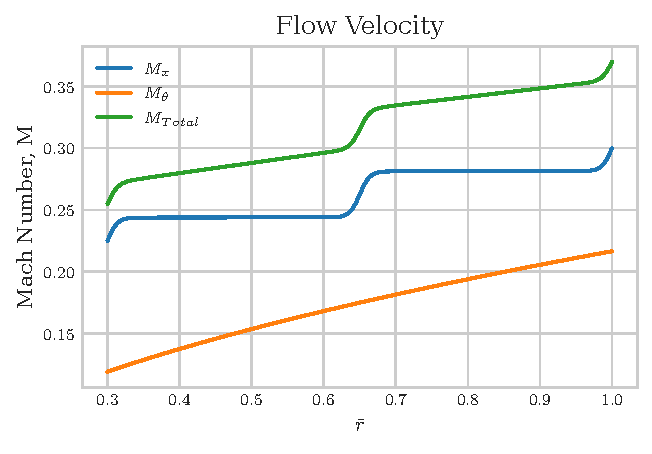
\includegraphics[width=\textwidth]{Chapter-5-Results/tex-outputs/MachDistribution_R1.pdf}
%    \caption{Mach distribution for method of manufactured solution case}
%\end{figure}

% \begin{figure}
%     \centering
%     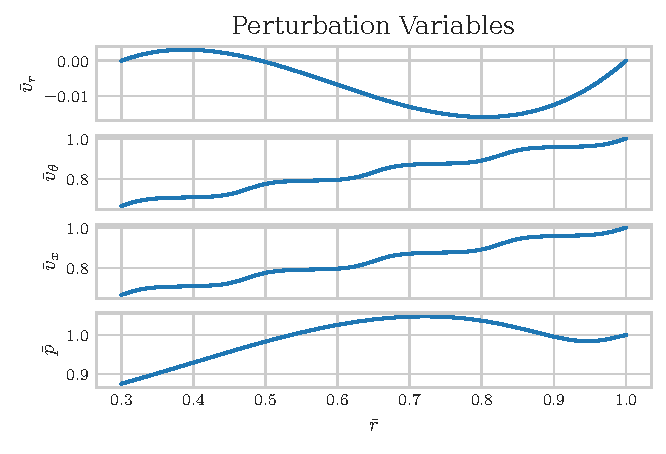
\includegraphics[width=\textwidth]{Chapter-5-Results/tex-outputs/PerturbationVariables_R1.pdf}
% \end{figure}

% \begin{figure}
%     \centering
%         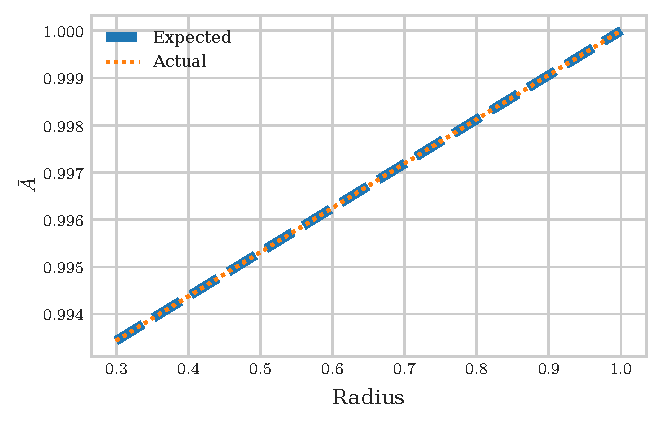
\includegraphics[width=\textwidth]{Chapter-5-Results/tex-outputs/SoundSpeedFromIntegration_R1.pdf}
%     \caption{Speed of Sound from Integrating the Tangential Mach Number}
% \end{figure}

% \begin{figure}
%     \centering
%         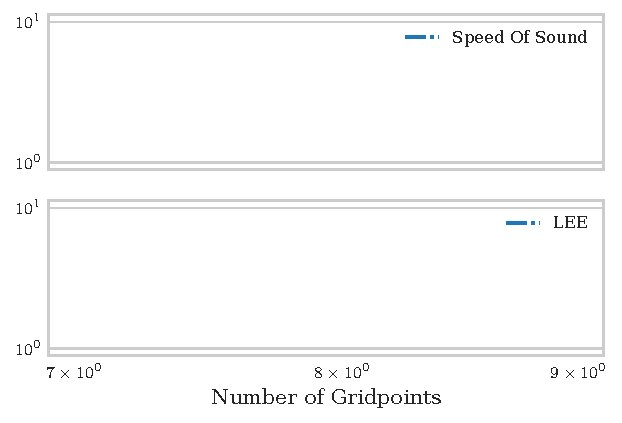
\includegraphics[width=\textwidth]{Chapter-5-Results/tex-outputs/L2_R1.pdf}
%     \caption{L2 Norm of the Error for the MMS as a function of Grid Points}
% \end{figure}

% \begin{figure}
%     \centering
%         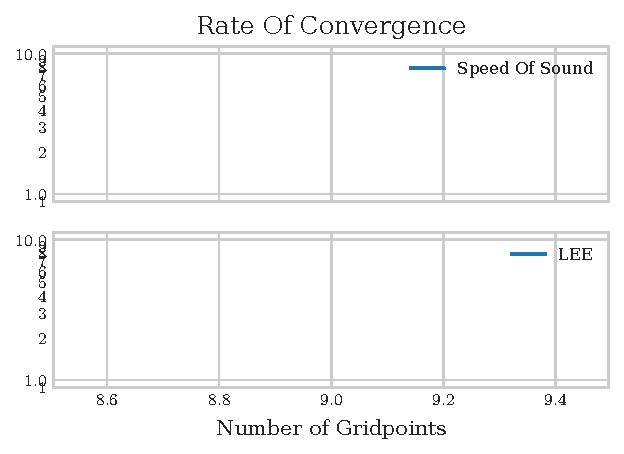
\includegraphics[width=\textwidth]{Chapter-5-Results/tex-outputs/ROC_R1.pdf}
%     \caption{Rate of Convergence for the Speed of Sound Integration}
% \end{figure}

% \begin{figure}
%     \centering
%         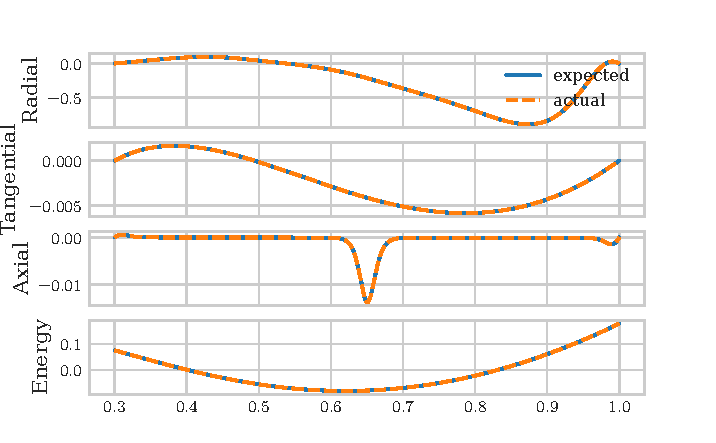
\includegraphics[width=\textwidth]{Chapter-5-Results/tex-outputs/SourceTermData_R1.pdf}
%     \caption{Source Term Error}
% \end{figure}
%%
%%%the thesis class is messing up figures. Cant put in figure statement
%%    % This file was created with tikzplotlib v0.9.12.
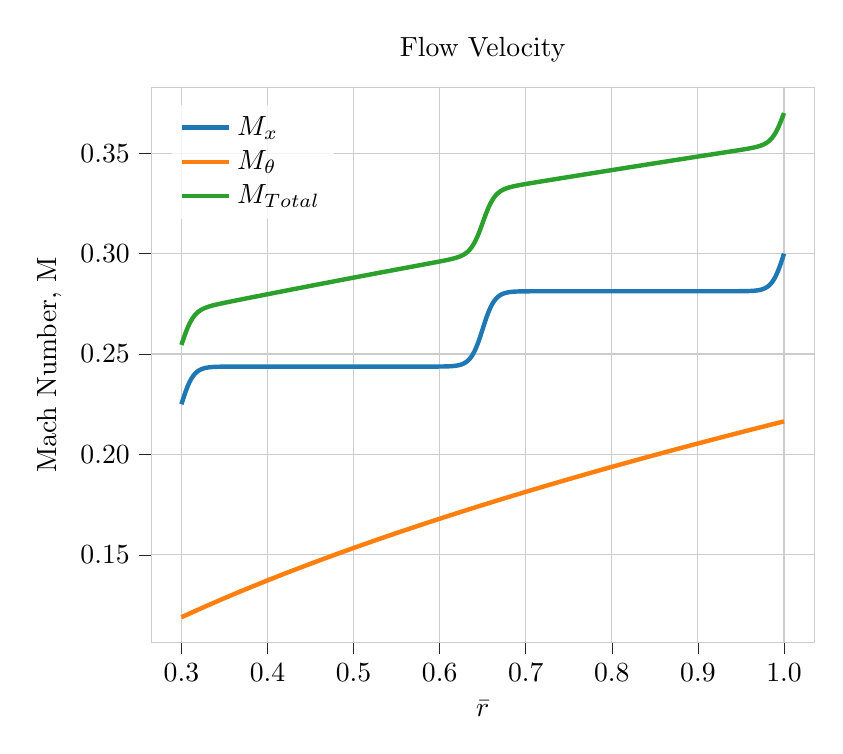
\begin{tikzpicture}

\definecolor{color0}{rgb}{0.12156862745098,0.466666666666667,0.705882352941177}
\definecolor{color1}{rgb}{1,0.498039215686275,0.0549019607843137}
\definecolor{color2}{rgb}{0.172549019607843,0.627450980392157,0.172549019607843}

\begin{axis}[
axis line style={white!80!black},
legend cell align={left},
legend style={
  fill opacity=0.8,
  draw opacity=1,
  text opacity=1,
  at={(0.03,0.97)},
  anchor=north west,
  draw=none
},
tick align=outside,
tick pos=left,
title={Flow Velocity},
width=10cm,
x grid style={white!80!black},
xlabel={\(\displaystyle \bar{r}\)},
xmajorgrids,
xmin=0.265, xmax=1.035,
xtick style={color=white!15!black},
xtick={0.2,0.3,0.4,0.5,0.6,0.7,0.8,0.9,1,1.1},
xticklabels={0.2,0.3,0.4,0.5,0.6,0.7,0.8,0.9,1.0,1.1},
y grid style={white!80!black},
ylabel={Mach Number, M},
ymajorgrids,
ymin=0.106407621216694, ymax=0.382495062973916,
ytick style={color=white!15!black},
ytick={0.1,0.15,0.2,0.25,0.3,0.35,0.4},
yticklabels={0.10,0.15,0.20,0.25,0.30,0.35,0.40}
]
\addplot [ultra thick, color0]
table {%
0.3 0.225
0.30068093385214 0.225911246524957
0.30136186770428 0.226818198570373
0.30204280155642 0.227716642232255
0.30272373540856 0.228602521566251
0.3034046692607 0.229472009803963
0.30408560311284 0.230321571833456
0.304766536964981 0.231148015936729
0.305447470817121 0.231948533436318
0.306128404669261 0.232720725601336
0.306809338521401 0.233462617841939
0.307490272373541 0.234172661829725
0.308171206225681 0.234849726682304
0.308852140077821 0.235493080720102
0.309533073929961 0.236102365534612
0.310214007782101 0.236677564205243
0.310894941634241 0.237218965482389
0.311575875486381 0.237727125639891
0.312256809338521 0.238202829516209
0.312937743190661 0.238647052036056
0.313618677042802 0.239060921256205
0.314299610894942 0.239445683730185
0.314980544747082 0.239802672751423
0.315661478599222 0.240133279823468
0.316342412451362 0.240438929525229
0.317023346303502 0.240721057791178
0.317704280155642 0.240981093510991
0.318385214007782 0.241220443267894
0.319066147859922 0.241440478976642
0.319747081712062 0.241642528146511
0.320428015564202 0.24182786647775
0.321108949416342 0.241997712497462
0.321789883268483 0.242153223949324
0.322470817120623 0.242295495667554
0.323151750972763 0.242425558686559
0.323832684824903 0.242544380361487
0.324513618677043 0.242652865299888
0.325194552529183 0.242751856929575
0.325875486381323 0.242842139551689
0.326556420233463 0.242924440750359
0.327237354085603 0.242999434050808
0.327918287937743 0.243067741736172
0.328599221789883 0.243129937749575
0.329280155642023 0.24318655062221
0.329961089494163 0.243238066380449
0.330642023346304 0.243284931395434
0.331322957198444 0.243327555147452
0.332003891050584 0.243366312884698
0.332684824902724 0.243401548162173
0.333365758754864 0.243433575251368
0.334046692607004 0.243462681415434
0.334727626459144 0.243489129047703
0.335408560311284 0.243513157673944
0.336089494163424 0.243534985820668
0.336770428015564 0.243554812753243
0.337451361867704 0.243572820088649
0.338132295719844 0.243589173288439
0.338813229571985 0.243604023037975
0.339494163424124 0.243617506518261
0.340175097276265 0.243629748576837
0.340856031128405 0.243640862804179
0.341536964980545 0.243650952521944
0.342217898832685 0.24366011168923
0.342898832684825 0.243668425732785
0.343579766536965 0.243675972306829
0.344260700389105 0.243682821987882
0.344941634241245 0.243689038909678
0.345622568093385 0.24369468134292
0.346303501945525 0.243699802224365
0.346984435797665 0.243704449639386
0.347665369649805 0.243708667261887
0.348346303501946 0.243712494755159
0.349027237354086 0.243715968136995
0.349708171206226 0.243719120112134
0.350389105058366 0.243721980374849
0.351070038910506 0.243724575884284
0.351750972762646 0.243726931114917
0.352431906614786 0.24372906828436
0.353112840466926 0.243731007560471
0.353793774319066 0.243732767249647
0.354474708171206 0.243734363967963
0.355155642023346 0.243735812796689
0.355836575875487 0.243737127423603
0.356517509727627 0.243738320271376
0.357198443579767 0.243739402614186
0.357879377431907 0.243740384683649
0.358560311284047 0.243741275765012
0.359241245136187 0.243742084284522
0.359922178988327 0.243742817888744
0.360603112840467 0.243743483516595
0.361284046692607 0.243744087464733
0.361964980544747 0.243744635446923
0.362645914396887 0.243745132647937
0.363326848249027 0.243745583772469
0.364007782101167 0.243745993089547
0.364688715953307 0.243746364472841
0.365369649805448 0.243746701437242
0.366050583657588 0.243747007172075
0.366731517509728 0.243747284571228
0.367412451361868 0.243747536260505
0.368093385214008 0.243747764622448
0.368774319066148 0.243747971818859
0.369455252918288 0.243748159811245
0.370136186770428 0.243748330379367
0.370817120622568 0.243748485138073
0.371498054474708 0.243748625552576
0.372178988326848 0.243748752952309
0.372859922178988 0.243748868543514
0.373540856031128 0.243748973420646
0.374221789883268 0.243749068576732
0.374902723735409 0.243749154912772
0.375583657587549 0.243749233246265
0.376264591439689 0.243749304318942
0.376945525291829 0.243749368803793
0.377626459143969 0.243749427311433
0.378307392996109 0.243749480395884
0.378988326848249 0.243749528559818
0.379669260700389 0.243749572259319
0.380350194552529 0.243749611908196
0.381031128404669 0.243749647881906
0.381712062256809 0.243749680521103
0.38239299610895 0.24374971013487
0.38307392996109 0.243749737003639
0.38375486381323 0.243749761381848
0.38443579766537 0.243749783500355
0.38511673151751 0.243749803568616
0.38579766536965 0.243749821776675
0.38647859922179 0.243749838296959
0.38715953307393 0.243749853285912
0.38784046692607 0.24374986688548
0.38852140077821 0.243749879224449
0.38920233463035 0.243749890419668
0.38988326848249 0.243749900577155
0.39056420233463 0.243749909793102
0.39124513618677 0.243749918154784
0.391926070038911 0.243749925741385
0.392607003891051 0.243749932624752
0.393287937743191 0.243749938870069
0.393968871595331 0.24374994453648
0.394649805447471 0.243749949677647
0.395330739299611 0.243749954342256
0.396011673151751 0.243749958574482
0.396692607003891 0.243749962414403
0.397373540856031 0.243749965898385
0.398054474708171 0.243749969059421
0.398735408560311 0.243749971927446
0.399416342412451 0.243749974529621
0.400097276264592 0.243749976890588
0.400778210116732 0.243749979032707
0.401459143968872 0.243749980976262
0.402140077821012 0.243749982739661
0.402821011673152 0.243749984339602
0.403501945525292 0.243749985791237
0.404182879377432 0.243749987108313
0.404863813229572 0.243749988303304
0.405544747081712 0.243749989387525
0.406225680933852 0.243749990371245
0.406906614785992 0.243749991263779
0.407587548638132 0.24374999207358
0.408268482490272 0.243749992808317
0.408949416342412 0.243749993474948
0.409630350194553 0.243749994079785
0.410311284046693 0.243749994628558
0.410992217898833 0.243749995126462
0.411673151750973 0.243749995578213
0.412354085603113 0.243749995988089
0.413035019455253 0.243749996359972
0.413715953307393 0.243749996697383
0.414396887159533 0.243749997003518
0.415077821011673 0.243749997281276
0.415758754863813 0.243749997533287
0.416439688715953 0.243749997761938
0.417120622568093 0.243749997969395
0.417801556420233 0.243749998157621
0.418482490272374 0.2437499983284
0.419163424124514 0.243749998483348
0.419844357976654 0.243749998623934
0.420525291828794 0.243749998751488
0.421206225680934 0.243749998867218
0.421887159533074 0.243749998972221
0.422568093385214 0.243749999067491
0.423249027237354 0.24374999915393
0.423929961089494 0.243749999232356
0.424610894941634 0.243749999303512
0.425291828793774 0.243749999368073
0.425972762645914 0.24374999942665
0.426653696498055 0.243749999479796
0.427334630350195 0.243749999528016
0.428015564202335 0.243749999571767
0.428696498054475 0.243749999611462
0.429377431906615 0.243749999647478
0.430058365758755 0.243749999680155
0.430739299610895 0.243749999709803
0.431420233463035 0.243749999736703
0.432101167315175 0.243749999761109
0.432782101167315 0.243749999783253
0.433463035019455 0.243749999803345
0.434143968871595 0.243749999821574
0.434824902723735 0.243749999838113
0.435505836575875 0.24374999985312
0.436186770428016 0.243749999866735
0.436867704280156 0.243749999879088
0.437548638132296 0.243749999890297
0.438229571984436 0.243749999900466
0.438910505836576 0.243749999909693
0.439591439688716 0.243749999918065
0.440272373540856 0.24374999992566
0.440953307392996 0.243749999932552
0.441634241245136 0.243749999938805
0.442315175097276 0.243749999944478
0.442996108949416 0.243749999949626
0.443677042801557 0.243749999954296
0.444357976653696 0.243749999958534
0.445038910505837 0.243749999962379
0.445719844357977 0.243749999965867
0.446400778210117 0.243749999969033
0.447081712062257 0.243749999971905
0.447762645914397 0.243749999974511
0.448443579766537 0.243749999976876
0.449124513618677 0.243749999979022
0.449805447470817 0.243749999980969
0.450486381322957 0.243749999982736
0.451167315175097 0.243749999984339
0.451848249027237 0.243749999985794
0.452529182879377 0.243749999987115
0.453210116731518 0.243749999988313
0.453891050583658 0.243749999989401
0.454571984435798 0.243749999990388
0.455252918287938 0.243749999991285
0.455933852140078 0.243749999992099
0.456614785992218 0.243749999992838
0.457295719844358 0.243749999993509
0.457976653696498 0.243749999994119
0.458657587548638 0.243749999994673
0.459338521400778 0.243749999995176
0.460019455252918 0.243749999995634
0.460700389105058 0.243749999996051
0.461381322957198 0.24374999999643
0.462062256809338 0.243749999996776
0.462743190661479 0.24374999999709
0.463424124513619 0.243749999997378
0.464105058365759 0.24374999999764
0.464785992217899 0.24374999999788
0.465466926070039 0.243749999998101
0.466147859922179 0.243749999998302
0.466828793774319 0.243749999998489
0.467509727626459 0.24374999999866
0.468190661478599 0.243749999998819
0.468871595330739 0.243749999998967
0.469552529182879 0.243749999999105
0.47023346303502 0.243749999999235
0.47091439688716 0.243749999999357
0.4715953307393 0.243749999999473
0.47227626459144 0.243749999999584
0.47295719844358 0.243749999999692
0.47363813229572 0.243749999999796
0.47431906614786 0.243749999999898
0.475 0.24375
0.47568093385214 0.243750000000101
0.47636186770428 0.243750000000204
0.47704280155642 0.243750000000308
0.47772373540856 0.243750000000416
0.4784046692607 0.243750000000527
0.47908560311284 0.243750000000643
0.479766536964981 0.243750000000765
0.480447470817121 0.243750000000895
0.481128404669261 0.243750000001033
0.481809338521401 0.243750000001181
0.482490272373541 0.24375000000134
0.483171206225681 0.243750000001511
0.483852140077821 0.243750000001697
0.484533073929961 0.2437500000019
0.485214007782101 0.243750000002119
0.485894941634241 0.24375000000236
0.486575875486381 0.243750000002622
0.487256809338522 0.24375000000291
0.487937743190662 0.243750000003224
0.488618677042802 0.24375000000357
0.489299610894942 0.243750000003949
0.489980544747082 0.243750000004366
0.490661478599222 0.243750000004823
0.491342412451362 0.243750000005327
0.492023346303502 0.243750000005881
0.492704280155642 0.243750000006491
0.493385214007782 0.243750000007162
0.494066147859922 0.243750000007901
0.494747081712062 0.243750000008715
0.495428015564202 0.243750000009612
0.496108949416342 0.243750000010599
0.496789883268483 0.243750000011687
0.497470817120623 0.243750000012885
0.498151750972763 0.243750000014206
0.498832684824903 0.243750000015661
0.499513618677043 0.243750000017264
0.500194552529183 0.243750000019031
0.500875486381323 0.243750000020978
0.501556420233463 0.243750000023124
0.502237354085603 0.243750000025489
0.502918287937743 0.243750000028095
0.503599221789883 0.243750000030967
0.504280155642023 0.243750000034133
0.504961089494164 0.243750000037621
0.505642023346303 0.243750000041466
0.506322957198444 0.243750000045704
0.507003891050584 0.243750000050374
0.507684824902724 0.243750000055522
0.508365758754864 0.243750000061195
0.509046692607004 0.243750000067448
0.509727626459144 0.24375000007434
0.510408560311284 0.243750000081936
0.511089494163424 0.243750000090307
0.511770428015564 0.243750000099534
0.512451361867704 0.243750000109703
0.513132295719844 0.243750000120911
0.513813229571984 0.243750000133265
0.514494163424124 0.24375000014688
0.515175097276265 0.243750000161887
0.515856031128405 0.243750000178426
0.516536964980545 0.243750000196655
0.517217898832685 0.243750000216747
0.517898832684825 0.243750000238891
0.518579766536965 0.243750000263297
0.519260700389105 0.243750000290197
0.519941634241245 0.243750000319845
0.520622568093385 0.243750000352522
0.521303501945525 0.243750000388538
0.521984435797665 0.243750000428233
0.522665369649805 0.243750000471984
0.523346303501946 0.243750000520204
0.524027237354086 0.24375000057335
0.524708171206226 0.243750000631927
0.525389105058366 0.243750000696487
0.526070038910506 0.243750000767644
0.526750972762646 0.24375000084607
0.527431906614786 0.243750000932509
0.528112840466926 0.243750001027779
0.528793774319066 0.243750001132782
0.529474708171206 0.243750001248512
0.530155642023346 0.243750001376066
0.530836575875486 0.243750001516652
0.531517509727626 0.2437500016716
0.532198443579767 0.243750001842379
0.532879377431907 0.243750002030605
0.533560311284047 0.243750002238062
0.534241245136187 0.243750002466713
0.534922178988327 0.243750002718724
0.535603112840467 0.243750002996482
0.536284046692607 0.243750003302617
0.536964980544747 0.243750003640028
0.537645914396887 0.243750004011911
0.538326848249027 0.243750004421787
0.539007782101167 0.243750004873538
0.539688715953307 0.243750005371442
0.540369649805448 0.243750005920215
0.541050583657588 0.243750006525052
0.541731517509728 0.243750007191683
0.542412451361868 0.24375000792642
0.543093385214008 0.243750008736221
0.543774319066148 0.243750009628755
0.544455252918288 0.243750010612475
0.545136186770428 0.243750011696696
0.545817120622568 0.243750012891687
0.546498054474708 0.243750014208763
0.547178988326848 0.243750015660398
0.547859922178988 0.243750017260339
0.548540856031128 0.243750019023738
0.549221789883269 0.243750020967294
0.549902723735409 0.243750023109412
0.550583657587549 0.243750025470379
0.551264591439689 0.243750028072554
0.551945525291829 0.243750030940579
0.552626459143969 0.243750034101615
0.553307392996109 0.243750037585597
0.553988326848249 0.243750041425518
0.554669260700389 0.243750045657744
0.555350194552529 0.243750050322353
0.556031128404669 0.243750055463519
0.556712062256809 0.243750061129931
0.55739299610895 0.243750067375248
0.55807392996109 0.243750074258615
0.55875486381323 0.243750081845216
0.55943579766537 0.243750090206898
0.56011673151751 0.243750099422845
0.56079766536965 0.243750109580332
0.56147859922179 0.243750120775551
0.56215953307393 0.24375013311452
0.56284046692607 0.243750146714088
0.56352140077821 0.243750161703041
0.56420233463035 0.243750178223325
0.56488326848249 0.243750196431384
0.56556420233463 0.243750216499645
0.566245136186771 0.243750238618152
0.566926070038911 0.243750262996361
0.567607003891051 0.24375028986513
0.568287937743191 0.243750319478897
0.568968871595331 0.243750352118094
0.569649805447471 0.243750388091804
0.570330739299611 0.243750427740681
0.571011673151751 0.243750471440182
0.571692607003891 0.243750519604116
0.572373540856031 0.243750572688567
0.573054474708171 0.243750631196207
0.573735408560311 0.243750695681058
0.574416342412451 0.243750766753735
0.575097276264592 0.243750845087228
0.575778210116731 0.243750931423268
0.576459143968872 0.243751026579354
0.577140077821012 0.243751131456485
0.577821011673152 0.24375124704769
0.578501945525292 0.243751374447425
0.579182879377432 0.243751514861927
0.579863813229572 0.243751669620633
0.580544747081712 0.243751840188755
0.581225680933852 0.243752028181141
0.581906614785992 0.243752235377552
0.582587548638132 0.243752463739495
0.583268482490272 0.243752715428772
0.583949416342412 0.243752992827925
0.584630350194552 0.243753298562758
0.585311284046693 0.243753635527159
0.585992217898833 0.243754006910453
0.586673151750973 0.243754416227531
0.587354085603113 0.243754867352063
0.588035019455253 0.243755364553077
0.588715953307393 0.243755912535267
0.589396887159533 0.243756516483405
0.590077821011673 0.243757182111256
0.590758754863813 0.243757915715478
0.591439688715953 0.243758724234988
0.592120622568093 0.243759615316352
0.592801556420233 0.243760597385814
0.593482490272374 0.243761679728625
0.594163424124514 0.243762872576397
0.594844357976654 0.243764187203311
0.595525291828794 0.243765636032037
0.596206225680934 0.243767232750353
0.596887159533074 0.24376899243953
0.597568093385214 0.24377093171564
0.598249027237354 0.243773068885083
0.598929961089494 0.243775424115717
0.599610894941634 0.243778019625151
0.600291828793774 0.243780879887866
0.600972762645914 0.243784031863005
0.601653696498054 0.243787505244841
0.602334630350195 0.243791332738113
0.603015564202335 0.243795550360614
0.603696498054475 0.243800197775635
0.604377431906615 0.24380531865708
0.605058365758755 0.243810961090322
0.605739299610895 0.243817178012118
0.606420233463035 0.243824027693171
0.607101167315175 0.243831574267215
0.607782101167315 0.243839888310769
0.608463035019455 0.243849047478056
0.609143968871595 0.243859137195821
0.609824902723735 0.243870251423163
0.610505836575876 0.243882493481739
0.611186770428016 0.243895976962025
0.611867704280156 0.243910826711561
0.612548638132296 0.243927179911351
0.613229571984436 0.243945187246757
0.613910505836576 0.243965014179332
0.614591439688716 0.243986842326056
0.615272373540856 0.244010870952297
0.615953307392996 0.244037318584566
0.616634241245136 0.244066424748632
0.617315175097276 0.244098451837827
0.617996108949416 0.244133687115302
0.618677042801557 0.244172444852548
0.619357976653697 0.244215068604566
0.620038910505837 0.244261933619551
0.620719844357977 0.24431344937779
0.621400778210117 0.244370062250425
0.622081712062257 0.244432258263828
0.622762645914397 0.244500565949192
0.623443579766537 0.244575559249641
0.624124513618677 0.244657860448311
0.624805447470817 0.244748143070425
0.625486381322957 0.244847134700112
0.626167315175097 0.244955619638513
0.626848249027237 0.245074441313441
0.627529182879378 0.245204504332446
0.628210116731518 0.245346776050676
0.628891050583658 0.245502287502537
0.629571984435798 0.24567213352225
0.630252918287938 0.245857471853489
0.630933852140078 0.246059521023358
0.631614785992218 0.246279556732105
0.632295719844358 0.246518906489009
0.632976653696498 0.246778942208822
0.633657587548638 0.247061070474771
0.634338521400778 0.247366720176532
0.635019455252918 0.247697327248577
0.635700389105058 0.248054316269815
0.636381322957199 0.248439078743795
0.637062256809338 0.248852947963944
0.637743190661479 0.24929717048379
0.638424124513619 0.249772874360109
0.639105058365759 0.250281034517611
0.639785992217899 0.250822435794757
0.640466926070039 0.251397634465388
0.641147859922179 0.252006919279898
0.641828793774319 0.252650273317696
0.642509727626459 0.253327338170275
0.643190661478599 0.25403738215806
0.643871595330739 0.254779274398664
0.644552529182879 0.255551466563682
0.645233463035019 0.256351984063271
0.645914396887159 0.257178428166544
0.6465953307393 0.258027990196037
0.64727626459144 0.258897478433749
0.64795719844358 0.259783357767745
0.64863813229572 0.260681801429627
0.64931906614786 0.261588753475043
0.65 0.2625
0.65068093385214 0.263411246524957
0.65136186770428 0.264318198570373
0.65204280155642 0.265216642232255
0.65272373540856 0.266102521566251
0.6534046692607 0.266972009803963
0.65408560311284 0.267821571833455
0.654766536964981 0.268648015936729
0.655447470817121 0.269448533436318
0.656128404669261 0.270220725601336
0.656809338521401 0.270962617841939
0.657490272373541 0.271672661829725
0.658171206225681 0.272349726682304
0.658852140077821 0.272993080720102
0.659533073929961 0.273602365534612
0.660214007782101 0.274177564205243
0.660894941634241 0.274718965482389
0.661575875486381 0.275227125639891
0.662256809338521 0.27570282951621
0.662937743190661 0.276147052036056
0.663618677042802 0.276560921256205
0.664299610894942 0.276945683730185
0.664980544747082 0.277302672751423
0.665661478599222 0.277633279823468
0.666342412451362 0.277938929525229
0.667023346303502 0.278221057791178
0.667704280155642 0.278481093510991
0.668385214007782 0.278720443267894
0.669066147859922 0.278940478976642
0.669747081712062 0.279142528146511
0.670428015564202 0.27932786647775
0.671108949416342 0.279497712497462
0.671789883268483 0.279653223949324
0.672470817120623 0.279795495667554
0.673151750972763 0.279925558686559
0.673832684824903 0.280044380361487
0.674513618677043 0.280152865299888
0.675194552529183 0.280251856929575
0.675875486381323 0.280342139551689
0.676556420233463 0.280424440750359
0.677237354085603 0.280499434050808
0.677918287937743 0.280567741736172
0.678599221789883 0.280629937749575
0.679280155642023 0.28068655062221
0.679961089494163 0.280738066380449
0.680642023346304 0.280784931395434
0.681322957198444 0.280827555147452
0.682003891050584 0.280866312884698
0.682684824902724 0.280901548162173
0.683365758754864 0.280933575251368
0.684046692607004 0.280962681415434
0.684727626459144 0.280989129047703
0.685408560311284 0.281013157673944
0.686089494163424 0.281034985820668
0.686770428015564 0.281054812753243
0.687451361867704 0.281072820088648
0.688132295719844 0.281089173288439
0.688813229571985 0.281104023037975
0.689494163424125 0.281117506518261
0.690175097276265 0.281129748576837
0.690856031128405 0.281140862804179
0.691536964980545 0.281150952521944
0.692217898832685 0.28116011168923
0.692898832684825 0.281168425732785
0.693579766536965 0.281175972306829
0.694260700389105 0.281182821987882
0.694941634241245 0.281189038909678
0.695622568093385 0.28119468134292
0.696303501945525 0.281199802224365
0.696984435797665 0.281204449639386
0.697665369649806 0.281208667261887
0.698346303501946 0.281212494755159
0.699027237354086 0.281215968136995
0.699708171206226 0.281219120112134
0.700389105058366 0.281221980374849
0.701070038910506 0.281224575884284
0.701750972762646 0.281226931114917
0.702431906614786 0.28122906828436
0.703112840466926 0.28123100756047
0.703793774319066 0.281232767249647
0.704474708171206 0.281234363967963
0.705155642023346 0.281235812796689
0.705836575875486 0.281237127423603
0.706517509727627 0.281238320271376
0.707198443579766 0.281239402614186
0.707879377431907 0.281240384683648
0.708560311284047 0.281241275765012
0.709241245136187 0.281242084284522
0.709922178988327 0.281242817888744
0.710603112840467 0.281243483516595
0.711284046692607 0.281244087464733
0.711964980544747 0.281244635446923
0.712645914396887 0.281245132647937
0.713326848249027 0.281245583772469
0.714007782101167 0.281245993089547
0.714688715953307 0.281246364472841
0.715369649805447 0.281246701437242
0.716050583657587 0.281247007172075
0.716731517509728 0.281247284571228
0.717412451361868 0.281247536260505
0.718093385214008 0.281247764622448
0.718774319066148 0.281247971818859
0.719455252918288 0.281248159811245
0.720136186770428 0.281248330379367
0.720817120622568 0.281248485138073
0.721498054474708 0.281248625552576
0.722178988326848 0.281248752952309
0.722859922178988 0.281248868543514
0.723540856031128 0.281248973420646
0.724221789883268 0.281249068576732
0.724902723735409 0.281249154912772
0.725583657587549 0.281249233246265
0.726264591439689 0.281249304318942
0.726945525291829 0.281249368803793
0.727626459143969 0.281249427311433
0.728307392996109 0.281249480395884
0.728988326848249 0.281249528559818
0.729669260700389 0.281249572259319
0.730350194552529 0.281249611908196
0.731031128404669 0.281249647881906
0.73171206225681 0.281249680521103
0.732392996108949 0.28124971013487
0.73307392996109 0.281249737003638
0.73375486381323 0.281249761381848
0.73443579766537 0.281249783500355
0.73511673151751 0.281249803568616
0.73579766536965 0.281249821776675
0.73647859922179 0.281249838296958
0.73715953307393 0.281249853285912
0.73784046692607 0.28124986688548
0.73852140077821 0.281249879224449
0.73920233463035 0.281249890419668
0.73988326848249 0.281249900577155
0.74056420233463 0.281249909793102
0.74124513618677 0.281249918154784
0.741926070038911 0.281249925741386
0.742607003891051 0.281249932624752
0.743287937743191 0.281249938870069
0.743968871595331 0.281249944536481
0.744649805447471 0.281249949677647
0.745330739299611 0.281249954342256
0.746011673151751 0.281249958574481
0.746692607003891 0.281249962414403
0.747373540856031 0.281249965898385
0.748054474708171 0.281249969059421
0.748735408560311 0.281249971927446
0.749416342412451 0.281249974529621
0.750097276264592 0.281249976890588
0.750778210116732 0.281249979032706
0.751459143968872 0.281249980976262
0.752140077821012 0.281249982739661
0.752821011673152 0.281249984339602
0.753501945525292 0.281249985791237
0.754182879377432 0.281249987108313
0.754863813229572 0.281249988303304
0.755544747081712 0.281249989387525
0.756225680933852 0.281249990371245
0.756906614785992 0.281249991263779
0.757587548638132 0.28124999207358
0.758268482490272 0.281249992808317
0.758949416342413 0.281249993474948
0.759630350194553 0.281249994079785
0.760311284046693 0.281249994628558
0.760992217898833 0.281249995126462
0.761673151750973 0.281249995578213
0.762354085603113 0.281249995988089
0.763035019455253 0.281249996359972
0.763715953307393 0.281249996697383
0.764396887159533 0.281249997003518
0.765077821011673 0.281249997281276
0.765758754863813 0.281249997533287
0.766439688715953 0.281249997761938
0.767120622568093 0.281249997969395
0.767801556420234 0.281249998157621
0.768482490272373 0.2812499983284
0.769163424124514 0.281249998483348
0.769844357976654 0.281249998623934
0.770525291828794 0.281249998751488
0.771206225680934 0.281249998867218
0.771887159533074 0.281249998972221
0.772568093385214 0.281249999067491
0.773249027237354 0.28124999915393
0.773929961089494 0.281249999232356
0.774610894941634 0.281249999303513
0.775291828793774 0.281249999368073
0.775972762645914 0.28124999942665
0.776653696498054 0.281249999479796
0.777334630350194 0.281249999528016
0.778015564202335 0.281249999571767
0.778696498054475 0.281249999611462
0.779377431906615 0.281249999647477
0.780058365758755 0.281249999680155
0.780739299610895 0.281249999709803
0.781420233463035 0.281249999736703
0.782101167315175 0.281249999761109
0.782782101167315 0.281249999783253
0.783463035019455 0.281249999803345
0.784143968871595 0.281249999821574
0.784824902723735 0.281249999838113
0.785505836575875 0.28124999985312
0.786186770428016 0.281249999866735
0.786867704280156 0.281249999879088
0.787548638132296 0.281249999890297
0.788229571984436 0.281249999900466
0.788910505836576 0.281249999909693
0.789591439688716 0.281249999918064
0.790272373540856 0.28124999992566
0.790953307392996 0.281249999932552
0.791634241245136 0.281249999938805
0.792315175097276 0.281249999944478
0.792996108949416 0.281249999949626
0.793677042801556 0.281249999954296
0.794357976653696 0.281249999958534
0.795038910505837 0.281249999962379
0.795719844357977 0.281249999965867
0.796400778210117 0.281249999969033
0.797081712062257 0.281249999971905
0.797762645914397 0.281249999974511
0.798443579766537 0.281249999976876
0.799124513618677 0.281249999979022
0.799805447470817 0.281249999980969
0.800486381322957 0.281249999982736
0.801167315175097 0.281249999984339
0.801848249027237 0.281249999985794
0.802529182879377 0.281249999987115
0.803210116731518 0.281249999988313
0.803891050583658 0.281249999989401
0.804571984435798 0.281249999990388
0.805252918287938 0.281249999991285
0.805933852140078 0.281249999992099
0.806614785992218 0.281249999992838
0.807295719844358 0.281249999993509
0.807976653696498 0.281249999994119
0.808657587548638 0.281249999994673
0.809338521400778 0.281249999995177
0.810019455252918 0.281249999995634
0.810700389105058 0.281249999996051
0.811381322957198 0.28124999999643
0.812062256809339 0.281249999996776
0.812743190661479 0.28124999999709
0.813424124513619 0.281249999997378
0.814105058365759 0.28124999999764
0.814785992217899 0.28124999999788
0.815466926070039 0.281249999998101
0.816147859922179 0.281249999998303
0.816828793774319 0.281249999998489
0.817509727626459 0.28124999999866
0.818190661478599 0.281249999998819
0.818871595330739 0.281249999998967
0.819552529182879 0.281249999999105
0.82023346303502 0.281249999999235
0.82091439688716 0.281249999999357
0.8215953307393 0.281249999999473
0.82227626459144 0.281249999999584
0.82295719844358 0.281249999999692
0.82363813229572 0.281249999999796
0.82431906614786 0.281249999999899
0.825 0.28125
0.82568093385214 0.281250000000101
0.82636186770428 0.281250000000204
0.82704280155642 0.281250000000308
0.82772373540856 0.281250000000416
0.828404669260701 0.281250000000527
0.829085603112841 0.281250000000643
0.829766536964981 0.281250000000765
0.830447470817121 0.281250000000895
0.831128404669261 0.281250000001033
0.831809338521401 0.281250000001181
0.832490272373541 0.28125000000134
0.833171206225681 0.281250000001511
0.833852140077821 0.281250000001697
0.834533073929961 0.281250000001899
0.835214007782101 0.28125000000212
0.835894941634241 0.28125000000236
0.836575875486381 0.281250000002622
0.837256809338522 0.28125000000291
0.837937743190662 0.281250000003224
0.838618677042802 0.28125000000357
0.839299610894942 0.281250000003949
0.839980544747082 0.281250000004366
0.840661478599222 0.281250000004823
0.841342412451362 0.281250000005327
0.842023346303502 0.281250000005881
0.842704280155642 0.281250000006491
0.843385214007782 0.281250000007162
0.844066147859922 0.281250000007901
0.844747081712062 0.281250000008715
0.845428015564202 0.281250000009612
0.846108949416343 0.281250000010599
0.846789883268482 0.281250000011687
0.847470817120623 0.281250000012885
0.848151750972763 0.281250000014206
0.848832684824903 0.281250000015661
0.849513618677043 0.281250000017264
0.850194552529183 0.281250000019031
0.850875486381323 0.281250000020978
0.851556420233463 0.281250000023124
0.852237354085603 0.281250000025489
0.852918287937743 0.281250000028095
0.853599221789883 0.281250000030967
0.854280155642023 0.281250000034133
0.854961089494163 0.281250000037621
0.855642023346303 0.281250000041466
0.856322957198444 0.281250000045704
0.857003891050584 0.281250000050374
0.857684824902724 0.281250000055522
0.858365758754864 0.281250000061195
0.859046692607004 0.281250000067448
0.859727626459144 0.28125000007434
0.860408560311284 0.281250000081936
0.861089494163424 0.281250000090307
0.861770428015564 0.281250000099534
0.862451361867704 0.281250000109703
0.863132295719844 0.281250000120912
0.863813229571984 0.281250000133265
0.864494163424125 0.28125000014688
0.865175097276265 0.281250000161887
0.865856031128405 0.281250000178426
0.866536964980545 0.281250000196655
0.867217898832685 0.281250000216747
0.867898832684825 0.281250000238891
0.868579766536965 0.281250000263297
0.869260700389105 0.281250000290197
0.869941634241245 0.281250000319845
0.870622568093385 0.281250000352522
0.871303501945525 0.281250000388538
0.871984435797665 0.281250000428233
0.872665369649805 0.281250000471984
0.873346303501946 0.281250000520204
0.874027237354086 0.28125000057335
0.874708171206226 0.281250000631927
0.875389105058366 0.281250000696487
0.876070038910506 0.281250000767644
0.876750972762646 0.28125000084607
0.877431906614786 0.281250000932509
0.878112840466926 0.281250001027779
0.878793774319066 0.281250001132781
0.879474708171206 0.281250001248512
0.880155642023346 0.281250001376066
0.880836575875486 0.281250001516652
0.881517509727627 0.2812500016716
0.882198443579767 0.281250001842379
0.882879377431907 0.281250002030605
0.883560311284047 0.281250002238062
0.884241245136187 0.281250002466713
0.884922178988327 0.281250002718724
0.885603112840467 0.281250002996482
0.886284046692607 0.281250003302617
0.886964980544747 0.281250003640028
0.887645914396887 0.281250004011911
0.888326848249027 0.281250004421787
0.889007782101167 0.281250004873538
0.889688715953307 0.281250005371442
0.890369649805448 0.281250005920215
0.891050583657588 0.281250006525052
0.891731517509728 0.281250007191683
0.892412451361868 0.28125000792642
0.893093385214008 0.281250008736221
0.893774319066148 0.281250009628755
0.894455252918288 0.281250010612475
0.895136186770428 0.281250011696696
0.895817120622568 0.281250012891687
0.896498054474708 0.281250014208763
0.897178988326848 0.281250015660398
0.897859922178988 0.281250017260339
0.898540856031128 0.281250019023738
0.899221789883269 0.281250020967294
0.899902723735409 0.281250023109412
0.900583657587549 0.281250025470379
0.901264591439689 0.281250028072554
0.901945525291829 0.281250030940579
0.902626459143969 0.281250034101615
0.903307392996109 0.281250037585597
0.903988326848249 0.281250041425518
0.904669260700389 0.281250045657744
0.905350194552529 0.281250050322353
0.906031128404669 0.281250055463519
0.906712062256809 0.281250061129931
0.90739299610895 0.281250067375248
0.90807392996109 0.281250074258614
0.90875486381323 0.281250081845216
0.90943579766537 0.281250090206898
0.91011673151751 0.281250099422845
0.91079766536965 0.281250109580332
0.91147859922179 0.281250120775551
0.91215953307393 0.28125013311452
0.91284046692607 0.281250146714088
0.91352140077821 0.281250161703041
0.91420233463035 0.281250178223325
0.91488326848249 0.281250196431384
0.91556420233463 0.281250216499645
0.91624513618677 0.281250238618152
0.91692607003891 0.281250262996362
0.917607003891051 0.28125028986513
0.918287937743191 0.281250319478897
0.918968871595331 0.281250352118094
0.919649805447471 0.281250388091804
0.920330739299611 0.281250427740681
0.921011673151751 0.281250471440182
0.921692607003891 0.281250519604116
0.922373540856031 0.281250572688567
0.923054474708171 0.281250631196207
0.923735408560311 0.281250695681058
0.924416342412451 0.281250766753735
0.925097276264591 0.281250845087228
0.925778210116732 0.281250931423268
0.926459143968872 0.281251026579354
0.927140077821012 0.281251131456486
0.927821011673152 0.28125124704769
0.928501945525292 0.281251374447424
0.929182879377432 0.281251514861927
0.929863813229572 0.281251669620633
0.930544747081712 0.281251840188755
0.931225680933852 0.281252028181141
0.931906614785992 0.281252235377552
0.932587548638132 0.281252463739495
0.933268482490272 0.281252715428772
0.933949416342412 0.281252992827925
0.934630350194552 0.281253298562758
0.935311284046693 0.281253635527159
0.935992217898833 0.281254006910453
0.936673151750973 0.281254416227531
0.937354085603113 0.281254867352063
0.938035019455253 0.281255364553077
0.938715953307393 0.281255912535267
0.939396887159533 0.281256516483405
0.940077821011673 0.281257182111256
0.940758754863813 0.281257915715478
0.941439688715953 0.281258724234988
0.942120622568093 0.281259615316352
0.942801556420233 0.281260597385814
0.943482490272374 0.281261679728624
0.944163424124514 0.281262872576397
0.944844357976654 0.281264187203311
0.945525291828794 0.281265636032037
0.946206225680934 0.281267232750352
0.946887159533074 0.28126899243953
0.947568093385214 0.28127093171564
0.948249027237354 0.281273068885083
0.948929961089494 0.281275424115716
0.949610894941634 0.281278019625151
0.950291828793774 0.281280879887866
0.950972762645914 0.281284031863005
0.951653696498054 0.281287505244841
0.952334630350194 0.281291332738113
0.953015564202334 0.281295550360614
0.953696498054475 0.281300197775635
0.954377431906615 0.28130531865708
0.955058365758755 0.281310961090322
0.955739299610895 0.281317178012118
0.956420233463035 0.281324027693171
0.957101167315175 0.281331574267215
0.957782101167315 0.28133988831077
0.958463035019455 0.281349047478056
0.959143968871595 0.281359137195821
0.959824902723735 0.281370251423163
0.960505836575875 0.281382493481739
0.961186770428015 0.281395976962025
0.961867704280156 0.281410826711561
0.962548638132296 0.281427179911352
0.963229571984436 0.281445187246757
0.963910505836576 0.281465014179332
0.964591439688716 0.281486842326056
0.965272373540856 0.281510870952297
0.965953307392996 0.281537318584566
0.966634241245136 0.281566424748632
0.967315175097276 0.281598451837827
0.967996108949416 0.281633687115302
0.968677042801556 0.281672444852548
0.969357976653697 0.281715068604566
0.970038910505837 0.281761933619551
0.970719844357977 0.28181344937779
0.971400778210117 0.281870062250425
0.972081712062257 0.281932258263828
0.972762645914397 0.282000565949192
0.973443579766537 0.282075559249641
0.974124513618677 0.282157860448311
0.974805447470817 0.282248143070425
0.975486381322957 0.282347134700112
0.976167315175097 0.282455619638513
0.976848249027237 0.282574441313441
0.977529182879378 0.282704504332446
0.978210116731518 0.282846776050676
0.978891050583658 0.283002287502537
0.979571984435798 0.28317213352225
0.980252918287938 0.283357471853489
0.980933852140078 0.283559521023358
0.981614785992218 0.283779556732105
0.982295719844358 0.284018906489009
0.982976653696498 0.284278942208822
0.983657587548638 0.284561070474771
0.984338521400778 0.284866720176532
0.985019455252918 0.285197327248577
0.985700389105058 0.285554316269815
0.986381322957199 0.285939078743795
0.987062256809339 0.286352947963944
0.987743190661479 0.28679717048379
0.988424124513619 0.287272874360109
0.989105058365759 0.287781034517611
0.989785992217899 0.288322435794757
0.990466926070039 0.288897634465388
0.991147859922179 0.289506919279898
0.991828793774319 0.290150273317696
0.992509727626459 0.290827338170275
0.993190661478599 0.291537382158061
0.993871595330739 0.292279274398664
0.99455252918288 0.293051466563682
0.99523346303502 0.293851984063271
0.99591439688716 0.294678428166544
0.9965953307393 0.295527990196037
0.99727626459144 0.296397478433749
0.99795719844358 0.297283357767745
0.99863813229572 0.298181801429627
0.99931906614786 0.299088753475043
1 0.3
};
\addlegendentry{$M_{x}$}
\addplot [ultra thick, color1]
table {%
0.3 0.118957050387477
0.30068093385214 0.119091646554742
0.30136186770428 0.119226089181881
0.30204280155642 0.119360378787061
0.30272373540856 0.119494515885529
0.3034046692607 0.119628500989636
0.30408560311284 0.119762334608862
0.304766536964981 0.119896017249835
0.305447470817121 0.120029549416356
0.306128404669261 0.12016293160942
0.306809338521401 0.120296164327236
0.307490272373541 0.120429248065255
0.308171206225681 0.120562183316182
0.308852140077821 0.120694970570004
0.309533073929961 0.12082761031401
0.310214007782101 0.120960103032809
0.310894941634241 0.121092449208355
0.311575875486381 0.121224649319961
0.312256809338521 0.121356703844326
0.312937743190661 0.12148861325555
0.313618677042802 0.121620378025158
0.314299610894942 0.121751998622114
0.314980544747082 0.121883475512845
0.315661478599222 0.12201480916126
0.316342412451362 0.122146000028767
0.317023346303502 0.122277048574291
0.317704280155642 0.122407955254296
0.318385214007782 0.122538720522801
0.319066147859922 0.1226693448314
0.319747081712062 0.122799828629278
0.320428015564202 0.12293017236323
0.321108949416342 0.123060376477679
0.321789883268483 0.123190441414694
0.322470817120623 0.123320367614006
0.323151750972763 0.123450155513027
0.323832684824903 0.123579805546865
0.324513618677043 0.123709318148342
0.325194552529183 0.123838693748013
0.325875486381323 0.123967932774179
0.326556420233463 0.124097035652905
0.327237354085603 0.124226002808035
0.327918287937743 0.124354834661212
0.328599221789883 0.12448353163189
0.329280155642023 0.124612094137352
0.329961089494163 0.124740522592724
0.330642023346304 0.124868817410992
0.331322957198444 0.124996979003017
0.332003891050584 0.125125007777551
0.332684824902724 0.12525290414125
0.333365758754864 0.125380668498691
0.334046692607004 0.125508301252387
0.334727626459144 0.125635802802801
0.335408560311284 0.125763173548358
0.336089494163424 0.125890413885465
0.336770428015564 0.126017524208521
0.337451361867704 0.126144504909934
0.338132295719844 0.12627135638013
0.338813229571985 0.126398079007575
0.339494163424124 0.126524673178781
0.340175097276265 0.126651139278324
0.340856031128405 0.126777477688858
0.341536964980545 0.126903688791125
0.342217898832685 0.127029772963971
0.342898832684825 0.127155730584358
0.343579766536965 0.12728156202738
0.344260700389105 0.127407267666272
0.344941634241245 0.127532847872422
0.345622568093385 0.12765830301539
0.346303501945525 0.127783633462916
0.346984435797665 0.127908839580931
0.347665369649805 0.128033921733575
0.348346303501946 0.128158880283202
0.349027237354086 0.128283715590401
0.349708171206226 0.128408428013999
0.350389105058366 0.12853301791108
0.351070038910506 0.128657485636992
0.351750972762646 0.128781831545363
0.352431906614786 0.128906055988109
0.353112840466926 0.129030159315448
0.353793774319066 0.12915414187591
0.354474708171206 0.129278004016348
0.355155642023346 0.129401746081952
0.355836575875487 0.129525368416258
0.356517509727627 0.129648871361158
0.357198443579767 0.129772255256913
0.357879377431907 0.129895520442165
0.358560311284047 0.130018667253943
0.359241245136187 0.13014169602768
0.359922178988327 0.130264607097217
0.360603112840467 0.130387400794819
0.361284046692607 0.130510077451183
0.361964980544747 0.130632637395449
0.362645914396887 0.130755080955208
0.363326848249027 0.130877408456515
0.364007782101167 0.1309996202239
0.364688715953307 0.131121716580373
0.365369649805448 0.13124369784744
0.366050583657588 0.131365564345106
0.366731517509728 0.131487316391893
0.367412451361868 0.131608954304841
0.368093385214008 0.131730478399525
0.368774319066148 0.13185188899006
0.369455252918288 0.131973186389112
0.370136186770428 0.132094370907907
0.370817120622568 0.132215442856239
0.371498054474708 0.132336402542483
0.372178988326848 0.1324572502736
0.372859922178988 0.132577986355148
0.373540856031128 0.13269861109129
0.374221789883268 0.132819124784806
0.374902723735409 0.132939527737096
0.375583657587549 0.133059820248194
0.376264591439689 0.133180002616775
0.376945525291829 0.133300075140162
0.377626459143969 0.133420038114337
0.378307392996109 0.133539891833948
0.378988326848249 0.133659636592318
0.379669260700389 0.133779272681452
0.380350194552529 0.133898800392049
0.381031128404669 0.134018220013504
0.381712062256809 0.134137531833923
0.38239299610895 0.134256736140126
0.38307392996109 0.134375833217656
0.38375486381323 0.134494823350789
0.38443579766537 0.134613706822541
0.38511673151751 0.134732483914674
0.38579766536965 0.134851154907706
0.38647859922179 0.134969720080917
0.38715953307393 0.135088179712358
0.38784046692607 0.135206534078858
0.38852140077821 0.135324783456032
0.38920233463035 0.135442928118286
0.38988326848249 0.135560968338829
0.39056420233463 0.135678904389675
0.39124513618677 0.135796736541655
0.391926070038911 0.135914465064421
0.392607003891051 0.136032090226455
0.393287937743191 0.136149612295075
0.393968871595331 0.136267031536442
0.394649805447471 0.136384348215568
0.395330739299611 0.136501562596323
0.396011673151751 0.13661867494144
0.396692607003891 0.136735685512523
0.397373540856031 0.136852594570056
0.398054474708171 0.136969402373405
0.398735408560311 0.137086109180828
0.399416342412451 0.137202715249482
0.400097276264592 0.137319220835428
0.400778210116732 0.137435626193637
0.401459143968872 0.137551931577998
0.402140077821012 0.137668137241325
0.402821011673152 0.137784243435361
0.403501945525292 0.137900250410785
0.404182879377432 0.138016158417221
0.404863813229572 0.138131967703239
0.405544747081712 0.138247678516368
0.406225680933852 0.138363291103096
0.406906614785992 0.138478805708878
0.407587548638132 0.138594222578145
0.408268482490272 0.138709541954305
0.408949416342412 0.138824764079753
0.409630350194553 0.138939889195875
0.410311284046693 0.139054917543054
0.410992217898833 0.139169849360677
0.411673151750973 0.139284684887138
0.412354085603113 0.139399424359848
0.413035019455253 0.139514068015236
0.413715953307393 0.139628616088758
0.414396887159533 0.139743068814903
0.415077821011673 0.139857426427194
0.415758754863813 0.139971689158199
0.416439688715953 0.140085857239534
0.417120622568093 0.140199930901868
0.417801556420233 0.140313910374928
0.418482490272374 0.140427795887506
0.419163424124514 0.140541587667466
0.419844357976654 0.140655285941743
0.420525291828794 0.140768890936356
0.421206225680934 0.140882402876405
0.421887159533074 0.140995821986086
0.422568093385214 0.141109148488686
0.423249027237354 0.141222382606595
0.423929961089494 0.141335524561308
0.424610894941634 0.141448574573433
0.425291828793774 0.141561532862692
0.425972762645914 0.141674399647927
0.426653696498055 0.141787175147107
0.427334630350195 0.141899859577333
0.428015564202335 0.142012453154839
0.428696498054475 0.142124956095
0.429377431906615 0.142237368612337
0.430058365758755 0.14234969092052
0.430739299610895 0.142461923232374
0.431420233463035 0.142574065759882
0.432101167315175 0.142686118714193
0.432782101167315 0.142798082305623
0.433463035019455 0.14290995674366
0.434143968871595 0.143021742236973
0.434824902723735 0.143133438993408
0.435505836575875 0.143245047220003
0.436186770428016 0.143356567122983
0.436867704280156 0.14346799890777
0.437548638132296 0.143579342778986
0.438229571984436 0.143690598940457
0.438910505836576 0.143801767595217
0.439591439688716 0.143912848945513
0.440272373540856 0.14402384319281
0.440953307392996 0.144134750537793
0.441634241245136 0.144245571180372
0.442315175097276 0.144356305319689
0.442996108949416 0.144466953154118
0.443677042801557 0.144577514881272
0.444357976653696 0.144687990698005
0.445038910505837 0.144798380800417
0.445719844357977 0.144908685383859
0.446400778210117 0.145018904642936
0.447081712062257 0.145129038771512
0.447762645914397 0.14523908796271
0.448443579766537 0.145349052408923
0.449124513618677 0.14545893230181
0.449805447470817 0.145568727832307
0.450486381322957 0.145678439190626
0.451167315175097 0.145788066566261
0.451848249027237 0.145897610147991
0.452529182879377 0.146007070123883
0.453210116731518 0.146116446681299
0.453891050583658 0.146225740006896
0.454571984435798 0.14633495028663
0.455252918287938 0.146444077705764
0.455933852140078 0.146553122448865
0.456614785992218 0.146662084699813
0.457295719844358 0.146770964641803
0.457976653696498 0.146879762457348
0.458657587548638 0.146988478328281
0.459338521400778 0.147097112435762
0.460019455252918 0.147205664960281
0.460700389105058 0.147314136081657
0.461381322957198 0.147422525979047
0.462062256809338 0.147530834830947
0.462743190661479 0.147639062815195
0.463424124513619 0.147747210108975
0.464105058365759 0.147855276888821
0.464785992217899 0.147963263330618
0.465466926070039 0.148071169609611
0.466147859922179 0.148178995900398
0.466828793774319 0.148286742376945
0.467509727626459 0.148394409212581
0.468190661478599 0.148501996580006
0.468871595330739 0.148609504651289
0.469552529182879 0.148716933597878
0.47023346303502 0.148824283590597
0.47091439688716 0.148931554799654
0.4715953307393 0.14903874739464
0.47227626459144 0.149145861544535
0.47295719844358 0.149252897417709
0.47363813229572 0.149359855181928
0.47431906614786 0.149466735004352
0.475 0.149573537051546
0.47568093385214 0.149680261489473
0.47636186770428 0.149786908483506
0.47704280155642 0.149893478198426
0.47772373540856 0.149999970798425
0.4784046692607 0.150106386447111
0.47908560311284 0.150212725307511
0.479766536964981 0.15031898754207
0.480447470817121 0.150425173312661
0.481128404669261 0.15053128278058
0.481809338521401 0.150637316106553
0.482490272373541 0.15074327345074
0.483171206225681 0.150849154972734
0.483852140077821 0.150954960831567
0.484533073929961 0.151060691185711
0.485214007782101 0.151166346193082
0.485894941634241 0.151271926011042
0.486575875486381 0.151377430796402
0.487256809338522 0.151482860705423
0.487937743190662 0.151588215893821
0.488618677042802 0.151693496516771
0.489299610894942 0.151798702728905
0.489980544747082 0.151903834684317
0.490661478599222 0.152008892536566
0.491342412451362 0.152113876438681
0.492023346303502 0.152218786543157
0.492704280155642 0.152323623001963
0.493385214007782 0.152428385966545
0.494066147859922 0.152533075587824
0.494747081712062 0.152637692016202
0.495428015564202 0.152742235401563
0.496108949416342 0.152846705893278
0.496789883268483 0.152951103640203
0.497470817120623 0.153055428790686
0.498151750972763 0.153159681492566
0.498832684824903 0.153263861893178
0.499513618677043 0.153367970139354
0.500194552529183 0.153472006377426
0.500875486381323 0.153575970753227
0.501556420233463 0.153679863412095
0.502237354085603 0.153783684498875
0.502918287937743 0.153887434157921
0.503599221789883 0.153991112533099
0.504280155642023 0.154094719767788
0.504961089494164 0.154198256004883
0.505642023346303 0.154301721386798
0.506322957198444 0.154405116055468
0.507003891050584 0.154508440152348
0.507684824902724 0.154611693818423
0.508365758754864 0.154714877194201
0.509046692607004 0.154817990419722
0.509727626459144 0.154921033634556
0.510408560311284 0.155024006977809
0.511089494163424 0.155126910588122
0.511770428015564 0.155229744603673
0.512451361867704 0.155332509162183
0.513132295719844 0.155435204400915
0.513813229571984 0.155537830456674
0.514494163424124 0.155640387465816
0.515175097276265 0.155742875564243
0.515856031128405 0.155845294887408
0.516536964980545 0.155947645570319
0.517217898832685 0.156049927747536
0.517898832684825 0.156152141553181
0.518579766536965 0.15625428712093
0.519260700389105 0.156356364584024
0.519941634241245 0.156458374075265
0.520622568093385 0.156560315727021
0.521303501945525 0.156662189671228
0.521984435797665 0.15676399603939
0.522665369649805 0.156865734962583
0.523346303501946 0.156967406571456
0.524027237354086 0.157069010996233
0.524708171206226 0.157170548366714
0.525389105058366 0.15727201881228
0.526070038910506 0.157373422461891
0.526750972762646 0.157474759444091
0.527431906614786 0.157576029887007
0.528112840466926 0.157677233918355
0.528793774319066 0.157778371665437
0.529474708171206 0.157879443255147
0.530155642023346 0.15798044881397
0.530836575875486 0.158081388467985
0.531517509727626 0.158182262342866
0.532198443579767 0.158283070563887
0.532879377431907 0.158383813255918
0.533560311284047 0.158484490543434
0.534241245136187 0.158585102550509
0.534922178988327 0.158685649400824
0.535603112840467 0.158786131217666
0.536284046692607 0.15888654812393
0.536964980544747 0.158986900242121
0.537645914396887 0.159087187694355
0.538326848249027 0.159187410602363
0.539007782101167 0.15928756908749
0.539688715953307 0.159387663270698
0.540369649805448 0.159487693272566
0.541050583657588 0.159587659213297
0.541731517509728 0.159687561212711
0.542412451361868 0.159787399390255
0.543093385214008 0.159887173865
0.543774319066148 0.159986884755644
0.544455252918288 0.160086532180513
0.545136186770428 0.160186116257563
0.545817120622568 0.160285637104383
0.546498054474708 0.160385094838193
0.547178988326848 0.16048448957585
0.547859922178988 0.160583821433847
0.548540856031128 0.160683090528314
0.549221789883269 0.160782296975021
0.549902723735409 0.160881440889381
0.550583657587549 0.160980522386447
0.551264591439689 0.161079541580917
0.551945525291829 0.161178498587136
0.552626459143969 0.161277393519096
0.553307392996109 0.161376226490438
0.553988326848249 0.161474997614452
0.554669260700389 0.16157370700408
0.555350194552529 0.161672354771921
0.556031128404669 0.161770941030223
0.556712062256809 0.161869465890896
0.55739299610895 0.161967929465503
0.55807392996109 0.16206633186527
0.55875486381323 0.162164673201082
0.55943579766537 0.162262953583486
0.56011673151751 0.162361173122694
0.56079766536965 0.162459331928581
0.56147859922179 0.16255743011069
0.56215953307393 0.162655467778231
0.56284046692607 0.162753445040085
0.56352140077821 0.162851362004801
0.56420233463035 0.162949218780603
0.56488326848249 0.163047015475385
0.56556420233463 0.16314475219672
0.566245136186771 0.163242429051854
0.566926070038911 0.163340046147712
0.567607003891051 0.163437603590898
0.568287937743191 0.163535101487694
0.568968871595331 0.163632539944068
0.569649805447471 0.163729919065666
0.570330739299611 0.163827238957823
0.571011673151751 0.163924499725556
0.571692607003891 0.16402170147357
0.572373540856031 0.164118844306259
0.573054474708171 0.164215928327706
0.573735408560311 0.164312953641685
0.574416342412451 0.164409920351661
0.575097276264592 0.164506828560794
0.575778210116731 0.164603678371938
0.576459143968872 0.164700469887642
0.577140077821012 0.164797203210153
0.577821011673152 0.164893878441417
0.578501945525292 0.164990495683078
0.579182879377432 0.165087055036483
0.579863813229572 0.165183556602679
0.580544747081712 0.165280000482418
0.581225680933852 0.165376386776155
0.581906614785992 0.165472715584052
0.582587548638132 0.165568987005978
0.583268482490272 0.16566520114151
0.583949416342412 0.165761358089933
0.584630350194552 0.165857457950244
0.585311284046693 0.165953500821152
0.585992217898833 0.166049486801078
0.586673151750973 0.166145415988157
0.587354085603113 0.16624128848024
0.588035019455253 0.166337104374894
0.588715953307393 0.166432863769403
0.589396887159533 0.166528566760771
0.590077821011673 0.166624213445721
0.590758754863813 0.166719803920696
0.591439688715953 0.166815338281863
0.592120622568093 0.16691081662511
0.592801556420233 0.167006239046051
0.593482490272374 0.167101605640026
0.594163424124514 0.167196916502099
0.594844357976654 0.167292171727064
0.595525291828794 0.167387371409442
0.596206225680934 0.167482515643485
0.596887159533074 0.167577604523175
0.597568093385214 0.167672638142226
0.598249027237354 0.167767616594087
0.598929961089494 0.167862539971937
0.599610894941634 0.167957408368694
0.600291828793774 0.16805222187701
0.600972762645914 0.168146980589276
0.601653696498054 0.16824168459762
0.602334630350195 0.168336333993908
0.603015564202335 0.168430928869749
0.603696498054475 0.168525469316492
0.604377431906615 0.168619955425229
0.605058365758755 0.168714387286794
0.605739299610895 0.168808764991767
0.606420233463035 0.168903088630473
0.607101167315175 0.168997358292983
0.607782101167315 0.169091574069116
0.608463035019455 0.169185736048438
0.609143968871595 0.169279844320266
0.609824902723735 0.169373898973666
0.610505836575876 0.169467900097458
0.611186770428016 0.169561847780211
0.611867704280156 0.169655742110248
0.612548638132296 0.169749583175649
0.613229571984436 0.169843371064245
0.613910505836576 0.169937105863627
0.614591439688716 0.17003078766114
0.615272373540856 0.170124416543889
0.615953307392996 0.170217992598737
0.616634241245136 0.170311515912307
0.617315175097276 0.170404986570984
0.617996108949416 0.170498404660914
0.618677042801557 0.170591770268004
0.619357976653697 0.170685083477926
0.620038910505837 0.170778344376119
0.620719844357977 0.170871553047782
0.621400778210117 0.170964709577885
0.622081712062257 0.171057814051163
0.622762645914397 0.17115086655212
0.623443579766537 0.171243867165027
0.624124513618677 0.171336815973928
0.624805447470817 0.171429713062635
0.625486381322957 0.171522558514733
0.626167315175097 0.171615352413579
0.626848249027237 0.171708094842304
0.627529182879378 0.171800785883812
0.628210116731518 0.171893425620783
0.628891050583658 0.171986014135673
0.629571984435798 0.172078551510714
0.630252918287938 0.172171037827917
0.630933852140078 0.172263473169069
0.631614785992218 0.172355857615739
0.632295719844358 0.172448191249273
0.632976653696498 0.172540474150803
0.633657587548638 0.172632706401236
0.634338521400778 0.172724888081268
0.635019455252918 0.172817019271374
0.635700389105058 0.172909100051816
0.636381322957199 0.173001130502638
0.637062256809338 0.173093110703674
0.637743190661479 0.17318504073454
0.638424124513619 0.173276920674644
0.639105058365759 0.173368750603178
0.639785992217899 0.173460530599126
0.640466926070039 0.173552260741261
0.641147859922179 0.173643941108145
0.641828793774319 0.173735571778134
0.642509727626459 0.173827152829374
0.643190661478599 0.173918684339805
0.643871595330739 0.174010166387161
0.644552529182879 0.174101599048969
0.645233463035019 0.174192982402552
0.645914396887159 0.17428431652503
0.6465953307393 0.174375601493318
0.64727626459144 0.174466837384129
0.64795719844358 0.174558024273974
0.64863813229572 0.174649162239164
0.64931906614786 0.174740251355809
0.65 0.174831291699819
0.65068093385214 0.174922283346905
0.65136186770428 0.175013226372582
0.65204280155642 0.175104120852164
0.65272373540856 0.175194966860771
0.6534046692607 0.175285764473326
0.65408560311284 0.175376513764559
0.654766536964981 0.175467214809001
0.655447470817121 0.175557867680993
0.656128404669261 0.175648472454681
0.656809338521401 0.175739029204019
0.657490272373541 0.175829538002771
0.658171206225681 0.175919998924506
0.658852140077821 0.176010412042607
0.659533073929961 0.176100777430265
0.660214007782101 0.176191095160481
0.660894941634241 0.176281365306071
0.661575875486381 0.17637158793966
0.662256809338521 0.176461763133689
0.662937743190661 0.17655189096041
0.663618677042802 0.176641971491892
0.664299610894942 0.176732004800017
0.664980544747082 0.176821990956483
0.665661478599222 0.176911930032806
0.666342412451362 0.177001822100318
0.667023346303502 0.177091667230168
0.667704280155642 0.177181465493325
0.668385214007782 0.177271216960575
0.669066147859922 0.177360921702525
0.669747081712062 0.177450579789603
0.670428015564202 0.177540191292056
0.671108949416342 0.177629756279954
0.671789883268483 0.177719274823188
0.672470817120623 0.177808746991474
0.673151750972763 0.177898172854349
0.673832684824903 0.177987552481175
0.674513618677043 0.178076885941139
0.675194552529183 0.178166173303253
0.675875486381323 0.178255414636356
0.676556420233463 0.178344610009113
0.677237354085603 0.178433759490014
0.677918287937743 0.178522863147379
0.678599221789883 0.178611921049358
0.679280155642023 0.178700933263926
0.679961089494163 0.17878989985889
0.680642023346304 0.178878820901887
0.681322957198444 0.178967696460384
0.682003891050584 0.179056526601682
0.682684824902724 0.179145311392909
0.683365758754864 0.17923405090103
0.684046692607004 0.179322745192841
0.684727626459144 0.179411394334972
0.685408560311284 0.179499998393889
0.686089494163424 0.179588557435889
0.686770428015564 0.179677071527109
0.687451361867704 0.179765540733519
0.688132295719844 0.179853965120927
0.688813229571985 0.179942344754976
0.689494163424125 0.18003067970115
0.690175097276265 0.180118970024768
0.690856031128405 0.180207215790991
0.691536964980545 0.180295417064816
0.692217898832685 0.180383573911083
0.692898832684825 0.18047168639447
0.693579766536965 0.180559754579498
0.694260700389105 0.180647778530529
0.694941634241245 0.180735758311766
0.695622568093385 0.180823693987256
0.696303501945525 0.180911585620889
0.696984435797665 0.180999433276398
0.697665369649806 0.18108723701736
0.698346303501946 0.1811749969072
0.699027237354086 0.181262713009184
0.699708171206226 0.181350385386425
0.700389105058366 0.181438014101885
0.701070038910506 0.181525599218371
0.701750972762646 0.181613140798536
0.702431906614786 0.181700638904883
0.703112840466926 0.181788093599763
0.703793774319066 0.181875504945376
0.704474708171206 0.181962873003772
0.705155642023346 0.182050197836849
0.705836575875486 0.182137479506357
0.706517509727627 0.182224718073898
0.707198443579766 0.182311913600923
0.707879377431907 0.182399066148737
0.708560311284047 0.182486175778497
0.709241245136187 0.182573242551213
0.709922178988327 0.182660266527748
0.710603112840467 0.182747247768819
0.711284046692607 0.182834186334999
0.711964980544747 0.182921082286714
0.712645914396887 0.183007935684246
0.713326848249027 0.183094746587733
0.714007782101167 0.183181515057171
0.714688715953307 0.18326824115241
0.715369649805447 0.18335492493316
0.716050583657587 0.183441566458987
0.716731517509728 0.183528165789317
0.717412451361868 0.183614722983433
0.718093385214008 0.183701238100477
0.718774319066148 0.183787711199454
0.719455252918288 0.183874142339226
0.720136186770428 0.183960531578516
0.720817120622568 0.18404687897591
0.721498054474708 0.184133184589854
0.722178988326848 0.184219448478656
0.722859922178988 0.184305670700487
0.723540856031128 0.18439185131338
0.724221789883268 0.184477990375234
0.724902723735409 0.184564087943809
0.725583657587549 0.18465014407673
0.726264591439689 0.184736158831488
0.726945525291829 0.184822132265438
0.727626459143969 0.1849080644358
0.728307392996109 0.184993955399661
0.728988326848249 0.185079805213976
0.729669260700389 0.185165613935563
0.730350194552529 0.185251381621112
0.731031128404669 0.185337108327177
0.73171206225681 0.185422794110182
0.732392996108949 0.18550843902642
0.73307392996109 0.185594043132052
0.73375486381323 0.185679606483109
0.73443579766537 0.185765129135493
0.73511673151751 0.185850611144973
0.73579766536965 0.185936052567193
0.73647859922179 0.186021453457666
0.73715953307393 0.186106813871776
0.73784046692607 0.186192133864781
0.73852140077821 0.18627741349181
0.73920233463035 0.186362652807865
0.73988326848249 0.186447851867821
0.74056420233463 0.186533010726428
0.74124513618677 0.186618129438309
0.741926070038911 0.186703208057962
0.742607003891051 0.186788246639759
0.743287937743191 0.186873245237948
0.743968871595331 0.186958203906652
0.744649805447471 0.187043122699873
0.745330739299611 0.187128001671484
0.746011673151751 0.18721284087524
0.746692607003891 0.187297640364771
0.747373540856031 0.187382400193585
0.748054474708171 0.187467120415067
0.748735408560311 0.187551801082482
0.749416342412451 0.187636442248974
0.750097276264592 0.187721043967565
0.750778210116732 0.187805606291156
0.751459143968872 0.187890129272531
0.752140077821012 0.187974612964351
0.752821011673152 0.188059057419159
0.753501945525292 0.18814346268938
0.754182879377432 0.188227828827319
0.754863813229572 0.188312155885165
0.755544747081712 0.188396443914986
0.756225680933852 0.188480692968736
0.756906614785992 0.188564903098249
0.757587548638132 0.188649074355245
0.758268482490272 0.188733206791326
0.758949416342413 0.188817300457978
0.759630350194553 0.188901355406573
0.760311284046693 0.188985371688366
0.760992217898833 0.189069349354499
0.761673151750973 0.189153288455997
0.762354085603113 0.189237189043774
0.763035019455253 0.189321051168627
0.763715953307393 0.189404874881242
0.764396887159533 0.189488660232192
0.765077821011673 0.189572407271935
0.765758754863813 0.189656116050819
0.766439688715953 0.189739786619079
0.767120622568093 0.189823419026838
0.767801556420234 0.189907013324109
0.768482490272373 0.189990569560792
0.769163424124514 0.190074087786679
0.769844357976654 0.190157568051449
0.770525291828794 0.190241010404674
0.771206225680934 0.190324414895813
0.771887159533074 0.190407781574219
0.772568093385214 0.190491110489133
0.773249027237354 0.190574401689691
0.773929961089494 0.190657655224918
0.774610894941634 0.190740871143731
0.775291828793774 0.190824049494941
0.775972762645914 0.190907190327252
0.776653696498054 0.190990293689259
0.777334630350194 0.191073359629451
0.778015564202335 0.191156388196214
0.778696498054475 0.191239379437822
0.779377431906615 0.191322333402449
0.780058365758755 0.19140525013816
0.780739299610895 0.191488129692918
0.781420233463035 0.191570972114579
0.782101167315175 0.191653777450895
0.782782101167315 0.191736545749516
0.783463035019455 0.191819277057985
0.784143968871595 0.191901971423745
0.784824902723735 0.191984628894133
0.785505836575875 0.192067249516385
0.786186770428016 0.192149833337634
0.786867704280156 0.192232380404912
0.787548638132296 0.192314890765148
0.788229571984436 0.192397364465168
0.788910505836576 0.1924798015517
0.789591439688716 0.19256220207137
0.790272373540856 0.192644566070702
0.790953307392996 0.19272689359612
0.791634241245136 0.19280918469395
0.792315175097276 0.192891439410417
0.792996108949416 0.192973657791645
0.793677042801556 0.193055839883662
0.794357976653696 0.193137985732396
0.795038910505837 0.193220095383675
0.795719844357977 0.193302168883231
0.796400778210117 0.193384206276696
0.797081712062257 0.193466207609606
0.797762645914397 0.193548172927399
0.798443579766537 0.193630102275417
0.799124513618677 0.193711995698904
0.799805447470817 0.193793853243007
0.800486381322957 0.193875674952778
0.801167315175097 0.193957460873174
0.801848249027237 0.194039211049054
0.802529182879377 0.194120925525183
0.803210116731518 0.194202604346232
0.803891050583658 0.194284247556775
0.804571984435798 0.194365855201294
0.805252918287938 0.194447427324173
0.805933852140078 0.194528963969708
0.806614785992218 0.194610465182095
0.807295719844358 0.194691931005441
0.807976653696498 0.194773361483759
0.808657587548638 0.194854756660968
0.809338521400778 0.194936116580894
0.810019455252918 0.195017441287274
0.810700389105058 0.195098730823751
0.811381322957198 0.195179985233874
0.812062256809339 0.195261204561104
0.812743190661479 0.19534238884881
0.813424124513619 0.19542353814027
0.814105058365759 0.19550465247867
0.814785992217899 0.195585731907107
0.815466926070039 0.195666776468587
0.816147859922179 0.195747786206027
0.816828793774319 0.195828761162255
0.817509727626459 0.195909701380008
0.818190661478599 0.195990606901934
0.818871595330739 0.196071477770594
0.819552529182879 0.196152314028459
0.82023346303502 0.196233115717911
0.82091439688716 0.196313882881247
0.8215953307393 0.196394615560672
0.82227626459144 0.196475313798307
0.82295719844358 0.196555977636185
0.82363813229572 0.196636607116249
0.82431906614786 0.19671720228036
0.825 0.196797763170289
0.82568093385214 0.196878289827721
0.82636186770428 0.196958782294258
0.82704280155642 0.197039240611412
0.82772373540856 0.197119664820612
0.828404669260701 0.197200054963202
0.829085603112841 0.197280411080439
0.829766536964981 0.197360733213498
0.830447470817121 0.197441021403466
0.831128404669261 0.197521275691348
0.831809338521401 0.197601496118065
0.832490272373541 0.197681682724453
0.833171206225681 0.197761835551266
0.833852140077821 0.197841954639173
0.834533073929961 0.197922040028761
0.835214007782101 0.198002091760533
0.835894941634241 0.198082109874911
0.836575875486381 0.198162094412234
0.837256809338522 0.198242045412757
0.837937743190662 0.198321962916656
0.838618677042802 0.198401846964023
0.839299610894942 0.19848169759487
0.839980544747082 0.198561514849128
0.840661478599222 0.198641298766644
0.841342412451362 0.198721049387189
0.842023346303502 0.198800766750449
0.842704280155642 0.198880450896033
0.843385214007782 0.198960101863468
0.844066147859922 0.199039719692202
0.844747081712062 0.199119304421602
0.845428015564202 0.199198856090957
0.846108949416343 0.199278374739477
0.846789883268482 0.199357860406292
0.847470817120623 0.199437313130454
0.848151750972763 0.199516732950936
0.848832684824903 0.199596119906633
0.849513618677043 0.199675474036362
0.850194552529183 0.199754795378862
0.850875486381323 0.199834083972793
0.851556420233463 0.199913339856741
0.852237354085603 0.199992563069211
0.852918287937743 0.200071753648634
0.853599221789883 0.200150911633361
0.854280155642023 0.200230037061671
0.854961089494163 0.200309129971762
0.855642023346303 0.200388190401758
0.856322957198444 0.200467218389708
0.857003891050584 0.200546213973583
0.857684824902724 0.200625177191281
0.858365758754864 0.200704108080622
0.859046692607004 0.200783006679353
0.859727626459144 0.200861873025146
0.860408560311284 0.200940707155597
0.861089494163424 0.201019509108229
0.861770428015564 0.201098278920489
0.862451361867704 0.201177016629752
0.863132295719844 0.201255722273318
0.863813229571984 0.201334395888414
0.864494163424125 0.201413037512191
0.865175097276265 0.201491647181732
0.865856031128405 0.201570224934041
0.866536964980545 0.201648770806053
0.867217898832685 0.20172728483463
0.867898832684825 0.20180576705656
0.868579766536965 0.20188421750856
0.869260700389105 0.201962636227275
0.869941634241245 0.202041023249278
0.870622568093385 0.202119378611069
0.871303501945525 0.202197702349078
0.871984435797665 0.202275994499664
0.872665369649805 0.202354255099115
0.873346303501946 0.202432484183646
0.874027237354086 0.202510681789403
0.874708171206226 0.202588847952463
0.875389105058366 0.202666982708829
0.876070038910506 0.202745086094438
0.876750972762646 0.202823158145154
0.877431906614786 0.202901198896772
0.878112840466926 0.202979208385019
0.878793774319066 0.20305718664555
0.879474708171206 0.203135133713954
0.880155642023346 0.203213049625748
0.880836575875486 0.203290934416383
0.881517509727627 0.20336878812124
0.882198443579767 0.20344661077563
0.882879377431907 0.203524402414799
0.883560311284047 0.203602163073923
0.884241245136187 0.20367989278811
0.884922178988327 0.203757591592401
0.885603112840467 0.20383525952177
0.886284046692607 0.203912896611123
0.886964980544747 0.203990502895299
0.887645914396887 0.20406807840907
0.888326848249027 0.20414562318714
0.889007782101167 0.20422313726415
0.889688715953307 0.20430062067467
0.890369649805448 0.204378073453208
0.891050583657588 0.204455495634203
0.891731517509728 0.204532887252029
0.892412451361868 0.204610248340994
0.893093385214008 0.204687578935342
0.893774319066148 0.204764879069251
0.894455252918288 0.204842148776831
0.895136186770428 0.204919388092132
0.895817120622568 0.204996597049135
0.896498054474708 0.205073775681758
0.897178988326848 0.205150924023856
0.897859922178988 0.205228042109216
0.898540856031128 0.205305129971564
0.899221789883269 0.205382187644561
0.899902723735409 0.205459215161804
0.900583657587549 0.205536212556826
0.901264591439689 0.205613179863099
0.901945525291829 0.205690117114028
0.902626459143969 0.205767024342957
0.903307392996109 0.205843901583167
0.903988326848249 0.205920748867877
0.904669260700389 0.20599756623024
0.905350194552529 0.20607435370335
0.906031128404669 0.206151111320238
0.906712062256809 0.206227839113872
0.90739299610895 0.206304537117159
0.90807392996109 0.206381205362942
0.90875486381323 0.206457843884005
0.90943579766537 0.20653445271307
0.91011673151751 0.206611031882796
0.91079766536965 0.206687581425783
0.91147859922179 0.206764101374568
0.91215953307393 0.206840591761629
0.91284046692607 0.206917052619383
0.91352140077821 0.206993483980184
0.91420233463035 0.207069885876329
0.91488326848249 0.207146258340052
0.91556420233463 0.20722260140353
0.91624513618677 0.207298915098877
0.91692607003891 0.20737519945815
0.917607003891051 0.207451454513343
0.918287937743191 0.207527680296395
0.918968871595331 0.207603876839181
0.919649805447471 0.207680044173521
0.920330739299611 0.207756182331174
0.921011673151751 0.207832291343839
0.921692607003891 0.207908371243159
0.922373540856031 0.207984422060717
0.923054474708171 0.208060443828038
0.923735408560311 0.208136436576588
0.924416342412451 0.208212400337776
0.925097276264591 0.208288335142952
0.925778210116732 0.20836424102341
0.926459143968872 0.208440118010385
0.927140077821012 0.208515966135055
0.927821011673152 0.208591785428539
0.928501945525292 0.208667575921902
0.929182879377432 0.208743337646149
0.929863813229572 0.208819070632231
0.930544747081712 0.208894774911039
0.931225680933852 0.20897045051341
0.931906614785992 0.209046097470123
0.932587548638132 0.209121715811902
0.933268482490272 0.209197305569413
0.933949416342412 0.209272866773269
0.934630350194552 0.209348399454024
0.935311284046693 0.209423903642178
0.935992217898833 0.209499379368175
0.936673151750973 0.209574826662403
0.937354085603113 0.209650245555195
0.938035019455253 0.20972563607683
0.938715953307393 0.209800998257531
0.939396887159533 0.209876332127465
0.940077821011673 0.209951637716747
0.940758754863813 0.210026915055434
0.941439688715953 0.210102164173532
0.942120622568093 0.21017738510099
0.942801556420233 0.210252577867704
0.943482490272374 0.210327742503516
0.944163424124514 0.210402879038214
0.944844357976654 0.210477987501531
0.945525291828794 0.210553067923148
0.946206225680934 0.210628120332692
0.946887159533074 0.210703144759737
0.947568093385214 0.210778141233802
0.948249027237354 0.210853109784355
0.948929961089494 0.210928050440811
0.949610894941634 0.211002963232529
0.950291828793774 0.21107784818882
0.950972762645914 0.211152705338939
0.951653696498054 0.211227534712089
0.952334630350194 0.211302336337423
0.953015564202334 0.211377110244038
0.953696498054475 0.211451856460983
0.954377431906615 0.211526575017252
0.955058365758755 0.211601265941788
0.955739299610895 0.211675929263484
0.956420233463035 0.211750565011179
0.957101167315175 0.211825173213662
0.957782101167315 0.211899753899671
0.958463035019455 0.211974307097891
0.959143968871595 0.212048832836959
0.959824902723735 0.212123331145458
0.960505836575875 0.212197802051922
0.961186770428015 0.212272245584834
0.961867704280156 0.212346661772627
0.962548638132296 0.212421050643682
0.963229571984436 0.212495412226332
0.963910505836576 0.212569746548857
0.964591439688716 0.21264405363949
0.965272373540856 0.212718333526412
0.965953307392996 0.212792586237756
0.966634241245136 0.212866811801602
0.967315175097276 0.212941010245985
0.967996108949416 0.213015181598888
0.968677042801556 0.213089325888244
0.969357976653697 0.213163443141938
0.970038910505837 0.213237533387806
0.970719844357977 0.213311596653636
0.971400778210117 0.213385632967165
0.972081712062257 0.213459642356083
0.972762645914397 0.213533624848031
0.973443579766537 0.2136075804706
0.974124513618677 0.213681509251336
0.974805447470817 0.213755411217734
0.975486381322957 0.213829286397241
0.976167315175097 0.213903134817258
0.976848249027237 0.213976956505137
0.977529182879378 0.214050751488181
0.978210116731518 0.214124519793648
0.978891050583658 0.214198261448746
0.979571984435798 0.214271976480638
0.980252918287938 0.214345664916437
0.980933852140078 0.214419326783211
0.981614785992218 0.21449296210798
0.982295719844358 0.214566570917718
0.982976653696498 0.21464015323935
0.983657587548638 0.214713709099757
0.984338521400778 0.214787238525772
0.985019455252918 0.214860741544181
0.985700389105058 0.214934218181726
0.986381322957199 0.215007668465098
0.987062256809339 0.215081092420948
0.987743190661479 0.215154490075877
0.988424124513619 0.215227861456439
0.989105058365759 0.215301206589147
0.989785992217899 0.215374525500464
0.990466926070039 0.21544781821681
0.991147859922179 0.215521084764556
0.991828793774319 0.215594325170032
0.992509727626459 0.215667539459521
0.993190661478599 0.215740727659259
0.993871595330739 0.21581388979544
0.99455252918288 0.215887025894211
0.99523346303502 0.215960135981675
0.99591439688716 0.21603322008389
0.9965953307393 0.216106278226869
0.99727626459144 0.216179310436581
0.99795719844358 0.216252316738952
0.99863813229572 0.21632529715986
0.99931906614786 0.216398251725143
1 0.216471180460592
};
\addlegendentry{$M_{\theta}$}
\addplot [ultra thick, color2]
table {%
0.3 0.25451086388775
0.30068093385214 0.25537954417999
0.30136186770428 0.256244718080813
0.30204280155642 0.257102643264754
0.30272373540856 0.257949708651057
0.3034046692607 0.258782498505014
0.30408560311284 0.25959784907198
0.304766536964981 0.260392895878246
0.305447470817121 0.261165110411693
0.306128404669261 0.26191232551635
0.306809338521401 0.262632749445793
0.307490272373541 0.263324969074301
0.308171206225681 0.263987943226045
0.308852140077821 0.264620987429075
0.309533073929961 0.265223751623481
0.310214007782101 0.265796192455488
0.310894941634241 0.266338541784348
0.311575875486381 0.266851272936353
0.312256809338521 0.267335066082786
0.312937743190661 0.267790773919224
0.313618677042802 0.268219388603523
0.314299610894942 0.268622010686941
0.314980544747082 0.268999820560937
0.315661478599222 0.269354052751086
0.316342412451362 0.269685973224907
0.317023346303502 0.269996859744966
0.317704280155642 0.270287985192259
0.318385214007782 0.270560603705944
0.319066147859922 0.270815939430889
0.319747081712062 0.271055177630713
0.320428015564202 0.271279457907218
0.321108949416342 0.271489869263721
0.321789883268483 0.271687446756376
0.322470817120623 0.271873169491289
0.323151750972763 0.272047959743647
0.323832684824903 0.272212682996106
0.324513618677043 0.272368148715986
0.325194552529183 0.272515111713041
0.325875486381323 0.272654273941095
0.326556420233463 0.272786286626936
0.327237354085603 0.272911752628345
0.327918287937743 0.273031228939731
0.328599221789883 0.273145229278602
0.329280155642023 0.273254226698921
0.329961089494163 0.273358656188542
0.330642023346304 0.273458917217378
0.331322957198444 0.273555376210954
0.332003891050584 0.273648368930686
0.332684824902724 0.273738202747734
0.333365758754864 0.27382515880182
0.334046692607004 0.273909494040008
0.334727626459144 0.273991443133382
0.335408560311284 0.274071220271829
0.336089494163424 0.274149020838898
0.336770428015564 0.274225022970028
0.337451361867704 0.274299388998425
0.338132295719844 0.274372266793535
0.338813229571985 0.274443790997522
0.339494163424124 0.274514084165407
0.340175097276265 0.274583257814657
0.340856031128405 0.27465141338998
0.341536964980545 0.274718643149032
0.342217898832685 0.274785030974553
0.342898832684825 0.274850653118263
0.343579766536965 0.274915578881605
0.344260700389105 0.274979871238174
0.344941634241245 0.275043587402384
0.345622568093385 0.275106779348668
0.346303501945525 0.275169494285212
0.346984435797665 0.275231775085975
0.347665369649805 0.275293660684449
0.348346303501946 0.27535518643241
0.349027237354086 0.275416384426619
0.349708171206226 0.275477283806231
0.350389105058366 0.275537911023453
0.351070038910506 0.275598290089773
0.351750972762646 0.275658442799915
0.352431906614786 0.275718388935471
0.353112840466926 0.275778146450026
0.353793774319066 0.275837731637413
0.354474708171206 0.275897159284612
0.355155642023346 0.275956442810673
0.355836575875487 0.27601559439292
0.356517509727627 0.276074625081578
0.357198443579767 0.276133544903885
0.357879377431907 0.276192362958634
0.358560311284047 0.276251087502018
0.359241245136187 0.276309726025567
0.359922178988327 0.276368285326913
0.360603112840467 0.276426771574017
0.361284046692607 0.276485190363479
0.361964980544747 0.276543546773459
0.362645914396887 0.276601845411709
0.363326848249027 0.276660090459168
0.364007782101167 0.27671828570952
0.364688715953307 0.276776434605099
0.365369649805448 0.276834540269465
0.366050583657588 0.27689260553697
0.366731517509728 0.276950632979578
0.367412451361868 0.277008624931211
0.368093385214008 0.277066583509827
0.368774319066148 0.277124510637465
0.369455252918288 0.277182408058418
0.370136186770428 0.277240277355734
0.370817120622568 0.277298119966178
0.371498054474708 0.277355937193808
0.372178988326848 0.277413730222296
0.372859922178988 0.277471500126102
0.373540856031128 0.277529247880608
0.374221789883268 0.277586974371324
0.374902723735409 0.277644680402224
0.375583657587549 0.277702366703317
0.376264591439689 0.27776003393752
0.376945525291829 0.277817682706879
0.377626459143969 0.277875313558227
0.378307392996109 0.277932926988304
0.378988326848249 0.277990523448415
0.379669260700389 0.278048103348646
0.380350194552529 0.278105667061687
0.381031128404669 0.278163214926311
0.381712062256809 0.278220747250518
0.38239299610895 0.278278264314395
0.38307392996109 0.278335766372707
0.38375486381323 0.278393253657246
0.38443579766537 0.278450726378968
0.38511673151751 0.278508184729923
0.38579766536965 0.278565628885013
0.38647859922179 0.278623059003584
0.38715953307393 0.278680475230867
0.38784046692607 0.278737877699294
0.38852140077821 0.27879526652968
0.38920233463035 0.278852641832304
0.38988326848249 0.278910003707888
0.39056420233463 0.278967352248481
0.39124513618677 0.279024687538267
0.391926070038911 0.279082009654293
0.392607003891051 0.27913931866713
0.393287937743191 0.279196614641478
0.393968871595331 0.279253897636704
0.394649805447471 0.279311167707345
0.395330739299611 0.279368424903549
0.396011673151751 0.279425669271483
0.396692607003891 0.279482900853706
0.397373540856031 0.2795401196895
0.398054474708171 0.279597325815173
0.398735408560311 0.279654519264339
0.399416342412451 0.279711700068162
0.400097276264592 0.279768868255586
0.400778210116732 0.27982602385354
0.401459143968872 0.279883166887125
0.402140077821012 0.279940297379783
0.402821011673152 0.279997415353447
0.403501945525292 0.280054520828687
0.404182879377432 0.280111613824829
0.404863813229572 0.280168694360076
0.405544747081712 0.280225762451606
0.406225680933852 0.28028281811567
0.406906614785992 0.280339861367679
0.407587548638132 0.280396892222276
0.408268482490272 0.280453910693411
0.408949416342412 0.280510916794402
0.409630350194553 0.280567910537997
0.410311284046693 0.28062489193642
0.410992217898833 0.280681861001426
0.411673151750973 0.280738817744337
0.412354085603113 0.280795762176088
0.413035019455253 0.280852694307258
0.413715953307393 0.280909614148103
0.414396887159533 0.280966521708587
0.415077821011673 0.281023416998406
0.415758754863813 0.281080300027016
0.416439688715953 0.281137170803649
0.417120622568093 0.281194029337339
0.417801556420233 0.281250875636936
0.418482490272374 0.281307709711124
0.419163424124514 0.281364531568434
0.419844357976654 0.28142134121726
0.420525291828794 0.281478138665869
0.421206225680934 0.281534923922413
0.421887159533074 0.28159169699494
0.422568093385214 0.2816484578914
0.423249027237354 0.281705206619658
0.423929961089494 0.281761943187496
0.424610894941634 0.281818667602624
0.425291828793774 0.281875379872685
0.425972762645914 0.28193208000526
0.426653696498055 0.281988768007871
0.427334630350195 0.282045443887993
0.428015564202335 0.282102107653047
0.428696498054475 0.282158759310416
0.429377431906615 0.282215398867438
0.430058365758755 0.282272026331415
0.430739299610895 0.282328641709614
0.431420233463035 0.282385245009271
0.432101167315175 0.28244183623759
0.432782101167315 0.28249841540175
0.433463035019455 0.282554982508901
0.434143968871595 0.282611537566173
0.434824902723735 0.28266808058067
0.435505836575875 0.282724611559476
0.436186770428016 0.282781130509657
0.436867704280156 0.282837637438258
0.437548638132296 0.282894132352308
0.438229571984436 0.282950615258819
0.438910505836576 0.283007086164789
0.439591439688716 0.283063545077197
0.440272373540856 0.283119992003013
0.440953307392996 0.283176426949191
0.441634241245136 0.283232849922672
0.442315175097276 0.283289260930386
0.442996108949416 0.28334565997925
0.443677042801557 0.28340204707617
0.444357976653696 0.283458422228042
0.445038910505837 0.283514785441751
0.445719844357977 0.283571136724171
0.446400778210117 0.283627476082168
0.447081712062257 0.283683803522596
0.447762645914397 0.283740119052301
0.448443579766537 0.283796422678121
0.449124513618677 0.283852714406883
0.449805447470817 0.283908994245407
0.450486381322957 0.283965262200503
0.451167315175097 0.284021518278975
0.451848249027237 0.284077762487615
0.452529182879377 0.284133994833211
0.453210116731518 0.28419021532254
0.453891050583658 0.284246423962373
0.454571984435798 0.284302620759473
0.455252918287938 0.284358805720595
0.455933852140078 0.284414978852486
0.456614785992218 0.284471140161886
0.457295719844358 0.284527289655529
0.457976653696498 0.284583427340138
0.458657587548638 0.284639553222433
0.459338521400778 0.284695667309125
0.460019455252918 0.284751769606916
0.460700389105058 0.284807860122504
0.461381322957198 0.284863938862578
0.462062256809338 0.28492000583382
0.462743190661479 0.284976061042907
0.463424124513619 0.285032104496506
0.464105058365759 0.28508813620128
0.464785992217899 0.285144156163883
0.465466926070039 0.285200164390963
0.466147859922179 0.285256160889161
0.466828793774319 0.285312145665111
0.467509727626459 0.285368118725442
0.468190661478599 0.285424080076773
0.468871595330739 0.28548002972572
0.469552529182879 0.285535967678889
0.47023346303502 0.28559189394288
0.47091439688716 0.285647808524289
0.4715953307393 0.285703711429702
0.47227626459144 0.2857596026657
0.47295719844358 0.285815482238858
0.47363813229572 0.285871350155742
0.47431906614786 0.285927206422914
0.475 0.285983051046929
0.47568093385214 0.286038884034333
0.47636186770428 0.286094705391669
0.47704280155642 0.286150515125471
0.47772373540856 0.286206313242267
0.4784046692607 0.28626209974858
0.47908560311284 0.286317874650925
0.479766536964981 0.286373637955812
0.480447470817121 0.286429389669741
0.481128404669261 0.28648512979921
0.481809338521401 0.286540858350709
0.482490272373541 0.286596575330721
0.483171206225681 0.286652280745723
0.483852140077821 0.286707974602185
0.484533073929961 0.286763656906573
0.485214007782101 0.286819327665344
0.485894941634241 0.286874986884951
0.486575875486381 0.286930634571838
0.487256809338522 0.286986270732446
0.487937743190662 0.287041895373208
0.488618677042802 0.287097508500551
0.489299610894942 0.287153110120896
0.489980544747082 0.287208700240658
0.490661478599222 0.287264278866247
0.491342412451362 0.287319846004064
0.492023346303502 0.287375401660508
0.492704280155642 0.287430945841968
0.493385214007782 0.287486478554832
0.494066147859922 0.287541999805477
0.494747081712062 0.287597509600277
0.495428015564202 0.287653007945601
0.496108949416342 0.287708494847812
0.496789883268483 0.287763970313265
0.497470817120623 0.287819434348312
0.498151750972763 0.2878748869593
0.498832684824903 0.287930328152569
0.499513618677043 0.287985757934455
0.500194552529183 0.288041176311288
0.500875486381323 0.288096583289394
0.501556420233463 0.288151978875095
0.502237354085603 0.288207363074706
0.502918287937743 0.288262735894539
0.503599221789883 0.288318097340902
0.504280155642023 0.288373447420099
0.504961089494164 0.288428786138429
0.505642023346303 0.288484113502189
0.506322957198444 0.288539429517671
0.507003891050584 0.288594734191165
0.507684824902724 0.288650027528959
0.508365758754864 0.288705309537337
0.509046692607004 0.288760580222582
0.509727626459144 0.288815839590975
0.510408560311284 0.288871087648798
0.511089494163424 0.288926324402329
0.511770428015564 0.288981549857849
0.512451361867704 0.289036764021638
0.513132295719844 0.289091966899979
0.513813229571984 0.289147158499156
0.514494163424124 0.289202338825455
0.515175097276265 0.28925750788517
0.515856031128405 0.289312665684594
0.516536964980545 0.289367812230032
0.517217898832685 0.289422947527793
0.517898832684825 0.289478071584194
0.518579766536965 0.289533184405566
0.519260700389105 0.289588285998248
0.519941634241245 0.289643376368596
0.520622568093385 0.289698455522979
0.521303501945525 0.289753523467785
0.521984435797665 0.289808580209423
0.522665369649805 0.289863625754325
0.523346303501946 0.289918660108949
0.524027237354086 0.289973683279781
0.524708171206226 0.290028695273343
0.525389105058366 0.290083696096192
0.526070038910506 0.290138685754925
0.526750972762646 0.290193664256188
0.527431906614786 0.290248631606678
0.528112840466926 0.290303587813147
0.528793774319066 0.290358532882414
0.529474708171206 0.290413466821366
0.530155642023346 0.290468389636972
0.530836575875486 0.290523301336284
0.531517509727626 0.290578201926456
0.532198443579767 0.290633091414746
0.532879377431907 0.290687969808531
0.533560311284047 0.290742837115322
0.534241245136187 0.290797693342774
0.534922178988327 0.290852538498703
0.535603112840467 0.290907372591103
0.536284046692607 0.290962195628167
0.536964980544747 0.291017007618304
0.537645914396887 0.291071808570163
0.538326848249027 0.29112659849266
0.539007782101167 0.291181377395004
0.539688715953307 0.291236145286727
0.540369649805448 0.291290902177718
0.541050583657588 0.291345648078262
0.541731517509728 0.291400382999077
0.542412451361868 0.291455106951363
0.543093385214008 0.291509819946849
0.543774319066148 0.291564521997849
0.544455252918288 0.291619213117318
0.545136186770428 0.291673893318927
0.545817120622568 0.291728562617128
0.546498054474708 0.291783221027235
0.547178988326848 0.29183786856552
0.547859922178988 0.291892505249301
0.548540856031128 0.291947131097058
0.549221789883269 0.292001746128546
0.549902723735409 0.292056350364929
0.550583657587549 0.292110943828922
0.551264591439689 0.292165526544952
0.551945525291829 0.292220098539332
0.552626459143969 0.292274659840452
0.553307392996109 0.292329210478996
0.553988326848249 0.292383750488171
0.554669260700389 0.29243827990397
0.555350194552529 0.292492798765452
0.556031128404669 0.292547307115059
0.556712062256809 0.292601804998959
0.55739299610895 0.292656292467427
0.55807392996109 0.292710769575265
0.55875486381323 0.292765236382264
0.55943579766537 0.292819692953714
0.56011673151751 0.292874139360962
0.56079766536965 0.292928575682033
0.56147859922179 0.292983002002313
0.56215953307393 0.293037418415296
0.56284046692607 0.293091825023413
0.56352140077821 0.293146221938946
0.56420233463035 0.293200609285028
0.56488326848249 0.293254987196755
0.56556420233463 0.293309355822403
0.566245136186771 0.293363715324775
0.566926070038911 0.293418065882679
0.567607003891051 0.293472407692564
0.568287937743191 0.293526740970315
0.568968871595331 0.293581065953242
0.569649805447471 0.293635382902256
0.570330739299611 0.293689692104283
0.571011673151751 0.293743993874912
0.571692607003891 0.293798288561321
0.572373540856031 0.293852576545496
0.573054474708171 0.293906858247778
0.573735408560311 0.293961134130779
0.574416342412451 0.294015404703688
0.575097276264592 0.294069670527017
0.575778210116731 0.294123932217838
0.576459143968872 0.294178190455545
0.577140077821012 0.294232445988211
0.577821011673152 0.294286699639581
0.578501945525292 0.294340952316793
0.579182879377432 0.294395205018871
0.579863813229572 0.294449458846093
0.580544747081712 0.294503715010308
0.581225680933852 0.294557974846305
0.581906614785992 0.29461223982434
0.582587548638132 0.294666511563936
0.583268482490272 0.294720791849093
0.583949416342412 0.294775082645038
0.584630350194552 0.294829386116686
0.585311284046693 0.294883704648974
0.585992217898833 0.294938040869269
0.586673151750973 0.294992397672046
0.587354085603113 0.295046778246081
0.588035019455253 0.295101186104407
0.588715953307393 0.295155625117303
0.589396887159533 0.295210099548645
0.590077821011673 0.295264614095941
0.590758754863813 0.295319173934422
0.591439688715953 0.29537378476561
0.592120622568093 0.295428452870804
0.592801556420233 0.295483185169979
0.593482490272374 0.295537989286649
0.594163424124514 0.295592873619285
0.594844357976654 0.295647847419947
0.595525291828794 0.295702920880849
0.596206225680934 0.295758105229653
0.596887159533074 0.295813412834356
0.597568093385214 0.29586885731872
0.598249027237354 0.295924453689302
0.598929961089494 0.295980218475201
0.599610894941634 0.296036169881804
0.600291828793774 0.296092327959882
0.600972762645914 0.296148714791527
0.601653696498054 0.296205354694591
0.602334630350195 0.296262274447378
0.603015564202335 0.29631950353556
0.603696498054475 0.296377074423415
0.604377431906615 0.296435022851698
0.605058365758755 0.296493388164635
0.605739299610895 0.296552213668754
0.606420233463035 0.296611547026467
0.607101167315175 0.296671440687565
0.607782101167315 0.296731952362026
0.608463035019455 0.296793145537775
0.609143968871595 0.296855090047289
0.609824902723735 0.296917862687206
0.610505836575876 0.29698154789534
0.611186770428016 0.297046238489734
0.611867704280156 0.297112036474621
0.612548638132296 0.29717905391836
0.613229571984436 0.297247413908552
0.613910505836576 0.297317251589657
0.614591439688716 0.297388715288438
0.615272373540856 0.297461967732511
0.615953307392996 0.297537187367039
0.616634241245136 0.297614569774277
0.617315175097276 0.297694329200073
0.617996108949416 0.297776700190644
0.618677042801557 0.297861939341773
0.619357976653697 0.297950327161088
0.620038910505837 0.298042170042111
0.620719844357977 0.298137802346222
0.621400778210117 0.298237588585556
0.622081712062257 0.298341925695865
0.622762645914397 0.298451245383592
0.623443579766537 0.298566016525505
0.624124513618677 0.298686747592237
0.624805447470817 0.298813989058676
0.625486381322957 0.298948335754348
0.626167315175097 0.299090429095491
0.626848249027237 0.299240959127371
0.627529182879378 0.299400666290534
0.628210116731518 0.299570342808009
0.628891050583658 0.299750833572243
0.629571984435798 0.299943036390912
0.630252918287938 0.300147901430163
0.630933852140078 0.300366429673016
0.631614785992218 0.30059967019047
0.632295719844358 0.30084871600471
0.632976653696498 0.301114698309281
0.633657587548638 0.301398778802362
0.634338521400778 0.301702139888966
0.635019455252918 0.302025972518807
0.635700389105058 0.302371461452324
0.636381322957199 0.302739767791178
0.637062256809338 0.303132008675131
0.637743190661479 0.303549234137476
0.638424124513619 0.303992401228382
0.639105058365759 0.304462345660203
0.639785992217899 0.304959751399665
0.640466926070039 0.305485118824461
0.641147859922179 0.306038732268505
0.641828793774319 0.306620627989347
0.642509727626459 0.30723056378753
0.643190661478599 0.307867991672095
0.643871595330739 0.308532035077716
0.644552529182879 0.309221472175295
0.645233463035019 0.309934726759476
0.645914396887159 0.310669868028445
0.6465953307393 0.311424620286776
0.64727626459144 0.312196383204824
0.64795719844358 0.312982262774614
0.64863813229572 0.313779112541669
0.64931906614786 0.314583584105271
0.65 0.315392185314454
0.65068093385214 0.316201344094434
0.65136186770428 0.317007475465213
0.65204280155642 0.317807049097972
0.65272373540856 0.318596654717628
0.6534046692607 0.3193730628055
0.65408560311284 0.320133278369421
0.654766536964981 0.320874585998282
0.655447470817121 0.321594584960132
0.656128404669261 0.322291213687521
0.656809338521401 0.322962763570861
0.657490272373541 0.323607882505844
0.658171206225681 0.324225569080423
0.658852140077821 0.324815158618652
0.659533073929961 0.325376302513996
0.660214007782101 0.325908942386321
0.660894941634241 0.326413280596679
0.661575875486381 0.326889748570299
0.662256809338521 0.327338974232361
0.662937743190661 0.327761749674822
0.663618677042802 0.328158999965905
0.664299610894942 0.328531753803819
0.664980544747082 0.328881116516132
0.665661478599222 0.329208245725208
0.666342412451362 0.329514329843882
0.667023346303502 0.329800569436747
0.667704280155642 0.330068161381009
0.668385214007782 0.33031828568539
0.669066147859922 0.330552094773105
0.669747081712062 0.33077070500226
0.670428015564202 0.33097519018052
0.671108949416342 0.331166576827116
0.671789883268483 0.331345840941049
0.672470817120623 0.331513906046986
0.673151750972763 0.331671642307415
0.673832684824903 0.331819866509358
0.674513618677043 0.331959342754848
0.675194552529183 0.332090783705299
0.675875486381323 0.332214852250164
0.676556420233463 0.332332163489263
0.677237354085603 0.332443286935627
0.677918287937743 0.332548748861386
0.678599221789883 0.332649034723193
0.679280155642023 0.332744591615841
0.679961089494163 0.332835830713259
0.680642023346304 0.332923129665074
0.681322957198444 0.333006834924497
0.682003891050584 0.333087263989639
0.682684824902724 0.333164707545634
0.683365758754864 0.333239431499198
0.684046692607004 0.333311678900766
0.684727626459144 0.333381671752071
0.685408560311284 0.33344961269926
0.686089494163424 0.333515686613279
0.686770428015564 0.333580062060547
0.687451361867704 0.333642892667895
0.688132295719844 0.333704318386348
0.688813229571985 0.33376446665883
0.689494163424125 0.333823453497058
0.690175097276265 0.333881384473077
0.690856031128405 0.333938355630824
0.691536964980545 0.33399445432308
0.692217898832685 0.334049759979012
0.692898832684825 0.334104344807302
0.693579766536965 0.334158274439672
0.694260700389105 0.334211608519339
0.694941634241245 0.334264401238716
0.695622568093385 0.33431670183038
0.696303501945525 0.3343685550151
0.696984435797665 0.334420001410453
0.697665369649806 0.33447107790329
0.698346303501946 0.334521817989117
0.699027237354086 0.334572252081186
0.699708171206226 0.334622407791899
0.700389105058366 0.334672310188919
0.701070038910506 0.334721982028196
0.701750972762646 0.334771443965914
0.702431906614786 0.334820714751241
0.703112840466926 0.334869811401556
0.703793774319066 0.334918749361737
0.704474708171206 0.334967542648913
0.705155642023346 0.335016203984001
0.705836575875486 0.335064744911202
0.706517509727627 0.335113175906553
0.707198443579766 0.335161506476526
0.707879377431907 0.335209745247566
0.708560311284047 0.3352579000474
0.709241245136187 0.33530597797887
0.709922178988327 0.335353985486962
0.710603112840467 0.335401928419661
0.711284046692607 0.335449812083196
0.711964980544747 0.335497641292179
0.712645914396887 0.335545420415127
0.713326848249027 0.335593153415774
0.714007782101167 0.335640843890558
0.714688715953307 0.335688495102659
0.715369649805447 0.33573611001287
0.716050583657587 0.335783691307628
0.716731517509728 0.33583124142444
0.717412451361868 0.335878762574961
0.718093385214008 0.335926256765934
0.718774319066148 0.335973725818189
0.719455252918288 0.336021171383884
0.720136186770428 0.336068594962147
0.720817120622568 0.336115997913271
0.721498054474708 0.33616338147159
0.722178988326848 0.336210746757163
0.722859922178988 0.336258094786376
0.723540856031128 0.336305426481558
0.724221789883268 0.336352742679711
0.724902723735409 0.336400044140423
0.725583657587549 0.336447331553052
0.726264591439689 0.336494605543241
0.726945525291829 0.336541866678835
0.727626459143969 0.336589115475238
0.728307392996109 0.336636352400281
0.728988326848249 0.336683577878641
0.729669260700389 0.336730792295839
0.730350194552529 0.336777996001879
0.731031128404669 0.33682518931454
0.73171206225681 0.336872372522369
0.732392996108949 0.336919545887394
0.73307392996109 0.336966709647582
0.73375486381323 0.337013864019077
0.73443579766537 0.33706100919822
0.73511673151751 0.337108145363391
0.73579766536965 0.337155272676672
0.73647859922179 0.337202391285364
0.73715953307393 0.337249501323354
0.73784046692607 0.337296602912364
0.73852140077821 0.337343696163076
0.73920233463035 0.337390781176161
0.73988326848249 0.337437858043203
0.74056420233463 0.337484926847547
0.74124513618677 0.33753198766506
0.741926070038911 0.337579040564827
0.742607003891051 0.337626085609781
0.743287937743191 0.337673122857268
0.743968871595331 0.337720152359575
0.744649805447471 0.337767174164392
0.745330739299611 0.33781418831524
0.746011673151751 0.337861194851859
0.746692607003891 0.337908193810559
0.747373540856031 0.337955185224537
0.748054474708171 0.338002169124168
0.748735408560311 0.338049145537261
0.749416342412451 0.338096114489304
0.750097276264592 0.338143076003677
0.750778210116732 0.338190030101845
0.751459143968872 0.338236976803536
0.752140077821012 0.338283916126908
0.752821011673152 0.338330848088685
0.753501945525292 0.338377772704297
0.754182879377432 0.338424689987999
0.754863813229572 0.338471599952975
0.755544747081712 0.338518502611446
0.756225680933852 0.338565397974749
0.756906614785992 0.338612286053427
0.757587548638132 0.338659166857298
0.758268482490272 0.338706040395526
0.758949416342413 0.338752906676675
0.759630350194553 0.338799765708773
0.760311284046693 0.338846617499354
0.760992217898833 0.338893462055508
0.761673151750973 0.338940299383921
0.762354085603113 0.338987129490913
0.763035019455253 0.339033952382469
0.763715953307393 0.339080768064272
0.764396887159533 0.339127576541734
0.765077821011673 0.339174377820015
0.765758754863813 0.339221171904048
0.766439688715953 0.339267958798564
0.767120622568093 0.339314738508104
0.767801556420234 0.339361511037043
0.768482490272373 0.3394082763896
0.769163424124514 0.339455034569855
0.769844357976654 0.339501785581762
0.770525291828794 0.339548529429157
0.771206225680934 0.339595266115775
0.771887159533074 0.339641995645253
0.772568093385214 0.339688718021142
0.773249027237354 0.339735433246915
0.773929961089494 0.339782141325973
0.774610894941634 0.339828842261652
0.775291828793774 0.339875536057229
0.775972762645914 0.339922222715926
0.776653696498054 0.339968902240918
0.777334630350194 0.340015574635332
0.778015564202335 0.340062239902257
0.778696498054475 0.340108898044745
0.779377431906615 0.340155549065812
0.780058365758755 0.340202192968445
0.780739299610895 0.340248829755601
0.781420233463035 0.340295459430214
0.782101167315175 0.340342081995191
0.782782101167315 0.34038869745342
0.783463035019455 0.340435305807769
0.784143968871595 0.340481907061088
0.784824902723735 0.340528501216208
0.785505836575875 0.340575088275947
0.786186770428016 0.34062166824311
0.786867704280156 0.340668241120487
0.787548638132296 0.340714806910857
0.788229571984436 0.340761365616989
0.788910505836576 0.34080791724164
0.789591439688716 0.340854461787559
0.790272373540856 0.340900999257486
0.790953307392996 0.340947529654154
0.791634241245136 0.340994052980288
0.792315175097276 0.341040569238604
0.792996108949416 0.341087078431815
0.793677042801556 0.341133580562626
0.794357976653696 0.341180075633737
0.795038910505837 0.341226563647842
0.795719844357977 0.34127304460763
0.796400778210117 0.341319518515787
0.797081712062257 0.341365985374993
0.797762645914397 0.341412445187924
0.798443579766537 0.341458897957252
0.799124513618677 0.341505343685647
0.799805447470817 0.341551782375772
0.800486381322957 0.34159821403029
0.801167315175097 0.341644638651859
0.801848249027237 0.341691056243134
0.802529182879377 0.341737466806766
0.803210116731518 0.341783870345406
0.803891050583658 0.341830266861699
0.804571984435798 0.341876656358289
0.805252918287938 0.341923038837817
0.805933852140078 0.341969414302922
0.806614785992218 0.342015782756239
0.807295719844358 0.342062144200402
0.807976653696498 0.342108498638042
0.808657587548638 0.342154846071787
0.809338521400778 0.342201186504265
0.810019455252918 0.3422475199381
0.810700389105058 0.342293846375913
0.811381322957198 0.342340165820324
0.812062256809339 0.342386478273952
0.812743190661479 0.342432783739413
0.813424124513619 0.342479082219318
0.814105058365759 0.342525373716281
0.814785992217899 0.342571658232911
0.815466926070039 0.342617935771815
0.816147859922179 0.342664206335599
0.816828793774319 0.342710469926866
0.817509727626459 0.342756726548218
0.818190661478599 0.342802976202256
0.818871595330739 0.342849218891575
0.819552529182879 0.342895454618774
0.82023346303502 0.342941683386445
0.82091439688716 0.34298790519718
0.8215953307393 0.343034120053571
0.82227626459144 0.343080327958205
0.82295719844358 0.343126528913669
0.82363813229572 0.343172722922547
0.82431906614786 0.343218909987423
0.825 0.343265090110878
0.82568093385214 0.34331126329549
0.82636186770428 0.343357429543838
0.82704280155642 0.343403588858497
0.82772373540856 0.34344974124204
0.828404669260701 0.343495886697041
0.829085603112841 0.343542025226069
0.829766536964981 0.343588156831693
0.830447470817121 0.34363428151648
0.831128404669261 0.343680399282994
0.831809338521401 0.343726510133801
0.832490272373541 0.34377261407146
0.833171206225681 0.343818711098533
0.833852140077821 0.343864801217577
0.834533073929961 0.343910884431149
0.835214007782101 0.343956960741804
0.835894941634241 0.344003030152096
0.836575875486381 0.344049092664576
0.837256809338522 0.344095148281795
0.837937743190662 0.3441411970063
0.838618677042802 0.34418723884064
0.839299610894942 0.344233273787359
0.839980544747082 0.344279301849002
0.840661478599222 0.34432532302811
0.841342412451362 0.344371337327226
0.842023346303502 0.344417344748889
0.842704280155642 0.344463345295636
0.843385214007782 0.344509338970006
0.844066147859922 0.344555325774533
0.844747081712062 0.344601305711753
0.845428015564202 0.344647278784197
0.846108949416343 0.3446932449944
0.846789883268482 0.344739204344891
0.847470817120623 0.344785156838201
0.848151750972763 0.344831102476859
0.848832684824903 0.344877041263394
0.849513618677043 0.344922973200332
0.850194552529183 0.344968898290202
0.850875486381323 0.34501481653553
0.851556420233463 0.345060727938843
0.852237354085603 0.345106632502666
0.852918287937743 0.345152530229525
0.853599221789883 0.345198421121946
0.854280155642023 0.345244305182457
0.854961089494163 0.345290182413584
0.855642023346303 0.345336052817855
0.856322957198444 0.345381916397798
0.857003891050584 0.345427773155943
0.857684824902724 0.345473623094823
0.858365758754864 0.345519466216971
0.859046692607004 0.345565302524922
0.859727626459144 0.345611132021216
0.860408560311284 0.345656954708393
0.861089494163424 0.345702770589
0.861770428015564 0.345748579665587
0.862451361867704 0.345794381940707
0.863132295719844 0.345840177416922
0.863813229571984 0.345885966096796
0.864494163424125 0.345931747982904
0.865175097276265 0.345977523077827
0.865856031128405 0.346023291384156
0.866536964980545 0.34606905290449
0.867217898832685 0.346114807641441
0.867898832684825 0.346160555597634
0.868579766536965 0.346206296775706
0.869260700389105 0.346252031178312
0.869941634241245 0.346297758808122
0.870622568093385 0.346343479667827
0.871303501945525 0.346389193760139
0.871984435797665 0.346434901087793
0.872665369649805 0.346480601653553
0.873346303501946 0.34652629546021
0.874027237354086 0.346571982510587
0.874708171206226 0.346617662807545
0.875389105058366 0.346663336353983
0.876070038910506 0.346709003152847
0.876750972762646 0.346754663207128
0.877431906614786 0.346800316519872
0.878112840466926 0.346845963094187
0.878793774319066 0.346891602933244
0.879474708171206 0.346937236040287
0.880155642023346 0.346982862418642
0.880836575875486 0.347028482071721
0.881517509727627 0.347074095003036
0.882198443579767 0.347119701216207
0.882879377431907 0.347165300714971
0.883560311284047 0.347210893503199
0.884241245136187 0.347256479584905
0.884922178988327 0.347302058964265
0.885603112840467 0.347347631645631
0.886284046692607 0.347393197633547
0.886964980544747 0.347438756932777
0.887645914396887 0.347484309548316
0.888326848249027 0.347529855485426
0.889007782101167 0.347575394749653
0.889688715953307 0.347620927346861
0.890369649805448 0.347666453283266
0.891050583657588 0.347711972565469
0.891731517509728 0.347757485200495
0.892412451361868 0.347802991195841
0.893093385214008 0.34784849055952
0.893774319066148 0.347893983300114
0.894455252918288 0.347939469426834
0.895136186770428 0.347984948949585
0.895817120622568 0.348030421879035
0.896498054474708 0.348075888226693
0.897178988326848 0.348121348004997
0.897859922178988 0.348166801227405
0.898540856031128 0.348212247908504
0.899221789883269 0.348257688064124
0.899902723735409 0.348303121711461
0.900583657587549 0.348348548869224
0.901264591439689 0.34839396955778
0.901945525291829 0.348439383799333
0.902626459143969 0.348484791618106
0.903307392996109 0.348530193040546
0.903988326848249 0.348575588095556
0.904669260700389 0.348620976814742
0.905350194552529 0.34866635923269
0.906031128404669 0.348711735387271
0.906712062256809 0.348757105319973
0.90739299610895 0.348802469076276
0.90807392996109 0.348847826706054
0.90875486381323 0.348893178264025
0.90943579766537 0.348938523810249
0.91011673151751 0.348983863410665
0.91079766536965 0.349029197137702
0.91147859922179 0.349074525070929
0.91215953307393 0.349119847297796
0.91284046692607 0.349165163914426
0.91352140077821 0.349210475026511
0.91420233463035 0.34925578075028
0.91488326848249 0.349301081213579
0.91556420233463 0.349346376557055
0.91624513618677 0.349391666935459
0.91692607003891 0.349436952519092
0.917607003891051 0.349482233495383
0.918287937743191 0.349527510070644
0.918968871595331 0.349572782471991
0.919649805447471 0.34961805094947
0.920330739299611 0.349663315778393
0.921011673151751 0.349708577261918
0.921692607003891 0.34975383573389
0.922373540856031 0.349799091561967
0.923054474708171 0.349844345151075
0.923735408560311 0.349889596947207
0.924416342412451 0.349934847441609
0.925097276264591 0.3499800971754
0.925778210116732 0.350025346744658
0.926459143968872 0.350070596806021
0.927140077821012 0.350115848082872
0.927821011673152 0.350161101372135
0.928501945525292 0.350206357551784
0.929182879377432 0.350251617589102
0.929863813229572 0.350296882549791
0.930544747081712 0.350342153608005
0.931225680933852 0.350387432057405
0.931906614785992 0.35043271932335
0.932587548638132 0.350478016976314
0.933268482490272 0.350523326746681
0.933949416342412 0.350568650541042
0.934630350194552 0.350613990460155
0.935311284046693 0.350659348818725
0.935992217898833 0.350704728167208
0.936673151750973 0.350750131315821
0.937354085603113 0.350795561361002
0.938035019455253 0.350841021714558
0.938715953307393 0.350886516135776
0.939396887159533 0.350932048766792
0.940077821011673 0.350977624171553
0.940758754863813 0.351023247378742
0.941439688715953 0.351068923929041
0.942120622568093 0.351114659927198
0.942801556420233 0.351160462099366
0.943482490272374 0.351206337856242
0.944163424124514 0.351252295362601
0.944844357976654 0.351298343613849
0.945525291828794 0.351344492520312
0.946206225680934 0.351390753000024
0.946887159533074 0.351437137080859
0.947568093385214 0.351483658012945
0.948249027237354 0.351530330392366
0.948929961089494 0.351577170297273
0.949610894941634 0.351624195437622
0.950291828793774 0.351671425319878
0.950972762645914 0.351718881428139
0.951653696498054 0.351766587423271
0.952334630350194 0.351814569361812
0.953015564202334 0.351862855936515
0.953696498054475 0.351911478740617
0.954377431906615 0.351960472558056
0.955058365758755 0.352009875682101
0.955739299610895 0.352059730264995
0.956420233463035 0.352110082701506
0.957101167315175 0.352160984049436
0.957782101167315 0.35221249049041
0.958463035019455 0.35226466383451
0.959143968871595 0.352317572072546
0.959824902723735 0.352371289980015
0.960505836575875 0.352425899777056
0.961186770428015 0.352481491848921
0.961867704280156 0.352538165531709
0.962548638132296 0.352596029968322
0.963229571984436 0.352655205039711
0.963910505836576 0.352715822376622
0.964591439688716 0.352778026457046
0.965272373540856 0.352841975794512
0.965953307392996 0.352907844222171
0.966634241245136 0.352975822277257
0.967315175097276 0.353046118689955
0.967996108949416 0.353118961979907
0.968677042801556 0.353194602162488
0.969357976653697 0.3532733125655
0.970038910505837 0.353355391755021
0.970719844357977 0.353441165566678
0.971400778210117 0.353530989235535
0.972081712062257 0.353625249613951
0.972762645914397 0.353724367462017
0.973443579766537 0.353828799789533
0.974124513618677 0.353939042221534
0.974805447470817 0.354055631351297
0.975486381322957 0.354179147035108
0.976167315175097 0.354310214571957
0.976848249027237 0.354449506698492
0.977529182879378 0.354597745315039
0.978210116731518 0.354755702842282
0.978891050583658 0.35492420309037
0.979571984435798 0.355104121503063
0.980252918287938 0.355296384619476
0.980933852140078 0.355501968575649
0.981614785992218 0.355721896448512
0.982295719844358 0.355957234227092
0.982976653696498 0.356209085181693
0.983657587548638 0.356478582393281
0.984338521400778 0.356766879204981
0.985019455252918 0.35707513736838
0.985700389105058 0.357404512682354
0.986381322957199 0.357756137965022
0.987062256809339 0.358131103263357
0.987743190661479 0.358530433293073
0.988424124513619 0.358955062215637
0.989105058365759 0.359405806000361
0.989785992217899 0.359883332786018
0.990466926070039 0.3603881318441
0.991147859922179 0.360920481947241
0.991828793774319 0.361480420150048
0.992509727626459 0.362067712180652
0.993190661478599 0.362681825801241
0.993871595330739 0.363321908603992
0.99455252918288 0.363986771743937
0.99523346303502 0.364674881053171
0.99591439688716 0.365384356816927
0.9965953307393 0.366112983214714
0.99727626459144 0.366858228042824
0.99795719844358 0.367617272854023
0.99863813229572 0.368387053104638
0.99931906614786 0.369164307327988
1 0.369945633803133
};
\addlegendentry{$M_{Total}$}
\end{axis}

\end{tikzpicture}

%%    \newpage
%%    % This file was created with tikzplotlib v0.9.12.
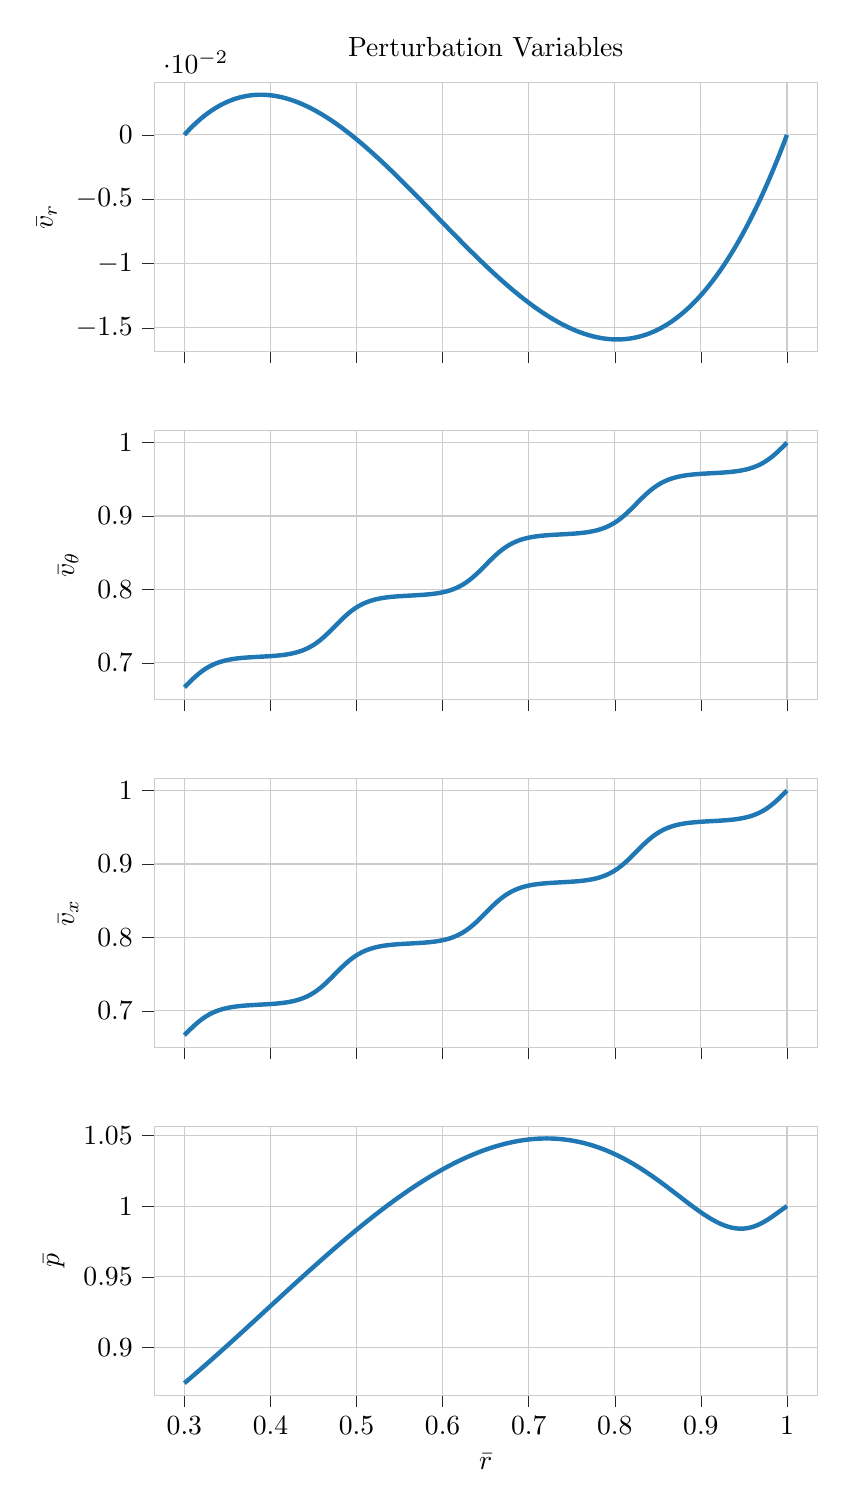
\begin{tikzpicture}

\definecolor{color0}{rgb}{0.12156862745098,0.466666666666667,0.705882352941177}

\begin{groupplot}[group style={group size=1 by 4}]
\nextgroupplot[
axis line style={white!80!black},
height=5cm,
scaled x ticks=manual:{}{\pgfmathparse{#1}},
tick align=outside,
tick pos=left,
title={Perturbation Variables},
width=10cm,
x grid style={white!80!black},
xmajorgrids,
xmin=0.265, xmax=1.035,
xtick style={color=white!15!black},
xticklabels={},
y grid style={white!80!black},
ylabel={\(\displaystyle \bar{v}_r\)},
ymajorgrids,
ymin=-0.0168534972835158, ymax=0.00407214087882566,
ytick style={color=white!15!black}
]
\addplot [ultra thick, color0]
table {%
0.3 0
0.30068093385214 5.08346872648974e-05
0.30136186770428 0.000101205659807119
0.30204280155642 0.000151114040603098
0.30272373540856 0.000200560952553719
0.3034046692607 0.000249547518483634
0.30408560311284 0.000298074861140502
0.304766536964981 0.000346144103194598
0.305447470817121 0.000393756367238068
0.306128404669261 0.000440912775784327
0.306809338521401 0.000487614451267479
0.307490272373541 0.000533862516041664
0.308171206225681 0.000579658092380475
0.308852140077821 0.000625002302476335
0.309533073929961 0.000669896268439829
0.310214007782101 0.000714341112299122
0.310894941634241 0.000758337955999361
0.311575875486381 0.000801887921401942
0.312256809338521 0.000844992130284008
0.312937743190661 0.000887651704337772
0.313618677042802 0.000929867765169845
0.314299610894942 0.000971641434300632
0.314980544747082 0.0010129738331638
0.315661478599222 0.00105386608310545
0.316342412451362 0.00109431930538362
0.317023346303502 0.00113433462116762
0.317704280155642 0.00117391315153736
0.318385214007782 0.00121305601748277
0.319066147859922 0.00125176433990311
0.319747081712062 0.00129003923960634
0.320428015564202 0.00132788183730843
0.321108949416342 0.00136529325363287
0.321789883268483 0.0014022746091098
0.322470817120623 0.00143882702417553
0.323151750972763 0.00147495161917183
0.323832684824903 0.00151064951434532
0.324513618677043 0.00154592182984668
0.325194552529183 0.00158076968573022
0.325875486381323 0.00161519420195304
0.326556420233463 0.00164919649837442
0.327237354085603 0.00168277769475525
0.327918287937743 0.00171593891075719
0.328599221789883 0.00174868126594221
0.329280155642023 0.00178100587977185
0.329961089494163 0.00181291387160648
0.330642023346304 0.0018444063607047
0.331322957198444 0.00187548446622272
0.332003891050584 0.00190614930721356
0.332684824902724 0.00193640200262661
0.333365758754864 0.00196624367130667
0.334046692607004 0.00199567543199344
0.334727626459144 0.00202469840332098
0.335408560311284 0.00205331370381674
0.336089494163424 0.00208152245190102
0.336770428015564 0.00210932576588638
0.337451361867704 0.00213672476397689
0.338132295719844 0.0021637205642674
0.338813229571985 0.00219031428474291
0.339494163424124 0.00221650704327787
0.340175097276265 0.00224229995763554
0.340856031128405 0.00226769414546732
0.341536964980545 0.00229269072431187
0.342217898832685 0.00231729081159472
0.342898832684825 0.0023414955246274
0.343579766536965 0.00236530598060666
0.344260700389105 0.00238872329661406
0.344941634241245 0.00241174858961507
0.345622568093385 0.00243438297645834
0.346303501945525 0.00245662757387517
0.346984435797665 0.00247848349847873
0.347665369649805 0.00249995186676329
0.348346303501946 0.00252103379510368
0.349027237354086 0.00254173039975449
0.349708171206226 0.0025620427968493
0.350389105058366 0.00258197210240012
0.351070038910506 0.00260151943229664
0.351750972762646 0.00262068590230546
0.352431906614786 0.00263947262806945
0.353112840466926 0.00265788072510706
0.353793774319066 0.00267591130881149
0.354474708171206 0.00269356549445013
0.355155642023346 0.00271084439716374
0.355836575875487 0.00272774913196583
0.356517509727627 0.00274428081374178
0.357198443579767 0.00276044055724843
0.357879377431907 0.00277622947711294
0.358560311284047 0.00279164868783241
0.359241245136187 0.00280669930377316
0.359922178988327 0.00282138243916968
0.360603112840467 0.00283569920812432
0.361284046692607 0.00284965072460626
0.361964980544747 0.00286323810245093
0.362645914396887 0.0028764624553593
0.363326848249027 0.00288932489689708
0.364007782101167 0.00290182654049399
0.364688715953307 0.0029139684994431
0.365369649805448 0.00292575188690007
0.366050583657588 0.00293717781588239
0.366731517509728 0.00294824739926866
0.367412451361868 0.00295896174979787
0.368093385214008 0.00296932198006868
0.368774319066148 0.00297932920253868
0.369455252918288 0.00298898452952355
0.370136186770428 0.00299828907319652
0.370817120622568 0.00300724394558742
0.371498054474708 0.0030158502585821
0.372178988326848 0.00302410912392156
0.372859922178988 0.00303202165320142
0.373540856031128 0.00303958895787082
0.374221789883268 0.00304681214923205
0.374902723735409 0.00305369233843955
0.375583657587549 0.00306023063649928
0.376264591439689 0.00306642815426794
0.376945525291829 0.00307228600245217
0.377626459143969 0.00307780529160795
0.378307392996109 0.00308298713213966
0.378988326848249 0.00308783263429943
0.379669260700389 0.0030923429081864
0.380350194552529 0.00309651906374594
0.381031128404669 0.00310036221076884
0.381712062256809 0.00310387345889063
0.38239299610895 0.00310705391759078
0.38307392996109 0.00310990469619198
0.38375486381323 0.00311242690385934
0.38443579766537 0.00311462164959961
0.38511673151751 0.00311649004226049
0.38579766536965 0.00311803319052981
0.38647859922179 0.00311925220293477
0.38715953307393 0.00312014818784119
0.38784046692607 0.00312072225345271
0.38852140077821 0.00312097550781014
0.38920233463035 0.00312090905879048
0.38988326848249 0.00312052401410631
0.39056420233463 0.00311982148130505
0.39124513618677 0.003118802567768
0.391926070038911 0.00311746838070982
0.392607003891051 0.00311582002717747
0.393287937743191 0.00311385861404968
0.393968871595331 0.00311158524803608
0.394649805447471 0.00310900103567639
0.395330739299611 0.00310610708333969
0.396011673151751 0.00310290449722359
0.396692607003891 0.00309939438335356
0.397373540856031 0.00309557784758199
0.398054474708171 0.00309145599558759
0.398735408560311 0.00308702993287444
0.399416342412451 0.00308230076477128
0.400097276264592 0.00307726959643079
0.400778210116732 0.00307193753282863
0.401459143968872 0.00306630567876288
0.402140077821012 0.00306037513885304
0.402821011673152 0.00305414701753938
0.403501945525292 0.00304762241908214
0.404182879377432 0.00304080244756065
0.404863813229572 0.00303368820687262
0.405544747081712 0.00302628080073335
0.406225680933852 0.00301858133267487
0.406906614785992 0.00301059090604522
0.407587548638132 0.00300231062400767
0.408268482490272 0.00299374158953979
0.408949416342412 0.00298488490543282
0.409630350194553 0.00297574167429077
0.410311284046693 0.00296631299852963
0.410992217898833 0.00295659998037667
0.411673151750973 0.0029466037218695
0.412354085603113 0.00293632532485537
0.413035019455253 0.00292576589099029
0.413715953307393 0.00291492652173834
0.414396887159533 0.00290380831837075
0.415077821011673 0.00289241238196519
0.415758754863813 0.00288073981340489
0.416439688715953 0.00286879171337789
0.417120622568093 0.00285656918237623
0.417801556420233 0.0028440733206951
0.418482490272374 0.00283130522843208
0.419163424124514 0.00281826600548633
0.419844357976654 0.00280495675155776
0.420525291828794 0.00279137856614621
0.421206225680934 0.0027775325485507
0.421887159533074 0.00276341979786851
0.422568093385214 0.00274904141299456
0.423249027237354 0.00273439849262036
0.423929961089494 0.00271949213523336
0.424610894941634 0.00270432343911613
0.425291828793774 0.00268889350234544
0.425972762645914 0.00267320342279158
0.426653696498055 0.00265725429811744
0.427334630350195 0.00264104722577775
0.428015564202335 0.0026245833030183
0.428696498054475 0.00260786362687493
0.429377431906615 0.00259088929417303
0.430058365758755 0.00257366140152646
0.430739299610895 0.00255618104533677
0.431420233463035 0.00253844932179254
0.432101167315175 0.00252046732686839
0.432782101167315 0.00250223615632424
0.433463035019455 0.00248375690570443
0.434143968871595 0.00246503067033703
0.434824902723735 0.00244605854533284
0.435505836575875 0.00242684162558465
0.436186770428016 0.0024073810057665
0.436867704280156 0.00238767778033272
0.437548638132296 0.00236773304351719
0.438229571984436 0.00234754788933249
0.438910505836576 0.00232712341156904
0.439591439688716 0.00230646070379438
0.440272373540856 0.00228556085935222
0.440953307392996 0.00226442497136171
0.441634241245136 0.00224305413271648
0.442315175097276 0.00222144943608406
0.442996108949416 0.00219961197390474
0.443677042801557 0.00217754283839101
0.444357976653696 0.00215524312152657
0.445038910505837 0.00213271391506559
0.445719844357977 0.00210995631053175
0.446400778210117 0.00208697139921764
0.447081712062257 0.00206376027218373
0.447762645914397 0.00204032402025757
0.448443579766537 0.00201666373403303
0.449124513618677 0.00199278050386943
0.449805447470817 0.00196867541989071
0.450486381322957 0.0019443495719846
0.451167315175097 0.00191980404980181
0.451848249027237 0.00189503994275508
0.452529182879377 0.00187005834001858
0.453210116731518 0.00184486033052683
0.453891050583658 0.00181944700297403
0.454571984435798 0.00179381944581314
0.455252918287938 0.00176797874725516
0.455933852140078 0.00174192599526808
0.456614785992218 0.00171566227757629
0.457295719844358 0.00168918868165961
0.457976653696498 0.00166250629475247
0.458657587548638 0.00163561620384309
0.459338521400778 0.00160851949567262
0.460019455252918 0.00158121725673438
0.460700389105058 0.00155371057327289
0.461381322957198 0.00152600053128323
0.462062256809338 0.00149808821650999
0.462743190661479 0.0014699747144466
0.463424124513619 0.00144166111033435
0.464105058365759 0.00141314848916171
0.464785992217899 0.00138443793566338
0.465466926070039 0.0013555305343195
0.466147859922179 0.00132642736935477
0.466828793774319 0.00129712952473772
0.467509727626459 0.00126763808417971
0.468190661478599 0.00123795413113421
0.468871595330739 0.001208078748796
0.469552529182879 0.00117801302010016
0.47023346303502 0.00114775802772148
0.47091439688716 0.00111731485407332
0.4715953307393 0.00108668458130706
0.47227626459144 0.00105586829131113
0.47295719844358 0.00102486706571009
0.47363813229572 0.000993681985864012
0.47431906614786 0.000962314132867445
0.475 0.000930764587548649
0.47568093385214 0.000899034430468806
0.47636186770428 0.000867124741921119
0.47704280155642 0.000835036601929934
0.47772373540856 0.000802771090250065
0.4784046692607 0.00077032928636582
0.47908560311284 0.000737712269490168
0.479766536964981 0.00070492111856392
0.480447470817121 0.000671956912255009
0.481128404669261 0.000638820728957504
0.481809338521401 0.00060551364679072
0.482490272373541 0.000572036743598681
0.483171206225681 0.000538391096948893
0.483852140077821 0.000504577784131904
0.484533073929961 0.000470597882160098
0.485214007782101 0.000436452467767107
0.485894941634241 0.000402142617406925
0.486575875486381 0.000367669407252982
0.487256809338522 0.000333033913197472
0.487937743190662 0.000298237210850372
0.488618677042802 0.000263280375538633
0.489299610894942 0.000228164482305421
0.489980544747082 0.000192890605909268
0.490661478599222 0.00015745982082313
0.491342412451362 0.000121873201233663
0.492023346303502 8.61318210404194e-05
0.492704280155642 5.02367538548903e-05
0.493385214007782 1.41890729997984e-05
0.494066147859922 -2.20101484918467e-05
0.494747081712062 -5.83598378774697e-05
0.495428015564202 -9.48589227058316e-05
0.496108949416342 -0.000131506330817807
0.496789883268483 -0.000168300990347314
0.497470817120623 -0.000205241829722022
0.498151750972763 -0.000242327777664225
0.498832684824903 -0.000279557763191676
0.499513618677043 -0.000316930715618433
0.500194552529183 -0.000354445564555689
0.500875486381323 -0.000392101239912526
0.501556420233463 -0.000429896671896787
0.502237354085603 -0.000467830791016019
0.502918287937743 -0.000505902528078028
0.503599221789883 -0.000544110814191964
0.504280155642023 -0.000582454580769012
0.504961089494164 -0.000620932759523254
0.505642023346303 -0.00065954428247246
0.506322957198444 -0.000698288081938947
0.507003891050584 -0.000737163090550427
0.507684824902724 -0.000776168241240715
0.508365758754864 -0.000815302467250672
0.509046692607004 -0.000854564702128927
0.509727626459144 -0.000893953879732817
0.510408560311284 -0.000933468934229104
0.511089494163424 -0.000973108800094741
0.511770428015564 -0.00101287241211792
0.512451361867704 -0.00105275870539859
0.513132295719844 -0.00109276661534947
0.513813229571984 -0.00113289507769691
0.514494163424124 -0.00117314302848144
0.515175097276265 -0.00121350940405884
0.515856031128405 -0.00125399314110089
0.516536964980545 -0.00129459317659611
0.517217898832685 -0.00133530844785064
0.517898832684825 -0.00137613789248896
0.518579766536965 -0.00141708044845487
0.519260700389105 -0.0014581350540121
0.519941634241245 -0.00149930064774528
0.520622568093385 -0.00154057616856067
0.521303501945525 -0.00158196055568692
0.521984435797665 -0.00162345274867594
0.522665369649805 -0.00166505168740376
0.523346303501946 -0.00170675631207118
0.524027237354086 -0.0017485655632047
0.524708171206226 -0.00179047838165726
0.525389105058366 -0.00183249370860908
0.526070038910506 -0.00187461048556845
0.526750972762646 -0.00191682765437241
0.527431906614786 -0.00195914415718776
0.528112840466926 -0.00200155893651177
0.528793774319066 -0.00204407093517284
0.529474708171206 -0.00208667909633146
0.530155642023346 -0.00212938236348101
0.530836575875486 -0.00217217968044839
0.531517509727626 -0.00221506999139495
0.532198443579767 -0.00225805224081728
0.532879377431907 -0.00230112537354789
0.533560311284047 -0.00234428833475614
0.534241245136187 -0.00238754006994889
0.534922178988327 -0.00243087952497141
0.535603112840467 -0.00247430564600799
0.536284046692607 -0.00251781737958297
0.536964980544747 -0.0025614136725613
0.537645914396887 -0.00260509347214946
0.538326848249027 -0.00264885572589613
0.539007782101167 -0.00269269938169303
0.539688715953307 -0.00273662338777572
0.540369649805448 -0.00278062669272433
0.541050583657588 -0.00282470824546435
0.541731517509728 -0.00286886699526734
0.542412451361868 -0.00291310189175187
0.543093385214008 -0.00295741188488409
0.543774319066148 -0.00300179592497864
0.544455252918288 -0.00304625296269929
0.545136186770428 -0.00309078194905991
0.545817120622568 -0.00313538183542501
0.546498054474708 -0.00318005157351059
0.547178988326848 -0.00322479011538494
0.547859922178988 -0.00326959641346938
0.548540856031128 -0.00331446942053901
0.549221789883269 -0.00335940808972338
0.549902723735409 -0.00340441137450748
0.550583657587549 -0.00344947822873218
0.551264591439689 -0.00349460760659528
0.551945525291829 -0.00353979846265207
0.552626459143969 -0.00358504975181609
0.553307392996109 -0.00363036042936002
0.553988326848249 -0.00367572945091628
0.554669260700389 -0.00372115577247777
0.555350194552529 -0.00376663835039878
0.556031128404669 -0.00381217614139555
0.556712062256809 -0.00385776810254707
0.55739299610895 -0.00390341319129583
0.55807392996109 -0.00394911036544862
0.55875486381323 -0.00399485858317711
0.55943579766537 -0.00404065680301868
0.56011673151751 -0.00408650398387719
0.56079766536965 -0.00413239908502369
0.56147859922179 -0.00417834106609695
0.56215953307393 -0.00422432888710457
0.56284046692607 -0.0042703615084233
0.56352140077821 -0.00431643789080009
0.56420233463035 -0.00436255699535262
0.56488326848249 -0.00440871778357003
0.56556420233463 -0.00445491921731372
0.566245136186771 -0.00450116025881803
0.566926070038911 -0.00454743987069091
0.567607003891051 -0.00459375701591472
0.568287937743191 -0.00464011065784678
0.568968871595331 -0.00468649976022031
0.569649805447471 -0.00473292328714495
0.570330739299611 -0.00477938020310745
0.571011673151751 -0.00482586947297256
0.571692607003891 -0.00487239006198358
0.572373540856031 -0.00491894093576303
0.573054474708171 -0.00496552106031352
0.573735408560311 -0.0050121294020182
0.574416342412451 -0.00505876492764162
0.575097276264592 -0.00510542660433042
0.575778210116731 -0.00515211339961395
0.576459143968872 -0.00519882428140497
0.577140077821012 -0.00524555821800041
0.577821011673152 -0.00529231417808187
0.578501945525292 -0.00533909113071648
0.579182879377432 -0.00538588804535758
0.579863813229572 -0.00543270389184516
0.580544747081712 -0.00547953764040687
0.581225680933852 -0.00552638826165838
0.581906614785992 -0.0055732547266043
0.582587548638132 -0.00562013600663865
0.583268482490272 -0.00566703107354559
0.583949416342412 -0.00571393889950017
0.584630350194552 -0.00576085845706888
0.585311284046693 -0.00580778871921037
0.585992217898833 -0.00585472865927597
0.586673151750973 -0.00590167725101057
0.587354085603113 -0.00594863346855308
0.588035019455253 -0.00599559628643718
0.588715953307393 -0.0060425646795919
0.589396887159533 -0.00608953762334227
0.590077821011673 -0.00613651409341004
0.590758754863813 -0.00618349306591419
0.591439688715953 -0.00623047351737172
0.592120622568093 -0.00627745442469808
0.592801556420233 -0.006324434765208
0.593482490272374 -0.00637141351661603
0.594163424124514 -0.00641838965703712
0.594844357976654 -0.0064653621649873
0.595525291828794 -0.00651233001938435
0.596206225680934 -0.00655929219954829
0.596887159533074 -0.00660624768520207
0.597568093385214 -0.00665319545647222
0.598249027237354 -0.00670013449388936
0.598929961089494 -0.00674706377838891
0.599610894941634 -0.00679398229131162
0.600291828793774 -0.00684088901440418
0.600972762645914 -0.00688778292981983
0.601653696498054 -0.00693466302011905
0.602334630350195 -0.00698152826826999
0.603015564202335 -0.00702837765764915
0.603696498054475 -0.00707521017204194
0.604377431906615 -0.00712202479564331
0.605058365758755 -0.0071688205130583
0.605739299610895 -0.0072155963093026
0.606420233463035 -0.00726235116980321
0.607101167315175 -0.0073090840803989
0.607782101167315 -0.00735579402734085
0.608463035019455 -0.0074024799972932
0.609143968871595 -0.00744914097733362
0.609824902723735 -0.00749577595495393
0.610505836575876 -0.00754238391806053
0.611186770428016 -0.00758896385497504
0.611867704280156 -0.0076355147544349
0.612548638132296 -0.00768203560559383
0.613229571984436 -0.00772852539802241
0.613910505836576 -0.00777498312170866
0.614591439688716 -0.00782140776705847
0.615272373540856 -0.00786779832489636
0.615953307392996 -0.00791415378646579
0.616634241245136 -0.00796047314342976
0.617315175097276 -0.00800675538787143
0.617996108949416 -0.00805299951229455
0.618677042801557 -0.00809920450962398
0.619357976653697 -0.0081453693732063
0.620038910505837 -0.00819149309681025
0.620719844357977 -0.00823757467462724
0.621400778210117 -0.00828361310127193
0.622081712062257 -0.00832960737178268
0.622762645914397 -0.00837555648162205
0.623443579766537 -0.00842145942667738
0.624124513618677 -0.00846731520326119
0.624805447470817 -0.0085131228081117
0.625486381322957 -0.00855888123839341
0.626167315175097 -0.0086045894916974
0.626848249027237 -0.0086502465660421
0.627529182879378 -0.00869585145987348
0.628210116731518 -0.00874140317206568
0.628891050583658 -0.00878690070192154
0.629571984435798 -0.00883234304917285
0.630252918287938 -0.00887772921398114
0.630933852140078 -0.00892305819693781
0.631614785992218 -0.00896832899906486
0.632295719844358 -0.00901354062181522
0.632976653696498 -0.0090586920670732
0.633657587548638 -0.00910378233715498
0.634338521400778 -0.00914881043480907
0.635019455252918 -0.00919377536321669
0.635700389105058 -0.00923867612599233
0.636381322957199 -0.00928351172718402
0.637062256809338 -0.00932828117127393
0.637743190661479 -0.00937298346317873
0.638424124513619 -0.00941761760824997
0.639105058365759 -0.00946218261227457
0.639785992217899 -0.00950667748147524
0.640466926070039 -0.00955110122251088
0.641147859922179 -0.00959545284247698
0.641828793774319 -0.009639731348906
0.642509727626459 -0.00968393574976797
0.643190661478599 -0.00972806505347054
0.643871595330739 -0.00977211826885971
0.644552529182879 -0.00981609440522012
0.645233463035019 -0.00985999247227526
0.645914396887159 -0.00990381148018821
0.6465953307393 -0.00994755043956166
0.64727626459144 -0.00999120836143858
0.64795719844358 -0.0100347842573024
0.64863813229572 -0.0100782771390776
0.64931906614786 -0.0101216860191296
0.65 -0.0101650099102659
0.65068093385214 -0.0102082478257358
0.65136186770428 -0.0102513987792308
0.65204280155642 -0.0102944617848854
0.65272373540856 -0.010337435857277
0.6534046692607 -0.0103803200114265
0.65408560311284 -0.0104231132627984
0.654766536964981 -0.0104658146273014
0.655447470817121 -0.0105084231212887
0.656128404669261 -0.0105509377615582
0.656809338521401 -0.0105933575653529
0.657490272373541 -0.010635681550361
0.658171206225681 -0.0106779087347168
0.658852140077821 -0.0107200381370002
0.659533073929961 -0.0107620687762379
0.660214007782101 -0.0108039996719029
0.660894941634241 -0.0108458298439154
0.661575875486381 -0.0108875583126427
0.662256809338521 -0.0109291840988996
0.662937743190661 -0.0109707062239491
0.663618677042802 -0.0110121237095018
0.664299610894942 -0.0110534355777172
0.664980544747082 -0.0110946408512032
0.665661478599222 -0.0111357385530166
0.666342412451362 -0.0111767277066638
0.667023346303502 -0.0112176073361002
0.667704280155642 -0.0112583764657315
0.668385214007782 -0.0112990341204129
0.669066147859922 -0.0113395793254502
0.669747081712062 -0.0113800111065996
0.670428015564202 -0.0114203284900681
0.671108949416342 -0.0114605305025137
0.671789883268483 -0.0115006161710455
0.672470817120623 -0.0115405845232243
0.673151750972763 -0.0115804345870625
0.673832684824903 -0.0116201653910243
0.674513618677043 -0.0116597759640263
0.675194552529183 -0.0116992653354371
0.675875486381323 -0.0117386325350782
0.676556420233463 -0.0117778765932237
0.677237354085603 -0.0118169965406006
0.677918287937743 -0.0118559914083893
0.678599221789883 -0.0118948602282234
0.679280155642023 -0.0119336020321901
0.679961089494163 -0.0119722158528302
0.680642023346304 -0.0120107007231386
0.681322957198444 -0.0120490556765642
0.682003891050584 -0.0120872797470101
0.682684824902724 -0.012125371968834
0.683365758754864 -0.0121633313768481
0.684046692607004 -0.0122011570063191
0.684727626459144 -0.0122388478929691
0.685408560311284 -0.0122764030729747
0.686089494163424 -0.0123138215829681
0.686770428015564 -0.0123511024600366
0.687451361867704 -0.012388244741723
0.688132295719844 -0.0124252474660258
0.688813229571985 -0.0124621096713991
0.689494163424125 -0.0124988303967528
0.690175097276265 -0.0125354086814529
0.690856031128405 -0.0125718435653214
0.691536964980545 -0.0126081340886364
0.692217898832685 -0.0126442792921322
0.692898832684825 -0.0126802782169999
0.693579766536965 -0.0127161299048865
0.694260700389105 -0.0127518333978958
0.694941634241245 -0.0127873877385884
0.695622568093385 -0.0128227919699814
0.696303501945525 -0.0128580451355486
0.696984435797665 -0.012893146279221
0.697665369649806 -0.0129280944453861
0.698346303501946 -0.0129628886788888
0.699027237354086 -0.0129975280250307
0.699708171206226 -0.0130320115295706
0.700389105058366 -0.0130663382387246
0.701070038910506 -0.0131005071991656
0.701750972762646 -0.0131345174580241
0.702431906614786 -0.0131683680628876
0.703112840466926 -0.0132020580618009
0.703793774319066 -0.0132355865032661
0.704474708171206 -0.0132689524362427
0.705155642023346 -0.0133021549101474
0.705836575875486 -0.0133351929748542
0.706517509727627 -0.0133680656806946
0.707198443579766 -0.0134007720784571
0.707879377431907 -0.0134333112193878
0.708560311284047 -0.0134656821551901
0.709241245136187 -0.0134978839380244
0.709922178988327 -0.0135299156205087
0.710603112840467 -0.0135617762557181
0.711284046692607 -0.0135934648971847
0.711964980544747 -0.013624980598898
0.712645914396887 -0.0136563224153047
0.713326848249027 -0.0136874894013082
0.714007782101167 -0.0137184806122694
0.714688715953307 -0.0137492951040056
0.715369649805447 -0.0137799319327916
0.716050583657587 -0.0138103901553585
0.716731517509728 -0.0138406688288945
0.717412451361868 -0.0138707670110444
0.718093385214008 -0.0139006837599095
0.718774319066148 -0.0139304181340476
0.719455252918288 -0.0139599691924732
0.720136186770428 -0.0139893359946568
0.720817120622568 -0.0140185176005252
0.721498054474708 -0.0140475130704614
0.722178988326848 -0.0140763214653043
0.722859922178988 -0.0141049418463487
0.723540856031128 -0.0141333732753451
0.724221789883268 -0.0141616148144998
0.724902723735409 -0.0141896655264745
0.725583657587549 -0.014217524474386
0.726264591439689 -0.0142451907218068
0.726945525291829 -0.014272663332764
0.727626459143969 -0.0142999413717399
0.728307392996109 -0.0143270239036713
0.728988326848249 -0.0143539099939499
0.729669260700389 -0.0143805987084214
0.730350194552529 -0.0144070891133862
0.731031128404669 -0.0144333802755983
0.73171206225681 -0.0144594712622659
0.732392996108949 -0.0144853611410507
0.73307392996109 -0.0145110489800679
0.73375486381323 -0.014536533847886
0.73443579766537 -0.0145618148135267
0.73511673151751 -0.0145868909464643
0.73579766536965 -0.014611761316626
0.73647859922179 -0.0146364249943912
0.73715953307393 -0.0146608810505916
0.73784046692607 -0.0146851285565109
0.73852140077821 -0.0147091665838844
0.73920233463035 -0.014732994204899
0.73988326848249 -0.0147566104921928
0.74056420233463 -0.0147800145188548
0.74124513618677 -0.0148032053584247
0.741926070038911 -0.0148261820848929
0.742607003891051 -0.0148489437726996
0.743287937743191 -0.0148714894967351
0.743968871595331 -0.0148938183323394
0.744649805447471 -0.0149159293553017
0.745330739299611 -0.0149378216418603
0.746011673151751 -0.0149594942687022
0.746692607003891 -0.0149809463129629
0.747373540856031 -0.015002176852226
0.748054474708171 -0.015023184964523
0.748735408560311 -0.0150439697283326
0.749416342412451 -0.0150645302225812
0.750097276264592 -0.0150848655266416
0.750778210116732 -0.0151049747203333
0.751459143968872 -0.015124856883922
0.752140077821012 -0.0151445110981191
0.752821011673152 -0.0151639364440815
0.753501945525292 -0.0151831320034115
0.754182879377432 -0.0152020968581557
0.754863813229572 -0.0152208300908054
0.755544747081712 -0.0152393307842959
0.756225680933852 -0.015257598022006
0.756906614785992 -0.0152756308877579
0.757587548638132 -0.0152934284658166
0.758268482490272 -0.0153109898408894
0.758949416342413 -0.0153283140981261
0.759630350194553 -0.0153454003231177
0.760311284046693 -0.0153622476018968
0.760992217898833 -0.0153788550209366
0.761673151750973 -0.0153952216671509
0.762354085603113 -0.0154113466278934
0.763035019455253 -0.0154272289909572
0.763715953307393 -0.0154428678445748
0.764396887159533 -0.0154582622774173
0.765077821011673 -0.0154734113785938
0.765758754863813 -0.0154883142376515
0.766439688715953 -0.0155029699445746
0.767120622568093 -0.0155173775897843
0.767801556420234 -0.0155315362641383
0.768482490272373 -0.0155454450589299
0.769163424124514 -0.015559103065888
0.769844357976654 -0.0155725093771762
0.770525291828794 -0.0155856630853929
0.771206225680934 -0.0155985632835702
0.771887159533074 -0.0156112090651736
0.772568093385214 -0.0156235995241016
0.773249027237354 -0.015635733754685
0.773929961089494 -0.0156476108516866
0.774610894941634 -0.0156592299103004
0.775291828793774 -0.0156705900261514
0.775972762645914 -0.0156816902952947
0.776653696498054 -0.0156925298142153
0.777334630350194 -0.0157031076798272
0.778015564202335 -0.0157134229894732
0.778696498054475 -0.0157234748409241
0.779377431906615 -0.0157332623323782
0.780058365758755 -0.0157427845624608
0.780739299610895 -0.0157520406302235
0.781420233463035 -0.0157610296351436
0.782101167315175 -0.0157697506771237
0.782782101167315 -0.0157782028564911
0.783463035019455 -0.0157863852739968
0.784143968871595 -0.0157942970308155
0.784824902723735 -0.0158019372285446
0.785505836575875 -0.0158093049692034
0.786186770428016 -0.0158163993552331
0.786867704280156 -0.0158232194894957
0.787548638132296 -0.0158297644752735
0.788229571984436 -0.0158360334162683
0.788910505836576 -0.0158420254166012
0.789591439688716 -0.0158477395808113
0.790272373540856 -0.0158531750138558
0.790953307392996 -0.0158583308211087
0.791634241245136 -0.0158632061083603
0.792315175097276 -0.0158677999818169
0.792996108949416 -0.0158721115480996
0.793677042801556 -0.015876139914244
0.794357976653696 -0.0158798841876993
0.795038910505837 -0.0158833434763275
0.795719844357977 -0.0158865168884032
0.796400778210117 -0.0158894035326124
0.797081712062257 -0.015892002518052
0.797762645914397 -0.015894312954229
0.798443579766537 -0.0158963339510597
0.799124513618677 -0.0158980646188695
0.799805447470817 -0.0158995040683914
0.800486381322957 -0.0159006514107658
0.801167315175097 -0.0159015057575395
0.801848249027237 -0.0159020662206651
0.802529182879377 -0.0159023319125003
0.803210116731518 -0.0159023019458067
0.803891050583658 -0.0159019754337498
0.804571984435798 -0.0159013514898973
0.805252918287938 -0.0159004292282194
0.805933852140078 -0.015899207763087
0.806614785992218 -0.0158976862092715
0.807295719844358 -0.0158958636819438
0.807976653696498 -0.0158937392966737
0.808657587548638 -0.0158913121694289
0.809338521400778 -0.0158885814165742
0.810019455252918 -0.0158855461548709
0.810700389105058 -0.0158822055014755
0.811381322957198 -0.0158785585739396
0.812062256809339 -0.0158746044902085
0.812743190661479 -0.0158703423686203
0.813424124513619 -0.0158657713279057
0.814105058365759 -0.0158608904871865
0.814785992217899 -0.0158556989659752
0.815466926070039 -0.0158501958841736
0.816147859922179 -0.0158443803620725
0.816828793774319 -0.0158382515203506
0.817509727626459 -0.0158318084800737
0.818190661478599 -0.0158250503626937
0.818871595330739 -0.0158179762900476
0.819552529182879 -0.0158105853843571
0.82023346303502 -0.0158028767682272
0.82091439688716 -0.0157948495646456
0.8215953307393 -0.0157865028969814
0.82227626459144 -0.0157778358889848
0.82295719844358 -0.0157688476647859
0.82363813229572 -0.0157595373488935
0.82431906614786 -0.0157499040661944
0.825 -0.0157399469419527
0.82568093385214 -0.0157296651018085
0.82636186770428 -0.0157190576717772
0.82704280155642 -0.0157081237782483
0.82772373540856 -0.0156968625479848
0.828404669260701 -0.0156852731081218
0.829085603112841 -0.015673354586166
0.829766536964981 -0.0156611061099944
0.830447470817121 -0.0156485268078535
0.831128404669261 -0.0156356158083581
0.831809338521401 -0.0156223722404908
0.832490272373541 -0.0156087952336003
0.833171206225681 -0.015594883917401
0.833852140077821 -0.0155806374219718
0.834533073929961 -0.015566054877755
0.835214007782101 -0.0155511354155554
0.835894941634241 -0.0155358781665393
0.836575875486381 -0.0155202822622335
0.837256809338522 -0.0155043468345238
0.837937743190662 -0.015488071015655
0.838618677042802 -0.0154714539382288
0.839299610894942 -0.0154544947352033
0.839980544747082 -0.015437192539892
0.840661478599222 -0.0154195464859624
0.841342412451362 -0.0154015557074352
0.842023346303502 -0.0153832193386833
0.842704280155642 -0.0153645365144305
0.843385214007782 -0.0153455063697506
0.844066147859922 -0.0153261280400662
0.844747081712062 -0.0153064006611478
0.845428015564202 -0.0152863233691124
0.846108949416343 -0.0152658953004229
0.846789883268482 -0.0152451155918864
0.847470817120623 -0.0152239833806537
0.848151750972763 -0.0152024978042176
0.848832684824903 -0.0151806580004123
0.849513618677043 -0.015158463107412
0.850194552529183 -0.0151359122637298
0.850875486381323 -0.0151130046082168
0.851556420233463 -0.0150897392800606
0.852237354085603 -0.0150661154187844
0.852918287937743 -0.0150421321642458
0.853599221789883 -0.0150177886566357
0.854280155642023 -0.0149930840364771
0.854961089494163 -0.0149680174446239
0.855642023346303 -0.0149425880222599
0.856322957198444 -0.0149167949108975
0.857003891050584 -0.0148906372523764
0.857684824902724 -0.0148641141888628
0.858365758754864 -0.0148372248628479
0.859046692607004 -0.0148099684171469
0.859727626459144 -0.0147823439948974
0.860408560311284 -0.0147543507395589
0.861089494163424 -0.0147259877949112
0.861770428015564 -0.0146972543050529
0.862451361867704 -0.014668149414401
0.863132295719844 -0.0146386722676887
0.863813229571984 -0.014608822009965
0.864494163424125 -0.014578597786593
0.865175097276265 -0.014547998743249
0.865856031128405 -0.014517024025921
0.866536964980545 -0.0144856727809076
0.867217898832685 -0.0144539441548165
0.867898832684825 -0.0144218372945639
0.868579766536965 -0.0143893513473723
0.869260700389105 -0.0143564854607702
0.869941634241245 -0.0143232387825903
0.870622568093385 -0.0142896104609681
0.871303501945525 -0.0142555996443411
0.871984435797665 -0.0142212054814474
0.872665369649805 -0.014186427121324
0.873346303501946 -0.014151263713306
0.874027237354086 -0.0141157144070252
0.874708171206226 -0.0140797783524087
0.875389105058366 -0.0140434546996777
0.876070038910506 -0.014006742599346
0.876750972762646 -0.0139696412022191
0.877431906614786 -0.0139321496593924
0.878112840466926 -0.0138942671222503
0.878793774319066 -0.0138559927424646
0.879474708171206 -0.0138173256719935
0.880155642023346 -0.0137782650630797
0.880836575875486 -0.0137388100682499
0.881517509727627 -0.0136989598403124
0.882198443579767 -0.0136587135323569
0.882879377431907 -0.0136180702977524
0.883560311284047 -0.0135770292901461
0.884241245136187 -0.0135355896634618
0.884922178988327 -0.0134937505718991
0.885603112840467 -0.0134515111699313
0.886284046692607 -0.013408870612305
0.886964980544747 -0.0133658280540375
0.887645914396887 -0.0133223826504165
0.888326848249027 -0.0132785335569982
0.889007782101167 -0.013234279929606
0.889688715953307 -0.0131896209243293
0.890369649805448 -0.0131445556975216
0.891050583657588 -0.0130990834057999
0.891731517509728 -0.0130532032060425
0.892412451361868 -0.0130069142553881
0.893093385214008 -0.0129602157112343
0.893774319066148 -0.0129131067312361
0.894455252918288 -0.0128655864733044
0.895136186770428 -0.012817654095605
0.895817120622568 -0.0127693087565566
0.896498054474708 -0.0127205496148298
0.897178988326848 -0.0126713758293455
0.897859922178988 -0.0126217865592736
0.898540856031128 -0.0125717809640314
0.899221789883269 -0.0125213582032821
0.899902723735409 -0.0124705174369336
0.900583657587549 -0.012419257825137
0.901264591439689 -0.012367578528285
0.901945525291829 -0.0123154787070104
0.902626459143969 -0.0122629575221851
0.903307392996109 -0.0122100141349179
0.903988326848249 -0.0121566477065538
0.904669260700389 -0.0121028573986718
0.905350194552529 -0.0120486423730841
0.906031128404669 -0.0119940017918342
0.906712062256809 -0.0119389348171955
0.90739299610895 -0.0118834406116699
0.90807392996109 -0.0118275183379861
0.90875486381323 -0.0117711671590986
0.90943579766537 -0.0117143862381855
0.91011673151751 -0.0116571747386476
0.91079766536965 -0.0115995318241066
0.91147859922179 -0.0115414566584037
0.91215953307393 -0.0114829484055979
0.91284046692607 -0.0114240062299649
0.91352140077821 -0.0113646292959952
0.91420233463035 -0.0113048167683926
0.91488326848249 -0.011244567812073
0.91556420233463 -0.0111838815921624
0.91624513618677 -0.0111227572739959
0.91692607003891 -0.0110611940231157
0.917607003891051 -0.0109991910052699
0.918287937743191 -0.0109367473864106
0.918968871595331 -0.0108738623326929
0.919649805447471 -0.0108105350104727
0.920330739299611 -0.0107467645863058
0.921011673151751 -0.0106825502269458
0.921692607003891 -0.010617891099343
0.922373540856031 -0.0105527863706422
0.923054474708171 -0.0104872352081822
0.923735408560311 -0.0104212367794929
0.924416342412451 -0.0103547902522951
0.925097276264591 -0.0102878947944977
0.925778210116732 -0.0102205495741971
0.926459143968872 -0.0101527537596748
0.927140077821012 -0.0100845065193968
0.927821011673152 -0.0100158070220109
0.928501945525292 -0.00994665443634586
0.929182879377432 -0.00987704793140987
0.929863813229572 -0.00980698667638831
0.930544747081712 -0.00973646984064282
0.931225680933852 -0.00966549659370936
0.931906614785992 -0.00959406610529666
0.932587548638132 -0.00952217754528481
0.933268482490272 -0.00944983008372323
0.933949416342412 -0.00937702289082962
0.934630350194552 -0.00930375513698781
0.935311284046693 -0.00923002599274664
0.935992217898833 -0.00915583462881789
0.936673151750973 -0.00908118021607506
0.937354085603113 -0.0090060619255514
0.938035019455253 -0.00893047892843864
0.938715953307393 -0.00885443039608508
0.939396887159533 -0.00877791549999403
0.940077821011673 -0.00870093341182232
0.940758754863813 -0.00862348330337855
0.941439688715953 -0.00854556434662133
0.942120622568093 -0.00846717571365799
0.942801556420233 -0.00838831657674261
0.943482490272374 -0.00830898610827455
0.944163424124514 -0.00822918348079674
0.944844357976654 -0.00814890786699407
0.945525291828794 -0.00806815843969171
0.946206225680934 -0.00798693437185352
0.946887159533074 -0.00790523483658026
0.947568093385214 -0.00782305900710818
0.948249027237354 -0.00774040605680709
0.948929961089494 -0.00765727515917883
0.949610894941634 -0.00757366548785565
0.950291828793774 -0.00748957621659856
0.950972762645914 -0.00740500651929538
0.951653696498054 -0.00731995556995954
0.952334630350194 -0.00723442254272805
0.953015564202334 -0.00714840661185998
0.953696498054475 -0.00706190695173474
0.954377431906615 -0.00697492273685035
0.955058365758755 -0.00688745314182196
0.955739299610895 -0.00679949734138002
0.956420233463035 -0.00671105451036851
0.957101167315175 -0.00662212382374352
0.957782101167315 -0.00653270445657121
0.958463035019455 -0.00644279558402652
0.959143968871595 -0.00635239638139128
0.959824902723735 -0.00626150602405243
0.960505836575875 -0.00617012368750045
0.961186770428015 -0.00607824854732769
0.961867704280156 -0.00598587977922657
0.962548638132296 -0.00589301655898804
0.963229571984436 -0.00579965806249977
0.963910505836576 -0.00570580346574438
0.964591439688716 -0.00561145194479791
0.965272373540856 -0.00551660267582803
0.965953307392996 -0.00542125483509229
0.966634241245136 -0.00532540759893652
0.967315175097276 -0.00522906014379306
0.967996108949416 -0.00513221164617905
0.968677042801556 -0.00503486128269476
0.969357976653697 -0.0049370082300219
0.970038910505837 -0.00483865166492159
0.970719844357977 -0.00473979076423332
0.971400778210117 -0.00464042470487261
0.972081712062257 -0.00454055266382952
0.972762645914397 -0.00444017381816691
0.973443579766537 -0.00433928734501886
0.974124513618677 -0.00423789242158876
0.974805447470817 -0.00413598822514766
0.975486381322957 -0.00403357393303252
0.976167315175097 -0.00393064872264466
0.976848249027237 -0.00382721177144772
0.977529182879378 -0.0037232622569662
0.978210116731518 -0.00361879935678366
0.978891050583658 -0.00351382224854103
0.979571984435798 -0.00340833010993459
0.980252918287938 -0.00330232211871483
0.980933852140078 -0.0031957974526841
0.981614785992218 -0.00308875528969525
0.982295719844358 -0.00298119480764991
0.982976653696498 -0.00287311518449647
0.983657587548638 -0.00276451559822873
0.984338521400778 -0.00265539522688368
0.985019455252918 -0.00254575324854037
0.985700389105058 -0.00243558884131777
0.986381322957199 -0.00232490118337292
0.987062256809339 -0.00221368945289963
0.987743190661479 -0.00210195282812647
0.988424124513619 -0.00198969048731507
0.989105058365759 -0.00187690160875828
0.989785992217899 -0.00176358537077874
0.990466926070039 -0.00164974095172676
0.991147859922179 -0.00153536752997889
0.991828793774319 -0.00142046428393594
0.992509727626459 -0.00130503039202151
0.993190661478599 -0.00118906503267996
0.993871595330739 -0.00107256738437486
0.99455252918288 -0.000955536625587228
0.99523346303502 -0.000837971934813678
0.99591439688716 -0.000719872490564821
0.9965953307393 -0.000601237471363439
0.99727626459144 -0.000482066055742761
0.99795719844358 -0.000362357422244733
0.99863813229572 -0.000242110749418364
0.99931906614786 -0.000121325215817619
1 -2.77555756156289e-16
};

\nextgroupplot[
axis line style={white!80!black},
height=5cm,
scaled x ticks=manual:{}{\pgfmathparse{#1}},
tick align=outside,
tick pos=left,
width=10cm,
x grid style={white!80!black},
xmajorgrids,
xmin=0.265, xmax=1.035,
xtick style={color=white!15!black},
xticklabels={},
y grid style={white!80!black},
ylabel={\(\displaystyle \bar{v}_{\theta}\)},
ymajorgrids,
ymin=0.650007944987741, ymax=1.01666628833392,
ytick style={color=white!15!black}
]
\addplot [ultra thick, color0]
table {%
0.3 0.666674233321658
0.30068093385214 0.667484916704007
0.30136186770428 0.668294992843608
0.30204280155642 0.669103850632943
0.30272373540856 0.669910882670412
0.3034046692607 0.670715487079348
0.30408560311284 0.671517069291871
0.304766536964981 0.672315043786443
0.305447470817121 0.673108835768496
0.306128404669261 0.673897882784138
0.306809338521401 0.674681636257611
0.307490272373541 0.675459562944024
0.308171206225681 0.67623114628972
0.308852140077821 0.67699588769359
0.309533073929961 0.677753307663636
0.310214007782101 0.678502946864106
0.310894941634241 0.679244367049533
0.311575875486381 0.679977151883095
0.312256809338521 0.680700907637711
0.312937743190661 0.681415263779319
0.313618677042802 0.682119873432732
0.314299610894942 0.682814413731424
0.314980544747082 0.683498586053466
0.315661478599222 0.684172116146606
0.316342412451362 0.684834754146287
0.317023346303502 0.685486274491002
0.317704280155642 0.686126475740005
0.318385214007782 0.686755180298879
0.319066147859922 0.687372234058886
0.319747081712062 0.687977505956354
0.320428015564202 0.688570887458613
0.321108949416342 0.689152291983167
0.321789883268483 0.689721654256879
0.322470817120623 0.690278929621987
0.323151750972763 0.690824093295712
0.323832684824903 0.691357139590154
0.324513618677043 0.691878081098973
0.325194552529183 0.692386947857196
0.325875486381323 0.692883786480221
0.326556420233463 0.693368659287819
0.327237354085603 0.693841643418626
0.327918287937743 0.694302829940296
0.328599221789883 0.694752322960109
0.329280155642023 0.695190238740502
0.329961089494163 0.695616704823596
0.330642023346304 0.696031859168431
0.331322957198444 0.696435849304246
0.332003891050584 0.696828831502775
0.332684824902724 0.697210969972188
0.333365758754864 0.697582436074919
0.334046692607004 0.697943407571354
0.334727626459144 0.698294067890957
0.335408560311284 0.698634605432185
0.336089494163424 0.698965212892212
0.336770428015564 0.699286086627224
0.337451361867704 0.69959742604383
0.338132295719844 0.699899433021879
0.338813229571985 0.700192311368776
0.339494163424124 0.700476266305212
0.340175097276265 0.700751503982053
0.340856031128405 0.701018231027973
0.341536964980545 0.701276654127301
0.342217898832685 0.701526979627425
0.342898832684825 0.701769413175014
0.343579766536965 0.702004159380208
0.344260700389105 0.702231421507895
0.344941634241245 0.702451401195098
0.345622568093385 0.702664298193485
0.346303501945525 0.702870310135961
0.346984435797665 0.703069632326286
0.347665369649805 0.703262457550645
0.348346303501946 0.703448975910104
0.349027237354086 0.703629374672861
0.349708171206226 0.703803838145242
0.350389105058366 0.703972547560378
0.351070038910506 0.704135680983534
0.351750972762646 0.704293413233074
0.352431906614786 0.704445915816092
0.353112840466926 0.704593356877722
0.353793774319066 0.704735901163248
0.354474708171206 0.704873709992077
0.355155642023346 0.705006941242759
0.355836575875487 0.70513574934821
0.356517509727627 0.705260285300363
0.357198443579767 0.705380696663515
0.357879377431907 0.705497127595637
0.358560311284047 0.705609718876999
0.359241245136187 0.705718607945469
0.359922178988327 0.705823928937882
0.360603112840467 0.705925812736927
0.361284046692607 0.706024387023018
0.361964980544747 0.706119776330659
0.362645914396887 0.706212102108834
0.363326848249027 0.70630148278501
0.364007782101167 0.706388033832326
0.364688715953307 0.706471867839627
0.365369649805448 0.706553094583979
0.366050583657588 0.706631821105359
0.366731517509728 0.706708151783226
0.367412451361868 0.706782188414708
0.368093385214008 0.706854030294166
0.368774319066148 0.7069237742939
0.369455252918288 0.706991514945808
0.370136186770428 0.707057344523819
0.370817120622568 0.707121353126914
0.371498054474708 0.707183628762621
0.372178988326848 0.707244257430828
0.372859922178988 0.707303323207802
0.373540856031128 0.707360908330331
0.374221789883268 0.707417093279879
0.374902723735409 0.707471956866686
0.375583657587549 0.707525576313756
0.376264591439689 0.707578027340671
0.376945525291829 0.707629384247185
0.377626459143969 0.707679719996573
0.378307392996109 0.7077291062987
0.378988326848249 0.707777613692798
0.379669260700389 0.707825311629931
0.380350194552529 0.70787226855515
0.381031128404669 0.707918551989341
0.381712062256809 0.707964228610762
0.38239299610895 0.70800936433629
0.38307392996109 0.708054024402388
0.38375486381323 0.708098273445815
0.38443579766537 0.708142175584099
0.38511673151751 0.708185794495795
0.38579766536965 0.708229193500569
0.38647859922179 0.708272435639123
0.38715953307393 0.708315583753004
0.38784046692607 0.708358700564322
0.38852140077821 0.708401848755422
0.38920233463035 0.70844509104853
0.38988326848249 0.708488490285428
0.39056420233463 0.708532109507168
0.39124513618677 0.708576012033886
0.391926070038911 0.708620261544727
0.392607003891051 0.708664922157925
0.393287937743191 0.708710058511067
0.393968871595331 0.708755735841568
0.394649805447471 0.708802020067377
0.395330739299611 0.708848977867952
0.396011673151751 0.708896676765504
0.396692607003891 0.708945185206538
0.397373540856031 0.708994572643705
0.398054474708171 0.709044909617953
0.398735408560311 0.709096267841002
0.399416342412451 0.709148720278123
0.400097276264592 0.709202341231203
0.400778210116732 0.709257206422105
0.401459143968872 0.709313393076263
0.402140077821012 0.709370980006497
0.402821011673152 0.709430047697008
0.403501945525292 0.709490678387482
0.404182879377432 0.709552956157249
0.404863813229572 0.709616967009428
0.405544747081712 0.70968279895495
0.406225680933852 0.709750542096385
0.406906614785992 0.709820288711428
0.407587548638132 0.709892133335941
0.408268482490272 0.709966172846378
0.408949416342412 0.710042506541459
0.409630350194553 0.710121236222881
0.410311284046693 0.71020246627489
0.410992217898833 0.710286303742469
0.411673151750973 0.710372858407925
0.412354085603113 0.71046224286558
0.413035019455253 0.710554572594301
0.413715953307393 0.710649966027535
0.414396887159533 0.710748544620516
0.415077821011673 0.710850432914266
0.415758754863813 0.710955758596007
0.416439688715953 0.711064652555528
0.417120622568093 0.71117724893707
0.417801556420233 0.711293685186223
0.418482490272374 0.711414102091309
0.419163424124514 0.711538643818691
0.419844357976654 0.71166745794141
0.420525291828794 0.711800695460511
0.421206225680934 0.711938510818401
0.421887159533074 0.712081061903517
0.422568093385214 0.712228510045562
0.423249027237354 0.712381020000538
0.423929961089494 0.712538759924747
0.424610894941634 0.7127019013369
0.425291828793774 0.71287061906746
0.425972762645914 0.713045091194282
0.426653696498055 0.713225498963601
0.427334630350195 0.713412026695383
0.428015564202335 0.713604861672015
0.428696498054475 0.713804194009331
0.429377431906615 0.71401021650888
0.430058365758755 0.714223124490407
0.430739299610895 0.714443115603449
0.431420233463035 0.714670389616973
0.432101167315175 0.714905148186002
0.432782101167315 0.715147594594142
0.433463035019455 0.715397933471009
0.434143968871595 0.715656370483525
0.434824902723735 0.715923112000145
0.435505836575875 0.716198364727111
0.436186770428016 0.716482335315883
0.436867704280156 0.716775229941028
0.437548638132296 0.717077253847887
0.438229571984436 0.717388610869497
0.438910505836576 0.717709502912363
0.439591439688716 0.718040129410817
0.440272373540856 0.718380686749871
0.440953307392996 0.718731367656675
0.441634241245136 0.719092360560861
0.442315175097276 0.719463848924306
0.442996108949416 0.719846010541103
0.443677042801557 0.720239016808734
0.444357976653696 0.720643031971813
0.445038910505837 0.721058212339971
0.445719844357977 0.721484705481848
0.446400778210117 0.721922649397455
0.447081712062257 0.722372171671514
0.447762645914397 0.722833388610758
0.448443579766537 0.723306404368522
0.449124513618677 0.723791310060347
0.449805447470817 0.724288182874661
0.450486381322957 0.724797085183004
0.451167315175097 0.725318063654601
0.451848249027237 0.725851148380446
0.452529182879377 0.726396352012388
0.453210116731518 0.726953668923026
0.453891050583658 0.727523074392488
0.454571984435798 0.728104523828413
0.455252918287938 0.728697952025665
0.455933852140078 0.729303272472447
0.456614785992218 0.729920376709598
0.457295719844358 0.730549133749872
0.457976653696498 0.73118938956399
0.458657587548638 0.731840966640151
0.459338521400778 0.732503663623504
0.460019455252918 0.733177255041847
0.460700389105058 0.733861491123472
0.461381322957198 0.734556097712662
0.462062256809338 0.735260776287852
0.462743190661479 0.735975204086867
0.463424124513619 0.736699034343011
0.464105058365759 0.737431896635016
0.464785992217899 0.738173397353074
0.465466926070039 0.738923120282289
0.466147859922179 0.73968062730396
0.466828793774319 0.740445459214125
0.467509727626459 0.741217136657812
0.468190661478599 0.741995161176372
0.468871595330739 0.742779016364259
0.469552529182879 0.743568169130571
0.47023346303502 0.74436207105965
0.47091439688716 0.745160159864053
0.4715953307393 0.745961860922266
0.47227626459144 0.746766588892668
0.47295719844358 0.747573749394436
0.47363813229572 0.748382740745381
0.47431906614786 0.749192955746092
0.475 0.750003783499266
0.47568093385214 0.7508146112527
0.47636186770428 0.751624826254192
0.47704280155642 0.752433817606439
0.47772373540856 0.753240978110034
0.4784046692607 0.754045706082789
0.47908560311284 0.754847407143884
0.479766536964981 0.755645495951704
0.480447470817121 0.75643939788474
0.481128404669261 0.757228550655555
0.481809338521401 0.758012405848497
0.482490272373541 0.758790430372672
0.483171206225681 0.759562107822542
0.483852140077821 0.760326939739469
0.484533073929961 0.761084446768489
0.485214007782101 0.761834169705653
0.485894941634241 0.762575670432272
0.486575875486381 0.763308532733461
0.487256809338522 0.764032362999428
0.487937743190662 0.764746790808919
0.488618677042802 0.765451469395253
0.489299610894942 0.766146075996274
0.489980544747082 0.766830312090433
0.490661478599222 0.767503903522034
0.491342412451362 0.768166600519387
0.492023346303502 0.768818177610312
0.492704280155642 0.76945843343998
0.493385214007782 0.770087190496614
0.494066147859922 0.77070429475096
0.494747081712062 0.771309615215798
0.495428015564202 0.771903043431993
0.496108949416342 0.772484492887778
0.496789883268483 0.773053898378048
0.497470817120623 0.773611215310471
0.498151750972763 0.774156418965209
0.498832684824903 0.774689503714897
0.499513618677043 0.775210482211419
0.500194552529183 0.775719384545806
0.500875486381323 0.776216257387323
0.501556420233463 0.776701163107552
0.502237354085603 0.777174178894963
0.502918287937743 0.777635395865141
0.503599221789883 0.778084918171471
0.504280155642023 0.778522862120732
0.504961089494164 0.778949355297697
0.505642023346303 0.779364535702431
0.506322957198444 0.779768550903631
0.507003891050584 0.780161557210984
0.507684824902724 0.780543718869162
0.508365758754864 0.780915207275714
0.509046692607004 0.781276200224795
0.509727626459144 0.781626881178352
0.510408560311284 0.781967438566088
0.511089494163424 0.782298065115223
0.511770428015564 0.78261895721085
0.512451361867704 0.782930314287379
0.513132295719844 0.783232338251398
0.513813229571984 0.783525232936032
0.514494163424124 0.783809203586711
0.515175097276265 0.784084456378095
0.515856031128405 0.784351197961744
0.516536964980545 0.784609635043998
0.517217898832685 0.78485997399342
0.517898832684825 0.785102420477042
0.518579766536965 0.785337179124592
0.519260700389105 0.785564453219798
0.519941634241245 0.785784444417805
0.520622568093385 0.785997352487709
0.521303501945525 0.786203375079181
0.521984435797665 0.786402707512104
0.522665369649805 0.786595542588173
0.523346303501946 0.786782070423371
0.524027237354086 0.786962478300245
0.524708171206226 0.787136950538921
0.525389105058366 0.787305668385803
0.526070038910506 0.787468809918924
0.526750972762646 0.787626549968929
0.527431906614786 0.787779060054721
0.528112840466926 0.787926508332798
0.528793774319066 0.788069059559368
0.529474708171206 0.788206875064351
0.530155642023346 0.788340112736404
0.530836575875486 0.788468927018165
0.531517509727626 0.788593468910923
0.532198443579767 0.788713885987968
0.532879377431907 0.788830322415922
0.533560311284047 0.788942918983379
0.534241245136187 0.78905181313621
0.534922178988327 0.789157139018949
0.535603112840467 0.789259027521691
0.536284046692607 0.789357606331971
0.536964980544747 0.789452999991142
0.537645914396887 0.789545329954781
0.538326848249027 0.78963471465669
0.539007782101167 0.789721269576104
0.539688715953307 0.789805107307732
0.540369649805448 0.78988633763428
0.541050583657588 0.789965067601147
0.541731517509728 0.79004140159301
0.542412451361868 0.790115441412017
0.543093385214008 0.790187286357353
0.543774319066148 0.790257033305962
0.544455252918288 0.790324776794206
0.545136186770428 0.790390609100309
0.545817120622568 0.790454620327384
0.546498054474708 0.790516898486933
0.547178988326848 0.790577529582662
0.547859922178988 0.790636597694518
0.548540856031128 0.790694185062822
0.549221789883269 0.790750372172438
0.549902723735409 0.790805237836879
0.550583657587549 0.790858859282294
0.551264591439689 0.79091131223129
0.551945525291829 0.790962670986533
0.552626459143969 0.791013008514096
0.553307392996109 0.791062396526538
0.553988326848249 0.79111090556568
0.554669260700389 0.791158605085076
0.555350194552529 0.791205563532174
0.556031128404669 0.791251848430165
0.556712062256809 0.791297526459522
0.55739299610895 0.791342663539254
0.55807392996109 0.791387324907877
0.55875486381323 0.79143157520412
0.55943579766537 0.791475478547407
0.56011673151751 0.79151909861812
0.56079766536965 0.79156249873768
0.56147859922179 0.791605741948476
0.56215953307393 0.791648891093679
0.56284046692607 0.79169200889696
0.56352140077821 0.791735158042167
0.56420233463035 0.79177840125297
0.56488326848249 0.79182180137254
0.56556420233463 0.791865421443268
0.566245136186771 0.791909324786573
0.566926070038911 0.791953575082837
0.567607003891051 0.791998236451484
0.568287937743191 0.792043373531245
0.568968871595331 0.792089051560634
0.569649805447471 0.792135336458661
0.570330739299611 0.792182294905799
0.571011673151751 0.792229994425239
0.571692607003891 0.792278503464428
0.572373540856031 0.792327891476922
0.573054474708171 0.79237822900454
0.573735408560311 0.792429587759843
0.574416342412451 0.792482040708903
0.575097276264592 0.792535662154387
0.575778210116731 0.7925905278189
0.576459143968872 0.792646714928594
0.577140077821012 0.79270430229698
0.577821011673152 0.792763370408922
0.578501945525292 0.792824001504743
0.579182879377432 0.792886279664389
0.579863813229572 0.792950290891566
0.580544747081712 0.793016123197776
0.581225680933852 0.793083866686134
0.581906614785992 0.793153613634861
0.582587548638132 0.793225458580322
0.583268482490272 0.793299498399459
0.583949416342412 0.79337583239146
0.584630350194552 0.79345456235847
0.585311284046693 0.793535792685168
0.585992217898833 0.793619630416953
0.586673151750973 0.793706185336532
0.587354085603113 0.793795570038612
0.588035019455253 0.79388790000243
0.588715953307393 0.793983293661789
0.589396887159533 0.794081872472265
0.590077821011673 0.79418376097521
0.590758754863813 0.794289086858162
0.591439688715953 0.794397981011215
0.592120622568093 0.794510577578904
0.592801556420233 0.794627014007099
0.593482490272374 0.794747431084396
0.594163424124514 0.794871972977416
0.594844357976654 0.795000787259451
0.595525291828794 0.795134024931788
0.596206225680934 0.795271840437067
0.596887159533074 0.795414391663946
0.597568093385214 0.795561839942344
0.598249027237354 0.795714350028471
0.598929961089494 0.795872090078825
0.599610894941634 0.796035231612308
0.600291828793774 0.796203949459568
0.600972762645914 0.796378421698636
0.601653696498054 0.796558829575919
0.602334630350195 0.796745357411543
0.603015564202335 0.796938192488055
0.603696498054475 0.797137524921439
0.604377431906615 0.79734354751339
0.605058365758755 0.797556455583793
0.605739299610895 0.797776446782318
0.606420233463035 0.798003720878063
0.607101167315175 0.798238479526175
0.607782101167315 0.798480926010381
0.608463035019455 0.79873126496041
0.609143968871595 0.798989702043296
0.609824902723735 0.799256443627602
0.610505836575876 0.799531696419668
0.611186770428016 0.799815667071058
0.611867704280156 0.800108561756431
0.612548638132296 0.800410585721219
0.613229571984436 0.800721942798547
0.613910505836576 0.801042834895005
0.614591439688716 0.801373461445005
0.615272373540856 0.801714018833639
0.615953307392996 0.802064699788131
0.616634241245136 0.802425692738184
0.617315175097276 0.802797181145746
0.617996108949416 0.803179342804976
0.618677042801557 0.803572349113421
0.619357976653697 0.803976364315757
0.620038910505837 0.804391544721672
0.620719844357977 0.804818037899867
0.621400778210117 0.805255981850405
0.622081712062257 0.805705504158062
0.622762645914397 0.806166721129622
0.623443579766537 0.806639736918469
0.624124513618677 0.80712464264019
0.624805447470817 0.807621515483259
0.625486381322957 0.808130417819261
0.626167315175097 0.808651396317461
0.626848249027237 0.809184481068893
0.627529182879378 0.809729684725445
0.628210116731518 0.810287001659755
0.628891050583658 0.810856407151985
0.629571984435798 0.811437856609809
0.630252918287938 0.812031284828124
0.630933852140078 0.812636605295166
0.631614785992218 0.813253709551804
0.632295719844358 0.81388246661082
0.632976653696498 0.814522722442966
0.633657587548638 0.815174299536466
0.634338521400778 0.815836996536498
0.635019455252918 0.816510587970882
0.635700389105058 0.817194824067936
0.636381322957199 0.817889430671966
0.637062256809338 0.81859410926143
0.637743190661479 0.819308537074174
0.638424124513619 0.820032367343523
0.639105058365759 0.820765229648229
0.639785992217899 0.821506730378504
0.640466926070039 0.82225645331947
0.641147859922179 0.823013960352442
0.641828793774319 0.823778792273477
0.642509727626459 0.82455046972762
0.643190661478599 0.825328494256236
0.643871595330739 0.826112349453796
0.644552529182879 0.826901502229412
0.645233463035019 0.82769540416744
0.645914396887159 0.82849349298045
0.6465953307393 0.829295194046941
0.64727626459144 0.830099922025306
0.64795719844358 0.830907082534732
0.64863813229572 0.831716073893043
0.64931906614786 0.83252628890084
0.65 0.833337116660829
0.65068093385214 0.834147944420817
0.65136186770428 0.834958159428614
0.65204280155642 0.835767150786925
0.65272373540856 0.836574311296352
0.6534046692607 0.837379039274717
0.65408560311284 0.838180740341208
0.654766536964981 0.838978829154218
0.655447470817121 0.839772731092245
0.656128404669261 0.840561883867861
0.656809338521401 0.841345739065421
0.657490272373541 0.842123763594038
0.658171206225681 0.842895441048181
0.658852140077821 0.843660272969216
0.659533073929961 0.844417780002188
0.660214007782101 0.845167502943154
0.660894941634241 0.845909003673429
0.661575875486381 0.846641865978135
0.662256809338521 0.847365696247484
0.662937743190661 0.848080124060228
0.663618677042802 0.848784802649691
0.664299610894942 0.849479409253722
0.664980544747082 0.850163645350776
0.665661478599222 0.85083723678516
0.666342412451362 0.851499933785191
0.667023346303502 0.852151510878692
0.667704280155642 0.852791766710837
0.668385214007782 0.853420523769854
0.669066147859922 0.854037628026491
0.669747081712062 0.854642948493533
0.670428015564202 0.855236376711848
0.671108949416342 0.855817826169673
0.671789883268483 0.856387231661903
0.672470817120623 0.856944548596213
0.673151750972763 0.857489752252765
0.673832684824903 0.858022837004197
0.674513618677043 0.858543815502397
0.675194552529183 0.859052717838399
0.675875486381323 0.859549590681468
0.676556420233463 0.860034496403189
0.677237354085603 0.860507512192036
0.677918287937743 0.860968729163596
0.678599221789883 0.861418251471253
0.679280155642023 0.861856195421791
0.679961089494163 0.862282688599986
0.680642023346304 0.862697869005901
0.681322957198444 0.863101884208237
0.682003891050584 0.863494890516682
0.682684824902724 0.863877052175911
0.683365758754864 0.864248540583474
0.684046692607004 0.864609533533527
0.684727626459144 0.864960214488019
0.685408560311284 0.865300771876653
0.686089494163424 0.865631398426653
0.686770428015564 0.865952290523111
0.687451361867704 0.866263647600439
0.688132295719844 0.866565671565227
0.688813229571985 0.8668585662506
0.689494163424125 0.86714253690199
0.690175097276265 0.867417789694056
0.690856031128405 0.867684531278362
0.691536964980545 0.867942968361248
0.692217898832685 0.868193307311277
0.692898832684825 0.868435753795483
0.693579766536965 0.868670512443595
0.694260700389105 0.86889778653934
0.694941634241245 0.869117777737865
0.695622568093385 0.869330685808268
0.696303501945525 0.869536708400219
0.696984435797665 0.869736040833603
0.697665369649806 0.869928875910115
0.698346303501946 0.870115403745739
0.699027237354086 0.870295811623021
0.699708171206226 0.87047028386209
0.700389105058366 0.87063900170935
0.701070038910506 0.870802143242833
0.701750972762646 0.870959883293187
0.702431906614786 0.871112393379313
0.703112840466926 0.871259841657712
0.703793774319066 0.871402392884591
0.704474708171206 0.87154020838987
0.705155642023346 0.871673446062207
0.705836575875486 0.871802260344242
0.706517509727627 0.871926802237262
0.707198443579766 0.872047219314558
0.707879377431907 0.872163655742754
0.708560311284047 0.872276252310443
0.709241245136187 0.872385146463496
0.709922178988327 0.872490472346448
0.710603112840467 0.872592360849393
0.711284046692607 0.872690939659869
0.711964980544747 0.872786333319228
0.712645914396887 0.872878663283046
0.713326848249027 0.872968047985126
0.714007782101167 0.873054602904705
0.714688715953307 0.87313844063649
0.715369649805447 0.873219670963188
0.716050583657587 0.873298400930198
0.716731517509728 0.873374734922198
0.717412451361868 0.873448774741336
0.718093385214008 0.873520619686797
0.718774319066148 0.873590366635524
0.719455252918288 0.873658110123882
0.720136186770428 0.873723942430092
0.720817120622568 0.873787953657269
0.721498054474708 0.873850231816915
0.722178988326848 0.873910862912736
0.722859922178988 0.873969931024678
0.723540856031128 0.874027518393064
0.724221789883268 0.874083705502758
0.724902723735409 0.874138571167271
0.725583657587549 0.874192192612755
0.726264591439689 0.874244645561815
0.726945525291829 0.874296004317117
0.727626459143969 0.874346341844736
0.728307392996109 0.87439572985723
0.728988326848249 0.874444238896419
0.729669260700389 0.874491938415859
0.730350194552529 0.874538896862997
0.731031128404669 0.874585181761023
0.73171206225681 0.874630859790413
0.732392996108949 0.874675996870174
0.73307392996109 0.874720658238821
0.73375486381323 0.874764908535085
0.73443579766537 0.87480881187839
0.73511673151751 0.874852431949118
0.73579766536965 0.874895832068688
0.73647859922179 0.874939075279491
0.73715953307393 0.874982224424697
0.73784046692607 0.875025342227979
0.73852140077821 0.875068491373182
0.73920233463035 0.875111734583978
0.73988326848249 0.875155134703537
0.74056420233463 0.875198754774251
0.74124513618677 0.875242658117538
0.741926070038911 0.875286908413781
0.742607003891051 0.875331569782404
0.743287937743191 0.875376706862136
0.743968871595331 0.875422384891493
0.744649805447471 0.875468669789484
0.745330739299611 0.875515628236582
0.746011673151751 0.875563327755978
0.746692607003891 0.87561183679512
0.747373540856031 0.875661224807562
0.748054474708171 0.875711562335125
0.748735408560311 0.875762921090368
0.749416342412451 0.875815374039364
0.750097276264592 0.875868995484779
0.750778210116732 0.87592386114922
0.751459143968872 0.875980048258836
0.752140077821012 0.87603763562714
0.752821011673152 0.876096703738996
0.753501945525292 0.876157334834725
0.754182879377432 0.876219612994274
0.754863813229572 0.876283624221349
0.755544747081712 0.876349456527452
0.756225680933852 0.876417200015696
0.756906614785992 0.876486946964305
0.757587548638132 0.876558791909641
0.758268482490272 0.876632831728648
0.758949416342413 0.876709165720511
0.759630350194553 0.876787895687378
0.760311284046693 0.876869126013925
0.760992217898833 0.876952963745554
0.761673151750973 0.877039518664968
0.762354085603113 0.877128903366877
0.763035019455253 0.877221233330515
0.763715953307393 0.877316626989687
0.764396887159533 0.877415205799967
0.765077821011673 0.877517094302709
0.765758754863813 0.877622420185448
0.766439688715953 0.877731314338279
0.767120622568093 0.877843910905736
0.767801556420234 0.87796034733369
0.768482490272373 0.878080764410734
0.769163424124514 0.878205306303492
0.769844357976654 0.878334120585254
0.770525291828794 0.878467358257307
0.771206225680934 0.87860517376229
0.771887159533074 0.87874772498886
0.772568093385214 0.878895173266937
0.773249027237354 0.879047683352729
0.773929961089494 0.879205423402734
0.774610894941634 0.879368564935855
0.775291828793774 0.879537282782737
0.775972762645914 0.879711755021413
0.776653696498054 0.879892162898287
0.777334630350194 0.880078690733485
0.778015564202335 0.880271525809554
0.778696498054475 0.880470858242477
0.779377431906615 0.880676880833949
0.780058365758755 0.880889788903853
0.780739299610895 0.881109780101859
0.781420233463035 0.881337054197066
0.782101167315175 0.881571812844616
0.782782101167315 0.881814259328238
0.783463035019455 0.88206459827766
0.784143968871595 0.882323035359914
0.784824902723735 0.882589776943563
0.785505836575875 0.882865029734947
0.786186770428016 0.883149000385626
0.786867704280156 0.88344189507026
0.787548638132296 0.883743919034279
0.788229571984436 0.884055276110808
0.788910505836576 0.884376168206435
0.789591439688716 0.88470679475557
0.790272373540856 0.885047352143306
0.790953307392996 0.885398033096863
0.791634241245136 0.885759026045943
0.792315175097276 0.886130514452496
0.792996108949416 0.886512676110674
0.793677042801556 0.886905682418027
0.794357976653696 0.887309697619226
0.795038910505837 0.88772487802396
0.795719844357977 0.888151371200926
0.796400778210117 0.888589315150187
0.797081712062257 0.889038837456516
0.797762645914397 0.889500054426695
0.798443579766537 0.889973070214106
0.799124513618677 0.890457975934335
0.799805447470817 0.890954848775852
0.800486381322957 0.891463751110239
0.801167315175097 0.891984729606761
0.801848249027237 0.892517814356449
0.802529182879377 0.893063018011187
0.803210116731518 0.89362033494361
0.803891050583658 0.89418974043388
0.804571984435798 0.894771189889665
0.805252918287938 0.89536461810586
0.805933852140078 0.895969938570698
0.806614785992218 0.896587042825044
0.807295719844358 0.897215799881678
0.807976653696498 0.897856055711346
0.808657587548638 0.898507632802271
0.809338521400778 0.899170329799624
0.810019455252918 0.899843921231225
0.810700389105058 0.900528157325384
0.811381322957198 0.901222763926405
0.812062256809339 0.901927442512739
0.812743190661479 0.90264187032223
0.813424124513619 0.903365700588197
0.814105058365759 0.904098562889386
0.814785992217899 0.904840063616005
0.815466926070039 0.905589786553169
0.816147859922179 0.906347293582189
0.816828793774319 0.907112125499116
0.817509727626459 0.907883802948986
0.818190661478599 0.908661827473161
0.818871595330739 0.909445682666103
0.819552529182879 0.910234835436918
0.82023346303502 0.911028737369954
0.82091439688716 0.911826826177774
0.8215953307393 0.912628527238869
0.82227626459144 0.913433255211624
0.82295719844358 0.914240415715218
0.82363813229572 0.915049407067466
0.82431906614786 0.915859622068958
0.825 0.916670449822392
0.82568093385214 0.917481277575566
0.82636186770428 0.918291492576277
0.82704280155642 0.919100483927222
0.82772373540856 0.91990764442899
0.828404669260701 0.920712372399392
0.829085603112841 0.921514073457605
0.829766536964981 0.922312162262007
0.830447470817121 0.923106064191087
0.831128404669261 0.923895216957399
0.831809338521401 0.924679072145286
0.832490272373541 0.925457096663846
0.833171206225681 0.926228774107533
0.833852140077821 0.926993606017698
0.834533073929961 0.927751113039368
0.835214007782101 0.928500835968584
0.835894941634241 0.929242336686642
0.836575875486381 0.929975198978647
0.837256809338522 0.930699029234791
0.837937743190662 0.931413457033806
0.838618677042802 0.932118135608996
0.839299610894942 0.932812742198186
0.839980544747082 0.93349697827981
0.840661478599222 0.934170569698154
0.841342412451362 0.934833266681507
0.842023346303502 0.935484843757668
0.842704280155642 0.936125099571786
0.843385214007782 0.93675385661206
0.844066147859922 0.937370960849211
0.844747081712062 0.937976281295993
0.845428015564202 0.938569709493245
0.846108949416343 0.93915115892917
0.846789883268482 0.939720564398632
0.847470817120623 0.94027788130927
0.848151750972763 0.940823084941212
0.848832684824903 0.941356169667056
0.849513618677043 0.941877148138654
0.850194552529183 0.942386050446997
0.850875486381323 0.942882923261311
0.851556420233463 0.943367828953136
0.852237354085603 0.9438408447109
0.852918287937743 0.944302061650144
0.853599221789883 0.944751583924203
0.854280155642023 0.94518952783981
0.854961089494163 0.945616020981687
0.855642023346303 0.946031201349845
0.856322957198444 0.946435216512924
0.857003891050584 0.946828222780555
0.857684824902724 0.947210384397351
0.858365758754864 0.947581872760797
0.859046692607004 0.947942865664982
0.859727626459144 0.948293546571787
0.860408560311284 0.948634103910841
0.861089494163424 0.948964730409294
0.861770428015564 0.949285622452161
0.862451361867704 0.949596979473771
0.863132295719844 0.949899003380629
0.863813229571984 0.950191898005775
0.864494163424125 0.950475868594547
0.865175097276265 0.950751121321513
0.865856031128405 0.951017862838133
0.866536964980545 0.951276299850649
0.867217898832685 0.951526638727516
0.867898832684825 0.951769085135656
0.868579766536965 0.952003843704684
0.869260700389105 0.952231117718209
0.869941634241245 0.95245110883125
0.870622568093385 0.952664016812778
0.871303501945525 0.952870039312327
0.871984435797665 0.953069371649643
0.872665369649805 0.953262206626275
0.873346303501946 0.953448734358056
0.874027237354086 0.953629142127376
0.874708171206226 0.953803614254198
0.875389105058366 0.953972331984758
0.876070038910506 0.95413547339691
0.876750972762646 0.954293213321119
0.877431906614786 0.954445723276096
0.878112840466926 0.954593171418141
0.878793774319066 0.954735722503257
0.879474708171206 0.954873537861147
0.880155642023346 0.955006775380248
0.880836575875486 0.955135589502966
0.881517509727627 0.955260131230349
0.882198443579767 0.955380548135435
0.882879377431907 0.955496984384588
0.883560311284047 0.95560958076613
0.884241245136187 0.955718474725651
0.884922178988327 0.955823800407392
0.885603112840467 0.955925688701142
0.886284046692607 0.956024267294122
0.886964980544747 0.956119660727357
0.887645914396887 0.956211990456078
0.888326848249027 0.956301374913733
0.889007782101167 0.956387929579189
0.889688715953307 0.956471767046768
0.890369649805448 0.956552997098777
0.891050583657588 0.956631726780199
0.891731517509728 0.95670806047528
0.892412451361868 0.956782099985717
0.893093385214008 0.95685394461023
0.893774319066148 0.956923691225273
0.894455252918288 0.956991434366708
0.895136186770428 0.95705726631223
0.895817120622568 0.957121277164408
0.896498054474708 0.957183554934176
0.897178988326848 0.95724418562465
0.897859922178988 0.957303253315161
0.898540856031128 0.957360840245395
0.899221789883269 0.957417026899552
0.899902723735409 0.957471892090455
0.900583657587549 0.957525513043535
0.901264591439689 0.957577965480656
0.901945525291829 0.957629323703705
0.902626459143969 0.957679660677953
0.903307392996109 0.95772904811512
0.903988326848249 0.957777556556154
0.904669260700389 0.957825255453706
0.905350194552529 0.957872213254281
0.906031128404669 0.95791849748009
0.906712062256809 0.957964174810591
0.90739299610895 0.958009311163733
0.90807392996109 0.958053971776931
0.90875486381323 0.958098221287772
0.90943579766537 0.95814212381449
0.91011673151751 0.95818574303623
0.91079766536965 0.958229142273128
0.91147859922179 0.958272384566236
0.91215953307393 0.958315532757336
0.91284046692607 0.958358649568654
0.91352140077821 0.958401797682535
0.91420233463035 0.958445039821089
0.91488326848249 0.958488438825863
0.91556420233463 0.958532057737559
0.91624513618677 0.958575959875843
0.91692607003891 0.95862020891927
0.917607003891051 0.958664868985368
0.918287937743191 0.958710004710896
0.918968871595331 0.958755681332317
0.919649805447471 0.958801964766508
0.920330739299611 0.958848921691727
0.921011673151751 0.958896619628859
0.921692607003891 0.958945127022958
0.922373540856031 0.958994513325085
0.923054474708171 0.959044849074473
0.923735408560311 0.959096205980987
0.924416342412451 0.959148657007902
0.925097276264591 0.959202276454972
0.925778210116732 0.959257140041779
0.926459143968872 0.959313324991327
0.927140077821012 0.959370910113856
0.927821011673152 0.95942997589083
0.928501945525292 0.959490604559037
0.929182879377432 0.959552880194744
0.929863813229572 0.959616888797839
0.930544747081712 0.95968271837585
0.931225680933852 0.959750459027758
0.931906614785992 0.959820203027491
0.932587548638132 0.95989204490695
0.933268482490272 0.959966081538432
0.933949416342412 0.960042412216299
0.934630350194552 0.960121138737679
0.935311284046693 0.960202365482031
0.935992217898833 0.960286199489332
0.936673151750973 0.960372750536648
0.937354085603113 0.960462131212824
0.938035019455253 0.960554456990999
0.938715953307393 0.96064984629864
0.939396887159533 0.960748420584731
0.940077821011673 0.960850304383776
0.940758754863813 0.960955625376189
0.941439688715953 0.961064514444659
0.942120622568093 0.961177105726021
0.942801556420233 0.961293536658143
0.943482490272374 0.961413948021295
0.944163424124514 0.961538483973448
0.944844357976654 0.961667292078898
0.945525291828794 0.961800523329581
0.946206225680934 0.96193833215841
0.946887159533074 0.962080876443936
0.947568093385214 0.962228317505566
0.948249027237354 0.962380820088583
0.948929961089494 0.962538552338124
0.949610894941634 0.96270168576128
0.950291828793774 0.962870395176416
0.950972762645914 0.963044858648797
0.951653696498054 0.963225257411554
0.952334630350194 0.963411775771013
0.953015564202334 0.963604600995372
0.953696498054475 0.963803923185697
0.954377431906615 0.964009935128173
0.955058365758755 0.96422283212656
0.955739299610895 0.964442811813763
0.956420233463035 0.96467007394145
0.957101167315175 0.964904820146644
0.957782101167315 0.965147253694233
0.958463035019455 0.965397579194357
0.959143968871595 0.965656002293685
0.959824902723735 0.965922729339605
0.960505836575875 0.966197967016446
0.961186770428015 0.966481921952882
0.961867704280156 0.966774800299778
0.962548638132296 0.967076807277828
0.963229571984436 0.967388146694434
0.963910505836576 0.967709020429446
0.964591439688716 0.968039627889472
0.965272373540856 0.968380165430701
0.965953307392996 0.968730825750304
0.966634241245136 0.969091797246738
0.967315175097276 0.96946326334947
0.967996108949416 0.969845401818882
0.968677042801556 0.970238384017412
0.969357976653697 0.970642374153226
0.970038910505837 0.971057528498062
0.970719844357977 0.971483994581156
0.971400778210117 0.971921910361549
0.972081712062257 0.972371403381362
0.972762645914397 0.972832589903032
0.973443579766537 0.973305574033839
0.974124513618677 0.973790446841437
0.974805447470817 0.974287285464462
0.975486381322957 0.974796152222685
0.976167315175097 0.975317093731504
0.976848249027237 0.975850140025946
0.977529182879378 0.976395303699671
0.978210116731518 0.976952579064778
0.978891050583658 0.97752194133849
0.979571984435798 0.978103345863044
0.980252918287938 0.978696727365304
0.980933852140078 0.979301999262771
0.981614785992218 0.979919053022779
0.982295719844358 0.980547757581653
0.982976653696498 0.981187958830656
0.983657587548638 0.981839479175371
0.984338521400778 0.982502117175051
0.985019455252918 0.983175647268192
0.985700389105058 0.983859819590234
0.986381322957199 0.984554359888926
0.987062256809339 0.985258969542339
0.987743190661479 0.985973325683947
0.988424124513619 0.986697081438563
0.989105058365759 0.987429866272125
0.989785992217899 0.988171286457552
0.990466926070039 0.988920925658022
0.991147859922179 0.989678345628068
0.991828793774319 0.990443087031938
0.992509727626459 0.991214670377634
0.993190661478599 0.991992597064047
0.993871595330739 0.99277635053752
0.99455252918288 0.993565397553161
0.99523346303502 0.994359189535215
0.99591439688716 0.995157164029786
0.9965953307393 0.99595874624231
0.99727626459144 0.996763350651246
0.99795719844358 0.997570382688715
0.99863813229572 0.99837924047805
0.99931906614786 0.999189316617651
1 1
};

\nextgroupplot[
axis line style={white!80!black},
height=5cm,
scaled x ticks=manual:{}{\pgfmathparse{#1}},
tick align=outside,
tick pos=left,
width=10cm,
x grid style={white!80!black},
xmajorgrids,
xmin=0.265, xmax=1.035,
xtick style={color=white!15!black},
xticklabels={},
y grid style={white!80!black},
ylabel={\(\displaystyle \bar{v}_x\)},
ymajorgrids,
ymin=0.650007944987741, ymax=1.01666628833392,
ytick style={color=white!15!black}
]
\addplot [ultra thick, color0]
table {%
0.3 0.666674233321658
0.30068093385214 0.667484916704007
0.30136186770428 0.668294992843608
0.30204280155642 0.669103850632943
0.30272373540856 0.669910882670412
0.3034046692607 0.670715487079348
0.30408560311284 0.671517069291871
0.304766536964981 0.672315043786443
0.305447470817121 0.673108835768496
0.306128404669261 0.673897882784138
0.306809338521401 0.674681636257611
0.307490272373541 0.675459562944024
0.308171206225681 0.67623114628972
0.308852140077821 0.67699588769359
0.309533073929961 0.677753307663636
0.310214007782101 0.678502946864106
0.310894941634241 0.679244367049533
0.311575875486381 0.679977151883095
0.312256809338521 0.680700907637711
0.312937743190661 0.681415263779319
0.313618677042802 0.682119873432732
0.314299610894942 0.682814413731424
0.314980544747082 0.683498586053466
0.315661478599222 0.684172116146606
0.316342412451362 0.684834754146287
0.317023346303502 0.685486274491002
0.317704280155642 0.686126475740005
0.318385214007782 0.686755180298879
0.319066147859922 0.687372234058886
0.319747081712062 0.687977505956354
0.320428015564202 0.688570887458613
0.321108949416342 0.689152291983167
0.321789883268483 0.689721654256879
0.322470817120623 0.690278929621987
0.323151750972763 0.690824093295712
0.323832684824903 0.691357139590154
0.324513618677043 0.691878081098973
0.325194552529183 0.692386947857196
0.325875486381323 0.692883786480221
0.326556420233463 0.693368659287819
0.327237354085603 0.693841643418626
0.327918287937743 0.694302829940296
0.328599221789883 0.694752322960109
0.329280155642023 0.695190238740502
0.329961089494163 0.695616704823596
0.330642023346304 0.696031859168431
0.331322957198444 0.696435849304246
0.332003891050584 0.696828831502775
0.332684824902724 0.697210969972188
0.333365758754864 0.697582436074919
0.334046692607004 0.697943407571354
0.334727626459144 0.698294067890957
0.335408560311284 0.698634605432185
0.336089494163424 0.698965212892212
0.336770428015564 0.699286086627224
0.337451361867704 0.69959742604383
0.338132295719844 0.699899433021879
0.338813229571985 0.700192311368776
0.339494163424124 0.700476266305212
0.340175097276265 0.700751503982053
0.340856031128405 0.701018231027973
0.341536964980545 0.701276654127301
0.342217898832685 0.701526979627425
0.342898832684825 0.701769413175014
0.343579766536965 0.702004159380208
0.344260700389105 0.702231421507895
0.344941634241245 0.702451401195098
0.345622568093385 0.702664298193485
0.346303501945525 0.702870310135961
0.346984435797665 0.703069632326286
0.347665369649805 0.703262457550645
0.348346303501946 0.703448975910104
0.349027237354086 0.703629374672861
0.349708171206226 0.703803838145242
0.350389105058366 0.703972547560378
0.351070038910506 0.704135680983534
0.351750972762646 0.704293413233074
0.352431906614786 0.704445915816092
0.353112840466926 0.704593356877722
0.353793774319066 0.704735901163248
0.354474708171206 0.704873709992077
0.355155642023346 0.705006941242759
0.355836575875487 0.70513574934821
0.356517509727627 0.705260285300363
0.357198443579767 0.705380696663515
0.357879377431907 0.705497127595637
0.358560311284047 0.705609718876999
0.359241245136187 0.705718607945469
0.359922178988327 0.705823928937882
0.360603112840467 0.705925812736927
0.361284046692607 0.706024387023018
0.361964980544747 0.706119776330659
0.362645914396887 0.706212102108834
0.363326848249027 0.70630148278501
0.364007782101167 0.706388033832326
0.364688715953307 0.706471867839627
0.365369649805448 0.706553094583979
0.366050583657588 0.706631821105359
0.366731517509728 0.706708151783226
0.367412451361868 0.706782188414708
0.368093385214008 0.706854030294166
0.368774319066148 0.7069237742939
0.369455252918288 0.706991514945808
0.370136186770428 0.707057344523819
0.370817120622568 0.707121353126914
0.371498054474708 0.707183628762621
0.372178988326848 0.707244257430828
0.372859922178988 0.707303323207802
0.373540856031128 0.707360908330331
0.374221789883268 0.707417093279879
0.374902723735409 0.707471956866686
0.375583657587549 0.707525576313756
0.376264591439689 0.707578027340671
0.376945525291829 0.707629384247185
0.377626459143969 0.707679719996573
0.378307392996109 0.7077291062987
0.378988326848249 0.707777613692798
0.379669260700389 0.707825311629931
0.380350194552529 0.70787226855515
0.381031128404669 0.707918551989341
0.381712062256809 0.707964228610762
0.38239299610895 0.70800936433629
0.38307392996109 0.708054024402388
0.38375486381323 0.708098273445815
0.38443579766537 0.708142175584099
0.38511673151751 0.708185794495795
0.38579766536965 0.708229193500569
0.38647859922179 0.708272435639123
0.38715953307393 0.708315583753004
0.38784046692607 0.708358700564322
0.38852140077821 0.708401848755422
0.38920233463035 0.70844509104853
0.38988326848249 0.708488490285428
0.39056420233463 0.708532109507168
0.39124513618677 0.708576012033886
0.391926070038911 0.708620261544727
0.392607003891051 0.708664922157925
0.393287937743191 0.708710058511067
0.393968871595331 0.708755735841568
0.394649805447471 0.708802020067377
0.395330739299611 0.708848977867952
0.396011673151751 0.708896676765504
0.396692607003891 0.708945185206538
0.397373540856031 0.708994572643705
0.398054474708171 0.709044909617953
0.398735408560311 0.709096267841002
0.399416342412451 0.709148720278123
0.400097276264592 0.709202341231203
0.400778210116732 0.709257206422105
0.401459143968872 0.709313393076263
0.402140077821012 0.709370980006497
0.402821011673152 0.709430047697008
0.403501945525292 0.709490678387482
0.404182879377432 0.709552956157249
0.404863813229572 0.709616967009428
0.405544747081712 0.70968279895495
0.406225680933852 0.709750542096385
0.406906614785992 0.709820288711428
0.407587548638132 0.709892133335941
0.408268482490272 0.709966172846378
0.408949416342412 0.710042506541459
0.409630350194553 0.710121236222881
0.410311284046693 0.71020246627489
0.410992217898833 0.710286303742469
0.411673151750973 0.710372858407925
0.412354085603113 0.71046224286558
0.413035019455253 0.710554572594301
0.413715953307393 0.710649966027535
0.414396887159533 0.710748544620516
0.415077821011673 0.710850432914266
0.415758754863813 0.710955758596007
0.416439688715953 0.711064652555528
0.417120622568093 0.71117724893707
0.417801556420233 0.711293685186223
0.418482490272374 0.711414102091309
0.419163424124514 0.711538643818691
0.419844357976654 0.71166745794141
0.420525291828794 0.711800695460511
0.421206225680934 0.711938510818401
0.421887159533074 0.712081061903517
0.422568093385214 0.712228510045562
0.423249027237354 0.712381020000538
0.423929961089494 0.712538759924747
0.424610894941634 0.7127019013369
0.425291828793774 0.71287061906746
0.425972762645914 0.713045091194282
0.426653696498055 0.713225498963601
0.427334630350195 0.713412026695383
0.428015564202335 0.713604861672015
0.428696498054475 0.713804194009331
0.429377431906615 0.71401021650888
0.430058365758755 0.714223124490407
0.430739299610895 0.714443115603449
0.431420233463035 0.714670389616973
0.432101167315175 0.714905148186002
0.432782101167315 0.715147594594142
0.433463035019455 0.715397933471009
0.434143968871595 0.715656370483525
0.434824902723735 0.715923112000145
0.435505836575875 0.716198364727111
0.436186770428016 0.716482335315883
0.436867704280156 0.716775229941028
0.437548638132296 0.717077253847887
0.438229571984436 0.717388610869497
0.438910505836576 0.717709502912363
0.439591439688716 0.718040129410817
0.440272373540856 0.718380686749871
0.440953307392996 0.718731367656675
0.441634241245136 0.719092360560861
0.442315175097276 0.719463848924306
0.442996108949416 0.719846010541103
0.443677042801557 0.720239016808734
0.444357976653696 0.720643031971813
0.445038910505837 0.721058212339971
0.445719844357977 0.721484705481848
0.446400778210117 0.721922649397455
0.447081712062257 0.722372171671514
0.447762645914397 0.722833388610758
0.448443579766537 0.723306404368522
0.449124513618677 0.723791310060347
0.449805447470817 0.724288182874661
0.450486381322957 0.724797085183004
0.451167315175097 0.725318063654601
0.451848249027237 0.725851148380446
0.452529182879377 0.726396352012388
0.453210116731518 0.726953668923026
0.453891050583658 0.727523074392488
0.454571984435798 0.728104523828413
0.455252918287938 0.728697952025665
0.455933852140078 0.729303272472447
0.456614785992218 0.729920376709598
0.457295719844358 0.730549133749872
0.457976653696498 0.73118938956399
0.458657587548638 0.731840966640151
0.459338521400778 0.732503663623504
0.460019455252918 0.733177255041847
0.460700389105058 0.733861491123472
0.461381322957198 0.734556097712662
0.462062256809338 0.735260776287852
0.462743190661479 0.735975204086867
0.463424124513619 0.736699034343011
0.464105058365759 0.737431896635016
0.464785992217899 0.738173397353074
0.465466926070039 0.738923120282289
0.466147859922179 0.73968062730396
0.466828793774319 0.740445459214125
0.467509727626459 0.741217136657812
0.468190661478599 0.741995161176372
0.468871595330739 0.742779016364259
0.469552529182879 0.743568169130571
0.47023346303502 0.74436207105965
0.47091439688716 0.745160159864053
0.4715953307393 0.745961860922266
0.47227626459144 0.746766588892668
0.47295719844358 0.747573749394436
0.47363813229572 0.748382740745381
0.47431906614786 0.749192955746092
0.475 0.750003783499266
0.47568093385214 0.7508146112527
0.47636186770428 0.751624826254192
0.47704280155642 0.752433817606439
0.47772373540856 0.753240978110034
0.4784046692607 0.754045706082789
0.47908560311284 0.754847407143884
0.479766536964981 0.755645495951704
0.480447470817121 0.75643939788474
0.481128404669261 0.757228550655555
0.481809338521401 0.758012405848497
0.482490272373541 0.758790430372672
0.483171206225681 0.759562107822542
0.483852140077821 0.760326939739469
0.484533073929961 0.761084446768489
0.485214007782101 0.761834169705653
0.485894941634241 0.762575670432272
0.486575875486381 0.763308532733461
0.487256809338522 0.764032362999428
0.487937743190662 0.764746790808919
0.488618677042802 0.765451469395253
0.489299610894942 0.766146075996274
0.489980544747082 0.766830312090433
0.490661478599222 0.767503903522034
0.491342412451362 0.768166600519387
0.492023346303502 0.768818177610312
0.492704280155642 0.76945843343998
0.493385214007782 0.770087190496614
0.494066147859922 0.77070429475096
0.494747081712062 0.771309615215798
0.495428015564202 0.771903043431993
0.496108949416342 0.772484492887778
0.496789883268483 0.773053898378048
0.497470817120623 0.773611215310471
0.498151750972763 0.774156418965209
0.498832684824903 0.774689503714897
0.499513618677043 0.775210482211419
0.500194552529183 0.775719384545806
0.500875486381323 0.776216257387323
0.501556420233463 0.776701163107552
0.502237354085603 0.777174178894963
0.502918287937743 0.777635395865141
0.503599221789883 0.778084918171471
0.504280155642023 0.778522862120732
0.504961089494164 0.778949355297697
0.505642023346303 0.779364535702431
0.506322957198444 0.779768550903631
0.507003891050584 0.780161557210984
0.507684824902724 0.780543718869162
0.508365758754864 0.780915207275714
0.509046692607004 0.781276200224795
0.509727626459144 0.781626881178352
0.510408560311284 0.781967438566088
0.511089494163424 0.782298065115223
0.511770428015564 0.78261895721085
0.512451361867704 0.782930314287379
0.513132295719844 0.783232338251398
0.513813229571984 0.783525232936032
0.514494163424124 0.783809203586711
0.515175097276265 0.784084456378095
0.515856031128405 0.784351197961744
0.516536964980545 0.784609635043998
0.517217898832685 0.78485997399342
0.517898832684825 0.785102420477042
0.518579766536965 0.785337179124592
0.519260700389105 0.785564453219798
0.519941634241245 0.785784444417805
0.520622568093385 0.785997352487709
0.521303501945525 0.786203375079181
0.521984435797665 0.786402707512104
0.522665369649805 0.786595542588173
0.523346303501946 0.786782070423371
0.524027237354086 0.786962478300245
0.524708171206226 0.787136950538921
0.525389105058366 0.787305668385803
0.526070038910506 0.787468809918924
0.526750972762646 0.787626549968929
0.527431906614786 0.787779060054721
0.528112840466926 0.787926508332798
0.528793774319066 0.788069059559368
0.529474708171206 0.788206875064351
0.530155642023346 0.788340112736404
0.530836575875486 0.788468927018165
0.531517509727626 0.788593468910923
0.532198443579767 0.788713885987968
0.532879377431907 0.788830322415922
0.533560311284047 0.788942918983379
0.534241245136187 0.78905181313621
0.534922178988327 0.789157139018949
0.535603112840467 0.789259027521691
0.536284046692607 0.789357606331971
0.536964980544747 0.789452999991142
0.537645914396887 0.789545329954781
0.538326848249027 0.78963471465669
0.539007782101167 0.789721269576104
0.539688715953307 0.789805107307732
0.540369649805448 0.78988633763428
0.541050583657588 0.789965067601147
0.541731517509728 0.79004140159301
0.542412451361868 0.790115441412017
0.543093385214008 0.790187286357353
0.543774319066148 0.790257033305962
0.544455252918288 0.790324776794206
0.545136186770428 0.790390609100309
0.545817120622568 0.790454620327384
0.546498054474708 0.790516898486933
0.547178988326848 0.790577529582662
0.547859922178988 0.790636597694518
0.548540856031128 0.790694185062822
0.549221789883269 0.790750372172438
0.549902723735409 0.790805237836879
0.550583657587549 0.790858859282294
0.551264591439689 0.79091131223129
0.551945525291829 0.790962670986533
0.552626459143969 0.791013008514096
0.553307392996109 0.791062396526538
0.553988326848249 0.79111090556568
0.554669260700389 0.791158605085076
0.555350194552529 0.791205563532174
0.556031128404669 0.791251848430165
0.556712062256809 0.791297526459522
0.55739299610895 0.791342663539254
0.55807392996109 0.791387324907877
0.55875486381323 0.79143157520412
0.55943579766537 0.791475478547407
0.56011673151751 0.79151909861812
0.56079766536965 0.79156249873768
0.56147859922179 0.791605741948476
0.56215953307393 0.791648891093679
0.56284046692607 0.79169200889696
0.56352140077821 0.791735158042167
0.56420233463035 0.79177840125297
0.56488326848249 0.79182180137254
0.56556420233463 0.791865421443268
0.566245136186771 0.791909324786573
0.566926070038911 0.791953575082837
0.567607003891051 0.791998236451484
0.568287937743191 0.792043373531245
0.568968871595331 0.792089051560634
0.569649805447471 0.792135336458661
0.570330739299611 0.792182294905799
0.571011673151751 0.792229994425239
0.571692607003891 0.792278503464428
0.572373540856031 0.792327891476922
0.573054474708171 0.79237822900454
0.573735408560311 0.792429587759843
0.574416342412451 0.792482040708903
0.575097276264592 0.792535662154387
0.575778210116731 0.7925905278189
0.576459143968872 0.792646714928594
0.577140077821012 0.79270430229698
0.577821011673152 0.792763370408922
0.578501945525292 0.792824001504743
0.579182879377432 0.792886279664389
0.579863813229572 0.792950290891566
0.580544747081712 0.793016123197776
0.581225680933852 0.793083866686134
0.581906614785992 0.793153613634861
0.582587548638132 0.793225458580322
0.583268482490272 0.793299498399459
0.583949416342412 0.79337583239146
0.584630350194552 0.79345456235847
0.585311284046693 0.793535792685168
0.585992217898833 0.793619630416953
0.586673151750973 0.793706185336532
0.587354085603113 0.793795570038612
0.588035019455253 0.79388790000243
0.588715953307393 0.793983293661789
0.589396887159533 0.794081872472265
0.590077821011673 0.79418376097521
0.590758754863813 0.794289086858162
0.591439688715953 0.794397981011215
0.592120622568093 0.794510577578904
0.592801556420233 0.794627014007099
0.593482490272374 0.794747431084396
0.594163424124514 0.794871972977416
0.594844357976654 0.795000787259451
0.595525291828794 0.795134024931788
0.596206225680934 0.795271840437067
0.596887159533074 0.795414391663946
0.597568093385214 0.795561839942344
0.598249027237354 0.795714350028471
0.598929961089494 0.795872090078825
0.599610894941634 0.796035231612308
0.600291828793774 0.796203949459568
0.600972762645914 0.796378421698636
0.601653696498054 0.796558829575919
0.602334630350195 0.796745357411543
0.603015564202335 0.796938192488055
0.603696498054475 0.797137524921439
0.604377431906615 0.79734354751339
0.605058365758755 0.797556455583793
0.605739299610895 0.797776446782318
0.606420233463035 0.798003720878063
0.607101167315175 0.798238479526175
0.607782101167315 0.798480926010381
0.608463035019455 0.79873126496041
0.609143968871595 0.798989702043296
0.609824902723735 0.799256443627602
0.610505836575876 0.799531696419668
0.611186770428016 0.799815667071058
0.611867704280156 0.800108561756431
0.612548638132296 0.800410585721219
0.613229571984436 0.800721942798547
0.613910505836576 0.801042834895005
0.614591439688716 0.801373461445005
0.615272373540856 0.801714018833639
0.615953307392996 0.802064699788131
0.616634241245136 0.802425692738184
0.617315175097276 0.802797181145746
0.617996108949416 0.803179342804976
0.618677042801557 0.803572349113421
0.619357976653697 0.803976364315757
0.620038910505837 0.804391544721672
0.620719844357977 0.804818037899867
0.621400778210117 0.805255981850405
0.622081712062257 0.805705504158062
0.622762645914397 0.806166721129622
0.623443579766537 0.806639736918469
0.624124513618677 0.80712464264019
0.624805447470817 0.807621515483259
0.625486381322957 0.808130417819261
0.626167315175097 0.808651396317461
0.626848249027237 0.809184481068893
0.627529182879378 0.809729684725445
0.628210116731518 0.810287001659755
0.628891050583658 0.810856407151985
0.629571984435798 0.811437856609809
0.630252918287938 0.812031284828124
0.630933852140078 0.812636605295166
0.631614785992218 0.813253709551804
0.632295719844358 0.81388246661082
0.632976653696498 0.814522722442966
0.633657587548638 0.815174299536466
0.634338521400778 0.815836996536498
0.635019455252918 0.816510587970882
0.635700389105058 0.817194824067936
0.636381322957199 0.817889430671966
0.637062256809338 0.81859410926143
0.637743190661479 0.819308537074174
0.638424124513619 0.820032367343523
0.639105058365759 0.820765229648229
0.639785992217899 0.821506730378504
0.640466926070039 0.82225645331947
0.641147859922179 0.823013960352442
0.641828793774319 0.823778792273477
0.642509727626459 0.82455046972762
0.643190661478599 0.825328494256236
0.643871595330739 0.826112349453796
0.644552529182879 0.826901502229412
0.645233463035019 0.82769540416744
0.645914396887159 0.82849349298045
0.6465953307393 0.829295194046941
0.64727626459144 0.830099922025306
0.64795719844358 0.830907082534732
0.64863813229572 0.831716073893043
0.64931906614786 0.83252628890084
0.65 0.833337116660829
0.65068093385214 0.834147944420817
0.65136186770428 0.834958159428614
0.65204280155642 0.835767150786925
0.65272373540856 0.836574311296352
0.6534046692607 0.837379039274717
0.65408560311284 0.838180740341208
0.654766536964981 0.838978829154218
0.655447470817121 0.839772731092245
0.656128404669261 0.840561883867861
0.656809338521401 0.841345739065421
0.657490272373541 0.842123763594038
0.658171206225681 0.842895441048181
0.658852140077821 0.843660272969216
0.659533073929961 0.844417780002188
0.660214007782101 0.845167502943154
0.660894941634241 0.845909003673429
0.661575875486381 0.846641865978135
0.662256809338521 0.847365696247484
0.662937743190661 0.848080124060228
0.663618677042802 0.848784802649691
0.664299610894942 0.849479409253722
0.664980544747082 0.850163645350776
0.665661478599222 0.85083723678516
0.666342412451362 0.851499933785191
0.667023346303502 0.852151510878692
0.667704280155642 0.852791766710837
0.668385214007782 0.853420523769854
0.669066147859922 0.854037628026491
0.669747081712062 0.854642948493533
0.670428015564202 0.855236376711848
0.671108949416342 0.855817826169673
0.671789883268483 0.856387231661903
0.672470817120623 0.856944548596213
0.673151750972763 0.857489752252765
0.673832684824903 0.858022837004197
0.674513618677043 0.858543815502397
0.675194552529183 0.859052717838399
0.675875486381323 0.859549590681468
0.676556420233463 0.860034496403189
0.677237354085603 0.860507512192036
0.677918287937743 0.860968729163596
0.678599221789883 0.861418251471253
0.679280155642023 0.861856195421791
0.679961089494163 0.862282688599986
0.680642023346304 0.862697869005901
0.681322957198444 0.863101884208237
0.682003891050584 0.863494890516682
0.682684824902724 0.863877052175911
0.683365758754864 0.864248540583474
0.684046692607004 0.864609533533527
0.684727626459144 0.864960214488019
0.685408560311284 0.865300771876653
0.686089494163424 0.865631398426653
0.686770428015564 0.865952290523111
0.687451361867704 0.866263647600439
0.688132295719844 0.866565671565227
0.688813229571985 0.8668585662506
0.689494163424125 0.86714253690199
0.690175097276265 0.867417789694056
0.690856031128405 0.867684531278362
0.691536964980545 0.867942968361248
0.692217898832685 0.868193307311277
0.692898832684825 0.868435753795483
0.693579766536965 0.868670512443595
0.694260700389105 0.86889778653934
0.694941634241245 0.869117777737865
0.695622568093385 0.869330685808268
0.696303501945525 0.869536708400219
0.696984435797665 0.869736040833603
0.697665369649806 0.869928875910115
0.698346303501946 0.870115403745739
0.699027237354086 0.870295811623021
0.699708171206226 0.87047028386209
0.700389105058366 0.87063900170935
0.701070038910506 0.870802143242833
0.701750972762646 0.870959883293187
0.702431906614786 0.871112393379313
0.703112840466926 0.871259841657712
0.703793774319066 0.871402392884591
0.704474708171206 0.87154020838987
0.705155642023346 0.871673446062207
0.705836575875486 0.871802260344242
0.706517509727627 0.871926802237262
0.707198443579766 0.872047219314558
0.707879377431907 0.872163655742754
0.708560311284047 0.872276252310443
0.709241245136187 0.872385146463496
0.709922178988327 0.872490472346448
0.710603112840467 0.872592360849393
0.711284046692607 0.872690939659869
0.711964980544747 0.872786333319228
0.712645914396887 0.872878663283046
0.713326848249027 0.872968047985126
0.714007782101167 0.873054602904705
0.714688715953307 0.87313844063649
0.715369649805447 0.873219670963188
0.716050583657587 0.873298400930198
0.716731517509728 0.873374734922198
0.717412451361868 0.873448774741336
0.718093385214008 0.873520619686797
0.718774319066148 0.873590366635524
0.719455252918288 0.873658110123882
0.720136186770428 0.873723942430092
0.720817120622568 0.873787953657269
0.721498054474708 0.873850231816915
0.722178988326848 0.873910862912736
0.722859922178988 0.873969931024678
0.723540856031128 0.874027518393064
0.724221789883268 0.874083705502758
0.724902723735409 0.874138571167271
0.725583657587549 0.874192192612755
0.726264591439689 0.874244645561815
0.726945525291829 0.874296004317117
0.727626459143969 0.874346341844736
0.728307392996109 0.87439572985723
0.728988326848249 0.874444238896419
0.729669260700389 0.874491938415859
0.730350194552529 0.874538896862997
0.731031128404669 0.874585181761023
0.73171206225681 0.874630859790413
0.732392996108949 0.874675996870174
0.73307392996109 0.874720658238821
0.73375486381323 0.874764908535085
0.73443579766537 0.87480881187839
0.73511673151751 0.874852431949118
0.73579766536965 0.874895832068688
0.73647859922179 0.874939075279491
0.73715953307393 0.874982224424697
0.73784046692607 0.875025342227979
0.73852140077821 0.875068491373182
0.73920233463035 0.875111734583978
0.73988326848249 0.875155134703537
0.74056420233463 0.875198754774251
0.74124513618677 0.875242658117538
0.741926070038911 0.875286908413781
0.742607003891051 0.875331569782404
0.743287937743191 0.875376706862136
0.743968871595331 0.875422384891493
0.744649805447471 0.875468669789484
0.745330739299611 0.875515628236582
0.746011673151751 0.875563327755978
0.746692607003891 0.87561183679512
0.747373540856031 0.875661224807562
0.748054474708171 0.875711562335125
0.748735408560311 0.875762921090368
0.749416342412451 0.875815374039364
0.750097276264592 0.875868995484779
0.750778210116732 0.87592386114922
0.751459143968872 0.875980048258836
0.752140077821012 0.87603763562714
0.752821011673152 0.876096703738996
0.753501945525292 0.876157334834725
0.754182879377432 0.876219612994274
0.754863813229572 0.876283624221349
0.755544747081712 0.876349456527452
0.756225680933852 0.876417200015696
0.756906614785992 0.876486946964305
0.757587548638132 0.876558791909641
0.758268482490272 0.876632831728648
0.758949416342413 0.876709165720511
0.759630350194553 0.876787895687378
0.760311284046693 0.876869126013925
0.760992217898833 0.876952963745554
0.761673151750973 0.877039518664968
0.762354085603113 0.877128903366877
0.763035019455253 0.877221233330515
0.763715953307393 0.877316626989687
0.764396887159533 0.877415205799967
0.765077821011673 0.877517094302709
0.765758754863813 0.877622420185448
0.766439688715953 0.877731314338279
0.767120622568093 0.877843910905736
0.767801556420234 0.87796034733369
0.768482490272373 0.878080764410734
0.769163424124514 0.878205306303492
0.769844357976654 0.878334120585254
0.770525291828794 0.878467358257307
0.771206225680934 0.87860517376229
0.771887159533074 0.87874772498886
0.772568093385214 0.878895173266937
0.773249027237354 0.879047683352729
0.773929961089494 0.879205423402734
0.774610894941634 0.879368564935855
0.775291828793774 0.879537282782737
0.775972762645914 0.879711755021413
0.776653696498054 0.879892162898287
0.777334630350194 0.880078690733485
0.778015564202335 0.880271525809554
0.778696498054475 0.880470858242477
0.779377431906615 0.880676880833949
0.780058365758755 0.880889788903853
0.780739299610895 0.881109780101859
0.781420233463035 0.881337054197066
0.782101167315175 0.881571812844616
0.782782101167315 0.881814259328238
0.783463035019455 0.88206459827766
0.784143968871595 0.882323035359914
0.784824902723735 0.882589776943563
0.785505836575875 0.882865029734947
0.786186770428016 0.883149000385626
0.786867704280156 0.88344189507026
0.787548638132296 0.883743919034279
0.788229571984436 0.884055276110808
0.788910505836576 0.884376168206435
0.789591439688716 0.88470679475557
0.790272373540856 0.885047352143306
0.790953307392996 0.885398033096863
0.791634241245136 0.885759026045943
0.792315175097276 0.886130514452496
0.792996108949416 0.886512676110674
0.793677042801556 0.886905682418027
0.794357976653696 0.887309697619226
0.795038910505837 0.88772487802396
0.795719844357977 0.888151371200926
0.796400778210117 0.888589315150187
0.797081712062257 0.889038837456516
0.797762645914397 0.889500054426695
0.798443579766537 0.889973070214106
0.799124513618677 0.890457975934335
0.799805447470817 0.890954848775852
0.800486381322957 0.891463751110239
0.801167315175097 0.891984729606761
0.801848249027237 0.892517814356449
0.802529182879377 0.893063018011187
0.803210116731518 0.89362033494361
0.803891050583658 0.89418974043388
0.804571984435798 0.894771189889665
0.805252918287938 0.89536461810586
0.805933852140078 0.895969938570698
0.806614785992218 0.896587042825044
0.807295719844358 0.897215799881678
0.807976653696498 0.897856055711346
0.808657587548638 0.898507632802271
0.809338521400778 0.899170329799624
0.810019455252918 0.899843921231225
0.810700389105058 0.900528157325384
0.811381322957198 0.901222763926405
0.812062256809339 0.901927442512739
0.812743190661479 0.90264187032223
0.813424124513619 0.903365700588197
0.814105058365759 0.904098562889386
0.814785992217899 0.904840063616005
0.815466926070039 0.905589786553169
0.816147859922179 0.906347293582189
0.816828793774319 0.907112125499116
0.817509727626459 0.907883802948986
0.818190661478599 0.908661827473161
0.818871595330739 0.909445682666103
0.819552529182879 0.910234835436918
0.82023346303502 0.911028737369954
0.82091439688716 0.911826826177774
0.8215953307393 0.912628527238869
0.82227626459144 0.913433255211624
0.82295719844358 0.914240415715218
0.82363813229572 0.915049407067466
0.82431906614786 0.915859622068958
0.825 0.916670449822392
0.82568093385214 0.917481277575566
0.82636186770428 0.918291492576277
0.82704280155642 0.919100483927222
0.82772373540856 0.91990764442899
0.828404669260701 0.920712372399392
0.829085603112841 0.921514073457605
0.829766536964981 0.922312162262007
0.830447470817121 0.923106064191087
0.831128404669261 0.923895216957399
0.831809338521401 0.924679072145286
0.832490272373541 0.925457096663846
0.833171206225681 0.926228774107533
0.833852140077821 0.926993606017698
0.834533073929961 0.927751113039368
0.835214007782101 0.928500835968584
0.835894941634241 0.929242336686642
0.836575875486381 0.929975198978647
0.837256809338522 0.930699029234791
0.837937743190662 0.931413457033806
0.838618677042802 0.932118135608996
0.839299610894942 0.932812742198186
0.839980544747082 0.93349697827981
0.840661478599222 0.934170569698154
0.841342412451362 0.934833266681507
0.842023346303502 0.935484843757668
0.842704280155642 0.936125099571786
0.843385214007782 0.93675385661206
0.844066147859922 0.937370960849211
0.844747081712062 0.937976281295993
0.845428015564202 0.938569709493245
0.846108949416343 0.93915115892917
0.846789883268482 0.939720564398632
0.847470817120623 0.94027788130927
0.848151750972763 0.940823084941212
0.848832684824903 0.941356169667056
0.849513618677043 0.941877148138654
0.850194552529183 0.942386050446997
0.850875486381323 0.942882923261311
0.851556420233463 0.943367828953136
0.852237354085603 0.9438408447109
0.852918287937743 0.944302061650144
0.853599221789883 0.944751583924203
0.854280155642023 0.94518952783981
0.854961089494163 0.945616020981687
0.855642023346303 0.946031201349845
0.856322957198444 0.946435216512924
0.857003891050584 0.946828222780555
0.857684824902724 0.947210384397351
0.858365758754864 0.947581872760797
0.859046692607004 0.947942865664982
0.859727626459144 0.948293546571787
0.860408560311284 0.948634103910841
0.861089494163424 0.948964730409294
0.861770428015564 0.949285622452161
0.862451361867704 0.949596979473771
0.863132295719844 0.949899003380629
0.863813229571984 0.950191898005775
0.864494163424125 0.950475868594547
0.865175097276265 0.950751121321513
0.865856031128405 0.951017862838133
0.866536964980545 0.951276299850649
0.867217898832685 0.951526638727516
0.867898832684825 0.951769085135656
0.868579766536965 0.952003843704684
0.869260700389105 0.952231117718209
0.869941634241245 0.95245110883125
0.870622568093385 0.952664016812778
0.871303501945525 0.952870039312327
0.871984435797665 0.953069371649643
0.872665369649805 0.953262206626275
0.873346303501946 0.953448734358056
0.874027237354086 0.953629142127376
0.874708171206226 0.953803614254198
0.875389105058366 0.953972331984758
0.876070038910506 0.95413547339691
0.876750972762646 0.954293213321119
0.877431906614786 0.954445723276096
0.878112840466926 0.954593171418141
0.878793774319066 0.954735722503257
0.879474708171206 0.954873537861147
0.880155642023346 0.955006775380248
0.880836575875486 0.955135589502966
0.881517509727627 0.955260131230349
0.882198443579767 0.955380548135435
0.882879377431907 0.955496984384588
0.883560311284047 0.95560958076613
0.884241245136187 0.955718474725651
0.884922178988327 0.955823800407392
0.885603112840467 0.955925688701142
0.886284046692607 0.956024267294122
0.886964980544747 0.956119660727357
0.887645914396887 0.956211990456078
0.888326848249027 0.956301374913733
0.889007782101167 0.956387929579189
0.889688715953307 0.956471767046768
0.890369649805448 0.956552997098777
0.891050583657588 0.956631726780199
0.891731517509728 0.95670806047528
0.892412451361868 0.956782099985717
0.893093385214008 0.95685394461023
0.893774319066148 0.956923691225273
0.894455252918288 0.956991434366708
0.895136186770428 0.95705726631223
0.895817120622568 0.957121277164408
0.896498054474708 0.957183554934176
0.897178988326848 0.95724418562465
0.897859922178988 0.957303253315161
0.898540856031128 0.957360840245395
0.899221789883269 0.957417026899552
0.899902723735409 0.957471892090455
0.900583657587549 0.957525513043535
0.901264591439689 0.957577965480656
0.901945525291829 0.957629323703705
0.902626459143969 0.957679660677953
0.903307392996109 0.95772904811512
0.903988326848249 0.957777556556154
0.904669260700389 0.957825255453706
0.905350194552529 0.957872213254281
0.906031128404669 0.95791849748009
0.906712062256809 0.957964174810591
0.90739299610895 0.958009311163733
0.90807392996109 0.958053971776931
0.90875486381323 0.958098221287772
0.90943579766537 0.95814212381449
0.91011673151751 0.95818574303623
0.91079766536965 0.958229142273128
0.91147859922179 0.958272384566236
0.91215953307393 0.958315532757336
0.91284046692607 0.958358649568654
0.91352140077821 0.958401797682535
0.91420233463035 0.958445039821089
0.91488326848249 0.958488438825863
0.91556420233463 0.958532057737559
0.91624513618677 0.958575959875843
0.91692607003891 0.95862020891927
0.917607003891051 0.958664868985368
0.918287937743191 0.958710004710896
0.918968871595331 0.958755681332317
0.919649805447471 0.958801964766508
0.920330739299611 0.958848921691727
0.921011673151751 0.958896619628859
0.921692607003891 0.958945127022958
0.922373540856031 0.958994513325085
0.923054474708171 0.959044849074473
0.923735408560311 0.959096205980987
0.924416342412451 0.959148657007902
0.925097276264591 0.959202276454972
0.925778210116732 0.959257140041779
0.926459143968872 0.959313324991327
0.927140077821012 0.959370910113856
0.927821011673152 0.95942997589083
0.928501945525292 0.959490604559037
0.929182879377432 0.959552880194744
0.929863813229572 0.959616888797839
0.930544747081712 0.95968271837585
0.931225680933852 0.959750459027758
0.931906614785992 0.959820203027491
0.932587548638132 0.95989204490695
0.933268482490272 0.959966081538432
0.933949416342412 0.960042412216299
0.934630350194552 0.960121138737679
0.935311284046693 0.960202365482031
0.935992217898833 0.960286199489332
0.936673151750973 0.960372750536648
0.937354085603113 0.960462131212824
0.938035019455253 0.960554456990999
0.938715953307393 0.96064984629864
0.939396887159533 0.960748420584731
0.940077821011673 0.960850304383776
0.940758754863813 0.960955625376189
0.941439688715953 0.961064514444659
0.942120622568093 0.961177105726021
0.942801556420233 0.961293536658143
0.943482490272374 0.961413948021295
0.944163424124514 0.961538483973448
0.944844357976654 0.961667292078898
0.945525291828794 0.961800523329581
0.946206225680934 0.96193833215841
0.946887159533074 0.962080876443936
0.947568093385214 0.962228317505566
0.948249027237354 0.962380820088583
0.948929961089494 0.962538552338124
0.949610894941634 0.96270168576128
0.950291828793774 0.962870395176416
0.950972762645914 0.963044858648797
0.951653696498054 0.963225257411554
0.952334630350194 0.963411775771013
0.953015564202334 0.963604600995372
0.953696498054475 0.963803923185697
0.954377431906615 0.964009935128173
0.955058365758755 0.96422283212656
0.955739299610895 0.964442811813763
0.956420233463035 0.96467007394145
0.957101167315175 0.964904820146644
0.957782101167315 0.965147253694233
0.958463035019455 0.965397579194357
0.959143968871595 0.965656002293685
0.959824902723735 0.965922729339605
0.960505836575875 0.966197967016446
0.961186770428015 0.966481921952882
0.961867704280156 0.966774800299778
0.962548638132296 0.967076807277828
0.963229571984436 0.967388146694434
0.963910505836576 0.967709020429446
0.964591439688716 0.968039627889472
0.965272373540856 0.968380165430701
0.965953307392996 0.968730825750304
0.966634241245136 0.969091797246738
0.967315175097276 0.96946326334947
0.967996108949416 0.969845401818882
0.968677042801556 0.970238384017412
0.969357976653697 0.970642374153226
0.970038910505837 0.971057528498062
0.970719844357977 0.971483994581156
0.971400778210117 0.971921910361549
0.972081712062257 0.972371403381362
0.972762645914397 0.972832589903032
0.973443579766537 0.973305574033839
0.974124513618677 0.973790446841437
0.974805447470817 0.974287285464462
0.975486381322957 0.974796152222685
0.976167315175097 0.975317093731504
0.976848249027237 0.975850140025946
0.977529182879378 0.976395303699671
0.978210116731518 0.976952579064778
0.978891050583658 0.97752194133849
0.979571984435798 0.978103345863044
0.980252918287938 0.978696727365304
0.980933852140078 0.979301999262771
0.981614785992218 0.979919053022779
0.982295719844358 0.980547757581653
0.982976653696498 0.981187958830656
0.983657587548638 0.981839479175371
0.984338521400778 0.982502117175051
0.985019455252918 0.983175647268192
0.985700389105058 0.983859819590234
0.986381322957199 0.984554359888926
0.987062256809339 0.985258969542339
0.987743190661479 0.985973325683947
0.988424124513619 0.986697081438563
0.989105058365759 0.987429866272125
0.989785992217899 0.988171286457552
0.990466926070039 0.988920925658022
0.991147859922179 0.989678345628068
0.991828793774319 0.990443087031938
0.992509727626459 0.991214670377634
0.993190661478599 0.991992597064047
0.993871595330739 0.99277635053752
0.99455252918288 0.993565397553161
0.99523346303502 0.994359189535215
0.99591439688716 0.995157164029786
0.9965953307393 0.99595874624231
0.99727626459144 0.996763350651246
0.99795719844358 0.997570382688715
0.99863813229572 0.99837924047805
0.99931906614786 0.999189316617651
1 1
};

\nextgroupplot[
axis line style={white!80!black},
height=5cm,
tick align=outside,
tick pos=left,
width=10cm,
x grid style={white!80!black},
xlabel={\(\displaystyle \bar{r}\)},
xmajorgrids,
xmin=0.265, xmax=1.035,
xtick style={color=white!15!black},
y grid style={white!80!black},
ylabel={\(\displaystyle \bar{p}\)},
ymajorgrids,
ymin=0.866362325035733, ymax=1.05639118558596,
ytick style={color=white!15!black}
]
\addplot [ultra thick, color0]
table {%
0.3 0.875000000515288
0.30068093385214 0.875349000644155
0.30136186770428 0.875698457314989
0.30204280155642 0.876048367205599
0.30272373540856 0.87639872699379
0.3034046692607 0.87674953335737
0.30408560311284 0.877100782974145
0.304766536964981 0.877452472521922
0.305447470817121 0.877804598678509
0.306128404669261 0.878157158121712
0.306809338521401 0.87851014752934
0.307490272373541 0.878863563579198
0.308171206225681 0.879217402949094
0.308852140077821 0.879571662316837
0.309533073929961 0.879926338360233
0.310214007782101 0.88028142775709
0.310894941634241 0.880636927185216
0.311575875486381 0.880992833322419
0.312256809338521 0.881349142846506
0.312937743190661 0.881705852435287
0.313618677042802 0.882062958766568
0.314299610894942 0.882420458518158
0.314980544747082 0.882778348367866
0.315661478599222 0.883136624993501
0.316342412451362 0.88349528507287
0.317023346303502 0.883854325283782
0.317704280155642 0.884213742304047
0.318385214007782 0.884573532811473
0.319066147859922 0.88493369348387
0.319747081712062 0.885294220999046
0.320428015564202 0.885655112034811
0.321108949416342 0.886016363268974
0.321789883268483 0.886377971379345
0.322470817120623 0.886739933043734
0.323151750972763 0.887102244939951
0.323832684824903 0.887464903745805
0.324513618677043 0.887827906139107
0.325194552529183 0.888191248797668
0.325875486381323 0.888554928399296
0.326556420233463 0.888918941621804
0.327237354085603 0.889283285143002
0.327918287937743 0.889647955640701
0.328599221789883 0.890012949792711
0.329280155642023 0.890378264276845
0.329961089494163 0.890743895770913
0.330642023346304 0.891109840952727
0.331322957198444 0.891476096500099
0.332003891050584 0.891842659090841
0.332684824902724 0.892209525402765
0.333365758754864 0.892576692113683
0.334046692607004 0.892944155901408
0.334727626459144 0.893311913443752
0.335408560311284 0.893679961418529
0.336089494163424 0.894048296503551
0.336770428015564 0.894416915376631
0.337451361867704 0.894785814715583
0.338132295719844 0.895154991198221
0.338813229571985 0.895524441502359
0.339494163424124 0.895894162305811
0.340175097276265 0.89626415028639
0.340856031128405 0.896634402121913
0.341536964980545 0.897004914490193
0.342217898832685 0.897375684069045
0.342898832684825 0.897746707536285
0.343579766536965 0.898117981569729
0.344260700389105 0.898489502847192
0.344941634241245 0.89886126804649
0.345622568093385 0.899233273845439
0.346303501945525 0.899605516921857
0.346984435797665 0.89997799395356
0.347665369649805 0.900350701618364
0.348346303501946 0.900723636594088
0.349027237354086 0.90109679555855
0.349708171206226 0.901470175189566
0.350389105058366 0.901843772164956
0.351070038910506 0.902217583162538
0.351750972762646 0.90259160486013
0.352431906614786 0.902965833935553
0.353112840466926 0.903340267066625
0.353793774319066 0.903714900931167
0.354474708171206 0.904089732206999
0.355155642023346 0.904464757571941
0.355836575875487 0.904839973703814
0.356517509727627 0.90521537728044
0.357198443579767 0.90559096497964
0.357879377431907 0.905966733479236
0.358560311284047 0.90634267945705
0.359241245136187 0.906718799590906
0.359922178988327 0.907095090558625
0.360603112840467 0.907471549038033
0.361284046692607 0.907848171706953
0.361964980544747 0.908224955243209
0.362645914396887 0.908601896324626
0.363326848249027 0.90897899162903
0.364007782101167 0.909356237834245
0.364688715953307 0.909733631618098
0.365369649805448 0.910111169658416
0.366050583657588 0.910488848633026
0.366731517509728 0.910866665219756
0.367412451361868 0.911244616096432
0.368093385214008 0.911622697940885
0.368774319066148 0.912000907430942
0.369455252918288 0.912379241244434
0.370136186770428 0.91275769605919
0.370817120622568 0.913136268553042
0.371498054474708 0.91351495540382
0.372178988326848 0.913893753289355
0.372859922178988 0.914272658887481
0.373540856031128 0.91465166887603
0.374221789883268 0.915030779932836
0.374902723735409 0.915409988735732
0.375583657587549 0.915789291962554
0.376264591439689 0.916168686291137
0.376945525291829 0.916548168399316
0.377626459143969 0.916927734964928
0.378307392996109 0.91730738266581
0.378988326848249 0.917687108179801
0.379669260700389 0.918066908184739
0.380350194552529 0.918446779358464
0.381031128404669 0.918826718378814
0.381712062256809 0.919206721923633
0.38239299610895 0.919586786670759
0.38307392996109 0.919966909298037
0.38375486381323 0.920347086483309
0.38443579766537 0.920727314904419
0.38511673151751 0.921107591239211
0.38579766536965 0.921487912165532
0.38647859922179 0.921868274361227
0.38715953307393 0.922248674504144
0.38784046692607 0.922629109272131
0.38852140077821 0.923009575343036
0.38920233463035 0.92339006939471
0.38988326848249 0.923770588105004
0.39056420233463 0.924151128151768
0.39124513618677 0.924531686212857
0.391926070038911 0.924912258966123
0.392607003891051 0.925292843089421
0.393287937743191 0.925673435260607
0.393968871595331 0.926054032157538
0.394649805447471 0.926434630458071
0.395330739299611 0.926815226840066
0.396011673151751 0.927195817981382
0.396692607003891 0.92757640055988
0.397373540856031 0.927956971253423
0.398054474708171 0.928337526739875
0.398735408560311 0.928718063697099
0.399416342412451 0.929098578802962
0.400097276264592 0.929479068735331
0.400778210116732 0.929859530172074
0.401459143968872 0.93023995979106
0.402140077821012 0.930620354270162
0.402821011673152 0.93100071028725
0.403501945525292 0.931381024520199
0.404182879377432 0.931761293646883
0.404863813229572 0.93214151434518
0.405544747081712 0.932521683292967
0.406225680933852 0.932901797168123
0.406906614785992 0.93328185264853
0.407587548638132 0.93366184641207
0.408268482490272 0.934041775136626
0.408949416342412 0.934421635500085
0.409630350194553 0.934801424180333
0.410311284046693 0.93518113785526
0.410992217898833 0.935560773202757
0.411673151750973 0.935940326900714
0.412354085603113 0.936319795627028
0.413035019455253 0.936699176059592
0.413715953307393 0.937078464876306
0.414396887159533 0.937457658755068
0.415077821011673 0.937836754373781
0.415758754863813 0.938215748410347
0.416439688715953 0.938594637542672
0.417120622568093 0.938973418448663
0.417801556420233 0.93935208780623
0.418482490272374 0.939730642293284
0.419163424124514 0.940109078587739
0.419844357976654 0.940487393367511
0.420525291828794 0.940865583310518
0.421206225680934 0.94124364509468
0.421887159533074 0.94162157539792
0.422568093385214 0.941999370898163
0.423249027237354 0.942377028273337
0.423929961089494 0.94275454420137
0.424610894941634 0.943131915360197
0.425291828793774 0.943509138427751
0.425972762645914 0.94388621008197
0.426653696498055 0.944263127000794
0.427334630350195 0.944639885862166
0.428015564202335 0.945016483344032
0.428696498054475 0.94539291612434
0.429377431906615 0.945769180881042
0.430058365758755 0.946145274292091
0.430739299610895 0.946521193035445
0.431420233463035 0.946896933789064
0.432101167315175 0.947272493230911
0.432782101167315 0.947647868038953
0.433463035019455 0.948023054891159
0.434143968871595 0.948398050465503
0.434824902723735 0.948772851439961
0.435505836575875 0.949147454492512
0.436186770428016 0.94952185630114
0.436867704280156 0.94989605354383
0.437548638132296 0.950270042898575
0.438229571984436 0.950643821043367
0.438910505836576 0.951017384656205
0.439591439688716 0.95139073041509
0.440272373540856 0.951763854998028
0.440953307392996 0.952136755083028
0.441634241245136 0.952509427348104
0.442315175097276 0.952881868471273
0.442996108949416 0.953254075130557
0.443677042801557 0.953626044003984
0.444357976653696 0.953997771769582
0.445038910505837 0.954369255105388
0.445719844357977 0.954740490689441
0.446400778210117 0.955111475199786
0.447081712062257 0.955482205314471
0.447762645914397 0.955852677711551
0.448443579766537 0.956222889069084
0.449124513618677 0.956592836065134
0.449805447470817 0.95696251537777
0.450486381322957 0.957331923685067
0.451167315175097 0.957701057665105
0.451848249027237 0.958069913995967
0.452529182879377 0.958438489355745
0.453210116731518 0.958806780422535
0.453891050583658 0.959174783874438
0.454571984435798 0.959542496389564
0.455252918287938 0.959909914646025
0.455933852140078 0.960277035321942
0.456614785992218 0.960643855095441
0.457295719844358 0.961010370644654
0.457976653696498 0.961376578647721
0.458657587548638 0.961742475782787
0.459338521400778 0.962108058728005
0.460019455252918 0.962473324161533
0.460700389105058 0.962838268761538
0.461381322957198 0.963202889206194
0.462062256809338 0.963567182173681
0.462743190661479 0.963931144342187
0.463424124513619 0.964294772389908
0.464105058365759 0.964658062995048
0.464785992217899 0.965021012835817
0.465466926070039 0.965383618590435
0.466147859922179 0.965745876937129
0.466828793774319 0.966107784554136
0.467509727626459 0.9664693381197
0.468190661478599 0.966830534312073
0.468871595330739 0.967191369809517
0.469552529182879 0.967551841290304
0.47023346303502 0.967911945432714
0.47091439688716 0.968271678915035
0.4715953307393 0.968631038415567
0.47227626459144 0.968990020612619
0.47295719844358 0.96934862218451
0.47363813229572 0.969706839809567
0.47431906614786 0.970064670166131
0.475 0.970422109932552
0.47568093385214 0.970779155787188
0.47636186770428 0.971135804408414
0.47704280155642 0.971492052474609
0.47772373540856 0.971847896664169
0.4784046692607 0.9722033336555
0.47908560311284 0.972558360127018
0.479766536964981 0.972912972757154
0.480447470817121 0.973267168224348
0.481128404669261 0.973620943207056
0.481809338521401 0.973974294383745
0.482490272373541 0.974327218432895
0.483171206225681 0.974679712032999
0.483852140077821 0.975031771862564
0.484533073929961 0.975383394600113
0.485214007782101 0.975734576924179
0.485894941634241 0.976085315513312
0.486575875486381 0.976435607046076
0.487256809338522 0.976785448201051
0.487937743190662 0.97713483565683
0.488618677042802 0.977483766092024
0.489299610894942 0.977832236185259
0.489980544747082 0.978180242615176
0.490661478599222 0.978527782060434
0.491342412451362 0.978874851199707
0.492023346303502 0.979221446711689
0.492704280155642 0.979567565275089
0.493385214007782 0.979913203568635
0.494066147859922 0.980258358271073
0.494747081712062 0.980603026061166
0.495428015564202 0.980947203617699
0.496108949416342 0.981290887619474
0.496789883268483 0.981634074745313
0.497470817120623 0.981976761674058
0.498151750972763 0.982318945084571
0.498832684824903 0.982660621655737
0.499513618677043 0.98300178806646
0.500194552529183 0.983342440995666
0.500875486381323 0.983682577122303
0.501556420233463 0.984022193125343
0.502237354085603 0.984361285683779
0.502918287937743 0.984699851476629
0.503599221789883 0.985037887182933
0.504280155642023 0.985375389481757
0.504961089494164 0.985712355052192
0.505642023346303 0.986048780573352
0.506322957198444 0.98638466272438
0.507003891050584 0.986719998184442
0.507684824902724 0.987054783632734
0.508365758754864 0.987389015748476
0.509046692607004 0.987722691210919
0.509727626459144 0.98805580669934
0.510408560311284 0.988388358893048
0.511089494163424 0.988720344471377
0.511770428015564 0.989051760113696
0.512451361867704 0.989382602499401
0.513132295719844 0.989712868307922
0.513813229571984 0.990042554218719
0.514494163424124 0.990371656911285
0.515175097276265 0.990700173065147
0.515856031128405 0.991028099359865
0.516536964980545 0.991355432475034
0.517217898832685 0.991682169090286
0.517898832684825 0.992008305885284
0.518579766536965 0.992333839539732
0.519260700389105 0.992658766733371
0.519941634241245 0.992983084145977
0.520622568093385 0.993306788457368
0.521303501945525 0.993629876347401
0.521984435797665 0.993952344495971
0.522665369649805 0.994274189583018
0.523346303501946 0.99459540828852
0.524027237354086 0.994915997292501
0.524708171206226 0.995235953275026
0.525389105058366 0.995555272916206
0.526070038910506 0.995873952896197
0.526750972762646 0.996191989895202
0.527431906614786 0.99650938059347
0.528112840466926 0.996826121671298
0.528793774319066 0.997142209809032
0.529474708171206 0.99745764168707
0.530155642023346 0.997772413985859
0.530836575875486 0.998086523385897
0.531517509727626 0.998399966567738
0.532198443579767 0.998712740211987
0.532879377431907 0.999024840999306
0.533560311284047 0.999336265610413
0.534241245136187 0.999647010726082
0.534922178988327 0.999957073027147
0.535603112840467 1.0002664491945
0.536284046692607 1.0005751359091
0.536964980544747 1.00088312985195
0.537645914396887 1.00119042770414
0.538326848249027 1.0014970261468
0.539007782101167 1.00180292186116
0.539688715953307 1.00210811152847
0.540369649805448 1.00241259183009
0.541050583657588 1.00271635944743
0.541731517509728 1.00301941106198
0.542412451361868 1.00332174335528
0.543093385214008 1.00362335300897
0.543774319066148 1.00392423670476
0.544455252918288 1.00422439112443
0.545136186770428 1.00452381294983
0.545817120622568 1.00482249886291
0.546498054474708 1.00512044554569
0.547178988326848 1.00541764968027
0.547859922178988 1.00571410794884
0.548540856031128 1.00600981703367
0.549221789883269 1.00630477361713
0.549902723735409 1.00659897438168
0.550583657587549 1.00689241600985
0.551264591439689 1.00718509518427
0.551945525291829 1.00747700858769
0.552626459143969 1.00776815290293
0.553307392996109 1.00805852481292
0.553988326848249 1.00834812100068
0.554669260700389 1.00863693814934
0.555350194552529 1.00892497294215
0.556031128404669 1.00921222206244
0.556712062256809 1.00949868219366
0.55739299610895 1.00978435001938
0.55807392996109 1.01006922222326
0.55875486381323 1.0103532954891
0.55943579766537 1.01063656650082
0.56011673151751 1.01091903194242
0.56079766536965 1.01120068849807
0.56147859922179 1.01148153285204
0.56215953307393 1.01176156168873
0.56284046692607 1.01204077169267
0.56352140077821 1.01231915954853
0.56420233463035 1.0125967219411
0.56488326848249 1.01287345555533
0.56556420233463 1.01314935707627
0.566245136186771 1.01342442318917
0.566926070038911 1.01369865057937
0.567607003891051 1.01397203593239
0.568287937743191 1.0142445759339
0.568968871595331 1.01451626726972
0.569649805447471 1.01478710662581
0.570330739299611 1.01505709068833
0.571011673151751 1.01532621614357
0.571692607003891 1.01559447967799
0.572373540856031 1.01586187797824
0.573054474708171 1.01612840773113
0.573735408560311 1.01639406562364
0.574416342412451 1.01665884834294
0.575097276264592 1.0169227525764
0.575778210116731 1.01718577501154
0.576459143968872 1.0174479123361
0.577140077821012 1.017709161238
0.577821011673152 1.01796951840538
0.578501945525292 1.01822898052656
0.579182879377432 1.01848754429007
0.579863813229572 1.01874520638466
0.580544747081712 1.0190019634993
0.581225680933852 1.01925781232316
0.581906614785992 1.01951274954565
0.582587548638132 1.0197667718564
0.583268482490272 1.02001987594527
0.583949416342412 1.02027205850237
0.584630350194552 1.02052331621803
0.585311284046693 1.02077364578285
0.585992217898833 1.02102304388766
0.586673151750973 1.02127150722357
0.587354085603113 1.02151903248192
0.588035019455253 1.02176561635435
0.588715953307393 1.02201125553275
0.589396887159533 1.02225594670929
0.590077821011673 1.02249968657642
0.590758754863813 1.02274247182689
0.591439688715953 1.02298429915373
0.592120622568093 1.02322516525029
0.592801556420233 1.02346506681018
0.593482490272374 1.02370400052738
0.594163424124514 1.02394196309615
0.594844357976654 1.02417895121107
0.595525291828794 1.02441496156708
0.596206225680934 1.02464999085942
0.596887159533074 1.02488403578371
0.597568093385214 1.02511709303588
0.598249027237354 1.02534915931225
0.598929961089494 1.02558023130949
0.599610894941634 1.02581030572463
0.600291828793774 1.02603937925511
0.600972762645914 1.02626744859871
0.601653696498054 1.02649451045364
0.602334630350195 1.0267205615185
0.603015564202335 1.0269455984923
0.603696498054475 1.02716961807445
0.604377431906615 1.0273926169648
0.605058365758755 1.02761459186363
0.605739299610895 1.02783553947168
0.606420233463035 1.0280554564901
0.607101167315175 1.02827433962053
0.607782101167315 1.02849218556507
0.608463035019455 1.0287089910263
0.609143968871595 1.02892475270728
0.609824902723735 1.02913946731156
0.610505836575876 1.02935313154322
0.611186770428016 1.02956574210684
0.611867704280156 1.02977729570753
0.612548638132296 1.02998778905092
0.613229571984436 1.03019721884321
0.613910505836576 1.03040558179115
0.614591439688716 1.03061287460205
0.615272373540856 1.03081909398382
0.615953307392996 1.03102423664493
0.616634241245136 1.03122829929449
0.617315175097276 1.03143127864219
0.617996108949416 1.03163317139837
0.618677042801557 1.03183397427399
0.619357976653697 1.03203368398069
0.620038910505837 1.03223229723074
0.620719844357977 1.03242981073712
0.621400778210117 1.03262622121347
0.622081712062257 1.03282152537416
0.622762645914397 1.03301571993425
0.623443579766537 1.03320880160958
0.624124513618677 1.03340076711667
0.624805447470817 1.03359161317287
0.625486381322957 1.03378133649624
0.626167315175097 1.0339699338057
0.626848249027237 1.03415740182091
0.627529182879378 1.0343437372624
0.628210116731518 1.03452893685153
0.628891050583658 1.03471299731049
0.629571984435798 1.03489591536237
0.630252918287938 1.03507768773114
0.630933852140078 1.03525831114168
0.631614785992218 1.03543778231979
0.632295719844358 1.03561609799221
0.632976653696498 1.03579325488665
0.633657587548638 1.03596924973179
0.634338521400778 1.03614407925732
0.635019455252918 1.03631774019395
0.635700389105058 1.03649022927341
0.636381322957199 1.03666154322851
0.637062256809338 1.03683167879314
0.637743190661479 1.03700063270227
0.638424124513619 1.03716840169202
0.639105058365759 1.03733498249963
0.639785992217899 1.03750037186353
0.640466926070039 1.03766456652333
0.641147859922179 1.03782756321985
0.641828793774319 1.03798935869516
0.642509727626459 1.03814994969258
0.643190661478599 1.03830933295671
0.643871595330739 1.0384675052335
0.644552529182879 1.03862446327019
0.645233463035019 1.03878020381541
0.645914396887159 1.03893472361918
0.6465953307393 1.03908801943294
0.64727626459144 1.03924008800956
0.64795719844358 1.0393909261034
0.64863813229572 1.03954053047031
0.64931906614786 1.0396888978677
0.65 1.03983602505451
0.65068093385214 1.0399819087913
0.65136186770428 1.04012654584023
0.65204280155642 1.04026993296514
0.65272373540856 1.04041206693155
0.6534046692607 1.04055294450669
0.65408560311284 1.04069256245958
0.654766536964981 1.04083091756099
0.655447470817121 1.04096800658354
0.656128404669261 1.04110382630172
0.656809338521401 1.04123837349189
0.657490272373541 1.04137164493238
0.658171206225681 1.04150363740345
0.658852140077821 1.04163434768742
0.659533073929961 1.04176377256863
0.660214007782101 1.04189190883353
0.660894941634241 1.04201875327068
0.661575875486381 1.04214430267085
0.662256809338521 1.04226855382699
0.662937743190661 1.04239150353434
0.663618677042802 1.04251314859043
0.664299610894942 1.04263348579515
0.664980544747082 1.04275251195079
0.665661478599222 1.04287022386206
0.666342412451362 1.0429866183362
0.667023346303502 1.04310169218296
0.667704280155642 1.04321544221468
0.668385214007782 1.04332786524638
0.669066147859922 1.04343895809573
0.669747081712062 1.04354871758316
0.670428015564202 1.04365714053192
0.671108949416342 1.04376422376808
0.671789883268483 1.04386996412066
0.672470817120623 1.04397435842161
0.673151750972763 1.04407740350594
0.673832684824903 1.04417909621172
0.674513618677043 1.04427943338018
0.675194552529183 1.04437841185576
0.675875486381323 1.04447602848617
0.676556420233463 1.04457228012245
0.677237354085603 1.04466716361904
0.677918287937743 1.04476067583385
0.678599221789883 1.04485281362834
0.679280155642023 1.04494357386754
0.679961089494163 1.0450329534202
0.680642023346304 1.04512094915878
0.681322957198444 1.04520755795958
0.682003891050584 1.04529277670279
0.682684824902724 1.04537660227257
0.683365758754864 1.04545903155715
0.684046692607004 1.04554006144886
0.684727626459144 1.04561968884427
0.685408560311284 1.04569791064421
0.686089494163424 1.04577472375393
0.686770428015564 1.0458501250831
0.687451361867704 1.04592411154597
0.688132295719844 1.04599668006141
0.688813229571985 1.04606782755305
0.689494163424125 1.04613755094932
0.690175097276265 1.04620584718357
0.690856031128405 1.04627271319417
0.691536964980545 1.0463381459246
0.692217898832685 1.04640214232357
0.692898832684825 1.04646469934507
0.693579766536965 1.04652581394855
0.694260700389105 1.04658548309895
0.694941634241245 1.04664370376687
0.695622568093385 1.04670047292865
0.696303501945525 1.04675578756647
0.696984435797665 1.0468096446685
0.697665369649806 1.046862041229
0.698346303501946 1.04691297424842
0.699027237354086 1.04696244073356
0.699708171206226 1.04701043769767
0.700389105058366 1.04705696216056
0.701070038910506 1.04710201114877
0.701750972762646 1.04714558169568
0.702431906614786 1.04718767084163
0.703112840466926 1.04722827563409
0.703793774319066 1.04726739312777
0.704474708171206 1.04730502038477
0.705155642023346 1.04734115447472
0.705836575875486 1.04737579247496
0.706517509727627 1.04740893147065
0.707198443579766 1.04744056855492
0.707879377431907 1.04747070082908
0.708560311284047 1.04749932540271
0.709241245136187 1.04752643939389
0.709922178988327 1.04755203992931
0.710603112840467 1.04757612414446
0.711284046692607 1.04759868918382
0.711964980544747 1.047619732201
0.712645914396887 1.04763925035896
0.713326848249027 1.04765724083014
0.714007782101167 1.04767370079671
0.714688715953307 1.0476886274507
0.715369649805447 1.04770201799423
0.716050583657587 1.04771386963971
0.716731517509728 1.04772417961
0.717412451361868 1.04773294513865
0.718093385214008 1.04774016347013
0.718774319066148 1.04774583185998
0.719455252918288 1.04774994757507
0.720136186770428 1.04775250789382
0.720817120622568 1.04775351010641
0.721498054474708 1.04775295151502
0.722178988326848 1.04775082943407
0.722859922178988 1.04774714119044
0.723540856031128 1.04774188412373
0.724221789883268 1.0477350555865
0.724902723735409 1.04772665294454
0.725583657587549 1.04771667357709
0.726264591439689 1.04770511487716
0.726945525291829 1.04769197425173
0.727626459143969 1.04767724912208
0.728307392996109 1.04766093692405
0.728988326848249 1.04764303510831
0.729669260700389 1.04762354114066
0.730350194552529 1.04760245250236
0.731031128404669 1.04757976669034
0.73171206225681 1.04755548121762
0.732392996108949 1.04752959361353
0.73307392996109 1.04750210142408
0.73375486381323 1.04747300221228
0.73443579766537 1.04744229355844
0.73511673151751 1.04740997306054
0.73579766536965 1.04737603833457
0.73647859922179 1.04734048701486
0.73715953307393 1.04730331675447
0.73784046692607 1.04726452522552
0.73852140077821 1.04722411011959
0.73920233463035 1.04718206914808
0.73988326848249 1.04713840004259
0.74056420233463 1.04709310055536
0.74124513618677 1.04704616845959
0.741926070038911 1.04699760154995
0.742607003891051 1.04694739764288
0.743287937743191 1.04689555457714
0.743968871595331 1.04684207021412
0.744649805447471 1.04678694243839
0.745330739299611 1.04673016915807
0.746011673151751 1.04667174830532
0.746692607003891 1.04661167783682
0.747373540856031 1.04654995573423
0.748054474708171 1.04648658000465
0.748735408560311 1.04642154868116
0.749416342412451 1.04635485982333
0.750097276264592 1.04628651151765
0.750778210116732 1.04621650187816
0.751459143968872 1.04614482904691
0.752140077821012 1.04607149119454
0.752821011673152 1.04599648652082
0.753501945525292 1.04591981325521
0.754182879377432 1.04584146965745
0.754863813229572 1.04576145401814
0.755544747081712 1.04567976465933
0.756225680933852 1.04559639993513
0.756906614785992 1.04551135823235
0.757587548638132 1.04542463797111
0.758268482490272 1.0453362376055
0.758949416342413 1.04524615562421
0.759630350194553 1.04515439055125
0.760311284046693 1.04506094094656
0.760992217898833 1.04496580540678
0.761673151750973 1.04486898256592
0.762354085603113 1.04477047109605
0.763035019455253 1.04467026970811
0.763715953307393 1.0445683771526
0.764396887159533 1.04446479222036
0.765077821011673 1.04435951374336
0.765758754863813 1.04425254059548
0.766439688715953 1.0441438716933
0.767120622568093 1.04403350599697
0.767801556420234 1.04392144251099
0.768482490272373 1.04380768028512
0.769163424124514 1.04369221841521
0.769844357976654 1.0435750560441
0.770525291828794 1.04345619236253
0.771206225680934 1.04333562661002
0.771887159533074 1.04321335807589
0.772568093385214 1.04308938610012
0.773249027237354 1.04296371007438
0.773929961089494 1.04283632944302
0.774610894941634 1.04270724370404
0.775291828793774 1.04257645241016
0.775972762645914 1.04244395516984
0.776653696498054 1.04230975164836
0.777334630350194 1.04217384156891
0.778015564202335 1.04203622471367
0.778696498054475 1.04189690092498
0.779377431906615 1.04175587010645
0.780058365758755 1.04161313222413
0.780739299610895 1.04146868730774
0.781420233463035 1.04132253545184
0.782101167315175 1.04117467681707
0.782782101167315 1.04102511163145
0.783463035019455 1.0408738401916
0.784143968871595 1.04072086286408
0.784824902723735 1.04056618008673
0.785505836575875 1.04040979236997
0.786186770428016 1.04025170029825
0.786867704280156 1.04009190453138
0.787548638132296 1.039930405806
0.788229571984436 1.03976720493704
0.788910505836576 1.03960230281918
0.789591439688716 1.03943570042834
0.790272373540856 1.03926739882325
0.790953307392996 1.03909739914702
0.791634241245136 1.03892570262868
0.792315175097276 1.03875231058482
0.792996108949416 1.03857722442128
0.793677042801556 1.03840044563477
0.794357976653696 1.03822197581458
0.795038910505837 1.03804181664437
0.795719844357977 1.0378599699039
0.796400778210117 1.03767643747082
0.797081712062257 1.03749122132252
0.797762645914397 1.037304323538
0.798443579766537 1.03711574629977
0.799124513618677 1.03692549189574
0.799805447470817 1.03673356272124
0.800486381322957 1.03653996128098
0.801167315175097 1.03634469019112
0.801848249027237 1.03614775218128
0.802529182879377 1.03594915009673
0.803210116731518 1.03574888690045
0.803891050583658 1.03554696567535
0.804571984435798 1.0353433896265
0.805252918287938 1.03513816208335
0.805933852140078 1.03493128650205
0.806614785992218 1.03472276646777
0.807295719844358 1.03451260569707
0.807976653696498 1.03430080804032
0.808657587548638 1.03408737748416
0.809338521400778 1.03387231815399
0.810019455252918 1.03365563431648
0.810700389105058 1.03343733038221
0.811381322957198 1.03321741090823
0.812062256809339 1.03299588060076
0.812743190661479 1.03277274431789
0.813424124513619 1.03254800707237
0.814105058365759 1.03232167403432
0.814785992217899 1.0320937505342
0.815466926070039 1.03186424206559
0.816147859922179 1.0316331542882
0.816828793774319 1.03140049303083
0.817509727626459 1.03116626429441
0.818190661478599 1.0309304742551
0.818871595330739 1.03069312926737
0.819552529182879 1.03045423586726
0.82023346303502 1.03021380077555
0.82091439688716 1.02997183090106
0.8215953307393 1.02972833334401
0.82227626459144 1.02948331539936
0.82295719844358 1.02923678456029
0.82363813229572 1.02898874852168
0.82431906614786 1.02873921518363
0.825 1.02848819265508
0.82568093385214 1.02823568925747
0.82636186770428 1.02798171352842
0.82704280155642 1.02772627422551
0.82772373540856 1.02746938033007
0.828404669260701 1.02721104105112
0.829085603112841 1.02695126582918
0.829766536964981 1.02669006434039
0.830447470817121 1.02642744650044
0.831128404669261 1.02616342246873
0.831809338521401 1.0258980026525
0.832490272373541 1.02563119771105
0.833171206225681 1.02536301856001
0.833852140077821 1.02509347637568
0.834533073929961 1.02482258259938
0.835214007782101 1.02455034894195
0.835894941634241 1.0242767873882
0.836575875486381 1.0240019102015
0.837256809338522 1.0237257299284
0.837937743190662 1.02344825940332
0.838618677042802 1.02316951175323
0.839299610894942 1.02288950040254
0.839980544747082 1.02260823907787
0.840661478599222 1.022325741813
0.841342412451362 1.02204202295385
0.842023346303502 1.02175709716348
0.842704280155642 1.02147097942722
0.843385214007782 1.02118368505773
0.844066147859922 1.02089522970032
0.844747081712062 1.02060562933808
0.845428015564202 1.02031490029729
0.846108949416343 1.02002305925273
0.846789883268482 1.01973012323311
0.847470817120623 1.01943610962657
0.848151750972763 1.01914103618617
0.848832684824903 1.01884492103548
0.849513618677043 1.01854778267424
0.850194552529183 1.01824963998398
0.850875486381323 1.01795051223379
0.851556420233463 1.01765041908608
0.852237354085603 1.0173493806024
0.852918287937743 1.0170474172493
0.853599221789883 1.01674454990425
0.854280155642023 1.01644079986156
0.854961089494163 1.01613618883838
0.855642023346303 1.01583073898075
0.856322957198444 1.0155244728696
0.857003891050584 1.01521741352689
0.857684824902724 1.01490958442173
0.858365758754864 1.01460100947647
0.859046692607004 1.01429171307297
0.859727626459144 1.01398172005871
0.860408560311284 1.01367105575305
0.861089494163424 1.01335974595348
0.861770428015564 1.01304781694182
0.862451361867704 1.01273529549051
0.863132295719844 1.01242220886887
0.863813229571984 1.01210858484936
0.864494163424125 1.01179445171385
0.865175097276265 1.01147983825987
0.865856031128405 1.01116477380688
0.866536964980545 1.01084928820248
0.867217898832685 1.01053341182865
0.867898832684825 1.01021717560792
0.868579766536965 1.00990061100956
0.869260700389105 1.00958375005568
0.869941634241245 1.00926662532731
0.870622568093385 1.0089492699705
0.871303501945525 1.00863171770224
0.871984435797665 1.00831400281641
0.872665369649805 1.00799616018966
0.873346303501946 1.00767822528718
0.874027237354086 1.00736023416842
0.874708171206226 1.00704222349269
0.875389105058366 1.00672423052472
0.876070038910506 1.00640629314005
0.876750972762646 1.00608844983034
0.877431906614786 1.00577073970859
0.878112840466926 1.00545320251415
0.878793774319066 1.00513587861767
0.879474708171206 1.00481880902584
0.880155642023346 1.00450203538601
0.880836575875486 1.00418559999065
0.881517509727627 1.00386954578152
0.882198443579767 1.00355391635385
0.882879377431907 1.00323875596008
0.883560311284047 1.00292410951358
0.884241245136187 1.002610022592
0.884922178988327 1.00229654144049
0.885603112840467 1.00198371297459
0.886284046692607 1.00167158478283
0.886964980544747 1.00136020512917
0.887645914396887 1.001049622955
0.888326848249027 1.00073988788093
0.889007782101167 1.00043105020815
0.889688715953307 1.00012316091961
0.890369649805448 0.999816271680628
0.891050583657588 0.999510434839312
0.891731517509728 0.999205703426472
0.892412451361868 0.99890213115517
0.893093385214008 0.998599772419824
0.893774319066148 0.998298682294875
0.894455252918288 0.997998916532981
0.895136186770428 0.99770053156273
0.895817120622568 0.997403584485845
0.896498054474708 0.997108133073868
0.897178988326848 0.996814235764294
0.897859922178988 0.996521951656147
0.898540856031128 0.996231340504957
0.899221789883269 0.995942462717139
0.899902723735409 0.995655379343734
0.900583657587549 0.9953701520735
0.901264591439689 0.995086843225323
0.901945525291829 0.994805515739937
0.902626459143969 0.994526233170908
0.903307392996109 0.994249059674882
0.903988326848249 0.99397406000106
0.904669260700389 0.993701299479875
0.905350194552529 0.993430844010853
0.906031128404669 0.993162760049628
0.906712062256809 0.992897114594087
0.90739299610895 0.992633975169622
0.90807392996109 0.992373409813463
0.90875486381323 0.992115487058065
0.90943579766537 0.991860275913524
0.91011673151751 0.991607845848997
0.91079766536965 0.991358266773105
0.91147859922179 0.991111609013284
0.91215953307393 0.990867943294067
0.91284046692607 0.990627340714269
0.91352140077821 0.990389872723049
0.91420233463035 0.990155611094828
0.91488326848249 0.989924627903036
0.91556420233463 0.989696995492664
0.91624513618677 0.989472786451595
0.91692607003891 0.989252073580702
0.917607003891051 0.989034929862674
0.918287937743191 0.988821428429567
0.918968871595331 0.988611642529037
0.919649805447471 0.988405645489263
0.920330739299611 0.988203510682506
0.921011673151751 0.988005311487324
0.921692607003891 0.987811121249392
0.922373540856031 0.987621013240931
0.923054474708171 0.987435060618726
0.923735408560311 0.98725333638072
0.924416342412451 0.987075913321167
0.925097276264591 0.986902863984337
0.925778210116732 0.986734260616774
0.926459143968872 0.986570175118078
0.927140077821012 0.986410678990228
0.927821011673152 0.986255843285425
0.928501945525292 0.986105738552468
0.929182879377432 0.985960434781655
0.929863813229572 0.985820001348211
0.930544747081712 0.985684506954262
0.931225680933852 0.98555401956934
0.931906614785992 0.985428606369456
0.932587548638132 0.985308333674736
0.933268482490272 0.98519326688564
0.933949416342412 0.985083470417789
0.934630350194552 0.984979007635417
0.935311284046693 0.984879940783482
0.935992217898833 0.984786330918446
0.936673151750973 0.984698237837782
0.937354085603113 0.984615720008225
0.938035019455253 0.98453883449281
0.938715953307393 0.984467636876752
0.939396887159533 0.984402181192198
0.940077821011673 0.984342519841913
0.940758754863813 0.984288703521954
0.941439688715953 0.984240781143384
0.942120622568093 0.984198799753104
0.942801556420233 0.984162804453851
0.943482490272374 0.984132838323452
0.944163424124514 0.984108942333398
0.944844357976654 0.984091155266817
0.945525291828794 0.98407951363595
0.946206225680934 0.984074051599192
0.946887159533074 0.984074800877808
0.947568093385214 0.984081790672421
0.948249027237354 0.984095047579368
0.948929961089494 0.984114595507036
0.949610894941634 0.984140455592286
0.950291828793774 0.984172646117077
0.950972762645914 0.98421118242542
0.951653696498054 0.984256076840766
0.952334630350194 0.984307338583982
0.953015564202334 0.984364973692009
0.953696498054475 0.984428984937381
0.954377431906615 0.984499371748697
0.955058365758755 0.984576130132226
0.955739299610895 0.98465925259476
0.956420233463035 0.984748728067884
0.957101167315175 0.984844541833795
0.957782101167315 0.984946675452834
0.958463035019455 0.985055106692879
0.959143968871595 0.98516980946076
0.959824902723735 0.985290753735845
0.960505836575875 0.985417905505965
0.961186770428015 0.98555122670583
0.961867704280156 0.985690675158102
0.962548638132296 0.985836204517282
0.963229571984436 0.985987764216563
0.963910505836576 0.986145299417829
0.964591439688716 0.986308750964929
0.965272373540856 0.98647805534041
0.965953307392996 0.986653144625841
0.966634241245136 0.986833946465898
0.967315175097276 0.987020384036339
0.967996108949416 0.987212376016036
0.968677042801556 0.987409836563186
0.969357976653697 0.987612675295851
0.970038910505837 0.987820797276953
0.970719844357977 0.988034103003854
0.971400778210117 0.988252488402636
0.972081712062257 0.988475844827202
0.972762645914397 0.988704059063303
0.973443579766537 0.988937013337593
0.974124513618677 0.989174585331801
0.974805447470817 0.989416648202105
0.975486381322957 0.989663070603788
0.976167315175097 0.989913716721238
0.976848249027237 0.990168446303352
0.977529182879378 0.990427114704387
0.978210116731518 0.990689572930304
0.978891050583658 0.990955667690614
0.979571984435798 0.991225241455766
0.980252918287938 0.991498132520055
0.980933852140078 0.991774175070068
0.981614785992218 0.992053199258625
0.982295719844358 0.9923350312842
0.982976653696498 0.992619493475783
0.983657587548638 0.992906404383103
0.984338521400778 0.993195578872181
0.985019455252918 0.993486828226101
0.985700389105058 0.993779960250923
0.986381322957199 0.994074779386641
0.987062256809339 0.994371086823049
0.987743190661479 0.994668680620407
0.988424124513619 0.994967355834759
0.989105058365759 0.995266904647749
0.989785992217899 0.995567116500776
0.990466926070039 0.995867778233319
0.991147859922179 0.996168674225236
0.991828793774319 0.996469586542852
0.992509727626459 0.996770295088629
0.993190661478599 0.997070577754204
0.993871595330739 0.997370210576566
0.99455252918288 0.997668967897152
0.99523346303502 0.997966622523619
0.99591439688716 0.998262945894037
0.9965953307393 0.998557708243261
0.99727626459144 0.998850678771224
0.99795719844358 0.999141625812872
0.99863813229572 0.999430317009496
0.99931906614786 0.999716519481165
1 1
};
\end{groupplot}

\end{tikzpicture}

%%    \newpage
%%    % This file was created with tikzplotlib v0.9.12.
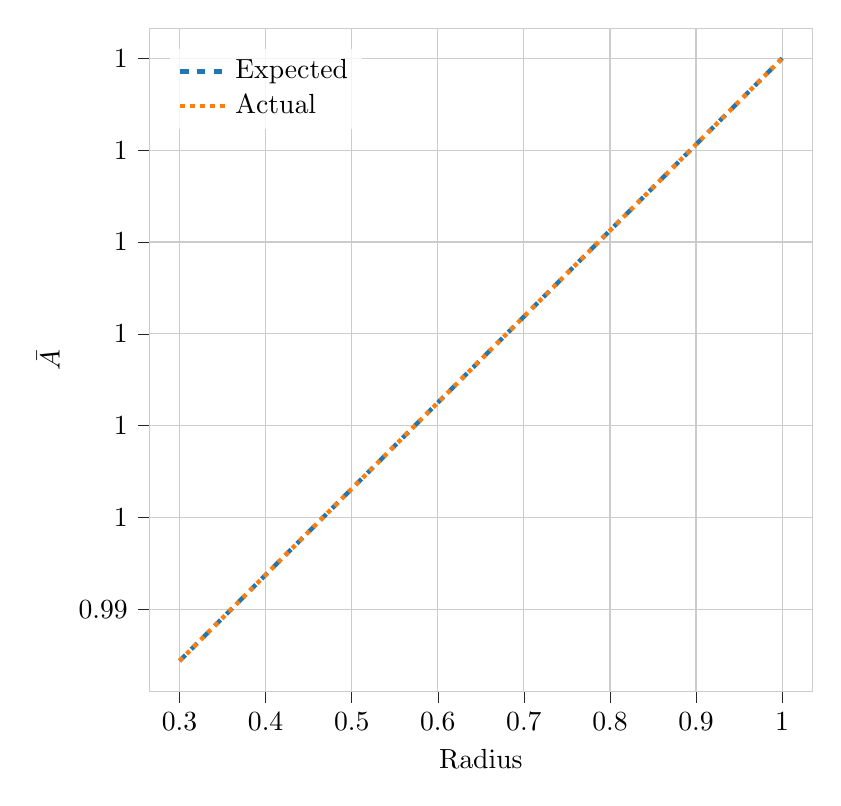
\begin{tikzpicture}

\definecolor{color0}{rgb}{0.12156862745098,0.466666666666667,0.705882352941177}
\definecolor{color1}{rgb}{1,0.498039215686275,0.0549019607843137}

\begin{axis}[
axis line style={white!80!black},
height=10cm,
legend cell align={left},
legend style={
  fill opacity=0.8,
  draw opacity=1,
  text opacity=1,
  at={(0.03,0.97)},
  anchor=north west,
  draw=none
},
tick align=outside,
tick pos=left,
width = 10cm,
x grid style={white!80!black},
xlabel={Radius},
xmajorgrids,
xmin=0.265, xmax=1.035,
xtick style={color=white!15!black},
y grid style={white!80!black},
ylabel={\(\displaystyle \bar{A}\)},
ymajorgrids,
ymin=0.993110580525858, ymax=1.00032806759401,
ytick style={color=white!15!black}
]
\addplot [ultra thick, color0, dashed]
table {%
0.3 0.993438648119864
0.30068093385214 0.993445029803663
0.30136186770428 0.993451411493035
0.30204280155642 0.993457793187971
0.30272373540856 0.993464174888459
0.3034046692607 0.993470556594488
0.30408560311284 0.993476938306049
0.304766536964981 0.993483320023129
0.305447470817121 0.993489701745718
0.306128404669261 0.993496083473805
0.306809338521401 0.99350246520738
0.307490272373541 0.99350884694643
0.308171206225681 0.993515228690947
0.308852140077821 0.993521610440918
0.309533073929961 0.993527992196332
0.310214007782101 0.99353437395718
0.310894941634241 0.99354075572345
0.311575875486381 0.993547137495131
0.312256809338521 0.993553519272212
0.312937743190661 0.993559901054684
0.313618677042802 0.993566282842533
0.314299610894942 0.99357266463575
0.314980544747082 0.993579046434325
0.315661478599222 0.993585428238245
0.316342412451362 0.993591810047501
0.317023346303502 0.993598191862081
0.317704280155642 0.993604573681974
0.318385214007782 0.99361095550717
0.319066147859922 0.993617337337658
0.319747081712062 0.993623719173427
0.320428015564202 0.993630101014466
0.321108949416342 0.993636482860764
0.321789883268483 0.99364286471231
0.322470817120623 0.993649246569094
0.323151750972763 0.993655628431104
0.323832684824903 0.99366201029833
0.324513618677043 0.993668392170761
0.325194552529183 0.993674774048386
0.325875486381323 0.993681155931194
0.326556420233463 0.993687537819175
0.327237354085603 0.993693919712317
0.327918287937743 0.993700301610609
0.328599221789883 0.993706683514042
0.329280155642023 0.993713065422603
0.329961089494163 0.993719447336282
0.330642023346304 0.993725829255068
0.331322957198444 0.993732211178951
0.332003891050584 0.993738593107918
0.332684824902724 0.993744975041961
0.333365758754864 0.993751356981067
0.334046692607004 0.993757738925226
0.334727626459144 0.993764120874427
0.335408560311284 0.99377050282866
0.336089494163424 0.993776884787912
0.336770428015564 0.993783266752174
0.337451361867704 0.993789648721434
0.338132295719844 0.993796030695682
0.338813229571985 0.993802412674907
0.339494163424124 0.993808794659097
0.340175097276265 0.993815176648243
0.340856031128405 0.993821558642333
0.341536964980545 0.993827940641357
0.342217898832685 0.993834322645302
0.342898832684825 0.99384070465416
0.343579766536965 0.993847086667918
0.344260700389105 0.993853468686566
0.344941634241245 0.993859850710094
0.345622568093385 0.993866232738489
0.346303501945525 0.993872614771742
0.346984435797665 0.993878996809841
0.347665369649805 0.993885378852776
0.348346303501946 0.993891760900536
0.349027237354086 0.99389814295311
0.349708171206226 0.993904525010486
0.350389105058366 0.993910907072655
0.351070038910506 0.993917289139605
0.351750972762646 0.993923671211325
0.352431906614786 0.993930053287805
0.353112840466926 0.993936435369034
0.353793774319066 0.993942817455
0.354474708171206 0.993949199545694
0.355155642023346 0.993955581641104
0.355836575875487 0.993961963741219
0.356517509727627 0.993968345846028
0.357198443579767 0.993974727955521
0.357879377431907 0.993981110069687
0.358560311284047 0.993987492188514
0.359241245136187 0.993993874311992
0.359922178988327 0.994000256440111
0.360603112840467 0.994006638572859
0.361284046692607 0.994013020710225
0.361964980544747 0.994019402852198
0.362645914396887 0.994025784998768
0.363326848249027 0.994032167149924
0.364007782101167 0.994038549305655
0.364688715953307 0.99404493146595
0.365369649805448 0.994051313630799
0.366050583657588 0.994057695800189
0.366731517509728 0.994064077974111
0.367412451361868 0.994070460152554
0.368093385214008 0.994076842335506
0.368774319066148 0.994083224522957
0.369455252918288 0.994089606714896
0.370136186770428 0.994095988911313
0.370817120622568 0.994102371112196
0.371498054474708 0.994108753317534
0.372178988326848 0.994115135527316
0.372859922178988 0.994121517741533
0.373540856031128 0.994127899960172
0.374221789883268 0.994134282183223
0.374902723735409 0.994140664410676
0.375583657587549 0.994147046642518
0.376264591439689 0.99415342887874
0.376945525291829 0.994159811119331
0.377626459143969 0.994166193364279
0.378307392996109 0.994172575613574
0.378988326848249 0.994178957867205
0.379669260700389 0.994185340125161
0.380350194552529 0.994191722387431
0.381031128404669 0.994198104654004
0.381712062256809 0.99420448692487
0.38239299610895 0.994210869200018
0.38307392996109 0.994217251479437
0.38375486381323 0.994223633763115
0.38443579766537 0.994230016051042
0.38511673151751 0.994236398343208
0.38579766536965 0.994242780639601
0.38647859922179 0.99424916294021
0.38715953307393 0.994255545245025
0.38784046692607 0.994261927554034
0.38852140077821 0.994268309867228
0.38920233463035 0.994274692184594
0.38988326848249 0.994281074506123
0.39056420233463 0.994287456831802
0.39124513618677 0.994293839161623
0.391926070038911 0.994300221495572
0.392607003891051 0.994306603833641
0.393287937743191 0.994312986175817
0.393968871595331 0.99431936852209
0.394649805447471 0.99432575087245
0.395330739299611 0.994332133226884
0.396011673151751 0.994338515585383
0.396692607003891 0.994344897947935
0.397373540856031 0.99435128031453
0.398054474708171 0.994357662685157
0.398735408560311 0.994364045059804
0.399416342412451 0.994370427438462
0.400097276264592 0.994376809821119
0.400778210116732 0.994383192207764
0.401459143968872 0.994389574598386
0.402140077821012 0.994395956992975
0.402821011673152 0.99440233939152
0.403501945525292 0.99440872179401
0.404182879377432 0.994415104200434
0.404863813229572 0.99442148661078
0.405544747081712 0.994427869025039
0.406225680933852 0.9944342514432
0.406906614785992 0.994440633865251
0.407587548638132 0.994447016291181
0.408268482490272 0.994453398720981
0.408949416342412 0.994459781154638
0.409630350194553 0.994466163592143
0.410311284046693 0.994472546033483
0.410992217898833 0.994478928478649
0.411673151750973 0.99448531092763
0.412354085603113 0.994491693380414
0.413035019455253 0.994498075836991
0.413715953307393 0.994504458297349
0.414396887159533 0.994510840761479
0.415077821011673 0.994517223229369
0.415758754863813 0.994523605701008
0.416439688715953 0.994529988176386
0.417120622568093 0.994536370655491
0.417801556420233 0.994542753138313
0.418482490272374 0.994549135624841
0.419163424124514 0.994555518115063
0.419844357976654 0.99456190060897
0.420525291828794 0.99456828310655
0.421206225680934 0.994574665607792
0.421887159533074 0.994581048112686
0.422568093385214 0.994587430621221
0.423249027237354 0.994593813133385
0.423929961089494 0.994600195649168
0.424610894941634 0.99460657816856
0.425291828793774 0.994612960691548
0.425972762645914 0.994619343218123
0.426653696498055 0.994625725748273
0.427334630350195 0.994632108281988
0.428015564202335 0.994638490819256
0.428696498054475 0.994644873360068
0.429377431906615 0.994651255904411
0.430058365758755 0.994657638452276
0.430739299610895 0.994664021003651
0.431420233463035 0.994670403558525
0.432101167315175 0.994676786116888
0.432782101167315 0.994683168678728
0.433463035019455 0.994689551244035
0.434143968871595 0.994695933812798
0.434824902723735 0.994702316385007
0.435505836575875 0.994708698960649
0.436186770428016 0.994715081539715
0.436867704280156 0.994721464122193
0.437548638132296 0.994727846708073
0.438229571984436 0.994734229297344
0.438910505836576 0.994740611889994
0.439591439688716 0.994746994486014
0.440272373540856 0.994753377085391
0.440953307392996 0.994759759688116
0.441634241245136 0.994766142294178
0.442315175097276 0.994772524903564
0.442996108949416 0.994778907516266
0.443677042801557 0.994785290132272
0.444357976653696 0.99479167275157
0.445038910505837 0.99479805537415
0.445719844357977 0.994804438000002
0.446400778210117 0.994810820629114
0.447081712062257 0.994817203261476
0.447762645914397 0.994823585897076
0.448443579766537 0.994829968535904
0.449124513618677 0.994836351177949
0.449805447470817 0.9948427338232
0.450486381322957 0.994849116471646
0.451167315175097 0.994855499123276
0.451848249027237 0.99486188177808
0.452529182879377 0.994868264436046
0.453210116731518 0.994874647097164
0.453891050583658 0.994881029761423
0.454571984435798 0.994887412428812
0.455252918287938 0.99489379509932
0.455933852140078 0.994900177772936
0.456614785992218 0.99490656044965
0.457295719844358 0.99491294312945
0.457976653696498 0.994919325812326
0.458657587548638 0.994925708498266
0.459338521400778 0.99493209118726
0.460019455252918 0.994938473879298
0.460700389105058 0.994944856574368
0.461381322957198 0.994951239272459
0.462062256809338 0.99495762197356
0.462743190661479 0.994964004677661
0.463424124513619 0.994970387384751
0.464105058365759 0.994976770094818
0.464785992217899 0.994983152807853
0.465466926070039 0.994989535523843
0.466147859922179 0.994995918242779
0.466828793774319 0.99500230096465
0.467509727626459 0.995008683689443
0.468190661478599 0.99501506641715
0.468871595330739 0.995021449147758
0.469552529182879 0.995027831881257
0.47023346303502 0.995034214617636
0.47091439688716 0.995040597356885
0.4715953307393 0.995046980098991
0.47227626459144 0.995053362843946
0.47295719844358 0.995059745591736
0.47363813229572 0.995066128342353
0.47431906614786 0.995072511095784
0.475 0.995078893852019
0.47568093385214 0.995085276611048
0.47636186770428 0.995091659372858
0.47704280155642 0.99509804213744
0.47772373540856 0.995104424904783
0.4784046692607 0.995110807674875
0.47908560311284 0.995117190447706
0.479766536964981 0.995123573223265
0.480447470817121 0.995129956001541
0.481128404669261 0.995136338782523
0.481809338521401 0.9951427215662
0.482490272373541 0.995149104352562
0.483171206225681 0.995155487141598
0.483852140077821 0.995161869933296
0.484533073929961 0.995168252727646
0.485214007782101 0.995174635524637
0.485894941634241 0.995181018324258
0.486575875486381 0.995187401126499
0.487256809338522 0.995193783931348
0.487937743190662 0.995200166738794
0.488618677042802 0.995206549548827
0.489299610894942 0.995212932361435
0.489980544747082 0.995219315176609
0.490661478599222 0.995225697994337
0.491342412451362 0.995232080814608
0.492023346303502 0.995238463637411
0.492704280155642 0.995244846462736
0.493385214007782 0.995251229290571
0.494066147859922 0.995257612120906
0.494747081712062 0.99526399495373
0.495428015564202 0.995270377789031
0.496108949416342 0.9952767606268
0.496789883268483 0.995283143467026
0.497470817120623 0.995289526309696
0.498151750972763 0.995295909154801
0.498832684824903 0.99530229200233
0.499513618677043 0.995308674852271
0.500194552529183 0.995315057704615
0.500875486381323 0.995321440559349
0.501556420233463 0.995327823416464
0.502237354085603 0.995334206275948
0.502918287937743 0.99534058913779
0.503599221789883 0.99534697200198
0.504280155642023 0.995353354868507
0.504961089494164 0.995359737737359
0.505642023346303 0.995366120608526
0.506322957198444 0.995372503481998
0.507003891050584 0.995378886357763
0.507684824902724 0.99538526923581
0.508365758754864 0.995391652116129
0.509046692607004 0.995398034998708
0.509727626459144 0.995404417883537
0.510408560311284 0.995410800770605
0.511089494163424 0.995417183659901
0.511770428015564 0.995423566551414
0.512451361867704 0.995429949445134
0.513132295719844 0.995436332341049
0.513813229571984 0.995442715239148
0.514494163424124 0.995449098139421
0.515175097276265 0.995455481041857
0.515856031128405 0.995461863946445
0.516536964980545 0.995468246853174
0.517217898832685 0.995474629762034
0.517898832684825 0.995481012673012
0.518579766536965 0.995487395586099
0.519260700389105 0.995493778501284
0.519941634241245 0.995500161418556
0.520622568093385 0.995506544337903
0.521303501945525 0.995512927259316
0.521984435797665 0.995519310182782
0.522665369649805 0.995525693108292
0.523346303501946 0.995532076035834
0.524027237354086 0.995538458965398
0.524708171206226 0.995544841896973
0.525389105058366 0.995551224830547
0.526070038910506 0.99555760776611
0.526750972762646 0.995563990703652
0.527431906614786 0.99557037364316
0.528112840466926 0.995576756584625
0.528793774319066 0.995583139528036
0.529474708171206 0.995589522473381
0.530155642023346 0.995595905420649
0.530836575875486 0.995602288369831
0.531517509727626 0.995608671320915
0.532198443579767 0.995615054273889
0.532879377431907 0.995621437228744
0.533560311284047 0.995627820185469
0.534241245136187 0.995634203144052
0.534922178988327 0.995640586104482
0.535603112840467 0.99564696906675
0.536284046692607 0.995653352030843
0.536964980544747 0.995659734996752
0.537645914396887 0.995666117964464
0.538326848249027 0.99567250093397
0.539007782101167 0.995678883905259
0.539688715953307 0.995685266878319
0.540369649805448 0.99569164985314
0.541050583657588 0.99569803282971
0.541731517509728 0.99570441580802
0.542412451361868 0.995710798788057
0.543093385214008 0.995717181769812
0.543774319066148 0.995723564753274
0.544455252918288 0.99572994773843
0.545136186770428 0.995736330725272
0.545817120622568 0.995742713713787
0.546498054474708 0.995749096703965
0.547178988326848 0.995755479695795
0.547859922178988 0.995761862689267
0.548540856031128 0.995768245684368
0.549221789883269 0.99577462868109
0.549902723735409 0.995781011679419
0.550583657587549 0.995787394679347
0.551264591439689 0.995793777680861
0.551945525291829 0.995800160683951
0.552626459143969 0.995806543688606
0.553307392996109 0.995812926694816
0.553988326848249 0.995819309702569
0.554669260700389 0.995825692711854
0.555350194552529 0.995832075722661
0.556031128404669 0.995838458734979
0.556712062256809 0.995844841748796
0.55739299610895 0.995851224764103
0.55807392996109 0.995857607780888
0.55875486381323 0.99586399079914
0.55943579766537 0.995870373818848
0.56011673151751 0.995876756840002
0.56079766536965 0.995883139862591
0.56147859922179 0.995889522886604
0.56215953307393 0.995895905912029
0.56284046692607 0.995902288938857
0.56352140077821 0.995908671967075
0.56420233463035 0.995915054996674
0.56488326848249 0.995921438027643
0.56556420233463 0.99592782105997
0.566245136186771 0.995934204093645
0.566926070038911 0.995940587128657
0.567607003891051 0.995946970164994
0.568287937743191 0.995953353202647
0.568968871595331 0.995959736241604
0.569649805447471 0.995966119281855
0.570330739299611 0.995972502323388
0.571011673151751 0.995978885366192
0.571692607003891 0.995985268410258
0.572373540856031 0.995991651455573
0.573054474708171 0.995998034502128
0.573735408560311 0.99600441754991
0.574416342412451 0.99601080059891
0.575097276264592 0.996017183649116
0.575778210116731 0.996023566700518
0.576459143968872 0.996029949753105
0.577140077821012 0.996036332806865
0.577821011673152 0.996042715861789
0.578501945525292 0.996049098917864
0.579182879377432 0.996055481975081
0.579863813229572 0.996061865033428
0.580544747081712 0.996068248092895
0.581225680933852 0.99607463115347
0.581906614785992 0.996081014215143
0.582587548638132 0.996087397277903
0.583268482490272 0.996093780341738
0.583949416342412 0.99610016340664
0.584630350194552 0.996106546472595
0.585311284046693 0.996112929539594
0.585992217898833 0.996119312607625
0.586673151750973 0.996125695676678
0.587354085603113 0.996132078746741
0.588035019455253 0.996138461817805
0.588715953307393 0.996144844889858
0.589396887159533 0.996151227962889
0.590077821011673 0.996157611036887
0.590758754863813 0.996163994111842
0.591439688715953 0.996170377187742
0.592120622568093 0.996176760264577
0.592801556420233 0.996183143342336
0.593482490272374 0.996189526421008
0.594163424124514 0.996195909500582
0.594844357976654 0.996202292581047
0.595525291828794 0.996208675662392
0.596206225680934 0.996215058744608
0.596887159533074 0.996221441827682
0.597568093385214 0.996227824911603
0.598249027237354 0.996234207996362
0.598929961089494 0.996240591081946
0.599610894941634 0.996246974168346
0.600291828793774 0.99625335725555
0.600972762645914 0.996259740343547
0.601653696498054 0.996266123432327
0.602334630350195 0.996272506521879
0.603015564202335 0.996278889612191
0.603696498054475 0.996285272703254
0.604377431906615 0.996291655795055
0.605058365758755 0.996298038887585
0.605739299610895 0.996304421980832
0.606420233463035 0.996310805074785
0.607101167315175 0.996317188169435
0.607782101167315 0.996323571264768
0.608463035019455 0.996329954360776
0.609143968871595 0.996336337457447
0.609824902723735 0.99634272055477
0.610505836575876 0.996349103652734
0.611186770428016 0.996355486751329
0.611867704280156 0.996361869850543
0.612548638132296 0.996368252950366
0.613229571984436 0.996374636050786
0.613910505836576 0.996381019151794
0.614591439688716 0.996387402253377
0.615272373540856 0.996393785355526
0.615953307392996 0.996400168458229
0.616634241245136 0.996406551561476
0.617315175097276 0.996412934665255
0.617996108949416 0.996419317769556
0.618677042801557 0.996425700874367
0.619357976653697 0.996432083979679
0.620038910505837 0.996438467085479
0.620719844357977 0.996444850191758
0.621400778210117 0.996451233298505
0.622081712062257 0.996457616405708
0.622762645914397 0.996463999513356
0.623443579766537 0.996470382621439
0.624124513618677 0.996476765729946
0.624805447470817 0.996483148838866
0.625486381322957 0.996489531948188
0.626167315175097 0.996495915057902
0.626848249027237 0.996502298167996
0.627529182879378 0.996508681278459
0.628210116731518 0.996515064389282
0.628891050583658 0.996521447500452
0.629571984435798 0.996527830611959
0.630252918287938 0.996534213723792
0.630933852140078 0.99654059683594
0.631614785992218 0.996546979948392
0.632295719844358 0.996553363061138
0.632976653696498 0.996559746174167
0.633657587548638 0.996566129287467
0.634338521400778 0.996572512401028
0.635019455252918 0.996578895514839
0.635700389105058 0.99658527862889
0.636381322957199 0.996591661743168
0.637062256809338 0.996598044857664
0.637743190661479 0.996604427972366
0.638424124513619 0.996610811087264
0.639105058365759 0.996617194202347
0.639785992217899 0.996623577317604
0.640466926070039 0.996629960433024
0.641147859922179 0.996636343548596
0.641828793774319 0.996642726664309
0.642509727626459 0.996649109780152
0.643190661478599 0.996655492896116
0.643871595330739 0.996661876012187
0.644552529182879 0.996668259128357
0.645233463035019 0.996674642244614
0.645914396887159 0.996681025360946
0.6465953307393 0.996687408477344
0.64727626459144 0.996693791593797
0.64795719844358 0.996700174710293
0.64863813229572 0.996706557826821
0.64931906614786 0.996712940943371
0.65 0.996719324059932
0.65068093385214 0.996725707176493
0.65136186770428 0.996732090293043
0.65204280155642 0.996738473409571
0.65272373540856 0.996744856526067
0.6534046692607 0.99675123964252
0.65408560311284 0.996757622758918
0.654766536964981 0.99676400587525
0.655447470817121 0.996770388991507
0.656128404669261 0.996776772107676
0.656809338521401 0.996783155223748
0.657490272373541 0.996789538339712
0.658171206225681 0.996795921455555
0.658852140077821 0.996802304571268
0.659533073929961 0.99680868768684
0.660214007782101 0.99681507080226
0.660894941634241 0.996821453917517
0.661575875486381 0.9968278370326
0.662256809338521 0.996834220147498
0.662937743190661 0.9968406032622
0.663618677042802 0.996846986376696
0.664299610894942 0.996853369490974
0.664980544747082 0.996859752605025
0.665661478599222 0.996866135718836
0.666342412451362 0.996872518832397
0.667023346303502 0.996878901945697
0.667704280155642 0.996885285058726
0.668385214007782 0.996891668171472
0.669066147859922 0.996898051283924
0.669747081712062 0.996904434396072
0.670428015564202 0.996910817507905
0.671108949416342 0.996917200619412
0.671789883268483 0.996923583730582
0.672470817120623 0.996929966841404
0.673151750972763 0.996936349951868
0.673832684824903 0.996942733061962
0.674513618677043 0.996949116171675
0.675194552529183 0.996955499280998
0.675875486381323 0.996961882389918
0.676556420233463 0.996968265498425
0.677237354085603 0.996974648606508
0.677918287937743 0.996981031714156
0.678599221789883 0.996987414821359
0.679280155642023 0.996993797928106
0.679961089494163 0.997000181034384
0.680642023346304 0.997006564140185
0.681322957198444 0.997012947245497
0.682003891050584 0.997019330350308
0.682684824902724 0.997025713454609
0.683365758754864 0.997032096558388
0.684046692607004 0.997038479661635
0.684727626459144 0.997044862764338
0.685408560311284 0.997051245866487
0.686089494163424 0.99705762896807
0.686770428015564 0.997064012069078
0.687451361867704 0.997070395169498
0.688132295719844 0.997076778269321
0.688813229571985 0.997083161368535
0.689494163424125 0.99708954446713
0.690175097276265 0.997095927565094
0.690856031128405 0.997102310662417
0.691536964980545 0.997108693759088
0.692217898832685 0.997115076855096
0.692898832684825 0.997121459950429
0.693579766536965 0.997127843045079
0.694260700389105 0.997134226139032
0.694941634241245 0.997140609232279
0.695622568093385 0.997146992324809
0.696303501945525 0.99715337541661
0.696984435797665 0.997159758507673
0.697665369649806 0.997166141597985
0.698346303501946 0.997172524687537
0.699027237354086 0.997178907776317
0.699708171206226 0.997185290864314
0.700389105058366 0.997191673951518
0.701070038910506 0.997198057037918
0.701750972762646 0.997204440123502
0.702431906614786 0.997210823208261
0.703112840466926 0.997217206292182
0.703793774319066 0.997223589375256
0.704474708171206 0.997229972457471
0.705155642023346 0.997236355538817
0.705836575875486 0.997242738619282
0.706517509727627 0.997249121698856
0.707198443579766 0.997255504777528
0.707879377431907 0.997261887855287
0.708560311284047 0.997268270932122
0.709241245136187 0.997274654008022
0.709922178988327 0.997281037082977
0.710603112840467 0.997287420156975
0.711284046692607 0.997293803230006
0.711964980544747 0.997300186302059
0.712645914396887 0.997306569373123
0.713326848249027 0.997312952443186
0.714007782101167 0.997319335512239
0.714688715953307 0.99732571858027
0.715369649805447 0.997332101647269
0.716050583657587 0.997338484713224
0.716731517509728 0.997344867778125
0.717412451361868 0.997351250841961
0.718093385214008 0.997357633904721
0.718774319066148 0.997364016966394
0.719455252918288 0.997370400026969
0.720136186770428 0.997376783086436
0.720817120622568 0.997383166144783
0.721498054474708 0.997389549202
0.722178988326848 0.997395932258075
0.722859922178988 0.997402315312999
0.723540856031128 0.997408698366759
0.724221789883268 0.997415081419346
0.724902723735409 0.997421464470748
0.725583657587549 0.997427847520954
0.726264591439689 0.997434230569954
0.726945525291829 0.997440613617736
0.727626459143969 0.997446996664291
0.728307392996109 0.997453379709606
0.728988326848249 0.997459762753672
0.729669260700389 0.997466145796476
0.730350194552529 0.997472528838009
0.731031128404669 0.99747891187826
0.73171206225681 0.997485294917217
0.732392996108949 0.99749167795487
0.73307392996109 0.997498060991207
0.73375486381323 0.997504444026219
0.73443579766537 0.997510827059894
0.73511673151751 0.997517210092221
0.73579766536965 0.99752359312319
0.73647859922179 0.997529976152789
0.73715953307393 0.997536359181007
0.73784046692607 0.997542742207835
0.73852140077821 0.99754912523326
0.73920233463035 0.997555508257273
0.73988326848249 0.997561891279862
0.74056420233463 0.997568274301016
0.74124513618677 0.997574657320724
0.741926070038911 0.997581040338976
0.742607003891051 0.997587423355761
0.743287937743191 0.997593806371068
0.743968871595331 0.997600189384885
0.744649805447471 0.997606572397203
0.745330739299611 0.99761295540801
0.746011673151751 0.997619338417295
0.746692607003891 0.997625721425048
0.747373540856031 0.997632104431258
0.748054474708171 0.997638487435913
0.748735408560311 0.997644870439003
0.749416342412451 0.997651253440517
0.750097276264592 0.997657636440445
0.750778210116732 0.997664019438774
0.751459143968872 0.997670402435496
0.752140077821012 0.997676785430597
0.752821011673152 0.997683168424068
0.753501945525292 0.997689551415899
0.754182879377432 0.997695934406077
0.754863813229572 0.997702317394592
0.755544747081712 0.997708700381434
0.756225680933852 0.99771508336659
0.756906614785992 0.997721466350052
0.757587548638132 0.997727849331807
0.758268482490272 0.997734232311844
0.758949416342413 0.997740615290154
0.759630350194553 0.997746998266724
0.760311284046693 0.997753381241545
0.760992217898833 0.997759764214605
0.761673151750973 0.997766147185894
0.762354085603113 0.9977725301554
0.763035019455253 0.997778913123112
0.763715953307393 0.997785296089021
0.764396887159533 0.997791679053114
0.765077821011673 0.997798062015381
0.765758754863813 0.997804444975812
0.766439688715953 0.997810827934395
0.767120622568093 0.99781721089112
0.767801556420234 0.997823593845975
0.768482490272373 0.997829976798949
0.769163424124514 0.997836359750033
0.769844357976654 0.997842742699214
0.770525291828794 0.997849125646483
0.771206225680934 0.997855508591828
0.771887159533074 0.997861891535239
0.772568093385214 0.997868274476704
0.773249027237354 0.997874657416212
0.773929961089494 0.997881040353754
0.774610894941634 0.997887423289317
0.775291828793774 0.997893806222891
0.775972762645914 0.997900189154466
0.776653696498054 0.99790657208403
0.777334630350194 0.997912955011572
0.778015564202335 0.997919337937082
0.778696498054475 0.997925720860548
0.779377431906615 0.997932103781961
0.780058365758755 0.997938486701308
0.780739299610895 0.99794486961858
0.781420233463035 0.997951252533765
0.782101167315175 0.997957635446852
0.782782101167315 0.99796401835783
0.783463035019455 0.99797040126669
0.784143968871595 0.997976784173419
0.784824902723735 0.997983167078007
0.785505836575875 0.997989549980443
0.786186770428016 0.997995932880716
0.786867704280156 0.998002315778815
0.787548638132296 0.99800869867473
0.788229571984436 0.99801508156845
0.788910505836576 0.998021464459963
0.789591439688716 0.998027847349259
0.790272373540856 0.998034230236327
0.790953307392996 0.998040613121156
0.791634241245136 0.998046996003735
0.792315175097276 0.998053378884054
0.792996108949416 0.998059761762101
0.793677042801556 0.998066144637866
0.794357976653696 0.998072527511338
0.795038910505837 0.998078910382505
0.795719844357977 0.998085293251357
0.796400778210117 0.998091676117884
0.797081712062257 0.998098058982074
0.797762645914397 0.998104441843916
0.798443579766537 0.9981108247034
0.799124513618677 0.998117207560515
0.799805447470817 0.998123590415249
0.800486381322957 0.998129973267593
0.801167315175097 0.998136356117534
0.801848249027237 0.998142738965063
0.802529182879377 0.998149121810168
0.803210116731518 0.998155504652838
0.803891050583658 0.998161887493064
0.804571984435798 0.998168270330832
0.805252918287938 0.998174653166134
0.805933852140078 0.998181035998958
0.806614785992218 0.998187418829293
0.807295719844358 0.998193801657128
0.807976653696498 0.998200184482453
0.808657587548638 0.998206567305256
0.809338521400778 0.998212950125527
0.810019455252918 0.998219332943255
0.810700389105058 0.998225715758428
0.811381322957198 0.998232098571037
0.812062256809339 0.99823848138107
0.812743190661479 0.998244864188516
0.813424124513619 0.998251246993365
0.814105058365759 0.998257629795606
0.814785992217899 0.998264012595227
0.815466926070039 0.998270395392218
0.816147859922179 0.998276778186568
0.816828793774319 0.998283160978266
0.817509727626459 0.998289543767302
0.818190661478599 0.998295926553664
0.818871595330739 0.998302309337341
0.819552529182879 0.998308692118323
0.82023346303502 0.998315074896599
0.82091439688716 0.998321457672158
0.8215953307393 0.998327840444989
0.82227626459144 0.998334223215081
0.82295719844358 0.998340605982424
0.82363813229572 0.998346988747006
0.82431906614786 0.998353371508816
0.825 0.998359754267845
0.82568093385214 0.99836613702408
0.82636186770428 0.998372519777511
0.82704280155642 0.998378902528128
0.82772373540856 0.998385285275918
0.828404669260701 0.998391668020873
0.829085603112841 0.998398050762979
0.829766536964981 0.998404433502228
0.830447470817121 0.998410816238607
0.831128404669261 0.998417198972106
0.831809338521401 0.998423581702714
0.832490272373541 0.998429964430421
0.833171206225681 0.998436347155214
0.833852140077821 0.998442729877085
0.834533073929961 0.998449112596021
0.835214007782101 0.998455495312011
0.835894941634241 0.998461878025046
0.836575875486381 0.998468260735113
0.837256809338522 0.998474643442203
0.837937743190662 0.998481026146304
0.838618677042802 0.998487408847405
0.839299610894942 0.998493791545496
0.839980544747082 0.998500174240566
0.840661478599222 0.998506556932603
0.841342412451362 0.998512939621598
0.842023346303502 0.998519322307538
0.842704280155642 0.998525704990414
0.843385214007782 0.998532087670214
0.844066147859922 0.998538470346928
0.844747081712062 0.998544853020544
0.845428015564202 0.998551235691052
0.846108949416343 0.998557618358441
0.846789883268482 0.9985640010227
0.847470817120623 0.998570383683818
0.848151750972763 0.998576766341784
0.848832684824903 0.998583148996588
0.849513618677043 0.998589531648218
0.850194552529183 0.998595914296664
0.850875486381323 0.998602296941915
0.851556420233463 0.99860867958396
0.852237354085603 0.998615062222788
0.852918287937743 0.998621444858388
0.853599221789883 0.99862782749075
0.854280155642023 0.998634210119862
0.854961089494163 0.998640592745714
0.855642023346303 0.998646975368294
0.856322957198444 0.998653357987592
0.857003891050584 0.998659740603598
0.857684824902724 0.9986661232163
0.858365758754864 0.998672505825686
0.859046692607004 0.998678888431748
0.859727626459144 0.998685271034473
0.860408560311284 0.99869165363385
0.861089494163424 0.99869803622987
0.861770428015564 0.99870441882252
0.862451361867704 0.998710801411791
0.863132295719844 0.998717183997671
0.863813229571984 0.998723566580149
0.864494163424125 0.998729949159215
0.865175097276265 0.998736331734857
0.865856031128405 0.998742714307066
0.866536964980545 0.998749096875829
0.867217898832685 0.998755479441136
0.867898832684825 0.998761862002976
0.868579766536965 0.998768244561339
0.869260700389105 0.998774627116213
0.869941634241245 0.998781009667588
0.870622568093385 0.998787392215453
0.871303501945525 0.998793774759796
0.871984435797665 0.998800157300607
0.872665369649805 0.998806539837876
0.873346303501946 0.998812922371591
0.874027237354086 0.998819304901741
0.874708171206226 0.998825687428316
0.875389105058366 0.998832069951304
0.876070038910506 0.998838452470696
0.876750972762646 0.998844834986479
0.877431906614786 0.998851217498643
0.878112840466926 0.998857600007178
0.878793774319066 0.998863982512072
0.879474708171206 0.998870365013314
0.880155642023346 0.998876747510894
0.880836575875486 0.998883130004801
0.881517509727627 0.998889512495023
0.882198443579767 0.998895894981551
0.882879377431907 0.998902277464373
0.883560311284047 0.998908659943478
0.884241245136187 0.998915042418856
0.884922178988327 0.998921424890495
0.885603112840467 0.998927807358385
0.886284046692607 0.998934189822514
0.886964980544747 0.998940572282873
0.887645914396887 0.99894695473945
0.888326848249027 0.998953337192234
0.889007782101167 0.998959719641215
0.889688715953307 0.998966102086381
0.890369649805448 0.998972484527721
0.891050583657588 0.998978866965226
0.891731517509728 0.998985249398883
0.892412451361868 0.998991631828682
0.893093385214008 0.998998014254613
0.893774319066148 0.999004396676664
0.894455252918288 0.999010779094825
0.895136186770428 0.999017161509084
0.895817120622568 0.99902354391943
0.896498054474708 0.999029926325854
0.897178988326848 0.999036308728344
0.897859922178988 0.999042691126888
0.898540856031128 0.999049073521478
0.899221789883269 0.9990554559121
0.899902723735409 0.999061838298745
0.900583657587549 0.999068220681402
0.901264591439689 0.99907460306006
0.901945525291829 0.999080985434707
0.902626459143969 0.999087367805334
0.903307392996109 0.999093750171929
0.903988326848249 0.999100132534481
0.904669260700389 0.99910651489298
0.905350194552529 0.999112897247414
0.906031128404669 0.999119279597774
0.906712062256809 0.999125661944047
0.90739299610895 0.999132044286223
0.90807392996109 0.999138426624292
0.90875486381323 0.999144808958241
0.90943579766537 0.999151191288062
0.91011673151751 0.999157573613741
0.91079766536965 0.99916395593527
0.91147859922179 0.999170338252636
0.91215953307393 0.99917672056583
0.91284046692607 0.999183102874839
0.91352140077821 0.999189485179654
0.91420233463035 0.999195867480263
0.91488326848249 0.999202249776656
0.91556420233463 0.999208632068822
0.91624513618677 0.999215014356749
0.91692607003891 0.999221396640427
0.917607003891051 0.999227778919846
0.918287937743191 0.999234161194994
0.918968871595331 0.99924054346586
0.919649805447471 0.999246925732433
0.920330739299611 0.999253307994703
0.921011673151751 0.999259690252659
0.921692607003891 0.99926607250629
0.922373540856031 0.999272454755585
0.923054474708171 0.999278837000533
0.923735408560311 0.999285219241124
0.924416342412451 0.999291601477346
0.925097276264591 0.999297983709188
0.925778210116732 0.999304365936641
0.926459143968872 0.999310748159692
0.927140077821012 0.999317130378331
0.927821011673152 0.999323512592548
0.928501945525292 0.99932989480233
0.929182879377432 0.999336277007668
0.929863813229572 0.999342659208551
0.930544747081712 0.999349041404968
0.931225680933852 0.999355423596907
0.931906614785992 0.999361805784358
0.932587548638132 0.99936818796731
0.933268482490272 0.999374570145753
0.933949416342412 0.999380952319675
0.934630350194552 0.999387334489065
0.935311284046693 0.999393716653914
0.935992217898833 0.999400098814208
0.936673151750973 0.999406480969939
0.937354085603113 0.999412863121095
0.938035019455253 0.999419245267666
0.938715953307393 0.999425627409639
0.939396887159533 0.999432009547005
0.940077821011673 0.999438391679753
0.940758754863813 0.999444773807872
0.941439688715953 0.99945115593135
0.942120622568093 0.999457538050177
0.942801556420233 0.999463920164343
0.943482490272374 0.999470302273836
0.944163424124514 0.999476684378645
0.944844357976654 0.99948306647876
0.945525291828794 0.99948944857417
0.946206225680934 0.999495830664863
0.946887159533074 0.99950221275083
0.947568093385214 0.999508594832059
0.948249027237354 0.999514976908539
0.948929961089494 0.999521358980259
0.949610894941634 0.999527741047209
0.950291828793774 0.999534123109378
0.950972762645914 0.999540505166754
0.951653696498054 0.999546887219328
0.952334630350194 0.999553269267088
0.953015564202334 0.999559651310022
0.953696498054475 0.999566033348122
0.954377431906615 0.999572415381375
0.955058365758755 0.99957879740977
0.955739299610895 0.999585179433298
0.956420233463035 0.999591561451946
0.957101167315175 0.999597943465704
0.957782101167315 0.999604325474562
0.958463035019455 0.999610707478507
0.959143968871595 0.999617089477531
0.959824902723735 0.999623471471621
0.960505836575875 0.999629853460767
0.961186770428015 0.999636235444957
0.961867704280156 0.999642617424182
0.962548638132296 0.99964899939843
0.963229571984436 0.99965538136769
0.963910505836576 0.999661763331952
0.964591439688716 0.999668145291204
0.965272373540856 0.999674527245437
0.965953307392996 0.999680909194638
0.966634241245136 0.999687291138797
0.967315175097276 0.999693673077903
0.967996108949416 0.999700055011945
0.968677042801556 0.999706436940913
0.969357976653697 0.999712818864796
0.970038910505837 0.999719200783582
0.970719844357977 0.999725582697261
0.971400778210117 0.999731964605822
0.972081712062257 0.999738346509255
0.972762645914397 0.999744728407547
0.973443579766537 0.999751110300689
0.974124513618677 0.99975749218867
0.974805447470817 0.999763874071478
0.975486381322957 0.999770255949103
0.976167315175097 0.999776637821534
0.976848249027237 0.99978301968876
0.977529182879378 0.99978940155077
0.978210116731518 0.999795783407554
0.978891050583658 0.9998021652591
0.979571984435798 0.999808547105398
0.980252918287938 0.999814928946437
0.980933852140078 0.999821310782206
0.981614785992218 0.999827692612694
0.982295719844358 0.99983407443789
0.982976653696498 0.999840456257783
0.983657587548638 0.999846838072363
0.984338521400778 0.999853219881619
0.985019455252918 0.999859601685539
0.985700389105058 0.999865983484113
0.986381322957199 0.999872365277331
0.987062256809339 0.99987874706518
0.987743190661479 0.999885128847651
0.988424124513619 0.999891510624733
0.989105058365759 0.999897892396414
0.989785992217899 0.999904274162684
0.990466926070039 0.999910655923532
0.991147859922179 0.999917037678946
0.991828793774319 0.999923419428917
0.992509727626459 0.999929801173434
0.993190661478599 0.999936182912484
0.993871595330739 0.999942564646059
0.99455252918288 0.999948946374146
0.99523346303502 0.999955328096735
0.99591439688716 0.999961709813815
0.9965953307393 0.999968091525376
0.99727626459144 0.999974473231405
0.99795719844358 0.999980854931893
0.99863813229572 0.999987236626829
0.99931906614786 0.999993618316201
1 1
};
\addlegendentry{Expected}
\addplot [ultra thick, color1, dotted]
table {%
0.3 0.993438648120748
0.30068093385214 0.993445029804545
0.30136186770428 0.993451411493917
0.30204280155642 0.993457793188852
0.30272373540856 0.993464174889339
0.3034046692607 0.993470556595368
0.30408560311284 0.993476938306927
0.304766536964981 0.993483320024006
0.305447470817121 0.993489701746594
0.306128404669261 0.993496083474681
0.306809338521401 0.993502465208254
0.307490272373541 0.993508846947304
0.308171206225681 0.99351522869182
0.308852140077821 0.99352161044179
0.309533073929961 0.993527992197204
0.310214007782101 0.993534373958051
0.310894941634241 0.99354075572432
0.311575875486381 0.993547137496
0.312256809338521 0.99355351927308
0.312937743190661 0.99355990105555
0.313618677042802 0.993566282843399
0.314299610894942 0.993572664636616
0.314980544747082 0.993579046435189
0.315661478599222 0.993585428239109
0.316342412451362 0.993591810048364
0.317023346303502 0.993598191862943
0.317704280155642 0.993604573682835
0.318385214007782 0.99361095550803
0.319066147859922 0.993617337338517
0.319747081712062 0.993623719174285
0.320428015564202 0.993630101015323
0.321108949416342 0.99363648286162
0.321789883268483 0.993642864713166
0.322470817120623 0.993649246569949
0.323151750972763 0.993655628431958
0.323832684824903 0.993662010299183
0.324513618677043 0.993668392171614
0.325194552529183 0.993674774049238
0.325875486381323 0.993681155932045
0.326556420233463 0.993687537820025
0.327237354085603 0.993693919713166
0.327918287937743 0.993700301611458
0.328599221789883 0.993706683514889
0.329280155642023 0.993713065423449
0.329961089494163 0.993719447337127
0.330642023346304 0.993725829255913
0.331322957198444 0.993732211179794
0.332003891050584 0.993738593108762
0.332684824902724 0.993744975042803
0.333365758754864 0.993751356981908
0.334046692607004 0.993757738926067
0.334727626459144 0.993764120875267
0.335408560311284 0.993770502829498
0.336089494163424 0.99377688478875
0.336770428015564 0.99378326675301
0.337451361867704 0.99378964872227
0.338132295719844 0.993796030696517
0.338813229571985 0.993802412675741
0.339494163424124 0.993808794659931
0.340175097276265 0.993815176649076
0.340856031128405 0.993821558643165
0.341536964980545 0.993827940642187
0.342217898832685 0.993834322646132
0.342898832684825 0.993840704654989
0.343579766536965 0.993847086668746
0.344260700389105 0.993853468687394
0.344941634241245 0.99385985071092
0.345622568093385 0.993866232739315
0.346303501945525 0.993872614772567
0.346984435797665 0.993878996810665
0.347665369649805 0.993885378853599
0.348346303501946 0.993891760901358
0.349027237354086 0.993898142953931
0.349708171206226 0.993904525011306
0.350389105058366 0.993910907073474
0.351070038910506 0.993917289140423
0.351750972762646 0.993923671212143
0.352431906614786 0.993930053288622
0.353112840466926 0.99393643536985
0.353793774319066 0.993942817455816
0.354474708171206 0.993949199546508
0.355155642023346 0.993955581641917
0.355836575875487 0.993961963742032
0.356517509727627 0.99396834584684
0.357198443579767 0.993974727956332
0.357879377431907 0.993981110070497
0.358560311284047 0.993987492189323
0.359241245136187 0.993993874312801
0.359922178988327 0.994000256440918
0.360603112840467 0.994006638573665
0.361284046692607 0.99401302071103
0.361964980544747 0.994019402853003
0.362645914396887 0.994025784999573
0.363326848249027 0.994032167150728
0.364007782101167 0.994038549306458
0.364688715953307 0.994044931466752
0.365369649805448 0.994051313631599
0.366050583657588 0.994057695800989
0.366731517509728 0.99406407797491
0.367412451361868 0.994070460153352
0.368093385214008 0.994076842336303
0.368774319066148 0.994083224523754
0.369455252918288 0.994089606715692
0.370136186770428 0.994095988912107
0.370817120622568 0.994102371112989
0.371498054474708 0.994108753318327
0.372178988326848 0.994115135528108
0.372859922178988 0.994121517742324
0.373540856031128 0.994127899960962
0.374221789883268 0.994134282184013
0.374902723735409 0.994140664411464
0.375583657587549 0.994147046643306
0.376264591439689 0.994153428879527
0.376945525291829 0.994159811120117
0.377626459143969 0.994166193365064
0.378307392996109 0.994172575614358
0.378988326848249 0.994178957867988
0.379669260700389 0.994185340125943
0.380350194552529 0.994191722388212
0.381031128404669 0.994198104654785
0.381712062256809 0.99420448692565
0.38239299610895 0.994210869200797
0.38307392996109 0.994217251480215
0.38375486381323 0.994223633763892
0.38443579766537 0.994230016051819
0.38511673151751 0.994236398343983
0.38579766536965 0.994242780640375
0.38647859922179 0.994249162940984
0.38715953307393 0.994255545245798
0.38784046692607 0.994261927554806
0.38852140077821 0.994268309867999
0.38920233463035 0.994274692185364
0.38988326848249 0.994281074506892
0.39056420233463 0.994287456832571
0.39124513618677 0.99429383916239
0.391926070038911 0.994300221496339
0.392607003891051 0.994306603834407
0.393287937743191 0.994312986176582
0.393968871595331 0.994319368522855
0.394649805447471 0.994325750873213
0.395330739299611 0.994332133227646
0.396011673151751 0.994338515586144
0.396692607003891 0.994344897948696
0.397373540856031 0.99435128031529
0.398054474708171 0.994357662685916
0.398735408560311 0.994364045060563
0.399416342412451 0.994370427439219
0.400097276264592 0.994376809821875
0.400778210116732 0.99438319220852
0.401459143968872 0.994389574599141
0.402140077821012 0.994395956993729
0.402821011673152 0.994402339392273
0.403501945525292 0.994408721794762
0.404182879377432 0.994415104201185
0.404863813229572 0.994421486611531
0.405544747081712 0.994427869025789
0.406225680933852 0.994434251443949
0.406906614785992 0.994440633865999
0.407587548638132 0.994447016291928
0.408268482490272 0.994453398721727
0.408949416342412 0.994459781155384
0.409630350194553 0.994466163592887
0.410311284046693 0.994472546034227
0.410992217898833 0.994478928479392
0.411673151750973 0.994485310928372
0.412354085603113 0.994491693381155
0.413035019455253 0.994498075837731
0.413715953307393 0.994504458298089
0.414396887159533 0.994510840762218
0.415077821011673 0.994517223230107
0.415758754863813 0.994523605701745
0.416439688715953 0.994529988177122
0.417120622568093 0.994536370656226
0.417801556420233 0.994542753139047
0.418482490272374 0.994549135625574
0.419163424124514 0.994555518115796
0.419844357976654 0.994561900609702
0.420525291828794 0.994568283107281
0.421206225680934 0.994574665608522
0.421887159533074 0.994581048113415
0.422568093385214 0.994587430621949
0.423249027237354 0.994593813134112
0.423929961089494 0.994600195649895
0.424610894941634 0.994606578169285
0.425291828793774 0.994612960692273
0.425972762645914 0.994619343218847
0.426653696498055 0.994625725748996
0.427334630350195 0.99463210828271
0.428015564202335 0.994638490819978
0.428696498054475 0.994644873360788
0.429377431906615 0.994651255905131
0.430058365758755 0.994657638452994
0.430739299610895 0.994664021004368
0.431420233463035 0.994670403559242
0.432101167315175 0.994676786117604
0.432782101167315 0.994683168679443
0.433463035019455 0.99468955124475
0.434143968871595 0.994695933813512
0.434824902723735 0.994702316385719
0.435505836575875 0.994708698961361
0.436186770428016 0.994715081540426
0.436867704280156 0.994721464122903
0.437548638132296 0.994727846708782
0.438229571984436 0.994734229298052
0.438910505836576 0.994740611890702
0.439591439688716 0.99474699448672
0.440272373540856 0.994753377086097
0.440953307392996 0.994759759688821
0.441634241245136 0.994766142294881
0.442315175097276 0.994772524904268
0.442996108949416 0.994778907516968
0.443677042801557 0.994785290132973
0.444357976653696 0.99479167275227
0.445038910505837 0.99479805537485
0.445719844357977 0.994804438000701
0.446400778210117 0.994810820629812
0.447081712062257 0.994817203262173
0.447762645914397 0.994823585897772
0.448443579766537 0.994829968536599
0.449124513618677 0.994836351178643
0.449805447470817 0.994842733823893
0.450486381322957 0.994849116472338
0.451167315175097 0.994855499123968
0.451848249027237 0.994861881778771
0.452529182879377 0.994868264436736
0.453210116731518 0.994874647097854
0.453891050583658 0.994881029762112
0.454571984435798 0.9948874124295
0.455252918287938 0.994893795100007
0.455933852140078 0.994900177773622
0.456614785992218 0.994906560450335
0.457295719844358 0.994912943130134
0.457976653696498 0.994919325813009
0.458657587548638 0.994925708498948
0.459338521400778 0.994932091187942
0.460019455252918 0.994938473879979
0.460700389105058 0.994944856575048
0.461381322957198 0.994951239273138
0.462062256809338 0.994957621974238
0.462743190661479 0.994964004678338
0.463424124513619 0.994970387385427
0.464105058365759 0.994976770095494
0.464785992217899 0.994983152808527
0.465466926070039 0.994989535524517
0.466147859922179 0.994995918243452
0.466828793774319 0.995002300965322
0.467509727626459 0.995008683690114
0.468190661478599 0.99501506641782
0.468871595330739 0.995021449148427
0.469552529182879 0.995027831881926
0.47023346303502 0.995034214618304
0.47091439688716 0.995040597357551
0.4715953307393 0.995046980099657
0.47227626459144 0.99505336284461
0.47295719844358 0.9950597455924
0.47363813229572 0.995066128343016
0.47431906614786 0.995072511096446
0.475 0.995078893852681
0.47568093385214 0.995085276611708
0.47636186770428 0.995091659373518
0.47704280155642 0.995098042138099
0.47772373540856 0.995104424905441
0.4784046692607 0.995110807675532
0.47908560311284 0.995117190448362
0.479766536964981 0.99512357322392
0.480447470817121 0.995129956002196
0.481128404669261 0.995136338783177
0.481809338521401 0.995142721566853
0.482490272373541 0.995149104353214
0.483171206225681 0.995155487142249
0.483852140077821 0.995161869933946
0.484533073929961 0.995168252728296
0.485214007782101 0.995174635525286
0.485894941634241 0.995181018324906
0.486575875486381 0.995187401127146
0.487256809338522 0.995193783931994
0.487937743190662 0.995200166739439
0.488618677042802 0.995206549549471
0.489299610894942 0.995212932362079
0.489980544747082 0.995219315177252
0.490661478599222 0.995225697994979
0.491342412451362 0.995232080815249
0.492023346303502 0.995238463638051
0.492704280155642 0.995244846463375
0.493385214007782 0.995251229291209
0.494066147859922 0.995257612121543
0.494747081712062 0.995263994954366
0.495428015564202 0.995270377789667
0.496108949416342 0.995276760627435
0.496789883268483 0.99528314346766
0.497470817120623 0.995289526310329
0.498151750972763 0.995295909155434
0.498832684824903 0.995302292002961
0.499513618677043 0.995308674852902
0.500194552529183 0.995315057705244
0.500875486381323 0.995321440559978
0.501556420233463 0.995327823417092
0.502237354085603 0.995334206276575
0.502918287937743 0.995340589138416
0.503599221789883 0.995346972002605
0.504280155642023 0.995353354869131
0.504961089494164 0.995359737737983
0.505642023346303 0.995366120609149
0.506322957198444 0.99537250348262
0.507003891050584 0.995378886358384
0.507684824902724 0.99538526923643
0.508365758754864 0.995391652116748
0.509046692607004 0.995398034999326
0.509727626459144 0.995404417884155
0.510408560311284 0.995410800771222
0.511089494163424 0.995417183660517
0.511770428015564 0.995423566552029
0.512451361867704 0.995429949445748
0.513132295719844 0.995436332341662
0.513813229571984 0.995442715239761
0.514494163424124 0.995449098140033
0.515175097276265 0.995455481042468
0.515856031128405 0.995461863947055
0.516536964980545 0.995468246853784
0.517217898832685 0.995474629762642
0.517898832684825 0.99548101267362
0.518579766536965 0.995487395586706
0.519260700389105 0.99549377850189
0.519941634241245 0.99550016141916
0.520622568093385 0.995506544338507
0.521303501945525 0.995512927259919
0.521984435797665 0.995519310183384
0.522665369649805 0.995525693108893
0.523346303501946 0.995532076036435
0.524027237354086 0.995538458965998
0.524708171206226 0.995544841897572
0.525389105058366 0.995551224831145
0.526070038910506 0.995557607766707
0.526750972762646 0.995563990704248
0.527431906614786 0.995570373643756
0.528112840466926 0.99557675658522
0.528793774319066 0.995583139528629
0.529474708171206 0.995589522473973
0.530155642023346 0.995595905421241
0.530836575875486 0.995602288370422
0.531517509727626 0.995608671321505
0.532198443579767 0.995615054274479
0.532879377431907 0.995621437229333
0.533560311284047 0.995627820186056
0.534241245136187 0.995634203144638
0.534922178988327 0.995640586105068
0.535603112840467 0.995646969067335
0.536284046692607 0.995653352031427
0.536964980544747 0.995659734997335
0.537645914396887 0.995666117965047
0.538326848249027 0.995672500934552
0.539007782101167 0.995678883905839
0.539688715953307 0.995685266878898
0.540369649805448 0.995691649853718
0.541050583657588 0.995698032830288
0.541731517509728 0.995704415808597
0.542412451361868 0.995710798788634
0.543093385214008 0.995717181770388
0.543774319066148 0.995723564753848
0.544455252918288 0.995729947739004
0.545136186770428 0.995736330725845
0.545817120622568 0.995742713714359
0.546498054474708 0.995749096704536
0.547178988326848 0.995755479696366
0.547859922178988 0.995761862689836
0.548540856031128 0.995768245684937
0.549221789883269 0.995774628681657
0.549902723735409 0.995781011679986
0.550583657587549 0.995787394679913
0.551264591439689 0.995793777681426
0.551945525291829 0.995800160684515
0.552626459143969 0.99580654368917
0.553307392996109 0.995812926695378
0.553988326848249 0.99581930970313
0.554669260700389 0.995825692712415
0.555350194552529 0.995832075723221
0.556031128404669 0.995838458735538
0.556712062256809 0.995844841749355
0.55739299610895 0.99585122476466
0.55807392996109 0.995857607781444
0.55875486381323 0.995863990799696
0.55943579766537 0.995870373819403
0.56011673151751 0.995876756840556
0.56079766536965 0.995883139863144
0.56147859922179 0.995889522887156
0.56215953307393 0.99589590591258
0.56284046692607 0.995902288939407
0.56352140077821 0.995908671967625
0.56420233463035 0.995915054997223
0.56488326848249 0.995921438028191
0.56556420233463 0.995927821060517
0.566245136186771 0.995934204094191
0.566926070038911 0.995940587129202
0.567607003891051 0.995946970165539
0.568287937743191 0.995953353203191
0.568968871595331 0.995959736242147
0.569649805447471 0.995966119282397
0.570330739299611 0.995972502323929
0.571011673151751 0.995978885366733
0.571692607003891 0.995985268410797
0.572373540856031 0.995991651456112
0.573054474708171 0.995998034502665
0.573735408560311 0.996004417550447
0.574416342412451 0.996010800599446
0.575097276264592 0.996017183649652
0.575778210116731 0.996023566701053
0.576459143968872 0.996029949753638
0.577140077821012 0.996036332807398
0.577821011673152 0.99604271586232
0.578501945525292 0.996049098918395
0.579182879377432 0.996055481975611
0.579863813229572 0.996061865033957
0.580544747081712 0.996068248093423
0.581225680933852 0.996074631153997
0.581906614785992 0.996081014215669
0.582587548638132 0.996087397278428
0.583268482490272 0.996093780342263
0.583949416342412 0.996100163407163
0.584630350194552 0.996106546473118
0.585311284046693 0.996112929540116
0.585992217898833 0.996119312608146
0.586673151750973 0.996125695677198
0.587354085603113 0.996132078747261
0.588035019455253 0.996138461818324
0.588715953307393 0.996144844890376
0.589396887159533 0.996151227963406
0.590077821011673 0.996157611037403
0.590758754863813 0.996163994112357
0.591439688715953 0.996170377188256
0.592120622568093 0.99617676026509
0.592801556420233 0.996183143342849
0.593482490272374 0.99618952642152
0.594163424124514 0.996195909501093
0.594844357976654 0.996202292581557
0.595525291828794 0.996208675662902
0.596206225680934 0.996215058745116
0.596887159533074 0.996221441828189
0.597568093385214 0.99622782491211
0.598249027237354 0.996234207996867
0.598929961089494 0.996240591082451
0.599610894941634 0.99624697416885
0.600291828793774 0.996253357256053
0.600972762645914 0.996259740344049
0.601653696498054 0.996266123432828
0.602334630350195 0.996272506522379
0.603015564202335 0.996278889612691
0.603696498054475 0.996285272703752
0.604377431906615 0.996291655795553
0.605058365758755 0.996298038888082
0.605739299610895 0.996304421981328
0.606420233463035 0.996310805075281
0.607101167315175 0.996317188169929
0.607782101167315 0.996323571265262
0.608463035019455 0.996329954361269
0.609143968871595 0.996336337457939
0.609824902723735 0.996342720555261
0.610505836575876 0.996349103653224
0.611186770428016 0.996355486751818
0.611867704280156 0.996361869851031
0.612548638132296 0.996368252950853
0.613229571984436 0.996374636051273
0.613910505836576 0.99638101915228
0.614591439688716 0.996387402253862
0.615272373540856 0.99639378535601
0.615953307392996 0.996400168458713
0.616634241245136 0.996406551561958
0.617315175097276 0.996412934665736
0.617996108949416 0.996419317770036
0.618677042801557 0.996425700874847
0.619357976653697 0.996432083980158
0.620038910505837 0.996438467085958
0.620719844357977 0.996444850192236
0.621400778210117 0.996451233298981
0.622081712062257 0.996457616406183
0.622762645914397 0.996463999513831
0.623443579766537 0.996470382621913
0.624124513618677 0.996476765730419
0.624805447470817 0.996483148839338
0.625486381322957 0.99648953194866
0.626167315175097 0.996495915058373
0.626848249027237 0.996502298168466
0.627529182879378 0.996508681278928
0.628210116731518 0.99651506438975
0.628891050583658 0.996521447500919
0.629571984435798 0.996527830612425
0.630252918287938 0.996534213724257
0.630933852140078 0.996540596836404
0.631614785992218 0.996546979948856
0.632295719844358 0.996553363061601
0.632976653696498 0.996559746174629
0.633657587548638 0.996566129287928
0.634338521400778 0.996572512401488
0.635019455252918 0.996578895515299
0.635700389105058 0.996585278629348
0.636381322957199 0.996591661743626
0.637062256809338 0.996598044858121
0.637743190661479 0.996604427972822
0.638424124513619 0.996610811087719
0.639105058365759 0.996617194202801
0.639785992217899 0.996623577318057
0.640466926070039 0.996629960433476
0.641147859922179 0.996636343549047
0.641828793774319 0.99664272666476
0.642509727626459 0.996649109780602
0.643190661478599 0.996655492896565
0.643871595330739 0.996661876012636
0.644552529182879 0.996668259128804
0.645233463035019 0.99667464224506
0.645914396887159 0.996681025361392
0.6465953307393 0.996687408477789
0.64727626459144 0.996693791594241
0.64795719844358 0.996700174710736
0.64863813229572 0.996706557827263
0.64931906614786 0.996712940943812
0.65 0.996719324060372
0.65068093385214 0.996725707176933
0.65136186770428 0.996732090293482
0.65204280155642 0.996738473410009
0.65272373540856 0.996744856526504
0.6534046692607 0.996751239642956
0.65408560311284 0.996757622759353
0.654766536964981 0.996764005875685
0.655447470817121 0.99677038899194
0.656128404669261 0.996776772108109
0.656809338521401 0.99678315522418
0.657490272373541 0.996789538340143
0.658171206225681 0.996795921455986
0.658852140077821 0.996802304571698
0.659533073929961 0.996808687687269
0.660214007782101 0.996815070802688
0.660894941634241 0.996821453917944
0.661575875486381 0.996827837033026
0.662256809338521 0.996834220147923
0.662937743190661 0.996840603262624
0.663618677042802 0.996846986377119
0.664299610894942 0.996853369491397
0.664980544747082 0.996859752605446
0.665661478599222 0.996866135719256
0.666342412451362 0.996872518832817
0.667023346303502 0.996878901946116
0.667704280155642 0.996885285059144
0.668385214007782 0.996891668171889
0.669066147859922 0.996898051284341
0.669747081712062 0.996904434396488
0.670428015564202 0.99691081750832
0.671108949416342 0.996917200619826
0.671789883268483 0.996923583730995
0.672470817120623 0.996929966841817
0.673151750972763 0.996936349952279
0.673832684824903 0.996942733062372
0.674513618677043 0.996949116172085
0.675194552529183 0.996955499281406
0.675875486381323 0.996961882390326
0.676556420233463 0.996968265498832
0.677237354085603 0.996974648606914
0.677918287937743 0.996981031714562
0.678599221789883 0.996987414821764
0.679280155642023 0.996993797928509
0.679961089494163 0.997000181034787
0.680642023346304 0.997006564140587
0.681322957198444 0.997012947245898
0.682003891050584 0.997019330350709
0.682684824902724 0.997025713455008
0.683365758754864 0.997032096558787
0.684046692607004 0.997038479662032
0.684727626459144 0.997044862764734
0.685408560311284 0.997051245866882
0.686089494163424 0.997057628968465
0.686770428015564 0.997064012069472
0.687451361867704 0.997070395169892
0.688132295719844 0.997076778269714
0.688813229571985 0.997083161368927
0.689494163424125 0.99708954446752
0.690175097276265 0.997095927565484
0.690856031128405 0.997102310662806
0.691536964980545 0.997108693759476
0.692217898832685 0.997115076855483
0.692898832684825 0.997121459950816
0.693579766536965 0.997127843045464
0.694260700389105 0.997134226139417
0.694941634241245 0.997140609232663
0.695622568093385 0.997146992325192
0.696303501945525 0.997153375416992
0.696984435797665 0.997159758508054
0.697665369649806 0.997166141598366
0.698346303501946 0.997172524687916
0.699027237354086 0.997178907776696
0.699708171206226 0.997185290864692
0.700389105058366 0.997191673951895
0.701070038910506 0.997198057038294
0.701750972762646 0.997204440123878
0.702431906614786 0.997210823208635
0.703112840466926 0.997217206292556
0.703793774319066 0.997223589375629
0.704474708171206 0.997229972457843
0.705155642023346 0.997236355539188
0.705836575875486 0.997242738619652
0.706517509727627 0.997249121699225
0.707198443579766 0.997255504777896
0.707879377431907 0.997261887855654
0.708560311284047 0.997268270932489
0.709241245136187 0.997274654008388
0.709922178988327 0.997281037083342
0.710603112840467 0.997287420157339
0.711284046692607 0.997293803230369
0.711964980544747 0.997300186302421
0.712645914396887 0.997306569373484
0.713326848249027 0.997312952443547
0.714007782101167 0.997319335512599
0.714688715953307 0.997325718580629
0.715369649805447 0.997332101647627
0.716050583657587 0.997338484713582
0.716731517509728 0.997344867778482
0.717412451361868 0.997351250842317
0.718093385214008 0.997357633905076
0.718774319066148 0.997364016966748
0.719455252918288 0.997370400027322
0.720136186770428 0.997376783086788
0.720817120622568 0.997383166145134
0.721498054474708 0.99738954920235
0.722178988326848 0.997395932258425
0.722859922178988 0.997402315313347
0.723540856031128 0.997408698367107
0.724221789883268 0.997415081419692
0.724902723735409 0.997421464471093
0.725583657587549 0.997427847521299
0.726264591439689 0.997434230570298
0.726945525291829 0.99744061361808
0.727626459143969 0.997446996664633
0.728307392996109 0.997453379709948
0.728988326848249 0.997459762754012
0.729669260700389 0.997466145796816
0.730350194552529 0.997472528838348
0.731031128404669 0.997478911878598
0.73171206225681 0.997485294917554
0.732392996108949 0.997491677955206
0.73307392996109 0.997498060991543
0.73375486381323 0.997504444026554
0.73443579766537 0.997510827060228
0.73511673151751 0.997517210092554
0.73579766536965 0.997523593123522
0.73647859922179 0.99752997615312
0.73715953307393 0.997536359181338
0.73784046692607 0.997542742208165
0.73852140077821 0.997549125233589
0.73920233463035 0.997555508257601
0.73988326848249 0.997561891280189
0.74056420233463 0.997568274301342
0.74124513618677 0.99757465732105
0.741926070038911 0.997581040339301
0.742607003891051 0.997587423356085
0.743287937743191 0.99759380637139
0.743968871595331 0.997600189385207
0.744649805447471 0.997606572397524
0.745330739299611 0.99761295540833
0.746011673151751 0.997619338417615
0.746692607003891 0.997625721425367
0.747373540856031 0.997632104431575
0.748054474708171 0.99763848743623
0.748735408560311 0.997644870439319
0.749416342412451 0.997651253440832
0.750097276264592 0.997657636440759
0.750778210116732 0.997664019439088
0.751459143968872 0.997670402435808
0.752140077821012 0.997676785430909
0.752821011673152 0.997683168424379
0.753501945525292 0.997689551416209
0.754182879377432 0.997695934406386
0.754863813229572 0.9977023173949
0.755544747081712 0.997708700381741
0.756225680933852 0.997715083366897
0.756906614785992 0.997721466350358
0.757587548638132 0.997727849332112
0.758268482490272 0.997734232312148
0.758949416342413 0.997740615290457
0.759630350194553 0.997746998267027
0.760311284046693 0.997753381241847
0.760992217898833 0.997759764214906
0.761673151750973 0.997766147186193
0.762354085603113 0.997772530155698
0.763035019455253 0.99777891312341
0.763715953307393 0.997785296089318
0.764396887159533 0.99779167905341
0.765077821011673 0.997798062015677
0.765758754863813 0.997804444976107
0.766439688715953 0.997810827934689
0.767120622568093 0.997817210891412
0.767801556420234 0.997823593846267
0.768482490272373 0.99782997679924
0.769163424124514 0.997836359750323
0.769844357976654 0.997842742699504
0.770525291828794 0.997849125646772
0.771206225680934 0.997855508592116
0.771887159533074 0.997861891535526
0.772568093385214 0.99786827447699
0.773249027237354 0.997874657416497
0.773929961089494 0.997881040354038
0.774610894941634 0.9978874232896
0.775291828793774 0.997893806223174
0.775972762645914 0.997900189154748
0.776653696498054 0.99790657208431
0.777334630350194 0.997912955011852
0.778015564202335 0.997919337937361
0.778696498054475 0.997925720860827
0.779377431906615 0.997932103782238
0.780058365758755 0.997938486701585
0.780739299610895 0.997944869618856
0.781420233463035 0.997951252534039
0.782101167315175 0.997957635447126
0.782782101167315 0.997964018358103
0.783463035019455 0.997970401266962
0.784143968871595 0.99797678417369
0.784824902723735 0.997983167078277
0.785505836575875 0.997989549980712
0.786186770428016 0.997995932880985
0.786867704280156 0.998002315779083
0.787548638132296 0.998008698674997
0.788229571984436 0.998015081568716
0.788910505836576 0.998021464460228
0.789591439688716 0.998027847349524
0.790272373540856 0.998034230236591
0.790953307392996 0.998040613121419
0.791634241245136 0.998046996003997
0.792315175097276 0.998053378884315
0.792996108949416 0.998059761762361
0.793677042801556 0.998066144638125
0.794357976653696 0.998072527511596
0.795038910505837 0.998078910382763
0.795719844357977 0.998085293251614
0.796400778210117 0.99809167611814
0.797081712062257 0.998098058982329
0.797762645914397 0.998104441844171
0.798443579766537 0.998110824703654
0.799124513618677 0.998117207560767
0.799805447470817 0.998123590415501
0.800486381322957 0.998129973267844
0.801167315175097 0.998136356117784
0.801848249027237 0.998142738965312
0.802529182879377 0.998149121810416
0.803210116731518 0.998155504653086
0.803891050583658 0.99816188749331
0.804571984435798 0.998168270331078
0.805252918287938 0.998174653166379
0.805933852140078 0.998181035999202
0.806614785992218 0.998187418829536
0.807295719844358 0.998193801657371
0.807976653696498 0.998200184482694
0.808657587548638 0.998206567305497
0.809338521400778 0.998212950125767
0.810019455252918 0.998219332943494
0.810700389105058 0.998225715758666
0.811381322957198 0.998232098571274
0.812062256809339 0.998238481381306
0.812743190661479 0.998244864188752
0.813424124513619 0.9982512469936
0.814105058365759 0.99825762979584
0.814785992217899 0.99826401259546
0.815466926070039 0.99827039539245
0.816147859922179 0.998276778186799
0.816828793774319 0.998283160978496
0.817509727626459 0.998289543767531
0.818190661478599 0.998295926553892
0.818871595330739 0.998302309337569
0.819552529182879 0.99830869211855
0.82023346303502 0.998315074896825
0.82091439688716 0.998321457672383
0.8215953307393 0.998327840445213
0.82227626459144 0.998334223215305
0.82295719844358 0.998340605982646
0.82363813229572 0.998346988747228
0.82431906614786 0.998353371509037
0.825 0.998359754268065
0.82568093385214 0.998366137024299
0.82636186770428 0.99837251977773
0.82704280155642 0.998378902528345
0.82772373540856 0.998385285276135
0.828404669260701 0.998391668021088
0.829085603112841 0.998398050763194
0.829766536964981 0.998404433502442
0.830447470817121 0.99841081623882
0.831128404669261 0.998417198972318
0.831809338521401 0.998423581702926
0.832490272373541 0.998429964430631
0.833171206225681 0.998436347155424
0.833852140077821 0.998442729877294
0.834533073929961 0.998449112596228
0.835214007782101 0.998455495312218
0.835894941634241 0.998461878025252
0.836575875486381 0.998468260735319
0.837256809338522 0.998474643442408
0.837937743190662 0.998481026146508
0.838618677042802 0.998487408847608
0.839299610894942 0.998493791545698
0.839980544747082 0.998500174240767
0.840661478599222 0.998506556932804
0.841342412451362 0.998512939621797
0.842023346303502 0.998519322307737
0.842704280155642 0.998525704990612
0.843385214007782 0.998532087670411
0.844066147859922 0.998538470347124
0.844747081712062 0.998544853020739
0.845428015564202 0.998551235691246
0.846108949416343 0.998557618358634
0.846789883268482 0.998564001022892
0.847470817120623 0.99857038368401
0.848151750972763 0.998576766341975
0.848832684824903 0.998583148996778
0.849513618677043 0.998589531648408
0.850194552529183 0.998595914296853
0.850875486381323 0.998602296942103
0.851556420233463 0.998608679584147
0.852237354085603 0.998615062222974
0.852918287937743 0.998621444858573
0.853599221789883 0.998627827490934
0.854280155642023 0.998634210120045
0.854961089494163 0.998640592745896
0.855642023346303 0.998646975368476
0.856322957198444 0.998653357987773
0.857003891050584 0.998659740603778
0.857684824902724 0.998666123216478
0.858365758754864 0.998672505825864
0.859046692607004 0.998678888431925
0.859727626459144 0.998685271034649
0.860408560311284 0.998691653634026
0.861089494163424 0.998698036230045
0.861770428015564 0.998704418822694
0.862451361867704 0.998710801411964
0.863132295719844 0.998717183997843
0.863813229571984 0.99872356658032
0.864494163424125 0.998729949159385
0.865175097276265 0.998736331735027
0.865856031128405 0.998742714307234
0.866536964980545 0.998749096875996
0.867217898832685 0.998755479441303
0.867898832684825 0.998761862003142
0.868579766536965 0.998768244561504
0.869260700389105 0.998774627116378
0.869941634241245 0.998781009667752
0.870622568093385 0.998787392215615
0.871303501945525 0.998793774759958
0.871984435797665 0.998800157300768
0.872665369649805 0.998806539838036
0.873346303501946 0.99881292237175
0.874027237354086 0.9988193049019
0.874708171206226 0.998825687428473
0.875389105058366 0.998832069951461
0.876070038910506 0.998838452470851
0.876750972762646 0.998844834986634
0.877431906614786 0.998851217498797
0.878112840466926 0.998857600007331
0.878793774319066 0.998863982512224
0.879474708171206 0.998870365013466
0.880155642023346 0.998876747511045
0.880836575875486 0.998883130004951
0.881517509727627 0.998889512495172
0.882198443579767 0.998895894981699
0.882879377431907 0.99890227746452
0.883560311284047 0.998908659943625
0.884241245136187 0.998915042419001
0.884922178988327 0.99892142489064
0.885603112840467 0.998927807358529
0.886284046692607 0.998934189822658
0.886964980544747 0.998940572283015
0.887645914396887 0.998946954739591
0.888326848249027 0.998953337192375
0.889007782101167 0.998959719641354
0.889688715953307 0.998966102086519
0.890369649805448 0.998972484527859
0.891050583657588 0.998978866965363
0.891731517509728 0.998985249399019
0.892412451361868 0.998991631828818
0.893093385214008 0.998998014254748
0.893774319066148 0.999004396676798
0.894455252918288 0.999010779094957
0.895136186770428 0.999017161509215
0.895817120622568 0.999023543919561
0.896498054474708 0.999029926325984
0.897178988326848 0.999036308728473
0.897859922178988 0.999042691127017
0.898540856031128 0.999049073521605
0.899221789883269 0.999055455912227
0.899902723735409 0.999061838298871
0.900583657587549 0.999068220681527
0.901264591439689 0.999074603060184
0.901945525291829 0.999080985434831
0.902626459143969 0.999087367805456
0.903307392996109 0.999093750172051
0.903988326848249 0.999100132534602
0.904669260700389 0.9991065148931
0.905350194552529 0.999112897247534
0.906031128404669 0.999119279597892
0.906712062256809 0.999125661944164
0.90739299610895 0.99913204428634
0.90807392996109 0.999138426624407
0.90875486381323 0.999144808958356
0.90943579766537 0.999151191288175
0.91011673151751 0.999157573613854
0.91079766536965 0.999163955935382
0.91147859922179 0.999170338252748
0.91215953307393 0.99917672056594
0.91284046692607 0.999183102874949
0.91352140077821 0.999189485179763
0.91420233463035 0.999195867480371
0.91488326848249 0.999202249776763
0.91556420233463 0.999208632068928
0.91624513618677 0.999215014356854
0.91692607003891 0.999221396640532
0.917607003891051 0.99922777891995
0.918287937743191 0.999234161195096
0.918968871595331 0.999240543465961
0.919649805447471 0.999246925732534
0.920330739299611 0.999253307994804
0.921011673151751 0.999259690252759
0.921692607003891 0.999266072506389
0.922373540856031 0.999272454755683
0.923054474708171 0.99927883700063
0.923735408560311 0.99928521924122
0.924416342412451 0.999291601477441
0.925097276264591 0.999297983709283
0.925778210116732 0.999304365936734
0.926459143968872 0.999310748159785
0.927140077821012 0.999317130378423
0.927821011673152 0.999323512592638
0.928501945525292 0.99932989480242
0.929182879377432 0.999336277007758
0.929863813229572 0.999342659208639
0.930544747081712 0.999349041405055
0.931225680933852 0.999355423596993
0.931906614785992 0.999361805784444
0.932587548638132 0.999368187967395
0.933268482490272 0.999374570145837
0.933949416342412 0.999380952319758
0.934630350194552 0.999387334489148
0.935311284046693 0.999393716653995
0.935992217898833 0.999400098814289
0.936673151750973 0.999406480970019
0.937354085603113 0.999412863121174
0.938035019455253 0.999419245267744
0.938715953307393 0.999425627409716
0.939396887159533 0.999432009547082
0.940077821011673 0.999438391679828
0.940758754863813 0.999444773807946
0.941439688715953 0.999451155931424
0.942120622568093 0.99945753805025
0.942801556420233 0.999463920164415
0.943482490272374 0.999470302273907
0.944163424124514 0.999476684378716
0.944844357976654 0.99948306647883
0.945525291828794 0.999489448574239
0.946206225680934 0.999495830664931
0.946887159533074 0.999502212750897
0.947568093385214 0.999508594832125
0.948249027237354 0.999514976908604
0.948929961089494 0.999521358980324
0.949610894941634 0.999527741047273
0.950291828793774 0.999534123109441
0.950972762645914 0.999540505166816
0.951653696498054 0.999546887219389
0.952334630350194 0.999553269267148
0.953015564202334 0.999559651310082
0.953696498054475 0.99956603334818
0.954377431906615 0.999572415381432
0.955058365758755 0.999578797409827
0.955739299610895 0.999585179433353
0.956420233463035 0.999591561452001
0.957101167315175 0.999597943465758
0.957782101167315 0.999604325474615
0.958463035019455 0.99961070747856
0.959143968871595 0.999617089477582
0.959824902723735 0.999623471471672
0.960505836575875 0.999629853460816
0.961186770428015 0.999636235445006
0.961867704280156 0.99964261742423
0.962548638132296 0.999648999398477
0.963229571984436 0.999655381367737
0.963910505836576 0.999661763331998
0.964591439688716 0.999668145291249
0.965272373540856 0.99967452724548
0.965953307392996 0.999680909194681
0.966634241245136 0.999687291138839
0.967315175097276 0.999693673077944
0.967996108949416 0.999700055011986
0.968677042801556 0.999706436940953
0.969357976653697 0.999712818864835
0.970038910505837 0.99971920078362
0.970719844357977 0.999725582697298
0.971400778210117 0.999731964605859
0.972081712062257 0.99973834650929
0.972762645914397 0.999744728407582
0.973443579766537 0.999751110300723
0.974124513618677 0.999757492188702
0.974805447470817 0.99976387407151
0.975486381322957 0.999770255949134
0.976167315175097 0.999776637821564
0.976848249027237 0.999783019688789
0.977529182879378 0.999789401550799
0.978210116731518 0.999795783407582
0.978891050583658 0.999802165259127
0.979571984435798 0.999808547105424
0.980252918287938 0.999814928946462
0.980933852140078 0.99982131078223
0.981614785992218 0.999827692612717
0.982295719844358 0.999834074437912
0.982976653696498 0.999840456257805
0.983657587548638 0.999846838072384
0.984338521400778 0.999853219881639
0.985019455252918 0.999859601685558
0.985700389105058 0.999865983484132
0.986381322957199 0.999872365277348
0.987062256809339 0.999878747065197
0.987743190661479 0.999885128847667
0.988424124513619 0.999891510624748
0.989105058365759 0.999897892396428
0.989785992217899 0.999904274162697
0.990466926070039 0.999910655923544
0.991147859922179 0.999917037678958
0.991828793774319 0.999923419428928
0.992509727626459 0.999929801173444
0.993190661478599 0.999936182912494
0.993871595330739 0.999942564646067
0.99455252918288 0.999948946374153
0.99523346303502 0.999955328096742
0.99591439688716 0.999961709813821
0.9965953307393 0.99996809152538
0.99727626459144 0.999974473231409
0.99795719844358 0.999980854931896
0.99863813229572 0.999987236626831
0.99931906614786 0.999993618316202
1 1
};
\addlegendentry{Actual}
\end{axis}

\end{tikzpicture}

%%    \newpage
%%    % This file was created with tikzplotlib v0.9.12.
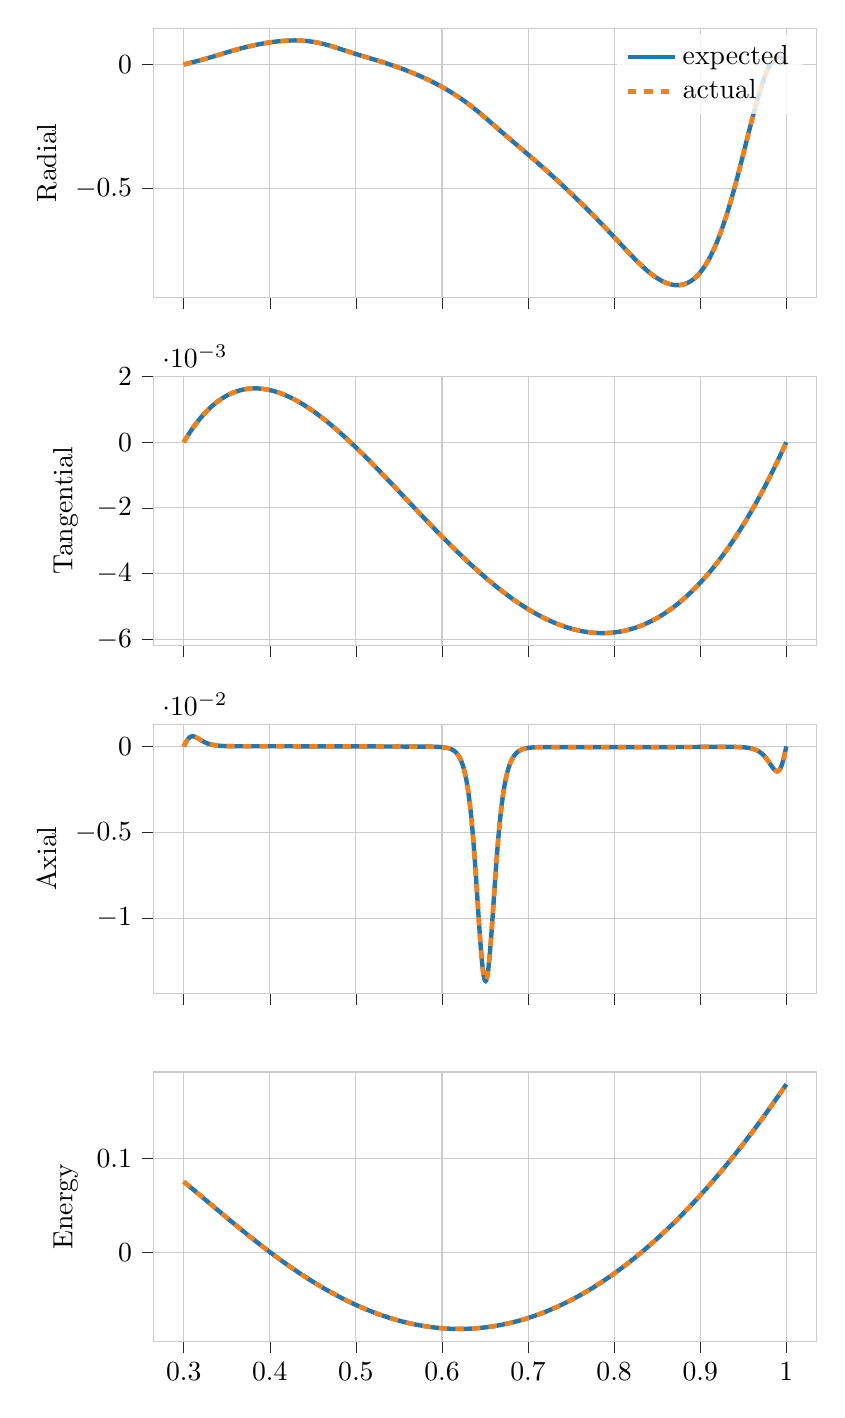
\begin{tikzpicture}

\definecolor{color0}{rgb}{0.12156862745098,0.466666666666667,0.705882352941177}
\definecolor{color1}{rgb}{1,0.498039215686275,0.0549019607843137}

\begin{groupplot}[group style={group size=1 by 4}]
\nextgroupplot[
axis line style={white!80!black},
height=5cm,
legend cell align={left},
legend style={fill opacity=0.8, draw opacity=1, text opacity=1, draw=none},
scaled x ticks=manual:{}{\pgfmathparse{#1}},
tick align=outside,
tick pos=left,
width=10cm,
x grid style={white!80!black},
xmajorgrids,
xmin=0.265, xmax=1.035,
xtick style={color=white!15!black},
xticklabels={},
y grid style={white!80!black},
ylabel={Radial},
ymajorgrids,
ymin=-0.939409659857244, ymax=0.146585062621206,
ytick style={color=white!15!black}
]
\addplot [ultra thick, color0]
table {%
0.3 -5.33253996515271e-15
0.30068093385214 0.000637683860963793
0.30136186770428 0.00127039902754333
0.30204280155642 0.00189863089008923
0.30272373540856 0.00252285970985274
0.3034046692607 0.00314355921961234
0.30408560311284 0.00376119526130104
0.304766536964981 0.00437622446905766
0.305447470817121 0.00498909300565832
0.306128404669261 0.00560023535974304
0.306809338521401 0.00621007321062755
0.307490272373541 0.00681901436680016
0.308171206225681 0.00742745178347828
0.308852140077821 0.00803576266380639
0.309533073929961 0.00864430764748903
0.310214007782101 0.00925343008980838
0.310894941634241 0.00986345543316011
0.311575875486381 0.0104746906724049
0.312256809338521 0.0110874239145316
0.312937743190661 0.0117019240323338
0.313618677042802 0.0123184404110559
0.314299610894942 0.0129372027862683
0.314980544747082 0.0135584211705445
0.315661478599222 0.014182285865946
0.316342412451362 0.0148089675587604
0.317023346303502 0.0154386174924544
0.317704280155642 0.0160713677144111
0.318385214007782 0.0167073313916618
0.319066147859922 0.0173466031905479
0.319747081712062 0.0179892597150399
0.320428015564202 0.0186353599982941
0.321108949416342 0.019284946041935
0.321789883268483 0.019938043397536
0.322470817120623 0.0205946617847838
0.323151750972763 0.0212547957409004
0.323832684824903 0.0219184252960151
0.324513618677043 0.0225855166693325
0.325194552529183 0.0232560229811553
0.325875486381323 0.0239298849760298
0.326556420233463 0.0246070317525477
0.327237354085603 0.0252873814956
0.327918287937743 0.025970842207167
0.328599221789883 0.0266573124320333
0.329280155642023 0.0273466819751037
0.329961089494163 0.0280388326073231
0.330642023346304 0.0287336387574871
0.331322957198444 0.0294309681875508
0.332003891050584 0.0301306826493279
0.332684824902724 0.0308326385207533
0.333365758754864 0.0315366874201762
0.334046692607004 0.0322426767973887
0.334727626459144 0.0329504505003627
0.335408560311284 0.0336598493168888
0.336089494163424 0.0343707114905372
0.336770428015564 0.0350828732105548
0.337451361867704 0.035796169075506
0.338132295719844 0.0365104325306199
0.338813229571985 0.0372254962789786
0.339494163424124 0.037941192666799
0.340175097276265 0.0386573540431966
0.340856031128405 0.0393738130949182
0.341536964980545 0.0400904031566211
0.342217898832685 0.0408069584973688
0.342898832684825 0.0415233145840676
0.343579766536965 0.0422393083226187
0.344260700389105 0.0429547782776293
0.344941634241245 0.0436695648715306
0.345622568093385 0.0443835105639954
0.346303501945525 0.0450964600125569
0.346984435797665 0.0458082602153409
0.347665369649805 0.0465187606368287
0.348346303501946 0.0472278133175537
0.349027237354086 0.0479352729686478
0.349708171206226 0.048640997052112
0.350389105058366 0.049344845847692
0.351070038910506 0.0500466825072034
0.351750972762646 0.050746373097138
0.352431906614786 0.0514437866303499
0.353112840466926 0.0521387950875928
0.353793774319066 0.0528312734296516
0.354474708171206 0.0535210996007864
0.355155642023346 0.0542081545241622
0.355836575875487 0.0548923220899206
0.356517509727627 0.0555734891365066
0.357198443579767 0.0562515454258434
0.357879377431907 0.056926383612895
0.358560311284047 0.0575978992101602
0.359241245136187 0.058265990547569
0.359922178988327 0.0589305587282597
0.360603112840467 0.0595915075806569
0.361284046692607 0.0602487436072674
0.361964980544747 0.0609021759305583
0.362645914396887 0.0615517162362786
0.363326848249027 0.0621972787145407
0.364007782101167 0.0628387799989731
0.364688715953307 0.0634761391042071
0.365369649805448 0.0641092773619716
0.366050583657588 0.064738118356013
0.366731517509728 0.0653625878560678
0.367412451361868 0.0659826137510732
0.368093385214008 0.0665981259818061
0.368774319066148 0.0672090564730953
0.369455252918288 0.0678153390657687
0.370136186770428 0.0684169094484502
0.370817120622568 0.069013705089338
0.371498054474708 0.0696056651680542
0.372178988326848 0.0701927305076622
0.372859922178988 0.0707748435069359
0.373540856031128 0.0713519480729395
0.374221789883268 0.0719239895539865
0.374902723735409 0.0724909146730247
0.375583657587549 0.0730526714614852
0.376264591439689 0.0736092091936338
0.376945525291829 0.0741604783214526
0.377626459143969 0.0747064304100634
0.378307392996109 0.0752470180737191
0.378988326848249 0.0757821949123583
0.379669260700389 0.0763119154487379
0.380350194552529 0.0768361350661372
0.381031128404669 0.077354809946624
0.381712062256809 0.0778678970098858
0.38239299610895 0.0783753538525973
0.38307392996109 0.0788771386883273
0.38375486381323 0.0793732102879481
0.38443579766537 0.0798635279205442
0.38511673151751 0.080348051294786
0.38579766536965 0.0808267405007516
0.38647859922179 0.0812995559521712
0.38715953307393 0.0817664583290618
0.38784046692607 0.0822274085207362
0.38852140077821 0.0826823675691505
0.38920233463035 0.0831312966125648
0.38988326848249 0.0835741568294937
0.39056420233463 0.0840109093829135
0.39124513618677 0.0844415153647065
0.391926070038911 0.0848659357403101
0.392607003891051 0.0852841312935515
0.393287937743191 0.0856960625716436
0.393968871595331 0.08610168983032
0.394649805447471 0.0865009729790872
0.395330739299611 0.0868938715265867
0.396011673151751 0.0872803445260372
0.396692607003891 0.0876603505207561
0.397373540856031 0.0880338474897519
0.398054474708171 0.0884007927933691
0.398735408560311 0.0887611431190053
0.399416342412451 0.089114854426875
0.400097276264592 0.0894618818958593
0.400778210116732 0.0898021798694205
0.401459143968872 0.0901357018016263
0.402140077821012 0.0904624002032822
0.402821011673152 0.0907822265882243
0.403501945525292 0.0910951314197839
0.404182879377432 0.0914010640574869
0.404863813229572 0.091699972704019
0.405544747081712 0.0919918043525335
0.406225680933852 0.0922765047343503
0.406906614785992 0.0925540182671305
0.407587548638132 0.0928242880036147
0.408268482490272 0.0930872555810142
0.408949416342412 0.0933428611711595
0.409630350194553 0.0935910434315384
0.410311284046693 0.0938317394573359
0.410992217898833 0.0940648847346345
0.411673151750973 0.0942904130949234
0.412354085603113 0.09450825667109
0.413035019455253 0.0947183458550919
0.413715953307393 0.0949206092574876
0.414396887159533 0.0951149736690734
0.415077821011673 0.0953013640248478
0.415758754863813 0.0954797033705575
0.416439688715953 0.0956499128321091
0.417120622568093 0.0958119115881303
0.417801556420233 0.0959656168459978
0.418482490272374 0.0961109438216664
0.419163424124514 0.0962478057236529
0.419844357976654 0.0963761137415527
0.420525291828794 0.0964957770394843
0.421206225680934 0.0966067027548846
0.421887159533074 0.0967087960031003
0.422568093385214 0.0968019598882338
0.423249027237354 0.0968860955207346
0.423929961089494 0.0969611020422426
0.424610894941634 0.0970268766582145
0.425291828793774 0.0970833146788787
0.425972762645914 0.0971303095690926
0.426653696498055 0.0971677530076792
0.427334630350195 0.0971955349568561
0.428015564202335 0.0972135437423622
0.428696498054475 0.0972216661449131
0.429377431906615 0.097219787503624
0.430058365758755 0.097207791832032
0.430739299610895 0.0971855619473735
0.431420233463035 0.0971529796137369
0.432101167315175 0.0971099256997448
0.432782101167315 0.0970562803513682
0.433463035019455 0.096991923180479
0.434143968871595 0.0969167334697183
0.434824902723735 0.0968305903942201
0.435505836575875 0.0967333732606948
0.436186770428016 0.0966249617643261
0.436867704280156 0.0965052362638829
0.437548638132296 0.096374078075372
0.438229571984436 0.0962313697844884
0.438910505836576 0.096076995578032
0.439591439688716 0.0959108415943563
0.440272373540856 0.0957327962928146
0.440953307392996 0.095542750842033
0.441634241245136 0.0953405995267285
0.442315175097276 0.0951262401726197
0.442996108949416 0.0948995745888466
0.443677042801557 0.0946605090271256
0.444357976653696 0.0944089546567093
0.445038910505837 0.094144828053999
0.445719844357977 0.093868051705502
0.446400778210117 0.0935785545225744
0.447081712062257 0.0932762723661989
0.447762645914397 0.092961148579831
0.448443579766537 0.0926331345280951
0.449124513618677 0.0922921901389188
0.449805447470817 0.0919382844464384
0.450486381322957 0.0915713961318073
0.451167315175097 0.091191514058813
0.451848249027237 0.0907986378009999
0.452529182879377 0.090392778156806
0.453210116731518 0.0899739576490419
0.453891050583658 0.089542211004885
0.454571984435798 0.0890975856124231
0.455252918287938 0.0886401419496826
0.455933852140078 0.088169953981998
0.456614785992218 0.0876871095235431
0.457295719844358 0.0871917105588397
0.457976653696498 0.0866838735201121
0.458657587548638 0.0861637295164326
0.459338521400778 0.0856314245107368
0.460019455252918 0.085087119440994
0.460700389105058 0.0845309902820132
0.461381322957198 0.083963228044694
0.462062256809338 0.0833840387098397
0.462743190661479 0.0827936430940488
0.463424124513619 0.0821922766456403
0.464105058365759 0.0815801891690413
0.464785992217899 0.0809576444765971
0.465466926070039 0.0803249199673186
0.466147859922179 0.0796823061326754
0.466828793774319 0.0790301059901654
0.467509727626459 0.0783686344460177
0.468190661478599 0.0776982175890418
0.468871595330739 0.0770191919182739
0.469552529182879 0.0763319035077198
0.47023346303502 0.0756367071121135
0.47091439688716 0.0749339652182123
0.4715953307393 0.0742240470467167
0.47227626459144 0.0735073275104174
0.47295719844358 0.0727841861346593
0.47363813229572 0.0720550059466097
0.47431906614786 0.0713201723401726
0.475 0.0705800719236714
0.47568093385214 0.0698350913576131
0.47636186770428 0.0690856161899759
0.47704280155642 0.0683320296965007
0.47772373540856 0.067574711733419
0.4784046692607 0.0668140376099305
0.47908560311284 0.066050376987543
0.479766536964981 0.0652840928130874
0.480447470817121 0.064515540291898
0.481128404669261 0.0637450659072011
0.481809338521401 0.0629730064912906
0.482490272373541 0.0621996883535396
0.483171206225681 0.0614254264697081
0.483852140077821 0.0606505237364247
0.484533073929961 0.0598752702940464
0.485214007782101 0.0590999429204921
0.485894941634241 0.0583248044979483
0.486575875486381 0.0575501035537055
0.487256809338522 0.0567760738757448
0.487937743190662 0.0560029342030407
0.488618677042802 0.0552308879899572
0.489299610894942 0.0544601232435537
0.489980544747082 0.0536908124320505
0.490661478599222 0.0529231124622461
0.491342412451362 0.0521571647232215
0.492023346303502 0.051393095193263
0.492704280155642 0.0506310146066107
0.493385214007782 0.0498710186763397
0.494066147859922 0.0491131883694419
0.494747081712062 0.0483575902300041
0.495428015564202 0.0476042767462328
0.496108949416342 0.0468532867570051
0.496789883268483 0.0461046458935756
0.497470817120623 0.0453583670520888
0.498151750972763 0.0446144508925888
0.498832684824903 0.0438728863602966
0.499513618677043 0.0431336512250531
0.500194552529183 0.0423967126349693
0.500875486381323 0.0416620276804847
0.501556420233463 0.0409295439652481
0.502237354085603 0.0401992001804106
0.502918287937743 0.0394709266791855
0.503599221789883 0.0387446460487172
0.504280155642023 0.0380202736765685
0.504961089494164 0.0372977183093555
0.505642023346303 0.0365768826013214
0.506322957198444 0.0358576636508544
0.507003891050584 0.0351399535232057
0.507684824902724 0.03442363975788
0.508365758754864 0.0337086058594045
0.509046692607004 0.0329947317703687
0.509727626459144 0.0322818943258495
0.510408560311284 0.0315699676885078
0.511089494163424 0.0308588237638241
0.511770428015564 0.0301483325951065
0.512451361867704 0.0294383627380447
0.513132295719844 0.0287287816147306
0.513813229571984 0.028019455847187
0.514494163424124 0.0273102515705547
0.515175097276265 0.0266010347261944
0.515856031128405 0.0258916713350446
0.516536964980545 0.0251820277516507
0.517217898832685 0.0244719708993561
0.517898832684825 0.0237613684871903
0.518579766536965 0.0230500892090474
0.519260700389105 0.0223380029257764
0.519941634241245 0.0216249808308501
0.520622568093385 0.0209108956002764
0.521303501945525 0.0201956215274613
0.521984435797665 0.019479034643724
0.522665369649805 0.0187610128251694
0.523346303501946 0.0180414358866374
0.524027237354086 0.0173201856634199
0.524708171206226 0.0165971460814557
0.525389105058366 0.0158722032166713
0.526070038910506 0.0151452453441502
0.526750972762646 0.0144161629777744
0.527431906614786 0.0136848489009684
0.528112840466926 0.0129511981891653
0.528793774319066 0.0122151082245741
0.529474708171206 0.0114764787038213
0.530155642023346 0.0107352116390053
0.530836575875486 0.00999121135268204
0.531517509727626 0.00924438446727052
0.532198443579767 0.00849463988935823
0.532879377431907 0.00774188878933057
0.533560311284047 0.0069860445767639
0.534241245136187 0.00622702287196299
0.534922178988327 0.00546474147401739
0.535603112840467 0.00469912032573249
0.536284046692607 0.00393008147574955
0.536964980544747 0.00315754903816945
0.537645914396887 0.00238144914995963
0.538326848249027 0.00160170992640763
0.539007782101167 0.00081826141486489
0.539688715953307 3.10355470105397e-05
0.540369649805448 -0.000760033910159802
0.541050583657588 -0.00155501140442814
0.541731517509728 -0.00235395964935459
0.542412451361868 -0.00315693967602508
0.543093385214008 -0.0039640108853975
0.543774319066148 -0.00477523110111806
0.544455252918288 -0.00559065662268294
0.545136186770428 -0.00641034227883782
0.545817120622568 -0.00723434148112623
0.546498054474708 -0.00806270627748838
0.547178988326848 -0.00889548740584266
0.547859922178988 -0.00973273434758145
0.548540856031128 -0.0105744953809184
0.549221789883269 -0.0114208176340452
0.549902723735409 -0.0122717471380438
0.550583657587549 -0.0131273288795265
0.551264591439689 -0.0139876068529736
0.551945525291829 -0.0148526241127389
0.552626459143969 -0.0157224228247069
0.553307392996109 -0.0165970443175967
0.553988326848249 -0.0174765291338887
0.554669260700389 -0.0183609170803826
0.555350194552529 -0.0192502472783783
0.556031128404669 -0.0201445582134831
0.556712062256809 -0.0210438877850556
0.55739299610895 -0.0219482733552877
0.55807392996109 -0.0228577517979437
0.55875486381323 -0.0237723595467584
0.55943579766537 -0.0246921326435218
0.56011673151751 -0.0256171067858586
0.56079766536965 -0.0265473173747197
0.56147859922179 -0.027482799561618
0.56215953307393 -0.0284235882956038
0.56284046692607 -0.029369718370027
0.56352140077821 -0.0303212244690937
0.56420233463035 -0.031278141214232
0.56488326848249 -0.0322405032103083
0.56556420233463 -0.0332083450916943
0.566245136186771 -0.0341817015682201
0.566926070038911 -0.0351606074710253
0.567607003891051 -0.0361450977983304
0.568287937743191 -0.0371352077611476
0.568968871595331 -0.0381309728289447
0.569649805447471 -0.0391324287752795
0.570330739299611 -0.0401396117234179
0.571011673151751 -0.0411525581919463
0.571692607003891 -0.0421713051403905
0.572373540856031 -0.0431958900148409
0.573054474708171 -0.0442263507935968
0.573735408560311 -0.0452627260328229
0.574416342412451 -0.0463050549122204
0.575097276264592 -0.0473533772807019
0.575778210116731 -0.0484077337020668
0.576459143968872 -0.0494681655006523
0.577140077821012 -0.0505347148069496
0.577821011673152 -0.0516074246031575
0.578501945525292 -0.0526863387686382
0.579182879377432 -0.0537715021252507
0.579863813229572 -0.0548629604825098
0.580544747081712 -0.0559607606825221
0.581225680933852 -0.0570649506446471
0.581906614785992 -0.0581755794098189
0.582587548638132 -0.0592926971844516
0.583268482490272 -0.0604163553838498
0.583949416342412 -0.0615466066750332
0.584630350194552 -0.0626835050188782
0.585311284046693 -0.063827105711456
0.585992217898833 -0.0649774654244579
0.586673151750973 -0.0661346422445595
0.587354085603113 -0.067298695711594
0.588035019455253 -0.0684696868553577
0.588715953307393 -0.0696476782308876
0.589396887159533 -0.0708327339520201
0.590077821011673 -0.0720249197230279
0.590758754863813 -0.0732243028681157
0.591439688715953 -0.0744309523585473
0.592120622568093 -0.0756449388371466
0.592801556420233 -0.0768663346399092
0.593482490272374 -0.0780952138144399
0.594163424124514 -0.079331652134909
0.594844357976654 -0.0805757271132063
0.595525291828794 -0.0818275180059582
0.596206225680934 -0.0830871058170362
0.596887159533074 -0.0843545732951874
0.597568093385214 -0.0856300049263856
0.598249027237354 -0.0869134869204818
0.598929961089494 -0.0882051071917245
0.599610894941634 -0.0895049553326895
0.600291828793774 -0.0908131225811475
0.600972762645914 -0.0921297017793863
0.601653696498054 -0.0934547873254734
0.602334630350195 -0.094788475115948
0.603015564202335 -0.0961308624794108
0.603696498054475 -0.0974820481004624
0.604377431906615 -0.098842131933449
0.605058365758755 -0.10021121510546
0.605739299610895 -0.101589399808011
0.606420233463035 -0.102976789176867
0.607101167315175 -0.104373487159458
0.607782101167315 -0.105779598369323
0.608463035019455 -0.1071952279271
0.609143968871595 -0.108620481287509
0.609824902723735 -0.110055464051884
0.610505836575876 -0.111500281765804
0.611186770428016 -0.112955039701401
0.611867704280156 -0.114419842624002
0.612548638132296 -0.115894794542812
0.613229571984436 -0.117379998445376
0.613910505836576 -0.118875556015678
0.614591439688716 -0.120381567335793
0.615272373540856 -0.121898130571096
0.615953307392996 -0.12342534163915
0.616634241245136 -0.124963293862496
0.617315175097276 -0.126512077605707
0.617996108949416 -0.128071779897165
0.618677042801557 -0.129642484036224
0.619357976653697 -0.131224269186506
0.620038910505837 -0.132817209956292
0.620719844357977 -0.13442137596711
0.621400778210117 -0.136036831411832
0.622081712062257 -0.137663634603719
0.622762645914397 -0.139301837518125
0.623443579766537 -0.14095148532868
0.624124513618677 -0.14261261594003
0.624805447470817 -0.144285259519386
0.625486381322957 -0.145969438029302
0.626167315175097 -0.147665164764338
0.626848249027237 -0.149372443894407
0.627529182879378 -0.151091270017774
0.628210116731518 -0.152821627726869
0.628891050583658 -0.154563491190159
0.629571984435798 -0.156316823753491
0.630252918287938 -0.158081577564379
0.630933852140078 -0.159857693222806
0.631614785992218 -0.161645099462113
0.632295719844358 -0.163443712863598
0.632976653696498 -0.165253437608373
0.633657587548638 -0.167074165269995
0.634338521400778 -0.168905774651245
0.635019455252918 -0.170748131668306
0.635700389105058 -0.172601089285375
0.636381322957199 -0.174464487502515
0.637062256809338 -0.176338153399268
0.637743190661479 -0.178221901236214
0.638424124513619 -0.180115532616314
0.639105058365759 -0.182018836707434
0.639785992217899 -0.183931590527044
0.640466926070039 -0.185853559289562
0.641147859922179 -0.187784496816359
0.641828793774319 -0.189724146007866
0.642509727626459 -0.191672239376709
0.643190661478599 -0.193628499640255
0.643871595330739 -0.195592640370345
0.644552529182879 -0.197564366697513
0.645233463035019 -0.199543376066388
0.645914396887159 -0.201529359038488
0.6465953307393 -0.203522000138125
0.64727626459144 -0.205520978736694
0.64795719844358 -0.207525969970166
0.64863813229572 -0.209536645684311
0.64931906614786 -0.211552675401813
0.65 -0.213573727305223
0.65068093385214 -0.215599469229504
0.65136186770428 -0.217629569657822
0.65204280155642 -0.219663698714178
0.65272373540856 -0.221701529146504
0.6534046692607 -0.223742737293958
0.65408560311284 -0.225787004032307
0.654766536964981 -0.227834015691516
0.655447470817121 -0.229883464939951
0.656128404669261 -0.231935051629988
0.656809338521401 -0.233988483600165
0.657490272373541 -0.236043477429508
0.658171206225681 -0.23809975914014
0.658852140077821 -0.240157064844775
0.659533073929961 -0.242215141336271
0.660214007782101 -0.244273746616941
0.660894941634241 -0.24633265036591
0.661575875486381 -0.248391634343356
0.662256809338521 -0.250450492731015
0.662937743190661 -0.252509032408899
0.663618677042802 -0.254567073168659
0.664299610894942 -0.256624447864557
0.664980544747082 -0.258681002503435
0.665661478599222 -0.260736596275501
0.666342412451362 -0.262791101528168
0.667023346303502 -0.264844403685474
0.667704280155642 -0.266896401115943
0.668385214007782 -0.268947004951998
0.669066147859922 -0.270996138864232
0.669747081712062 -0.273043738794008
0.670428015564202 -0.275089752648
0.671108949416342 -0.277134139958323
0.671789883268483 -0.279176871511993
0.672470817120623 -0.281217928953386
0.673151750972763 -0.283257304363409
0.673832684824903 -0.285294999818958
0.674513618677043 -0.287331026936201
0.675194552529183 -0.289365406401044
0.675875486381323 -0.29139816749007
0.676556420233463 -0.293429347584993
0.677237354085603 -0.295458991683589
0.677918287937743 -0.297487151909791
0.678599221789883 -0.299513887025501
0.679280155642023 -0.301539261946454
0.679961089494163 -0.303563347264253
0.680642023346304 -0.305586218776501
0.681322957198444 -0.307607957026754
0.682003891050584 -0.309628646855823
0.682684824902724 -0.311648376965749
0.683365758754864 -0.313667239497588
0.684046692607004 -0.315685329623983
0.684727626459144 -0.317702745157309
0.685408560311284 -0.319719586174019
0.686089494163424 -0.321735954655681
0.686770428015564 -0.323751954147038
0.687451361867704 -0.325767689431326
0.688132295719844 -0.327783266222905
0.688813229571985 -0.329798790877235
0.689494163424125 -0.33181437011805
0.690175097276265 -0.333830110781559
0.690856031128405 -0.335846119577383
0.691536964980545 -0.337862502865894
0.692217898832685 -0.339879366451565
0.692898832684825 -0.341896815391863
0.693579766536965 -0.34391495382122
0.694260700389105 -0.345933884789539
0.694941634241245 -0.347953710114694
0.695622568093385 -0.349974530248446
0.696303501945525 -0.351996444155207
0.696984435797665 -0.354019549203028
0.697665369649806 -0.356043941066237
0.698346303501946 -0.358069713639111
0.699027237354086 -0.360096958959999
0.699708171206226 -0.362125767145281
0.700389105058366 -0.364156226332615
0.701070038910506 -0.366188422632876
0.701750972762646 -0.368222440090241
0.702431906614786 -0.370258360649888
0.703112840466926 -0.372296264132772
0.703793774319066 -0.374336228216994
0.704474708171206 -0.376378328425261
0.705155642023346 -0.378422638117982
0.705836575875486 -0.380469228491555
0.706517509727627 -0.382518168581426
0.707198443579766 -0.384569525269506
0.707879377431907 -0.386623363295583
0.708560311284047 -0.388679745272349
0.709241245136187 -0.390738731703719
0.709922178988327 -0.392800381006109
0.710603112840467 -0.394864749532375
0.711284046692607 -0.39693189159814
0.711964980544747 -0.399001859510228
0.712645914396887 -0.401074703596979
0.713326848249027 -0.403150472240197
0.714007782101167 -0.405229211908534
0.714688715953307 -0.407310967192105
0.715369649805447 -0.409395780838151
0.716050583657587 -0.41148369378759
0.716731517509728 -0.413574745212295
0.717412451361868 -0.415668972552961
0.718093385214008 -0.417766411557432
0.718774319066148 -0.41986709631937
0.719455252918288 -0.421971059317165
0.720136186770428 -0.424078331452973
0.720817120622568 -0.426188942091825
0.721498054474708 -0.428302919100697
0.722178988326848 -0.430420288887498
0.722859922178988 -0.432541076439898
0.723540856031128 -0.434665305363951
0.724221789883268 -0.436792997922463
0.724902723735409 -0.438924175073069
0.725583657587549 -0.441058856505978
0.726264591439689 -0.443197060681357
0.726945525291829 -0.445338804866338
0.727626459143969 -0.447484105171624
0.728307392996109 -0.449632976587673
0.728988326848249 -0.451785433020463
0.729669260700389 -0.45394148732681
0.730350194552529 -0.456101151349262
0.731031128404669 -0.45826443595054
0.73171206225681 -0.460431351047546
0.732392996108949 -0.462601905644933
0.73307392996109 -0.464776107868247
0.73375486381323 -0.46695396499665
0.73443579766537 -0.46913548349522
0.73511673151751 -0.471320669046865
0.73579766536965 -0.473509526583834
0.73647859922179 -0.475702060318859
0.73715953307393 -0.477898273775927
0.73784046692607 -0.480098169820714
0.73852140077821 -0.482301750690668
0.73920233463035 -0.484509018024789
0.73988326848249 -0.486719972893096
0.74056420233463 -0.4889346158258
0.74124513618677 -0.491152946842207
0.741926070038911 -0.493374965479354
0.742607003891051 -0.495600670820398
0.743287937743191 -0.49783006152276
0.743968871595331 -0.500063135846045
0.744649805447471 -0.502299891679744
0.745330739299611 -0.504540326570716
0.746011673151751 -0.506784437750478
0.746692607003891 -0.509032222162274
0.747373540856031 -0.511283676487962
0.748054474708171 -0.51353879717468
0.748735408560311 -0.51579758046132
0.749416342412451 -0.518060022404781
0.750097276264592 -0.520326118906
0.750778210116732 -0.522595865735747
0.751459143968872 -0.52486925856016
0.752140077821012 -0.527146292966011
0.752821011673152 -0.529426964485658
0.753501945525292 -0.531711268621669
0.754182879377432 -0.53399920087107
0.754863813229572 -0.536290756749181
0.755544747081712 -0.538585931812987
0.756225680933852 -0.540884721683992
0.756906614785992 -0.543187122070492
0.757587548638132 -0.545493128789198
0.758268482490272 -0.547802737786137
0.758949416342413 -0.550115945156738
0.759630350194553 -0.552432747165008
0.760311284046693 -0.554753140261709
0.760992217898833 -0.557077121101396
0.761673151750973 -0.559404686558221
0.762354085603113 -0.561735833740351
0.763035019455253 -0.564070560002848
0.763715953307393 -0.566408862958872
0.764396887159533 -0.568750740489015
0.765077821011673 -0.571096190748599
0.765758754863813 -0.573445212172717
0.766439688715953 -0.575797803478836
0.767120622568093 -0.578153963666692
0.767801556420234 -0.580513692015279
0.768482490272373 -0.582876988076631
0.769163424124514 -0.585243851666158
0.769844357976654 -0.587614282849209
0.770525291828794 -0.589988281923585
0.771206225680934 -0.592365849397649
0.771887159533074 -0.594746985963712
0.772568093385214 -0.59713169246631
0.773249027237354 -0.599519969865021
0.773929961089494 -0.601911819191403
0.774610894941634 -0.604307241499656
0.775291828793774 -0.606706237810576
0.775972762645914 -0.609108809048361
0.776653696498054 -0.611514955969801
0.777334630350194 -0.613924679085401
0.778015564202335 -0.616337978571948
0.778696498054475 -0.618754854176015
0.779377431906615 -0.621175305107935
0.780058365758755 -0.623599329925714
0.780739299610895 -0.626026926408396
0.781420233463035 -0.628458091418355
0.782101167315175 -0.630892820752044
0.782782101167315 -0.633331108978672
0.783463035019455 -0.635772949266358
0.784143968871595 -0.63821833319529
0.784824902723735 -0.640667250557449
0.785505836575875 -0.64311968914249
0.786186770428016 -0.645575634509401
0.786867704280156 -0.648035069743616
0.787548638132296 -0.650497975199293
0.788229571984436 -0.652964328226523
0.788910505836576 -0.655434102883319
0.789591439688716 -0.657907269632287
0.790272373540856 -0.660383795021975
0.790953307392996 -0.662863641352979
0.791634241245136 -0.66534676632899
0.792315175097276 -0.667833122693077
0.792996108949416 -0.670322657849608
0.793677042801556 -0.672815313472345
0.794357976653696 -0.675311025099401
0.795038910505837 -0.677809721715844
0.795719844357977 -0.680311325324949
0.796400778210117 -0.682815750509199
0.797081712062257 -0.685322903982334
0.797762645914397 -0.687832684133918
0.798443579766537 -0.690344980568024
0.799124513618677 -0.692859673637888
0.799805447470817 -0.695376633978469
0.800486381322957 -0.697895722039093
0.801167315175097 -0.700416787618499
0.801848249027237 -0.702939669404753
0.802529182879377 -0.70546419452268
0.803210116731518 -0.707990178091584
0.803891050583658 -0.710517422796147
0.804571984435798 -0.713045718473519
0.805252918287938 -0.7155748417197
0.805933852140078 -0.718104555518353
0.806614785992218 -0.720634608895263
0.807295719844358 -0.723164736601625
0.807976653696498 -0.725694658829356
0.808657587548638 -0.728224080961539
0.809338521400778 -0.730752693361027
0.810019455252918 -0.733280171200113
0.810700389105058 -0.735806174333982
0.811381322957198 -0.738330347220449
0.812062256809339 -0.740852318888285
0.812743190661479 -0.743371702956076
0.813424124513619 -0.745888097703292
0.814105058365759 -0.748401086194855
0.814785992217899 -0.750910236460119
0.815466926070039 -0.753415101726731
0.816147859922179 -0.755915220709434
0.816828793774319 -0.758410117953359
0.817509727626459 -0.760899304230914
0.818190661478599 -0.763382276990866
0.818871595330739 -0.765858520857716
0.819552529182879 -0.76832750817899
0.82023346303502 -0.770788699617601
0.82091439688716 -0.773241544785926
0.8215953307393 -0.775685482917882
0.82227626459144 -0.778119943574809
0.82295719844358 -0.780544347380656
0.82363813229572 -0.782958106781597
0.82431906614786 -0.785360626824972
0.825 -0.787751305952195
0.82568093385214 -0.790129536800123
0.82636186770428 -0.792494707005268
0.82704280155642 -0.794846200005207
0.82772373540856 -0.797183395831543
0.828404669260701 -0.799505671888863
0.829085603112841 -0.801812403714305
0.829766536964981 -0.804102965712497
0.830447470817121 -0.806376731860942
0.831128404669261 -0.808633076381207
0.831809338521401 -0.810871374371614
0.832490272373541 -0.813091002397576
0.833171206225681 -0.81529133903609
0.833852140077821 -0.817471765371406
0.834533073929961 -0.819631665439356
0.835214007782101 -0.821770426618294
0.835894941634241 -0.82388743996516
0.836575875486381 -0.825982100495604
0.837256809338522 -0.828053807407681
0.837937743190662 -0.830101964249025
0.838618677042802 -0.832125979027973
0.839299610894942 -0.834125264269452
0.839980544747082 -0.836099237016928
0.840661478599222 -0.838047318782059
0.841342412451362 -0.839968935444051
0.842023346303502 -0.84186351710105
0.842704280155642 -0.843730497876112
0.843385214007782 -0.845569315680598
0.844066147859922 -0.847379411937988
0.844747081712062 -0.849160231271266
0.845428015564202 -0.850911221157151
0.846108949416343 -0.852631831550521
0.846789883268482 -0.854321514482414
0.847470817120623 -0.855979723634996
0.848151750972763 -0.857605913896878
0.848832684824903 -0.859199540902082
0.849513618677043 -0.860760060555916
0.850194552529183 -0.86228692855088
0.850875486381323 -0.86377959987565
0.851556420233463 -0.86523752832
0.852237354085603 -0.866660165978438
0.852918287937743 -0.868046962755102
0.853599221789883 -0.86939736587237
0.854280155642023 -0.87071081938541
0.854961089494163 -0.871986763704737
0.855642023346303 -0.873224635128716
0.856322957198444 -0.874423865387692
0.857003891050584 -0.875583881201345
0.857684824902724 -0.876704103850636
0.858365758754864 -0.877783948765608
0.859046692607004 -0.878822825130098
0.859727626459144 -0.879820135504342
0.860408560311284 -0.880775275466228
0.861089494163424 -0.88168763327193
0.861770428015564 -0.882556589536456
0.862451361867704 -0.883381516934575
0.863132295719844 -0.884161779922495
0.863813229571984 -0.884896734480558
0.864494163424125 -0.885585727877143
0.865175097276265 -0.886228098453931
0.865856031128405 -0.886823175432564
0.866536964980545 -0.887370278742751
0.867217898832685 -0.887868718871783
0.867898832684825 -0.888317796735388
0.868579766536965 -0.888716803569868
0.869260700389105 -0.88906502084538
0.869941634241245 -0.889361720200269
0.870622568093385 -0.889606163396301
0.871303501945525 -0.88979760229468
0.871984435797665 -0.889935278852709
0.872665369649805 -0.890018425140978
0.873346303501946 -0.890046263380951
0.874027237354086 -0.890018006002872
0.874708171206226 -0.889932855723877
0.875389105058366 -0.889790005646277
0.876070038910506 -0.889588639375933
0.876750972762646 -0.889327931160735
0.877431906614786 -0.889007046049153
0.878112840466926 -0.888625140068917
0.878793774319066 -0.888181360425862
0.879474708171206 -0.887674845723031
0.880155642023346 -0.887104726200133
0.880836575875486 -0.886470123993516
0.881517509727627 -0.885770153416786
0.882198443579767 -0.885003921262315
0.882879377431907 -0.88417052712381
0.883560311284047 -0.883269063740227
0.884241245136187 -0.882298617361291
0.884922178988327 -0.88125826813493
0.885603112840467 -0.880147090516943
0.886284046692607 -0.878964153703263
0.886964980544747 -0.877708522085187
0.887645914396887 -0.876379255727962
0.888326848249027 -0.87497541087315
0.889007782101167 -0.873496040465219
0.889688715953307 -0.871940194702796
0.890369649805448 -0.870306921615067
0.891050583657588 -0.868595267663814
0.891731517509728 -0.866804278371576
0.892412451361868 -0.864932998976462
0.893093385214008 -0.86298047511413
0.893774319066148 -0.860945753527471
0.894455252918288 -0.858827882804523
0.895136186770428 -0.856625914145184
0.895817120622568 -0.854338902157244
0.896498054474708 -0.851965905682296
0.897178988326848 -0.84950598865207
0.897859922178988 -0.846958220975741
0.898540856031128 -0.844321679458729
0.899221789883269 -0.84159544875354
0.899902723735409 -0.838778622343147
0.900583657587549 -0.835870303557445
0.901264591439689 -0.832869606623229
0.901945525291829 -0.829775657748211
0.902626459143969 -0.826587596239496
0.903307392996109 -0.82330457565695
0.903988326848249 -0.819925765001879
0.904669260700389 -0.816450349941359
0.905350194552529 -0.81287753406859
0.906031128404669 -0.809206540199538
0.906712062256809 -0.805436611706159
0.90739299610895 -0.801567013886417
0.90807392996109 -0.797597035371249
0.90875486381323 -0.793525989568632
0.90943579766537 -0.789353216144799
0.91011673151751 -0.785078082542627
0.91079766536965 -0.780699985537138
0.91147859922179 -0.776218352828017
0.91215953307393 -0.771632644668942
0.91284046692607 -0.766942355533485
0.91352140077821 -0.762147015817241
0.91420233463035 -0.757246193575767
0.91488326848249 -0.752239496297837
0.91556420233463 -0.747126572713411
0.91624513618677 -0.741907114635626
0.91692607003891 -0.736580858836031
0.917607003891051 -0.731147588952165
0.918287937743191 -0.725607137426469
0.918968871595331 -0.719959387475444
0.919649805447471 -0.714204275087772
0.920330739299611 -0.708341791050104
0.921011673151751 -0.702371982998987
0.921692607003891 -0.696294957497331
0.922373540856031 -0.690110882133674
0.923054474708171 -0.683819987642342
0.923735408560311 -0.677422570042475
0.924416342412451 -0.670918992793748
0.925097276264591 -0.664309688966429
0.925778210116732 -0.65759516342331
0.926459143968872 -0.65077599501085
0.927140077821012 -0.643852838756722
0.927821011673152 -0.63682642807078
0.928501945525292 -0.629697576946322
0.929182879377432 -0.622467182158316
0.929863813229572 -0.615136225455111
0.930544747081712 -0.607705775739973
0.931225680933852 -0.600176991238613
0.931906614785992 -0.59255112164869
0.932587548638132 -0.58482951026711
0.933268482490272 -0.577013596090753
0.933949416342412 -0.569104915886096
0.934630350194552 -0.561105106223008
0.935311284046693 -0.553015905467863
0.935992217898833 -0.544839155730879
0.936673151750973 -0.536576804762509
0.937354085603113 -0.528230907793468
0.938035019455253 -0.519803629312892
0.938715953307393 -0.511297244778917
0.939396887159533 -0.502714142255873
0.940077821011673 -0.494056823972103
0.940758754863813 -0.485327907792328
0.941439688715953 -0.47653012859833
0.942120622568093 -0.467666339571643
0.942801556420233 -0.458739513371808
0.943482490272374 -0.449752743203699
0.944163424124514 -0.440709243767327
0.944844357976654 -0.431612352083491
0.945525291828794 -0.422465528188571
0.946206225680934 -0.413272355691764
0.946887159533074 -0.404036542188039
0.947568093385214 -0.394761919520075
0.948249027237354 -0.385452443882517
0.948929961089494 -0.376112195761893
0.949610894941634 -0.366745379705622
0.950291828793774 -0.357356323913626
0.950972762645914 -0.347949479646199
0.951653696498054 -0.338529420441877
0.952334630350194 -0.32910084113928
0.953015564202334 -0.31966855669702
0.953696498054475 -0.310237500806061
0.954377431906615 -0.300812724289094
0.955058365758755 -0.291399393281813
0.955739299610895 -0.282002787191267
0.956420233463035 -0.272628296426782
0.957101167315175 -0.263281419899344
0.957782101167315 -0.253967762285699
0.958463035019455 -0.244693031053865
0.959143968871595 -0.235463033247216
0.959824902723735 -0.226283672024772
0.960505836575875 -0.217160942955855
0.961186770428015 -0.208100930067829
0.961867704280156 -0.199109801646217
0.962548638132296 -0.190193805787098
0.963229571984436 -0.181359265702324
0.963910505836576 -0.17261257477879
0.964591439688716 -0.163960191393662
0.965272373540856 -0.155408633488188
0.965953307392996 -0.146964472903493
0.966634241245136 -0.13863432948251
0.967315175097276 -0.13042486494298
0.967996108949416 -0.122342776527291
0.968677042801556 -0.114394790435731
0.969357976653697 -0.10658765505058
0.970038910505837 -0.0989281339593095
0.970719844357977 -0.0914229987860225
0.971400778210117 -0.0840790218411228
0.972081712062257 -0.0769029686000665
0.972762645914397 -0.0699015900229001
0.973443579766537 -0.0630816147271471
0.974124513618677 -0.0564497410274257
0.974805447470817 -0.0500126288560188
0.975486381322957 -0.0437768915793816
0.976167315175097 -0.0377490877263663
0.976848249027237 -0.0319357126446566
0.977529182879378 -0.0263431901026089
0.978210116731518 -0.020977863854322
0.978891050583658 -0.0158459891863957
0.979571984435798 -0.0109537244653251
0.980252918287938 -0.00630712270500611
0.980933852140078 -0.00191212317419911
0.981614785992218 0.00222545693584248
0.982295719844358 0.00609993076310736
0.982976653696498 0.00970574992531506
0.983657587548638 0.0130375125483907
0.984338521400778 0.0160899711522273
0.985019455252918 0.0188580403730805
0.985700389105058 0.0213368045021465
0.986381322957199 0.0235215248201724
0.987062256809339 0.025407646708296
0.987743190661479 0.0269908065158412
0.988424124513619 0.0282668381663338
0.989105058365759 0.0292317794837012
0.989785992217899 0.0298818782213758
0.990466926070039 0.0302135977778905
0.991147859922179 0.0302236225834758
0.991828793774319 0.0299088631432073
0.992509727626459 0.0292664607233292
0.993190661478599 0.0282937916685418
0.993871595330739 0.0269884713392444
0.99455252918288 0.0253483576589984
0.99523346303502 0.0233715542637556
0.99591439688716 0.0210564132457392
0.9965953307393 0.0184015374862041
0.99727626459144 0.0154057825726576
0.99795719844358 0.012068258297486
0.99863813229572 0.00838832973627228
0.99931906614786 0.00436561790542062
1 4.71844785465692e-16
};
\addlegendentry{expected}
\addplot [ultra thick, color1, dashed]
table {%
0.3 0
0.30068093385214 0.000636870714618934
0.30136186770428 0.00126958588117023
0.30204280155642 0.00189781774370213
0.30272373540856 0.00252204656346762
0.3034046692607 0.00314274607333456
0.30408560311284 0.00376038211519956
0.304766536964981 0.00437541132282948
0.305447470817121 0.00498827985940126
0.306128404669261 0.00559942221352616
0.306809338521401 0.00620926006455637
0.307490272373541 0.00681820122070284
0.308171206225681 0.00742663863736439
0.308852140077821 0.00803494951773617
0.309533073929961 0.00864349450147385
0.310214007782101 0.00925261694380759
0.310894941634241 0.00986264228714329
0.311575875486381 0.0104738775263313
0.312256809338521 0.0110866107684688
0.312937743190661 0.011701110886303
0.313618677042802 0.0123176272651298
0.314299610894942 0.0129363896403204
0.314980544747082 0.0135576080246752
0.315661478599222 0.0141814727200846
0.316342412451362 0.0148081544129935
0.317023346303502 0.0154378043467183
0.317704280155642 0.0160705545686988
0.318385214007782 0.0167065182458504
0.319066147859922 0.0173457900447973
0.319747081712062 0.0179884465693392
0.320428015564202 0.0186345468527156
0.321108949416342 0.0192841328963184
0.321789883268483 0.0199372302519655
0.322470817120623 0.0205938486392657
0.323151750972763 0.0212539825953905
0.323832684824903 0.0219176121504381
0.324513618677043 0.0225847035239431
0.325194552529183 0.0232552098356965
0.325875486381323 0.0239290718305631
0.326556420233463 0.0246062186071675
0.327237354085603 0.0252865683504078
0.327918287937743 0.0259700290618146
0.328599221789883 0.0266564992868871
0.329280155642023 0.0273458688299216
0.329961089494163 0.0280380194621517
0.330642023346304 0.0287328256124133
0.331322957198444 0.0294301550425877
0.332003891050584 0.0301298695043729
0.332684824902724 0.0308318253758485
0.333365758754864 0.0315358742753178
0.334046692607004 0.0322418636524816
0.334727626459144 0.0329496373555554
0.335408560311284 0.033659036172095
0.336089494163424 0.0343698983457995
0.336770428015564 0.0350820600658041
0.337451361867704 0.035795355930961
0.338132295719844 0.0365096193861361
0.338813229571985 0.0372246831345842
0.339494163424124 0.0379403795223731
0.340175097276265 0.0386565408987712
0.340856031128405 0.0393729999505829
0.341536964980545 0.0400895900123039
0.342217898832685 0.0408061453531802
0.342898832684825 0.0415225014399705
0.343579766536965 0.0422384951786769
0.344260700389105 0.0429539651336685
0.344941634241245 0.0436687517276566
0.345622568093385 0.0443826974200202
0.346303501945525 0.0450956468686806
0.346984435797665 0.0458074470714941
0.347665369649805 0.0465179474930146
0.348346303501946 0.0472270001739396
0.349027237354086 0.0479344598251145
0.349708171206226 0.0486401839086555
0.350389105058366 0.0493440327042785
0.351070038910506 0.0500458693638836
0.351750972762646 0.0507455599539625
0.352431906614786 0.0514429734872336
0.353112840466926 0.0521379819443904
0.353793774319066 0.0528304602865577
0.354474708171206 0.0535202864579064
0.355155642023346 0.0542073413814471
0.355836575875487 0.0548915089472391
0.356517509727627 0.0555726759938759
0.357198443579767 0.0562507322833121
0.357879377431907 0.0569255704703943
0.358560311284047 0.0575970860678142
0.359241245136187 0.0582651774053587
0.359922178988327 0.0589297455860124
0.360603112840467 0.0595906944386461
0.361284046692607 0.0602479304653311
0.361964980544747 0.0609013627887038
0.362645914396887 0.0615509030945197
0.363326848249027 0.0621964655728774
0.364007782101167 0.0628379668573169
0.364688715953307 0.0634753259628254
0.365369649805448 0.0641084642206633
0.366050583657588 0.0647373052147161
0.366731517509728 0.0653617747149881
0.367412451361868 0.0659818006101512
0.368093385214008 0.0665973128408631
0.368774319066148 0.0672082433323478
0.369455252918288 0.0678145259251783
0.370136186770428 0.0684160963081366
0.370817120622568 0.0690128919490581
0.371498054474708 0.0696048520279531
0.372178988326848 0.0701919173677381
0.372859922178988 0.0707740303669817
0.373540856031128 0.0713511349332202
0.374221789883268 0.0719231764143057
0.374902723735409 0.0724901015335251
0.375583657587549 0.0730518583222955
0.376264591439689 0.0736083960544555
0.376945525291829 0.0741596651824842
0.377626459143969 0.0747056172711923
0.378307392996109 0.0752462049351598
0.378988326848249 0.0757813817738702
0.379669260700389 0.0763111023104824
0.380350194552529 0.0768353219280678
0.381031128404669 0.0773539968087082
0.381712062256809 0.0778670838722164
0.38239299610895 0.0783745407150889
0.38307392996109 0.0788763255510129
0.38375486381323 0.0793723971506469
0.38443579766537 0.0798627147835415
0.38511673151751 0.0803472381579673
0.38579766536965 0.0808259273641524
0.38647859922179 0.0812987428158157
0.38715953307393 0.0817656451929973
0.38784046692607 0.0822265953848268
0.38852140077821 0.0826815544333938
0.38920233463035 0.0831304834771156
0.38988326848249 0.0835733436942189
0.39056420233463 0.084010096247894
0.39124513618677 0.0844407022300689
0.391926070038911 0.0848651226058808
0.392607003891051 0.0852833181592202
0.393287937743191 0.0856952494375455
0.393968871595331 0.0861008766966291
0.394649805447471 0.0865001598457133
0.395330739299611 0.0868930583934765
0.396011673151751 0.0872795313932343
0.396692607003891 0.0876595373881618
0.397373540856031 0.088033034357453
0.398054474708171 0.088399979661361
0.398735408560311 0.0887603299871492
0.399416342412451 0.0891140412953498
0.400097276264592 0.0894610687646903
0.400778210116732 0.0898013667388233
0.401459143968872 0.0901348886711391
0.402140077821012 0.0904615870730727
0.402821011673152 0.0907814134584274
0.403501945525292 0.0910943182903339
0.404182879377432 0.0914002509284491
0.404863813229572 0.0916991595752005
0.405544747081712 0.0919909912241538
0.406225680933852 0.0922756916063398
0.406906614785992 0.0925532051396116
0.407587548638132 0.0928234748763023
0.408268482490272 0.0930864424542257
0.408949416342412 0.0933420480447212
0.409630350194553 0.0935902303055382
0.410311284046693 0.0938309263317902
0.410992217898833 0.0940640716095035
0.411673151750973 0.0942895999701603
0.412354085603113 0.0945074435466862
0.413035019455253 0.0947175327312217
0.413715953307393 0.0949197961340996
0.414396887159533 0.095114160546295
0.415077821011673 0.0953005509024118
0.415758754863813 0.095478890248641
0.416439688715953 0.0956490997106835
0.417120622568093 0.095811098467147
0.417801556420233 0.0959648037255118
0.418482490272374 0.0961101307017949
0.419163424124514 0.0962469926043256
0.419844357976654 0.0963753006228015
0.420525291828794 0.0964949639213016
0.421206225680934 0.0966058896371843
0.421887159533074 0.0967079828859438
0.422568093385214 0.0968011467716517
0.423249027237354 0.0968852824048554
0.423929961089494 0.0969602889269564
0.424610894941634 0.0970260635435358
0.425291828793774 0.0970825015648285
0.425972762645914 0.0971294964556792
0.426653696498055 0.0971669398950823
0.427334630350195 0.0971947218448012
0.428015564202335 0.0972127306310749
0.428696498054475 0.0972208530342379
0.429377431906615 0.097218974393717
0.430058365758755 0.097206978722969
0.430739299610895 0.097184748838938
0.431420233463035 0.0971521665061454
0.432101167315175 0.0971091125928962
0.432782101167315 0.0970554672452024
0.433463035019455 0.0969911100751644
0.434143968871595 0.096915920365281
0.434824902723735 0.0968297772907076
0.435505836575875 0.0967325601579831
0.436186770428016 0.0966241486624495
0.436867704280156 0.0965044231629189
0.437548638132296 0.0963732649754084
0.438229571984436 0.0962305566853735
0.438910505836576 0.0960761824798515
0.439591439688716 0.0959100284971796
0.440272373540856 0.0957319831965091
0.440953307392996 0.0955419377467135
0.441634241245136 0.0953397864324921
0.442315175097276 0.0951254270795446
0.442996108949416 0.094898761496731
0.443677042801557 0.0946596959362115
0.444357976653696 0.0944081415667252
0.445038910505837 0.0941440149651885
0.445719844357977 0.093867238617924
0.446400778210117 0.0935777414362469
0.447081712062257 0.0932754592809347
0.447762645914397 0.0929603354956482
0.448443579766537 0.09263232144535
0.449124513618677 0.092291377057471
0.449805447470817 0.0919374713662777
0.450486381322957 0.0915705830528498
0.451167315175097 0.0911907009812942
0.451848249027237 0.090797824724774
0.452529182879377 0.090391965082069
0.453210116731518 0.089973144575752
0.453891050583658 0.0895413979329549
0.454571984435798 0.0890967725419502
0.455252918287938 0.0886393288808345
0.455933852140078 0.0881691409145521
0.456614785992218 0.0876862964577393
0.457295719844358 0.0871908974947006
0.457976653696498 0.0866830604576031
0.458657587548638 0.0861629164555229
0.459338521400778 0.0856306114516662
0.460019455252918 0.0850863063835702
0.460700389105058 0.0845301772262315
0.461381322957198 0.0839624149907593
0.462062256809338 0.0833832256578515
0.462743190661479 0.0827928300439054
0.463424124513619 0.0821914635974373
0.464105058365759 0.0815793761226455
0.464785992217899 0.0809568314321457
0.465466926070039 0.0803241069249663
0.466147859922179 0.0796814930924005
0.466828793774319 0.0790292929520091
0.467509727626459 0.0783678214100326
0.468190661478599 0.0776974045552178
0.468871595330739 0.0770183788867382
0.469552529182879 0.0763310904783368
0.47023346303502 0.0756358940850728
0.47091439688716 0.0749331521935008
0.4715953307393 0.0742232340245086
0.47227626459144 0.0735065144906132
0.47295719844358 0.0727833731173993
0.47363813229572 0.0720541929318249
0.47431906614786 0.0713193593279998
0.475 0.0705792589140946
0.47568093385214 0.0698342783508662
0.47636186770428 0.0690848031858985
0.47704280155642 0.0683312166953778
0.47772373540856 0.0675738987350428
0.4784046692607 0.0668132246144768
0.47908560311284 0.0660495639951243
0.479766536964981 0.065283279823713
0.480447470817121 0.0645147273055354
0.481128404669261 0.0637442529241741
0.481809338521401 0.0629721935114471
0.482490272373541 0.0621988753767964
0.483171206225681 0.0614246134963915
0.483852140077821 0.0606497107666622
0.484533073929961 0.0598744573277499
0.485214007782101 0.0590991299576387
0.485894941634241 0.058323991538818
0.486575875486381 0.0575492905983228
0.487256809338522 0.0567752609240752
0.487937743190662 0.0560021212552656
0.488618677042802 0.0552300750460322
0.489299610894942 0.054459310303766
0.489980544747082 0.0536899994961647
0.490661478599222 0.0529222995305435
0.491342412451362 0.0521563517956722
0.492023346303502 0.0513922822702492
0.492704280155642 0.0506302016878296
0.493385214007782 0.0498702057620575
0.494066147859922 0.0491123754598067
0.494747081712062 0.0483567773250742
0.495428015564202 0.0476034638459485
0.496108949416342 0.0468524738615766
0.496789883268483 0.0461038330032366
0.497470817120623 0.0453575541667235
0.498151750972763 0.0446136380122824
0.498832684824903 0.04387207348539
0.499513618677043 0.0431328383553411
0.500194552529183 0.0423958997708534
0.500875486381323 0.0416612148218585
0.501556420233463 0.0409287311123417
0.502237354085603 0.0401983873333545
0.502918287937743 0.0394701138378508
0.503599221789883 0.0387438332133779
0.504280155642023 0.0380194608475217
0.504961089494164 0.037296905486421
0.505642023346303 0.0365760697848009
0.506322957198444 0.035856850840823
0.507003891050584 0.0351391407197928
0.507684824902724 0.0344228269612206
0.508365758754864 0.0337077930697235
0.509046692607004 0.0329939189875742
0.509727626459144 0.0322810815502937
0.510408560311284 0.0315691549202229
0.511089494163424 0.030858011002992
0.511770428015564 0.0301475198419812
0.512451361867704 0.0294375499927117
0.513132295719844 0.0287279688772239
0.513813229571984 0.0280186431176374
0.514494163424124 0.0273094388493107
0.515175097276265 0.0266002220132785
0.515856031128405 0.0258908586307579
0.516536964980545 0.0251812150560399
0.517217898832685 0.0244711582124386
0.517898832684825 0.0237605558093067
0.518579766536965 0.023049276540486
0.519260700389105 0.022337190266628
0.519941634241245 0.0216241681814268
0.520622568093385 0.0209100829604493
0.521303501945525 0.0201948088975171
0.521984435797665 0.0194782220242062
0.522665369649805 0.0187602002160178
0.523346303501946 0.0180406232878626
0.524027237354086 0.0173193730754454
0.524708171206226 0.016596333504552
0.525389105058366 0.015871390651029
0.526070038910506 0.0151444327899006
0.526750972762646 0.0144153504352083
0.527431906614786 0.0136840363702393
0.528112840466926 0.0129503856705425
0.528793774319066 0.0122142957182723
0.529474708171206 0.0114756662101644
0.530155642023346 0.0107343991581251
0.530836575875486 0.00999039888484778
0.531517509727626 0.00924357201287045
0.532198443579767 0.00849382744849922
0.532879377431907 0.00774107636237211
0.533560311284047 0.00698523216405982
0.534241245136187 0.00622621047350259
0.534922178988327 0.00546392909036633
0.535603112840467 0.00469830795725965
0.536284046692607 0.00392926912244682
0.536964980544747 0.00315673670034076
0.537645914396887 0.00238063682807465
0.538326848249027 0.00160089762087684
0.539007782101167 0.000817449125720975
0.539688715953307 3.02232747876078e-05
0.540369649805448 -0.000760846165259536
0.541050583657588 -0.00155582364196757
0.541731517509728 -0.00235477186892509
0.542412451361868 -0.00315775187741207
0.543093385214008 -0.00396482306832478
0.543774319066148 -0.00477604326499689
0.544455252918288 -0.00559146876710646
0.545136186770428 -0.00641115440366011
0.545817120622568 -0.00723515358588729
0.546498054474708 -0.00806351836164255
0.547178988326848 -0.00889629946925865
0.547859922178988 -0.00973354638973496
0.548540856031128 -0.0105753074012428
0.549221789883269 -0.0114216296324206
0.549902723735409 -0.0122725591136082
0.550583657587549 -0.0131281408320487
0.551264591439689 -0.0139884187822584
0.551945525291829 -0.0148534360180112
0.552626459143969 -0.0157232347054563
0.553307392996109 -0.016597856173511
0.553988326848249 -0.0174773409644574
0.554669260700389 -0.0183617288850677
0.555350194552529 -0.0192510590567798
0.556031128404669 -0.0201453699649691
0.556712062256809 -0.0210446995092041
0.55739299610895 -0.0219490850513357
0.55807392996109 -0.0228585634656052
0.55875486381323 -0.0237731711852511
0.55943579766537 -0.0246929442522503
0.56011673151751 -0.0256179183643754
0.56079766536965 -0.0265481289225488
0.56147859922179 -0.0274836110782555
0.56215953307393 -0.0284243997798591
0.56284046692607 -0.0293705298216262
0.56352140077821 -0.0303220358875167
0.56420233463035 -0.0312789525985719
0.56488326848249 -0.0322413145602147
0.56556420233463 -0.0332091564061723
0.566245136186771 -0.0341825128466267
0.566926070038911 -0.0351614187127508
0.567607003891051 -0.0361459090025846
0.568287937743191 -0.037136018927262
0.568968871595331 -0.0381317839562842
0.569649805447471 -0.0391332398628372
0.570330739299611 -0.0401404227705918
0.571011673151751 -0.0411533691977368
0.571692607003891 -0.0421721161040407
0.572373540856031 -0.0431967009358238
0.573054474708171 -0.0442271616707618
0.573735408560311 -0.0452635368654276
0.574416342412451 -0.0463058656992944
0.575097276264592 -0.0473541880212395
0.575778210116731 -0.048408544395465
0.576459143968872 -0.0494689761460154
0.577140077821012 -0.050535525402782
0.577821011673152 -0.0516082351489954
0.578501945525292 -0.0526871492635683
0.579182879377432 -0.0537723125679899
0.579863813229572 -0.0548637708719351
0.580544747081712 -0.05596157101798
0.581225680933852 -0.0570657609247395
0.581906614785992 -0.0581763896335844
0.582587548638132 -0.0592935073510136
0.583268482490272 -0.0604171654917621
0.583949416342412 -0.0615474167231755
0.584630350194552 -0.0626843150061386
0.585311284046693 -0.0638279156365578
0.585992217898833 -0.0649782752861763
0.586673151750973 -0.0661354520419459
0.587354085603113 -0.0672995054431353
0.588035019455253 -0.0684704965196488
0.588715953307393 -0.0696484878269254
0.589396887159533 -0.070833543478163
0.590077821011673 -0.0720257291781494
0.590758754863813 -0.073225112250594
0.591439688715953 -0.0744317616671536
0.592120622568093 -0.075645748070375
0.592801556420233 -0.0768671437961622
0.593482490272374 -0.0780960228923635
0.594163424124514 -0.0793324611328266
0.594844357976654 -0.0805765360296833
0.595525291828794 -0.0818283268393133
0.596206225680934 -0.0830879145655538
0.596887159533074 -0.0843553819573934
0.597568093385214 -0.0856308135004383
0.598249027237354 -0.0869142954045864
0.598929961089494 -0.0882059155843179
0.599610894941634 -0.0895057636318323
0.600291828793774 -0.090813930785387
0.600972762645914 -0.0921305098863509
0.601653696498054 -0.0934555953331585
0.602334630350195 -0.0947892830228328
0.603015564202335 -0.0961316702833842
0.603696498054475 -0.0974828557993727
0.604377431906615 -0.0988429395255778
0.605058365758755 -0.100212022588326
0.605739299610895 -0.101590207179514
0.606420233463035 -0.102977596435062
0.607101167315175 -0.104374294301749
0.607782101167315 -0.105780405393617
0.608463035019455 -0.1071960348313
0.609143968871595 -0.108621288069166
0.609824902723735 -0.110056270708431
0.610505836575876 -0.111501088294803
0.611186770428016 -0.112955846100259
0.611867704280156 -0.114420648890343
0.612548638132296 -0.115895600674267
0.613229571984436 -0.117380804438972
0.613910505836576 -0.118876361868595
0.614591439688716 -0.120382373045491
0.615272373540856 -0.121898936134654
0.615953307392996 -0.123426147053813
0.616634241245136 -0.124964099125127
0.617315175097276 -0.12651288271358
0.617996108949416 -0.128072584847112
0.618677042801557 -0.129643288824971
0.619357976653697 -0.131225073811113
0.620038910505837 -0.13281801441359
0.620719844357977 -0.134422180253682
0.621400778210117 -0.136037635524373
0.622081712062257 -0.137664438538934
0.622762645914397 -0.139302641272454
0.623443579766537 -0.140952288898114
0.624124513618677 -0.142613419321393
0.624805447470817 -0.144286062709143
0.625486381322957 -0.145970241023241
0.626167315175097 -0.147665967558876
0.626848249027237 -0.149373246485905
0.627529182879378 -0.151092072401844
0.628210116731518 -0.152822429899269
0.628891050583658 -0.154564293147099
0.629571984435798 -0.156317625490801
0.630252918287938 -0.158082379077338
0.630933852140078 -0.159858494507355
0.631614785992218 -0.16164590051371
0.632295719844358 -0.163444513677649
0.632976653696498 -0.165254238180083
0.633657587548638 -0.167074965594625
0.634338521400778 -0.168906574724262
0.635019455252918 -0.170748931484525
0.635700389105058 -0.172601888839671
0.636381322957199 -0.17446528678992
0.637062256809338 -0.176338952414305
0.637743190661479 -0.17822269997356
0.638424124513619 -0.180116331070701
0.639105058365759 -0.182019634873327
0.639785992217899 -0.18393238839875
0.640466926070039 -0.185854356861206
0.641147859922179 -0.18778529408209
0.641828793774319 -0.189724942961805
0.642509727626459 -0.191673036012438
0.643190661478599 -0.193629295951585
0.643871595330739 -0.195593436351149
0.644552529182879 -0.197565162341351
0.645233463035019 -0.199544171366274
0.645914396887159 -0.201530153987782
0.6465953307393 -0.20352279473007
0.64727626459144 -0.205521772964306
0.64795719844358 -0.20752676382638
0.64863813229572 -0.209537439161517
0.64931906614786 -0.211553468492602
0.65 -0.213574520002272
0.65068093385214 -0.21560026152496
0.65136186770428 -0.217630361543743
0.65204280155642 -0.219664490182466
0.65272373540856 -0.221702320188984
0.6534046692607 -0.223743527902405
0.65408560311284 -0.225787794198296
0.654766536964981 -0.227834805406184
0.655447470817121 -0.229884254194443
0.656128404669261 -0.231935840415267
0.656809338521401 -0.233989271907003
0.657490272373541 -0.236044265248578
0.658171206225681 -0.238100546461926
0.658852140077821 -0.240157851659518
0.659533073929961 -0.242215927633709
0.660214007782101 -0.244274532387023
0.660894941634241 -0.246333435598637
0.661575875486381 -0.248392419028083
0.662256809338521 -0.250451276856713
0.662937743190661 -0.252509815964787
0.663618677042802 -0.254567856143384
0.664299610894942 -0.256625230246853
0.664980544747082 -0.258681784281684
0.665661478599222 -0.26073737743789
0.666342412451362 -0.262791882062642
0.667023346303502 -0.264845183579746
0.667704280155642 -0.266897180357055
0.668385214007782 -0.268947783527524
0.669066147859922 -0.270996916761068
0.669747081712062 -0.27304451599854
0.670428015564202 -0.275090529146804
0.671108949416342 -0.277134915737879
0.671789883268483 -0.279177646557965
0.672470817120623 -0.281218703251325
0.673151750972763 -0.283258077898575
0.673832684824903 -0.285295772576272
0.674513618677043 -0.287331798900688
0.675194552529183 -0.289366177557374
0.675875486381323 -0.291398937822142
0.676556420233463 -0.293430117076266
0.677237354085603 -0.295459760317843
0.677918287937743 -0.297487919670294
0.678599221789883 -0.299514653894997
0.679280155642023 -0.301540027907583
0.679961089494163 -0.303564112299442
0.680642023346304 -0.305586982867307
0.681322957198444 -0.307608720154557
0.682003891050584 -0.309629409001693
0.682684824902724 -0.311649138110744
0.683365758754864 -0.313667999621764
0.684046692607004 -0.315686088707637
0.684727626459144 -0.317703503179927
0.685408560311284 -0.319720343114645
0.686089494163424 -0.321736710493303
0.686770428015564 -0.32375270885964
0.687451361867704 -0.325768442997193
0.688132295719844 -0.327784018619712
0.688813229571985 -0.329799542082018
0.689494163424125 -0.331815120107239
0.690175097276265 -0.33383085953118
0.690856031128405 -0.335846867063367
0.691536964980545 -0.337863249063358
0.692217898832685 -0.339880111335322
0.692898832684825 -0.341897558936462
0.693579766536965 -0.343915696000063
0.694260700389105 -0.34593462557573
0.694941634241245 -0.347954449481422
0.695622568093385 -0.349975268167552
0.696303501945525 -0.351997180598412
0.696984435797665 -0.35402028414141
0.697665369649806 -0.356044674470378
0.698346303501946 -0.35807044547893
0.699027237354086 -0.36009768920474
0.699708171206226 -0.362126495763919
0.700389105058366 -0.364156953293155
0.701070038910506 -0.366189147902599
0.701750972762646 -0.368223163636516
0.702431906614786 -0.370259082438695
0.703112840466926 -0.372296984129814
0.703793774319066 -0.374336946387238
0.704474708171206 -0.376379044732637
0.705155642023346 -0.378423352526156
0.705836575875486 -0.380469940963609
0.706517509727627 -0.382518879079088
0.707198443579766 -0.384570233754347
0.707879377431907 -0.386624069728116
0.708560311284047 -0.388680449612457
0.709241245136187 -0.390739433910385
0.709922178988327 -0.39280108103767
0.710603112840467 -0.394865447346345
0.711284046692607 -0.396932587151038
0.711964980544747 -0.399002552757757
0.712645914396887 -0.401075394493984
0.713326848249027 -0.403151160740902
0.714007782101167 -0.405229897966015
0.714688715953307 -0.407311650758704
0.715369649805447 -0.409396461865127
0.716050583657587 -0.411484372225007
0.716731517509728 -0.413575421009677
0.717412451361868 -0.415669645658859
0.718093385214008 -0.417767081919113
0.718774319066148 -0.419867763882875
0.719455252918288 -0.421971724028321
0.720136186770428 -0.424078993256117
0.720817120622568 -0.426189600929661
0.721498054474708 -0.42830357491552
0.722178988326848 -0.430420941620213
0.722859922178988 -0.432541726030134
0.723540856031128 -0.434665951750748
0.724221789883268 -0.436793641043189
0.724902723735409 -0.43892481486383
0.725583657587549 -0.44105949290167
0.726264591439689 -0.443197693615648
0.726945525291829 -0.44533943427192
0.727626459143969 -0.447484730979387
0.728307392996109 -0.44963359872756
0.728988326848249 -0.451786051421036
0.729669260700389 -0.453942101914886
0.730350194552529 -0.456101762050608
0.731031128404669 -0.458265042689228
0.73171206225681 -0.460431953746411
0.732392996108949 -0.462602504225385
0.73307392996109 -0.464776702249719
0.73375486381323 -0.46695455509731
0.73443579766537 -0.469136069231885
0.73511673151751 -0.471321250334269
0.73579766536965 -0.47351010333541
0.73647859922179 -0.47570263244617
0.73715953307393 -0.477898841189001
0.73784046692607 -0.480098732427685
0.73852140077821 -0.482302308398063
0.73920233463035 -0.484509570737192
0.73988326848249 -0.486720520513547
0.74056420233463 -0.48893515825482
0.74124513618677 -0.49115348397894
0.741926070038911 -0.4933754972209
0.742607003891051 -0.495601197061978
0.743287937743191 -0.497830582157213
0.743968871595331 -0.500063650764391
0.744649805447471 -0.502300400771112
0.745330739299611 -0.504540829721646
0.746011673151751 -0.506784934845755
0.746692607003891 -0.509032713084296
0.747373540856031 -0.511284161116711
0.748054474708171 -0.513539275388149
0.748735408560311 -0.515798052135002
0.749416342412451 -0.51806048741152
0.750097276264592 -0.520326577116655
0.750778210116732 -0.522596317018849
0.751459143968872 -0.524869702780983
0.752140077821012 -0.527146729987527
0.752821011673152 -0.529427394168735
0.753501945525292 -0.53171169082412
0.754182879377432 -0.53399961544786
0.754863813229572 -0.536291163552908
0.755544747081712 -0.538586330692968
0.756225680933852 -0.540885112486785
0.756906614785992 -0.543187504639923
0.757587548638132 -0.545493502966244
0.758268482490272 -0.547803103408594
0.758949416342413 -0.550116302059085
0.759630350194553 -0.552433095178725
0.760311284046693 -0.554753479215026
0.760992217898833 -0.557077450819656
0.761673151750973 -0.55940500686325
0.762354085603113 -0.561736144450359
0.763035019455253 -0.56407086093289
0.763715953307393 -0.5664091539203
0.764396887159533 -0.568751021289797
0.765077821011673 -0.571096461192929
0.765758754863813 -0.573445472061073
0.766439688715953 -0.575798052608054
0.767120622568093 -0.578154201829847
0.767801556420234 -0.580513919001487
0.768482490272373 -0.582877203670916
0.769163424124514 -0.585244055649739
0.769844357976654 -0.587614474998955
0.770525291828794 -0.589988462012232
0.771206225680934 -0.592366017193818
0.771887159533074 -0.594747141231636
0.772568093385214 -0.597131834965788
0.773249027237354 -0.59952009935112
0.773929961089494 -0.601911935415062
0.774610894941634 -0.604307344207129
0.775291828793774 -0.606706326743074
0.775972762645914 -0.609108883942388
0.776653696498054 -0.611515016557309
0.777334630350194 -0.613924725092901
0.778015564202335 -0.616338009721062
0.778696498054475 -0.618754870183136
0.779377431906615 -0.621175305684456
0.780058365758755 -0.623599314777398
0.780739299610895 -0.626026895235834
0.781420233463035 -0.628458043916594
0.782101167315175 -0.630892756610269
0.782782101167315 -0.633331027880734
0.783463035019455 -0.635772850890298
0.784143968871595 -0.638218217212576
0.784824902723735 -0.640667116634372
0.785505836575875 -0.643119536938837
0.786186770428016 -0.645575463678916
0.786867704280156 -0.648034879933495
0.787548638132296 -0.650497766050715
0.788229571984436 -0.652964099373962
0.788910505836576 -0.655433853954517
0.789591439688716 -0.657907000248334
0.790272373540856 -0.660383504797192
0.790953307392996 -0.662863329894661
0.791634241245136 -0.665346433237406
0.792315175097276 -0.667832767561531
0.792996108949416 -0.670322280263644
0.793677042801556 -0.672814913010489
0.794357976653696 -0.675310601332559
0.795038910505837 -0.677809274207475
0.795719844357977 -0.68031085363044
0.796400778210117 -0.682815254175912
0.797081712062257 -0.685322382550346
0.797762645914397 -0.687832137134694
0.798443579766537 -0.690344407524514
0.799124513618677 -0.692859074065309
0.799805447470817 -0.695376007382962
0.800486381322957 -0.697895067918581
0.801167315175097 -0.700416105462345
0.801848249027237 -0.702938958692664
0.802529182879377 -0.705463454726013
0.803210116731518 -0.707989408672796
0.803891050583658 -0.710516623207453
0.804571984435798 -0.713044888158346
0.805252918287938 -0.715573980111956
0.805933852140078 -0.718103662042311
0.806614785992218 -0.720633682965448
0.807295719844358 -0.723163777622173
0.807976653696498 -0.725693666194921
0.808657587548638 -0.728223054055939
0.809338521400778 -0.730751631558214
0.810019455252918 -0.733279073863641
0.810700389105058 -0.735805040816423
0.811381322957198 -0.738329176863911
0.812062256809339 -0.740851111023924
0.812743190661479 -0.743370456904044
0.813424124513619 -0.745886812772384
0.814105058365759 -0.748399761682696
0.814785992217899 -0.750908871653318
0.815466926070039 -0.753413695899509
0.816147859922179 -0.755913773125306
0.816828793774319 -0.75840862786313
0.817509727626459 -0.760897770874005
0.818190661478599 -0.763380699594445
0.818871595330739 -0.765856898636569
0.819552529182879 -0.768325840336016
0.82023346303502 -0.77078698534289
0.82091439688716 -0.773239783256971
0.8215953307393 -0.775683673299658
0.82227626459144 -0.778118085019382
0.82295719844358 -0.780542439027139
0.82363813229572 -0.782956147755965
0.82431906614786 -0.785358616239966
0.825 -0.787749242907958
0.82568093385214 -0.79012742038251
0.82636186770428 -0.792492536286999
0.82704280155642 -0.79484397404568
0.82772373540856 -0.797181113675936
0.828404669260701 -0.799503332569263
0.829085603112841 -0.801810006248777
0.829766536964981 -0.804100509104741
0.830447470817121 -0.806374215101065
0.831128404669261 -0.808630498445167
0.831809338521401 -0.810868734221024
0.832490272373541 -0.813088298980362
0.833171206225681 -0.815288571285789
0.833852140077821 -0.817468932207178
0.834533073929961 -0.819628765765917
0.835214007782101 -0.821767459326157
0.835894941634241 -0.823884403930874
0.836575875486381 -0.825978994580874
0.837256809338522 -0.828050630459956
0.837937743190662 -0.830098715101703
0.838618677042802 -0.832122656500065
0.839299610894942 -0.834121867165278
0.839980544747082 -0.836095764127098
0.840661478599222 -0.83804376888286
0.841342412451362 -0.839965307297744
0.842023346303502 -0.841859809455805
0.842704280155642 -0.84372670946622
0.843385214007782 -0.845565445226469
0.844066147859922 -0.847375458146453
0.844747081712062 -0.849156192835743
0.845428015564202 -0.850907096757214
0.846108949416343 -0.852627619853296
0.846789883268482 -0.854317214141496
0.847470817120623 -0.855975333291545
0.848151750972763 -0.857601432179068
0.848832684824903 -0.85919496642653
0.849513618677043 -0.860755391926887
0.850194552529183 -0.862282164360781
0.850875486381323 -0.863774738705623
0.851556420233463 -0.865232568740447
0.852237354085603 -0.866655106548778
0.852918287937743 -0.868041802024745
0.853599221789883 -0.869392102380885
0.854280155642023 -0.870705451663323
0.854961089494163 -0.871981290273263
0.855642023346303 -0.873219054501165
0.856322957198444 -0.874418176068903
0.857003891050584 -0.875578081689575
0.857684824902724 -0.876698192637995
0.858365758754864 -0.877777924337401
0.859046692607004 -0.878816685966945
0.859727626459144 -0.879813880082432
0.860408560311284 -0.880768902257743
0.861089494163424 -0.881681140746501
0.861770428015564 -0.882549976161187
0.862451361867704 -0.883374781176126
0.863132295719844 -0.884154920246879
0.863813229571984 -0.884889749354956
0.864494163424125 -0.885578615770366
0.865175097276265 -0.886220857837698
0.865856031128405 -0.886815804782807
0.866536964980545 -0.887362776540716
0.867217898832685 -0.887861083605073
0.867898832684825 -0.888310026899958
0.868579766536965 -0.888708897670356
0.869260700389105 -0.889056977397509
0.869941634241245 -0.889353537731736
0.870622568093385 -0.889597840448541
0.871303501945525 -0.889789137424305
0.871984435797665 -0.889926670633487
0.872665369649805 -0.890009672165097
0.873346303501946 -0.890037364261939
0.874027237354086 -0.890008959376457
0.874708171206226 -0.889923660249721
0.875389105058366 -0.889780660011167
0.876070038910506 -0.889579142294954
0.876750972762646 -0.889318281380111
0.877431906614786 -0.888997242347957
0.878112840466926 -0.888615181261831
0.878793774319066 -0.888171245365669
0.879474708171206 -0.887664573302716
0.880155642023346 -0.887094295356188
0.880836575875486 -0.886459533707815
0.881517509727627 -0.88575940272015
0.882198443579767 -0.884993009237339
0.882879377431907 -0.884159452907385
0.883560311284047 -0.883257826526866
0.884241245136187 -0.882287216406212
0.884922178988327 -0.881246702757829
0.885603112840467 -0.880135360104962
0.886284046692607 -0.878952257714554
0.886964980544747 -0.877696460052706
0.887645914396887 -0.876367027262526
0.888326848249027 -0.874963015668133
0.889007782101167 -0.873483478299809
0.889688715953307 -0.871927465446321
0.890369649805448 -0.870294025231226
0.891050583657588 -0.868582204214142
0.891731517509728 -0.866791048020823
0.892412451361868 -0.864919601996378
0.893093385214008 -0.86296691188828
0.893774319066148 -0.860932024555512
0.894455252918288 -0.85881398870759
0.895136186770428 -0.856611855670138
0.895817120622568 -0.854324680181664
0.896498054474708 -0.851951521220287
0.897178988326848 -0.849491442858401
0.897859922178988 -0.846943515151784
0.898540856031128 -0.844306815057644
0.899221789883269 -0.84158042738541
0.899902723735409 -0.838763445781158
0.900583657587549 -0.835854973743006
0.901264591439689 -0.832854125671444
0.901945525291829 -0.829760027954428
0.902626459143969 -0.826571820084644
0.903307392996109 -0.823288655813412
0.903988326848249 -0.819909704339824
0.904669260700389 -0.816434151534226
0.905350194552529 -0.81286120119974
0.906031128404669 -0.809190076368199
0.906712062256809 -0.805420020633554
0.90739299610895 -0.8015502995216
0.90807392996109 -0.797580201898025
0.90875486381323 -0.79350904141133
0.90943579766537 -0.789336157974693
0.91011673151751 -0.785060919283905
0.91079766536965 -0.780682722373125
0.91147859922179 -0.776200995207696
0.91215953307393 -0.771615198312443
0.91284046692607 -0.766924826438826
0.91352140077821 -0.762129410266096
0.91420233463035 -0.757228518138959
0.91488326848249 -0.752221757841232
0.91556420233463 -0.747108778404178
0.91624513618677 -0.741889271947374
0.91692607003891 -0.736562975553999
0.917607003891051 -0.731129673178703
0.918287937743191 -0.725589197586161
0.918968871595331 -0.719941432319372
0.919649805447471 -0.71418631369888
0.920330739299611 -0.708323832847232
0.921011673151751 -0.702354037740719
0.921692607003891 -0.696277035285985
0.922373540856031 -0.690092993418956
0.923054474708171 -0.683802143224163
0.923735408560311 -0.677404781073522
0.924416342412451 -0.670901270782772
0.925097276264591 -0.664292045779179
0.925778210116732 -0.657577611284458
0.926459143968872 -0.650758546505488
0.927140077821012 -0.643835506830249
0.927821011673152 -0.636809226029159
0.928501945525292 -0.629680518455763
0.929182879377432 -0.622450281244245
0.929863813229572 -0.615119496499927
0.930544747081712 -0.607689233481417
0.931225680933852 -0.600160650766815
0.931906614785992 -0.592534998401679
0.932587548638132 -0.584813620027122
0.933268482490272 -0.57699795497922
0.933949416342412 -0.56908954035748
0.934630350194552 -0.561090013057987
0.935311284046693 -0.553001111766024
0.935992217898833 -0.544824678902345
0.936673151750973 -0.536562662518594
0.937354085603113 -0.528217118136679
0.938035019455253 -0.519790210525637
0.938715953307393 -0.511284215411892
0.939396887159533 -0.502701521114613
0.940077821011673 -0.494044630103299
0.940758754863813 -0.485316160468604
0.941439688715953 -0.476518847302564
0.942120622568093 -0.467655543979886
0.942801556420233 -0.458729223335103
0.943482490272374 -0.449742978728769
0.944163424124514 -0.440700024996593
0.944844357976654 -0.431603699274166
0.945525291828794 -0.422457461689466
0.946206225680934 -0.4132648959205
0.946887159533074 -0.404029709606698
0.947568093385214 -0.39475573460924
0.948249027237354 -0.385446927114723
0.948929961089494 -0.376107367574458
0.949610894941634 -0.36674126047142
0.950291828793774 -0.35735293391212
0.950972762645914 -0.347946839032331
0.951653696498054 -0.33852754921462
0.952334630350194 -0.329099759109196
0.953015564202334 -0.319668283453585
0.953696498054475 -0.31023805568255
0.954377431906615 -0.300814126328087
0.955058365758755 -0.291401661200063
0.955739299610895 -0.282005939342278
0.956420233463035 -0.272632350765037
0.957101167315175 -0.26328639394188
0.957782101167315 -0.253973673075202
0.958463035019455 -0.244699895119043
0.959143968871595 -0.235470866565078
0.959824902723735 -0.226292489981465
0.960505836575875 -0.217170760307313
0.961186770428015 -0.208111760901204
0.961867704280156 -0.199121659340163
0.962548638132296 -0.190206702972894
0.963229571984436 -0.181373214224994
0.963910505836576 -0.172627585659371
0.964591439688716 -0.163976274790556
0.965272373540856 -0.155425798659559
0.965953307392996 -0.146982728170991
0.966634241245136 -0.138653682195288
0.967315175097276 -0.130445321441865
0.967996108949416 -0.122364342111454
0.968677042801556 -0.114417469329751
0.969357976653697 -0.106611450372075
0.970038910505837 -0.0989530476890834
0.970719844357977 -0.0914490317393239
0.971400778210117 -0.0841061736405519
0.972081712062257 -0.0769312376493542
0.972762645914397 -0.069930973484094
0.973443579766537 -0.0631121084985102
0.974124513618677 -0.056481339723774
0.974805447470817 -0.0500453257917342
0.975486381322957 -0.0438106787528618
0.976167315175097 -0.037783955807398
0.976848249027237 -0.0319716509641525
0.977529182879378 -0.0263801866446467
0.978210116731518 -0.0210159052511051
0.978891050583658 -0.0158850607162033
0.979571984435798 -0.0109938100523158
0.980252918287938 -0.00634820492246894
0.980933852140078 -0.0019541832510501
0.981614785992218 0.00218243910617
0.982295719844358 0.00605597661076756
0.982976653696498 0.00966088218988832
0.983657587548638 0.0129917552596192
0.984338521400778 0.0160433496098329
0.985019455252918 0.0188105811227869
0.985700389105058 0.0212885353090188
0.986381322957199 0.0234724746381174
0.987062256809339 0.0253578456475748
0.987743190661479 0.0269402858079373
0.988424124513619 0.0282156301249082
0.989105058365759 0.0291799174634867
0.989785992217899 0.0298293965746319
0.990466926070039 0.0301605318078173
0.991147859922179 0.030170008495253
0.991828793774319 0.029854737992618
0.992509727626459 0.0292118623643948
0.993190661478599 0.0282387586964406
0.993871595330739 0.0269330430330996
0.99455252918288 0.0252925739230867
0.99523346303502 0.0233154555660149
0.99591439688716 0.021000040555078
0.9965953307393 0.0183449322084558
0.99727626459144 0.0153489864856751
0.99795719844358 0.0120113134848781
0.99863813229572 0.00833127852009728
0.99931906614786 0.00430850277840619
1 0
};
\addlegendentry{actual}

\nextgroupplot[
axis line style={white!80!black},
height=5cm,
scaled x ticks=manual:{}{\pgfmathparse{#1}},
tick align=outside,
tick pos=left,
width=10cm,
x grid style={white!80!black},
xmajorgrids,
xmin=0.265, xmax=1.035,
xtick style={color=white!15!black},
xticklabels={},
y grid style={white!80!black},
ylabel={Tangential},
ymajorgrids,
ymin=-0.00618450475121809, ymax=0.00201105288260001,
ytick style={color=white!15!black}
]
\addplot [ultra thick, color0]
table {%
0.3 0
0.30068093385214 3.02338214371729e-05
0.30136186770428 6.0123772477505e-05
0.30204280155642 8.96717989586706e-05
0.30272373540856 0.000118879834777425
0.3034046692607 0.000147749801999161
0.30408560311284 0.000176283610966136
0.304766536964981 0.00020448316040465
0.305447470817121 0.000232350337530759
0.306128404669261 0.000259887018154856
0.306809338521401 0.000287095066785032
0.307490272373541 0.000313976336729211
0.308171206225681 0.000340532670196139
0.308852140077821 0.000366765898395183
0.309533073929961 0.000392677841634959
0.310214007782101 0.000418270309420877
0.310894941634241 0.000443545100551558
0.311575875486381 0.000468504003214073
0.312256809338521 0.000493148795078228
0.312937743190661 0.000517481243389674
0.313618677042802 0.000541503105061968
0.314299610894942 0.000565216126767629
0.314980544747082 0.000588622045028201
0.315661478599222 0.000611722586303139
0.316342412451362 0.000634519467077877
0.317023346303502 0.000657014393950834
0.317704280155642 0.000679209063719401
0.318385214007782 0.000701105163465047
0.319066147859922 0.000722704370637434
0.319747081712062 0.000744008353137585
0.320428015564202 0.000765018769400117
0.321108949416342 0.000785737268474689
0.321789883268483 0.000806165490106328
0.322470817120623 0.000826305064815067
0.323151750972763 0.000846157613974617
0.323832684824903 0.000865724749890203
0.324513618677043 0.000885008075875453
0.325194552529183 0.000904009186328659
0.325875486381323 0.000922729666807979
0.326556420233463 0.00094117109410592
0.327237354085603 0.000959335036323079
0.327918287937743 0.000977223052940896
0.328599221789883 0.000994836694893862
0.329280155642023 0.00101217750464078
0.329961089494163 0.00102924701623524
0.330642023346304 0.00104604675539548
0.331322957198444 0.00106257823957341
0.332003891050584 0.00107884297802283
0.332684824902724 0.00109484247186714
0.333365758754864 0.00111057821416602
0.334046692607004 0.00112605168998166
0.334727626459144 0.00114126437644424
0.335408560311284 0.00115621774281656
0.336089494163424 0.00117091325055813
0.336770428015564 0.00118535235338861
0.337451361867704 0.00119953649735052
0.338132295719844 0.00121346712087122
0.338813229571985 0.00122714565482438
0.339494163424124 0.00124057352259074
0.340175097276265 0.00125375214011826
0.340856031128405 0.00126668291598164
0.341536964980545 0.00127936725144112
0.342217898832685 0.00129180654050087
0.342898832684825 0.00130400216996664
0.343579766536965 0.00131595551950279
0.344260700389105 0.00132766796168885
0.344941634241245 0.00133914086207545
0.345622568093385 0.00135037557923956
0.346303501945525 0.00136137346483938
0.346984435797665 0.00137213586366852
0.347665369649805 0.00138266411370961
0.348346303501946 0.00139295954618754
0.349027237354086 0.00140302348562193
0.349708171206226 0.00141285724987922
0.350389105058366 0.00142246215022419
0.351070038910506 0.001431839491371
0.351750972762646 0.0014409905715336
0.352431906614786 0.0014499166824758
0.353112840466926 0.00145861910956072
0.353793774319066 0.00146709913179972
0.354474708171206 0.00147535802190101
0.355155642023346 0.00148339704631756
0.355836575875487 0.00149121746529474
0.356517509727627 0.00149882053291725
0.357198443579767 0.00150620749715592
0.357879377431907 0.00151337959991361
0.358560311284047 0.00152033807707109
0.359241245136187 0.00152708415853224
0.359922178988327 0.00153361906826871
0.360603112840467 0.00153994402436448
0.361284046692607 0.00154606023905958
0.361964980544747 0.00155196891879373
0.362645914396887 0.00155767126424934
0.363326848249027 0.00156316847039415
0.364007782101167 0.00156846172652349
0.364688715953307 0.0015735522163021
0.365369649805448 0.00157844111780555
0.366050583657588 0.00158312960356125
0.366731517509728 0.00158761884058909
0.367412451361868 0.00159190999044167
0.368093385214008 0.00159600420924415
0.368774319066148 0.00159990264773377
0.369455252918288 0.00160360645129879
0.370136186770428 0.00160711676001742
0.370817120622568 0.00161043470869599
0.371498054474708 0.00161356142690705
0.372178988326848 0.00161649803902692
0.372859922178988 0.00161924566427306
0.373540856031128 0.00162180541674084
0.374221789883268 0.00162417840544029
0.374902723735409 0.00162636573433215
0.375583657587549 0.00162836850236389
0.376264591439689 0.00163018780350521
0.376945525291829 0.00163182472678321
0.377626459143969 0.00163328035631739
0.378307392996109 0.00163455577135413
0.378988326848249 0.00163565204630093
0.379669260700389 0.0016365702507604
0.380350194552529 0.00163731144956382
0.381031128404669 0.00163787670280444
0.381712062256809 0.00163826706587048
0.38239299610895 0.00163848358947784
0.38307392996109 0.00163852731970247
0.38375486381323 0.00163839929801247
0.38443579766537 0.00163810056129985
0.38511673151751 0.00163763214191211
0.38579766536965 0.00163699506768338
0.38647859922179 0.00163619036196543
0.38715953307393 0.00163521904365825
0.38784046692607 0.00163408212724046
0.38852140077821 0.00163278062279946
0.38920233463035 0.00163131553606116
0.38988326848249 0.0016296878684196
0.39056420233463 0.00162789861696627
0.39124513618677 0.00162594877451903
0.391926070038911 0.00162383932965104
0.392607003891051 0.00162157126671911
0.393287937743191 0.00161914556589205
0.393968871595331 0.00161656320317868
0.394649805447471 0.00161382515045555
0.395330739299611 0.00161093237549443
0.396011673151751 0.00160788584198961
0.396692607003891 0.00160468650958497
0.397373540856031 0.00160133533390061
0.398054474708171 0.00159783326655959
0.398735408560311 0.0015941812552141
0.399416342412451 0.00159038024357159
0.400097276264592 0.00158643117142065
0.400778210116732 0.00158233497465658
0.401459143968872 0.00157809258530685
0.402140077821012 0.00157370493155623
0.402821011673152 0.00156917293777179
0.403501945525292 0.00156449752452763
0.404182879377432 0.00155967960862939
0.404863813229572 0.0015547201031386
0.405544747081712 0.00154961991739677
0.406225680933852 0.00154437995704927
0.406906614785992 0.00153900112406905
0.407587548638132 0.00153348431678015
0.408268482490272 0.00152783042988089
0.408949416342412 0.00152204035446706
0.409630350194553 0.00151611497805476
0.410311284046693 0.00151005518460309
0.410992217898833 0.00150386185453668
0.411673151750973 0.00149753586476796
0.412354085603113 0.0014910780887193
0.413035019455253 0.00148448939634494
0.413715953307393 0.00147777065415273
0.414396887159533 0.00147092272522569
0.415077821011673 0.00146394646924339
0.415758754863813 0.00145684274250315
0.416439688715953 0.00144961239794106
0.417120622568093 0.00144225628515282
0.417801556420233 0.00143477525041441
0.418482490272374 0.0014271701367026
0.419163424124514 0.00141944178371524
0.419844357976654 0.00141159102789146
0.420525291828794 0.00140361870243161
0.421206225680934 0.00139552563731715
0.421887159533074 0.0013873126593302
0.422568093385214 0.00137898059207316
0.423249027237354 0.00137053025598794
0.423929961089494 0.00136196246837517
0.424610894941634 0.00135327804341327
0.425291828793774 0.00134447779217719
0.425972762645914 0.00133556252265723
0.426653696498055 0.00132653303977752
0.427334630350195 0.00131739014541444
0.428015564202335 0.00130813463841491
0.428696498054475 0.00129876731461436
0.429377431906615 0.00128928896685489
0.430058365758755 0.00127970038500287
0.430739299610895 0.0012700023559667
0.431420233463035 0.00126019566371437
0.432101167315175 0.00125028108929074
0.432782101167315 0.00124025941083484
0.433463035019455 0.00123013140359695
0.434143968871595 0.00121989783995558
0.434824902723735 0.00120955948943425
0.435505836575875 0.0011991171187182
0.436186770428016 0.00118857149167097
0.436867704280156 0.00117792336935082
0.437548638132296 0.00116717351002697
0.438229571984436 0.00115632266919584
0.438910505836576 0.001145371599597
0.439591439688716 0.00113432105122917
0.440272373540856 0.00112317177136591
0.440953307392996 0.00111192450457135
0.441634241245136 0.00110057999271564
0.442315175097276 0.00108913897499047
0.442996108949416 0.00107760218792426
0.443677042801557 0.00106597036539737
0.444357976653696 0.00105424423865716
0.445038910505837 0.0010424245363329
0.445719844357977 0.00103051198445056
0.446400778210117 0.00101850730644759
0.447081712062257 0.00100641122318744
0.447762645914397 0.000994224452974009
0.448443579766537 0.000981947711566076
0.449124513618677 0.000969581712191496
0.449805447470817 0.000957127165561353
0.450486381322957 0.000944584779883987
0.451167315175097 0.000931955260878925
0.451848249027237 0.000919239311790621
0.452529182879377 0.000906437633402292
0.453210116731518 0.000893550924049403
0.453891050583658 0.000880579879633208
0.454571984435798 0.000867525193634149
0.455252918287938 0.00085438755712516
0.455933852140078 0.000841167658784768
0.456614785992218 0.000827866184910307
0.457295719844358 0.000814483819430833
0.457976653696498 0.000801021243920011
0.458657587548638 0.000787479137608939
0.459338521400778 0.000773858177398808
0.460019455252918 0.000760159037873556
0.460700389105058 0.000746382391312289
0.461381322957198 0.000732528907701807
0.462062256809338 0.000718599254748802
0.462743190661479 0.00070459409789217
0.463424124513619 0.000690514100315071
0.464105058365759 0.000676359922957049
0.464785992217899 0.000662132224525925
0.465466926070039 0.000647831661509692
0.466147859922179 0.000633458888188263
0.466828793774319 0.000619014556645199
0.467509727626459 0.000604499316779252
0.468190661478599 0.000589913816315928
0.468871595330739 0.000575258700818911
0.469552529182879 0.000560534613701367
0.47023346303502 0.000545742196237282
0.47091439688716 0.000530882087572532
0.4715953307393 0.000515954924736083
0.47227626459144 0.00050096134265096
0.47295719844358 0.000485901974145144
0.47363813229572 0.000470777449962522
0.47431906614786 0.000455588398773565
0.475 0.000440335447186067
0.47568093385214 0.000425019219755778
0.47636186770428 0.000409640338996918
0.47704280155642 0.000394199425392622
0.47772373540856 0.000378697097405402
0.4784046692607 0.000363133971487397
0.47908560311284 0.000347510662090615
0.479766536964981 0.000331827781677104
0.480447470817121 0.000316085940729098
0.481128404669261 0.000300285747758966
0.481809338521401 0.000284427809319137
0.482490272373541 0.000268512730012111
0.483171206225681 0.000252541112500083
0.483852140077821 0.000236513557514867
0.484533073929961 0.000220430663867381
0.485214007782101 0.000204293028457363
0.485894941634241 0.000188101246282881
0.486575875486381 0.00017185591044974
0.487256809338522 0.000155557612180962
0.487937743190662 0.000139206940826039
0.488618677042802 0.000122804483870211
0.489299610894942 0.00010635082694369
0.489980544747082 8.9846553830791e-05
0.490661478599222 7.32922464789452e-05
0.491342412451362 5.6688485007754e-05
0.492023346303502 4.00358477179443e-05
0.492704280155642 2.33349111001872e-05
0.493385214007782 6.58624984397125e-06
0.494066147859922 -1.0209563153695e-05
0.494747081712062 -2.70519567795388e-05
0.495428015564202 -4.3940361695424e-05
0.496108949416342 -6.08742103297528e-05
0.496789883268483 -7.7852936868999e-05
0.497470817120623 -9.48759772491966e-05
0.498151750972763 -0.000111942769147565
0.498832684824903 -0.000129052751974173
0.499513618677043 -0.000146205366863666
0.500194552529183 -0.000163400056667043
0.500875486381323 -0.000180636265943457
0.501556420233463 -0.000197913440952121
0.502237354085603 -0.000215231029644311
0.502918287937743 -0.000232588481655237
0.503599221789883 -0.000249985248296217
0.504280155642023 -0.000267420782546723
0.504961089494164 -0.000284894539046562
0.505642023346303 -0.000302405974088073
0.506322957198444 -0.000319954545608415
0.507003891050584 -0.000337539713181895
0.507684824902724 -0.000355160938012289
0.508365758754864 -0.000372817682925321
0.509046692607004 -0.000390509412361094
0.509727626459144 -0.000408235592366668
0.510408560311284 -0.000425995690588589
0.511089494163424 -0.000443789176265489
0.511770428015564 -0.000461615520220868
0.512451361867704 -0.000479474194855676
0.513132295719844 -0.000497364674141186
0.513813229571984 -0.000515286433611811
0.514494163424124 -0.000533238950357881
0.515175097276265 -0.000551221703018652
0.515856031128405 -0.000569234171775246
0.516536964980545 -0.000587275838343631
0.517217898832685 -0.0006053461859677
0.517898832684825 -0.000623444699412335
0.518579766536965 -0.000641570864956628
0.519260700389105 -0.000659724170386977
0.519941634241245 -0.00067790410499041
0.520622568093385 -0.000696110159547808
0.521303501945525 -0.000714341826327235
0.521984435797665 -0.000732598599077306
0.522665369649805 -0.000750879973020647
0.523346303501946 -0.000769185444847261
0.524027237354086 -0.000787514512708097
0.524708171206226 -0.00080586667620855
0.525389105058366 -0.000824241436402063
0.526070038910506 -0.000842638295783744
0.526750972762646 -0.000861056758283984
0.527431906614786 -0.000879496329262231
0.528112840466926 -0.000897956515500731
0.528793774319066 -0.000916436825198221
0.529474708171206 -0.000934936767963855
0.530155642023346 -0.000953455854811035
0.530836575875486 -0.000971993598151286
0.531517509727626 -0.000990549511788226
0.532198443579767 -0.00100912311091156
0.532879377431907 -0.00102771391209104
0.533560311284047 -0.00104632143327062
0.534241245136187 -0.00106494519376243
0.534922178988327 -0.00108358471424104
0.535603112840467 -0.00110223951673746
0.536284046692607 -0.00112090912463355
0.536964980544747 -0.00113959306265611
0.537645914396887 -0.0011582908568712
0.538326848249027 -0.00117700203467848
0.539007782101167 -0.00119572612480551
0.539688715953307 -0.00121446265730222
0.540369649805448 -0.00123321116353522
0.541050583657588 -0.00125197117618236
0.541731517509728 -0.00127074222922712
0.542412451361868 -0.00128952385795326
0.543093385214008 -0.00130831559893923
0.543774319066148 -0.0013271169900529
0.544455252918288 -0.00134592757044605
0.545136186770428 -0.00136474688054919
0.545817120622568 -0.00138357446206611
0.546498054474708 -0.00140240985796863
0.547178988326848 -0.00142125261249145
0.547859922178988 -0.00144010227112682
0.548540856031128 -0.00145895838061944
0.549221789883269 -0.00147782048896125
0.549902723735409 -0.00149668814538641
0.550583657587549 -0.00151556090036609
0.551264591439689 -0.00153443830560351
0.551945525291829 -0.00155331991402889
0.552626459143969 -0.00157220527979443
0.553307392996109 -0.00159109395826939
0.553988326848249 -0.00160998550603512
0.554669260700389 -0.00162887948088017
0.555350194552529 -0.00164777544179545
0.556031128404669 -0.00166667294896933
0.556712062256809 -0.00168557156378284
0.55739299610895 -0.00170447084880491
0.55807392996109 -0.0017233703677876
0.55875486381323 -0.00174226968566135
0.55943579766537 -0.00176116836853028
0.56011673151751 -0.00178006598366757
0.56079766536965 -0.00179896209951078
0.56147859922179 -0.00181785628565713
0.56215953307393 -0.00183674811285914
0.56284046692607 -0.00185563715301982
0.56352140077821 -0.00187452297918831
0.56420233463035 -0.00189340516555528
0.56488326848249 -0.00191228328744848
0.56556420233463 -0.00193115692132825
0.566245136186771 -0.00195002564478314
0.566926070038911 -0.00196888903652545
0.567607003891051 -0.00198774667638691
0.568287937743191 -0.00200659814531423
0.568968871595331 -0.0020254430253649
0.569649805447471 -0.00204428089970279
0.570330739299611 -0.00206311135259386
0.571011673151751 -0.002081933969402
0.571692607003891 -0.00210074833658473
0.572373540856031 -0.00211955404168898
0.573054474708171 -0.00213835067334699
0.573735408560311 -0.00215713782127204
0.574416342412451 -0.0021759150762544
0.575097276264592 -0.00219468203015719
0.575778210116731 -0.00221343827591232
0.576459143968872 -0.00223218340751636
0.577140077821012 -0.00225091702002662
0.577821011673152 -0.00226963870955696
0.578501945525292 -0.00228834807327396
0.579182879377432 -0.00230704470939288
0.579863813229572 -0.00232572821717364
0.580544747081712 -0.00234439819691707
0.581225680933852 -0.00236305424996079
0.581906614785992 -0.00238169597867552
0.582587548638132 -0.00240032298646107
0.583268482490272 -0.00241893487774257
0.583949416342412 -0.00243753125796667
0.584630350194552 -0.00245611173359768
0.585311284046693 -0.00247467591211388
0.585992217898833 -0.00249322340200362
0.586673151750973 -0.00251175381276175
0.587354085603113 -0.00253026675488581
0.588035019455253 -0.00254876183987235
0.588715953307393 -0.00256723868021327
0.589396887159533 -0.00258569688939216
0.590077821011673 -0.00260413608188065
0.590758754863813 -0.00262255587313483
0.591439688715953 -0.00264095587959164
0.592120622568093 -0.00265933571866526
0.592801556420233 -0.00267769500874362
0.593482490272374 -0.00269603336918485
0.594163424124514 -0.00271435042031367
0.594844357976654 -0.00273264578341805
0.595525291828794 -0.0027509190807456
0.596206225680934 -0.00276916993550017
0.596887159533074 -0.00278739797183839
0.597568093385214 -0.00280560281486627
0.598249027237354 -0.00282378409063576
0.598929961089494 -0.00284194142614139
0.599610894941634 -0.0028600744493169
0.600291828793774 -0.00287818278903184
0.600972762645914 -0.0028962660750883
0.601653696498054 -0.00291432393821761
0.602334630350195 -0.00293235601007696
0.603015564202335 -0.00295036192324616
0.603696498054475 -0.00296834131122439
0.604377431906615 -0.00298629380842695
0.605058365758755 -0.00300421905018201
0.605739299610895 -0.00302211667272741
0.606420233463035 -0.00303998631320747
0.607101167315175 -0.0030578276096698
0.607782101167315 -0.00307564020106215
0.608463035019455 -0.00309342372722922
0.609143968871595 -0.00311117782890961
0.609824902723735 -0.00312890214773264
0.610505836575876 -0.00314659632621527
0.611186770428016 -0.003164260007759
0.611867704280156 -0.00318189283664685
0.612548638132296 -0.00319949445804028
0.613229571984436 -0.00321706451797615
0.613910505836576 -0.0032346026633637
0.614591439688716 -0.00325210854198153
0.615272373540856 -0.00326958180247468
0.615953307392996 -0.00328702209435159
0.616634241245136 -0.00330442906798112
0.617315175097276 -0.0033218023745897
0.617996108949416 -0.00333914166625829
0.618677042801557 -0.00335644659591956
0.619357976653697 -0.00337371681735491
0.620038910505837 -0.00339095198519165
0.620719844357977 -0.00340815175490008
0.621400778210117 -0.00342531578279066
0.622081712062257 -0.00344244372601115
0.622762645914397 -0.00345953524254378
0.623443579766537 -0.00347658999120247
0.624124513618677 -0.00349360763162998
0.624805447470817 -0.00351058782429512
0.625486381322957 -0.00352753023049005
0.626167315175097 -0.00354443451232739
0.626848249027237 -0.00356130033273764
0.627529182879378 -0.00357812735546627
0.628210116731518 -0.00359491524507112
0.628891050583658 -0.00361166366691968
0.629571984435798 -0.0036283722871863
0.630252918287938 -0.00364504077284965
0.630933852140078 -0.00366166879168992
0.631614785992218 -0.00367825601228625
0.632295719844358 -0.00369480210401408
0.632976653696498 -0.00371130673704244
0.633657587548638 -0.00372776958233142
0.634338521400778 -0.00374419031162955
0.635019455252918 -0.00376056859747114
0.635700389105058 -0.00377690411317378
0.636381322957199 -0.00379319653283572
0.637062256809338 -0.00380944553133333
0.637743190661479 -0.00382565078431856
0.638424124513619 -0.00384181196821638
0.639105058365759 -0.00385792876022228
0.639785992217899 -0.00387400083829976
0.640466926070039 -0.00389002788117783
0.641147859922179 -0.00390600956834851
0.641828793774319 -0.00392194558006433
0.642509727626459 -0.00393783559733598
0.643190661478599 -0.00395367930192967
0.643871595330739 -0.00396947637636487
0.644552529182879 -0.00398522650391178
0.645233463035019 -0.00400092936858888
0.645914396887159 -0.00401658465516066
0.6465953307393 -0.00403219204913505
0.64727626459144 -0.00404775123676115
0.64795719844358 -0.00406326190502683
0.64863813229572 -0.0040787237416563
0.64931906614786 -0.00409413643510789
0.65 -0.00410949967457152
0.65068093385214 -0.00412481314996655
0.65136186770428 -0.00414007655193932
0.65204280155642 -0.0041552895718609
0.65272373540856 -0.00417045190182478
0.6534046692607 -0.00418556323464456
0.65408560311284 -0.00420062326385167
0.654766536964981 -0.00421563168369311
0.655447470817121 -0.00423058818912916
0.656128404669261 -0.00424549247583117
0.656809338521401 -0.00426034424017928
0.657490272373541 -0.00427514317926015
0.658171206225681 -0.00428988899086482
0.658852140077821 -0.00430458137348645
0.659533073929961 -0.00431922002631809
0.660214007782101 -0.00433380464925052
0.660894941634241 -0.00434833494287008
0.661575875486381 -0.0043628106084564
0.662256809338521 -0.00437723134798033
0.662937743190661 -0.00439159686410175
0.663618677042802 -0.0044059068601674
0.664299610894942 -0.00442016104020874
0.664980544747082 -0.00443435910893984
0.665661478599222 -0.00444850077175524
0.666342412451362 -0.00446258573472783
0.667023346303502 -0.00447661370460676
0.667704280155642 -0.00449058438881532
0.668385214007782 -0.00450449749544889
0.669066147859922 -0.00451835273327279
0.669747081712062 -0.00453214981172028
0.670428015564202 -0.00454588844089048
0.671108949416342 -0.00455956833154626
0.671789883268483 -0.00457318919511226
0.672470817120623 -0.00458675074367281
0.673151750972763 -0.00460025268996995
0.673832684824903 -0.00461369474740132
0.674513618677043 -0.00462707663001825
0.675194552529183 -0.00464039805252363
0.675875486381323 -0.00465365873027006
0.676556420233463 -0.00466685837925773
0.677237354085603 -0.00467999671613251
0.677918287937743 -0.00469307345818396
0.678599221789883 -0.00470608832334332
0.679280155642023 -0.00471904103018164
0.679961089494163 -0.00473193129790772
0.680642023346304 -0.00474475884636627
0.681322957198444 -0.00475752339603588
0.682003891050584 -0.00477022466802716
0.682684824902724 -0.00478286238408081
0.683365758754864 -0.00479543626656564
0.684046692607004 -0.00480794603847674
0.684727626459144 -0.00482039142343355
0.685408560311284 -0.00483277214567796
0.686089494163424 -0.00484508793007244
0.686770428015564 -0.00485733850209814
0.687451361867704 -0.00486952358785303
0.688132295719844 -0.00488164291405006
0.688813229571985 -0.00489369620801526
0.689494163424125 -0.00490568319768591
0.690175097276265 -0.0049176036116087
0.690856031128405 -0.00492945717893786
0.691536964980545 -0.00494124362943342
0.692217898832685 -0.00495296269345924
0.692898832684825 -0.00496461410198134
0.693579766536965 -0.00497619758656601
0.694260700389105 -0.004987712879378
0.694941634241245 -0.00499915971317876
0.695622568093385 -0.00501053782132463
0.696303501945525 -0.00502184693776507
0.696984435797665 -0.00503308679704086
0.697665369649806 -0.00504425713428232
0.698346303501946 -0.0050553576852076
0.699027237354086 -0.00506638818612087
0.699708171206226 -0.00507734837391056
0.700389105058366 -0.00508823798604764
0.701070038910506 -0.00509905676058392
0.701750972762646 -0.00510980443615018
0.702431906614786 -0.00512048075195462
0.703112840466926 -0.00513108544778098
0.703793774319066 -0.00514161826398694
0.704474708171206 -0.00515207894150228
0.705155642023346 -0.00516246722182736
0.705836575875486 -0.00517278284703123
0.706517509727627 -0.00518302555975005
0.707198443579766 -0.00519319510318536
0.707879377431907 -0.00520329122110244
0.708560311284047 -0.00521331365782855
0.709241245136187 -0.00522326215825138
0.709922178988327 -0.00523313646781725
0.710603112840467 -0.00524293633252956
0.711284046692607 -0.00525266149894708
0.711964980544747 -0.00526231171418229
0.712645914396887 -0.0052718867258998
0.713326848249027 -0.00528138628231465
0.714007782101167 -0.00529081013219069
0.714688715953307 -0.00530015802483898
0.715369649805447 -0.00530942971011613
0.716050583657587 -0.00531862493842269
0.716731517509728 -0.0053277434607016
0.717412451361868 -0.00533678502843647
0.718093385214008 -0.00534574939365011
0.718774319066148 -0.00535463630890276
0.719455252918288 -0.00536344552729072
0.720136186770428 -0.00537217680244455
0.720817120622568 -0.00538082988852763
0.721498054474708 -0.00538940454023454
0.722178988326848 -0.00539790051278946
0.722859922178988 -0.00540631756194463
0.723540856031128 -0.00541465544397881
0.724221789883268 -0.00542291391569567
0.724902723735409 -0.00543109273442228
0.725583657587549 -0.00543919165800752
0.726264591439689 -0.00544721044482062
0.726945525291829 -0.0054551488537495
0.727626459143969 -0.00546300664419933
0.728307392996109 -0.00547078357609097
0.728988326848249 -0.00547847940985944
0.729669260700389 -0.00548609390645242
0.730350194552529 -0.00549362682732871
0.731031128404669 -0.0055010779344567
0.73171206225681 -0.00550844699031295
0.732392996108949 -0.00551573375788057
0.73307392996109 -0.0055229380006478
0.73375486381323 -0.00553005948260651
0.73443579766537 -0.00553709796825069
0.73511673151751 -0.00554405322257493
0.73579766536965 -0.00555092501107305
0.73647859922179 -0.00555771309973649
0.73715953307393 -0.00556441725505293
0.73784046692607 -0.00557103724400478
0.73852140077821 -0.00557757283406773
0.73920233463035 -0.00558402379320928
0.73988326848249 -0.0055903898898873
0.74056420233463 -0.00559667089304854
0.74124513618677 -0.00560286657212724
0.741926070038911 -0.00560897669704364
0.742607003891051 -0.00561500103820254
0.743287937743191 -0.0056209393664919
0.743968871595331 -0.00562679145328135
0.744649805447471 -0.00563255707042083
0.745330739299611 -0.00563823599023913
0.746011673151751 -0.00564382798554243
0.746692607003891 -0.00564933282961295
0.747373540856031 -0.00565475029620752
0.748054474708171 -0.00566008015955613
0.748735408560311 -0.00566532219436054
0.749416342412451 -0.00567047617579294
0.750097276264592 -0.00567554187949447
0.750778210116732 -0.00568051908157383
0.751459143968872 -0.00568540755860598
0.752140077821012 -0.00569020708763061
0.752821011673152 -0.00569491744615088
0.753501945525292 -0.00569953841213198
0.754182879377432 -0.00570406976399973
0.754863813229572 -0.0057085112806393
0.755544747081712 -0.00571286274139373
0.756225680933852 -0.00571712392606263
0.756906614785992 -0.00572129461490078
0.757587548638132 -0.0057253745886168
0.758268482490272 -0.00572936362837179
0.758949416342413 -0.00573326151577795
0.759630350194553 -0.00573706803289725
0.760311284046693 -0.00574078296224008
0.760992217898833 -0.0057444060867639
0.761673151750973 -0.00574793718987192
0.762354085603113 -0.00575137605541172
0.763035019455253 -0.00575472246767399
0.763715953307393 -0.00575797621139109
0.764396887159533 -0.00576113707173584
0.765077821011673 -0.00576420483432011
0.765758754863813 -0.00576717928519356
0.766439688715953 -0.00577006021084224
0.767120622568093 -0.00577284739818737
0.767801556420234 -0.00577554063458397
0.768482490272373 -0.00577813970781956
0.769163424124514 -0.00578064440611287
0.769844357976654 -0.00578305451811246
0.770525291828794 -0.00578536983289562
0.771206225680934 -0.00578759013996678
0.771887159533074 -0.00578971522925652
0.772568093385214 -0.00579174489112001
0.773249027237354 -0.0057936789163359
0.773929961089494 -0.00579551709610501
0.774610894941634 -0.00579725922204892
0.775291828793774 -0.00579890508620888
0.775972762645914 -0.00580045448104436
0.776653696498054 -0.00580190719943194
0.777334630350194 -0.00580326303466386
0.778015564202335 -0.00580452178044692
0.778696498054475 -0.00580568323090106
0.779377431906615 -0.00580674718055826
0.780058365758755 -0.00580771342436112
0.780739299610895 -0.00580858175766172
0.781420233463035 -0.00580935197622028
0.782101167315175 -0.00581002387620399
0.782782101167315 -0.0058105972541857
0.783463035019455 -0.00581107190714268
0.784143968871595 -0.00581144763245539
0.784824902723735 -0.00581172422790624
0.785505836575875 -0.00581190149167834
0.786186770428016 -0.00581197922235426
0.786867704280156 -0.0058119572189148
0.787548638132296 -0.0058118352807378
0.788229571984436 -0.00581161320759679
0.788910505836576 -0.00581129079965993
0.789591439688716 -0.00581086785748864
0.790272373540856 -0.00581034418203646
0.790953307392996 -0.00580971957464783
0.791634241245136 -0.00580899383705677
0.792315175097276 -0.00580816677138585
0.792996108949416 -0.00580723818014479
0.793677042801556 -0.0058062078662294
0.794357976653696 -0.00580507563292025
0.795038910505837 -0.00580384128388155
0.795719844357977 -0.0058025046231599
0.796400778210117 -0.00580106545518312
0.797081712062257 -0.00579952358475905
0.797762645914397 -0.00579787881707431
0.798443579766537 -0.00579613095769316
0.799124513618677 -0.00579427981255627
0.799805447470817 -0.0057923251879796
0.800486381322957 -0.00579026689065308
0.801167315175097 -0.00578810472763958
0.801848249027237 -0.00578583850637361
0.802529182879377 -0.0057834680346602
0.803210116731518 -0.0057809931206737
0.803891050583658 -0.00577841357295662
0.804571984435798 -0.0057757292004184
0.805252918287938 -0.00577293981233439
0.805933852140078 -0.00577004521834444
0.806614785992218 -0.00576704522845197
0.807295719844358 -0.00576393965302266
0.807976653696498 -0.00576072830278332
0.808657587548638 -0.00575741098882077
0.809338521400778 -0.00575398752258061
0.810019455252918 -0.00575045771586614
0.810700389105058 -0.00574682138083715
0.811381322957198 -0.00574307833000875
0.812062256809339 -0.00573922837625034
0.812743190661479 -0.00573527133278425
0.813424124513619 -0.00573120701318485
0.814105058365759 -0.00572703523137718
0.814785992217899 -0.00572275580163595
0.815466926070039 -0.0057183685385843
0.816147859922179 -0.00571387325719274
0.816828793774319 -0.00570926977277799
0.817509727626459 -0.00570455790100184
0.818190661478599 -0.00569973745786999
0.818871595330739 -0.00569480825973096
0.819552529182879 -0.00568977012327492
0.82023346303502 -0.00568462286553265
0.82091439688716 -0.0056793663038743
0.8215953307393 -0.0056740002560083
0.82227626459144 -0.0056685245399803
0.82295719844358 -0.00566293897417201
0.82363813229572 -0.00565724337730003
0.82431906614786 -0.00565143756841483
0.825 -0.00564552136689955
0.82568093385214 -0.00563949459246898
0.82636186770428 -0.00563335706516832
0.82704280155642 -0.0056271086053722
0.82772373540856 -0.00562074903378351
0.828404669260701 -0.00561427817143229
0.829085603112841 -0.00560769583967466
0.829766536964981 -0.00560100186019165
0.830447470817121 -0.00559419605498821
0.831128404669261 -0.005587278246392
0.831809338521401 -0.00558024825705241
0.832490272373541 -0.00557310590993931
0.833171206225681 -0.00556585102834211
0.833852140077821 -0.00555848343586856
0.834533073929961 -0.00555100295644375
0.835214007782101 -0.00554340941430894
0.835894941634241 -0.00553570263402053
0.836575875486381 -0.00552788244044895
0.837256809338522 -0.00551994865877756
0.837937743190662 -0.00551190111450165
0.838618677042802 -0.00550373963342724
0.839299610894942 -0.00549546404167009
0.839980544747082 -0.00548707416565462
0.840661478599222 -0.00547856983211276
0.841342412451362 -0.00546995086808297
0.842023346303502 -0.00546121710090913
0.842704280155642 -0.00545236835823946
0.843385214007782 -0.00544340446802547
0.844066147859922 -0.00543432525852085
0.844747081712062 -0.00542513055828049
0.845428015564202 -0.00541582019615933
0.846108949416343 -0.00540639400131135
0.846789883268482 -0.0053968518031885
0.847470817120623 -0.00538719343153963
0.848151750972763 -0.00537741871640945
0.848832684824903 -0.00536752748813744
0.849513618677043 -0.00535751957735686
0.850194552529183 -0.00534739481499359
0.850875486381323 -0.00533715303226524
0.851556420233463 -0.00532679406067994
0.852237354085603 -0.0053163177320354
0.852918287937743 -0.0053057238784178
0.853599221789883 -0.00529501233220076
0.854280155642023 -0.00528418292604435
0.854961089494163 -0.00527323549289396
0.855642023346303 -0.00526216986597936
0.856322957198444 -0.00525098587881355
0.857003891050584 -0.00523968336519182
0.857684824902724 -0.00522826215919068
0.858365758754864 -0.00521672209516678
0.859046692607004 -0.00520506300775594
0.859727626459144 -0.00519328473187212
0.860408560311284 -0.00518138710270634
0.861089494163424 -0.0051693699557257
0.861770428015564 -0.00515723312667231
0.862451361867704 -0.00514497645156232
0.863132295719844 -0.00513259976668483
0.863813229571984 -0.00512010290860094
0.864494163424125 -0.00510748571414266
0.865175097276265 -0.00509474802041195
0.865856031128405 -0.00508188966477966
0.866536964980545 -0.00506891048488452
0.867217898832685 -0.00505581031863215
0.867898832684825 -0.00504258900419404
0.868579766536965 -0.00502924638000651
0.869260700389105 -0.0050157822847697
0.869941634241245 -0.00500219655744662
0.870622568093385 -0.00498848903726209
0.871303501945525 -0.00497465956370171
0.871984435797665 -0.00496070797651095
0.872665369649805 -0.00494663411569403
0.873346303501946 -0.00493243782151302
0.874027237354086 -0.00491811893448672
0.874708171206226 -0.00490367729538983
0.875389105058366 -0.00488911274525179
0.876070038910506 -0.00487442512535587
0.876750972762646 -0.00485961427723816
0.877431906614786 -0.00484468004268655
0.878112840466926 -0.0048296222637398
0.878793774319066 -0.00481444078268644
0.879474708171206 -0.00479913544206393
0.880155642023346 -0.00478370608465751
0.880836575875486 -0.00476815255349936
0.881517509727627 -0.00475247469186749
0.882198443579767 -0.00473667234328485
0.882879377431907 -0.00472074535151831
0.883560311284047 -0.00470469356057768
0.884241245136187 -0.00468851681471469
0.884922178988327 -0.00467221495842211
0.885603112840467 -0.00465578783643266
0.886284046692607 -0.00463923529371814
0.886964980544747 -0.00462255717548835
0.887645914396887 -0.00460575332719022
0.888326848249027 -0.00458882359450676
0.889007782101167 -0.00457176782335611
0.889688715953307 -0.00455458585989059
0.890369649805448 -0.00453727755049575
0.891050583657588 -0.00451984274178934
0.891731517509728 -0.00450228128062039
0.892412451361868 -0.00448459301406822
0.893093385214008 -0.00446677778944153
0.893774319066148 -0.00444883545427737
0.894455252918288 -0.00443076585634026
0.895136186770428 -0.00441256884362111
0.895817120622568 -0.00439424426433639
0.896498054474708 -0.00437579196692714
0.897178988326848 -0.00435721180005797
0.897859922178988 -0.00433850361261612
0.898540856031128 -0.00431966725371057
0.899221789883269 -0.004300702572671
0.899902723735409 -0.00428160941904691
0.900583657587549 -0.00426238764260664
0.901264591439689 -0.00424303709333645
0.901945525291829 -0.00422355762143954
0.902626459143969 -0.0042039490773351
0.903307392996109 -0.00418421131165745
0.903988326848249 -0.00416434417525499
0.904669260700389 -0.00414434751918936
0.905350194552529 -0.00412422119473437
0.906031128404669 -0.00410396505337524
0.906712062256809 -0.00408357894680752
0.90739299610895 -0.00406306272693621
0.90807392996109 -0.00404241624587484
0.90875486381323 -0.00402163935594452
0.90943579766537 -0.00400073190967298
0.91011673151751 -0.00397969375979371
0.91079766536965 -0.00395852475924501
0.91147859922179 -0.003937224761169
0.91215953307393 -0.00391579361891078
0.91284046692607 -0.00389423118601746
0.91352140077821 -0.00387253731623727
0.91420233463035 -0.00385071186351858
0.91488326848249 -0.00382875468200906
0.91556420233463 -0.00380666562605469
0.91624513618677 -0.00378444455019891
0.91692607003891 -0.00376209130918162
0.917607003891051 -0.00373960575793839
0.918287937743191 -0.00371698775159938
0.918968871595331 -0.00369423714548858
0.919649805447471 -0.00367135379512286
0.920330739299611 -0.00364833755621099
0.921011673151751 -0.00362518828465282
0.921692607003891 -0.00360190583653832
0.922373540856031 -0.0035784900681467
0.923054474708171 -0.00355494083594552
0.923735408560311 -0.00353125799658974
0.924416342412451 -0.00350744140692089
0.925097276264591 -0.00348349092396608
0.925778210116732 -0.00345940640493719
0.926459143968872 -0.00343518770722991
0.927140077821012 -0.00341083468842291
0.927821011673152 -0.00338634720627684
0.928501945525292 -0.00336172511873356
0.929182879377432 -0.00333696828391521
0.929863813229572 -0.00331207656012321
0.930544747081712 -0.00328704980583757
0.931225680933852 -0.00326188787971583
0.931906614785992 -0.00323659064059227
0.932587548638132 -0.00321115794747701
0.933268482490272 -0.00318558965955507
0.933949416342412 -0.00315988563618558
0.934630350194552 -0.00313404573690082
0.935311284046693 -0.00310806982140541
0.935992217898833 -0.00308195774957535
0.936673151750973 -0.00305570938145724
0.937354085603113 -0.0030293245772673
0.938035019455253 -0.00300280319739063
0.938715953307393 -0.0029761451023802
0.939396887159533 -0.00294935015295603
0.940077821011673 -0.0029224182100044
0.940758754863813 -0.00289534913457686
0.941439688715953 -0.0028681427878894
0.942120622568093 -0.00284079903132166
0.942801556420233 -0.00281331772641598
0.943482490272374 -0.00278569873487656
0.944163424124514 -0.00275794191856862
0.944844357976654 -0.0027300471395175
0.945525291828794 -0.00270201425990785
0.946206225680934 -0.00267384314208277
0.946887159533074 -0.00264553364854287
0.947568093385214 -0.00261708564194557
0.948249027237354 -0.0025884989851041
0.948929961089494 -0.00255977354098671
0.949610894941634 -0.00253090917271584
0.950291828793774 -0.00250190574356726
0.950972762645914 -0.00247276311696918
0.951653696498054 -0.00244348115650146
0.952334630350194 -0.00241405972589475
0.953015564202334 -0.00238449868902964
0.953696498054475 -0.00235479790993582
0.954377431906615 -0.00232495725279121
0.955058365758755 -0.0022949765819212
0.955739299610895 -0.00226485576179777
0.956420233463035 -0.00223459465703861
0.957101167315175 -0.00220419313240637
0.957782101167315 -0.00217365105280773
0.958463035019455 -0.00214296828329267
0.959143968871595 -0.00211214468905361
0.959824902723735 -0.00208118013542453
0.960505836575875 -0.00205007448788017
0.961186770428015 -0.00201882761203525
0.961867704280156 -0.00198743937364357
0.962548638132296 -0.00195590963859728
0.963229571984436 -0.00192423827292599
0.963910505836576 -0.00189242514279594
0.964591439688716 -0.00186047011450924
0.965272373540856 -0.00182837305450302
0.965953307392996 -0.0017961338293486
0.966634241245136 -0.00176375230575072
0.967315175097276 -0.00173122835054668
0.967996108949416 -0.00169856183070559
0.968677042801556 -0.00166575261332748
0.969357976653697 -0.00163280056564259
0.970038910505837 -0.00159970555501041
0.970719844357977 -0.0015664674489191
0.971400778210117 -0.0015330861149845
0.972081712062257 -0.0014995614209494
0.972762645914397 -0.00146589323468269
0.973443579766537 -0.00143208142417868
0.974124513618677 -0.00139812585755617
0.974805447470817 -0.00136402640305774
0.975486381322957 -0.00132978292904889
0.976167315175097 -0.00129539530401734
0.976848249027237 -0.00126086339657211
0.977529182879378 -0.00122618707544286
0.978210116731518 -0.00119136620947903
0.978891050583658 -0.00115640066764908
0.979571984435798 -0.00112129031903962
0.980252918287938 -0.00108603503285483
0.980933852140078 -0.00105063467841544
0.981614785992218 -0.00101508912515808
0.982295719844358 -0.000979398242634534
0.982976653696498 -0.00094356190051084
0.983657587548638 -0.000907579968566647
0.984338521400778 -0.000871452316694287
0.985019455252918 -0.000835178814898183
0.985700389105058 -0.000798759333293971
0.986381322957199 -0.000762193742107672
0.987062256809339 -0.000725481911675075
0.987743190661479 -0.000688623712440885
0.988424124513619 -0.000651619014957952
0.989105058365759 -0.000614467689886506
0.989785992217899 -0.000577169607993464
0.990466926070039 -0.000539724640151567
0.991147859922179 -0.000502132657338707
0.991828793774319 -0.000464393530637106
0.992509727626459 -0.00042650713123264
0.993190661478599 -0.00038847333041399
0.993871595330739 -0.000350291999571959
0.99455252918288 -0.000311963010198704
0.99523346303502 -0.000273486233886964
0.99591439688716 -0.000234861542329348
0.9965953307393 -0.000196088807317566
0.99727626459144 -0.000157167900741692
0.99795719844358 -0.000118098694589425
0.99863813229572 -7.88810609453748e-05
0.99931906614786 -3.95148719902044e-05
1 -9.03671698097331e-17
};
\addplot [ultra thick, color1, dashed]
table {%
0.3 0
0.30068093385214 3.02338279026379e-05
0.30136186770428 6.01237852768791e-05
0.30204280155642 8.9671817962387e-05
0.30272373540856 0.000118879859857871
0.3034046692607 0.000147749833030676
0.30408560311284 0.00017628364782495
0.304766536964981 0.000204483202968862
0.305447470817121 0.000232350385680326
0.306128404669261 0.000259887071771547
0.306809338521401 0.000287095125752408
0.307490272373541 0.000313976400932585
0.308171206225681 0.000340532739522585
0.308852140077821 0.000366765972733462
0.309533073929961 0.000392677920875519
0.310214007782101 0.00041827039345582
0.310894941634241 0.000443545189274667
0.311575875486381 0.00046850409652071
0.312256809338521 0.000493148892865302
0.312937743190661 0.000517481345555712
0.313618677042802 0.000541503211507007
0.314299610894942 0.000565216237393239
0.314980544747082 0.000588622159737436
0.315661478599222 0.000611722705000529
0.316342412451362 0.000634519589669396
0.317023346303502 0.000657014520343877
0.317704280155642 0.00067920919382283
0.318385214007782 0.000701105297189007
0.319066147859922 0.00072270450789349
0.319747081712062 0.000744008493838681
0.320428015564202 0.000765018913460456
0.321108949416342 0.000785737415809838
0.321789883268483 0.000806165640633116
0.322470817120623 0.000826305218451573
0.323151750972763 0.000846157770640208
0.323832684824903 0.000865724909505414
0.324513618677043 0.000885008238362103
0.325194552529183 0.000904009351609752
0.325875486381323 0.000922729834807659
0.326556420233463 0.000941171264749492
0.327237354085603 0.000959335209537026
0.327918287937743 0.000977223228652824
0.328599221789883 0.000994836873032454
0.329280155642023 0.00101217768513585
0.329961089494163 0.00102924719901764
0.330642023346304 0.00104604694039719
0.331322957198444 0.00106257842672741
0.332003891050584 0.00107884316726313
0.332684824902724 0.00109484266312877
0.333365758754864 0.00111057840738499
0.334046692607004 0.00112605188509506
0.334727626459144 0.00114126457339012
0.335408560311284 0.00115621794153379
0.336089494163424 0.00117091345098661
0.336770428015564 0.00118535255546923
0.337451361867704 0.00119953670102499
0.338132295719844 0.00121346732608228
0.338813229571985 0.00122714586151556
0.339494163424124 0.00124057373070649
0.340175097276265 0.00125375234960385
0.340856031128405 0.00126668312678327
0.341536964980545 0.0012793674635058
0.342217898832685 0.00129180675377633
0.342898832684825 0.0013040023844016
0.343579766536965 0.00131595573504672
0.344260700389105 0.00132766817829207
0.344941634241245 0.00133914107968901
0.345622568093385 0.00135037579781513
0.346303501945525 0.00136137368432964
0.346984435797665 0.00137213608402678
0.347665369649805 0.00138266433488984
0.348346303501946 0.00139295976814475
0.349027237354086 0.00140302370831158
0.349708171206226 0.00141285747325743
0.350389105058366 0.0014224623742479
0.351070038910506 0.00143183971599788
0.351750972762646 0.00144099079672203
0.352431906614786 0.0014499169081846
0.353112840466926 0.00145861933574963
0.353793774319066 0.00146709935842892
0.354474708171206 0.00147535824893151
0.355155642023346 0.00148339727371089
0.355836575875487 0.00149121769301304
0.356517509727627 0.00149882076092346
0.357198443579767 0.00150620772541334
0.357879377431907 0.00151337982838619
0.358560311284047 0.00152033830572348
0.359241245136187 0.00152708438732967
0.359922178988327 0.00153361929717678
0.360603112840467 0.0015399442533496
0.361284046692607 0.00154606046808872
0.361964980544747 0.00155196914783417
0.362645914396887 0.0015576714932691
0.363326848249027 0.00156316869936175
0.364007782101167 0.0015684619554079
0.364688715953307 0.00157355244507294
0.365369649805448 0.00157844134643275
0.366050583657588 0.00158312983201544
0.366731517509728 0.00158761906884143
0.367412451361868 0.0015919102184636
0.368093385214008 0.00159600443700778
0.368774319066148 0.00159990287521153
0.369455252918288 0.00160360667846367
0.370136186770428 0.00160711698684295
0.370817120622568 0.00161043493515606
0.371498054474708 0.00161356165297604
0.372178988326848 0.00161649826467955
0.372859922178988 0.00161924588948461
0.373540856031128 0.001621805641487
0.374221789883268 0.00162417862969716
0.374902723735409 0.00162636595807633
0.375583657587549 0.0016283687255723
0.376264591439689 0.00163018802615509
0.376945525291829 0.00163182494885234
0.377626459143969 0.00163328057778404
0.378307392996109 0.00163455599219684
0.378988326848249 0.00163565226649853
0.379669260700389 0.00163657047029214
0.380350194552529 0.00163731166840949
0.381031128404669 0.00163787692094421
0.381712062256809 0.00163826728328475
0.38239299610895 0.00163848380614726
0.38307392996109 0.00163852753560828
0.38375486381323 0.00163839951313619
0.38443579766537 0.00163810077562322
0.38511673151751 0.0016376323554174
0.38579766536965 0.00163699528035317
0.38647859922179 0.00163619057378242
0.38715953307393 0.00163521925460569
0.38784046692607 0.00163408233730191
0.38852140077821 0.00163278083195878
0.38920233463035 0.00163131574430241
0.38988326848249 0.00162968807572719
0.39056420233463 0.00162789882332507
0.39124513618677 0.00162594897991401
0.391926070038911 0.0016238395340676
0.392607003891051 0.00162157147014284
0.393287937743191 0.00161914576830889
0.393968871595331 0.00161656340457499
0.394649805447471 0.00161382535081767
0.395330739299611 0.00161093257480915
0.396011673151751 0.00160788604024405
0.396692607003891 0.00160468670676648
0.397373540856031 0.00160133552999677
0.398054474708171 0.00159783346155816
0.398735408560311 0.0015941814491032
0.399416342412451 0.00159038043633957
0.400097276264592 0.00158643136305626
0.400778210116732 0.0015823351651487
0.401459143968872 0.00157809277464441
0.402140077821012 0.0015737051197286
0.402821011673152 0.00156917312476869
0.403501945525292 0.00156449771033882
0.404182879377432 0.00155967979324487
0.404863813229572 0.00155472028654872
0.405544747081712 0.001549620099592
0.406225680933852 0.00154438013802036
0.406906614785992 0.00153900130380694
0.407587548638132 0.00153348449527594
0.408268482490272 0.00152783060712604
0.408949416342412 0.00152204053045319
0.409630350194553 0.00151611515277352
0.410311284046693 0.00151005535804656
0.410992217898833 0.0015038620266971
0.411673151750973 0.00149753603563769
0.412354085603113 0.00149107825829097
0.413035019455253 0.00148448956461122
0.413715953307393 0.00147777082110658
0.414396887159533 0.00147092289086036
0.415077821011673 0.00146394663355224
0.415758754863813 0.00145684290547972
0.416439688715953 0.00144961255957905
0.417120622568093 0.00144225644544611
0.417801556420233 0.00143477540935694
0.418482490272374 0.00142717029428865
0.419163424124514 0.00141944193993931
0.419844357976654 0.00141159118274804
0.420525291828794 0.00140361885591554
0.421206225680934 0.00139552578942325
0.421887159533074 0.00138731281005346
0.422568093385214 0.00137898074140894
0.423249027237354 0.00137053040393157
0.423929961089494 0.0013619626149221
0.424610894941634 0.00135327818855925
0.425291828793774 0.00134447793591799
0.425972762645914 0.00133556266498886
0.426653696498055 0.00132653318069615
0.427334630350195 0.00131739028491626
0.428015564202335 0.00130813477649641
0.428696498054475 0.00129876745127199
0.429377431906615 0.00128928910208541
0.430058365758755 0.00127970051880305
0.430739299610895 0.00127000248833341
0.431420233463035 0.00126019579464493
0.432101167315175 0.00125028121878225
0.432782101167315 0.00124025953888449
0.433463035019455 0.0012301315302024
0.434143968871595 0.00121989796511435
0.434824902723735 0.00120955961314403
0.435505836575875 0.00119911724097693
0.436186770428016 0.00118857161247651
0.436867704280156 0.00117792348870119
0.437548638132296 0.00116717362792046
0.438229571984436 0.00115632278563077
0.438910505836576 0.00114537171457172
0.439591439688716 0.00113432116474223
0.440272373540856 0.00112317188341593
0.440953307392996 0.00111192461515706
0.441634241245136 0.00110058010183594
0.442315175097276 0.00108913908264425
0.442996108949416 0.00107760229411057
0.443677042801557 0.00106597047011545
0.444357976653696 0.00105424434190621
0.445038910505837 0.0010424246381123
0.445719844357977 0.00103051208475969
0.446400778210117 0.00101850740528601
0.447081712062257 0.00100641132055493
0.447762645914397 0.000994224548870217
0.448443579766537 0.000981947805990734
0.449124513618677 0.0009695818051446
0.449805447470817 0.000957127257042956
0.450486381322957 0.000944584869894144
0.451167315175097 0.000931955349417791
0.451848249027237 0.000919239398858486
0.452529182879377 0.000906437718999521
0.453210116731518 0.000893551008176399
0.453891050583658 0.000880579962290492
0.454571984435798 0.000867525274822328
0.455252918287938 0.000854387636844878
0.455933852140078 0.000841167737036757
0.456614785992218 0.000827866261695415
0.457295719844358 0.000814483894749994
0.457976653696498 0.000801021317774181
0.458657587548638 0.000787479209999138
0.459338521400778 0.000773858248326172
0.460019455252918 0.000760159107339323
0.460700389105058 0.000746382459317687
0.461381322957198 0.000732528974248132
0.462062256809338 0.000718599319837479
0.462743190661479 0.00070459416152464
0.463424124513619 0.000690514162492868
0.464105058365759 0.000676359983681792
0.464785992217899 0.000662132283799332
0.465466926070039 0.00064783171933339
0.466147859922179 0.000633458944564021
0.466828793774319 0.000619014611574947
0.467509727626459 0.000604499370264842
0.468190661478599 0.000589913868359318
0.468871595330739 0.000575258751422153
0.469552529182879 0.000560534662866494
0.47023346303502 0.000545742243966469
0.47091439688716 0.00053088213386794
0.4715953307393 0.000515954969599958
0.47227626459144 0.000500961386085643
0.47295719844358 0.000485902016152949
0.47363813229572 0.00047077749054584
0.47431906614786 0.00045558843793483
0.475 0.000440335484927817
0.47568093385214 0.000425019256080564
0.47636186770428 0.000409640373907344
0.47704280155642 0.000394199458891324
0.47772373540856 0.000378697129495084
0.4784046692607 0.000363134002170794
0.47908560311284 0.000347510691370516
0.479766536964981 0.000331827809556338
0.480447470817121 0.000316085967210533
0.481128404669261 0.000300285772845535
0.481809338521401 0.000284427833013793
0.482490272373541 0.000268512752317866
0.483171206225681 0.00025254113341997
0.483852140077821 0.000236513577051984
0.484533073929961 0.000220430682024853
0.485214007782101 0.000204293045238343
0.485894941634241 0.000188101261690574
0.486575875486381 0.00017185592448739
0.487256809338522 0.000155557624851842
0.487937743190662 0.000139206952133463
0.488618677042802 0.000122804493817531
0.489299610894942 0.000106350835534284
0.489980544747082 8.98465610680847e-05
0.490661478599222 7.32922523663911e-05
0.491342412451362 5.66884895488373e-05
0.492023346303502 4.00358509161848e-05
0.492704280155642 2.33349129591352e-05
0.493385214007782 6.58625036720991e-06
0.494066147859922 -1.02095639625509e-05
0.494747081712062 -2.70519589168461e-05
0.495428015564202 -4.39403651575073e-05
0.496108949416342 -6.08742151129084e-05
0.496789883268483 -7.78529429694936e-05
0.497470817120623 -9.48759846632695e-05
0.498151750972763 -0.000111942777871427
0.498832684824903 -0.000129052762004007
0.499513618677043 -0.000146205378195633
0.500194552529183 -0.000163400069297271
0.500875486381323 -0.000180636279868057
0.501556420233463 -0.000197913456167168
0.502237354085603 -0.000215231046145855
0.502918287937743 -0.000232588499439319
0.503599221789883 -0.000249985267358834
0.504280155642023 -0.000267420802883876
0.504961089494164 -0.0002848945606542
0.505642023346303 -0.000302405996962136
0.506322957198444 -0.000319954569744814
0.507003891050584 -0.000337539738576515
0.507684824902724 -0.000355160964661048
0.508365758754864 -0.000372817710824031
0.509046692607004 -0.000390509441505604
0.509727626459144 -0.000408235622752786
0.510408560311284 -0.000425995722212126
0.511089494163424 -0.000443789209122223
0.511770428015564 -0.000461615554306529
0.512451361867704 -0.000479474230166024
0.513132295719844 -0.000497364710671912
0.513813229571984 -0.000515286471358658
0.514494163424124 -0.000533238989316515
0.515175097276265 -0.000551221743184721
0.515856031128405 -0.00056923421314445
0.516536964980545 -0.000587275880911612
0.517217898832685 -0.000605346229730048
0.517898832684825 -0.000623444744364657
0.518579766536965 -0.000641570911094562
0.519260700389105 -0.000659724217706053
0.519941634241245 -0.000677904153486206
0.520622568093385 -0.000696110209215865
0.521303501945525 -0.0007143418771631
0.521984435797665 -0.000732598651076494
0.522665369649805 -0.000750880026178698
0.523346303501946 -0.000769185499159662
0.524027237354086 -0.000787514568170297
0.524708171206226 -0.000805866732816085
0.525389105058366 -0.000824241494150439
0.526070038910506 -0.000842638354668338
0.526750972762646 -0.000861056818300205
0.527431906614786 -0.000879496390405542
0.528112840466926 -0.000897956577766563
0.528793774319066 -0.000916436888581992
0.529474708171206 -0.000934936832460968
0.530155642023346 -0.000953455920416912
0.530836575875486 -0.00097199366486131
0.531517509727626 -0.000990549579597713
0.532198443579767 -0.00100912317981583
0.532879377431907 -0.00102771398208557
0.533560311284047 -0.00104632150435078
0.534241245136187 -0.0010649452659235
0.534922178988327 -0.00108358478747827
0.535603112840467 -0.0011022395910463
0.536284046692607 -0.00112090920000933
0.536964980544747 -0.0011395931390941
0.537645914396887 -0.00115829093436667
0.538326848249027 -0.00117700211322682
0.539007782101167 -0.00119572620440193
0.539688715953307 -0.00121446273794206
0.540369649805448 -0.00123321124521385
0.541050583657588 -0.00125197125889488
0.541731517509728 -0.00127074231296889
0.542412451361868 -0.00128952394271957
0.543093385214008 -0.00130831568472536
0.543774319066148 -0.00132711707685406
0.544455252918288 -0.00134592765825747
0.545136186770428 -0.00136474696936623
0.545817120622568 -0.00138357455188398
0.546498054474708 -0.00140240994878257
0.547178988326848 -0.00142125270429673
0.547859922178988 -0.00144010236391857
0.548540856031128 -0.00145895847439292
0.549221789883269 -0.00147782058371182
0.549902723735409 -0.00149668824110926
0.550583657587549 -0.00151556099705643
0.551264591439689 -0.00153443840325651
0.551945525291829 -0.00155332001263976
0.552626459143969 -0.00157220537935848
0.553307392996109 -0.00159109405878182
0.553988326848249 -0.00160998560749117
0.554669260700389 -0.00162887958327502
0.555350194552529 -0.00164777554512436
0.556031128404669 -0.0016666730532276
0.556712062256809 -0.00168557166896552
0.55739299610895 -0.00170447095490718
0.55807392996109 -0.00172337047480474
0.55875486381323 -0.00174226979358862
0.55943579766537 -0.00176116847736307
0.56011673151751 -0.00178006609340095
0.56079766536965 -0.0017989622101398
0.56147859922179 -0.0018178563971771
0.56215953307393 -0.00183674822526524
0.56284046692607 -0.0018556372663074
0.56352140077821 -0.0018745230933526
0.56420233463035 -0.00189340528059149
0.56488326848249 -0.00191228340335172
0.56556420233463 -0.00193115703809373
0.566245136186771 -0.00195002576240629
0.566926070038911 -0.00196888915500123
0.567607003891051 -0.00198774679571059
0.568287937743191 -0.00200659826548128
0.568968871595331 -0.00202544314637051
0.569649805447471 -0.00204428102154205
0.570330739299611 -0.00206311147526185
0.571011673151751 -0.00208193409289426
0.571692607003891 -0.00210074846089639
0.572373540856031 -0.00211955416681511
0.573054474708171 -0.00213835079928311
0.573735408560311 -0.00215713794801336
0.574416342412451 -0.00217591520379608
0.575097276264592 -0.00219468215849443
0.575778210116731 -0.0022134384050405
0.576459143968872 -0.00223218353743071
0.577140077821012 -0.00225091715072225
0.577821011673152 -0.0022696388410294
0.578501945525292 -0.00228834820551849
0.579182879377432 -0.00230704484240452
0.579863813229572 -0.0023257283509477
0.580544747081712 -0.00234439833144904
0.581225680933852 -0.00236305438524596
0.581906614785992 -0.00238169611470902
0.582587548638132 -0.00240032312323814
0.583268482490272 -0.00241893501525849
0.583949416342412 -0.00243753139621694
0.584630350194552 -0.00245611187257763
0.585311284046693 -0.00247467605181874
0.585992217898833 -0.00249322354242865
0.586673151750973 -0.00251175395390225
0.587354085603113 -0.00253026689673728
0.588035019455253 -0.00254876198242996
0.588715953307393 -0.0025672388234725
0.589396887159533 -0.00258569703334829
0.590077821011673 -0.00260413622652887
0.590758754863813 -0.00262255601847066
0.591439688715953 -0.00264095602561045
0.592120622568093 -0.00265933586536231
0.592801556420233 -0.00267769515611442
0.593482490272374 -0.00269603351722478
0.594163424124514 -0.00271435056901798
0.594844357976654 -0.00273264593278213
0.595525291828794 -0.00275091923076475
0.596206225680934 -0.00276917008617003
0.596887159533074 -0.00278739812315428
0.597568093385214 -0.00280560296682367
0.598249027237354 -0.00282378424322993
0.598929961089494 -0.00284194157936768
0.599610894941634 -0.00286007460317105
0.600291828793774 -0.00287818294350907
0.600972762645914 -0.00289626623018399
0.601653696498054 -0.00291432409392725
0.602334630350195 -0.00293235616639618
0.603015564202335 -0.00295036208017033
0.603696498054475 -0.00296834146874901
0.604377431906615 -0.00298629396654734
0.605058365758755 -0.00300421920889375
0.605739299610895 -0.00302211683202612
0.606420233463035 -0.00303998647308845
0.607101167315175 -0.00305782777012872
0.607782101167315 -0.00307564036209418
0.608463035019455 -0.00309342388883018
0.609143968871595 -0.00311117799107493
0.609824902723735 -0.00312890231045772
0.610505836575876 -0.00314659648949602
0.611186770428016 -0.00316426017159081
0.611867704280156 -0.00318189300102517
0.612548638132296 -0.00319949462296058
0.613229571984436 -0.00321706468343399
0.613910505836576 -0.00323460282935499
0.614591439688716 -0.00325210870850176
0.615272373540856 -0.0032695819695188
0.615953307392996 -0.00328702226191576
0.616634241245136 -0.00330442923606123
0.617315175097276 -0.00332180254318095
0.617996108949416 -0.00333914183535644
0.618677042801557 -0.00335644676552003
0.619357976653697 -0.00337371698745336
0.620038910505837 -0.00339095215578399
0.620719844357977 -0.00340815192598163
0.621400778210117 -0.00342531595435756
0.622081712062257 -0.00344244389805895
0.622762645914397 -0.00345953541506741
0.623443579766537 -0.0034765901641982
0.624124513618677 -0.00349360780509341
0.624805447470817 -0.00351058799822198
0.625486381322957 -0.00352753040487625
0.626167315175097 -0.00354443468716839
0.626848249027237 -0.0035613005080292
0.627529182879378 -0.00357812753120419
0.628210116731518 -0.0035949154212509
0.628891050583658 -0.00361166384353727
0.629571984435798 -0.00362837246423756
0.630252918287938 -0.00364504095032994
0.630933852140078 -0.00366166896959531
0.631614785992218 -0.00367825619061271
0.632295719844358 -0.00369480228275737
0.632976653696498 -0.00371130691619781
0.633657587548638 -0.00372776976189476
0.634338521400778 -0.00374419049159732
0.635019455252918 -0.00376056877783868
0.635700389105058 -0.003776904293937
0.636381322957199 -0.00379319671399056
0.637062256809338 -0.00380944571287521
0.637743190661479 -0.00382565096624365
0.638424124513619 -0.00384181215052091
0.639105058365759 -0.00385792894290177
0.639785992217899 -0.00387400102134989
0.640466926070039 -0.00389002806459459
0.641147859922179 -0.00390600975212811
0.641828793774319 -0.00392194576420252
0.642509727626459 -0.00393783578182816
0.643190661478599 -0.00395367948677238
0.643871595330739 -0.00396947656155396
0.644552529182879 -0.00398522668944288
0.645233463035019 -0.0040009295544586
0.645914396887159 -0.00401658484136437
0.6465953307393 -0.00403219223566845
0.64727626459144 -0.00404775142362099
0.64795719844358 -0.00406326209220835
0.64863813229572 -0.00407872392915631
0.64931906614786 -0.00409413662292172
0.65 -0.00410949986269509
0.65068093385214 -0.00412481333839674
0.65136186770428 -0.00414007674067148
0.65204280155642 -0.00415528976089111
0.65272373540856 -0.00417045209114916
0.6534046692607 -0.00418556342425931
0.65408560311284 -0.00420062345375223
0.654766536964981 -0.00421563187387632
0.655447470817121 -0.00423058837959107
0.656128404669261 -0.00424549266656748
0.656809338521401 -0.00426034443118624
0.657490272373541 -0.00427514337053396
0.658171206225681 -0.00428988918240138
0.658852140077821 -0.00430458156528175
0.659533073929961 -0.00431922021836872
0.660214007782101 -0.00433380484155231
0.660894941634241 -0.0043483351354193
0.661575875486381 -0.00436281080124914
0.662256809338521 -0.00437723154101256
0.662937743190661 -0.00439159705737003
0.663618677042802 -0.00440590705366813
0.664299610894942 -0.0044201612339374
0.664980544747082 -0.00443435930289314
0.665661478599222 -0.00444850096592953
0.666342412451362 -0.00446258592911881
0.667023346303502 -0.00447661389921119
0.667704280155642 -0.0044905845836289
0.668385214007782 -0.00450449769046807
0.669066147859922 -0.0045183529284937
0.669747081712062 -0.00453215000713969
0.670428015564202 -0.00454588863650448
0.671108949416342 -0.00455956852735072
0.671789883268483 -0.00457318939110417
0.672470817120623 -0.00458675093984821
0.673151750972763 -0.00460025288632443
0.673832684824903 -0.00461369494393194
0.674513618677043 -0.0046270768267212
0.675194552529183 -0.00464039824939496
0.675875486381323 -0.00465365892730704
0.676556420233463 -0.00466685857645599
0.677237354085603 -0.00467999691348822
0.677918287937743 -0.0046930736556937
0.678599221789883 -0.00470608852100371
0.679280155642023 -0.00471904122798894
0.679961089494163 -0.00473193149585822
0.680642023346304 -0.00474475904445637
0.681322957198444 -0.00475752359426219
0.682003891050584 -0.00477022486638635
0.682684824902724 -0.00478286258256878
0.683365758754864 -0.00479543646517881
0.684046692607004 -0.00480794623721241
0.684727626459144 -0.00482039162228743
0.685408560311284 -0.00483277234464598
0.686089494163424 -0.00484508812915228
0.686770428015564 -0.00485733870128622
0.687451361867704 -0.00486952378714506
0.688132295719844 -0.00488164311344302
0.688813229571985 -0.00489369640750526
0.689494163424125 -0.00490568339726959
0.690175097276265 -0.00491760381128359
0.690856031128405 -0.00492945737869928
0.691536964980545 -0.00494124382927816
0.692217898832685 -0.00495296289338429
0.692898832684825 -0.00496461430198306
0.693579766536965 -0.00497619778664106
0.694260700389105 -0.00498771307952296
0.694941634241245 -0.00499915991339049
0.695622568093385 -0.0050105380215992
0.696303501945525 -0.0050218471380989
0.696984435797665 -0.0050330869974309
0.697665369649806 -0.00504425733472547
0.698346303501946 -0.00505535788570053
0.699027237354086 -0.00506638838666032
0.699708171206226 -0.00507734857449252
0.700389105058366 -0.00508823818666878
0.701070038910506 -0.00509905696124166
0.701750972762646 -0.00510980463684087
0.702431906614786 -0.00512048095267476
0.703112840466926 -0.00513108564852816
0.703793774319066 -0.00514161846475699
0.704474708171206 -0.00515207914229143
0.705155642023346 -0.00516246742263325
0.705836575875486 -0.00517278304785022
0.706517509727627 -0.00518302576057915
0.707198443579766 -0.00519319530402184
0.707879377431907 -0.00520329142194239
0.708560311284047 -0.00521331385866819
0.709241245136187 -0.00522326235908792
0.709922178988327 -0.00523313666864839
0.710603112840467 -0.00524293653335103
0.711284046692607 -0.00525266169975562
0.711964980544747 -0.00526231191497562
0.712645914396887 -0.00527188692667428
0.713326848249027 -0.00528138648306725
0.714007782101167 -0.0052908103329179
0.714688715953307 -0.00530015822553808
0.715369649805447 -0.00530942991078382
0.716050583657587 -0.00531862513905566
0.716731517509728 -0.00532774366129677
0.717412451361868 -0.00533678522899087
0.718093385214008 -0.00534574959416043
0.718774319066148 -0.00535463650936614
0.719455252918288 -0.00536344572770428
0.720136186770428 -0.00537217700280515
0.720817120622568 -0.00538083008883188
0.721498054474708 -0.00538940474047897
0.722178988326848 -0.00539790071297187
0.722859922178988 -0.00540631776206194
0.723540856031128 -0.00541465564402767
0.724221789883268 -0.00542291411567278
0.724902723735409 -0.00543109293432471
0.725583657587549 -0.0054391918578323
0.726264591439689 -0.00544721064456552
0.726945525291829 -0.00545514905341109
0.727626459143969 -0.00546300684377428
0.728307392996109 -0.00547078377557656
0.728988326848249 -0.00547847960925213
0.729669260700389 -0.00548609410575046
0.730350194552529 -0.00549362702652836
0.731031128404669 -0.00550107813355449
0.73171206225681 -0.00550844718930687
0.732392996108949 -0.00551573395676754
0.73307392996109 -0.00552293819942491
0.73375486381323 -0.00553005968127059
0.73443579766537 -0.00553709816679885
0.73511673151751 -0.00554405342100459
0.73579766536965 -0.00555092520938132
0.73647859922179 -0.00555771329792029
0.73715953307393 -0.00556441745310923
0.73784046692607 -0.00557103744193086
0.73852140077821 -0.0055775730318602
0.73920233463035 -0.00558402399086567
0.73988326848249 -0.005590390087406
0.74056420233463 -0.00559667109042545
0.74124513618677 -0.00560286676935954
0.741926070038911 -0.00560897689412943
0.742607003891051 -0.00561500123513798
0.743287937743191 -0.0056209395632739
0.743968871595331 -0.00562679164990812
0.744649805447471 -0.00563255726688997
0.745330739299611 -0.00563823618654704
0.746011673151751 -0.00564382818168626
0.746692607003891 -0.00564933302559006
0.747373540856031 -0.00565475049201498
0.748054474708171 -0.00566008035519152
0.748735408560311 -0.00566532238982152
0.749416342412451 -0.00567047637107684
0.750097276264592 -0.00567554207459749
0.750778210116732 -0.00568051927649371
0.751459143968872 -0.00568540775334039
0.752140077821012 -0.00569020728217692
0.752821011673152 -0.00569491764050634
0.753501945525292 -0.00569953860629308
0.754182879377432 -0.00570406995796507
0.754863813229572 -0.00570851147440598
0.755544747081712 -0.00571286293495816
0.756225680933852 -0.00571712411942257
0.756906614785992 -0.00572129480805408
0.757587548638132 -0.00572537478156047
0.758268482490272 -0.00572936382110294
0.758949416342413 -0.00573326170829472
0.759630350194553 -0.00573706822519673
0.760311284046693 -0.00574078315431935
0.760992217898833 -0.00574440627862058
0.761673151750973 -0.00574793738150355
0.762354085603113 -0.00575137624681552
0.763035019455253 -0.00575472265884758
0.763715953307393 -0.00575797640233149
0.764396887159533 -0.00576113726244108
0.765077821011673 -0.00576420502478787
0.765758754863813 -0.00576717947542024
0.766439688715953 -0.00577006040082647
0.767120622568093 -0.00577284758792606
0.767801556420234 -0.00577554082407412
0.768482490272373 -0.00577813989705926
0.769163424124514 -0.00578064459509961
0.769844357976654 -0.00578305470684374
0.770525291828794 -0.00578537002136867
0.771206225680934 -0.00578759032817924
0.771887159533074 -0.00578971541720664
0.772568093385214 -0.00579174507880431
0.773249027237354 -0.00579367910375207
0.773929961089494 -0.00579551728325142
0.774610894941634 -0.00579725940892272
0.775291828793774 -0.00579890527280774
0.775972762645914 -0.00580045466736511
0.776653696498054 -0.00580190738547237
0.777334630350194 -0.00580326322042273
0.778015564202335 -0.0058045219659205
0.778696498054475 -0.00580568341608723
0.779377431906615 -0.00580674736545527
0.780058365758755 -0.005807713608966
0.780739299610895 -0.00580858194197269
0.781420233463035 -0.00580935216023382
0.782101167315175 -0.00581002405991866
0.782782101167315 -0.00581059743759976
0.783463035019455 -0.00581107209025256
0.784143968871595 -0.00581144781525919
0.784824902723735 -0.00581172441040139
0.785505836575875 -0.00581190167386288
0.786186770428016 -0.00581197940422636
0.786867704280156 -0.00581195740047096
0.787548638132296 -0.00581183546197646
0.788229571984436 -0.00581161338851526
0.788910505836576 -0.0058112909802558
0.789591439688716 -0.00581086803776077
0.790272373540856 -0.00581034436198155
0.790953307392996 -0.00580971975426371
0.791634241245136 -0.00580899401634216
0.792315175097276 -0.00580816695033784
0.792996108949416 -0.00580723835876047
0.793677042801556 -0.00580620804450699
0.794357976653696 -0.00580507581085766
0.795038910505837 -0.00580384146147662
0.795719844357977 -0.00580250480041038
0.796400778210117 -0.0058010656320861
0.797081712062257 -0.00579952376131317
0.797762645914397 -0.00579787899327751
0.798443579766537 -0.00579613113354308
0.799124513618677 -0.00579427998805035
0.799805447470817 -0.00579232536311599
0.800486381322957 -0.00579026706542938
0.801167315175097 -0.00578810490205342
0.801848249027237 -0.00578583868042366
0.802529182879377 -0.00578346820834362
0.803210116731518 -0.0057809932939886
0.803891050583658 -0.0057784137459009
0.804571984435798 -0.00577572937298954
0.805252918287938 -0.0057729399845306
0.805933852140078 -0.00577004539016407
0.806614785992218 -0.00576704539989242
0.807295719844358 -0.00576393982408119
0.807976653696498 -0.00576072847345833
0.808657587548638 -0.00575741115911078
0.809338521400778 -0.00575398769248287
0.810019455252918 -0.00575045788537937
0.810700389105058 -0.00574682154995877
0.811381322957198 -0.00574307849873585
0.812062256809339 -0.00573922854458194
0.812743190661479 -0.00573527150071828
0.813424124513619 -0.00573120718071864
0.814105058365759 -0.00572703539850941
0.814785992217899 -0.00572275596836454
0.815466926070039 -0.00571836870490657
0.816147859922179 -0.00571387342310697
0.816828793774319 -0.00570926993828224
0.817509727626459 -0.00570455806609378
0.818190661478599 -0.00569973762254802
0.818871595330739 -0.00569480842399362
0.819552529182879 -0.00568977028711986
0.82023346303502 -0.00568462302895733
0.82091439688716 -0.00567936646687686
0.8215953307393 -0.005674000418587
0.82227626459144 -0.00566852470213393
0.82295719844358 -0.00566293913589758
0.82363813229572 -0.00565724353859457
0.82431906614786 -0.00565143772927854
0.825 -0.00564552152732955
0.82568093385214 -0.00563949475246382
0.82636186770428 -0.00563335722472631
0.82704280155642 -0.00562710876449011
0.82772373540856 -0.00562074919246028
0.828404669260701 -0.0056142783296665
0.829085603112841 -0.00560769599746288
0.829766536964981 -0.00560100201753266
0.830447470817121 -0.00559419621188137
0.831128404669261 -0.00558727840283393
0.831809338521401 -0.00558024841304213
0.832490272373541 -0.00557310606547494
0.833171206225681 -0.00556585118342114
0.833852140077821 -0.00555848359048949
0.834533073929961 -0.00555100311060417
0.835214007782101 -0.00554340956800722
0.835894941634241 -0.00553570278725574
0.836575875486381 -0.00552788259321899
0.837256809338522 -0.00551994881107959
0.837937743190662 -0.00551190126633515
0.838618677042802 -0.00550373978479046
0.839299610894942 -0.00549546419255963
0.839980544747082 -0.00548707431606944
0.840661478599222 -0.00547856998205112
0.841342412451362 -0.00546995101754341
0.842023346303502 -0.0054612172498901
0.842704280155642 -0.00545236850673856
0.843385214007782 -0.00544340461604132
0.844066147859922 -0.00543432540605107
0.844747081712062 -0.00542513070532314
0.845428015564202 -0.00541582034271399
0.846108949416343 -0.00540639414737539
0.846789883268482 -0.00539685194875991
0.847470817120623 -0.00538719357661767
0.848151750972763 -0.00537741886099232
0.848832684824903 -0.00536752763222213
0.849513618677043 -0.005357519720942
0.850194552529183 -0.00534739495807849
0.850875486381323 -0.00533715317484716
0.851556420233463 -0.0053267942027579
0.852237354085603 -0.00531631787360793
0.852918287937743 -0.00530572401948163
0.853599221789883 -0.0052950124727559
0.854280155642023 -0.00528418306608936
0.854961089494163 -0.00527323563242512
0.855642023346303 -0.00526217000499616
0.856322957198444 -0.00525098601731452
0.857003891050584 -0.00523968350317499
0.857684824902724 -0.00522826229665488
0.858365758754864 -0.00521672223211047
0.859046692607004 -0.00520506314417649
0.859727626459144 -0.00519328486776796
0.860408560311284 -0.0051813872380763
0.861089494163424 -0.00516937009056827
0.861770428015564 -0.00515723326098584
0.862451361867704 -0.00514497658534514
0.863132295719844 -0.00513259989993507
0.863813229571984 -0.00512010304131753
0.864494163424125 -0.00510748584632431
0.865175097276265 -0.00509474815205615
0.865856031128405 -0.00508188979588456
0.866536964980545 -0.00506891061544882
0.867217898832685 -0.00505581044865533
0.867898832684825 -0.00504258913367379
0.868579766536965 -0.00502924650894067
0.869260700389105 -0.00501578241315743
0.869941634241245 -0.00500219668528665
0.870622568093385 -0.00498848916455226
0.871303501945525 -0.00497465969044018
0.871984435797665 -0.00496070810269692
0.872665369649805 -0.00494663424132655
0.873346303501946 -0.00493243794658896
0.874027237354086 -0.00491811905900483
0.874708171206226 -0.0049036774193495
0.875389105058366 -0.00488911286865115
0.876070038910506 -0.00487442524819301
0.876750972762646 -0.0048596143995116
0.877431906614786 -0.00484468016439572
0.878112840466926 -0.00482962238488235
0.878793774319066 -0.00481444090326114
0.879474708171206 -0.00479913556206917
0.880155642023346 -0.00478370620409147
0.880836575875486 -0.00476815267236171
0.881517509727627 -0.00475247481015601
0.882198443579767 -0.004736672460998
0.882879377431907 -0.00472074546865456
0.883560311284047 -0.00470469367713575
0.884241245136187 -0.00468851693069299
0.884922178988327 -0.0046722150738193
0.885603112840467 -0.00465578795124755
0.886284046692607 -0.00463923540794915
0.886964980544747 -0.00462255728913374
0.887645914396887 -0.00460575344024837
0.888326848249027 -0.00458882370697724
0.889007782101167 -0.00457176793523689
0.889688715953307 -0.00455458597118027
0.890369649805448 -0.00453727766119307
0.891050583657588 -0.0045198428518928
0.891731517509728 -0.00450228139012894
0.892412451361868 -0.00448459312297934
0.893093385214008 -0.00446677789775462
0.893774319066148 -0.00444883556199183
0.894455252918288 -0.00443076596345328
0.895136186770428 -0.00441256895013217
0.895817120622568 -0.00439424437024428
0.896498054474708 -0.00437579207222967
0.897178988326848 -0.00435721190475419
0.897859922178988 -0.00433850371670494
0.898540856031128 -0.00431966735719011
0.899221789883269 -0.00430070267554046
0.899902723735409 -0.00428160952130487
0.900583657587549 -0.00426238774425153
0.901264591439689 -0.00424303719436702
0.901945525291829 -0.00422355772185425
0.902626459143969 -0.004203949177133
0.903307392996109 -0.00418421141083721
0.903988326848249 -0.00416434427381475
0.904669260700389 -0.00414434761712827
0.905350194552529 -0.00412422129205172
0.906031128404669 -0.0041039651500689
0.906712062256809 -0.00408357904287621
0.90739299610895 -0.00406306282237867
0.90807392996109 -0.00404241634068969
0.90875486381323 -0.0040216394501308
0.90943579766537 -0.00400073200322939
0.91011673151751 -0.00397969385271915
0.91079766536965 -0.00395852485153816
0.91147859922179 -0.00393722485282792
0.91215953307393 -0.00391579370993448
0.91284046692607 -0.00389423127640548
0.91352140077821 -0.00387253740598802
0.91420233463035 -0.00385071195262993
0.91488326848249 -0.00382875477048091
0.91556420233463 -0.00380666571388537
0.91624513618677 -0.00378444463738646
0.91692607003891 -0.00376209139572602
0.917607003891051 -0.00373960584383771
0.918287937743191 -0.00371698783685267
0.918968871595331 -0.00369423723009431
0.919649805447471 -0.00367135387908016
0.920330739299611 -0.00364833763951875
0.921011673151751 -0.00362518836730917
0.921692607003891 -0.00360190591854246
0.922373540856031 -0.00357849014949745
0.923054474708171 -0.00355494091664198
0.923735408560311 -0.00353125807663043
0.924416342412451 -0.00350744148630448
0.925097276264591 -0.00348349100269146
0.925778210116732 -0.00345940648300352
0.926459143968872 -0.00343518778463585
0.927140077821012 -0.00341083476516677
0.927821011673152 -0.00338634728235809
0.928501945525292 -0.00336172519415094
0.929182879377432 -0.00333696835866744
0.929863813229572 -0.0033120766342094
0.930544747081712 -0.00328704987925593
0.931225680933852 -0.00326188795246607
0.931906614785992 -0.00323659071267294
0.932587548638132 -0.00321115801888655
0.933268482490272 -0.00318558973029296
0.933949416342412 -0.00315988570625016
0.934630350194552 -0.00313404580629127
0.935311284046693 -0.00310806989012011
0.935992217898833 -0.00308195781761362
0.936673151750973 -0.00305570944881871
0.937354085603113 -0.00302932464395005
0.938035019455253 -0.0030028032633932
0.938715953307393 -0.00297614516770153
0.939396887159533 -0.00294935021759589
0.940077821011673 -0.00292241827396181
0.940758754863813 -0.00289534919784962
0.941439688715953 -0.00286814285047652
0.942120622568093 -0.0028407990932228
0.942801556420233 -0.00281331778762996
0.943482490272374 -0.00278569879540213
0.944163424124514 -0.00275794197840441
0.944844357976654 -0.00273004719866298
0.945525291828794 -0.00270201431836166
0.946206225680934 -0.00267384319984391
0.946887159533074 -0.00264553370561026
0.947568093385214 -0.00261708569831782
0.948249027237354 -0.00258849904078109
0.948929961089494 -0.00255977359596699
0.949610894941634 -0.00253090922699752
0.950291828793774 -0.00250190579715001
0.950972762645914 -0.0024727631698523
0.951653696498054 -0.00244348120868352
0.952334630350194 -0.00241405977737451
0.953015564202334 -0.00238449873980626
0.953696498054475 -0.00235479796000892
0.954377431906615 -0.00232495730215913
0.955058365758755 -0.00229497663058286
0.955739299610895 -0.00226485580975235
0.956420233463035 -0.00223459470428498
0.957101167315175 -0.00220419317894382
0.957782101167315 -0.00217365109863501
0.958463035019455 -0.00214296832840889
0.959143968871595 -0.00211214473345792
0.959824902723735 -0.00208118017911582
0.960505836575875 -0.00205007453085721
0.961186770428015 -0.00201882765429711
0.961867704280156 -0.00198743941518951
0.962548638132296 -0.00195590967942668
0.963229571984436 -0.00192423831303744
0.963910505836576 -0.00189242518218788
0.964591439688716 -0.00186047015318163
0.965272373540856 -0.00182837309245503
0.965953307392996 -0.00179613386657859
0.966634241245136 -0.00176375234225789
0.967315175097276 -0.00173122838633026
0.967996108949416 -0.0016985618657646
0.968677042801556 -0.00166575264766091
0.969357976653697 -0.00163280059924947
0.970038910505837 -0.00159970558789004
0.970719844357977 -0.00156646748107049
0.971400778210117 -0.00153308614640649
0.972081712062257 -0.0014995614516414
0.972762645914397 -0.00146589326464353
0.973443579766537 -0.0014320814534072
0.974124513618677 -0.00139812588605187
0.974805447470817 -0.0013640264308197
0.975486381322957 -0.0013297829560762
0.976167315175097 -0.00129539533030907
0.976848249027237 -0.0012608634221272
0.977529182879378 -0.00122618710026034
0.978210116731518 -0.00119136623355832
0.978891050583658 -0.00115640069098927
0.979571984435798 -0.00112129034163949
0.980252918287938 -0.00108603505471372
0.980933852140078 -0.00105063469953268
0.981614785992218 -0.00101508914553255
0.982295719844358 -0.000979398262265137
0.982976653696498 -0.000943561919397025
0.983657587548638 -0.000907579986707545
0.984338521400778 -0.000871452334088921
0.985019455252918 -0.000835178831545863
0.985700389105058 -0.000798759349193569
0.986381322957199 -0.000762193757258436
0.987062256809339 -0.000725481926076267
0.987743190661479 -0.000688623726091493
0.988424124513619 -0.000651619027857271
0.989105058365759 -0.00061446770203366
0.989785992217899 -0.00057716961938756
0.990466926070039 -0.000539724650791763
0.991147859922179 -0.000502132667224218
0.991828793774319 -0.000464393539767162
0.992509727626459 -0.000426507139606379
0.993190661478599 -0.000388473338030502
0.993871595330739 -0.000350292006430413
0.99455252918288 -0.000311963016298335
0.99523346303502 -0.000273486239226985
0.99591439688716 -0.000234861546908923
0.9965953307393 -0.00019608881113588
0.99727626459144 -0.000157167903797965
0.99795719844358 -0.000118098696882824
0.99863813229572 -7.888106247509e-05
0.99931906614786 -3.95148727554589e-05
1 -9.03671663098715e-17
};

\nextgroupplot[
axis line style={white!80!black},
height=5cm,
scaled x ticks=manual:{}{\pgfmathparse{#1}},
tick align=outside,
tick pos=left,
width=10cm,
x grid style={white!80!black},
xmajorgrids,
xmin=0.265, xmax=1.035,
xtick style={color=white!15!black},
xticklabels={},
y grid style={white!80!black},
ylabel={Axial},
ymajorgrids,
ymin=-0.0143773601013292, ymax=0.00129988770738146,
ytick style={color=white!15!black}
]
\addplot [ultra thick, color0]
table {%
0.3 0
0.30068093385214 6.8029703279877e-05
0.30136186770428 0.000134485295136762
0.30204280155642 0.00019846095364518
0.30272373540856 0.000259125082281625
0.3034046692607 0.000315743561696228
0.30408560311284 0.000367698016981436
0.304766536964981 0.000414498385291643
0.305447470817121 0.0004557894979963
0.306128404669261 0.000491351809638911
0.306809338521401 0.000521096773048506
0.307490272373541 0.000545057646595332
0.308171206225681 0.000563376709271022
0.308852140077821 0.000576289948580284
0.309533073929961 0.000584110283082038
0.310214007782101 0.000587210302025412
0.310894941634241 0.000586005369789657
0.311575875486381 0.000580937774887815
0.312256809338521 0.000572462422681035
0.312937743190661 0.000561034394724906
0.313618677042802 0.000547098538414808
0.314299610894942 0.00053108111625652
0.314980544747082 0.000513383438406343
0.315661478599222 0.000494377325437942
0.316342412451362 0.000474402198472267
0.317023346303502 0.000453763567174337
0.317704280155642 0.000432732678251233
0.318385214007782 0.000411547093419336
0.319066147859922 0.000390411982084139
0.319747081712062 0.00036950193649068
0.320428015564202 0.000348963142831529
0.321108949416342 0.000328915768416121
0.321789883268483 0.000309456450830661
0.322470817120623 0.00029066079893537
0.323151750972763 0.000272585836893572
0.323832684824903 0.000255272340899066
0.324513618677043 0.000238747033813311
0.325194552529183 0.000223024615669305
0.325875486381323 0.000208109618179806
0.326556420233463 0.000193998079300662
0.327237354085603 0.000180679039862463
0.327918287937743 0.000168135868611169
0.328599221789883 0.000156347424986003
0.329280155642023 0.00014528907087662
0.329961089494163 0.000134933543674498
0.330642023346304 0.000125251703363566
0.331322957198444 0.000116213166347349
0.332003891050584 0.000107786838319527
0.332684824902724 9.99413578593973e-05
0.333365758754864 9.26454616582732e-05
0.334046692607004 8.58682814226204e-05
0.334727626459144 7.95795816037897e-05
0.335408560311284 7.37499462085389e-05
0.336089494163424 6.83509220748906e-05
0.336770428015564 6.3355125171174e-05
0.337451361867704 5.87363157036546e-05
0.338132295719844 5.44694471058713e-05
0.338813229571985 5.05306933333007e-05
0.339494163424124 4.68974583001679e-05
0.340175097276265 4.35483707693343e-05
0.340856031128405 4.04632675381045e-05
0.341536964980545 3.7623167348652e-05
0.342217898832685 3.50102375874969e-05
0.342898832684825 3.26077555194506e-05
0.343579766536965 3.04000655234874e-05
0.344260700389105 2.8372533556881e-05
0.344941634241245 2.65114998654088e-05
0.345622568093385 2.48042307781158e-05
0.346303501945525 2.32388702712506e-05
0.346984435797665 2.18043918546161e-05
0.347665369649805 2.04905512218177e-05
0.348346303501946 1.92878400111905e-05
0.349027237354086 1.81874409443598e-05
0.349708171206226 1.71811845422716e-05
0.350389105058366 1.62615075625825e-05
0.351070038910506 1.54214132557632e-05
0.351750972762646 1.46544334988876e-05
0.352431906614786 1.39545928346563e-05
0.353112840466926 1.33163744177087e-05
0.353793774319066 1.27346878497719e-05
0.354474708171206 1.22048388689463e-05
0.355155642023346 1.17225008458357e-05
0.355836575875487 1.12836880294867e-05
0.356517509727627 1.08847304790338e-05
0.357198443579767 1.05222506119052e-05
0.357879377431907 1.01931412960579e-05
0.358560311284047 9.89454541190493e-06
0.359241245136187 9.62383680878189e-06
0.359922178988327 9.37860258106572e-06
0.360603112840467 9.15662658994309e-06
0.361284046692607 8.955874158402e-06
0.361964980544747 8.77447786900639e-06
0.362645914396887 8.61072439633433e-06
0.363326848249027 8.46304230857448e-06
0.364007782101167 8.32999077550347e-06
0.364688715953307 8.21024912298709e-06
0.365369649805448 8.10260717703534e-06
0.366050583657588 8.00595634343927e-06
0.366731517509728 7.91928137187732e-06
0.367412451361868 7.84165275639633e-06
0.368093385214008 7.77221972679374e-06
0.368774319066148 7.71020378841953e-06
0.369455252918288 7.65489277029135e-06
0.370136186770428 7.60563534420454e-06
0.370817120622568 7.56183597977198e-06
0.371498054474708 7.52295030271795e-06
0.372178988326848 7.48848082597448e-06
0.372859922178988 7.45797302516772e-06
0.373540856031128 7.43101173207043e-06
0.374221789883268 7.40721782149316e-06
0.374902723735409 7.38624516876584e-06
0.375583657587549 7.36777785667961e-06
0.376264591439689 7.35152761228032e-06
0.376945525291829 7.33723145528259e-06
0.377626459143969 7.32464954136537e-06
0.378307392996109 7.31356318469681e-06
0.378988326848249 7.30377304538533e-06
0.379669260700389 7.29509746849748e-06
0.380350194552529 7.2873709624104e-06
0.381031128404669 7.28044280515398e-06
0.381712062256809 7.27417576830157e-06
0.38239299610895 7.2684449488035e-06
0.38307392996109 7.2631366998245e-06
0.38375486381323 7.25814765250237e-06
0.38443579766537 7.25338382102478e-06
0.38511673151751 7.24875978414753e-06
0.38579766536965 7.24419793678767e-06
0.38647859922179 7.23962780579218e-06
0.38715953307393 7.23498542456645e-06
0.38784046692607 7.23021276156322e-06
0.38852140077821 7.22525719811951e-06
0.38920233463035 7.22007105146135e-06
0.38988326848249 7.21461113905096e-06
0.39056420233463 7.20883838078624e-06
0.39124513618677 7.20271743577959e-06
0.391926070038911 7.19621637081733e-06
0.392607003891051 7.18930635777704e-06
0.393287937743191 7.1819613974857e-06
0.393968871595331 7.17415806779517e-06
0.394649805447471 7.16587529376206e-06
0.395330739299611 7.15709413804015e-06
0.396011673151751 7.14779760969948e-06
0.396692607003891 7.1379704899623e-06
0.397373540856031 7.12759917326753e-06
0.398054474708171 7.1166715224538e-06
0.398735408560311 7.10517673672283e-06
0.399416342412451 7.09310523135526e-06
0.400097276264592 7.08044852809573e-06
0.400778210116732 7.06719915530607e-06
0.401459143968872 7.05335055698926e-06
0.402140077821012 7.03889700996247e-06
0.402821011673152 7.02383354840548e-06
0.403501945525292 7.00815589518113e-06
0.404182879377432 6.99186039928822e-06
0.404863813229572 6.9749439789432e-06
0.405544747081712 6.95740406975044e-06
0.406225680933852 6.93923857757518e-06
0.406906614785992 6.92044583559863e-06
0.407587548638132 6.90102456530658e-06
0.408268482490272 6.88097384096306e-06
0.408949416342412 6.86029305729875e-06
0.409630350194553 6.83898190012744e-06
0.410311284046693 6.81704031963421e-06
0.410992217898833 6.79446850606459e-06
0.411673151750973 6.77126686763102e-06
0.412354085603113 6.74743601043351e-06
0.413035019455253 6.72297672020548e-06
0.413715953307393 6.69788994570475e-06
0.414396887159533 6.67217678364596e-06
0.415077821011673 6.64583846499114e-06
0.415758754863813 6.61887634249725e-06
0.416439688715953 6.59129187939708e-06
0.417120622568093 6.56308663913807e-06
0.417801556420233 6.53426227603265e-06
0.418482490272374 6.50482052678132e-06
0.419163424124514 6.47476320278106e-06
0.419844357976654 6.4440921831273e-06
0.420525291828794 6.4128094082687e-06
0.421206225680934 6.38091687424131e-06
0.421887159533074 6.34841662743903e-06
0.422568093385214 6.31531075986638e-06
0.423249027237354 6.28160140482207e-06
0.423929961089494 6.24729073300093e-06
0.424610894941634 6.21238094892007e-06
0.425291828793774 6.17687428773039e-06
0.425972762645914 6.14077301226965e-06
0.426653696498055 6.10407941042687e-06
0.427334630350195 6.06679579272148e-06
0.428015564202335 6.02892449014569e-06
0.428696498054475 5.99046785216868e-06
0.429377431906615 5.95142824495135e-06
0.430058365758755 5.91180804971384e-06
0.430739299610895 5.87160966127168e-06
0.431420233463035 5.83083548668866e-06
0.432101167315175 5.7894879440641e-06
0.432782101167315 5.74756946144811e-06
0.433463035019455 5.70508247583476e-06
0.434143968871595 5.66202943225652e-06
0.434824902723735 5.61841278297917e-06
0.435505836575875 5.57423498675191e-06
0.436186770428016 5.52949850813525e-06
0.436867704280156 5.48420581689571e-06
0.437548638132296 5.43835938745766e-06
0.438229571984436 5.39196169839809e-06
0.438910505836576 5.34501523199773e-06
0.439591439688716 5.2975224738268e-06
0.440272373540856 5.24948591238629e-06
0.440953307392996 5.20090803875498e-06
0.441634241245136 5.15179134629221e-06
0.442315175097276 5.1021383303735e-06
0.442996108949416 5.0519514881186e-06
0.443677042801557 5.00123331818547e-06
0.444357976653696 4.94998632055569e-06
0.445038910505837 4.8982129963482e-06
0.445719844357977 4.84591584765881e-06
0.446400778210117 4.79309737739627e-06
0.447081712062257 4.73976008915978e-06
0.447762645914397 4.68590648709863e-06
0.448443579766537 4.6315390758132e-06
0.449124513618677 4.57666036023894e-06
0.449805447470817 4.52127284556824e-06
0.450486381322957 4.46537903715565e-06
0.451167315175097 4.40898144044714e-06
0.451848249027237 4.35208256090314e-06
0.452529182879377 4.29468490394878e-06
0.453210116731518 4.23679097491294e-06
0.453891050583658 4.17840327896563e-06
0.454571984435798 4.11952432108833e-06
0.455252918287938 4.06015660601809e-06
0.455933852140078 4.00030263822031e-06
0.456614785992218 3.93996492184624e-06
0.457295719844358 3.87914596070212e-06
0.457976653696498 3.81784825822439e-06
0.458657587548638 3.75607431744846e-06
0.459338521400778 3.69382664099028e-06
0.460019455252918 3.63110773102165e-06
0.460700389105058 3.56792008924763e-06
0.461381322957198 3.50426621689798e-06
0.462062256809338 3.44014861469751e-06
0.462743190661479 3.37556978286548e-06
0.463424124513619 3.31053222108645e-06
0.464105058365759 3.24503842851298e-06
0.464785992217899 3.17909090373948e-06
0.465466926070039 3.11269214480628e-06
0.466147859922179 3.04584464917971e-06
0.466828793774319 2.97855091374225e-06
0.467509727626459 2.91081343479389e-06
0.468190661478599 2.84263470803323e-06
0.468871595330739 2.77401722855951e-06
0.469552529182879 2.70496349085872e-06
0.47023346303502 2.6354759888027e-06
0.47091439688716 2.56555721563996e-06
0.4715953307393 2.49520966398991e-06
0.47227626459144 2.42443582584335e-06
0.47295719844358 2.35323819255018e-06
0.47363813229572 2.28161925481703e-06
0.47431906614786 2.20958150270548e-06
0.475 2.13712742562456e-06
0.47568093385214 2.06425951232782e-06
0.47636186770428 1.99098025090993e-06
0.47704280155642 1.91729212880165e-06
0.47772373540856 1.84319763276541e-06
0.4784046692607 1.7686992488944e-06
0.47908560311284 1.69379946260263e-06
0.479766536964981 1.618500758627e-06
0.480447470817121 1.54280562102137e-06
0.481128404669261 1.46671653315156e-06
0.481809338521401 1.390235977691e-06
0.482490272373541 1.3133664366185e-06
0.483171206225681 1.23611039121038e-06
0.483852140077821 1.1584703220393e-06
0.484533073929961 1.08044870896679e-06
0.485214007782101 1.00204803113836e-06
0.485894941634241 9.23270766978338e-07
0.486575875486381 8.44119394182112e-07
0.487256809338522 7.64596389712952e-07
0.487937743190662 6.84704229790805e-07
0.488618677042802 6.04445389886679e-07
0.489299610894942 5.2382234471377e-07
0.489980544747082 4.42837568218083e-07
0.490661478599222 3.61493533567798e-07
0.491342412451362 2.79792713141876e-07
0.492023346303502 1.97737578518706e-07
0.492704280155642 1.15330600460486e-07
0.493385214007782 3.25742488995233e-08
0.494066147859922 -5.05290070797781e-08
0.494747081712062 -1.3397669925931e-07
0.495428015564202 -2.17766360308452e-07
0.496108949416342 -3.01895523807084e-07
0.496789883268483 -3.863617242722e-07
0.497470817120623 -4.71162497186666e-07
0.498151750972763 -5.56295379031421e-07
0.498832684824903 -6.41757907321113e-07
0.499513618677043 -7.27547620646061e-07
0.500194552529183 -8.13662058715925e-07
0.500875486381323 -9.00098762410518e-07
0.501556420233463 -9.86855273835761e-07
0.502237354085603 -1.07392913638798e-06
0.502918287937743 -1.16131789482222e-06
0.503599221789883 -1.2490190953322e-06
0.504280155642023 -1.3370302856392e-06
0.504961089494164 -1.42534901508753e-06
0.505642023346303 -1.51397283475868e-06
0.506322957198444 -1.60289929759014e-06
0.507003891050584 -1.69212595851668e-06
0.507684824902724 -1.78165037462096e-06
0.508365758754864 -1.87147010530955e-06
0.509046692607004 -1.96158271250098e-06
0.509727626459144 -2.05198576084464e-06
0.510408560311284 -2.14267681795801e-06
0.511089494163424 -2.23365345469973e-06
0.511770428015564 -2.32491324546353e-06
0.512451361867704 -2.416453768521e-06
0.513132295719844 -2.5082726063921e-06
0.513813229571984 -2.60036734626627e-06
0.514494163424124 -2.69273558046852e-06
0.515175097276265 -2.78537490698586e-06
0.515856031128405 -2.8782829300488e-06
0.516536964980545 -2.97145726078763e-06
0.517217898832685 -3.06489551794998e-06
0.517898832684825 -3.15859532872985e-06
0.518579766536965 -3.25255432966355e-06
0.519260700389105 -3.3467701676451e-06
0.519941634241245 -3.44124050106403e-06
0.520622568093385 -3.53596300105949e-06
0.521303501945525 -3.63093535292841e-06
0.521984435797665 -3.72615525770272e-06
0.522665369649805 -3.82162043389573e-06
0.523346303501946 -3.917328619458e-06
0.524027237354086 -4.01327757396024e-06
0.524708171206226 -4.10946508101995e-06
0.525389105058366 -4.20588895101197e-06
0.526070038910506 -4.30254702409306e-06
0.526750972762646 -4.39943717356083e-06
0.527431906614786 -4.49655730962578e-06
0.528112840466926 -4.5939053835725e-06
0.528793774319066 -4.69147939243673e-06
0.529474708171206 -4.78927738420066e-06
0.530155642023346 -4.88729746356641e-06
0.530836575875486 -4.98553779842092e-06
0.531517509727626 -5.08399662700717e-06
0.532198443579767 -5.18267226592731e-06
0.532879377431907 -5.28156311905089e-06
0.533560311284047 -5.38066768743259e-06
0.534241245136187 -5.47998458036178e-06
0.534922178988327 -5.57951252766014e-06
0.535603112840467 -5.67925039337212e-06
0.536284046692607 -5.77919719101232e-06
0.536964980544747 -5.87935210050991e-06
0.537645914396887 -5.97971448711116e-06
0.538326848249027 -6.0802839223839e-06
0.539007782101167 -6.18106020758828e-06
0.539688715953307 -6.28204339970491e-06
0.540369649805448 -6.38323384037605e-06
0.541050583657588 -6.48463218810067e-06
0.541731517509728 -6.58623945405414e-06
0.542412451361868 -6.68805704194277e-06
0.543093385214008 -6.79008679230823e-06
0.543774319066148 -6.89233103181109e-06
0.544455252918288 -6.99479262804257e-06
0.545136186770428 -7.09747505047893e-06
0.545817120622568 -7.20038243821545e-06
0.546498054474708 -7.30351967534398e-06
0.547178988326848 -7.40689247468365e-06
0.547859922178988 -7.51050747090736e-06
0.548540856031128 -7.61437232403264e-06
0.549221789883269 -7.71849583447193e-06
0.549902723735409 -7.82288807087931e-06
0.550583657587549 -7.92756051225465e-06
0.551264591439689 -8.03252620584905e-06
0.551945525291829 -8.1377999426202e-06
0.552626459143969 -8.24339845221884e-06
0.553307392996109 -8.34934061959873e-06
0.553988326848249 -8.45564772566405e-06
0.554669260700389 -8.56234371465307e-06
0.555350194552529 -8.66945549109837e-06
0.556031128404669 -8.77701324975944e-06
0.556712062256809 -8.88505084200089e-06
0.55739299610895 -8.99360618278401e-06
0.55807392996109 -9.10272170262517e-06
0.55875486381323 -9.21244484951554e-06
0.55943579766537 -9.32282864627134e-06
0.56011673151751 -9.43393230944227e-06
0.56079766536965 -9.54582193646504e-06
0.56147859922179 -9.6585712685989e-06
0.56215953307393 -9.77226253797658e-06
0.56284046692607 -9.88698740788338e-06
0.56352140077821 -1.00028480166353e-05
0.56420233463035 -1.0119958136225e-05
0.56488326848249 -1.02384444584357e-05
0.56556420233463 -1.03584480222932e-05
0.566245136186771 -1.04801257982925e-05
0.566926070038911 -1.06036524466072e-05
0.567607003891051 -1.07292222681809e-05
0.568287937743191 -1.08570513698233e-05
0.568968871595331 -1.09873800666541e-05
0.569649805447471 -1.11204755477013e-05
0.570330739299611 -1.12566348334622e-05
0.571011673151751 -1.13961880570819e-05
0.571692607003891 -1.15395021044901e-05
0.572373540856031 -1.16869846525107e-05
0.573054474708171 -1.18390886482187e-05
0.573735408560311 -1.19963172775327e-05
0.574416342412451 -1.21592294761226e-05
0.575097276264592 -1.23284460416219e-05
0.575778210116731 -1.25046564122472e-05
0.576459143968872 -1.26886261842428e-05
0.577140077821012 -1.28812054480733e-05
0.577821011673152 -1.30833380321368e-05
0.578501945525292 -1.32960717522075e-05
0.579182879377432 -1.35205697753324e-05
0.579863813229572 -1.37581232187097e-05
0.580544747081712 -1.4010165116884e-05
0.581225680933852 -1.42782859049315e-05
0.581906614785992 -1.45642505811587e-05
0.582587548638132 -1.4870017730207e-05
0.583268482490272 -1.51977606068286e-05
0.583949416342412 -1.5549890502058e-05
0.584630350194552 -1.59290826368076e-05
0.585311284046693 -1.6338304854291e-05
0.585992217898833 -1.67808494112097e-05
0.586673151750973 -1.72603681995336e-05
0.587354085603113 -1.77809117656318e-05
0.588035019455253 -1.8346972532277e-05
0.588715953307393 -1.8963532671548e-05
0.589396887159533 -1.96361171237024e-05
0.590077821011673 -2.03708523087053e-05
0.590758754863813 -2.11745311341143e-05
0.591439688715953 -2.20546849655538e-05
0.592120622568093 -2.30196632948701e-05
0.592801556420233 -2.4078721916608e-05
0.593482490272374 -2.52421205063283e-05
0.594163424124514 -2.65212305852719e-05
0.594844357976654 -2.79286549552283e-05
0.595525291828794 -2.94783597963862e-05
0.596206225680934 -3.11858207395587e-05
0.596887159533074 -3.30681843538184e-05
0.597568093385214 -3.51444466312814e-05
0.598249027237354 -3.74356502036792e-05
0.598929961089494 -3.99651021911674e-05
0.599610894941634 -4.27586147624463e-05
0.600291828793774 -4.58447706780604e-05
0.600972762645914 -4.92552162953379e-05
0.601653696498054 -5.30249847341032e-05
0.602334630350195 -5.71928521369702e-05
0.603015564202335 -6.18017302059394e-05
0.603696498054475 -6.68990984571227e-05
0.604377431906615 -7.25374799059184e-05
0.605058365758755 -7.87749641736332e-05
0.605739299610895 -8.56757822891428e-05
0.606420233463035 -9.33109377416029e-05
0.607101167315175 -0.000101758898615459
0.607782101167315 -0.000111106355898842
0.608463035019455 -0.000121449053290044
0.609143968871595 -0.000132892694020044
0.609824902723735 -0.000145553930345233
0.610505836575876 -0.000159561441420662
0.611186770428016 -0.000175057105214881
0.611867704280156 -0.000192197269937584
0.612548638132296 -0.000211154130082063
0.613229571984436 -0.000232117211584936
0.613910505836576 -0.000255294969716604
0.614591439688716 -0.000280916502065835
0.615272373540856 -0.000309233377284744
0.615953307392996 -0.000340521578015292
0.616634241245136 -0.00037508355350627
0.617315175097276 -0.00041325037371184
0.617996108949416 -0.000455383971979498
0.618677042801557 -0.000501879457604123
0.619357976653697 -0.000553167472340688
0.620038910505837 -0.000609716556203043
0.620719844357977 -0.000672035477283896
0.621400778210117 -0.000740675467648276
0.622081712062257 -0.000816232292313315
0.622762645914397 -0.000899348060669378
0.623443579766537 -0.000990712669188902
0.624124513618677 -0.00109106474072952
0.624805447470817 -0.00120119189908158
0.625486381322957 -0.00132193018768902
0.626167315175097 -0.00145416240894894
0.626848249027237 -0.00159881512571158
0.627529182879378 -0.00175685403048872
0.628210116731518 -0.00192927735186045
0.628891050583658 -0.00211710693370184
0.629571984435798 -0.00232137659395779
0.630252918287938 -0.00254311734950665
0.630933852140078 -0.0027833390869375
0.631614785992218 -0.00304300827169959
0.632295719844358 -0.00332302132706524
0.632976653696498 -0.00362417338767953
0.633657587548638 -0.00394712224886841
0.634338521400778 -0.00429234750123318
0.635019455252918 -0.00466010506861285
0.635700389105058 -0.00505037766262464
0.636381322957199 -0.00546282203164223
0.637062256809338 -0.00589671431378656
0.637743190661479 -0.00635089529222698
0.638424124513619 -0.00682371787686489
0.639105058365759 -0.00731299966747202
0.639785992217899 -0.00781598394463829
0.640466926070039 -0.00832931282856948
0.641147859922179 -0.00884901657320709
0.641828793774319 -0.00937052294976384
0.642509727626459 -0.00988869034691818
0.643190661478599 -0.0103978675145978
0.643871595330739 -0.0108919817700254
0.644552529182879 -0.0113646559729507
0.645233463035019 -0.0118093527166819
0.645914396887159 -0.0122195420848215
0.6465953307393 -0.0125888871588686
0.64727626459144 -0.0129114394426541
0.64795719844358 -0.0131818347329428
0.64863813229572 -0.0133954789412231
0.64931906614786 -0.0135487131463759
0.65 -0.0136389478407033
0.65068093385214 -0.013664757928206
0.65136186770428 -0.0136259324346675
0.65204280155642 -0.0135234758774566
0.65272373540856 -0.0133595615216978
0.6534046692607 -0.0131374399818912
0.65408560311284 -0.0128613094865889
0.654766536964981 -0.0125361563362899
0.655447470817121 -0.0121675754703157
0.656128404669261 -0.0117615815459694
0.656809338521401 -0.0113244205612814
0.657490272373541 -0.0108623909520555
0.658171206225681 -0.0103816814590641
0.658852140077821 -0.00988823111558898
0.659533073929961 -0.00938761466903062
0.660214007782101 -0.00888495481332968
0.660894941634241 -0.00838486091534394
0.661575875486381 -0.00789139255877558
0.662256809338521 -0.00740804524293108
0.662937743190661 -0.00693775495616365
0.663618677042802 -0.00648291805866775
0.664299610894942 -0.00604542289964561
0.664980544747082 -0.00562668979401579
0.665661478599222 -0.00522771632799442
0.666342412451362 -0.0048491253914373
0.667023346303502 -0.0044912137980677
0.667704280155642 -0.00415399981427931
0.668385214007782 -0.00383726834601487
0.669066147859922 -0.00354061291424362
0.669747081712062 -0.00326347387408226
0.670428015564202 -0.00300517259827156
0.671108949416342 -0.00276494155471049
0.671789883268483 -0.00254195036513064
0.672470817120623 -0.0023353280444407
0.673151750972763 -0.00214418169506379
0.673832684824903 -0.00196761197493615
0.674513618677043 -0.00180472567840571
0.675194552529183 -0.00165464577196189
0.675875486381323 -0.00151651921655563
0.676556420233463 -0.0013895228893473
0.677237354085603 -0.0012728678933288
0.677918287937743 -0.00116580251593475
0.678599221789883 -0.00106761406937634
0.679280155642023 -0.000977629817359283
0.679961089494163 -0.000895217166013531
0.680642023346304 -0.000819783271864366
0.681322957198444 -0.000750774196850308
0.682003891050584 -0.000687673719895152
0.682684824902724 -0.000630001896383638
0.683365758754864 -0.000577313440996978
0.684046692607004 -0.000529195995596243
0.684727626459144 -0.00048526833202868
0.685408560311284 -0.000445178529682529
0.686089494163424 -0.000408602159137602
0.686770428015564 -0.000375240496161677
0.687451361867704 -0.000344818784408709
0.688132295719844 -0.000317084560318007
0.688813229571985 -0.000291806049744843
0.689494163424125 -0.000268770642638547
0.690175097276265 -0.000247783449505846
0.690856031128405 -0.000228665941352726
0.691536964980545 -0.000211254673197039
0.692217898832685 -0.000195400090011316
0.692898832684825 -0.000180965413024191
0.693579766536965 -0.000167825603624483
0.694260700389105 -0.000155866401628433
0.694941634241245 -0.000144983434346861
0.695622568093385 -0.000135081392694692
0.696303501945525 -0.000126073270491448
0.696984435797665 -0.000117879663086716
0.697665369649806 -0.000110428121490432
0.698346303501946 -0.000103652558279226
0.699027237354086 -9.7492701675179e-05
0.699708171206226 -9.18935943415076e-05
0.700389105058366 -8.68051336043833e-05
0.701070038910506 -8.21816499838803e-05
0.701750972762646 -7.7981521095691e-05
0.702431906614786 -7.41668181648106e-05
0.703112840466926 -7.07029825700524e-05
0.703793774319066 -6.75585300115688e-05
0.704474708171206 -6.47047800611066e-05
0.705155642023346 -6.21156090158425e-05
0.705836575875486 -5.97672241292386e-05
0.706517509727627 -5.76379574377548e-05
0.707198443579766 -5.57080775389296e-05
0.707879377431907 -5.39596178043813e-05
0.708560311284047 -5.23762196317344e-05
0.709241245136187 -5.0942989451133e-05
0.709922178988327 -4.96463683064814e-05
0.710603112840467 -4.84740129279441e-05
0.711284046692607 -4.74146873020274e-05
0.711964980544747 -4.64581638283184e-05
0.712645914396887 -4.55951332283639e-05
0.713326848249027 -4.4817122442763e-05
0.714007782101167 -4.41164198172837e-05
0.714688715953307 -4.34860069387224e-05
0.715369649805447 -4.29194965358551e-05
0.716050583657587 -4.24110759114041e-05
0.716731517509728 -4.19554554167886e-05
0.717412451361868 -4.15478215243782e-05
0.718093385214008 -4.11837940898062e-05
0.718774319066148 -4.08593874335973e-05
0.719455252918288 -4.05709749025927e-05
0.720136186770428 -4.03152566025177e-05
0.720817120622568 -4.00892300193961e-05
0.721498054474708 -3.98901632726494e-05
0.722178988326848 -3.97155707655234e-05
0.722859922178988 -3.95631910189572e-05
0.723540856031128 -3.94309664940076e-05
0.724221789883268 -3.93170252253512e-05
0.724902723735409 -3.92196641038283e-05
0.725583657587549 -3.91373336606797e-05
0.726264591439689 -3.90686242191579e-05
0.726945525291829 -3.90122532908271e-05
0.727626459143969 -3.89670541054312e-05
0.728307392996109 -3.89319651723457e-05
0.728988326848249 -3.89060207814808e-05
0.729669260700389 -3.88883423590739e-05
0.730350194552529 -3.88781306018264e-05
0.731031128404669 -3.88746583194278e-05
0.73171206225681 -3.8877263921863e-05
0.732392996108949 -3.88853454936888e-05
0.73307392996109 -3.8898355402228e-05
0.73375486381323 -3.89157953920921e-05
0.73443579766537 -3.89372121218536e-05
0.73511673151751 -3.89621931035548e-05
0.73579766536965 -3.89903630083831e-05
0.73647859922179 -3.9021380305774e-05
0.73715953307393 -3.90549342059664e-05
0.73784046692607 -3.90907418785277e-05
0.73852140077821 -3.91285459220142e-05
0.73920233463035 -3.91681120623583e-05
0.73988326848249 -3.92092270589291e-05
0.74056420233463 -3.92516968000805e-05
0.74124513618677 -3.92953445706076e-05
0.741926070038911 -3.93400094759307e-05
0.742607003891051 -3.93855450088039e-05
0.743287937743191 -3.94318177455131e-05
0.743968871595331 -3.94787061601119e-05
0.744649805447471 -3.95260995459036e-05
0.745330739299611 -3.95738970345574e-05
0.746011673151751 -3.96220067038566e-05
0.746692607003891 -3.96703447664849e-05
0.747373540856031 -3.97188348319552e-05
0.748054474708171 -3.97674072356539e-05
0.748735408560311 -3.9815998428407e-05
0.749416342412451 -3.98645504215909e-05
0.750097276264592 -3.99130102823147e-05
0.750778210116732 -3.99613296744864e-05
0.751459143968872 -4.00094644414139e-05
0.752140077821012 -4.00573742262907e-05
0.752821011673152 -4.01050221270295e-05
0.753501945525292 -4.01523743824968e-05
0.754182879377432 -4.01994000871081e-05
0.754863813229572 -4.02460709314071e-05
0.755544747081712 -4.0292360966067e-05
0.756225680933852 -4.03382463875211e-05
0.756906614785992 -4.03837053427435e-05
0.757587548638132 -4.0428717752067e-05
0.758268482490272 -4.04732651479105e-05
0.758949416342413 -4.05173305281707e-05
0.759630350194553 -4.05608982229597e-05
0.760311284046693 -4.06039537735002e-05
0.760992217898833 -4.06464838219167e-05
0.761673151750973 -4.06884760110965e-05
0.762354085603113 -4.07299188936835e-05
0.763035019455253 -4.07708018493394e-05
0.763715953307393 -4.08111150094339e-05
0.764396887159533 -4.0850849188728e-05
0.765077821011673 -4.08899958231778e-05
0.765758754863813 -4.09285469134218e-05
0.766439688715953 -4.09664949733768e-05
0.767120622568093 -4.10038329836289e-05
0.767801556420234 -4.10405543489097e-05
0.768482490272373 -4.10766528595233e-05
0.769163424124514 -4.11121226563225e-05
0.769844357976654 -4.11469581987857e-05
0.770525291828794 -4.11811542361326e-05
0.771206225680934 -4.12147057808382e-05
0.771887159533074 -4.12476080848543e-05
0.772568093385214 -4.12798566177941e-05
0.773249027237354 -4.13114470471455e-05
0.773929961089494 -4.13423752203786e-05
0.774610894941634 -4.13726371484759e-05
0.775291828793774 -4.14022289912791e-05
0.775972762645914 -4.14311470438556e-05
0.776653696498054 -4.14593877243178e-05
0.777334630350194 -4.14869475626558e-05
0.778015564202335 -4.15138231906128e-05
0.778696498054475 -4.15400113325225e-05
0.779377431906615 -4.15655087969256e-05
0.780058365758755 -4.15903124689548e-05
0.780739299610895 -4.16144193035107e-05
0.781420233463035 -4.16378263188418e-05
0.782101167315175 -4.16605305910515e-05
0.782782101167315 -4.16825292487248e-05
0.783463035019455 -4.17038194683634e-05
0.784143968871595 -4.17243984700056e-05
0.784824902723735 -4.17442635134368e-05
0.785505836575875 -4.17634118946036e-05
0.786186770428016 -4.17818409424008e-05
0.786867704280156 -4.17995480157786e-05
0.787548638132296 -4.1816530501115e-05
0.788229571984436 -4.18327858097704e-05
0.788910505836576 -4.18483113759267e-05
0.789591439688716 -4.18631046545686e-05
0.790272373540856 -4.18771631197657e-05
0.790953307392996 -4.18904842629037e-05
0.791634241245136 -4.19030655913149e-05
0.792315175097276 -4.19149046268479e-05
0.792996108949416 -4.19259989046967e-05
0.793677042801556 -4.19363459722112e-05
0.794357976653696 -4.19459433879711e-05
0.795038910505837 -4.19547887207841e-05
0.795719844357977 -4.19628795489214e-05
0.796400778210117 -4.19702134592638e-05
0.797081712062257 -4.19767880467282e-05
0.797762645914397 -4.19826009135215e-05
0.798443579766537 -4.19876496686602e-05
0.799124513618677 -4.19919319274187e-05
0.799805447470817 -4.19954453108302e-05
0.800486381322957 -4.19981874453148e-05
0.801167315175097 -4.20001559622493e-05
0.801848249027237 -4.20013484976336e-05
0.802529182879377 -4.20017626917295e-05
0.803210116731518 -4.20013961888808e-05
0.803891050583658 -4.20002466370789e-05
0.804571984435798 -4.19983116878805e-05
0.805252918287938 -4.19955889960713e-05
0.805933852140078 -4.19920762195673e-05
0.806614785992218 -4.19877710191625e-05
0.807295719844358 -4.19826710583736e-05
0.807976653696498 -4.19767740033272e-05
0.808657587548638 -4.1970077522576e-05
0.809338521400778 -4.19625792870271e-05
0.810019455252918 -4.19542769697872e-05
0.810700389105058 -4.19451682461033e-05
0.811381322957198 -4.19352507932217e-05
0.812062256809339 -4.19245222903294e-05
0.812743190661479 -4.19129804184821e-05
0.813424124513619 -4.19006228605321e-05
0.814105058365759 -4.18874473010839e-05
0.814785992217899 -4.18734514263512e-05
0.815466926070039 -4.18586329242535e-05
0.816147859922179 -4.18429894842448e-05
0.816828793774319 -4.18265187973256e-05
0.817509727626459 -4.18092185559844e-05
0.818190661478599 -4.17910864541662e-05
0.818871595330739 -4.17721201872852e-05
0.819552529182879 -4.17523174521232e-05
0.82023346303502 -4.17316759468696e-05
0.82091439688716 -4.17101933710478e-05
0.8215953307393 -4.16878674255552e-05
0.82227626459144 -4.16646958125904e-05
0.82295719844358 -4.16406762356777e-05
0.82363813229572 -4.16158063996089e-05
0.82431906614786 -4.15900840104819e-05
0.825 -4.15635067757121e-05
0.82568093385214 -4.15360724038891e-05
0.82636186770428 -4.15077786049973e-05
0.82704280155642 -4.14786230901892e-05
0.82772373540856 -4.14486035719219e-05
0.828404669260701 -4.14177177639394e-05
0.829085603112841 -4.13859633812275e-05
0.829766536964981 -4.13533381400657e-05
0.830447470817121 -4.13198397579959e-05
0.831128404669261 -4.12854659538878e-05
0.831809338521401 -4.12502144478939e-05
0.832490272373541 -4.12140829615131e-05
0.833171206225681 -4.11770692175463e-05
0.833852140077821 -4.11391709401881e-05
0.834533073929961 -4.11003858550082e-05
0.835214007782101 -4.10607116889738e-05
0.835894941634241 -4.10201461704998e-05
0.836575875486381 -4.09786870294289e-05
0.837256809338522 -4.09363319971911e-05
0.837937743190662 -4.08930788067013e-05
0.838618677042802 -4.08489251924889e-05
0.839299610894942 -4.08038688907323e-05
0.839980544747082 -4.07579076393199e-05
0.840661478599222 -4.07110391779086e-05
0.841342412451362 -4.06632612479708e-05
0.842023346303502 -4.06145715929202e-05
0.842704280155642 -4.05649679581561e-05
0.843385214007782 -4.05144480912007e-05
0.844066147859922 -4.04630097417549e-05
0.844747081712062 -4.04106506618609e-05
0.845428015564202 -4.03573686059952e-05
0.846108949416343 -4.03031613312011e-05
0.846789883268482 -4.02480265973139e-05
0.847470817120623 -4.01919621670352e-05
0.848151750972763 -4.01349658062346e-05
0.848832684824903 -4.00770352840057e-05
0.849513618677043 -4.00181683730568e-05
0.850194552529183 -3.99583628498551e-05
0.850875486381323 -3.98976164949431e-05
0.851556420233463 -3.98359270932231e-05
0.852237354085603 -3.97732924343317e-05
0.852918287937743 -3.97097103129554e-05
0.853599221789883 -3.96451785292613e-05
0.854280155642023 -3.95796948893746e-05
0.854961089494163 -3.95132572057819e-05
0.855642023346303 -3.94458632979814e-05
0.856322957198444 -3.93775109929623e-05
0.857003891050584 -3.93081981259426e-05
0.857684824902724 -3.92379225410143e-05
0.858365758754864 -3.91666820920029e-05
0.859046692607004 -3.90944746432464e-05
0.859727626459144 -3.90212980706108e-05
0.860408560311284 -3.89471502624747e-05
0.861089494163424 -3.88720291209453e-05
0.861770428015564 -3.87959325630013e-05
0.862451361867704 -3.8718858521992e-05
0.863132295719844 -3.86408049490714e-05
0.863813229571984 -3.8561769814891e-05
0.864494163424125 -3.84817511114025e-05
0.865175097276265 -3.84007468538997e-05
0.865856031128405 -3.83187550831996e-05
0.866536964980545 -3.82357738680406e-05
0.867217898832685 -3.81518013077396e-05
0.867898832684825 -3.80668355351562e-05
0.868579766536965 -3.7980874719801e-05
0.869260700389105 -3.78939170714404e-05
0.869941634241245 -3.7805960843819e-05
0.870622568093385 -3.77170043390632e-05
0.871303501945525 -3.76270459121317e-05
0.871984435797665 -3.75360839760401e-05
0.872665369649805 -3.74441170073744e-05
0.873346303501946 -3.73511435524362e-05
0.874027237354086 -3.72571622339889e-05
0.874708171206226 -3.71621717586005e-05
0.875389105058366 -3.7066170924739e-05
0.876070038910506 -3.6969158631673e-05
0.876750972762646 -3.68711338891408e-05
0.877431906614786 -3.67720958281601e-05
0.878112840466926 -3.66720437125736e-05
0.878793774319066 -3.65709769520175e-05
0.879474708171206 -3.64688951159406e-05
0.880155642023346 -3.63657979490647e-05
0.880836575875486 -3.62616853883742e-05
0.881517509727627 -3.61565575815472e-05
0.882198443579767 -3.60504149074458e-05
0.882879377431907 -3.59432579983535e-05
0.883560311284047 -3.58350877644769e-05
0.884241245136187 -3.57259054207165e-05
0.884922178988327 -3.56157125160434e-05
0.885603112840467 -3.55045109657694e-05
0.886284046692607 -3.53923030867606e-05
0.886964980544747 -3.52790916361326e-05
0.887645914396887 -3.51648798536194e-05
0.888326848249027 -3.5049671508013e-05
0.889007782101167 -3.49334709479508e-05
0.889688715953307 -3.48162831576867e-05
0.890369649805448 -3.46981138180877e-05
0.891050583657588 -3.45789693734348e-05
0.891731517509728 -3.44588571046085e-05
0.892412451361868 -3.43377852092822e-05
0.893093385214008 -3.42157628896283e-05
0.893774319066148 -3.40928004483922e-05
0.894455252918288 -3.39689093940981e-05
0.895136186770428 -3.38441025562306e-05
0.895817120622568 -3.3718394211143e-05
0.896498054474708 -3.35918002201496e-05
0.897178988326848 -3.34643381803626e-05
0.897859922178988 -3.33360275899407e-05
0.898540856031128 -3.32068900287887e-05
0.899221789883269 -3.30769493563282e-05
0.899902723735409 -3.29462319277557e-05
0.900583657587549 -3.2814766830673e-05
0.901264591439689 -3.26825861438293e-05
0.901945525291829 -3.25497252201118e-05
0.902626459143969 -3.24162229959252e-05
0.903307392996109 -3.2282122329561e-05
0.903988326848249 -3.21474703709172e-05
0.904669260700389 -3.20123189658433e-05
0.905350194552529 -3.18767250978374e-05
0.906031128404669 -3.17407513709767e-05
0.906712062256809 -3.16044665373238e-05
0.90739299610895 -3.14679460733611e-05
0.90807392996109 -3.13312728095422e-05
0.90875486381323 -3.11945376179355e-05
0.90943579766537 -3.10578401631495e-05
0.91011673151751 -3.09212897223684e-05
0.91079766536965 -3.07850060805135e-05
0.91147859922179 -3.06491205074285e-05
0.91215953307393 -3.05137768244951e-05
0.91284046692607 -3.03791325683886e-05
0.91352140077821 -3.02453602610602e-05
0.91420233463035 -3.01126487949284e-05
0.91488326848249 -2.99812049438728e-05
0.91556420233463 -2.98512550109613e-05
0.91624513618677 -2.97230466249524e-05
0.91692607003891 -2.95968506987695e-05
0.917607003891051 -2.94729635641104e-05
0.918287937743191 -2.93517092973858e-05
0.918968871595331 -2.92334422539979e-05
0.919649805447471 -2.91185498286428e-05
0.920330739299611 -2.90074554615413e-05
0.921011673151751 -2.89006219114341e-05
0.921692607003891 -2.87985548184655e-05
0.922373540856031 -2.87018065816221e-05
0.923054474708171 -2.86109805774658e-05
0.923735408560311 -2.85267357491218e-05
0.924416342412451 -2.84497915965856e-05
0.925097276264591 -2.83809336022308e-05
0.925778210116732 -2.83210191275387e-05
0.926459143968872 -2.82709838204531e-05
0.927140077821012 -2.82318485751954e-05
0.927821011673152 -2.82047270900453e-05
0.928501945525292 -2.8190834071772e-05
0.929182879377432 -2.81914941389579e-05
0.929863813229572 -2.8208151480518e-05
0.930544747081712 -2.82423803295561e-05
0.931225680933852 -2.82958963170848e-05
0.931906614785992 -2.83705687747094e-05
0.932587548638132 -2.84684340599471e-05
0.933268482490272 -2.85917099828955e-05
0.933949416342412 -2.87428114183609e-05
0.934630350194552 -2.89243671923673e-05
0.935311284046693 -2.91392383383309e-05
0.935992217898833 -2.93905378230376e-05
0.936673151750973 -2.96816518492359e-05
0.937354085603113 -3.00162628469522e-05
0.938035019455253 -3.03983742720354e-05
0.938715953307393 -3.08323373361525e-05
0.939396887159533 -3.13228797984486e-05
0.940077821011673 -3.18751369545671e-05
0.940758754863813 -3.24946849641715e-05
0.941439688715953 -3.31875766628216e-05
0.942120622568093 -3.39603800083077e-05
0.942801556420233 -3.48202193148155e-05
0.943482490272374 -3.57748194304724e-05
0.944163424124514 -3.68325530147594e-05
0.944844357976654 -3.80024910711294e-05
0.945525291828794 -3.92944568872406e-05
0.946206225680934 -4.07190835292322e-05
0.946887159533074 -4.22878750277163e-05
0.947568093385214 -4.40132713800864e-05
0.948249027237354 -4.59087174761713e-05
0.948929961089494 -4.79887360314085e-05
0.949610894941634 -5.02690045814401e-05
0.950291828793774 -5.27664365550026e-05
0.950972762645914 -5.54992663945408e-05
0.951653696498054 -5.84871386364766e-05
0.952334630350194 -6.17512007922635e-05
0.953015564202334 -6.53141997857973e-05
0.953696498054475 -6.92005815995943e-05
0.954377431906615 -7.34365936586664e-05
0.955058365758755 -7.80503893340429e-05
0.955739299610895 -8.30721337735003e-05
0.956420233463035 -8.85341100613097e-05
0.957101167315175 -9.44708244666999e-05
0.957782101167315 -0.000100919109257395
0.958463035019455 -0.000107918221223721
0.959143968871595 -0.000115509933673898
0.959824902723735 -0.000123738619215599
0.960505836575875 -0.000132651320123922
0.961186770428015 -0.000142297802504209
0.961867704280156 -0.000152730589780088
0.962548638132296 -0.0001640049702637
0.963229571984436 -0.000176178972687113
0.963910505836576 -0.00018931330258222
0.964591439688716 -0.000203471231282388
0.965272373540856 -0.000218718428076129
0.965953307392996 -0.000235122724665843
0.966634241245136 -0.000252753799572424
0.967315175097276 -0.00027168276848186
0.967996108949416 -0.000291981664764083
0.968677042801556 -0.000313722792526121
0.969357976653697 -0.000336977932623017
0.970038910505837 -0.000361817380088706
0.970719844357977 -0.000388308789533339
0.971400778210117 -0.000416515803276084
0.972081712062257 -0.000446496435470867
0.972762645914397 -0.000478301184398308
0.973443579766537 -0.000511970844653396
0.974124513618677 -0.000547533991418807
0.974805447470817 -0.000585004110706212
0.975486381322957 -0.000624376352769395
0.976167315175097 -0.000665623891314584
0.976848249027237 -0.000708693879201848
0.977529182879378 -0.000753503002666447
0.978210116731518 -0.000799932651363635
0.978891050583658 -0.000847823741464689
0.979571984435798 -0.000896971254299714
0.980252918287938 -0.000947118584274698
0.980933852140078 -0.000997951827435833
0.981614785992218 -0.00104909418627624
0.982295719844358 -0.00110010071688396
0.982976653696498 -0.0011504537003899
0.983657587548638 -0.00119955898008907
0.984338521400778 -0.00124674366568911
0.985019455252918 -0.00129125566266484
0.985700389105058 -0.00133226553193732
0.986381322957199 -0.00136887121574772
0.987062256809339 -0.00140010617085273
0.987743190661479 -0.00142495142008284
0.988424124513619 -0.00144235195745993
0.989105058365759 -0.00145123781064473
0.989785992217899 -0.00145054986977464
0.990466926070039 -0.00143927033005003
0.991147859922179 -0.00141645726917083
0.991828793774319 -0.00138128250060868
0.992509727626459 -0.00133307143038862
0.993190661478599 -0.00127134322993633
0.993871595330739 -0.00119584926205625
0.99455252918288 -0.00110660741004011
0.99523346303502 -0.00100392981263193
0.99591439688716 -0.000888441547148691
0.9965953307393 -0.000761088064053689
0.99727626459144 -0.000623129672512421
0.99795719844358 -0.000476122094226628
0.99863813229572 -0.000321882997521641
0.99931906614786 -0.000162445421080419
1 -3.72506831104435e-16
};
\addplot [ultra thick, color1, dashed]
table {%
0.3 0
0.30068093385214 6.79765727371462e-05
0.30136186770428 0.00013438249664365
0.30204280155642 0.000198314676677823
0.30272373540856 0.000258943821849805
0.3034046692607 0.000315537564441009
0.30408560311284 0.000367478643954881
0.304766536964981 0.000414277445018126
0.305447470817121 0.000455578601738918
0.306128404669261 0.000491161793860165
0.306809338521401 0.000520937223297897
0.307490272373541 0.000544936544251551
0.308171206225681 0.000563300209498618
0.308852140077821 0.000576262286052299
0.309533073929961 0.000584133792549708
0.310214007782101 0.000587285534258245
0.310894941634241 0.000586131279856129
0.311575875486381 0.00058111195891257
0.312256809338521 0.000572681380566573
0.312937743190661 0.000561293799214783
0.313618677042802 0.000547393494653949
0.314299610894942 0.000531406400102704
0.314980544747082 0.00051373370571792
0.315661478599222 0.00049474728810302
0.316342412451362 0.000474786765875916
0.317023346303502 0.000454157954057975
0.317704280155642 0.000433132481516799
0.318385214007782 0.0004119483414398
0.319066147859922 0.000390811160598854
0.319747081712062 0.000369895995297335
0.320428015564202 0.00034934948734012
0.321108949416342 0.000329292239798923
0.321789883268483 0.000309821298061565
0.322470817120623 0.000291012645521527
0.323151750972763 0.000272923644609676
0.323832684824903 0.000255595372365606
0.324513618677043 0.000239054815335804
0.325194552529183 0.000223316901385849
0.325875486381323 0.000208386356251438
0.326556420233463 0.000194259380621399
0.327237354085603 0.000180925149560545
0.327918287937743 0.000168367140454474
0.328599221789883 0.000156564298684107
0.329280155642023 0.000145492052185269
0.329961089494163 0.000135123187149177
0.330642023346304 0.000125428597571216
0.331322957198444 0.000116377921323569
0.332003891050584 0.000107940075049807
0.332684824902724 0.000100083699564768
0.333365758754864 9.27775266728172e-05
0.334046692607004 8.59906774618814e-05
0.334727626459144 7.96929012377859e-05
0.335408560311284 7.38547633697225e-05
0.336089494163424 6.84477894474905e-05
0.336770428015564 6.34445723251645e-05
0.337451361867704 5.88188478516299e-05
0.338132295719844 5.45455443772262e-05
0.338813229571985 5.06008104732629e-05
0.339494163424124 4.69620247126708e-05
0.340175097276265 4.36077908365005e-05
0.340856031128405 4.05179211569316e-05
0.341536964980545 3.76734106354137e-05
0.342217898832685 3.50564037082467e-05
0.342898832684825 3.26501556112017e-05
0.343579766536965 3.04389896777334e-05
0.344260700389105 2.84082518411871e-05
0.344941634241245 2.654426336376e-05
0.345622568093385 2.48342726336907e-05
0.346303501945525 2.3266406720132e-05
0.346984435797665 2.18296232393604e-05
0.347665369649805 2.05136629781156e-05
0.348346303501946 1.93090036217056e-05
0.349027237354086 1.82068148551908e-05
0.349708171206226 1.71989150396319e-05
0.350389105058366 1.62777296074015e-05
0.351070038910506 1.54362512757455e-05
0.351750972762646 1.46680021377645e-05
0.352431906614786 1.39669976583844e-05
0.353112840466926 1.332771257871e-05
0.353793774319066 1.27450487101926e-05
0.354474708171206 1.22143045846139e-05
0.355155642023346 1.17311469121444e-05
0.355836575875487 1.12915837900102e-05
0.356517509727627 1.08919396004048e-05
0.357198443579767 1.05288315251081e-05
0.357879377431907 1.01991476064815e-05
0.358560311284047 9.90002628026582e-06
0.359241245136187 9.62883730407998e-06
0.359922178988327 9.38316400735288e-06
0.360603112840467 9.16078678890159e-06
0.361284046692607 8.9596677894902e-06
0.361964980544747 8.77793666749161e-06
0.362645914396887 8.61387741180055e-06
0.363326848249027 8.4659161255176e-06
0.364007782101167 8.33260971591297e-06
0.364688715953307 8.21263543345148e-06
0.365369649805448 8.10478120087605e-06
0.366050583657588 8.00793667940719e-06
0.366731517509728 7.92108501988469e-06
0.367412451361868 7.8432952512301e-06
0.368093385214008 7.77371526174974e-06
0.368774319066148 7.71156532867013e-06
0.369455252918288 7.65613215628289e-06
0.370136186770428 7.60676338722451e-06
0.370817120622568 7.56286254990197e-06
0.371498054474708 7.52388440891022e-06
0.372178988326848 7.48933068957591e-06
0.372859922178988 7.45874614747713e-06
0.373540856031128 7.43171495643039e-06
0.374221789883268 7.40785738999147e-06
0.374902723735409 7.38682677381183e-06
0.375583657587549 7.36830668862376e-06
0.376264591439689 7.35200840335613e-06
0.376945525291829 7.33766851903381e-06
0.377626459143969 7.32504680887706e-06
0.378307392996109 7.31392423853323e-06
0.378988326848249 7.30410114979787e-06
0.379669260700389 7.29539559687723e-06
0.380350194552529 7.28764182344812e-06
0.381031128404669 7.28068886576678e-06
0.381712062256809 7.27439927481011e-06
0.38239299610895 7.26864794649497e-06
0.38307392996109 7.26332105077234e-06
0.38375486381323 7.2583150516066e-06
0.38443579766537 7.25353581095548e-06
0.38511673151751 7.24889776881634e-06
0.38579766536965 7.2443231933174e-06
0.38647859922179 7.23974149653528e-06
0.38715953307393 7.2350886068114e-06
0.38784046692607 7.23030639684512e-06
0.38852140077821 7.22534216102851e-06
0.38920233463035 7.22014813731443e-06
0.38988326848249 7.21468107103647e-06
0.39056420233463 7.20890181624996e-06
0.39124513618677 7.2027749723289e-06
0.391926070038911 7.19626855183197e-06
0.392607003891051 7.18935367695847e-06
0.393287937743191 7.18200430341596e-06
0.393968871595331 7.17419696821589e-06
0.394649805447471 7.16591055908448e-06
0.395330739299611 7.15712610470151e-06
0.396011673151751 7.14782658324004e-06
0.396692607003891 7.13799674813334e-06
0.397373540856031 7.1276229681865e-06
0.398054474708171 7.11669308281995e-06
0.398735408560311 7.1051962706295e-06
0.399416342412451 7.09312292749998e-06
0.400097276264592 7.08046455768704e-06
0.400778210116732 7.0672136738723e-06
0.401459143968872 7.05336370552916e-06
0.402140077821012 7.0389089166575e-06
0.402821011673152 7.02384432948024e-06
0.403501945525292 7.00816565600546e-06
0.404182879377432 6.99186923550598e-06
0.404863813229572 6.97495197727535e-06
0.405544747081712 6.9574113089593e-06
0.406225680933852 6.93924512911173e-06
0.406906614785992 6.92045176400585e-06
0.407587548638132 6.90102992931534e-06
0.408268482490272 6.88097869402092e-06
0.408949416342412 6.86029744751098e-06
0.409630350194553 6.83898587115051e-06
0.410311284046693 6.81704391108631e-06
0.410992217898833 6.7944717539158e-06
0.411673151750973 6.77126980453859e-06
0.412354085603113 6.74743866585607e-06
0.413035019455253 6.72297912073436e-06
0.413715953307393 6.69789211555304e-06
0.414396887159533 6.67217874492246e-06
0.415077821011673 6.64584023749109e-06
0.415758754863813 6.61887794415444e-06
0.416439688715953 6.59129332667064e-06
0.417120622568093 6.56308794669536e-06
0.417801556420233 6.53426345710751e-06
0.418482490272374 6.50482159356663e-06
0.419163424124514 6.47476416623312e-06
0.419844357976654 6.44409305309994e-06
0.420525291828794 6.41281019378932e-06
0.421206225680934 6.38091758341877e-06
0.421887159533074 6.34841726756875e-06
0.422568093385214 6.31531133770229e-06
0.423249027237354 6.28160192625216e-06
0.423929961089494 6.24729120356562e-06
0.424610894941634 6.21238137349336e-06
0.425291828793774 6.1768746706643e-06
0.425972762645914 6.1407733577941e-06
0.426653696498055 6.10407972197397e-06
0.427334630350195 6.06679607359343e-06
0.428015564202335 6.02892474346613e-06
0.428696498054475 5.99046808061097e-06
0.429377431906615 5.95142845081649e-06
0.430058365758755 5.91180823522366e-06
0.430739299610895 5.8716098284962e-06
0.431420233463035 5.83083563725057e-06
0.432101167315175 5.78948807974043e-06
0.432782101167315 5.74756958375077e-06
0.433463035019455 5.70508258589968e-06
0.434143968871595 5.66202953130001e-06
0.434824902723735 5.61841287217265e-06
0.435505836575875 5.57423506712502e-06
0.436186770428016 5.52949858044649e-06
0.436867704280156 5.48420588196465e-06
0.437548638132296 5.43835944601905e-06
0.438229571984436 5.39196175100577e-06
0.438910505836576 5.34501527932976e-06
0.439591439688716 5.29752251643047e-06
0.440272373540856 5.24948595069212e-06
0.440953307392996 5.20090807322114e-06
0.441634241245136 5.15179137717978e-06
0.442315175097276 5.10213835809673e-06
0.442996108949416 5.05195151308817e-06
0.443677042801557 5.00123334061267e-06
0.444357976653696 4.94998634072413e-06
0.445038910505837 4.89821301439453e-06
0.445719844357977 4.84591586383158e-06
0.446400778210117 4.7930973920008e-06
0.447081712062257 4.73976010223081e-06
0.447762645914397 4.68590649876902e-06
0.448443579766537 4.63153908632192e-06
0.449124513618677 4.57666036967805e-06
0.449805447470817 4.52127285402591e-06
0.450486381322957 4.46537904474896e-06
0.451167315175097 4.40898144723185e-06
0.451848249027237 4.35208256694727e-06
0.452529182879377 4.29468490932194e-06
0.453210116731518 4.23679097976637e-06
0.453891050583658 4.17840328333851e-06
0.454571984435798 4.11952432494235e-06
0.455252918287938 4.06015660950882e-06
0.455933852140078 4.00030264136565e-06
0.456614785992218 3.93996492463634e-06
0.457295719844358 3.87914596317012e-06
0.457976653696498 3.81784826042895e-06
0.458657587548638 3.75607431942997e-06
0.459338521400778 3.69382664278323e-06
0.460019455252918 3.63110773259037e-06
0.460700389105058 3.56792009066072e-06
0.461381322957198 3.50426621818422e-06
0.462062256809338 3.44014861581919e-06
0.462743190661479 3.37556978389691e-06
0.463424124513619 3.3105322219866e-06
0.464105058365759 3.2450384293125e-06
0.464785992217899 3.17909090445267e-06
0.465466926070039 3.11269214545762e-06
0.466147859922179 3.04584464976523e-06
0.466828793774319 2.97855091427336e-06
0.467509727626459 2.91081343525775e-06
0.468190661478599 2.84263470844115e-06
0.468871595330739 2.77401722894901e-06
0.469552529182879 2.70496349120295e-06
0.47023346303502 2.63547598915644e-06
0.47091439688716 2.56555721595355e-06
0.4715953307393 2.49520966422734e-06
0.47227626459144 2.42443582611063e-06
0.47295719844358 2.35323819280415e-06
0.47363813229572 2.28161925503856e-06
0.47431906614786 2.20958150293625e-06
0.475 2.13712742581552e-06
0.47568093385214 2.06425951251786e-06
0.47636186770428 1.99098025110324e-06
0.47704280155642 1.91729212900858e-06
0.47772373540856 1.84319763299143e-06
0.4784046692607 1.76869924908392e-06
0.47908560311284 1.69379946276775e-06
0.479766536964981 1.61850075882422e-06
0.480447470817121 1.54280562123682e-06
0.481128404669261 1.46671653335752e-06
0.481809338521401 1.39023597789053e-06
0.482490272373541 1.31336643682783e-06
0.483171206225681 1.23611039143082e-06
0.483852140077821 1.15847032226248e-06
0.484533073929961 1.08044870919291e-06
0.485214007782101 1.00204803136319e-06
0.485894941634241 9.23270767217288e-07
0.486575875486381 8.44119394411681e-07
0.487256809338522 7.64596389937163e-07
0.487937743190662 6.84704230022316e-07
0.488618677042802 6.04445390108593e-07
0.489299610894942 5.23822344921284e-07
0.489980544747082 4.4283756840962e-07
0.490661478599222 3.61493533738838e-07
0.491342412451362 2.79792713289631e-07
0.492023346303502 1.97737578635369e-07
0.492704280155642 1.15330600533885e-07
0.493385214007782 3.25742489225983e-08
0.494066147859922 -5.05290071195211e-08
0.494747081712062 -1.33976699372878e-07
0.495428015564202 -2.17766360512257e-07
0.496108949416342 -3.01895524123148e-07
0.496789883268483 -3.86361724719897e-07
0.497470817120623 -4.71162497782212e-07
0.498151750972763 -5.56295379804313e-07
0.498832684824903 -6.4175790830139e-07
0.499513618677043 -7.2754762187477e-07
0.500194552529183 -8.13662060238665e-07
0.500875486381323 -9.00098764267766e-07
0.501556420233463 -9.8685527607631e-07
0.502237354085603 -1.07392913906391e-06
0.502918287937743 -1.16131789802641e-06
0.503599221789883 -1.24901909913986e-06
0.504280155642023 -1.3370302901037e-06
0.504961089494164 -1.42534902034166e-06
0.505642023346303 -1.5139728409306e-06
0.506322957198444 -1.60289930478203e-06
0.507003891050584 -1.69212596688482e-06
0.507684824902724 -1.78165038433013e-06
0.508365758754864 -1.87147011653653e-06
0.509046692607004 -1.96158272548453e-06
0.509727626459144 -2.05198577582724e-06
0.510408560311284 -2.14267683520053e-06
0.511089494163424 -2.23365347449206e-06
0.511770428015564 -2.32491326816162e-06
0.512451361867704 -2.41645379455899e-06
0.513132295719844 -2.50827263617215e-06
0.513813229571984 -2.60036738029538e-06
0.514494163424124 -2.69273561932114e-06
0.515175097276265 -2.78537495123546e-06
0.515856031128405 -2.87828298047026e-06
0.516536964980545 -2.97145731815608e-06
0.517217898832685 -3.06489558314041e-06
0.517898832684825 -3.15859540280712e-06
0.518579766536965 -3.25255441375449e-06
0.519260700389105 -3.34677026303581e-06
0.519941634241245 -3.4412406091338e-06
0.520622568093385 -3.53596312346956e-06
0.521303501945525 -3.63093549150418e-06
0.521984435797665 -3.7261554143957e-06
0.522665369649805 -3.82162061101915e-06
0.523346303501946 -3.91732881956644e-06
0.524027237354086 -4.01327779992109e-06
0.524708171206226 -4.10946533605858e-06
0.525389105058366 -4.20588923865768e-06
0.526070038910506 -4.30254734841119e-06
0.526750972762646 -4.39943753914054e-06
0.527431906614786 -4.4965577214289e-06
0.528112840466926 -4.59390584722169e-06
0.528793774319066 -4.69147991434387e-06
0.529474708171206 -4.78927797141211e-06
0.530155642023346 -4.88729812400597e-06
0.530836575875486 -4.98553854100199e-06
0.531517509727626 -5.08399746160603e-06
0.532198443579767 -5.18267320364179e-06
0.532879377431907 -5.28156417229357e-06
0.533560311284047 -5.38066887009794e-06
0.534241245136187 -5.47998590787361e-06
0.534922178988327 -5.57951401732803e-06
0.535603112840467 -5.67925206455815e-06
0.536284046692607 -5.77919906532725e-06
0.536964980544747 -5.87935420209551e-06
0.537645914396887 -5.97971684291504e-06
0.538326848249027 -6.08028656252326e-06
0.539007782101167 -6.18106316554236e-06
0.539688715953307 -6.28204671313898e-06
0.540369649805448 -6.38323755102501e-06
0.541050583657588 -6.48463634264246e-06
0.541731517509728 -6.58624410468183e-06
0.542412451361868 -6.68806224665161e-06
0.543093385214008 -6.79009261599618e-06
0.543774319066148 -6.89233754683123e-06
0.544455252918288 -6.99479991502712e-06
0.545136186770428 -7.09748319942682e-06
0.545817120622568 -7.20039154935901e-06
0.546498054474708 -7.30352986021765e-06
0.547178988326848 -7.4069038580333e-06
0.547859922178988 -7.51052019159865e-06
0.548540856031128 -7.61438653671655e-06
0.549221789883269 -7.71851171167917e-06
0.549902723735409 -7.82290580465889e-06
0.550583657587549 -7.92758031634836e-06
0.551264591439689 -8.03254831879914e-06
0.551945525291829 -8.137824630008e-06
0.552626459143969 -8.24342600948186e-06
0.553307392996109 -8.34937137602838e-06
0.553988326848249 -8.45568204798897e-06
0.554669260700389 -8.56238201111976e-06
0.555350194552529 -8.66949821609176e-06
0.556031128404669 -8.77706090893671e-06
0.556712062256809 -8.88510399816765e-06
0.55739299610895 -8.99366546283539e-06
0.55807392996109 -9.10278780388448e-06
0.55875486381323 -9.21251854790682e-06
0.55943579766537 -9.32291080511907e-06
0.56011673151751 -9.43402388924543e-06
0.56079766536965 -9.54592400580963e-06
0.56147859922179 -9.65868501637132e-06
0.56215953307393 -9.77238928638835e-06
0.56284046692607 -9.8871286272937e-06
0.56352140077821 -1.00030053426167e-05
0.56420233463035 -1.01201333873261e-05
0.56488326848249 -1.02386396572217e-05
0.56556420233463 -1.03586654173201e-05
0.566245136186771 -1.04803678891813e-05
0.566926070038911 -1.06039220125683e-05
0.567607003891051 -1.07295223988172e-05
0.568287937743191 -1.08573854990803e-05
0.568968871595331 -1.09877520112607e-05
0.569649805447471 -1.1120889549651e-05
0.570330739299611 -1.12570956067071e-05
0.571011673151751 -1.13967008402643e-05
0.571692607003891 -1.1540072718468e-05
0.572373540856031 -1.16876195644822e-05
0.573054474708171 -1.18397950436604e-05
0.573735408560311 -1.19971031387908e-05
0.574416342412451 -1.21601036705248e-05
0.575097276264592 -1.23294184191721e-05
0.575778210116731 -1.25057379129334e-05
0.576459143968872 -1.26898289588211e-05
0.577140077821012 -1.28825429908086e-05
0.577821011673152 -1.30848253279149e-05
0.578501945525292 -1.32977254409523e-05
0.579182879377432 -1.35224083331251e-05
0.579863813229572 -1.37601671591097e-05
0.580544747081712 -1.40124372136863e-05
0.581225680933852 -1.42808114397346e-05
0.581906614785992 -1.45670576185189e-05
0.582587548638132 -1.48731374205365e-05
0.583268482490272 -1.52012275237608e-05
0.583949416342412 -1.55537430162476e-05
0.584630350194552 -1.59333633291263e-05
0.585311284046693 -1.63430609752022e-05
0.585992217898833 -1.67861333884766e-05
0.586673151750973 -1.72662382005484e-05
0.587354085603113 -1.77874323213862e-05
0.588035019455253 -1.83542152269505e-05
0.588715953307393 -1.89715769067708e-05
0.589396887159533 -1.96450509656616e-05
0.590077821011673 -2.0380773422663e-05
0.590758754863813 -2.11855478210345e-05
0.591439688715953 -2.20669173088724e-05
0.592120622568093 -2.30332444272135e-05
0.592801556420233 -2.40937994215873e-05
0.593482490272374 -2.52588579674204e-05
0.594163424124514 -2.65398092980593e-05
0.594844357976654 -2.79492758178817e-05
0.595525291828794 -2.9501245397246e-05
0.596206225680934 -3.12112176616145e-05
0.596887159533074 -3.30963657160077e-05
0.597568093385214 -3.51757148914588e-05
0.598249027237354 -3.7470340246196e-05
0.598929961089494 -4.00035847279199e-05
0.599610894941634 -4.28013000746255e-05
0.600291828793774 -4.58921127305668e-05
0.600972762645914 -4.93077172577996e-05
0.601653696498054 -5.30831999422834e-05
0.602334630350195 -5.72573955316125e-05
0.603015564202335 -6.18732802892534e-05
0.603696498054475 -6.69784048061163e-05
0.604377431906615 -7.26253702840473e-05
0.605058365758755 -7.88723522843092e-05
0.605739299610895 -8.57836762092042e-05
0.606420233463035 -9.34304490773202e-05
0.607101167315175 -0.000101891252417704
0.607782101167315 -0.00011125290137064
0.608463035019455 -0.000121611275312312
0.609143968871595 -0.000133072225511264
0.609824902723735 -0.000145752565460564
0.610505836575876 -0.000159781149574889
0.611186770428016 -0.000175300045894226
0.611867704280156 -0.000192465808235824
0.612548638132296 -0.000211450852856114
0.613229571984436 -0.000232444944082704
0.613910505836576 -0.00025565679247106
0.614591439688716 -0.000281315767777948
0.615272373540856 -0.000309673727326544
0.615953307392996 -0.000341006958083632
0.616634241245136 -0.000375618227828078
0.617315175097276 -0.000413838937044684
0.617996108949416 -0.000456031358472016
0.618677042801557 -0.000502590945366574
0.619357976653697 -0.00055394868232347
0.620038910505837 -0.000610573443690965
0.620719844357977 -0.000672974313986534
0.621400778210117 -0.000741702811991885
0.622081712062257 -0.000817354945129916
0.622762645914397 -0.000900573003027117
0.623443579766537 -0.000992046978637467
0.624124513618677 -0.0010925154817478
0.624805447470817 -0.0012027659830373
0.625486381322957 -0.00132363419719812
0.626167315175097 -0.00145600238118345
0.626848249027237 -0.00160079628902447
0.627529182879378 -0.00175898048877626
0.628210116731518 -0.00193155171147672
0.628891050583658 -0.00211952986859098
0.629571984435798 -0.00232394634612912
0.630252918287938 -0.00254582916421132
0.630933852140078 -0.00278618458509097
0.631614785992218 -0.00304597476640898
0.632295719844358 -0.00332609109672424
0.632976653696498 -0.00362732292509778
0.633657587548638 -0.00395032151431092
0.634338521400778 -0.00429555921697677
0.635019455252918 -0.00466328410332628
0.635700389105058 -0.00505347056500364
0.636381322957199 -0.00546576678336702
0.637062256809338 -0.00589944038078653
0.637743190661479 -0.00635332405879975
0.638424124513619 -0.00682576354745658
0.639105058365759 -0.00731457071377465
0.639785992217899 -0.00781698515899015
0.640466926070039 -0.00832964801674031
0.641147859922179 -0.00884859187959897
0.641828793774319 -0.00936925075626981
0.642509727626459 -0.00988649362532589
0.643190661478599 -0.0103946844457828
0.643871595330739 -0.0108877703777386
0.644552529182879 -0.0113593984641349
0.645233463035019 -0.0118030591834008
0.645914396887159 -0.0122122532141982
0.6465953307393 -0.0125806756242507
0.64727626459144 -0.0129024097151881
0.64795719844358 -0.0131721211563398
0.64863813229572 -0.0133852420463189
0.64931906614786 -0.0135381343329614
0.65 -0.0136282227047094
0.65068093385214 -0.0136540886435798
0.65136186770428 -0.0136155196934348
0.65204280155642 -0.0135135109354529
0.65272373540856 -0.0133502188851405
0.6534046692607 -0.0131288712033135
0.65408560311284 -0.0128536384273995
0.654766536964981 -0.0125294761128653
0.655447470817121 -0.0121619471496294
0.656128404669261 -0.0117570345136203
0.656809338521401 -0.0113209543646724
0.657490272373541 -0.0108599783347144
0.658171206225681 -0.0103802722531913
0.658852140077821 -0.00988775664796923
0.659533073929961 -0.00938799235512871
0.660214007782101 -0.00888609265770763
0.660894941634241 -0.00838666169446359
0.661575875486381 -0.00789375752609366
0.662256809338521 -0.00741087725870369
0.662937743190661 -0.00694096100019769
0.663618677042802 -0.00648641113017371
0.664299610894942 -0.00604912334294899
0.664980544747082 -0.0056305261122861
0.665661478599222 -0.00523162556046522
0.666342412451362 -0.00485305313458706
0.667023346303502 -0.00449511394985505
0.667704280155642 -0.00415783411468767
0.668385214007782 -0.00384100577858863
0.669066147859922 -0.00354422902335319
0.669747081712062 -0.00326695004244883
0.670428015564202 -0.00300849531952132
0.671108949416342 -0.00276810172689682
0.671789883268483 -0.00254494262352058
0.672470817120623 -0.00233815014549807
0.673151750972763 -0.00214683395843875
0.673832684824903 -0.00197009678629183
0.674513618677043 -0.00180704705295961
0.675194552529183 -0.00165680897649603
0.675875486381323 -0.00151853044624427
0.676556420233463 -0.00139138899487982
0.677237354085603 -0.00127459615337131
0.677918287937743 -0.00116740044985304
0.678599221789883 -0.00106908928523044
0.679280155642023 -0.000978989890441742
0.679961089494163 -0.000896469543552735
0.680642023346304 -0.000820935199896205
0.681322957198444 -0.000751832665697466
0.682003891050584 -0.000688645425111577
0.682684824902724 -0.000630893212402704
0.683365758754864 -0.000578130405119293
0.684046692607004 -0.000529944300289498
0.684727626459144 -0.000485953323808933
0.685408560311284 -0.000445805213134386
0.686089494163424 -0.000409175204863012
0.686770428015564 -0.000375764251658131
0.687451361867704 -0.000345297287052294
0.688132295719844 -0.000317521551787795
0.688813229571985 -0.000292204991346119
0.689494163424125 -0.000269134731099651
0.690175097276265 -0.000248115632906409
0.690856031128405 -0.000228968934922973
0.691536964980545 -0.000211530974789159
0.692217898832685 -0.000195651995090518
0.692898832684825 -0.000181195029076912
0.693579766536965 -0.000168034863908367
0.694260700389105 -0.000156057078217991
0.694941634241245 -0.000145157150445999
0.695622568093385 -0.000135239634215502
0.696303501945525 -0.000126217396897239
0.696984435797665 -0.000118010917514891
0.697665369649806 -0.000110547640178848
0.698346303501946 -0.000103761379322646
0.699027237354086 -9.759177313844e-05
0.699708171206226 -9.19837817674787e-05
0.700389105058366 -8.68872269482164e-05
0.701070038910506 -8.22563700048871e-05
0.701750972762646 -7.80495252483646e-05
0.702431906614786 -7.42287060149987e-05
0.703112840466926 -7.07593007702791e-05
0.703793774319066 -6.76097768757262e-05
0.704474708171206 -6.47514097544476e-05
0.705155642023346 -6.21580353954321e-05
0.705836575875486 -5.9805824266264e-05
0.706517509727627 -5.76730748377169e-05
0.707198443579766 -5.57400250908044e-05
0.707879377431907 -5.39886804733447e-05
0.708560311284047 -5.24026569236486e-05
0.709241245136187 -5.09670376646337e-05
0.709922178988327 -4.96682425868865e-05
0.710603112840467 -4.84939091455634e-05
0.711284046692607 -4.74327837626518e-05
0.711964980544747 -4.64746228371265e-05
0.712645914396887 -4.5610102516667e-05
0.713326848249027 -4.48307364669223e-05
0.714007782101167 -4.4128800944388e-05
0.714688715953307 -4.34972665274212e-05
0.715369649805447 -4.29297359214385e-05
0.716050583657587 -4.24203873032308e-05
0.716731517509728 -4.19639227162427e-05
0.717412451361868 -4.15555210703392e-05
0.718093385214008 -4.11907953382262e-05
0.718774319066148 -4.0865753572989e-05
0.719455252918288 -4.0576763419238e-05
0.720136186770428 -4.03205197951044e-05
0.720817120622568 -4.00940154617793e-05
0.721498054474708 -3.98945142405742e-05
0.722178988326848 -3.9719526625433e-05
0.722859922178988 -3.95667875785063e-05
0.723540856031128 -3.94342363225784e-05
0.724221789883268 -3.9319997946437e-05
0.724902723735409 -3.92223666619633e-05
0.725583657587549 -3.91397905608294e-05
0.726264591439689 -3.90708577495808e-05
0.726945525291829 -3.90142837211076e-05
0.727626459143969 -3.89688998694052e-05
0.728307392996109 -3.89336430347494e-05
0.728988326848249 -3.89075459871847e-05
0.729669260700389 -3.88897287725423e-05
0.730350194552529 -3.88793908299391e-05
0.731031128404669 -3.88758038259467e-05
0.73171206225681 -3.88783051324601e-05
0.732392996108949 -3.88862918869443e-05
0.73307392996109 -3.88992155971897e-05
0.73375486381323 -3.89165772269964e-05
0.73443579766537 -3.89379227211444e-05
0.73511673151751 -3.89628389474359e-05
0.73579766536965 -3.89909499877363e-05
0.73647859922179 -3.90219137753127e-05
0.73715953307393 -3.90554190363426e-05
0.73784046692607 -3.90911824968533e-05
0.73852140077821 -3.91289463524497e-05
0.73920233463035 -3.91684759640608e-05
0.73988326848249 -3.920955775908e-05
0.74056420233463 -3.92519973227484e-05
0.74124513618677 -3.92956176643147e-05
0.741926070038911 -3.93402576400871e-05
0.742607003891051 -3.93857705160085e-05
0.743287937743191 -3.94320226605354e-05
0.743968871595331 -3.94788923600937e-05
0.744649805447471 -3.95262687365001e-05
0.745330739299611 -3.95740507670706e-05
0.746011673151751 -3.96221463898034e-05
0.746692607003891 -3.967047168598e-05
0.747373540856031 -3.97189501494437e-05
0.748054474708171 -3.97675120108825e-05
0.748735408560311 -3.98160936226709e-05
0.749416342412451 -3.98646369098504e-05
0.750097276264592 -3.991308885984e-05
0.750778210116732 -3.9961401063066e-05
0.751459143968872 -4.00095292978911e-05
0.752140077821012 -4.00574331475231e-05
0.752821011673152 -4.01050756554063e-05
0.753501945525292 -4.01524230100985e-05
0.754182879377432 -4.0199444262631e-05
0.754863813229572 -4.02461110616244e-05
0.755544747081712 -4.02923974202845e-05
0.756225680933852 -4.03382795022167e-05
0.756906614785992 -4.03837354237044e-05
0.757587548638132 -4.04287450765861e-05
0.758268482490272 -4.04732899676268e-05
0.758949416342413 -4.05173530728429e-05
0.759630350194553 -4.05609187004229e-05
0.760311284046693 -4.06039723732826e-05
0.760992217898833 -4.06465007165991e-05
0.761673151750973 -4.06884913556584e-05
0.762354085603113 -4.07299328298318e-05
0.763035019455253 -4.07708145070536e-05
0.763715953307393 -4.08111265058606e-05
0.764396887159533 -4.08508596294745e-05
0.765077821011673 -4.08900053050031e-05
0.765758754863813 -4.09285555256213e-05
0.766439688715953 -4.09665027940124e-05
0.767120622568093 -4.10038400860651e-05
0.767801556420234 -4.10405607992224e-05
0.768482490272373 -4.10766587163278e-05
0.769163424124514 -4.11121279753555e-05
0.769844357976654 -4.11469630286983e-05
0.770525291828794 -4.11811586220872e-05
0.771206225680934 -4.12147097640069e-05
0.771887159533074 -4.12476117010978e-05
0.772568093385214 -4.1279859901359e-05
0.773249027237354 -4.1311450029656e-05
0.773929961089494 -4.13423779279478e-05
0.774610894941634 -4.13726396064981e-05
0.775291828793774 -4.14022312229778e-05
0.775972762645914 -4.14311490703442e-05
0.776653696498054 -4.14593895646326e-05
0.777334630350194 -4.14869492331073e-05
0.778015564202335 -4.15138247072465e-05
0.778696498054475 -4.15400127089656e-05
0.779377431906615 -4.15655100470486e-05
0.780058365758755 -4.1590313604144e-05
0.780739299610895 -4.16144203335423e-05
0.781420233463035 -4.16378272545786e-05
0.782101167315175 -4.16605314399345e-05
0.782782101167315 -4.16825300190246e-05
0.783463035019455 -4.17038201683681e-05
0.784143968871595 -4.1724399105509e-05
0.784824902723735 -4.17442640896413e-05
0.785505836575875 -4.17634124177331e-05
0.786186770428016 -4.17818414174828e-05
0.786867704280156 -4.17995484469927e-05
0.787548638132296 -4.18165308921844e-05
0.788229571984436 -4.18327861646501e-05
0.788910505836576 -4.18483116985925e-05
0.789591439688716 -4.18631049468489e-05
0.790272373540856 -4.18771633850132e-05
0.790953307392996 -4.18904845042929e-05
0.791634241245136 -4.19030658102071e-05
0.792315175097276 -4.19149048253399e-05
0.792996108949416 -4.19259990848738e-05
0.793677042801556 -4.19363461357246e-05
0.794357976653696 -4.19459435361213e-05
0.795038910505837 -4.19547888551838e-05
0.795719844357977 -4.19628796711428e-05
0.796400778210117 -4.1970213569554e-05
0.797081712062257 -4.19767881469302e-05
0.797762645914397 -4.19826010053384e-05
0.798443579766537 -4.19876497510574e-05
0.799124513618677 -4.19919320022705e-05
0.799805447470817 -4.19954453791364e-05
0.800486381322957 -4.19981875069601e-05
0.801167315175097 -4.20001560184603e-05
0.801848249027237 -4.20013485488044e-05
0.802529182879377 -4.2001762738325e-05
0.803210116731518 -4.20013962302644e-05
0.803891050583658 -4.20002466752979e-05
0.804571984435798 -4.19983117224966e-05
0.805252918287938 -4.19955890270136e-05
0.805933852140078 -4.1992076248276e-05
0.806614785992218 -4.19877710450162e-05
0.807295719844358 -4.19826710820501e-05
0.807976653696498 -4.19767740244031e-05
0.808657587548638 -4.19700775418279e-05
0.809338521400778 -4.19625793047375e-05
0.810019455252918 -4.19542769855612e-05
0.810700389105058 -4.19451682605481e-05
0.811381322957198 -4.19352508061541e-05
0.812062256809339 -4.19245223026524e-05
0.812743190661479 -4.19129804296177e-05
0.813424124513619 -4.19006228704386e-05
0.814105058365759 -4.18874473105083e-05
0.814785992217899 -4.18734514345192e-05
0.815466926070039 -4.18586329314191e-05
0.816147859922179 -4.1842989491253e-05
0.816828793774319 -4.18265188033605e-05
0.817509727626459 -4.18092185617777e-05
0.818190661478599 -4.17910864598305e-05
0.818871595330739 -4.17721201923851e-05
0.819552529182879 -4.17523174571926e-05
0.82023346303502 -4.17316759508417e-05
0.82091439688716 -4.17101933754949e-05
0.8215953307393 -4.16878674303505e-05
0.82227626459144 -4.16646958156874e-05
0.82295719844358 -4.16406762391371e-05
0.82363813229572 -4.16158064035701e-05
0.82431906614786 -4.15900840138252e-05
0.825 -4.15635067789414e-05
0.82568093385214 -4.15360724076752e-05
0.82636186770428 -4.15077786089483e-05
0.82704280155642 -4.14786230936352e-05
0.82772373540856 -4.14486035758953e-05
0.828404669260701 -4.14177177678123e-05
0.829085603112841 -4.13859633856404e-05
0.829766536964981 -4.13533381444473e-05
0.830447470817121 -4.13198397621238e-05
0.831128404669261 -4.12854659589289e-05
0.831809338521401 -4.12502144534857e-05
0.832490272373541 -4.12140829676684e-05
0.833171206225681 -4.11770692234884e-05
0.833852140077821 -4.11391709470796e-05
0.834533073929961 -4.11003858629302e-05
0.835214007782101 -4.10607116969849e-05
0.835894941634241 -4.10201461792895e-05
0.836575875486381 -4.09786870391196e-05
0.837256809338522 -4.09363320076293e-05
0.837937743190662 -4.0893078818284e-05
0.838618677042802 -4.08489252050898e-05
0.839299610894942 -4.08038689047881e-05
0.839980544747082 -4.07579076550875e-05
0.840661478599222 -4.0711039194658e-05
0.841342412451362 -4.06632612670671e-05
0.842023346303502 -4.06145716133192e-05
0.842704280155642 -4.05649679801678e-05
0.843385214007782 -4.05144481161564e-05
0.844066147859922 -4.04630097694288e-05
0.844747081712062 -4.04106506925172e-05
0.845428015564202 -4.03573686392724e-05
0.846108949416343 -4.03031613670236e-05
0.846789883268482 -4.02480266374206e-05
0.847470817120623 -4.0191962211643e-05
0.848151750972763 -4.01349658547222e-05
0.848832684824903 -4.00770353376686e-05
0.849513618677043 -4.00181684318247e-05
0.850194552529183 -3.99583629148808e-05
0.850875486381323 -3.98976165660987e-05
0.851556420233463 -3.98359271714394e-05
0.852237354085603 -3.97732925213643e-05
0.852918287937743 -3.97097104082262e-05
0.853599221789883 -3.96451786339283e-05
0.854280155642023 -3.95796950051485e-05
0.854961089494163 -3.95132573328619e-05
0.855642023346303 -3.94458634373872e-05
0.856322957198444 -3.93775111465952e-05
0.857003891050584 -3.93081982949783e-05
0.857684824902724 -3.92379227269511e-05
0.858365758754864 -3.91666822963162e-05
0.859046692607004 -3.9094474867836e-05
0.859727626459144 -3.90212983183618e-05
0.860408560311284 -3.89471505345896e-05
0.861089494163424 -3.88720294200429e-05
0.861770428015564 -3.87959328931968e-05
0.862451361867704 -3.8718858884364e-05
0.863132295719844 -3.86408053475882e-05
0.863813229571984 -3.85617702537006e-05
0.864494163424125 -3.84817515942223e-05
0.865175097276265 -3.84007473852073e-05
0.865856031128405 -3.83187556668978e-05
0.866536964980545 -3.8235774509957e-05
0.867217898832685 -3.81518020137992e-05
0.867898832684825 -3.80668363118912e-05
0.868579766536965 -3.7980875573283e-05
0.869260700389105 -3.78939180102161e-05
0.869941634241245 -3.78059618766468e-05
0.870622568093385 -3.77170054740714e-05
0.871303501945525 -3.76270471604812e-05
0.871984435797665 -3.75360853486474e-05
0.872665369649805 -3.7444118516889e-05
0.873346303501946 -3.73511452115994e-05
0.874027237354086 -3.72571640577107e-05
0.874708171206226 -3.7162173764547e-05
0.875389105058366 -3.70661731295329e-05
0.876070038910506 -3.69691610545199e-05
0.876750972762646 -3.68711365530507e-05
0.877431906614786 -3.67720987570301e-05
0.878112840466926 -3.66720469310978e-05
0.878793774319066 -3.65709804894247e-05
0.879474708171206 -3.64688990042682e-05
0.880155642023346 -3.63658022228726e-05
0.880836575875486 -3.6261690085122e-05
0.881517509727627 -3.61565627430709e-05
0.882198443579767 -3.60504205799674e-05
0.882879377431907 -3.59432642314605e-05
0.883560311284047 -3.58350946135515e-05
0.884241245136187 -3.57259129463439e-05
0.884922178988327 -3.5615720785152e-05
0.885603112840467 -3.55045200511256e-05
0.886284046692607 -3.53923130685991e-05
0.886964980544747 -3.52791026025111e-05
0.887645914396887 -3.516489190152e-05
0.888326848249027 -3.5049684742852e-05
0.889007782101167 -3.49334854859243e-05
0.889688715953307 -3.48162991269697e-05
0.890369649805448 -3.4698131359037e-05
0.891050583657588 -3.45789886393853e-05
0.891731517509728 -3.4458878264364e-05
0.892412451361868 -3.43378084485238e-05
0.893093385214008 -3.42157884110452e-05
0.893774319066148 -3.40928284750316e-05
0.894455252918288 -3.39689401704141e-05
0.895136186770428 -3.38441363500313e-05
0.895817120622568 -3.37184313169042e-05
0.896498054474708 -3.35918409607439e-05
0.897178988326848 -3.34643829096928e-05
0.897859922178988 -3.33360766966203e-05
0.898540856031128 -3.32069439378494e-05
0.899221789883269 -3.30770085343138e-05
0.899902723735409 -3.29462968867074e-05
0.900583657587549 -3.28148381322865e-05
0.901264591439689 -3.26826644029486e-05
0.901945525291829 -3.25498111108095e-05
0.902626459143969 -3.24163172578098e-05
0.903307392996109 -3.22822257732019e-05
0.903988326848249 -3.2147583884626e-05
0.904669260700389 -3.20124435230249e-05
0.905350194552529 -3.18768617649496e-05
0.906031128404669 -3.17409013172638e-05
0.906712062256809 -3.16046310445236e-05
0.90739299610895 -3.1468126544209e-05
0.90807392996109 -3.13314707813528e-05
0.90875486381323 -3.11947547760814e-05
0.90943579766537 -3.10580783522663e-05
0.91011673151751 -3.09215509628855e-05
0.91079766536965 -3.07852925870467e-05
0.91147859922179 -3.06494347026952e-05
0.91215953307393 -3.05141213627056e-05
0.91284046692607 -3.03795103564096e-05
0.91352140077821 -3.02457744802619e-05
0.91420233463035 -3.01131029286835e-05
0.91488326848249 -2.99817028039501e-05
0.91556420233463 -2.98518007711175e-05
0.91624513618677 -2.97236448528353e-05
0.91692607003891 -2.95975063917181e-05
0.917607003891051 -2.94736821903207e-05
0.918287937743191 -2.93524968405172e-05
0.918968871595331 -2.92343052593654e-05
0.919649805447471 -2.91194954558684e-05
0.920330739299611 -2.90084915421291e-05
0.921011673151751 -2.89017570088776e-05
0.921692607003891 -2.87997982976471e-05
0.922373540856031 -2.87031686821155e-05
0.923054474708171 -2.86124724924244e-05
0.923735408560311 -2.85283697145664e-05
0.924416342412451 -2.84515809861485e-05
0.925097276264591 -2.8382893030349e-05
0.925778210116732 -2.83231645636003e-05
0.926459143968872 -2.82733327119448e-05
0.927140077821012 -2.82344199809208e-05
0.927821011673152 -2.82075418260939e-05
0.928501945525292 -2.81939148717802e-05
0.929182879377432 -2.81948658252616e-05
0.929863813229572 -2.82118411523932e-05
0.930544747081712 -2.82464175680835e-05
0.931225680933852 -2.83003134059465e-05
0.931906614785992 -2.83754009425028e-05
0.932587548638132 -2.84737197410568e-05
0.933268482490272 -2.85974911007288e-05
0.933949416342412 -2.87491336967065e-05
0.934630350194552 -2.89312804874899e-05
0.935311284046693 -2.91467970016634e-05
0.935992217898833 -2.93988010961718e-05
0.936673151750973 -2.96906842880393e-05
0.937354085603113 -3.00261347829562e-05
0.938035019455253 -3.04091623117156e-05
0.938715953307393 -3.08441249008982e-05
0.939396887159533 -3.13357577071929e-05
0.940077821011673 -3.1889204053673e-05
0.940758754863813 -3.25100488072642e-05
0.941439688715953 -3.32043542442764e-05
0.942120622568093 -3.39786985534777e-05
0.942801556420233 -3.48402171309274e-05
0.943482490272374 -3.57966468213401e-05
0.944163424124514 -3.68563732634564e-05
0.944844357976654 -3.80284814958132e-05
0.945525291828794 -3.93228099731071e-05
0.946206225680934 -4.07500081387078e-05
0.946887159533074 -4.23215976940068e-05
0.947568093385214 -4.40500376897519e-05
0.948249027237354 -4.59487935400841e-05
0.948929961089494 -4.80324100473874e-05
0.949610894941634 -5.03165884959845e-05
0.950291828793774 -5.28182678171685e-05
0.950972762645914 -5.55557098064862e-05
0.951653696498054 -5.8548588304058e-05
0.952334630350194 -6.1818082164667e-05
0.953015564202334 -6.53869717843373e-05
0.953696498054475 -6.92797388317981e-05
0.954377431906615 -7.35226687025473e-05
0.955058365758755 -7.81439550815788e-05
0.955739299610895 -8.31738058173004e-05
0.956420233463035 -8.86445491007431e-05
0.957101167315175 -9.45907387071158e-05
0.957782101167315 -0.000101049256764672
0.958463035019455 -0.000108059412193381
0.959143968871595 -0.000115663032561405
0.959824902723735 -0.000123904546662926
0.960505836575875 -0.000132831054608421
0.961186770428015 -0.000142492381614196
0.961867704280156 -0.000152941111011953
0.962548638132296 -0.000164232591210895
0.963229571984436 -0.000176424910472472
0.963910505836576 -0.000189578832358175
0.964591439688716 -0.000203757683596792
0.965272373540856 -0.000219027184874234
0.965953307392996 -0.000235455213661301
0.966634241245136 -0.000253111486690392
0.967315175097276 -0.000272067148035974
0.967996108949416 -0.000292394246994026
0.968677042801556 -0.00031416508808554
0.969357976653697 -0.000337451433570323
0.970038910505837 -0.000362323536905439
0.970719844357977 -0.000388848983669128
0.971400778210117 -0.000417091314712117
0.972081712062257 -0.000447108404800216
0.972762645914397 -0.00047895056894936
0.973443579766537 -0.000512658368253667
0.974124513618677 -0.000548260087497605
0.974805447470817 -0.000585768858596262
0.975486381322957 -0.000625179407297814
0.976167315175097 -0.000666464406079567
0.976848249027237 -0.00070957042433793
0.977529182879378 -0.000754413478416723
0.978210116731518 -0.000800874199414177
0.978891050583658 -0.000848792656763725
0.979571984435798 -0.000897962900984272
0.980252918287938 -0.000948127320344968
0.980933852140078 -0.000998970943926029
0.981614785992218 -0.00105011586782106
0.982295719844358 -0.00110111603170339
0.982976653696498 -0.00115145262868045
0.983657587548638 -0.00120053049048892
0.984338521400778 -0.00124767584968356
0.985019455252918 -0.00129213593628807
0.985700389105058 -0.00133308091267138
0.986381322957199 -0.0013696086798635
0.987062256809339 -0.00140075309236537
0.987743190661479 -0.00142549608686771
0.988424124513619 -0.00144278415289254
0.989105058365759 -0.00145154944057765
0.989785992217899 -0.00145073560522094
0.990466926070039 -0.00143932822637431
0.991147859922179 -0.0014163893139854
0.991828793774319 -0.00138109503631555
0.992509727626459 -0.00133277539492172
0.993190661478599 -0.00127095416224382
0.993871595330739 -0.00119538702839467
0.99455252918288 -0.00110609562378121
0.99523346303502 -0.00100339494363734
0.99591439688716 -0.000887911745318442
0.9965953307393 -0.000760591752691387
0.99727626459144 -0.000622693996971741
0.99795719844358 -0.0004757713356564
0.99863813229572 -0.000321637076292994
0.99931906614786 -0.000162318616433636
1 -3.73089218473012e-16
};

\nextgroupplot[
axis line style={white!80!black},
height=5cm,
tick align=outside,
tick pos=left,
width=10cm,
x grid style={white!80!black},
xmajorgrids,
xmin=0.265, xmax=1.035,
xtick style={color=white!15!black},
y grid style={white!80!black},
ylabel={Energy},
ymajorgrids,
ymin=-0.0943764265815524, ymax=0.191568945483474,
ytick style={color=white!15!black}
]
\addplot [ultra thick, color0]
table {%
0.3 0.074995418145361
0.30068093385214 0.0744855379328201
0.30136186770428 0.0739749779235807
0.30204280155642 0.0734637573630206
0.30272373540856 0.0729518953217912
0.3034046692607 0.0724394106977636
0.30408560311284 0.0719263222179478
0.304766536964981 0.0714126484403891
0.305447470817121 0.0708984077560357
0.306128404669261 0.0703836183905833
0.306809338521401 0.069868298406295
0.307490272373541 0.0693524657037963
0.308171206225681 0.0688361380238471
0.308852140077821 0.0683193329490891
0.309533073929961 0.0678020679057712
0.310214007782101 0.0672843601654516
0.310894941634241 0.0667662268466779
0.311575875486381 0.0662476849166443
0.312256809338521 0.0657287511928279
0.312937743190661 0.0652094423446039
0.313618677042802 0.0646897748948381
0.314299610894942 0.0641697652214606
0.314980544747082 0.0636494295590181
0.315661478599222 0.0631287840002057
0.316342412451362 0.0626078444973798
0.317023346303502 0.0620866268640512
0.317704280155642 0.0615651467763583
0.318385214007782 0.0610434197745222
0.319066147859922 0.0605214612642829
0.319747081712062 0.059999286518317
0.320428015564202 0.0594769106776369
0.321108949416342 0.0589543487529736
0.321789883268483 0.0584316156261396
0.322470817120623 0.0579087260513768
0.323151750972763 0.0573856946566864
0.323832684824903 0.0568625359451417
0.324513618677043 0.0563392642961839
0.325194552529183 0.0558158939669034
0.325875486381323 0.0552924390933039
0.326556420233463 0.0547689136915493
0.327237354085603 0.054245331659198
0.327918287937743 0.053721706776419
0.328599221789883 0.0531980527071948
0.329280155642023 0.0526743830005083
0.329961089494163 0.0521507110915149
0.330642023346304 0.0516270503027006
0.331322957198444 0.0511034138450264
0.332003891050584 0.0505798148190562
0.332684824902724 0.0500562662160743
0.333365758754864 0.049532780919186
0.334046692607004 0.0490093717044062
0.334727626459144 0.0484860512417354
0.335408560311284 0.0479628320962209
0.336089494163424 0.0474397267290055
0.336770428015564 0.0469167474983648
0.337451361867704 0.0463939066607311
0.338132295719844 0.045871216371703
0.338813229571985 0.0453486886870463
0.339494163424124 0.0448263355636804
0.340175097276265 0.0443041688606536
0.340856031128405 0.0437822003401068
0.341536964980545 0.0432604416682245
0.342217898832685 0.0427389044161767
0.342898832684825 0.0422176000610476
0.343579766536965 0.0416965399867534
0.344260700389105 0.0411757354849504
0.344941634241245 0.0406551977559313
0.345622568093385 0.0401349379095109
0.346303501945525 0.0396149669659016
0.346984435797665 0.0390952958565794
0.347665369649805 0.038575935425137
0.348346303501946 0.0380568964281309
0.349027237354086 0.037538189535915
0.349708171206226 0.0370198253334659
0.350389105058366 0.036501814321199
0.351070038910506 0.0359841669157742
0.351750972762646 0.0354668934508924
0.352431906614786 0.0349500041780837
0.353112840466926 0.034433509267485
0.353793774319066 0.0339174188086091
0.354474708171206 0.0334017428111058
0.355155642023346 0.0328864912055131
0.355836575875487 0.0323716738440004
0.356517509727627 0.0318573005011021
0.357198443579767 0.0313433808744455
0.357879377431907 0.0308299245854664
0.358560311284047 0.0303169411801197
0.359241245136187 0.0298044401295814
0.359922178988327 0.0292924308309404
0.360603112840467 0.0287809226078856
0.361284046692607 0.0282699247113829
0.361964980544747 0.0277594463203457
0.362645914396887 0.0272494965422974
0.363326848249027 0.0267400844140264
0.364007782101167 0.0262312189022338
0.364688715953307 0.0257229089041741
0.365369649805448 0.025215163248288
0.366050583657588 0.0247079906948292
0.366731517509728 0.0242013999364834
0.367412451361868 0.0236953995989801
0.368093385214008 0.0231899982416991
0.368774319066148 0.0226852043582683
0.369455252918288 0.0221810263771558
0.370136186770428 0.0216774726622571
0.370817120622568 0.0211745515134714
0.371498054474708 0.0206722711672773
0.372178988326848 0.0201706397972965
0.372859922178988 0.0196696655148569
0.373540856031128 0.0191693563695436
0.374221789883268 0.0186697203497494
0.374902723735409 0.0181707653832152
0.375583657587549 0.0176724993375666
0.376264591439689 0.0171749300208449
0.376945525291829 0.0166780651820301
0.377626459143969 0.0161819125115612
0.378307392996109 0.0156864796418485
0.378988326848249 0.0151917741477816
0.379669260700389 0.0146978035472313
0.380350194552529 0.0142045753015466
0.381031128404669 0.0137120968160461
0.381712062256809 0.0132203754405043
0.38239299610895 0.0127294184696318
0.38307392996109 0.0122392331435525
0.38375486381323 0.0117498266482728
0.38443579766537 0.0112612061161482
0.38511673151751 0.0107733786263444
0.38579766536965 0.0102863512052919
0.38647859922179 0.00980013082713815
0.38715953307393 0.00931472441419356
0.38784046692607 0.0088301388373726
0.38852140077821 0.00834638091663187
0.38920233463035 0.00786345742140049
0.38988326848249 0.00738137507100978
0.39056420233463 0.00690014053511567
0.39124513618677 0.0064197604341174
0.391926070038911 0.00594024133957238
0.392607003891051 0.00546158977460609
0.393287937743191 0.00498381221431798
0.393968871595331 0.00450691508618362
0.394649805447471 0.00403090477045154
0.395330739299611 0.00355578760053665
0.396011673151751 0.00308156986341013
0.396692607003891 0.00260825779998441
0.397373540856031 0.00213585760549406
0.398054474708171 0.00166437542987408
0.398735408560311 0.00119381737813251
0.399416342412451 0.000724189510721063
0.400097276264592 0.000255497843900221
0.400778210116732 -0.000212251649898465
0.401459143968872 -0.000679053041713007
0.402140077821012 -0.00114490044569737
0.402821011673152 -0.00160978801876954
0.403501945525292 -0.00207370996026368
0.404182879377432 -0.00253666051158641
0.404863813229572 -0.00299863395587663
0.405544747081712 -0.00345962461766636
0.406225680933852 -0.00391962686254943
0.406906614785992 -0.0043786350968491
0.407587548638132 -0.00483664376729154
0.408268482490272 -0.00529364736068216
0.408949416342412 -0.00574964040358483
0.409630350194553 -0.00620461746200418
0.410311284046693 -0.00665857314107166
0.410992217898833 -0.0071115020847341
0.411673151750973 -0.00756339897544578
0.412354085603113 -0.00801425853386339
0.413035019455253 -0.00846407551854467
0.413715953307393 -0.00891284472564802
0.414396887159533 -0.0093605609886378
0.415077821011673 -0.00980721917799054
0.415758754863813 -0.010252814200905
0.416439688715953 -0.0106973410010142
0.417120622568093 -0.0111407945581017
0.417801556420233 -0.011583169887819
0.418482490272374 -0.0120244620414072
0.419163424124514 -0.0124646661054202
0.419844357976654 -0.0129037772014511
0.420525291828794 -0.0133417904858613
0.421206225680934 -0.0137787011495125
0.421887159533074 -0.0142145044175006
0.422568093385214 -0.0146491955488922
0.423249027237354 -0.0150827698364648
0.423929961089494 -0.0155152226064483
0.424610894941634 -0.0159465492182688
0.425291828793774 -0.0163767450642964
0.425972762645914 -0.0168058055695937
0.426653696498055 -0.0172337261916679
0.427334630350195 -0.0176605024202244
0.428015564202335 -0.0180861297769238
0.428696498054475 -0.0185106038151401
0.429377431906615 -0.0189339201197213
0.430058365758755 -0.0193560743067538
0.430739299610895 -0.0197770620233268
0.431420233463035 -0.0201968789473008
0.432101167315175 -0.0206155207870768
0.432782101167315 -0.0210329832813692
0.433463035019455 -0.0214492621989787
0.434143968871595 -0.0218643533385704
0.434824902723735 -0.0222782525284508
0.435505836575875 -0.0226909556263496
0.436186770428016 -0.0231024585192006
0.436867704280156 -0.0235127571229274
0.437548638132296 -0.0239218473822307
0.438229571984436 -0.0243297252703747
0.438910505836576 -0.0247363867889804
0.439591439688716 -0.0251418279678153
0.440272373540856 -0.0255460448645901
0.440953307392996 -0.025949033564754
0.441634241245136 -0.0263507901812927
0.442315175097276 -0.026751310854529
0.442996108949416 -0.0271505917519244
0.443677042801557 -0.0275486290678825
0.444357976653696 -0.0279454190235557
0.445038910505837 -0.0283409578666508
0.445719844357977 -0.0287352418712394
0.446400778210117 -0.0291282673375681
0.447081712062257 -0.0295200305918706
0.447762645914397 -0.0299105279861832
0.448443579766537 -0.0302997558981595
0.449124513618677 -0.0306877107308882
0.449805447470817 -0.0310743889127129
0.450486381322957 -0.0314597868970518
0.451167315175097 -0.0318439011622217
0.451848249027237 -0.032226728211261
0.452529182879377 -0.0326082645717551
0.453210116731518 -0.0329885067956647
0.453891050583658 -0.0333674514591533
0.454571984435798 -0.0337450951624185
0.455252918287938 -0.0341214345295231
0.455933852140078 -0.034496466208229
0.456614785992218 -0.0348701868698311
0.457295719844358 -0.0352425932089943
0.457976653696498 -0.0356136819435909
0.458657587548638 -0.0359834498145395
0.459338521400778 -0.0363518935856464
0.460019455252918 -0.036719010043446
0.460700389105058 -0.0370847959970456
0.461381322957198 -0.0374492482779694
0.462062256809338 -0.0378123637400044
0.462743190661479 -0.0381741392590488
0.463424124513619 -0.038534571732959
0.464105058365759 -0.0388936580814018
0.464785992217899 -0.0392513952457036
0.465466926070039 -0.0396077801887054
0.466147859922179 -0.0399628098946141
0.466828793774319 -0.0403164813688598
0.467509727626459 -0.0406687916379516
0.468190661478599 -0.041019737749335
0.468871595330739 -0.0413693167712507
0.469552529182879 -0.0417175257925959
0.47023346303502 -0.0420643619227837
0.47091439688716 -0.0424098222916076
0.4715953307393 -0.0427539040491041
0.47227626459144 -0.0430966043654172
0.47295719844358 -0.0434379204306656
0.47363813229572 -0.0437778494548089
0.47431906614786 -0.0441163886675162
0.475 -0.0444535353180356
0.47568093385214 -0.0447892866750643
0.47636186770428 -0.045123640026621
0.47704280155642 -0.0454565926799173
0.47772373540856 -0.0457881419612326
0.4784046692607 -0.0461182852157886
0.47908560311284 -0.0464470198076248
0.479766536964981 -0.046774343119476
0.480447470817121 -0.0471002525526494
0.481128404669261 -0.0474247455269038
0.481809338521401 -0.0477478194803308
0.482490272373541 -0.0480694718692336
0.483171206225681 -0.048389700168011
0.483852140077821 -0.0487085018690385
0.484533073929961 -0.0490258744825533
0.485214007782101 -0.0493418155365393
0.485894941634241 -0.0496563225766119
0.486575875486381 -0.0499693931659058
0.487256809338522 -0.050281024884961
0.487937743190662 -0.050591215331614
0.488618677042802 -0.0508999621208853
0.489299610894942 -0.0512072628848699
0.489980544747082 -0.0515131152726287
0.490661478599222 -0.051817516950082
0.491342412451362 -0.0521204655999006
0.492023346303502 -0.0524219589214009
0.492704280155642 -0.0527219946304391
0.493385214007782 -0.0530205704593072
0.494066147859922 -0.0533176841566292
0.494747081712062 -0.0536133334872589
0.495428015564202 -0.0539075162321766
0.496108949416342 -0.0542002301883899
0.496789883268483 -0.0544914731688321
0.497470817120623 -0.0547812430022635
0.498151750972763 -0.055069537533172
0.498832684824903 -0.0553563546216752
0.499513618677043 -0.0556416921434248
0.500194552529183 -0.055925547989508
0.500875486381323 -0.0562079200663539
0.501556420233463 -0.0564888062956369
0.502237354085603 -0.0567682046141842
0.502918287937743 -0.0570461129738813
0.503599221789883 -0.0573225293415801
0.504280155642023 -0.0575974516990062
0.504961089494164 -0.0578708780426692
0.505642023346303 -0.0581428063837702
0.506322957198444 -0.0584132347481139
0.507003891050584 -0.0586821611760184
0.507684824902724 -0.0589495837222269
0.508365758754864 -0.0592155004558206
0.509046692607004 -0.0594799094601312
0.509727626459144 -0.0597428088326547
0.510408560311284 -0.0600041966849661
0.511089494163424 -0.0602640711426329
0.511770428015564 -0.0605224303451328
0.512451361867704 -0.0607792724457683
0.513132295719844 -0.0610345956115849
0.513813229571984 -0.061288398023287
0.514494163424124 -0.0615406778751579
0.515175097276265 -0.0617914333749773
0.515856031128405 -0.0620406627439409
0.516536964980545 -0.062288364216581
0.517217898832685 -0.0625345360406865
0.517898832684825 -0.0627791764772241
0.518579766536965 -0.0630222838002603
0.519260700389105 -0.0632638562968839
0.519941634241245 -0.0635038922671287
0.520622568093385 -0.0637423900238971
0.521303501945525 -0.0639793478928838
0.521984435797665 -0.0642147642125014
0.522665369649805 -0.0644486373338047
0.523346303501946 -0.0646809656204166
0.524027237354086 -0.064911747448455
0.524708171206226 -0.0651409812064587
0.525389105058366 -0.0653686652953162
0.526070038910506 -0.0655947981281917
0.526750972762646 -0.0658193781304548
0.527431906614786 -0.0660424037396098
0.528112840466926 -0.0662638734052242
0.528793774319066 -0.0664837855888586
0.529474708171206 -0.0667021387639986
0.530155642023346 -0.066918931415984
0.530836575875486 -0.0671341620419416
0.531517509727626 -0.0673478291507166
0.532198443579767 -0.0675599312628049
0.532879377431907 -0.067770466910287
0.533560311284047 -0.0679794346367601
0.534241245136187 -0.0681868329972728
0.534922178988327 -0.0683926605582597
0.535603112840467 -0.0685969158974749
0.536284046692607 -0.0687995976039294
0.536964980544747 -0.0690007042778251
0.537645914396887 -0.0692002345304914
0.538326848249027 -0.0693981869843223
0.539007782101167 -0.0695945602727133
0.539688715953307 -0.0697893530399986
0.540369649805448 -0.0699825639413894
0.541050583657588 -0.0701741916429121
0.541731517509728 -0.0703642348213473
0.542412451361868 -0.0705526921641695
0.543093385214008 -0.0707395623694848
0.543774319066148 -0.0709248441459739
0.544455252918288 -0.07110853621283
0.545136186770428 -0.0712906372997016
0.545817120622568 -0.0714711461466322
0.546498054474708 -0.0716500615040031
0.547178988326848 -0.0718273821324754
0.547859922178988 -0.0720031068029316
0.548540856031128 -0.0721772342964196
0.549221789883269 -0.072349763404095
0.549902723735409 -0.0725206929271658
0.550583657587549 -0.0726900216768349
0.551264591439689 -0.0728577484742462
0.551945525291829 -0.073023872150428
0.552626459143969 -0.073188391546239
0.553307392996109 -0.0733513055123131
0.553988326848249 -0.0735126129090057
0.554669260700389 -0.0736723126063397
0.555350194552529 -0.0738304034839521
0.556031128404669 -0.0739868844310415
0.556712062256809 -0.0741417543463139
0.55739299610895 -0.0742950121379314
0.55807392996109 -0.0744466567234606
0.55875486381323 -0.0745966870298196
0.55943579766537 -0.074745101993227
0.56011673151751 -0.0748919005591516
0.56079766536965 -0.0750370816822609
0.56147859922179 -0.0751806443263705
0.56215953307393 -0.075322587464395
0.56284046692607 -0.0754629100782974
0.56352140077821 -0.0756016111590398
0.56420233463035 -0.0757386897065345
0.56488326848249 -0.075874144729595
0.56556420233463 -0.0760079752458874
0.566245136186771 -0.0761401802818822
0.566926070038911 -0.076270758872807
0.567607003891051 -0.0763997100625977
0.568287937743191 -0.0765270329038523
0.568968871595331 -0.0766527264577833
0.569649805447471 -0.076776789794171
0.570330739299611 -0.0768992219913172
0.571011673151751 -0.0770200221359988
0.571692607003891 -0.0771391893234227
0.572373540856031 -0.0772567226571788
0.573054474708171 -0.077372621249196
0.573735408560311 -0.0774868842196965
0.574416342412451 -0.0775995106971509
0.575097276264592 -0.0777104998182345
0.575778210116731 -0.0778198507277823
0.576459143968872 -0.0779275625787449
0.577140077821012 -0.0780336345321458
0.577821011673152 -0.0781380657570367
0.578501945525292 -0.0782408554304552
0.579182879377432 -0.0783420027373817
0.579863813229572 -0.0784415068706961
0.580544747081712 -0.0785393670311367
0.581225680933852 -0.0786355824272565
0.581906614785992 -0.0787301522753822
0.582587548638132 -0.0788230757995723
0.583268482490272 -0.0789143522315754
0.583949416342412 -0.0790039808107894
0.584630350194552 -0.0790919607842206
0.585311284046693 -0.0791782914064423
0.585992217898833 -0.0792629719395548
0.586673151750973 -0.0793460016531449
0.587354085603113 -0.0794273798242465
0.588035019455253 -0.0795071057372999
0.588715953307393 -0.0795851786841126
0.589396887159533 -0.0796615979638199
0.590077821011673 -0.0797363628828457
0.590758754863813 -0.0798094727548638
0.591439688715953 -0.0798809269007594
0.592120622568093 -0.0799507246485893
0.592801556420233 -0.0800188653335454
0.593482490272374 -0.0800853482979152
0.594163424124514 -0.0801501728910449
0.594844357976654 -0.0802133384693016
0.595525291828794 -0.0802748443960346
0.596206225680934 -0.0803346900415399
0.596887159533074 -0.0803928747830226
0.597568093385214 -0.0804493980045592
0.598249027237354 -0.0805042590970623
0.598929961089494 -0.0805574574582428
0.599610894941634 -0.0806089924925746
0.600291828793774 -0.0806588636112584
0.600972762645914 -0.0807070702321853
0.601653696498054 -0.0807536117799019
0.602334630350195 -0.0807984876855738
0.603015564202335 -0.0808416973869513
0.603696498054475 -0.0808832403283334
0.604377431906615 -0.080923115960534
0.605058365758755 -0.0809613237408456
0.605739299610895 -0.0809978631330059
0.606420233463035 -0.081032733607163
0.607101167315175 -0.0810659346398412
0.607782101167315 -0.0810974657139067
0.608463035019455 -0.0811273263185339
0.609143968871595 -0.0811555159491723
0.609824902723735 -0.0811820341075112
0.610505836575876 -0.081206880301449
0.611186770428016 -0.0812300540450567
0.611867704280156 -0.0812515548585482
0.612548638132296 -0.0812713822682449
0.613229571984436 -0.0812895358065443
0.613910505836576 -0.0813060150118867
0.614591439688716 -0.0813208194287234
0.615272373540856 -0.081333948607484
0.615953307392996 -0.0813454021045449
0.616634241245136 -0.0813551794821965
0.617315175097276 -0.081363280308612
0.617996108949416 -0.0813697041578159
0.618677042801557 -0.0813744506096516
0.619357976653697 -0.081377519249752
0.620038910505837 -0.0813789096695058
0.620719844357977 -0.0813786214660284
0.621400778210117 -0.08137665424213
0.622081712062257 -0.0813730076062859
0.622762645914397 -0.0813676811726038
0.623443579766537 -0.0813606745607965
0.624124513618677 -0.0813519873961485
0.624805447470817 -0.0813416193094877
0.625486381322957 -0.0813295699371548
0.626167315175097 -0.0813158389209728
0.626848249027237 -0.0813004259082189
0.627529182879378 -0.0812833305515926
0.628210116731518 -0.0812645525091884
0.628891050583658 -0.0812440914444648
0.629571984435798 -0.0812219470262154
0.630252918287938 -0.0811981189285412
0.630933852140078 -0.0811726068308191
0.631614785992218 -0.081145410417675
0.632295719844358 -0.081116529378955
0.632976653696498 -0.0810859634096951
0.633657587548638 -0.0810537122100953
0.634338521400778 -0.0810197754854884
0.635019455252918 -0.0809841529463142
0.635700389105058 -0.0809468443080901
0.636381322957199 -0.0809078492913831
0.637062256809338 -0.0808671676217825
0.637743190661479 -0.0808247990298718
0.638424124513619 -0.0807807432512007
0.639105058365759 -0.0807350000262586
0.639785992217899 -0.0806875691004461
0.640466926070039 -0.0806384502240481
0.641147859922179 -0.080587643152207
0.641828793774319 -0.0805351476448944
0.642509727626459 -0.0804809634668866
0.643190661478599 -0.0804250903877344
0.643871595330739 -0.0803675281817389
0.644552529182879 -0.0803082766279241
0.645233463035019 -0.0802473355100098
0.645914396887159 -0.0801847046163865
0.6465953307393 -0.0801203837400872
0.64727626459144 -0.0800543726787629
0.64795719844358 -0.0799866712346557
0.64863813229572 -0.0799172792145725
0.64931906614786 -0.0798461964298597
0.65 -0.0797734226963773
0.65068093385214 -0.0796989578344725
0.65136186770428 -0.0796228016689551
0.65204280155642 -0.0795449540290711
0.65272373540856 -0.0794654147484777
0.6534046692607 -0.079384183665218
0.65408560311284 -0.0793012606216954
0.654766536964981 -0.0792166454646493
0.655447470817121 -0.0791303380451287
0.656128404669261 -0.0790423382184683
0.656809338521401 -0.0789526458442635
0.657490272373541 -0.0788612607863455
0.658171206225681 -0.0787681829127559
0.658852140077821 -0.078673412095724
0.659533073929961 -0.0785769482116399
0.660214007782101 -0.0784787911410318
0.660894941634241 -0.0783789407685413
0.661575875486381 -0.0782773969828983
0.662256809338521 -0.0781741596768981
0.662937743190661 -0.0780692287473768
0.663618677042802 -0.0779626040951868
0.664299610894942 -0.0778542856251734
0.664980544747082 -0.0777442732461514
0.665661478599222 -0.0776325668708806
0.666342412451362 -0.0775191664160421
0.667023346303502 -0.0774040718022153
0.667704280155642 -0.0772872829538545
0.668385214007782 -0.0771687997992643
0.669066147859922 -0.0770486222705777
0.669747081712062 -0.0769267503037321
0.670428015564202 -0.0768031838384456
0.671108949416342 -0.0766779228181957
0.671789883268483 -0.0765509671901941
0.672470817120623 -0.0764223169053646
0.673151750972763 -0.0762919719183212
0.673832684824903 -0.0761599321873435
0.674513618677043 -0.0760261976743554
0.675194552529183 -0.0758907683449018
0.675875486381323 -0.0757536441681258
0.676556420233463 -0.0756148251167471
0.677237354085603 -0.0754743111670381
0.677918287937743 -0.0753321022988033
0.678599221789883 -0.0751881984953553
0.679280155642023 -0.0750425997434935
0.679961089494163 -0.074895306033482
0.680642023346304 -0.0747463173590269
0.681322957198444 -0.0745956337172549
0.682003891050584 -0.0744432551086905
0.682684824902724 -0.0742891815372353
0.683365758754864 -0.0741334130101448
0.684046692607004 -0.0739759495380079
0.684727626459144 -0.0738167911347242
0.685408560311284 -0.073655937817483
0.686089494163424 -0.0734933896067415
0.686770428015564 -0.073329146526203
0.687451361867704 -0.073163208602796
0.688132295719844 -0.0729955758666523
0.688813229571985 -0.0728262483510862
0.689494163424125 -0.0726552260925726
0.690175097276265 -0.0724825091307263
0.690856031128405 -0.072308097508281
0.691536964980545 -0.0721319912710672
0.692217898832685 -0.0719541904679923
0.692898832684825 -0.0717746951510195
0.693579766536965 -0.0715935053751461
0.694260700389105 -0.0714106211983833
0.694941634241245 -0.0712260426817354
0.695622568093385 -0.0710397698891786
0.696303501945525 -0.0708518028876414
0.696984435797665 -0.070662141746982
0.697665369649806 -0.0704707865399704
0.698346303501946 -0.0702777373422652
0.699027237354086 -0.0700829942323955
0.699708171206226 -0.0698865572917384
0.700389105058366 -0.0696884266045005
0.701070038910506 -0.0694886022576962
0.701750972762646 -0.0692870843411282
0.702431906614786 -0.0690838729473672
0.703112840466926 -0.0688789681717317
0.703793774319066 -0.068672370112268
0.704474708171206 -0.0684640788697299
0.705155642023346 -0.0682540945475593
0.705836575875486 -0.0680424172518654
0.706517509727627 -0.0678290470914057
0.707198443579766 -0.0676139841775657
0.707879377431907 -0.0673972286243394
0.708560311284047 -0.0671787805483091
0.709241245136187 -0.0669586400686262
0.709922178988327 -0.0667368073069915
0.710603112840467 -0.0665132823876353
0.711284046692607 -0.0662880654372985
0.711964980544747 -0.0660611565852125
0.712645914396887 -0.0658325559630798
0.713326848249027 -0.0656022637050552
0.714007782101167 -0.0653702799477255
0.714688715953307 -0.0651366048300916
0.715369649805447 -0.0649012384935481
0.716050583657587 -0.0646641810818638
0.716731517509728 -0.0644254327411642
0.717412451361868 -0.0641849936199108
0.718093385214008 -0.0639428638688829
0.718774319066148 -0.0636990436411581
0.719455252918288 -0.0634535330920933
0.720136186770428 -0.0632063323793067
0.720817120622568 -0.062957441662658
0.721498054474708 -0.0627068611042291
0.722178988326848 -0.062454590868307
0.722859922178988 -0.0622006311213634
0.723540856031128 -0.0619449820320368
0.724221789883268 -0.0616876437711137
0.724902723735409 -0.0614286165115099
0.725583657587549 -0.061167900428252
0.726264591439689 -0.0609054956984589
0.726945525291829 -0.060641402501323
0.727626459143969 -0.0603756210180921
0.728307392996109 -0.0601081514320507
0.728988326848249 -0.0598389939285027
0.729669260700389 -0.0595681486947504
0.730350194552529 -0.0592956159200794
0.731031128404669 -0.0590213957957384
0.73171206225681 -0.0587454885149218
0.732392996108949 -0.0584678942727504
0.73307392996109 -0.0581886132662555
0.73375486381323 -0.0579076456943577
0.73443579766537 -0.057624991757852
0.73511673151751 -0.0573406516593874
0.73579766536965 -0.0570546256034503
0.73647859922179 -0.0567669137963461
0.73715953307393 -0.0564775164461814
0.73784046692607 -0.0561864337628453
0.73852140077821 -0.0558936659579936
0.73920233463035 -0.0555992132450288
0.73988326848249 -0.0553030758390839
0.74056420233463 -0.0550052539570033
0.74124513618677 -0.054705747817327
0.741926070038911 -0.0544045576402712
0.742607003891051 -0.0541016836477116
0.743287937743191 -0.0537971260631656
0.743968871595331 -0.0534908851117747
0.744649805447471 -0.0531829610202878
0.745330739299611 -0.0528733540170422
0.746011673151751 -0.0525620643319474
0.746692607003891 -0.0522490921964676
0.747373540856031 -0.0519344378436041
0.748054474708171 -0.0516181015078778
0.748735408560311 -0.0513000834253126
0.749416342412451 -0.0509803838334174
0.750097276264592 -0.0506590029711693
0.750778210116732 -0.0503359410789966
0.751459143968872 -0.0500111983987611
0.752140077821012 -0.0496847751737418
0.752821011673152 -0.049356671648617
0.753501945525292 -0.049026888069448
0.754182879377432 -0.0486954246836615
0.754863813229572 -0.0483622817400332
0.755544747081712 -0.0480274594886705
0.756225680933852 -0.0476909581809956
0.756906614785992 -0.047352778069729
0.757587548638132 -0.0470129194088725
0.758268482490272 -0.0466713824536921
0.758949416342413 -0.0463281674607014
0.759630350194553 -0.045983274687646
0.760311284046693 -0.0456367043934846
0.760992217898833 -0.045288456838374
0.761673151750973 -0.0449385322836523
0.762354085603113 -0.0445869309918219
0.763035019455253 -0.0442336532265333
0.763715953307393 -0.0438786992525677
0.764396887159533 -0.0435220693358223
0.765077821011673 -0.043163763743292
0.765758754863813 -0.0428037827430541
0.766439688715953 -0.0424421266042515
0.767120622568093 -0.0420787955970761
0.767801556420234 -0.0417137899927534
0.768482490272373 -0.0413471100635251
0.769163424124514 -0.0409787560826336
0.769844357976654 -0.0406087283243054
0.770525291828794 -0.0402370270637354
0.771206225680934 -0.0398636525770699
0.771887159533074 -0.0394886051413911
0.772568093385214 -0.0391118850347011
0.773249027237354 -0.0387334925359052
0.773929961089494 -0.0383534279247971
0.774610894941634 -0.0379716914820408
0.775291828793774 -0.0375882834891572
0.775972762645914 -0.037203204228506
0.776653696498054 -0.0368164539832712
0.777334630350194 -0.0364280330374445
0.778015564202335 -0.0360379416758093
0.778696498054475 -0.0356461801839262
0.779377431906615 -0.0352527488481155
0.780058365758755 -0.0348576479554426
0.780739299610895 -0.0344608777937017
0.781420233463035 -0.0340624386514007
0.782101167315175 -0.0336623308177451
0.782782101167315 -0.0332605545826222
0.783463035019455 -0.0328571102365862
0.784143968871595 -0.0324519980708424
0.784824902723735 -0.0320452183772308
0.785505836575875 -0.0316367714482122
0.786186770428016 -0.0312266575768515
0.786867704280156 -0.0308148770568023
0.787548638132296 -0.0304014301822929
0.788229571984436 -0.0299863172481087
0.788910505836576 -0.0295695385495792
0.789591439688716 -0.0291510943825607
0.790272373540856 -0.0287309850434221
0.790953307392996 -0.02830921082903
0.791634241245136 -0.0278857720367325
0.792315175097276 -0.0274606689643442
0.792996108949416 -0.027033901910132
0.793677042801556 -0.026605471172799
0.794357976653696 -0.0261753770514696
0.795038910505837 -0.0257436198456747
0.795719844357977 -0.025310199855337
0.796400778210117 -0.0248751173807549
0.797081712062257 -0.0244383727225888
0.797762645914397 -0.0239999661818447
0.798443579766537 -0.0235598980598616
0.799124513618677 -0.0231181686582941
0.799805447470817 -0.0226747782790992
0.800486381322957 -0.0222297272245211
0.801167315175097 -0.0217830157970758
0.801848249027237 -0.0213346442995375
0.802529182879377 -0.0208846130349232
0.803210116731518 -0.0204329223064775
0.803891050583658 -0.0199795724176599
0.804571984435798 -0.0195245636721274
0.805252918287938 -0.0190678963737226
0.805933852140078 -0.0186095708264572
0.806614785992218 -0.0181495873344983
0.807295719844358 -0.0176879462021543
0.807976653696498 -0.0172246477338598
0.808657587548638 -0.0167596922341611
0.809338521400778 -0.0162930800077024
0.810019455252918 -0.0158248113592105
0.810700389105058 -0.0153548865934828
0.811381322957198 -0.014883306015369
0.812062256809339 -0.0144100699297609
0.812743190661479 -0.0139351786415757
0.813424124513619 -0.0134586324557425
0.814105058365759 -0.0129804316771887
0.814785992217899 -0.0125005766108243
0.815466926070039 -0.0120190675615298
0.816147859922179 -0.0115359048341409
0.816828793774319 -0.0110510887334342
0.817509727626459 -0.0105646195641146
0.818190661478599 -0.0100764976307997
0.818871595330739 -0.00958672323800669
0.819552529182879 -0.00909529669013875
0.82023346303502 -0.00860221829147045
0.82091439688716 -0.00810748834613429
0.8215953307393 -0.00761110715810687
0.82227626459144 -0.00711307503119485
0.82295719844358 -0.00661339226902191
0.82363813229572 -0.00611205917501401
0.82431906614786 -0.00560907605238636
0.825 -0.00510444320413039
0.82568093385214 -0.00459816093299814
0.82636186770428 -0.00409022954149096
0.82704280155642 -0.00358064933184465
0.82772373540856 -0.00306942060601589
0.828404669260701 -0.00255654366566982
0.829085603112841 -0.00204201881216526
0.829766536964981 -0.00152584634654218
0.830447470817121 -0.00100802656950805
0.831128404669261 -0.000488559781424369
0.831809338521401 3.2553717706385e-05
0.832490272373541 0.000555313628253784
0.833171206225681 0.00107971965097431
0.833852140077821 0.0016057714870219
0.834533073929961 0.00213346883796373
0.835214007782101 0.00266281140579117
0.835894941634241 0.00319379889293492
0.836575875486381 0.00372643100227632
0.837256809338522 0.00426070743716167
0.837937743190662 0.00479662790141477
0.838618677042802 0.00533419209934938
0.839299610894942 0.00587339973578282
0.839980544747082 0.0064142505160496
0.840661478599222 0.00695674414601188
0.841342412451362 0.00750088033207497
0.842023346303502 0.00804665878119881
0.842704280155642 0.00859407920091049
0.843385214007782 0.00914314129931815
0.844066147859922 0.00969384478512192
0.844747081712062 0.0102461893676286
0.845428015564202 0.0108001747567631
0.846108949416343 0.0113558006630806
0.846789883268482 0.0119130667977808
0.847470817120623 0.0124719728727185
0.848151750972763 0.0130325186004173
0.848832684824903 0.0135947036940821
0.849513618677043 0.0141585278676105
0.850194552529183 0.0147239908356067
0.850875486381323 0.0152910923133919
0.851556420233463 0.0158598320170186
0.852237354085603 0.0164302096632817
0.852918287937743 0.0170022249697307
0.853599221789883 0.0175758776546828
0.854280155642023 0.0181511674372346
0.854961089494163 0.0187280940372729
0.855642023346303 0.0193066571754894
0.856322957198444 0.0198868565733907
0.857003891050584 0.020468691953311
0.857684824902724 0.0210521630384241
0.858365758754864 0.0216372695527557
0.859046692607004 0.0222240112211944
0.859727626459144 0.0228123877695048
0.860408560311284 0.0234023989243379
0.861089494163424 0.0239940444132439
0.861770428015564 0.024587323964684
0.862451361867704 0.0251822373080417
0.863132295719844 0.0257787841736343
0.863813229571984 0.0263769642927255
0.864494163424125 0.026976777397536
0.865175097276265 0.0275782232212554
0.865856031128405 0.0281813014980539
0.866536964980545 0.0287860119630939
0.867217898832685 0.0293923543525411
0.867898832684825 0.0300003284035764
0.868579766536965 0.0306099338544061
0.869260700389105 0.0312211704442755
0.869941634241245 0.0318340379134776
0.870622568093385 0.0324485360033662
0.871303501945525 0.033064664456367
0.871984435797665 0.0336824230159872
0.872665369649805 0.0343018114268285
0.873346303501946 0.0349228294345977
0.874027237354086 0.0355454767861174
0.874708171206226 0.036169753229337
0.875389105058366 0.0367956585133442
0.876070038910506 0.0374231923883755
0.876750972762646 0.0380523546058277
0.877431906614786 0.0386831449182678
0.878112840466926 0.0393155630794452
0.878793774319066 0.0399496088443012
0.879474708171206 0.0405852819689799
0.880155642023346 0.0412225822108406
0.880836575875486 0.0418615093284661
0.881517509727627 0.0425020630816753
0.882198443579767 0.0431442432315318
0.882879377431907 0.043788049540357
0.883560311284047 0.044433481771738
0.884241245136187 0.0450805396905405
0.884922178988327 0.0457292230629174
0.885603112840467 0.0463795316563196
0.886284046692607 0.0470314652395072
0.886964980544747 0.0476850235825593
0.887645914396887 0.0483402064568839
0.888326848249027 0.0489970136352283
0.889007782101167 0.0496554448916903
0.889688715953307 0.0503155000017265
0.890369649805448 0.0509771787421642
0.891050583657588 0.0516404808912103
0.891731517509728 0.0523054062284618
0.892412451361868 0.0529719545349163
0.893093385214008 0.0536401255929804
0.893774319066148 0.0543099191864811
0.894455252918288 0.0549813351006755
0.895136186770428 0.0556543731222598
0.895817120622568 0.0563290330393798
0.896498054474708 0.0570053146416401
0.897178988326848 0.0576832177201142
0.897859922178988 0.0583627420673544
0.898540856031128 0.0590438874774007
0.899221789883269 0.0597266537457911
0.899902723735409 0.0604110406695699
0.900583657587549 0.0610970480472988
0.901264591439689 0.0617846756790657
0.901945525291829 0.0624739233664933
0.902626459143969 0.0631647909127499
0.903307392996109 0.0638572781225571
0.903988326848249 0.0645513848022006
0.904669260700389 0.0652471107595384
0.905350194552529 0.0659444558040105
0.906031128404669 0.0666434197466478
0.906712062256809 0.0673440024000806
0.90739299610895 0.0680462035785496
0.90807392996109 0.0687500230979125
0.90875486381323 0.0694554607756545
0.90943579766537 0.0701625164308971
0.91011673151751 0.0708711898844058
0.91079766536965 0.0715814809586003
0.91147859922179 0.072293389477563
0.91215953307393 0.0730069152670472
0.91284046692607 0.0737220581544863
0.91352140077821 0.0744388179690022
0.91420233463035 0.0751571945414136
0.91488326848249 0.0758771877042453
0.91556420233463 0.0765987972917365
0.91624513618677 0.077322023139849
0.91692607003891 0.0780468650862757
0.917607003891051 0.0787733229704488
0.918287937743191 0.0795013966335491
0.918968871595331 0.0802310859185126
0.919649805447471 0.0809623906700404
0.920330739299611 0.0816953107346061
0.921011673151751 0.0824298459604643
0.921692607003891 0.0831659961976577
0.922373540856031 0.0839037612980268
0.923054474708171 0.0846431411152166
0.923735408560311 0.0853841355046855
0.924416342412451 0.0861267443237125
0.925097276264591 0.0868709674314049
0.925778210116732 0.0876168046887074
0.926459143968872 0.0883642559584085
0.927140077821012 0.0891133211051495
0.927821011673152 0.0898639999954308
0.928501945525292 0.0906162924976206
0.929182879377432 0.0913701984819622
0.929863813229572 0.0921257178205814
0.930544747081712 0.0928828503874943
0.931225680933852 0.0936415960586151
0.931906614785992 0.0944019547117615
0.932587548638132 0.0951639262266652
0.933268482490272 0.0959275104849771
0.933949416342412 0.0966927073702748
0.934630350194552 0.0974595167680708
0.935311284046693 0.0982279385658181
0.935992217898833 0.0989979726529187
0.936673151750973 0.0997696189207308
0.937354085603113 0.100542877262574
0.938035019455253 0.10131774757374
0.938715953307393 0.102094229751493
0.939396887159533 0.102872323695085
0.940077821011673 0.103652029305756
0.940758754863813 0.104433346486743
0.941439688715953 0.105216275143289
0.942120622568093 0.106000815182646
0.942801556420233 0.106786966514082
0.943482490272374 0.107574729048893
0.944163424124514 0.1083641027004
0.944844357976654 0.109155087383966
0.945525291828794 0.109947683016995
0.946206225680934 0.110741889518941
0.946887159533074 0.111537706811314
0.947568093385214 0.112335134817687
0.948249027237354 0.113134173463702
0.948929961089494 0.113934822677076
0.949610894941634 0.114737082387607
0.950291828793774 0.11554095252718
0.950972762645914 0.116346433029775
0.951653696498054 0.117153523831469
0.952334630350194 0.117962224870447
0.953015564202334 0.118772536087003
0.953696498054475 0.11958445742355
0.954377431906615 0.120397988824623
0.955058365758755 0.121213130236886
0.955739299610895 0.12202988160914
0.956420233463035 0.122848242892322
0.957101167315175 0.123668214039518
0.957782101167315 0.124489795005965
0.958463035019455 0.125312985749056
0.959143968871595 0.126137786228349
0.959824902723735 0.126964196405566
0.960505836575875 0.127792216244607
0.961186770428015 0.128621845711547
0.961867704280156 0.129453084774647
0.962548638132296 0.130285933404357
0.963229571984436 0.131120391573321
0.963910505836576 0.131956459256382
0.964591439688716 0.13279413643059
0.965272373540856 0.133633423075202
0.965953307392996 0.134474319171692
0.966634241245136 0.135316824703752
0.967315175097276 0.136160939657299
0.967996108949416 0.137006664020481
0.968677042801556 0.137853997783677
0.969357976653697 0.138702940939509
0.970038910505837 0.139553493482839
0.970719844357977 0.140405655410779
0.971400778210117 0.141259426722694
0.972081712062257 0.142114807420207
0.972762645914397 0.1429717975072
0.973443579766537 0.143830396989826
0.974124513618677 0.144690605876505
0.974805447470817 0.145552424177933
0.975486381322957 0.146415851907087
0.976167315175097 0.147280889079226
0.976848249027237 0.148147535711897
0.977529182879378 0.149015791824941
0.978210116731518 0.149885657440491
0.978891050583658 0.150757132582984
0.979571984435798 0.15163021727916
0.980252918287938 0.152504911558067
0.980933852140078 0.153381215451064
0.981614785992218 0.154259128991828
0.982295719844358 0.155138652216353
0.982976653696498 0.156019785162959
0.983657587548638 0.15690252787229
0.984338521400778 0.157786880387324
0.985019455252918 0.15867284275337
0.985700389105058 0.159560415018078
0.986381322957199 0.160449597231438
0.987062256809339 0.161340389445783
0.987743190661479 0.162232791715797
0.988424124513619 0.163126804098514
0.989105058365759 0.164022426653322
0.989785992217899 0.164919659441969
0.990466926070039 0.165818502528563
0.991147859922179 0.166718955979576
0.991828793774319 0.167621019863849
0.992509727626459 0.168524694252591
0.993190661478599 0.169429979219386
0.993871595330739 0.170336874840194
0.99455252918288 0.171245381193356
0.99523346303502 0.172155498359592
0.99591439688716 0.173067226422008
0.9965953307393 0.173980565466099
0.99727626459144 0.174895515579749
0.99795719844358 0.175812076853235
0.99863813229572 0.176730249379229
0.99931906614786 0.177650033252803
1 0.178571428571428
};
\addplot [ultra thick, color1, dashed]
table {%
0.3 0.0749948683939571
0.30068093385214 0.0744858128039145
0.30136186770428 0.0739752527762413
0.30204280155642 0.0734640321970516
0.30272373540856 0.0729521701370977
0.3034046692607 0.0724396854941864
0.30408560311284 0.0719265969953154
0.304766536964981 0.07141292319858
0.305447470817121 0.0708986824948922
0.306128404669261 0.0703838931099482
0.306809338521401 0.0698685731060101
0.307490272373541 0.069352740383703
0.308171206225681 0.0688364126838095
0.308852140077821 0.068319607588958
0.309533073929961 0.0678023425253808
0.310214007782101 0.0672846347646693
0.310894941634241 0.0667665014253439
0.311575875486381 0.0662479594745847
0.312256809338521 0.0657290257299111
0.312937743190661 0.0652097168606758
0.313618677042802 0.0646900493897114
0.314299610894942 0.0641700396950073
0.314980544747082 0.0636497040111016
0.315661478599222 0.0631290584306349
0.316342412451362 0.0626081189060085
0.317023346303502 0.0620869012507255
0.317704280155642 0.0615654211409085
0.318385214007782 0.0610436941168066
0.319066147859922 0.0605217355841623
0.319747081712062 0.0599995608156015
0.320428015564202 0.0594771849521765
0.321108949416342 0.058954623004629
0.321789883268483 0.0584318898547248
0.322470817120623 0.0579090002567355
0.323151750972763 0.0573859688386894
0.323832684824903 0.0568628101036047
0.324513618677043 0.0563395384309297
0.325194552529183 0.0558161680778067
0.325875486381323 0.0552927131801836
0.326556420233463 0.0547691877542584
0.327237354085603 0.0542456056975613
0.327918287937743 0.053721980790245
0.328599221789883 0.0531983266963696
0.329280155642023 0.0526746569648797
0.329961089494163 0.0521509850308886
0.330642023346304 0.051627324216932
0.331322957198444 0.0511036877339193
0.332003891050584 0.0505800886824674
0.332684824902724 0.0500565400538686
0.333365758754864 0.04953305473112
0.334046692607004 0.0490096454903623
0.334727626459144 0.0484863250016002
0.335408560311284 0.0479631058297655
0.336089494163424 0.0474400004360435
0.336770428015564 0.0469170211787786
0.337451361867704 0.0463941803143697
0.338132295719844 0.0458714899983713
0.338813229571985 0.045348962286559
0.339494163424124 0.0448266091358665
0.340175097276265 0.0443044424053823
0.340856031128405 0.0437824738571947
0.341536964980545 0.0432607151574758
0.342217898832685 0.0427391778774777
0.342898832684825 0.042217873494196
0.343579766536965 0.041696813391557
0.344260700389105 0.0411760088612954
0.344941634241245 0.0406554711036286
0.345622568093385 0.0401352112283594
0.346303501945525 0.0396152402557617
0.346984435797665 0.0390955691172565
0.347665369649805 0.0385762086564603
0.348346303501946 0.0380571696299713
0.349027237354086 0.0375384627080743
0.349708171206226 0.0370200984757508
0.350389105058366 0.0365020874334556
0.351070038910506 0.0359844399978331
0.351750972762646 0.0354671665025569
0.352431906614786 0.0349502771992103
0.353112840466926 0.0344337822579038
0.353793774319066 0.0339176917681173
0.354474708171206 0.0334020157395339
0.355155642023346 0.032886764102711
0.355836575875487 0.0323719467097664
0.356517509727627 0.0318575733352841
0.357198443579767 0.031343653676872
0.357879377431907 0.0308301973558898
0.358560311284047 0.0303172139184369
0.359241245136187 0.0298047128356167
0.359922178988327 0.0292927035044858
0.360603112840467 0.0287811952487838
0.361284046692607 0.0282701973194284
0.361964980544747 0.0277597188953799
0.362645914396887 0.0272497690841665
0.363326848249027 0.0267403569225271
0.364007782101167 0.0262314913771743
0.364688715953307 0.0257231813453958
0.365369649805448 0.0252154356556198
0.366050583657588 0.0247082630680797
0.366731517509728 0.0242016722754599
0.367412451361868 0.023695671903496
0.368093385214008 0.0231902705116158
0.368774319066148 0.0226854765933832
0.369455252918288 0.0221812985772794
0.370136186770428 0.0216777448272265
0.370817120622568 0.021174823643086
0.371498054474708 0.0206725432613397
0.372178988326848 0.0201709118556614
0.372859922178988 0.0196699375373421
0.373540856031128 0.019169628355943
0.374221789883268 0.0186699922999
0.374902723735409 0.0181710372969214
0.375583657587549 0.0176727712146609
0.376264591439689 0.0171752018611146
0.376945525291829 0.0166783369853008
0.377626459143969 0.0161821842776702
0.378307392996109 0.0156867513705866
0.378988326848249 0.0151920458389622
0.379669260700389 0.0146980752006969
0.380350194552529 0.0142048469171081
0.381031128404669 0.013712368393493
0.381712062256809 0.013220646979657
0.38239299610895 0.012729689970308
0.38307392996109 0.0122395046055799
0.38375486381323 0.0117500980714555
0.38443579766537 0.0112614775002886
0.38511673151751 0.0107736499712697
0.38579766536965 0.0102866225108182
0.38647859922179 0.00980040209307055
0.38715953307393 0.00931499564032231
0.38784046692607 0.00883041002354065
0.38852140077821 0.00834665206265903
0.38920233463035 0.00786372852705389
0.38988326848249 0.00738164613612412
0.39056420233463 0.00690041155950541
0.39124513618677 0.00642003141760807
0.391926070038911 0.00594051228196744
0.392607003891051 0.00546186067568133
0.393287937743191 0.00498408307390982
0.393968871595331 0.00450718590411771
0.394649805447471 0.0040311755465324
0.395330739299611 0.00355605833454005
0.396011673151751 0.00308184055516539
0.396692607003891 0.0026085284492991
0.397373540856031 0.0021361282121694
0.398054474708171 0.00166464599374347
0.398735408560311 0.0011940878989866
0.399416342412451 0.000724459988380467
0.400097276264592 0.000255768278155099
0.400778210116732 -0.000211981259225551
0.401459143968872 -0.000678782694813626
0.402140077821012 -0.00114463014280331
0.402821011673152 -0.00160951776003425
0.403501945525292 -0.00207343974587677
0.404182879377432 -0.00253639034176577
0.404863813229572 -0.00299836383080492
0.405544747081712 -0.00345935453754416
0.406225680933852 -0.00391935682757909
0.406906614785992 -0.00437836510719268
0.407587548638132 -0.00483637382315645
0.408268482490272 -0.00529337746227559
0.408949416342412 -0.00574937055108314
0.409630350194553 -0.00620434765562864
0.410311284046693 -0.00665830338100572
0.410992217898833 -0.00711123237116353
0.411673151750973 -0.00756312930856761
0.412354085603113 -0.00801398891388219
0.413035019455253 -0.00846380594565809
0.413715953307393 -0.00891257520005143
0.414396887159533 -0.0093602915105284
0.415077821011673 -0.00980694974755868
0.415758754863813 -0.010252544818357
0.416439688715953 -0.0106970716665415
0.417120622568093 -0.0111405252718999
0.417801556420233 -0.0115829006500875
0.418482490272374 -0.0120241928523446
0.419163424124514 -0.0124643969652209
0.419844357976654 -0.012903508110311
0.420525291828794 -0.0133415214439717
0.421206225680934 -0.0137784321571019
0.421887159533074 -0.0142142354747476
0.422568093385214 -0.0146489266559758
0.423249027237354 -0.015082500993627
0.423929961089494 -0.0155149538138594
0.424610894941634 -0.0159462804761283
0.425291828793774 -0.0163764763728196
0.425972762645914 -0.0168055369289669
0.426653696498055 -0.0172334576021057
0.427334630350195 -0.0176602338818921
0.428015564202335 -0.0180858612900528
0.428696498054475 -0.0185103353799398
0.429377431906615 -0.0189336517363397
0.430058365758755 -0.0193558059754415
0.430739299610895 -0.0197767937442851
0.431420233463035 -0.0201966107207002
0.432101167315175 -0.0206152526131274
0.432782101167315 -0.0210327151602879
0.433463035019455 -0.0214489941309454
0.434143968871595 -0.0218640853237744
0.434824902723735 -0.0222779845671273
0.435505836575875 -0.0226906877187021
0.436186770428016 -0.0231021906654162
0.436867704280156 -0.0235124893232104
0.437548638132296 -0.023921579636773
0.438229571984436 -0.0243294575793903
0.438910505836576 -0.0247361191526734
0.439591439688716 -0.0251415603863722
0.440272373540856 -0.0255457773381991
0.440953307392996 -0.0259487660936538
0.441634241245136 -0.0263505227656811
0.442315175097276 -0.0267510434945896
0.442996108949416 -0.027150324447875
0.443677042801557 -0.0275483618199208
0.444357976653696 -0.0279451518318756
0.445038910505837 -0.028340690731478
0.445719844357977 -0.0287349747927857
0.446400778210117 -0.0291280003159843
0.447081712062257 -0.0295197636273835
0.447762645914397 -0.0299102610790163
0.448443579766537 -0.0302994890485057
0.449124513618677 -0.0306874439389531
0.449805447470817 -0.0310741221786949
0.450486381322957 -0.0314595202211249
0.451167315175097 -0.0318436345446259
0.451848249027237 -0.0322264616522122
0.452529182879377 -0.0326079980714241
0.453210116731518 -0.0329882403542789
0.453891050583658 -0.0333671850769243
0.454571984435798 -0.0337448288395097
0.455252918287938 -0.034121168266161
0.455933852140078 -0.0344962000046494
0.456614785992218 -0.0348699207261954
0.457295719844358 -0.0352423271255094
0.457976653696498 -0.0356134159204646
0.458657587548638 -0.0359831838519881
0.459338521400778 -0.0363516276838699
0.460019455252918 -0.0367187442026653
0.460700389105058 -0.0370845302174583
0.461381322957198 -0.0374489825597538
0.462062256809338 -0.0378120980833674
0.462743190661479 -0.0381738736642099
0.463424124513619 -0.0385343062001356
0.464105058365759 -0.038893392610783
0.464785992217899 -0.0392511298374964
0.465466926070039 -0.0396075148431174
0.466147859922179 -0.0399625446118403
0.466828793774319 -0.0403162161491046
0.467509727626459 -0.0406685264814447
0.468190661478599 -0.0410194726562637
0.468871595330739 -0.0413690517418259
0.469552529182879 -0.0417172608270036
0.47023346303502 -0.0420640970212316
0.47091439688716 -0.0424095574543276
0.4715953307393 -0.0427536392762653
0.47227626459144 -0.0430963396572518
0.47295719844358 -0.0434376557873811
0.47363813229572 -0.0437775848765825
0.47431906614786 -0.0441161241545798
0.475 -0.0444532708705881
0.47568093385214 -0.0447890222932867
0.47636186770428 -0.0451233757107512
0.47704280155642 -0.0454563284301637
0.47772373540856 -0.0457878777777579
0.4784046692607 -0.0461180210988058
0.47908560311284 -0.0464467557573824
0.479766536964981 -0.0467740791361608
0.480447470817121 -0.0470999886364124
0.481128404669261 -0.0474244816780085
0.481809338521401 -0.0477475556989749
0.482490272373541 -0.0480692081556168
0.483171206225681 -0.0483894365223306
0.483852140077821 -0.048708238291476
0.484533073929961 -0.0490256109733627
0.485214007782101 -0.0493415520959011
0.485894941634241 -0.049656059204743
0.486575875486381 -0.0499691298630056
0.487256809338522 -0.0502807616512007
0.487937743190662 -0.050590952167225
0.488618677042802 -0.0508996990260875
0.489299610894942 -0.0512069998598304
0.489980544747082 -0.0515128523175537
0.490661478599222 -0.0518172540652159
0.491342412451362 -0.0521202027854255
0.492023346303502 -0.052421696177509
0.492704280155642 -0.0527217319573346
0.493385214007782 -0.0530203078571979
0.494066147859922 -0.0533174216257297
0.494747081712062 -0.053613071027763
0.495428015564202 -0.0539072538442722
0.496108949416342 -0.0541999678722932
0.496789883268483 -0.0544912109247731
0.497470817120623 -0.0547809808304302
0.498151750972763 -0.0550692754337476
0.498832684824903 -0.0553560925948563
0.499513618677043 -0.0556414301894379
0.500194552529183 -0.0559252861085583
0.500875486381323 -0.0562076582586031
0.501556420233463 -0.0564885445613261
0.502237354085603 -0.0567679429535221
0.502918287937743 -0.0570458513870357
0.503599221789883 -0.0573222678287714
0.504280155642023 -0.0575971902604401
0.504961089494164 -0.0578706166785391
0.505642023346303 -0.0581425450942637
0.506322957198444 -0.0584129735334581
0.507003891050584 -0.0586819000364156
0.507684824902724 -0.0589493226578624
0.508365758754864 -0.0592152394668807
0.509046692607004 -0.0594796485468234
0.509727626459144 -0.059742547995218
0.510408560311284 -0.0600039359235595
0.511089494163424 -0.0602638104574714
0.511770428015564 -0.0605221697364282
0.512451361867704 -0.0607790119136735
0.513132295719844 -0.0610343351563511
0.513813229571984 -0.0612881376451086
0.514494163424124 -0.0615404175741889
0.515175097276265 -0.0617911731514428
0.515856031128405 -0.0620404025980553
0.516536964980545 -0.0622881041485487
0.517217898832685 -0.0625342760506734
0.517898832684825 -0.0627789165654327
0.518579766536965 -0.0630220239668933
0.519260700389105 -0.0632635965421296
0.519941634241245 -0.0635036325912187
0.520622568093385 -0.063742130427024
0.521303501945525 -0.0639790883752099
0.521984435797665 -0.0642145047742421
0.522665369649805 -0.0644483779751687
0.523346303501946 -0.0646807063415795
0.524027237354086 -0.0649114882496152
0.524708171206226 -0.0651407220878134
0.525389105058366 -0.0653684062570888
0.526070038910506 -0.065594539170551
0.526750972762646 -0.0658191192535553
0.527431906614786 -0.0660421449437057
0.528112840466926 -0.066263614690511
0.528793774319066 -0.0664835269554885
0.529474708171206 -0.0667018802121977
0.530155642023346 -0.0669186729459507
0.530836575875486 -0.0671339036538452
0.531517509727626 -0.06734757084476
0.532198443579767 -0.0675596730391774
0.532879377431907 -0.0677702087691878
0.533560311284047 -0.0679791765783861
0.534241245136187 -0.0681865750218262
0.534922178988327 -0.0683924026659058
0.535603112840467 -0.0685966580883862
0.536284046692607 -0.068799339878328
0.536964980544747 -0.069000446635917
0.537645914396887 -0.0691999769724635
0.538326848249027 -0.0693979295103398
0.539007782101167 -0.0695943028829717
0.539688715953307 -0.0697890957346954
0.540369649805448 -0.0699823067207281
0.541050583657588 -0.0701739345070467
0.541731517509728 -0.0703639777704731
0.542412451361868 -0.0705524351984996
0.543093385214008 -0.0707393054891953
0.543774319066148 -0.0709245873512327
0.544455252918288 -0.0711082795038381
0.545136186770428 -0.0712903806766777
0.545817120622568 -0.0714708896097315
0.546498054474708 -0.0716498050534017
0.547178988326848 -0.0718271257683724
0.547859922178988 -0.0720028505255255
0.548540856031128 -0.0721769781058667
0.549221789883269 -0.0723495073005998
0.549902723735409 -0.0725204369109125
0.550583657587549 -0.0726897657479934
0.551264591439689 -0.0728574926330277
0.551945525291829 -0.0730236163969838
0.552626459143969 -0.0731881358807633
0.553307392996109 -0.0733510499350158
0.553988326848249 -0.0735123574200271
0.554669260700389 -0.0736720572058702
0.555350194552529 -0.0738301481722041
0.556031128404669 -0.0739866292081679
0.556712062256809 -0.0741414992124867
0.55739299610895 -0.0742947570933502
0.55807392996109 -0.0744464017683103
0.55875486381323 -0.074596432164252
0.55943579766537 -0.0747448472174206
0.56011673151751 -0.074891645873335
0.56079766536965 -0.0750368270865734
0.56147859922179 -0.0751803898209867
0.56215953307393 -0.0753223330495076
0.56284046692607 -0.0754626557540559
0.56352140077821 -0.0756013569256622
0.56420233463035 -0.0757384355641776
0.56488326848249 -0.0758738906784113
0.56556420233463 -0.0760077212860644
0.566245136186771 -0.0761399264136028
0.566926070038911 -0.0762705050962618
0.567607003891051 -0.0763994563779328
0.568287937743191 -0.0765267793112379
0.568968871595331 -0.0766524729574277
0.569649805447471 -0.0767765363862011
0.570330739299611 -0.0768989686759006
0.571011673151751 -0.0770197689133424
0.571692607003891 -0.0771389361936854
0.572373540856031 -0.0772564696205494
0.573054474708171 -0.0773723683058504
0.573735408560311 -0.0774866313697606
0.574416342412451 -0.0775992579407868
0.575097276264592 -0.0777102471556374
0.575778210116731 -0.0778195981591118
0.576459143968872 -0.0779273101041798
0.577140077821012 -0.07803338215186
0.577821011673152 -0.0781378134711495
0.578501945525292 -0.0782406032391772
0.579182879377432 -0.0783417506408679
0.579863813229572 -0.0784412548690972
0.580544747081712 -0.0785391151246321
0.581225680933852 -0.0786353306160089
0.581906614785992 -0.078729900559569
0.582587548638132 -0.0788228241793159
0.583268482490272 -0.0789141007070385
0.583949416342412 -0.0790037293821494
0.584630350194552 -0.079091709451664
0.585311284046693 -0.0791780401701048
0.585992217898833 -0.0792627207995711
0.586673151750973 -0.0793457506096983
0.587354085603113 -0.0794271288775057
0.588035019455253 -0.0795068548874186
0.588715953307393 -0.0795849279312319
0.589396887159533 -0.0796613473081045
0.590077821011673 -0.0797361123244438
0.590758754863813 -0.0798092222939487
0.591439688715953 -0.0798806765374883
0.592120622568093 -0.0799504743830807
0.592801556420233 -0.080018615165986
0.593482490272374 -0.0800850982284556
0.594163424124514 -0.0801499229198099
0.594844357976654 -0.0802130885964663
0.595525291828794 -0.0802745946217521
0.596206225680934 -0.0803344403659424
0.596887159533074 -0.08039262520627
0.597568093385214 -0.0804491485267955
0.598249027237354 -0.0805040097184411
0.598929961089494 -0.0805572081789323
0.599610894941634 -0.0806087433126985
0.600291828793774 -0.0806586145309336
0.600972762645914 -0.080706821251589
0.601653696498054 -0.0807533628992014
0.602334630350195 -0.080798238904896
0.603015564202335 -0.0808414487064312
0.603696498054475 -0.0808829917481089
0.604377431906615 -0.0809228674807552
0.605058365758755 -0.0809610753616453
0.605739299610895 -0.0809976148545383
0.606420233463035 -0.0810324854295808
0.607101167315175 -0.0810656865632702
0.607782101167315 -0.0810972177384768
0.608463035019455 -0.08112707844438
0.609143968871595 -0.0811552681764509
0.609824902723735 -0.0811817864363626
0.610505836575876 -0.0812066327319794
0.611186770428016 -0.0812298065774107
0.611867704280156 -0.0812513074928795
0.612548638132296 -0.0812711350046764
0.613229571984436 -0.081289288645218
0.613910505836576 -0.0813057679529107
0.614591439688716 -0.0813205724722241
0.615272373540856 -0.0813337017536394
0.615953307392996 -0.0813451553534625
0.616634241245136 -0.0813549328339895
0.617315175097276 -0.0813630337634258
0.617996108949416 -0.0813694577157727
0.618677042801557 -0.0813742042708751
0.619357976653697 -0.0813772730143798
0.620038910505837 -0.0813786635376553
0.620719844357977 -0.0813783754378176
0.621400778210117 -0.0813764083176925
0.622081712062257 -0.081372761785738
0.622762645914397 -0.0813674354560745
0.623443579766537 -0.0813604289484206
0.624124513618677 -0.0813517418880323
0.624805447470817 -0.0813413739057569
0.625486381322957 -0.081329324637908
0.626167315175097 -0.08131559372634
0.626848249027237 -0.08130018081834
0.627529182879378 -0.0812830855665477
0.628210116731518 -0.0812643076291297
0.628891050583658 -0.0812438466694893
0.629571984435798 -0.0812217023564312
0.630252918287938 -0.0811978743640701
0.630933852140078 -0.0811723623717501
0.631614785992218 -0.0811451660641596
0.632295719844358 -0.0811162851310994
0.632976653696498 -0.0810857192675808
0.633657587548638 -0.0810534681738569
0.634338521400778 -0.0810195315552267
0.635019455252918 -0.0809839091221326
0.635700389105058 -0.0809466005900973
0.636381322957199 -0.0809076056796798
0.637062256809338 -0.0808669241165001
0.637743190661479 -0.0808245556311
0.638424124513619 -0.0807804999590257
0.639105058365759 -0.0807347568407938
0.639785992217899 -0.0806873260217984
0.640466926070039 -0.0806382072523215
0.641147859922179 -0.0805874002874671
0.641828793774319 -0.0805349048872805
0.642509727626459 -0.0804807208164996
0.643190661478599 -0.0804248478446176
0.643871595330739 -0.080367285746062
0.644552529182879 -0.0803080342997479
0.645233463035019 -0.0802470932894185
0.645914396887159 -0.0801844625034939
0.6465953307393 -0.0801201417349504
0.64727626459144 -0.0800541307815136
0.64795719844358 -0.0799864294453632
0.64863813229572 -0.0799170375333356
0.64931906614786 -0.0798459548567724
0.65 -0.0797731812315079
0.65068093385214 -0.0796987164779252
0.65136186770428 -0.079622560420817
0.65204280155642 -0.0795447128894257
0.65272373540856 -0.0794651737174022
0.6534046692607 -0.0793839427427891
0.65408560311284 -0.0793010198079984
0.654766536964981 -0.0792164047597719
0.655447470817121 -0.079130097449145
0.656128404669261 -0.0790420977314848
0.656809338521401 -0.0789524054663493
0.657490272373541 -0.0788610205175501
0.658171206225681 -0.0787679427531671
0.658852140077821 -0.0786731720454256
0.659533073929961 -0.0785767082706953
0.660214007782101 -0.0784785513095375
0.660894941634241 -0.0783787010465618
0.661575875486381 -0.078277157370471
0.662256809338521 -0.0781739201741211
0.662937743190661 -0.0780689893543231
0.663618677042802 -0.0779623648119273
0.664299610894942 -0.0778540464517708
0.664980544747082 -0.0777440341826799
0.665661478599222 -0.0776323279174023
0.666342412451362 -0.0775189275725931
0.667023346303502 -0.0774038330688703
0.667704280155642 -0.0772870443307056
0.668385214007782 -0.0771685612863644
0.669066147859922 -0.0770483838679588
0.669747081712062 -0.0769265120114655
0.670428015564202 -0.0768029456566133
0.671108949416342 -0.0766776847468446
0.671789883268483 -0.0765507292293535
0.672470817120623 -0.0764220790551125
0.673151750972763 -0.0762917341787201
0.673832684824903 -0.076159694558442
0.674513618677043 -0.0760259601561822
0.675194552529183 -0.0758905309375307
0.675875486381323 -0.0757534068716013
0.676556420233463 -0.0756145879311019
0.677237354085603 -0.0754740740923542
0.677918287937743 -0.0753318653351039
0.678599221789883 -0.0751879616426907
0.679280155642023 -0.0750423630019042
0.679961089494163 -0.0748950694030227
0.680642023346304 -0.0747460808397269
0.681322957198444 -0.0745953973091395
0.682003891050584 -0.0744430188118464
0.682684824902724 -0.0742889453516748
0.683365758754864 -0.0741331769358968
0.684046692607004 -0.0739757135751321
0.684727626459144 -0.0738165552832254
0.685408560311284 -0.0736557020774209
0.686089494163424 -0.0734931539781574
0.686770428015564 -0.0733289110090985
0.687451361867704 -0.0731629731972008
0.688132295719844 -0.0729953405726206
0.688813229571985 -0.0728260131686643
0.689494163424125 -0.0726549910217568
0.690175097276265 -0.0724822741715338
0.690856031128405 -0.0723078626607758
0.691536964980545 -0.0721317565352454
0.692217898832685 -0.0719539558438711
0.692898832684825 -0.0717744606386555
0.693579766536965 -0.0715932709745249
0.694260700389105 -0.0714103869095391
0.694941634241245 -0.0712258085046967
0.695622568093385 -0.0710395358239441
0.696303501945525 -0.0708515689342343
0.696984435797665 -0.0706619079054169
0.697665369649806 -0.0704705528102667
0.698346303501946 -0.070277503724443
0.699027237354086 -0.0700827607264598
0.699708171206226 -0.0698863238976734
0.700389105058366 -0.0696881933223519
0.701070038910506 -0.0694883690874596
0.701750972762646 -0.0692868512827917
0.702431906614786 -0.0690836400009681
0.703112840466926 -0.0688787353372717
0.703793774319066 -0.0686721373897161
0.704474708171206 -0.0684638462591184
0.705155642023346 -0.0682538620488995
0.705836575875486 -0.0680421848651304
0.706517509727627 -0.0678288148166065
0.707198443579766 -0.0676137520146912
0.707879377431907 -0.0673969965733894
0.708560311284047 -0.0671785486092865
0.709241245136187 -0.0669584082415294
0.709922178988327 -0.0667365755917979
0.710603112840467 -0.0665130507843443
0.711284046692607 -0.0662878339458938
0.711964980544747 -0.0660609252056787
0.712645914396887 -0.0658323246954255
0.713326848249027 -0.0656020325492515
0.714007782101167 -0.0653700489037708
0.714688715953307 -0.0651363738979727
0.715369649805447 -0.0649010076732055
0.716050583657587 -0.0646639503733041
0.716731517509728 -0.0644252021443739
0.717412451361868 -0.0641847631348862
0.718093385214008 -0.0639426334955875
0.718774319066148 -0.0636988133795518
0.719455252918288 -0.0634533029421688
0.720136186770428 -0.0632061023410235
0.720817120622568 -0.0629572117360116
0.721498054474708 -0.0627066312891678
0.722178988326848 -0.0624543611648117
0.722859922178988 -0.0622004015294128
0.723540856031128 -0.0619447525515728
0.724221789883268 -0.0616874144021333
0.724902723735409 -0.0614283872539675
0.725583657587549 -0.0611676712821039
0.726264591439689 -0.0609052666636862
0.726945525291829 -0.0606411735778716
0.727626459143969 -0.0603753922059113
0.728307392996109 -0.0601079227311105
0.728988326848249 -0.059838765338765
0.729669260700389 -0.0595679202161813
0.730350194552529 -0.0592953875526109
0.731031128404669 -0.0590211675393314
0.73171206225681 -0.0587452603695502
0.732392996108949 -0.0584676662383339
0.73307392996109 -0.0581883853427522
0.73375486381323 -0.0579074178817533
0.73443579766537 -0.0576247640560468
0.73511673151751 -0.057340424068351
0.73579766536965 -0.0570543981231405
0.73647859922179 -0.0567666864266625
0.73715953307393 -0.0564772891870898
0.73784046692607 -0.0561862066142954
0.73852140077821 -0.0558934389199197
0.73920233463035 -0.0555989863173553
0.73988326848249 -0.0553028490217533
0.74056420233463 -0.0550050272499756
0.74124513618677 -0.054705521220529
0.741926070038911 -0.0544043311536032
0.742607003891051 -0.0541014572711374
0.743287937743191 -0.0537968997966103
0.743968871595331 -0.0534906589551388
0.744649805447471 -0.0531827349735521
0.745330739299611 -0.0528731280800983
0.746011673151751 -0.052561838504709
0.746692607003891 -0.0522488664788987
0.747373540856031 -0.0519342122356265
0.748054474708171 -0.0516178760093622
0.748735408560311 -0.0512998580361908
0.749416342412451 -0.050980158553665
0.750097276264592 -0.0506587778006474
0.750778210116732 -0.0503357160176331
0.751459143968872 -0.0500109734465004
0.752140077821012 -0.049684550330451
0.752821011673152 -0.0493564469142507
0.753501945525292 -0.0490266634438942
0.754182879377432 -0.0486952001667955
0.754863813229572 -0.0483620573318184
0.755544747081712 -0.0480272351890133
0.756225680933852 -0.0476907339897954
0.756906614785992 -0.0473525539868562
0.757587548638132 -0.0470126954342323
0.758268482490272 -0.0466711585872211
0.758949416342413 -0.0463279437022867
0.759630350194553 -0.0459830510371888
0.760311284046693 -0.0456364808508659
0.760992217898833 -0.0452882334035015
0.761673151750973 -0.0449383089564228
0.762354085603113 -0.0445867077721295
0.763035019455253 -0.0442334301142589
0.763715953307393 -0.0438784762476004
0.764396887159533 -0.0435218464380473
0.765077821011673 -0.0431635409526191
0.765758754863813 -0.0428035600593866
0.766439688715953 -0.0424419040274177
0.767120622568093 -0.0420785731269939
0.767801556420234 -0.0417135676293155
0.768482490272373 -0.0413468878066395
0.769163424124514 -0.0409785339321008
0.769844357976654 -0.0406085062800203
0.770525291828794 -0.0402368051256104
0.771206225680934 -0.0398634307449693
0.771887159533074 -0.039488383415221
0.772568093385214 -0.0391116634142555
0.773249027237354 -0.0387332710211238
0.773929961089494 -0.0383532065155497
0.774610894941634 -0.0379714701781537
0.775291828793774 -0.0375880622905146
0.775972762645914 -0.0372029831349859
0.776653696498054 -0.0368162329947268
0.777334630350194 -0.0364278121537455
0.778015564202335 -0.0360377208968236
0.778696498054475 -0.0356459595094906
0.779377431906615 -0.0352525282781223
0.780058365758755 -0.0348574274897489
0.780739299610895 -0.0344606574321468
0.781420233463035 -0.0340622183938104
0.782101167315175 -0.0336621106640252
0.782782101167315 -0.0332603345326155
0.783463035019455 -0.0328568902901164
0.784143968871595 -0.0324517782277969
0.784824902723735 -0.0320449986374541
0.785505836575875 -0.0316365518115227
0.786186770428016 -0.0312264380430941
0.786867704280156 -0.030814657625858
0.787548638132296 -0.0304012108539788
0.788229571984436 -0.02998609802227
0.788910505836576 -0.0295693194260701
0.789591439688716 -0.0291508753611796
0.790272373540856 -0.0287307661240803
0.790953307392996 -0.0283089920115178
0.791634241245136 -0.0278855533208533
0.792315175097276 -0.0274604503499678
0.792996108949416 -0.027033683397087
0.793677042801556 -0.0266052527609527
0.794357976653696 -0.0261751587406109
0.795038910505837 -0.0257434016356266
0.795719844357977 -0.0253099817459399
0.796400778210117 -0.0248748993718402
0.797081712062257 -0.0244381548139968
0.797762645914397 -0.0239997483733604
0.798443579766537 -0.0235596803512908
0.799124513618677 -0.0231179510495137
0.799805447470817 -0.0226745607698955
0.800486381322957 -0.0222295098147092
0.801167315175097 -0.0217827984865057
0.801848249027237 -0.0213344270880091
0.802529182879377 -0.0208843959222433
0.803210116731518 -0.0204327052924517
0.803891050583658 -0.0199793555020685
0.804571984435798 -0.0195243468548357
0.805252918287938 -0.019067679654552
0.805933852140078 -0.0186093542051479
0.806614785992218 -0.0181493708108867
0.807295719844358 -0.0176877297760622
0.807976653696498 -0.0172244314050885
0.808657587548638 -0.0167594760024675
0.809338521400778 -0.0162928638729151
0.810019455252918 -0.0158245953211669
0.810700389105058 -0.015354670651922
0.811381322957198 -0.0148830901701255
0.812062256809339 -0.0144098541805915
0.812743190661479 -0.0139349629882789
0.813424124513619 -0.0134584168981746
0.814105058365759 -0.0129802162151034
0.814785992217899 -0.0125003612440073
0.815466926070039 -0.0120188522897559
0.816147859922179 -0.0115356896571707
0.816828793774319 -0.0110508736511051
0.817509727626459 -0.0105644045762093
0.818190661478599 -0.0100762827370708
0.818871595330739 -0.00958650843824248
0.819552529182879 -0.00909508198412566
0.82023346303502 -0.00860200367903017
0.82091439688716 -0.0081072738269843
0.8215953307393 -0.00761089273202322
0.82227626459144 -0.00711286069800314
0.82295719844358 -0.00661317802846285
0.82363813229572 -0.00611184502685481
0.82431906614786 -0.0056088619964008
0.825 -0.00510422924011374
0.82568093385214 -0.00459794706071394
0.82636186770428 -0.00409001576066635
0.82704280155642 -0.00358043564228092
0.82772373540856 -0.00306920700747715
0.828404669260701 -0.00255633015792109
0.829085603112841 -0.00204180539496095
0.829766536964981 -0.00152563301962245
0.830447470817121 -0.00100781333261942
0.831128404669261 -0.000488346634383733
0.831809338521401 3.27667751394787e-05
0.832490272373541 0.000555526596364504
0.833171206225681 0.00107993252999418
0.833852140077821 0.0016059842772
0.834533073929961 0.00213368153955359
0.835214007782101 0.0026630240190332
0.835894941634241 0.00319401141805674
0.836575875486381 0.0037266434395854
0.837256809338522 0.00426091978688499
0.837937743190662 0.0047968401637715
0.838618677042802 0.00533440427465132
0.839299610894942 0.0058736118242372
0.839980544747082 0.0064144625179291
0.840661478599222 0.00695695606163008
0.841342412451362 0.00750109216164331
0.842023346303502 0.00804687052497228
0.842704280155642 0.00859429085913867
0.843385214007782 0.00914335287229014
0.844066147859922 0.00969405627310938
0.844747081712062 0.0102464007708902
0.845428015564202 0.0108003860755766
0.846108949416343 0.011356011897705
0.846789883268482 0.0119132779484947
0.847470817120623 0.0124721839397904
0.848151750972763 0.0130327295841003
0.848832684824903 0.0135949145946482
0.849513618677043 0.0141587386853884
0.850194552529183 0.0147242015708462
0.850875486381323 0.0152913029663382
0.851556420233463 0.0158600425879681
0.852237354085603 0.0164304201525107
0.852918287937743 0.017002435377543
0.853599221789883 0.0175760879813489
0.854280155642023 0.01815137768304
0.854961089494163 0.0187283042025074
0.855642023346303 0.0193068672604325
0.856322957198444 0.0198870665783398
0.857003891050584 0.020468901878513
0.857684824902724 0.0210523728841927
0.858365758754864 0.0216374793194101
0.859046692607004 0.022224220909003
0.859727626459144 0.0228125973787611
0.860408560311284 0.0234026084553326
0.861089494163424 0.0239942538662803
0.861770428015564 0.0245875333400536
0.862451361867704 0.0251824466060439
0.863132295719844 0.0257789933945669
0.863813229571984 0.0263771734368982
0.864494163424125 0.0269769864652419
0.865175097276265 0.0275784322127835
0.865856031128405 0.0281815104137343
0.866536964980545 0.0287862208032309
0.867217898832685 0.0293925631174081
0.867898832684825 0.0300005370934765
0.868579766536965 0.0306101424696906
0.869260700389105 0.0312213789852461
0.869941634241245 0.0318342463804232
0.870622568093385 0.03244874439662
0.871303501945525 0.0330648727762161
0.871984435797665 0.0336826312627357
0.872665369649805 0.0343020196008002
0.873346303501946 0.0349230375361322
0.874027237354086 0.0355456848155469
0.874708171206226 0.0361699611869434
0.875389105058366 0.0367958663994434
0.876070038910506 0.037423400203301
0.876750972762646 0.0380525623499021
0.877431906614786 0.038683352591801
0.878112840466926 0.0393157706827644
0.878793774319066 0.0399498163777231
0.879474708171206 0.0405854894328483
0.880155642023346 0.0412227896054766
0.880836575875486 0.0418617166542018
0.881517509727627 0.0425022703388549
0.882198443579767 0.0431444504204507
0.882879377431907 0.043788256661333
0.883560311284047 0.0444336888251247
0.884241245136187 0.0450807466766899
0.884922178988327 0.0457294299821644
0.885603112840467 0.0463797385089516
0.886284046692607 0.0470316720258852
0.886964980544747 0.0476852303030611
0.887645914396887 0.0483404131117755
0.888326848249027 0.0489972202248747
0.889007782101167 0.0496556514164789
0.889688715953307 0.050315706461955
0.890369649805448 0.0509773851381436
0.891050583657588 0.0516406872233029
0.891731517509728 0.0523056124970605
0.892412451361868 0.0529721607403328
0.893093385214008 0.0536403317355479
0.893774319066148 0.0543101252665462
0.894455252918288 0.0549815411185851
0.895136186770428 0.0556545790784066
0.895817120622568 0.0563292389340783
0.896498054474708 0.057005520475215
0.897178988326848 0.0576834234929617
0.897859922178988 0.0583629477797997
0.898540856031128 0.0590440931297866
0.899221789883269 0.0597268593385125
0.899902723735409 0.0604112462029729
0.900583657587549 0.0610972535217135
0.901264591439689 0.0617848810948432
0.901945525291829 0.0624741287240234
0.902626459143969 0.0631649962123838
0.903307392996109 0.063857483364658
0.903988326848249 0.0645515899870934
0.904669260700389 0.0652473158875965
0.905350194552529 0.065944660875639
0.906031128404669 0.0666436247621778
0.906712062256809 0.067344207359868
0.90739299610895 0.0680464084829565
0.90807392996109 0.0687502279473059
0.90875486381323 0.0694556655704373
0.90943579766537 0.0701627211714393
0.91011673151751 0.070871394571016
0.91079766536965 0.0715816855916585
0.91147859922179 0.0722935940574815
0.91215953307393 0.0730071197941863
0.91284046692607 0.0737222626291871
0.91352140077821 0.0744390223916752
0.91420233463035 0.0751573989124123
0.91488326848249 0.0758773920239256
0.91556420233463 0.0765990015604985
0.91624513618677 0.0773222273580631
0.91692607003891 0.0780470692543044
0.917607003891051 0.0787735270886779
0.918287937743191 0.0795016007023998
0.918968871595331 0.0802312899382938
0.919649805447471 0.080962594641154
0.920330739299611 0.0816955146574478
0.921011673151751 0.0824300498353817
0.921692607003891 0.0831662000250718
0.922373540856031 0.0839039650782979
0.923054474708171 0.0846433448487537
0.923735408560311 0.0853843391918573
0.924416342412451 0.086126947964878
0.925097276264591 0.0868711710269625
0.925778210116732 0.0876170082390618
0.926459143968872 0.0883644594639405
0.927140077821012 0.0891135245662379
0.927821011673152 0.0898642034125006
0.928501945525292 0.0906164958709867
0.929182879377432 0.0913704018120436
0.929863813229572 0.0921259211078166
0.930544747081712 0.0928830536322296
0.931225680933852 0.0936417992612683
0.931906614785992 0.0944021578726731
0.932587548638132 0.0951641293462608
0.933268482490272 0.095927713563666
0.933949416342412 0.0966929104084366
0.934630350194552 0.0974597197661006
0.935311284046693 0.0982281415240995
0.935992217898833 0.098998175571867
0.936673151750973 0.0997698218007481
0.937354085603113 0.100543080104056
0.938035019455253 0.101317950377034
0.938715953307393 0.102094432517049
0.939396887159533 0.102872526423307
0.940077821011673 0.103652231996989
0.940758754863813 0.104433549141435
0.941439688715953 0.105216477761861
0.942120622568093 0.106001017765459
0.942801556420233 0.106787169061542
0.943482490272374 0.107574931561402
0.944163424124514 0.108364305178367
0.944844357976654 0.109155289827805
0.945525291828794 0.109947885427092
0.946206225680934 0.110742091895722
0.946887159533074 0.111537909155177
0.947568093385214 0.112335337128998
0.948249027237354 0.113134375742919
0.948929961089494 0.113935024924611
0.949610894941634 0.114737284603802
0.950291828793774 0.115541154712493
0.950972762645914 0.116346635184641
0.951653696498054 0.117153725956251
0.952334630350194 0.117962426965563
0.953015564202334 0.118772738152841
0.953696498054475 0.119584659460572
0.954377431906615 0.120398190833255
0.955058365758755 0.121213332217459
0.955739299610895 0.12203008356209
0.956420233463035 0.122848444818051
0.957101167315175 0.123668415938473
0.957782101167315 0.12448999687861
0.958463035019455 0.125313187595712
0.959143968871595 0.126137988049416
0.959824902723735 0.126964398201507
0.960505836575875 0.12779241801584
0.961186770428015 0.128622047458508
0.961867704280156 0.129453286497757
0.962548638132296 0.130286135103964
0.963229571984436 0.131120593249854
0.963910505836576 0.131956660910294
0.964591439688716 0.132794338062272
0.965272373540856 0.133633624685079
0.965953307392996 0.134474520760197
0.966634241245136 0.135317026271291
0.967315175097276 0.136161141204285
0.967996108949416 0.137006865547335
0.968677042801556 0.137854199290765
0.969357976653697 0.138703142427342
0.970038910505837 0.139553694951849
0.970719844357977 0.140405856861274
0.971400778210117 0.141259628155133
0.972081712062257 0.142115008835061
0.972762645914397 0.14297199890489
0.973443579766537 0.143830598370723
0.974124513618677 0.144690807241036
0.974805447470817 0.145552625526559
0.975486381322957 0.146416053240199
0.976167315175097 0.147281090397236
0.976848249027237 0.148147737015273
0.977529182879378 0.149015993114087
0.978210116731518 0.149885858715763
0.978891050583658 0.150757333844885
0.979571984435798 0.151630418528112
0.980252918287938 0.152505112794433
0.980933852140078 0.153381416675352
0.981614785992218 0.154259330204405
0.982295719844358 0.155138853417642
0.982976653696498 0.156019986353364
0.983657587548638 0.156902729052277
0.984338521400778 0.157787081557358
0.985019455252918 0.158673043913745
0.985700389105058 0.159560616169292
0.986381322957199 0.16044979837399
0.987062256809339 0.161340590580019
0.987743190661479 0.162232992842119
0.988424124513619 0.163127005217398
0.989105058365759 0.164022627765174
0.989785992217899 0.164919860547197
0.990466926070039 0.165818703627615
0.991147859922179 0.166719157072895
0.991828793774319 0.16762122095184
0.992509727626459 0.16852489533566
0.993190661478599 0.169430180297992
0.993871595330739 0.170337075914737
0.99455252918288 0.171245582264271
0.99523346303502 0.172155699427321
0.99591439688716 0.173067427486969
0.9965953307393 0.173980766528727
0.99727626459144 0.174895716640475
0.99795719844358 0.175812277912417
0.99863813229572 0.176730450437354
0.99931906614786 0.177650234310312
1 0.178571026456511
};
\end{groupplot}

\end{tikzpicture}

%%    \newpage
%%    % This file was created with tikzplotlib v0.9.12.
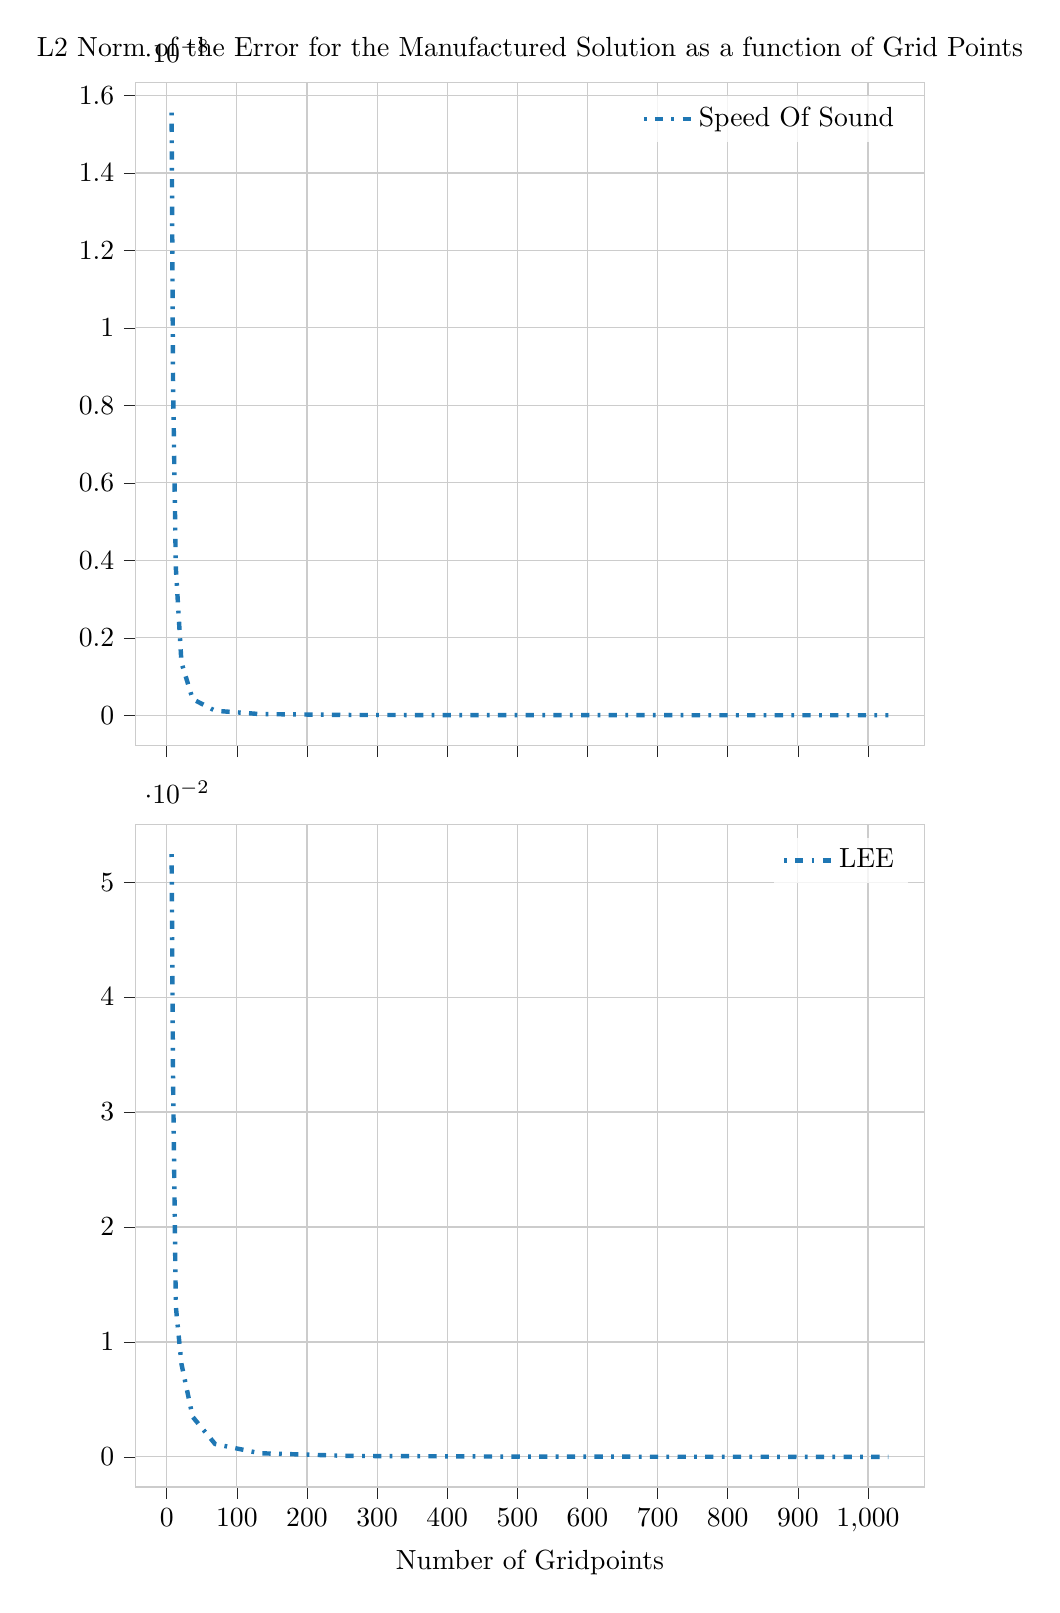
\begin{tikzpicture}

\definecolor{color0}{rgb}{0.12156862745098,0.466666666666667,0.705882352941177}

\begin{groupplot}[group style={group size=1 by 2}]
\nextgroupplot[
axis line style={white!80!black},
height=10cm,
legend cell align={left},
legend style={fill opacity=0.8, draw opacity=1, text opacity=1, draw=none},
scaled x ticks=manual:{}{\pgfmathparse{#1}},
tick align=outside,
tick pos=left,
title={L2 Norm of the Error for the Manufactured Solution as a function of Grid Points},
x grid style={white!80!black},
xmajorgrids,
xmin=-44.1, xmax=1080.1,
xtick style={color=white!15!black},
xticklabels={},
y grid style={white!80!black},
ymajorgrids,
ymin=-7.7685e-10, ymax=1.633585e-08,
ytick style={color=white!15!black}
]
\addplot [ultra thick, color0, dash pattern=on 1pt off 3pt on 3pt off 3pt]
table {%
7 1.5558e-08
9 8.666e-09
13 3.813e-09
21 1.362e-09
37 4.18e-10
69 1.17e-10
133 3.1e-11
261 8e-12
517 2e-12
1029 1e-12
};
\addlegendentry{Speed Of Sound}

\nextgroupplot[
axis line style={white!80!black},
height=10cm,
legend cell align={left},
legend style={fill opacity=0.8, draw opacity=1, text opacity=1, draw=none},
tick align=outside,
tick pos=left,
x grid style={white!80!black},
xlabel={Number of Gridpoints},
xmajorgrids,
xmin=-44.1, xmax=1080.1,
xtick style={color=white!15!black},
y grid style={white!80!black},
ymajorgrids,
ymin=-0.0026154475271, ymax=0.0550457217991,
ytick style={color=white!15!black}
]
\addplot [ultra thick, color0, dash pattern=on 1pt off 3pt on 3pt off 3pt]
table {%
7 0.052424759557
9 0.033179291821
13 0.013097177537
21 0.008095953516
37 0.003486847524
69 0.001122800012
133 0.000317623946
261 8.4369909e-05
517 2.1733375e-05
1029 5.514715e-06
};
\addlegendentry{LEE}
\end{groupplot}

\end{tikzpicture}

%%    \newpage
%%    % This file was created with tikzplotlib v0.9.12.
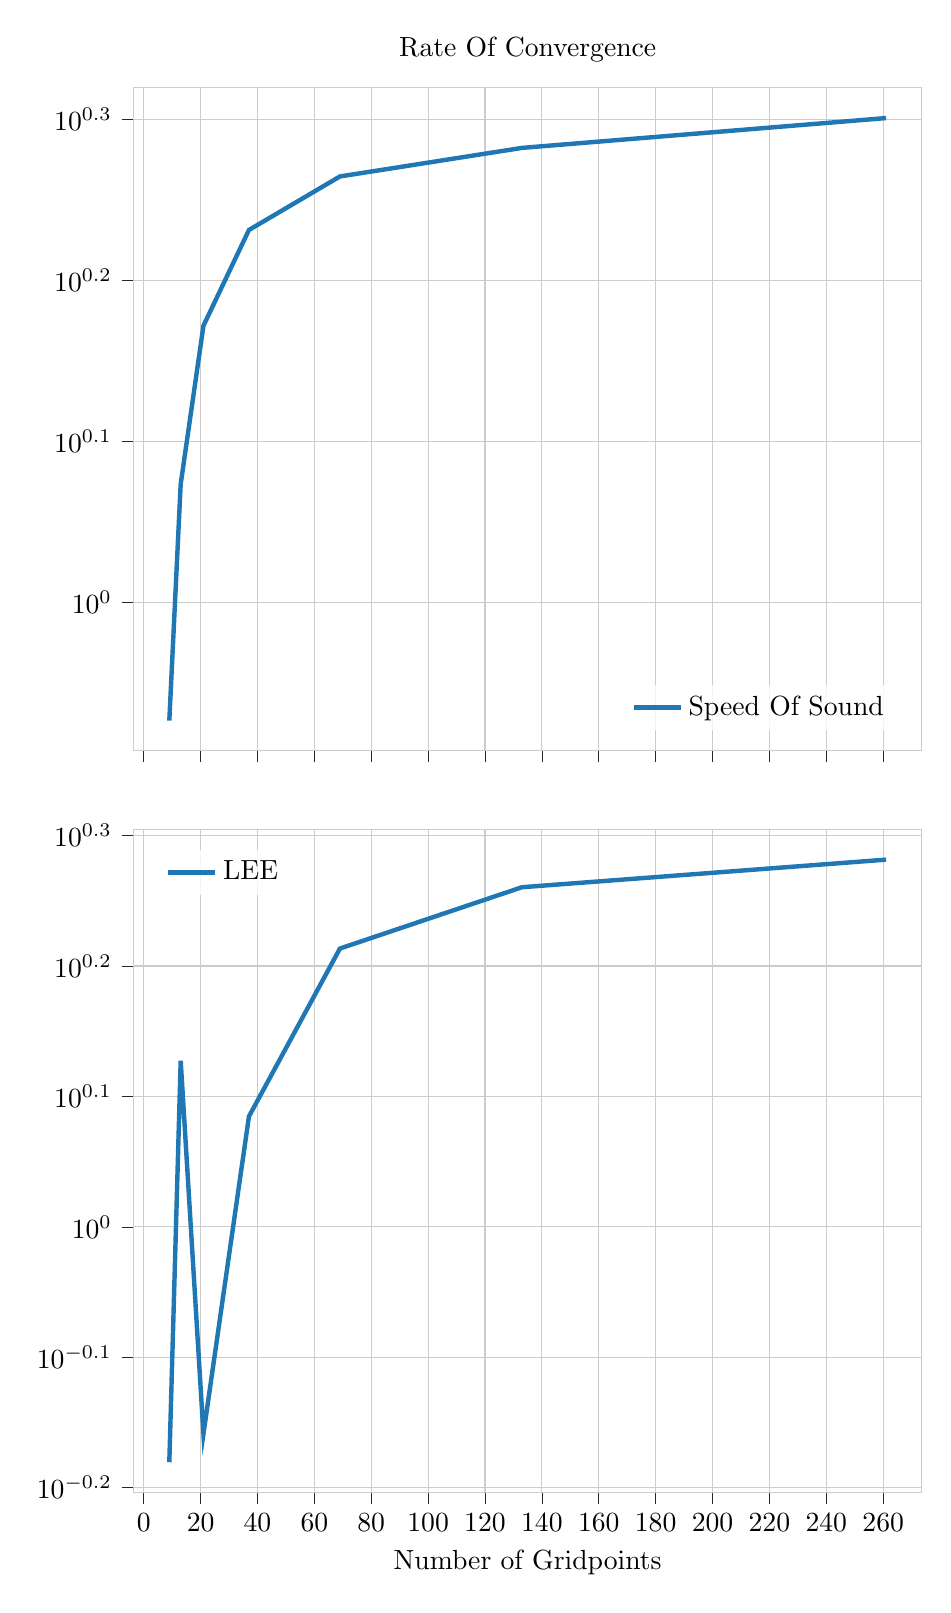
\begin{tikzpicture}

\definecolor{color0}{rgb}{0.12156862745098,0.466666666666667,0.705882352941177}

\begin{groupplot}[group style={group size=1 by 2}]
\nextgroupplot[
axis line style={white!80!black},
height=10cm,
legend cell align={left},
legend style={
  fill opacity=0.8,
  draw opacity=1,
  text opacity=1,
  at={(0.97,0.03)},
  anchor=south east,
  draw=none
},
log basis y={10},
scaled x ticks=manual:{}{\pgfmathparse{#1}},
tick align=outside,
tick pos=left,
title={Rate Of Convergence},
x grid style={white!80!black},
xmajorgrids,
xmin=-3.6, xmax=273.6,
xtick style={color=white!15!black},
xticklabels={},
y grid style={white!80!black},
ymajorgrids,
ymin=0.808580357974222, ymax=2.08813653136233,
ymode=log,
ytick style={color=white!15!black}
]
\addplot [ultra thick, color0]
table {%
9 0.844213092014
13 1.184345418732
21 1.485678426451
37 1.70393218834
69 1.839783697645
133 1.9164330736
261 2
};
\addlegendentry{Speed Of Sound}

\nextgroupplot[
axis line style={white!80!black},
height=10cm,
legend cell align={left},
legend style={
  fill opacity=0.8,
  draw opacity=1,
  text opacity=1,
  at={(0.03,0.97)},
  anchor=north west,
  draw=none
},
log basis y={10},
tick align=outside,
tick pos=left,
x grid style={white!80!black},
xlabel={Number of Gridpoints},
xmajorgrids,
xmin=-3.6, xmax=273.6,
xtick style={color=white!15!black},
y grid style={white!80!black},
ymajorgrids,
ymin=0.625773011285144, ymax=2.01701926788512,
ymode=log,
ytick style={color=white!15!black}
]
\addplot [ultra thick, color0]
table {%
9 0.659965245766
13 1.341027151607
21 0.693983030407
37 1.215277728398
69 1.63482229427
133 1.82170939735
261 1.912519226099
};
\addlegendentry{LEE}
\end{groupplot}

\end{tikzpicture}
 
%%    \newpage
%%    % This file was created with tikzplotlib v0.9.12.
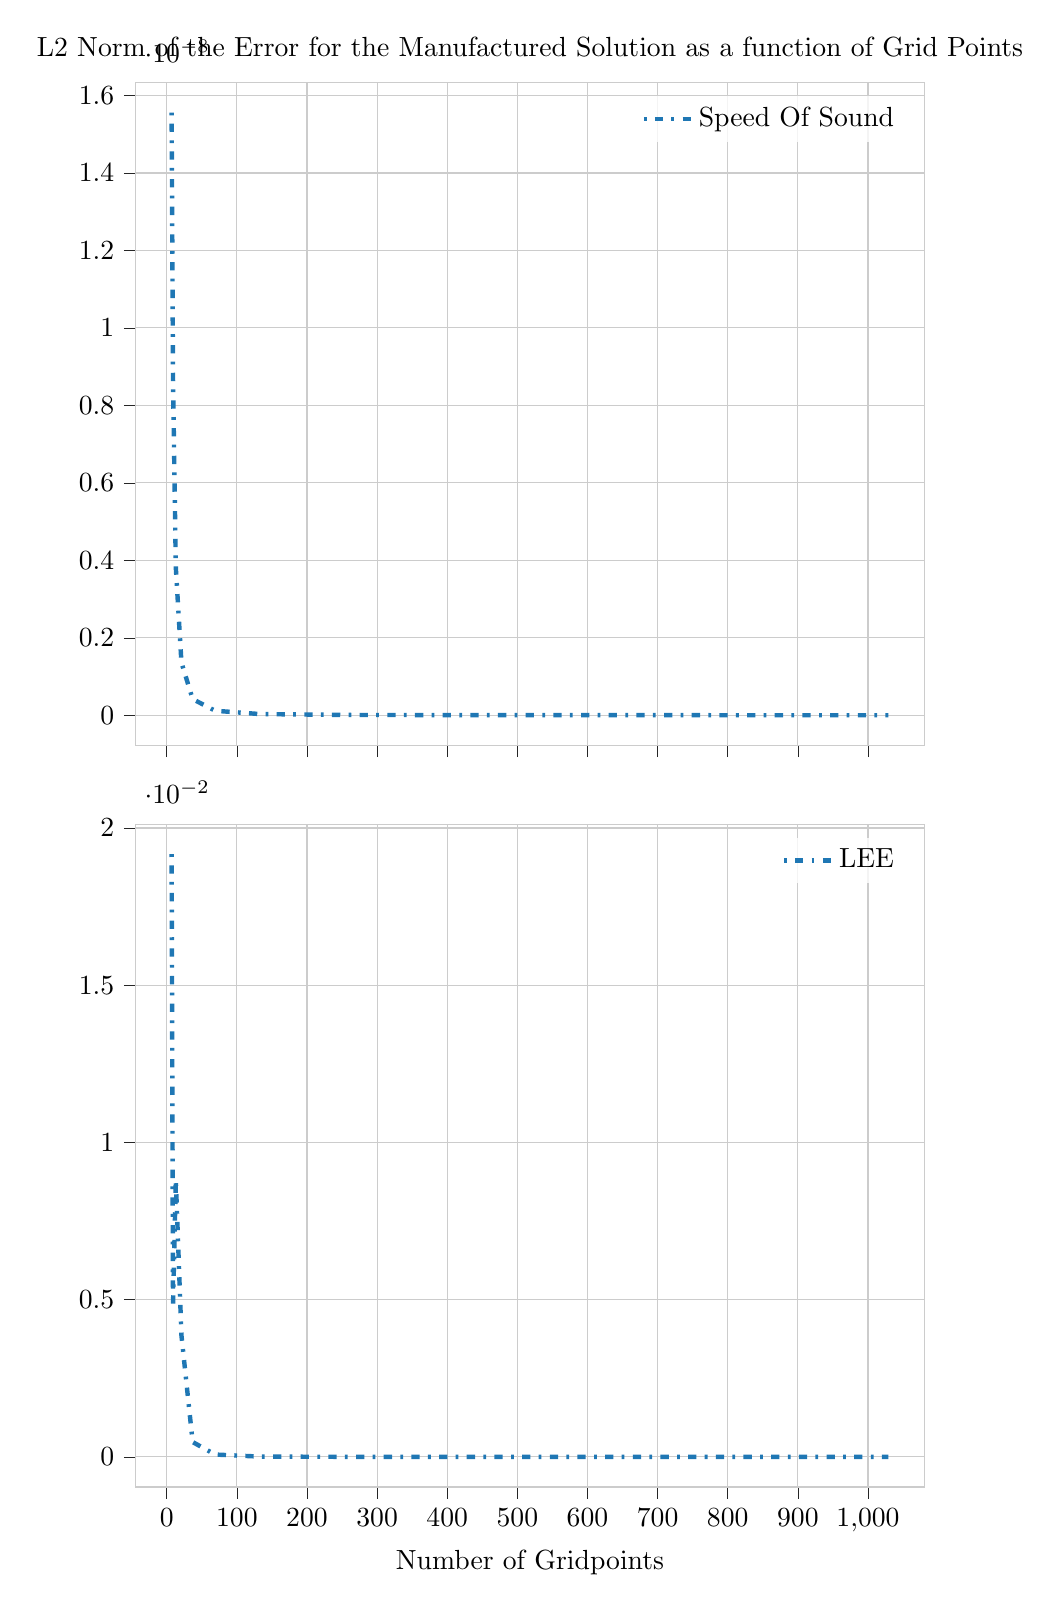
\begin{tikzpicture}

\definecolor{color0}{rgb}{0.12156862745098,0.466666666666667,0.705882352941177}

\begin{groupplot}[group style={group size=1 by 2}]
\nextgroupplot[
axis line style={white!80!black},
height=10cm,
legend cell align={left},
legend style={fill opacity=0.8, draw opacity=1, text opacity=1, draw=none},
scaled x ticks=manual:{}{\pgfmathparse{#1}},
tick align=outside,
tick pos=left,
title={L2 Norm of the Error for the Manufactured Solution as a function of Grid Points},
x grid style={white!80!black},
xmajorgrids,
xmin=-44.1, xmax=1080.1,
xtick style={color=white!15!black},
xticklabels={},
y grid style={white!80!black},
ymajorgrids,
ymin=-7.7685e-10, ymax=1.633585e-08,
ytick style={color=white!15!black}
]
\addplot [ultra thick, color0, dash pattern=on 1pt off 3pt on 3pt off 3pt]
table {%
7 1.5558e-08
9 8.666e-09
13 3.813e-09
21 1.362e-09
37 4.18e-10
69 1.17e-10
133 3.1e-11
261 8e-12
517 2e-12
1029 1e-12
};
\addlegendentry{Speed Of Sound}

\nextgroupplot[
axis line style={white!80!black},
height=10cm,
legend cell align={left},
legend style={fill opacity=0.8, draw opacity=1, text opacity=1, draw=none},
tick align=outside,
tick pos=left,
x grid style={white!80!black},
xlabel={Number of Gridpoints},
xmajorgrids,
xmin=-44.1, xmax=1080.1,
xtick style={color=white!15!black},
y grid style={white!80!black},
ymajorgrids,
ymin=-0.0009582683507, ymax=0.0201236873067,
ytick style={color=white!15!black}
]
\addplot [ultra thick, color0, dash pattern=on 1pt off 3pt on 3pt off 3pt]
table {%
7 0.019165416595
9 0.004802564507
13 0.008812127118
21 0.003866293269
37 0.00047117781
69 7.3167775e-05
133 7.230385e-06
261 5.50474e-07
517 3.6845e-08
1029 2.361e-09
};
\addlegendentry{LEE}
\end{groupplot}

\end{tikzpicture}

%%    \newpage
%%    % This file was created with tikzplotlib v0.9.12.
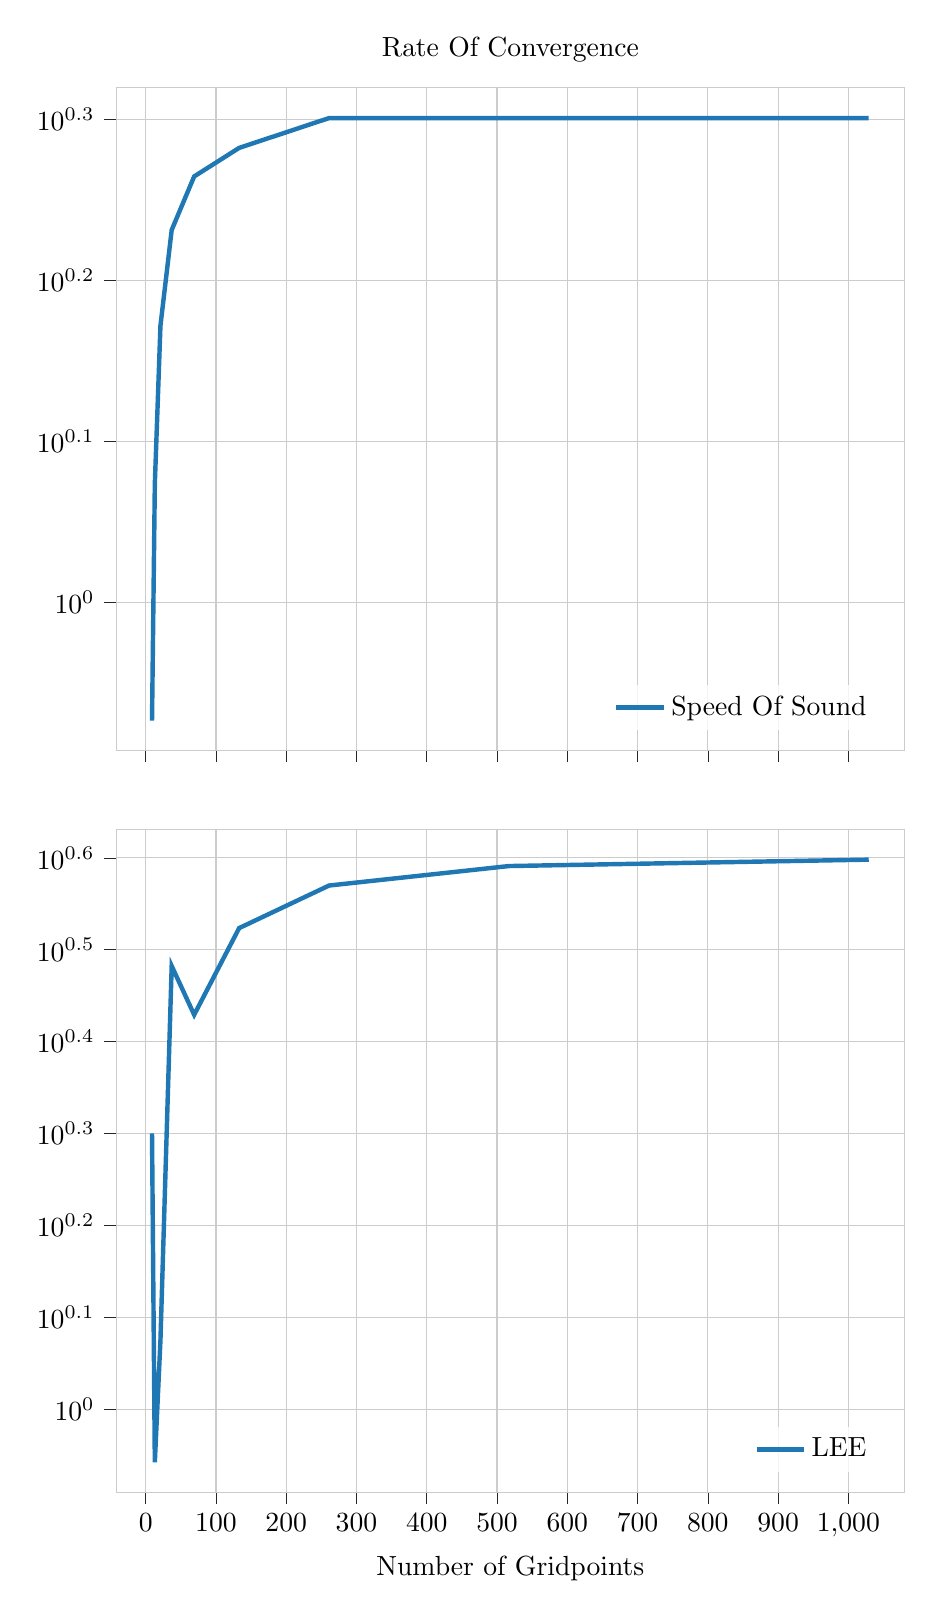
\begin{tikzpicture}

\definecolor{color0}{rgb}{0.12156862745098,0.466666666666667,0.705882352941177}

\begin{groupplot}[group style={group size=1 by 2}]
\nextgroupplot[
axis line style={white!80!black},
height=10cm,
legend cell align={left},
legend style={
  fill opacity=0.8,
  draw opacity=1,
  text opacity=1,
  at={(0.97,0.03)},
  anchor=south east,
  draw=none
},
log basis y={10},
scaled x ticks=manual:{}{\pgfmathparse{#1}},
tick align=outside,
tick pos=left,
title={Rate Of Convergence},
x grid style={white!80!black},
xmajorgrids,
xmin=-42, xmax=1080,
xtick style={color=white!15!black},
xticklabels={},
y grid style={white!80!black},
ymajorgrids,
ymin=0.808580357974222, ymax=2.08813653136233,
ymode=log,
ytick style={color=white!15!black}
]
\addplot [ultra thick, color0]
table {%
9 0.844213092014
13 1.184345418732
21 1.485678426451
37 1.70393218834
69 1.839783697645
133 1.9164330736
261 2
517 2
1029 2
};
\addlegendentry{Speed Of Sound}

\nextgroupplot[
axis line style={white!80!black},
height=10cm,
legend cell align={left},
legend style={
  fill opacity=0.8,
  draw opacity=1,
  text opacity=1,
  at={(0.97,0.03)},
  anchor=south east,
  draw=none
},
log basis y={10},
tick align=outside,
tick pos=left,
x grid style={white!80!black},
xlabel={Number of Gridpoints},
xmajorgrids,
xmin=-42, xmax=1080,
xtick style={color=white!15!black},
y grid style={white!80!black},
ymajorgrids,
ymin=0.812004202465992, ymax=4.27497570729649,
ymode=log,
ytick style={color=white!15!black}
]
\addplot [ultra thick, color0]
table {%
9 1.996628461096
13 0.875685314746
21 1.188539232462
37 3.036607570174
69 2.686991297944
133 3.339064044144
261 3.715326780136
517 3.901130812285
1029 3.964093243669
};
\addlegendentry{LEE}
\end{groupplot}

\end{tikzpicture}
 
%%

%    The method of manufactured solutions was used to determine the rate of convergence 
%    for SWIRL's numerical integration and finite difference methods while 
%    making sure all of the variables are set to a value to ensure all terms in 
%    the aerodynamic and aeroacoustic model were tested. This established a 
%    metric for determining whether SWIRL is working as intended. Figure [1] 
%    shows the ``manufactured'' velocity profile used to conduct the MMS. A series of 
%    hyperbolic tangents were summed together using the formulation described in 
%    Chapter 4. This method was used to create slope changes in the velocity profile
%    at various points along the radius in order to create a substantial amount of
%    error when a small number of grid points are used. Since SWIRL is a subsonic
%    code, the velocity profile was restricted such that the total mach number 
%    did not exceed one. The results from applying the trapezoidal rule to 
%    numerically integrate the tangential mach number to obtain the speed of sound
%    is reported in Figure [3]. The expected speed of sound was obtained by using 
%    the methods outlined in Chapter 4 and the actual speed of sound is the result 
%    obtained from SWIRL's output.

%    Figure [2] reports the manufactured functions used for the
%    perturbation variables. These functions were used to calculate the source terms
%    for the linearized euler equations which is reported in Figure [4]. The boundary
%    conditions implemented in SWIRL have also been applied to the 
%    manufactured radial velocity and pressure perturbations by implementing the 
%    fairing function method outlined in Chapter 4. After the source terms have 
%    been computed,     The L2Norm of the difference between the actual and expected speed of sound 
%    and source terms are shown in Figure [5]. An asymptotic rate of convergence 
%    was calculated for 10 iterations by recomputing the L2 norm of the error at 
%    progressively denser grids. For this study, the  grid spacing was halved 
%    each iteration.The results for a trapezoidal rule and a second-order central
%    finite difference scheme reported in Figure [6].  For the speed of sound, the
%    L2norm reached $10e-11$ (machine precision) in 8 iterations while the LEE 
%    is nearly converged but not yet at machine precison after 10 iterations. 

%    Figure [8] show the L2 norm for the speed of sound integration used to


%    %\begin{figure}
%    %\end{figure}
%    %\begin{figure}
%    %\end{figure}
%    %\begin{figure}
%    %    %\end{figure}
%    %\begin{figure}
%    %    %\end{figure}
%    %\begin{figure}
%    %\end{figure}
%    %
%    \section{Validation}
%    \subsection{Comparison to Kousen}


%There are four key test cases to run and make sure that the data is post processed 
%for.
%\begin{itemize}
%    \item Kousen's Test Cases
%        \subitem Cylinder, Uniform Flow with Liner (Table 4.3)
%        \begin{align*}
%            m &= 2 \\
%            k &= \frac{\omega r_T}{A_T} = -1 \\
%            M_x &= 0.5 \\
%            \eta_T &= 0.72 + 0.42i\\
%            \text{Confirm if 32 grid points is enough}
%        \end{align*} 
%        \subitem Cylinder, Shear Flow without Liner (Table 4.4)
%        \begin{align*}
%            m &= 0 \\
%            kb &= \left(\frac{\omega r_T}{A_T}\right)b = 20 \\
%            b &= r_{max} - r_{min} \\
%            \tilde{r} = \frac{r}{b} \\
%            M_x &= 0.3(1-\tilde{r})^{\frac{1}{7}} \\
%            \eta_T &= 0\\
%            \text{Confirm if 32 grid points is enough}
%        \end{align*}
%        \subitem Annulus, Shear Flow without Liner (Table 4.5)
%        \begin{align*}
%            m &= 0 \\
%            kb &= \left(\frac{\omega r_T}{A_T}\right)b = 10 \\
%            b &= r_{max} - r_{min}  = \frac{1}{7}\\
%            k &= 70 \\
%            \tilde{r} = \frac{r}{b} = 6.0 \\
%            M_x &= 0.3\left(1 - 2 \left| \frac{r_{max}-r}{b} + 0.5 \right|  \right)^{\frac{1}{7}} \\
%            \eta_T &= 0\\
%            \text{Confirm if 32 grid points is enough}
%        \end{align*}
%        \subitem Annulus, Shear Flow with Liner (Table 4.6)
%        \begin{align*}
%            m &= 0 \\
%            kb &= \left(\frac{\omega r_T}{A_T}\right)b = 10 \\
%            b &= r_{max} - r_{min}  = \frac{1}{3}\\
%            k &= 30 \\
%            \tilde{r} = \frac{r}{b} = 2.0 \\
%            M_x &= 0.3\left(1 - 2 \left| \frac{r_{max}-r}{b} + 0.5 \right|  \right)^{\frac{1}{7}} \\
%            \eta_T &= 0.3 + 0.1i\\
%            \text{Confirm if 32 grid points is enough}
%        \end{align*}
%\end{itemize}
%\subsubsection{Test Case 1}
%\begin{figure}[h!]
%    \centering
%    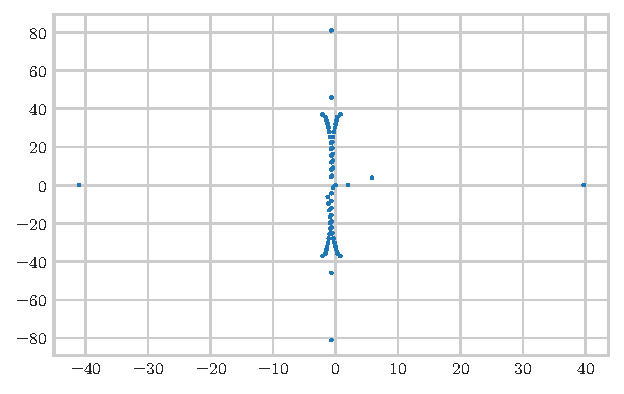
\includegraphics[width=\textwidth]{Chapter-5-Results/tex-outputs/gam.acc.scatter.pdf}
%    \caption{i}
%\end{figure}
%\begin{tiny}
% \begin{figure}
%     \centering
%     \begin{tabular}{rrrrrrr}
\toprule
   \# &          j &       Re\{gam\} &   Im\{gam\} &     Re\{gam\}/k &  Im\{gam\}/k &         kappa \\
\midrule
   1 &  89.888193 & -4.294270e+02 &  2.996273 & -1.431423e+01 &   0.014009 &  6.692806e-02 \\
   2 & -44.105475 &  3.903668e+02 & -1.470182 &  1.301223e+01 &  -0.008574 & -7.588213e-02 \\
   3 &  -7.496128 &  4.378636e+02 & -0.249871 &  1.459545e+01 &  -0.001173 & -6.849442e-02 \\
   4 &  -7.496128 & -4.378636e+02 & -0.249871 & -1.459545e+01 &  -0.001173 &  6.849442e-02 \\
   5 &  -9.774676 &  3.855793e+02 & -0.325823 &  1.285264e+01 &  -0.001971 & -7.775505e-02 \\
   6 &  -8.438677 &  3.855866e+02 & -0.281289 &  1.285289e+01 &  -0.001702 & -7.776629e-02 \\
   7 &  -9.761835 &  3.852503e+02 & -0.325395 &  1.284168e+01 &  -0.001972 & -7.782149e-02 \\
   8 &  -8.465671 &  3.852805e+02 & -0.282189 &  1.284268e+01 &  -0.001710 & -7.782778e-02 \\
   9 &  -9.733025 &  3.846870e+02 & -0.324434 &  1.282290e+01 &  -0.001972 & -7.793558e-02 \\
  10 &  -8.511308 &  3.847621e+02 & -0.283710 &  1.282540e+01 &  -0.001724 & -7.793213e-02 \\
  11 &  -9.685318 &  3.839076e+02 & -0.322844 &  1.279692e+01 &  -0.001970 & -7.809409e-02 \\
  12 &  -8.563984 &  3.840575e+02 & -0.285466 &  1.280192e+01 &  -0.001741 & -7.807448e-02 \\
  13 &  -8.600791 &  3.831817e+02 & -0.286693 &  1.277272e+01 &  -0.001756 & -7.825242e-02 \\
  14 &  -9.604853 &  3.829203e+02 & -0.320162 &  1.276401e+01 &  -0.001964 & -7.829601e-02 \\
  15 &  -8.586041 &  3.821334e+02 & -0.286201 &  1.273778e+01 &  -0.001763 & -7.846700e-02 \\
  16 &  -9.445636 &  3.817146e+02 & -0.314855 &  1.272382e+01 &  -0.001944 & -7.854465e-02 \\
  17 &  -6.597191 &  3.814637e+02 & -0.219906 &  1.271546e+01 &  -0.001360 & -7.862092e-02 \\
  18 &  -6.625845 &  3.812113e+02 & -0.220862 &  1.270704e+01 &  -0.001367 & -7.867274e-02 \\
  19 &  -6.701045 &  3.806134e+02 & -0.223368 &  1.268711e+01 &  -0.001387 & -7.879572e-02 \\
  20 &  -8.786507 &  3.815498e+02 & -0.292884 &  1.271833e+01 &  -0.001810 & -7.858503e-02 \\
  21 &  -8.938402 &  3.813608e+02 & -0.297947 &  1.271203e+01 &  -0.001843 & -7.862247e-02 \\
  22 &  -8.491807 &  3.808811e+02 & -0.283060 &  1.269604e+01 &  -0.001755 & -7.872560e-02 \\
  23 &  -8.950208 &  3.808982e+02 & -0.298340 &  1.269661e+01 &  -0.001850 & -7.871774e-02 \\
  24 &  -6.803918 &  3.797954e+02 & -0.226797 &  1.265985e+01 &  -0.001415 & -7.896456e-02 \\
  25 &  -9.166327 &  3.802584e+02 & -0.305544 &  1.267528e+01 &  -0.001901 & -7.884791e-02 \\
  26 &  -9.173251 &  3.800929e+02 & -0.305775 &  1.266976e+01 &  -0.001904 & -7.888212e-02 \\
  27 &  -6.934558 &  3.787513e+02 & -0.231152 &  1.262504e+01 &  -0.001450 & -7.918111e-02 \\
  28 &  -8.332473 &  3.793839e+02 & -0.277749 &  1.264613e+01 &  -0.001736 & -7.903744e-02 \\
  29 &  -9.034080 &  3.792619e+02 & -0.301136 &  1.264206e+01 &  -0.001883 & -7.905615e-02 \\
  30 &  -9.243824 &  3.785435e+02 & -0.308127 &  1.261812e+01 &  -0.001934 & -7.920389e-02 \\
  31 &  -9.117376 &  3.779165e+02 & -0.303913 &  1.259722e+01 &  -0.001914 & -7.933644e-02 \\
  32 &  -7.103169 &  3.774775e+02 & -0.236772 &  1.258258e+01 &  -0.001495 & -7.944680e-02 \\
  33 &  -8.137999 &  3.776425e+02 & -0.271267 &  1.258808e+01 &  -0.001711 & -7.940335e-02 \\
  34 &  -9.154154 &  3.769665e+02 & -0.305138 &  1.256555e+01 &  -0.001931 & -7.953577e-02 \\
  35 &  -9.210755 &  3.762096e+02 & -0.307025 &  1.254032e+01 &  -0.001951 & -7.969501e-02 \\
  36 &  -7.309795 &  3.760254e+02 & -0.243660 &  1.253418e+01 &  -0.001550 & -7.975171e-02 \\
  37 &  -7.927507 &  3.756349e+02 & -0.264250 &  1.252116e+01 &  -0.001685 & -7.982923e-02 \\
  38 &  -9.130224 &  3.752038e+02 & -0.304341 &  1.250679e+01 &  -0.001945 & -7.990923e-02 \\
  39 &  -7.431607 &  3.743389e+02 & -0.247720 &  1.247796e+01 &  -0.001590 & -8.010971e-02 \\
  40 &  -9.225306 &  3.742433e+02 & -0.307510 &  1.247478e+01 &  -0.001975 & -8.011307e-02 \\
  41 &  -7.829935 &  3.734354e+02 & -0.260998 &  1.244785e+01 &  -0.001684 & -8.029988e-02 \\
  42 &  -9.141885 &  3.731942e+02 & -0.304730 &  1.243981e+01 &  -0.001968 & -8.033889e-02 \\
  43 &  -7.544257 &  3.723158e+02 & -0.251475 &  1.241053e+01 &  -0.001632 & -8.054368e-02 \\
  44 &  -9.208751 &  3.720686e+02 & -0.306958 &  1.240229e+01 &  -0.001994 & -8.058093e-02 \\
  45 &  -7.783693 &  3.711331e+02 & -0.259456 &  1.237110e+01 &  -0.001695 & -8.079799e-02 \\
  46 &  -9.158631 &  3.709360e+02 & -0.305288 &  1.236453e+01 &  -0.001996 & -8.082721e-02 \\
  47 &  -7.649711 &  3.699938e+02 & -0.254990 &  1.233313e+01 &  -0.001676 & -8.104780e-02 \\
  48 &  -9.187835 &  3.696824e+02 & -0.306261 &  1.232275e+01 &  -0.002016 & -8.110065e-02 \\
  49 &  -7.773142 &  3.686620e+02 & -0.259105 &  1.228873e+01 &  -0.001715 & -8.133918e-02 \\
  50 &  -9.166527 &  3.684400e+02 & -0.305551 &  1.228133e+01 &  -0.002025 & -8.137402e-02 \\
  51 &  -7.729486 &  3.674157e+02 & -0.257650 &  1.224719e+01 &  -0.001717 & -8.161527e-02 \\
  52 &  -9.168798 &  3.670777e+02 & -0.305627 &  1.223592e+01 &  -0.002040 & -8.167560e-02 \\
  53 &  -7.789659 &  3.659850e+02 & -0.259655 &  1.219950e+01 &  -0.001744 & -8.193344e-02 \\
  54 &  -9.163034 &  3.657162e+02 & -0.305434 &  1.219054e+01 &  -0.002054 & -8.197935e-02 \\
  55 &  -7.789972 &  3.646110e+02 & -0.259666 &  1.215370e+01 &  -0.001757 & -8.224193e-02 \\
  56 &  -9.150402 &  3.642518e+02 & -0.305013 &  1.214173e+01 &  -0.002068 & -8.230867e-02 \\
  57 &  -7.822310 &  3.630910e+02 & -0.260744 &  1.210303e+01 &  -0.001779 & -8.258559e-02 \\
  58 &  -9.149632 &  3.627708e+02 & -0.304988 &  1.209236e+01 &  -0.002084 & -8.264427e-02 \\
  59 &  -7.841903 &  3.615912e+02 & -0.261397 &  1.205304e+01 &  -0.001798 & -8.292763e-02 \\
  60 &  -9.129961 &  3.612045e+02 & -0.304332 &  1.204015e+01 &  -0.002098 & -8.300241e-02 \\
  61 &  -7.864480 &  3.599793e+02 & -0.262149 &  1.199931e+01 &  -0.001820 & -8.329836e-02 \\
  62 &  -9.128015 &  3.596070e+02 & -0.304267 &  1.198690e+01 &  -0.002116 & -8.337070e-02 \\
  63 &  -7.892046 &  3.583603e+02 & -0.263068 &  1.194534e+01 &  -0.001843 & -8.367406e-02 \\
  64 &  -9.105235 &  3.579374e+02 & -0.303508 &  1.193125e+01 &  -0.002131 & -8.375933e-02 \\
  65 &  -7.913048 &  3.566529e+02 & -0.263768 &  1.188843e+01 &  -0.001865 & -8.407401e-02 \\
  66 &  -9.099177 &  3.562266e+02 & -0.303306 &  1.187422e+01 &  -0.002150 & -8.416116e-02 \\
  67 &  -7.943974 &  3.549207e+02 & -0.264799 &  1.183069e+01 &  -0.001891 & -8.448359e-02 \\
  68 &  -9.074759 &  3.544524e+02 & -0.302492 &  1.181508e+01 &  -0.002165 & -8.458215e-02 \\
  69 &  -7.966760 &  3.531155e+02 & -0.265559 &  1.177052e+01 &  -0.001916 & -8.491481e-02 \\
  70 &  -9.063560 &  3.526309e+02 & -0.302119 &  1.175436e+01 &  -0.002185 & -8.501863e-02 \\
  71 &  -7.999389 &  3.512753e+02 & -0.266646 &  1.170918e+01 &  -0.001944 & -8.535884e-02 \\
  72 &  -9.037810 &  3.507512e+02 & -0.301260 &  1.169171e+01 &  -0.002202 & -8.547396e-02 \\
  73 &  -8.025022 &  3.493715e+02 & -0.267501 &  1.164572e+01 &  -0.001971 & -8.582319e-02 \\
  74 &  -9.021516 &  3.488207e+02 & -0.300717 &  1.162736e+01 &  -0.002223 & -8.594658e-02 \\
  75 &  -8.058690 &  3.474273e+02 & -0.268623 &  1.158091e+01 &  -0.002002 & -8.630257e-02 \\
  76 &  -8.994495 &  3.468348e+02 & -0.299817 &  1.156116e+01 &  -0.002242 & -8.643837e-02 \\
  77 &  -8.086947 &  3.454256e+02 & -0.269565 &  1.151419e+01 &  -0.002032 & -8.680181e-02 \\
  78 &  -8.973919 &  3.447965e+02 & -0.299131 &  1.149322e+01 &  -0.002263 & -8.694893e-02 \\
  79 &  -8.120879 &  3.433807e+02 & -0.270696 &  1.144602e+01 &  -0.002065 & -8.731775e-02 \\
  80 &  -8.946125 &  3.427043e+02 & -0.298204 &  1.142348e+01 &  -0.002284 & -8.747942e-02 \\
  81 &  -8.150494 &  3.412823e+02 & -0.271683 &  1.137608e+01 &  -0.002098 & -8.785367e-02 \\
  82 &  -8.922888 &  3.405590e+02 & -0.297430 &  1.135197e+01 &  -0.002306 & -8.803003e-02 \\
  83 &  -8.183282 &  3.391392e+02 & -0.272776 &  1.130464e+01 &  -0.002133 & -8.840778e-02 \\
  84 &  -8.895603 &  3.383608e+02 & -0.296520 &  1.127869e+01 &  -0.002329 & -8.860152e-02 \\
  85 &  -8.212225 &  3.369449e+02 & -0.273741 &  1.123150e+01 &  -0.002169 & -8.898248e-02 \\
  86 &  -8.871973 &  3.361101e+02 & -0.295732 &  1.120367e+01 &  -0.002354 & -8.919433e-02 \\
  87 &  -8.242159 &  3.347047e+02 & -0.274739 &  1.115682e+01 &  -0.002206 & -8.957692e-02 \\
  88 &  -8.846859 &  3.338077e+02 & -0.294895 &  1.112692e+01 &  -0.002380 & -8.980903e-02 \\
  89 &  -8.268568 &  3.324144e+02 & -0.275619 &  1.108048e+01 &  -0.002243 & -9.019299e-02 \\
  90 &  -8.824865 &  3.314540e+02 & -0.294162 &  1.104847e+01 &  -0.002408 & -9.044617e-02 \\
  91 &  -8.294645 &  3.300772e+02 & -0.276488 &  1.100257e+01 &  -0.002283 & -9.083048e-02 \\
  92 &  -8.802923 &  3.290504e+02 & -0.293431 &  1.096835e+01 &  -0.002437 & -9.110624e-02 \\
  93 &  -8.317743 &  3.276903e+02 & -0.277258 &  1.092301e+01 &  -0.002322 & -9.149092e-02 \\
  94 &  -8.783466 &  3.265971e+02 & -0.292782 &  1.088657e+01 &  -0.002469 & -9.178992e-02 \\
  95 &  -8.340030 &  3.252558e+02 & -0.278001 &  1.084186e+01 &  -0.002363 & -9.217449e-02 \\
  96 &  -8.764648 &  3.240953e+02 & -0.292155 &  1.080318e+01 &  -0.002501 & -9.249773e-02 \\
  97 &  -8.360008 &  3.227723e+02 & -0.278667 &  1.075908e+01 &  -0.002406 & -9.288248e-02 \\
  98 &  -8.747631 &  3.215451e+02 & -0.291588 &  1.071817e+01 &  -0.002536 & -9.323052e-02 \\
  99 &  -8.379130 &  3.202410e+02 & -0.279304 &  1.067470e+01 &  -0.002449 & -9.361535e-02 \\
 100 &  -8.731345 &  3.189476e+02 & -0.291045 &  1.063159e+01 &  -0.002573 & -9.398890e-02 \\
 101 &  -8.396526 &  3.176614e+02 & -0.279884 &  1.058871e+01 &  -0.002495 & -9.437426e-02 \\
 102 &  -8.716302 &  3.163028e+02 & -0.290543 &  1.054343e+01 &  -0.002612 & -9.477385e-02 \\
 103 &  -8.413152 &  3.150343e+02 & -0.280438 &  1.050114e+01 &  -0.002541 & -9.515985e-02 \\
 104 &  -8.701918 &  3.136117e+02 & -0.290064 &  1.045372e+01 &  -0.002652 & -9.558610e-02 \\
 105 &  -8.428475 &  3.123597e+02 & -0.280949 &  1.041199e+01 &  -0.002590 & -9.597325e-02 \\
 106 &  -8.688395 &  3.108742e+02 & -0.289613 &  1.036247e+01 &  -0.002695 & -9.642673e-02 \\
 107 &  -8.443120 &  3.096382e+02 & -0.281437 &  1.032127e+01 &  -0.002640 & -9.681527e-02 \\
 108 &  -8.675435 &  3.080911e+02 & -0.289181 &  1.026970e+01 &  -0.002740 & -9.729663e-02 \\
 109 &  -8.456747 &  3.068700e+02 & -0.281892 &  1.022900e+01 &  -0.002692 & -9.768707e-02 \\
 110 &  -8.663097 &  3.052626e+02 & -0.288770 &  1.017542e+01 &  -0.002787 & -9.819696e-02 \\
 111 &  -8.469763 &  3.040557e+02 & -0.282325 &  1.013519e+01 &  -0.002746 & -9.858964e-02 \\
 112 &  -8.651245 &  3.023892e+02 & -0.288375 &  1.007964e+01 &  -0.002836 & -9.912876e-02 \\
 113 &  -8.481945 &  3.011955e+02 & -0.282731 &  1.003985e+01 &  -0.002803 & -9.952417e-02 \\
 114 &  -8.639872 &  2.994711e+02 & -0.287996 &  9.982371e+00 &  -0.002888 & -1.000933e-01 \\
 115 &  -8.493557 &  2.982899e+02 & -0.283119 &  9.942997e+00 &  -0.002861 & -1.004918e-01 \\
 116 &  -8.628931 &  2.965090e+02 & -0.287631 &  9.883632e+00 &  -0.002942 & -1.010918e-01 \\
 117 &  -8.504454 &  2.953394e+02 & -0.283482 &  9.844645e+00 &  -0.002923 & -1.014939e-01 \\
 118 &  -8.618389 &  2.935029e+02 & -0.287280 &  9.783430e+00 &  -0.002999 & -1.021256e-01 \\
 119 &  -8.514807 &  2.923443e+02 & -0.283827 &  9.744811e+00 &  -0.002986 & -1.025317e-01 \\
 120 &  -8.608241 &  2.904535e+02 & -0.286941 &  9.681784e+00 &  -0.003058 & -1.031961e-01 \\
 121 &  -8.524517 &  2.893052e+02 & -0.284151 &  9.643506e+00 &  -0.003053 & -1.036068e-01 \\
 122 &  -8.598447 &  2.873611e+02 & -0.286615 &  9.578703e+00 &  -0.003121 & -1.043049e-01 \\
 123 &  -8.533699 &  2.862224e+02 & -0.284457 &  9.540748e+00 &  -0.003122 & -1.047205e-01 \\
 124 &  -8.589021 &  2.842261e+02 & -0.286301 &  9.474203e+00 &  -0.003187 & -1.054535e-01 \\
 125 &  -8.542286 &  2.830965e+02 & -0.284743 &  9.436551e+00 &  -0.003195 & -1.058745e-01 \\
 126 &  -8.579925 &  2.810488e+02 & -0.285997 &  9.368294e+00 &  -0.003256 & -1.066436e-01 \\
 127 &  -8.550354 &  2.799279e+02 & -0.285012 &  9.330929e+00 &  -0.003270 & -1.070706e-01 \\
 128 &  -8.571180 &  2.778298e+02 & -0.285706 &  9.260993e+00 &  -0.003328 & -1.078771e-01 \\
 129 &  -8.557861 &  2.767170e+02 & -0.285262 &  9.223900e+00 &  -0.003350 & -1.083104e-01 \\
 130 &  -8.562747 &  2.745693e+02 & -0.285425 &  9.152311e+00 &  -0.003404 & -1.091559e-01 \\
 131 &  -8.564855 &  2.734643e+02 & -0.285495 &  9.115477e+00 &  -0.003433 & -1.095960e-01 \\
 132 &  -8.554652 &  2.712679e+02 & -0.285155 &  9.042264e+00 &  -0.003484 & -1.104819e-01 \\
 133 &  -8.571314 &  2.701703e+02 & -0.285710 &  9.005678e+00 &  -0.003519 & -1.109294e-01 \\
 134 &  -8.546858 &  2.679259e+02 & -0.284895 &  8.930865e+00 &  -0.003568 & -1.118574e-01 \\
 135 &  -8.577264 &  2.668355e+02 & -0.285909 &  8.894515e+00 &  -0.003610 & -1.123128e-01 \\
 136 &  -8.539391 &  2.645438e+02 & -0.284646 &  8.818128e+00 &  -0.003657 & -1.132847e-01 \\
 137 &  -8.582703 &  2.634603e+02 & -0.286090 &  8.782009e+00 &  -0.003706 & -1.137484e-01 \\
 138 &  -8.532211 &  2.611220e+02 & -0.284407 &  8.704067e+00 &  -0.003750 & -1.147663e-01 \\
 139 &  -8.587636 &  2.600451e+02 & -0.286255 &  8.668170e+00 &  -0.003806 & -1.152389e-01 \\
 140 &  -8.525349 &  2.576609e+02 & -0.284178 &  8.588698e+00 &  -0.003848 & -1.163048e-01 \\
 141 &  -8.592081 &  2.565906e+02 & -0.286403 &  8.553020e+00 &  -0.003911 & -1.167868e-01 \\
 142 &  -8.518761 &  2.541610e+02 & -0.283959 &  8.472033e+00 &  -0.003952 & -1.179030e-01 \\
 143 &  -8.596023 &  2.530970e+02 & -0.286534 &  8.436568e+00 &  -0.004021 & -1.183950e-01 \\
 144 &  -8.512482 &  2.506227e+02 & -0.283749 &  8.354088e+00 &  -0.004061 & -1.195639e-01 \\
 145 &  -8.599502 &  2.495651e+02 & -0.286650 &  8.318838e+00 &  -0.004137 & -1.200665e-01 \\
 146 &  -8.506461 &  2.470463e+02 & -0.283549 &  8.234878e+00 &  -0.004176 & -1.212909e-01 \\
 147 &  -8.602476 &  2.459951e+02 & -0.286749 &  8.199837e+00 &  -0.004260 & -1.218047e-01 \\
 148 &  -8.500741 &  2.434325e+02 & -0.283358 &  8.114418e+00 &  -0.004298 & -1.230873e-01 \\
 149 &  -8.605018 &  2.423877e+02 & -0.286834 &  8.079591e+00 &  -0.004388 & -1.236129e-01 \\
 150 &  -8.495260 &  2.397816e+02 & -0.283175 &  7.992722e+00 &  -0.004427 & -1.249570e-01 \\
 151 &  -8.607045 &  2.387431e+02 & -0.286901 &  7.958103e+00 &  -0.004524 & -1.254950e-01 \\
 152 &  -8.490074 &  2.360942e+02 & -0.283002 &  7.869806e+00 &  -0.004564 & -1.269038e-01 \\
 153 &  -8.608682 &  2.350622e+02 & -0.286956 &  7.835406e+00 &  -0.004668 & -1.274549e-01 \\
 154 &  -8.485107 &  2.323705e+02 & -0.282837 &  7.745682e+00 &  -0.004708 & -1.289323e-01 \\
 155 &  -8.609781 &  2.313448e+02 & -0.286993 &  7.711495e+00 &  -0.004819 & -1.294972e-01 \\
 156 &  -8.480428 &  2.286111e+02 & -0.282681 &  7.620370e+00 &  -0.004861 & -1.310469e-01 \\
 157 &  -8.610543 &  2.275923e+02 & -0.287018 &  7.586410e+00 &  -0.004980 & -1.316263e-01 \\
 158 &  -8.475945 &  2.248164e+02 & -0.282532 &  7.493881e+00 &  -0.005024 & -1.332528e-01 \\
 159 &  -8.610730 &  2.238042e+02 & -0.287024 &  7.460139e+00 &  -0.005150 & -1.338476e-01 \\
 160 &  -8.471748 &  2.209870e+02 & -0.282392 &  7.366232e+00 &  -0.005197 & -1.355554e-01 \\
 161 &  -8.610652 &  2.199819e+02 & -0.287022 &  7.332730e+00 &  -0.005330 & -1.361662e-01 \\
 162 &  -8.467720 &  2.171231e+02 & -0.282257 &  7.237436e+00 &  -0.005380 & -1.379606e-01 \\
 163 &  -8.609937 &  2.161248e+02 & -0.286998 &  7.204161e+00 &  -0.005521 & -1.385887e-01 \\
 164 &  -8.463979 &  2.132253e+02 & -0.282133 &  7.107511e+00 &  -0.005576 & -1.404749e-01 \\
 165 &  -8.609053 &  2.122347e+02 & -0.286968 &  7.074490e+00 &  -0.005724 & -1.411207e-01 \\
 166 &  -8.460376 &  2.092940e+02 & -0.282013 &  6.976468e+00 &  -0.005785 & -1.431052e-01 \\
 167 &  -8.607438 &  2.083105e+02 & -0.286915 &  6.943683e+00 &  -0.005941 & -1.437703e-01 \\
 168 &  -8.457065 &  2.053298e+02 & -0.281902 &  6.844326e+00 &  -0.006008 & -1.458590e-01 \\
 169 &  -8.605786 &  2.043544e+02 & -0.286860 &  6.811814e+00 &  -0.006171 & -1.465439e-01 \\
 170 &  -8.453857 &  2.013328e+02 & -0.281795 &  6.711092e+00 &  -0.006246 & -1.487448e-01 \\
 171 &  -8.603263 &  2.003648e+02 & -0.286775 &  6.678828e+00 &  -0.006417 & -1.494513e-01 \\
 172 &  -8.450952 &  1.973037e+02 & -0.281698 &  6.576790e+00 &  -0.006501 & -1.517714e-01 \\
 173 &  -8.600885 &  1.963446e+02 & -0.286696 &  6.544820e+00 &  -0.006680 & -1.525000e-01 \\
 174 &  -8.448106 &  1.932427e+02 & -0.281604 &  6.441424e+00 &  -0.006774 & -1.549490e-01 \\
 175 &  -8.597432 &  1.922913e+02 & -0.286581 &  6.409711e+00 &  -0.006962 & -1.557020e-01 \\
 176 &  -8.445584 &  1.891505e+02 & -0.281519 &  6.305018e+00 &  -0.007068 & -1.582883e-01 \\
 177 &  -8.594373 &  1.882087e+02 & -0.286479 &  6.273623e+00 &  -0.007264 & -1.590659e-01 \\
 178 &  -8.443069 &  1.850272e+02 & -0.281436 &  6.167572e+00 &  -0.007383 & -1.618014e-01 \\
 179 &  -8.589952 &  1.840933e+02 & -0.286332 &  6.136443e+00 &  -0.007587 & -1.626068e-01 \\
 180 &  -8.440909 &  1.808734e+02 & -0.281364 &  6.029113e+00 &  -0.007724 & -1.655014e-01 \\
 181 &  -8.586265 &  1.799499e+02 & -0.286209 &  5.998330e+00 &  -0.007937 & -1.663344e-01 \\
 182 &  -8.438691 &  1.766891e+02 & -0.281290 &  5.889638e+00 &  -0.008091 & -1.694033e-01 \\
 183 &  -8.580815 &  1.757739e+02 & -0.286027 &  5.859128e+00 &  -0.008312 & -1.702681e-01 \\
 184 &  -8.436873 &  1.724752e+02 & -0.281229 &  5.749174e+00 &  -0.008488 & -1.735228e-01 \\
 185 &  -8.576560 &  1.715713e+02 & -0.285885 &  5.719042e+00 &  -0.008719 & -1.744186e-01 \\
 186 &  -8.434916 &  1.682314e+02 & -0.281164 &  5.607714e+00 &  -0.008919 & -1.778786e-01 \\
 187 &  -8.569994 &  1.673358e+02 & -0.285666 &  5.577860e+00 &  -0.009158 & -1.788112e-01 \\
 188 &  -8.436776 & -3.855888e+02 & -0.281226 & -1.285296e+01 &  -0.001702 &  7.776586e-02 \\
 189 &  -9.771946 & -3.855790e+02 & -0.325732 & -1.285263e+01 &  -0.001971 &  7.775512e-02 \\
 190 &  -8.455126 & -3.852845e+02 & -0.281838 & -1.284282e+01 &  -0.001708 &  7.782706e-02 \\
 191 &  -9.752123 & -3.852547e+02 & -0.325071 & -1.284182e+01 &  -0.001970 &  7.782070e-02 \\
 192 &  -8.488441 & -3.847679e+02 & -0.282948 & -1.282560e+01 &  -0.001719 &  7.793115e-02 \\
 193 &  -9.713437 & -3.846994e+02 & -0.323781 & -1.282331e+01 &  -0.001968 &  7.793328e-02 \\
 194 &  -8.526142 & -3.840646e+02 & -0.284205 & -1.280215e+01 &  -0.001733 &  7.807338e-02 \\
 195 &  -9.653849 & -3.839324e+02 & -0.321795 & -1.279775e+01 &  -0.001964 &  7.808938e-02 \\
 196 &  -8.546143 & -3.831905e+02 & -0.284871 & -1.277302e+01 &  -0.001745 &  7.825113e-02 \\
 197 &  -9.561262 & -3.829632e+02 & -0.318709 & -1.276544e+01 &  -0.001955 &  7.828771e-02 \\
 198 &  -8.511385 & -3.821457e+02 & -0.283713 & -1.273819e+01 &  -0.001748 &  7.846517e-02 \\
 199 &  -9.390249 & -3.817874e+02 & -0.313008 & -1.272625e+01 &  -0.001931 &  7.853026e-02 \\
 200 &  -6.597192 & -3.814637e+02 & -0.219906 & -1.271546e+01 &  -0.001360 &  7.862092e-02 \\
 201 &  -6.625852 & -3.812113e+02 & -0.220862 & -1.270704e+01 &  -0.001367 &  7.867274e-02 \\
 202 &  -6.701002 & -3.806134e+02 & -0.223367 & -1.268711e+01 &  -0.001387 &  7.879572e-02 \\
 203 &  -8.787970 & -3.815473e+02 & -0.292932 & -1.271824e+01 &  -0.001810 &  7.858552e-02 \\
 204 &  -8.933996 & -3.813597e+02 & -0.297800 & -1.271199e+01 &  -0.001842 &  7.862274e-02 \\
 205 &  -8.389958 & -3.808980e+02 & -0.279665 & -1.269660e+01 &  -0.001734 &  7.872304e-02 \\
 206 &  -8.946970 & -3.809085e+02 & -0.298232 & -1.269695e+01 &  -0.001849 &  7.871564e-02 \\
 207 &  -6.804129 & -3.797955e+02 & -0.226804 & -1.265985e+01 &  -0.001415 &  7.896453e-02 \\
 208 &  -9.177285 & -3.803699e+02 & -0.305909 & -1.267900e+01 &  -0.001902 &  7.882471e-02 \\
 209 &  -9.086849 & -3.800652e+02 & -0.302895 & -1.266884e+01 &  -0.001886 &  7.888874e-02 \\
 210 &  -8.197128 & -3.794016e+02 & -0.273238 & -1.264672e+01 &  -0.001708 &  7.903500e-02 \\
 211 &  -6.933332 & -3.787512e+02 & -0.231111 & -1.262504e+01 &  -0.001449 &  7.918114e-02 \\
 212 &  -9.018311 & -3.792909e+02 & -0.300610 & -1.264303e+01 &  -0.001880 &  7.905027e-02 \\
 213 &  -9.194997 & -3.786248e+02 & -0.306500 & -1.262083e+01 &  -0.001923 &  7.918740e-02 \\
 214 &  -9.064203 & -3.779478e+02 & -0.302140 & -1.259826e+01 &  -0.001903 &  7.933042e-02 \\
 215 &  -7.107051 & -3.774719e+02 & -0.236902 & -1.258240e+01 &  -0.001496 &  7.944796e-02 \\
 216 &  -7.963387 & -3.776581e+02 & -0.265446 & -1.258860e+01 &  -0.001674 &  7.940162e-02 \\
 217 &  -9.122142 & -3.770464e+02 & -0.304071 & -1.256821e+01 &  -0.001924 &  7.951925e-02 \\
 218 &  -9.132495 & -3.762798e+02 & -0.304416 & -1.254266e+01 &  -0.001934 &  7.968097e-02 \\
 219 &  -7.314512 & -3.760606e+02 & -0.243817 & -1.253535e+01 &  -0.001551 &  7.974420e-02 \\
 220 &  -7.724128 & -3.756021e+02 & -0.257471 & -1.252007e+01 &  -0.001642 &  7.983800e-02 \\
 221 &  -9.083760 & -3.752863e+02 & -0.302792 & -1.250954e+01 &  -0.001934 &  7.989216e-02 \\
 222 &  -7.379587 & -3.743530e+02 & -0.245986 & -1.247843e+01 &  -0.001579 &  8.010713e-02 \\
 223 &  -9.146788 & -3.743484e+02 & -0.304893 & -1.247828e+01 &  -0.001957 &  8.009144e-02 \\
 224 &  -7.659864 & -3.734128e+02 & -0.255329 & -1.244709e+01 &  -0.001647 &  8.030626e-02 \\
 225 &  -9.075756 & -3.732927e+02 & -0.302525 & -1.244309e+01 &  -0.001953 &  8.031842e-02 \\
 226 &  -7.458245 & -3.722985e+02 & -0.248608 & -1.240995e+01 &  -0.001614 &  8.054818e-02 \\
 227 &  -9.130429 & -3.721993e+02 & -0.304348 & -1.240664e+01 &  -0.001976 &  8.055350e-02 \\
 228 &  -7.619733 & -3.711185e+02 & -0.253991 & -1.237062e+01 &  -0.001659 &  8.080264e-02 \\
 229 &  -9.075691 & -3.710601e+02 & -0.302523 & -1.236867e+01 &  -0.001976 &  8.080110e-02 \\
 230 &  -7.527534 & -3.699566e+02 & -0.250918 & -1.233189e+01 &  -0.001649 &  8.105704e-02 \\
 231 &  -9.105539 & -3.698368e+02 & -0.303518 & -1.232789e+01 &  -0.001996 &  8.106772e-02 \\
 232 &  -7.604601 & -3.686408e+02 & -0.253487 & -1.228803e+01 &  -0.001678 &  8.134542e-02 \\
 233 &  -9.071661 & -3.685950e+02 & -0.302389 & -1.228650e+01 &  -0.002002 &  8.134087e-02 \\
 234 &  -7.574939 & -3.673678e+02 & -0.252498 & -1.224559e+01 &  -0.001683 &  8.162733e-02 \\
 235 &  -9.079652 & -3.672579e+02 & -0.302655 & -1.224193e+01 &  -0.002018 &  8.163657e-02 \\
 236 &  -7.608278 & -3.659509e+02 & -0.253609 & -1.219836e+01 &  -0.001704 &  8.194278e-02 \\
 237 &  -9.060142 & -3.659048e+02 & -0.302005 & -1.219683e+01 &  -0.002029 &  8.193831e-02 \\
 238 &  -7.607954 & -3.645540e+02 & -0.253598 & -1.215180e+01 &  -0.001717 &  8.225651e-02 \\
 239 &  -9.053583 & -3.644611e+02 & -0.301786 & -1.214870e+01 &  -0.002043 &  8.226254e-02 \\
 240 &  -7.623117 & -3.630417e+02 & -0.254104 & -1.210139e+01 &  -0.001734 &  8.259872e-02 \\
 241 &  -9.041207 & -3.629945e+02 & -0.301374 & -1.209982e+01 &  -0.002057 &  8.259465e-02 \\
 242 &  -7.635186 & -3.615232e+02 & -0.254506 & -1.205077e+01 &  -0.001752 &  8.294523e-02 \\
 243 &  -9.026063 & -3.614468e+02 & -0.300869 & -1.204823e+01 &  -0.002071 &  8.294805e-02 \\
 244 &  -7.644857 & -3.599132e+02 & -0.254829 & -1.199711e+01 &  -0.001770 &  8.331583e-02 \\
 245 &  -9.015618 & -3.598676e+02 & -0.300521 & -1.199559e+01 &  -0.002087 &  8.331171e-02 \\
 246 &  -7.662030 & -3.582783e+02 & -0.255401 & -1.194261e+01 &  -0.001790 &  8.369551e-02 \\
 247 &  -8.995489 & -3.582163e+02 & -0.299850 & -1.194054e+01 &  -0.002102 &  8.369550e-02 \\
 248 &  -7.671936 & -3.565680e+02 & -0.255731 & -1.188560e+01 &  -0.001809 &  8.409650e-02 \\
 249 &  -8.983785 & -3.565265e+02 & -0.299459 & -1.188422e+01 &  -0.002119 &  8.409182e-02 \\
 250 &  -7.691712 & -3.548210e+02 & -0.256390 & -1.182737e+01 &  -0.001832 &  8.450996e-02 \\
 251 &  -8.960355 & -3.547718e+02 & -0.298678 & -1.182573e+01 &  -0.002134 &  8.450748e-02 \\
 252 &  -7.704409 & -3.530086e+02 & -0.256814 & -1.176695e+01 &  -0.001854 &  8.494330e-02 \\
 253 &  -8.945516 & -3.529736e+02 & -0.298184 & -1.176579e+01 &  -0.002153 &  8.493764e-02 \\
 254 &  -7.726501 & -3.511530e+02 & -0.257550 & -1.170510e+01 &  -0.001879 &  8.539150e-02 \\
 255 &  -8.919176 & -3.511156e+02 & -0.297306 & -1.170385e+01 &  -0.002169 &  8.538685e-02 \\
 256 &  -7.743340 & -3.492380e+02 & -0.258111 & -1.164127e+01 &  -0.001904 &  8.585909e-02 \\
 257 &  -8.899970 & -3.492109e+02 & -0.296666 & -1.164036e+01 &  -0.002188 &  8.585220e-02 \\
 258 &  -7.768537 & -3.472763e+02 & -0.258951 & -1.157588e+01 &  -0.001931 &  8.634335e-02 \\
 259 &  -8.870220 & -3.472501e+02 & -0.295674 & -1.157500e+01 &  -0.002205 &  8.633673e-02 \\
 260 &  -7.790682 & -3.452587e+02 & -0.259689 & -1.150862e+01 &  -0.001960 &  8.684714e-02 \\
 261 &  -8.845489 & -3.452408e+02 & -0.294850 & -1.150803e+01 &  -0.002225 &  8.683886e-02 \\
 262 &  -7.820546 & -3.431928e+02 & -0.260685 & -1.143976e+01 &  -0.001991 &  8.736906e-02 \\
 263 &  -8.811019 & -3.431779e+02 & -0.293701 & -1.143926e+01 &  -0.002243 &  8.736063e-02 \\
 264 &  -7.849706 & -3.410733e+02 & -0.261657 & -1.136911e+01 &  -0.002023 &  8.791107e-02 \\
 265 &  -8.779083 & -3.410658e+02 & -0.292636 & -1.136886e+01 &  -0.002263 &  8.790134e-02 \\
 266 &  -7.886975 & -3.389046e+02 & -0.262899 & -1.129682e+01 &  -0.002059 &  8.847258e-02 \\
 267 &  -8.737329 & -3.389019e+02 & -0.291244 & -1.129673e+01 &  -0.002281 &  8.846239e-02 \\
 268 &  -7.926613 & -3.366837e+02 & -0.264220 & -1.122279e+01 &  -0.002097 &  8.905504e-02 \\
 269 &  -8.694787 & -3.366888e+02 & -0.289826 & -1.122296e+01 &  -0.002299 &  8.904367e-02 \\
 270 &  -7.977258 & -3.344131e+02 & -0.265909 & -1.114710e+01 &  -0.002139 &  8.965839e-02 \\
 271 &  -8.639885 & -3.344258e+02 & -0.287996 & -1.114753e+01 &  -0.002316 &  8.964617e-02 \\
 272 &  -8.037345 & -3.320903e+02 & -0.267911 & -1.106968e+01 &  -0.002185 &  9.028399e-02 \\
 273 &  -8.576848 & -3.321149e+02 & -0.285895 & -1.107050e+01 &  -0.002331 &  9.026997e-02 \\
 274 &  -8.124921 & -3.297128e+02 & -0.270831 & -1.099043e+01 &  -0.002241 &  9.093307e-02 \\
 275 &  -8.485313 & -3.297604e+02 & -0.282844 & -1.099201e+01 &  -0.002339 &  9.091495e-02 \\
 276 &  -8.352495 & -3.274279e+02 & -0.278416 & -1.091426e+01 &  -0.002336 &  9.156365e-02 \\
 277 &  -8.254832 & -3.272147e+02 & -0.275161 & -1.090716e+01 &  -0.002311 &  9.162460e-02 \\
 278 &  -8.327555 & -3.250887e+02 & -0.277585 & -1.083629e+01 &  -0.002362 &  9.222199e-02 \\
 279 &  -8.276154 & -3.246262e+02 & -0.275872 & -1.082087e+01 &  -0.002355 &  9.235394e-02 \\
 280 &  -8.321407 & -3.226578e+02 & -0.277380 & -1.075526e+01 &  -0.002396 &  9.291595e-02 \\
 281 &  -8.279522 & -3.220324e+02 & -0.275984 & -1.073441e+01 &  -0.002394 &  9.309680e-02 \\
 282 &  -8.317263 & -3.201654e+02 & -0.277242 & -1.067218e+01 &  -0.002433 &  9.363837e-02 \\
 283 &  -8.280419 & -3.194044e+02 & -0.276014 & -1.064681e+01 &  -0.002433 &  9.386173e-02 \\
 284 &  -8.314176 & -3.176162e+02 & -0.277139 & -1.058721e+01 &  -0.002471 &  9.438895e-02 \\
 285 &  -8.280931 & -3.167378e+02 & -0.276031 & -1.055793e+01 &  -0.002475 &  9.465088e-02 \\
 286 &  -8.311233 & -3.150151e+02 & -0.277041 & -1.050050e+01 &  -0.002511 &  9.516728e-02 \\
 287 &  -8.281021 & -3.140287e+02 & -0.276034 & -1.046762e+01 &  -0.002517 &  9.546629e-02 \\
 288 &  -8.308625 & -3.123629e+02 & -0.276954 & -1.041210e+01 &  -0.002553 &  9.597423e-02 \\
 289 &  -8.281323 & -3.112768e+02 & -0.276044 & -1.037589e+01 &  -0.002562 &  9.630909e-02 \\
 290 &  -8.306002 & -3.096619e+02 & -0.276867 & -1.032206e+01 &  -0.002597 &  9.681022e-02 \\
 291 &  -8.281506 & -3.084810e+02 & -0.276050 & -1.028270e+01 &  -0.002609 &  9.718070e-02 \\
 292 &  -8.303554 & -3.069122e+02 & -0.276785 & -1.023041e+01 &  -0.002643 &  9.767631e-02 \\
 293 &  -8.281971 & -3.056414e+02 & -0.276066 & -1.018805e+01 &  -0.002658 &  9.808224e-02 \\
 294 &  -8.301088 & -3.041154e+02 & -0.276703 & -1.013718e+01 &  -0.002691 &  9.857331e-02 \\
 295 &  -8.282428 & -3.027578e+02 & -0.276081 & -1.009193e+01 &  -0.002709 &  9.901502e-02 \\
 296 &  -8.298744 & -3.012717e+02 & -0.276625 & -1.004239e+01 &  -0.002741 &  9.950239e-02 \\
 297 &  -8.283155 & -2.998304e+02 & -0.276105 & -9.994345e+00 &  -0.002762 &  9.998028e-02 \\
 298 &  -8.296404 & -2.983820e+02 & -0.276547 & -9.946067e+00 &  -0.002793 &  1.004646e-01 \\
 299 &  -8.283930 & -2.968593e+02 & -0.276131 & -9.895309e+00 &  -0.002818 &  1.009794e-01 \\
 300 &  -8.294169 & -2.954467e+02 & -0.276472 & -9.848222e+00 &  -0.002848 &  1.014612e-01 \\
 301 &  -8.284948 & -2.938448e+02 & -0.276165 & -9.794827e+00 &  -0.002876 &  1.020136e-01 \\
 302 &  -8.291966 & -2.924665e+02 & -0.276399 & -9.748882e+00 &  -0.002906 &  1.024935e-01 \\
 303 &  -8.286046 & -2.907872e+02 & -0.276202 & -9.692906e+00 &  -0.002937 &  1.030845e-01 \\
 304 &  -8.289864 & -2.894418e+02 & -0.276329 & -9.648059e+00 &  -0.002966 &  1.035628e-01 \\
 305 &  -8.287358 & -2.876868e+02 & -0.276245 & -9.589559e+00 &  -0.003001 &  1.041936e-01 \\
 306 &  -8.287821 & -2.863732e+02 & -0.276261 & -9.545772e+00 &  -0.003029 &  1.046707e-01 \\
 307 &  -8.288765 & -2.845439e+02 & -0.276292 & -9.484796e+00 &  -0.003069 &  1.053425e-01 \\
 308 &  -8.285882 & -2.832611e+02 & -0.276196 & -9.442037e+00 &  -0.003095 &  1.058188e-01 \\
 309 &  -8.290363 & -2.813589e+02 & -0.276345 & -9.378628e+00 &  -0.003139 &  1.065329e-01 \\
 310 &  -8.284027 & -2.801062e+02 & -0.276134 & -9.336872e+00 &  -0.003165 &  1.070087e-01 \\
 311 &  -8.292059 & -2.781321e+02 & -0.276402 & -9.271071e+00 &  -0.003213 &  1.077666e-01 \\
 312 &  -8.282285 & -2.769087e+02 & -0.276076 & -9.230291e+00 &  -0.003238 &  1.082421e-01 \\
 313 &  -8.293925 & -2.748640e+02 & -0.276464 & -9.162135e+00 &  -0.003290 &  1.090456e-01 \\
 314 &  -8.280648 & -2.736693e+02 & -0.276022 & -9.122311e+00 &  -0.003314 &  1.095211e-01 \\
 315 &  -8.295888 & -2.715550e+02 & -0.276530 & -9.051835e+00 &  -0.003372 &  1.103718e-01 \\
 316 &  -8.279136 & -2.703884e+02 & -0.275971 & -9.012947e+00 &  -0.003394 &  1.108476e-01 \\
 317 &  -8.298002 & -2.682055e+02 & -0.276600 & -8.940183e+00 &  -0.003457 &  1.117476e-01 \\
 318 &  -8.277749 & -2.670665e+02 & -0.275925 & -8.902216e+00 &  -0.003478 &  1.122238e-01 \\
 319 &  -8.300204 & -2.648159e+02 & -0.276673 & -8.827197e+00 &  -0.003547 &  1.131751e-01 \\
 320 &  -8.276500 & -2.637040e+02 & -0.275883 & -8.790135e+00 &  -0.003567 &  1.136519e-01 \\
 321 &  -8.302542 & -2.613866e+02 & -0.276751 & -8.712886e+00 &  -0.003642 &  1.146569e-01 \\
 322 &  -8.275395 & -2.603015e+02 & -0.275847 & -8.676716e+00 &  -0.003660 &  1.151346e-01 \\
 323 &  -8.304957 & -2.579181e+02 & -0.276832 & -8.597269e+00 &  -0.003741 &  1.161955e-01 \\
 324 &  -8.274441 & -2.568594e+02 & -0.275815 & -8.561979e+00 &  -0.003759 &  1.166744e-01 \\
 325 &  -8.307494 & -2.544107e+02 & -0.276916 & -8.480358e+00 &  -0.003846 &  1.177940e-01 \\
 326 &  -8.273649 & -2.533781e+02 & -0.275788 & -8.445935e+00 &  -0.003862 &  1.182740e-01 \\
 327 &  -8.310093 & -2.508651e+02 & -0.277003 & -8.362170e+00 &  -0.003957 &  1.194551e-01 \\
 328 &  -8.273021 & -2.498582e+02 & -0.275767 & -8.328606e+00 &  -0.003971 &  1.199366e-01 \\
 329 &  -8.312802 & -2.472815e+02 & -0.277093 & -8.242717e+00 &  -0.004074 &  1.211823e-01 \\
 330 &  -8.272574 & -2.463000e+02 & -0.275752 & -8.210001e+00 &  -0.004086 &  1.216654e-01 \\
 331 &  -8.315556 & -2.436605e+02 & -0.277185 & -8.122018e+00 &  -0.004197 &  1.229789e-01 \\
 332 &  -8.272303 & -2.427043e+02 & -0.275743 & -8.090143e+00 &  -0.004208 &  1.234638e-01 \\
 333 &  -8.318412 & -2.400025e+02 & -0.277280 & -8.000084e+00 &  -0.004327 &  1.248487e-01 \\
 334 &  -8.272229 & -2.390712e+02 & -0.275741 & -7.969039e+00 &  -0.004337 &  1.253356e-01 \\
 335 &  -8.321291 & -2.363080e+02 & -0.277376 & -7.876935e+00 &  -0.004465 &  1.267957e-01 \\
 336 &  -8.272346 & -2.354015e+02 & -0.275745 & -7.846716e+00 &  -0.004473 &  1.272847e-01 \\
 337 &  -8.324268 & -2.325774e+02 & -0.277476 & -7.752580e+00 &  -0.004611 &  1.288243e-01 \\
 338 &  -8.272675 & -2.316953e+02 & -0.275756 & -7.723176e+00 &  -0.004617 &  1.293156e-01 \\
 339 &  -8.327242 & -2.288113e+02 & -0.277575 & -7.627042e+00 &  -0.004765 &  1.309390e-01 \\
 340 &  -8.273210 & -2.279535e+02 & -0.275774 & -7.598450e+00 &  -0.004770 &  1.314327e-01 \\
 341 &  -8.330316 & -2.250098e+02 & -0.277677 & -7.500327e+00 &  -0.004929 &  1.331450e-01 \\
 342 &  -8.273970 & -2.241761e+02 & -0.275799 & -7.472535e+00 &  -0.004932 &  1.336413e-01 \\
 343 &  -8.333358 & -2.211738e+02 & -0.277779 & -7.372461e+00 &  -0.005103 &  1.354476e-01 \\
 344 &  -8.274952 & -2.203641e+02 & -0.275832 & -7.345470e+00 &  -0.005105 &  1.359466e-01 \\
 345 &  -8.336505 & -2.173034e+02 & -0.277883 & -7.243448e+00 &  -0.005289 &  1.378529e-01 \\
 346 &  -8.276169 & -2.165173e+02 & -0.275872 & -7.217242e+00 &  -0.005288 &  1.383549e-01 \\
 347 &  -8.339585 & -2.133994e+02 & -0.277986 & -7.113315e+00 &  -0.005486 &  1.403671e-01 \\
 348 &  -8.277629 & -2.126370e+02 & -0.275921 & -7.087900e+00 &  -0.005484 &  1.408720e-01 \\
 349 &  -8.433425 &  1.639586e+02 & -0.281114 &  5.465288e+00 &  -0.009387 & -1.824902e-01 \\
 350 &  -8.565242 &  1.630754e+02 & -0.285508 &  5.435845e+00 &  -0.009636 & -1.834579e-01 \\
 351 &  -8.342785 & -2.094619e+02 & -0.278093 & -6.982062e+00 &  -0.005696 &  1.429973e-01 \\
 352 &  -8.279329 & -2.087226e+02 & -0.275978 & -6.957419e+00 &  -0.005692 &  1.435057e-01 \\
 353 &  -8.345877 & -2.054917e+02 & -0.278196 & -6.849722e+00 &  -0.005920 &  1.457509e-01 \\
 354 &  -8.281295 & -2.047758e+02 & -0.276043 & -6.825861e+00 &  -0.005915 &  1.462625e-01 \\
 355 &  -8.431690 &  1.596564e+02 & -0.281056 &  5.321881e+00 &  -0.009896 & -1.873809e-01 \\
 356 &  -8.557437 &  1.587815e+02 & -0.285248 &  5.292716e+00 &  -0.010153 & -1.883917e-01 \\
 357 &  -8.349111 & -2.014887e+02 & -0.278304 & -6.716289e+00 &  -0.006159 &  1.486365e-01 \\
 358 &  -8.283503 & -2.007956e+02 & -0.276117 & -6.693186e+00 &  -0.006153 &  1.491519e-01 \\
 359 &  -8.430513 &  1.553257e+02 & -0.281017 &  5.177524e+00 &  -0.010452 & -1.925752e-01 \\
 360 &  -8.552269 &  1.544644e+02 & -0.285076 &  5.148812e+00 &  -0.010721 & -1.936260e-01 \\
 361 &  -8.352188 & -1.974540e+02 & -0.278406 & -6.581800e+00 &  -0.006415 &  1.516628e-01 \\
 362 &  -8.286005 & -1.967842e+02 & -0.276200 & -6.559472e+00 &  -0.006408 &  1.521815e-01 \\
 363 &  -8.428956 &  1.509659e+02 & -0.280965 &  5.032197e+00 &  -0.011061 & -1.981028e-01 \\
 364 &  -8.543063 &  1.501128e+02 & -0.284769 &  5.003759e+00 &  -0.011337 & -1.992046e-01 \\
 365 &  -8.355443 & -1.933873e+02 & -0.278515 & -6.446243e+00 &  -0.006690 &  1.548401e-01 \\
 366 &  -8.288744 & -1.927397e+02 & -0.276291 & -6.424657e+00 &  -0.006681 &  1.553630e-01 \\
 367 &  -8.428086 &  1.465780e+02 & -0.280936 &  4.885932e+00 &  -0.011729 & -2.039948e-01 \\
 368 &  -8.537572 &  1.457398e+02 & -0.284586 &  4.857992e+00 &  -0.012017 & -2.051424e-01 \\
 369 &  -8.358481 & -1.892899e+02 & -0.278616 & -6.309662e+00 &  -0.006985 &  1.581787e-01 \\
 370 &  -8.291812 & -1.886654e+02 & -0.276394 & -6.288845e+00 &  -0.006975 &  1.587051e-01 \\
 371 &  -8.426656 &  1.421610e+02 & -0.280889 &  4.738700e+00 &  -0.012465 & -2.102895e-01 \\
 372 &  -8.526750 &  1.413307e+02 & -0.284225 &  4.711024e+00 &  -0.012760 & -2.114983e-01 \\
 373 &  -8.361746 & -1.851610e+02 & -0.278725 & -6.172035e+00 &  -0.007302 &  1.616914e-01 \\
 374 &  -8.295103 & -1.845583e+02 & -0.276503 & -6.151943e+00 &  -0.007291 &  1.622226e-01 \\
 375 &  -8.364723 & -1.810025e+02 & -0.278824 & -6.033415e+00 &  -0.007643 &  1.653904e-01 \\
 376 &  -8.298770 & -1.804227e+02 & -0.276626 & -6.014089e+00 &  -0.007632 &  1.659252e-01 \\
 377 &  -8.367994 & -1.768130e+02 & -0.278933 & -5.893767e+00 &  -0.008012 &  1.692916e-01 \\
 378 &  -8.302630 & -1.762544e+02 & -0.276754 & -5.875148e+00 &  -0.008000 &  1.698316e-01 \\
 379 &  -8.426091 &  1.377160e+02 & -0.280870 &  4.590532e+00 &  -0.013279 & -2.170272e-01 \\
 380 &  -8.521039 &  1.369022e+02 & -0.284035 &  4.563406e+00 &  -0.013587 & -2.182889e-01 \\
 381 &  -8.370892 & -1.725947e+02 & -0.279030 & -5.753158e+00 &  -0.008410 &  1.734097e-01 \\
 382 &  -8.306930 & -1.720591e+02 & -0.276898 & -5.735303e+00 &  -0.008398 &  1.739532e-01 \\
 383 &  -8.424732 &  1.332417e+02 & -0.280824 &  4.441390e+00 &  -0.014180 & -2.242582e-01 \\
 384 &  -8.508329 &  1.324353e+02 & -0.283611 &  4.414510e+00 &  -0.014493 & -2.255946e-01 \\
 385 &  -8.374173 & -1.683460e+02 & -0.279139 & -5.611533e+00 &  -0.008843 &  1.777645e-01 \\
 386 &  -8.311374 & -1.678309e+02 & -0.277046 & -5.594362e+00 &  -0.008831 &  1.783141e-01 \\
 387 &  -8.376978 & -1.640693e+02 & -0.279233 & -5.468978e+00 &  -0.009312 &  1.823741e-01 \\
 388 &  -8.316343 & -1.635772e+02 & -0.277211 & -5.452572e+00 &  -0.009300 &  1.829269e-01 \\
 389 &  -8.380280 & -1.597624e+02 & -0.279343 & -5.325413e+00 &  -0.009823 &  1.872636e-01 \\
 390 &  -8.321380 & -1.592900e+02 & -0.277379 & -5.309665e+00 &  -0.009812 &  1.878232e-01 \\
 391 &  -8.424477 &  1.287391e+02 & -0.280816 &  4.291302e+00 &  -0.015184 & -2.320359e-01 \\
 392 &  -8.502499 &  1.279509e+02 & -0.283417 &  4.265031e+00 &  -0.015512 & -2.334341e-01 \\
 393 &  -8.382989 & -1.554284e+02 & -0.279433 & -5.180947e+00 &  -0.010380 &  1.924551e-01 \\
 394 &  -8.327055 & -1.549791e+02 & -0.277569 & -5.165969e+00 &  -0.010371 &  1.930173e-01 \\
 395 &  -8.386336 & -1.510641e+02 & -0.279545 & -5.035468e+00 &  -0.010991 &  1.979811e-01 \\
 396 &  -8.332690 & -1.506335e+02 & -0.277756 & -5.021117e+00 &  -0.010983 &  1.985513e-01 \\
 397 &  -8.388964 & -1.466735e+02 & -0.279632 & -4.889115e+00 &  -0.011660 &  2.038691e-01 \\
 398 &  -8.339107 & -1.462662e+02 & -0.277970 & -4.875541e+00 &  -0.011656 &  2.044409e-01 \\
 399 &  -8.423121 &  1.242066e+02 & -0.280771 &  4.140219e+00 &  -0.016305 & -2.404274e-01 \\
 400 &  -8.487559 &  1.234251e+02 & -0.282919 &  4.114169e+00 &  -0.016636 & -2.419184e-01 \\
 401 &  -8.392392 & -1.422521e+02 & -0.279746 & -4.741735e+00 &  -0.012399 &  2.101618e-01 \\
 402 &  -8.345334 & -1.418625e+02 & -0.278178 & -4.728750e+00 &  -0.012397 &  2.107431e-01 \\
 403 &  -8.394987 & -1.378052e+02 & -0.279833 & -4.593506e+00 &  -0.013213 &  2.168937e-01 \\
 404 &  -8.352522 & -1.374393e+02 & -0.278417 & -4.581309e+00 &  -0.013216 &  2.174750e-01 \\
 405 &  -8.398549 & -1.333265e+02 & -0.279952 & -4.444215e+00 &  -0.014118 &  2.241223e-01 \\
 406 &  -8.359325 & -1.329769e+02 & -0.278644 & -4.432563e+00 &  -0.014126 &  2.247151e-01 \\
 407 &  -8.423191 &  1.196448e+02 & -0.280773 &  3.988161e+00 &  -0.017566 & -2.495055e-01 \\
 408 &  -8.481702 &  1.188836e+02 & -0.282723 &  3.962786e+00 &  -0.017912 & -2.510698e-01 \\
 409 &  -8.401224 & -1.288229e+02 & -0.280041 & -4.294098e+00 &  -0.015123 &  2.318916e-01 \\
 410 &  -8.367285 & -1.284974e+02 & -0.278910 & -4.283248e+00 &  -0.015138 &  2.324819e-01 \\
 411 &  -8.404990 & -1.242858e+02 & -0.280166 & -4.142860e+00 &  -0.016249 &  2.402803e-01 \\
 412 &  -8.374638 & -1.239752e+02 & -0.279155 & -4.132506e+00 &  -0.016272 &  2.408847e-01 \\
 413 &  -8.407983 & -1.197244e+02 & -0.280266 & -3.990813e+00 &  -0.017511 &  2.493457e-01 \\
 414 &  -8.383305 & -1.194383e+02 & -0.279443 & -3.981276e+00 &  -0.017543 &  2.499444e-01 \\
 415 &  -8.421757 &  1.150520e+02 & -0.280725 &  3.835068e+00 &  -0.018985 & -2.593619e-01 \\
 416 &  -8.464113 &  1.142964e+02 & -0.282137 &  3.809881e+00 &  -0.019331 & -2.610438e-01 \\
 417 &  -8.412035 & -1.151264e+02 & -0.280401 & -3.837548e+00 &  -0.018939 &  2.591992e-01 \\
 418 &  -8.391176 & -1.148538e+02 & -0.279706 & -3.828459e+00 &  -0.018982 &  2.598149e-01 \\
 419 &  -8.422178 &  1.104282e+02 & -0.280739 &  3.680941e+00 &  -0.020600 & -2.700985e-01 \\
 420 &  -8.458281 &  1.096951e+02 & -0.281943 &  3.656502e+00 &  -0.020963 & -2.718690e-01 \\
 421 &  -8.415842 & -1.105046e+02 & -0.280528 & -3.683487e+00 &  -0.020556 &  2.699163e-01 \\
 422 &  -8.400320 & -1.102567e+02 & -0.280011 & -3.675225e+00 &  -0.020611 &  2.705219e-01 \\
 423 &  -8.420573 &  1.057714e+02 & -0.280686 &  3.525712e+00 &  -0.022438 & -2.818443e-01 \\
 424 &  -8.437529 &  1.050427e+02 & -0.281251 &  3.501423e+00 &  -0.022794 & -2.837673e-01 \\
 425 &  -8.420241 & -1.058415e+02 & -0.280675 & -3.528049e+00 &  -0.022408 &  2.816601e-01 \\
 426 &  -8.408709 & -1.056060e+02 & -0.280290 & -3.520200e+00 &  -0.022476 &  2.822851e-01 \\
 427 &  -8.421380 &  1.010804e+02 & -0.280713 &  3.369348e+00 &  -0.024556 & -2.947474e-01 \\
 428 &  -8.431687 &  1.003765e+02 & -0.281056 &  3.345882e+00 &  -0.024930 & -2.967807e-01 \\
 429 &  -8.425887 & -1.011546e+02 & -0.280863 & -3.371820e+00 &  -0.024534 &  2.945322e-01 \\
 430 &  -8.417723 & -1.009440e+02 & -0.280591 & -3.364801e+00 &  -0.024612 &  2.951420e-01 \\
 431 &  -8.419499 &  9.635310e+01 & -0.280650 &  3.211770e+00 &  -0.027001 & -3.089954e-01 \\
 432 &  -8.407148 &  9.565232e+01 & -0.280238 &  3.188411e+00 &  -0.027355 & -3.112316e-01 \\
 433 &  -8.430596 & -9.641887e+01 & -0.281020 & -3.213962e+00 &  -0.026999 &  3.087817e-01 \\
 434 &  -8.426746 & -9.622091e+01 & -0.280892 & -3.207364e+00 &  -0.027097 &  3.094094e-01 \\
 435 &  -8.420735 &  9.158655e+01 & -0.280691 &  3.052885e+00 &  -0.029864 & -3.248132e-01 \\
 436 &  -8.401095 &  9.091277e+01 & -0.280036 &  3.030426e+00 &  -0.030235 & -3.271926e-01 \\
 437 &  -8.440252 & -9.165892e+01 & -0.281342 & -3.055297e+00 &  -0.029885 &  3.245484e-01 \\
 438 &  -8.434119 & -9.148577e+01 & -0.281137 & -3.049526e+00 &  -0.029976 &  3.251563e-01 \\
 439 &  -8.418468 &  8.677817e+01 & -0.280616 &  2.892606e+00 &  -0.033225 & -3.424859e-01 \\
 440 &  -8.371993 &  8.610635e+01 & -0.279066 &  2.870212e+00 &  -0.033558 & -3.451436e-01 \\
 441 &  -8.444998 & -8.683806e+01 & -0.281500 & -2.894602e+00 &  -0.033282 &  3.422340e-01 \\
 442 &  -8.444184 & -8.668090e+01 & -0.281473 & -2.889363e+00 &  -0.033399 &  3.428434e-01 \\
 443 &  -8.420173 &  8.192197e+01 & -0.280672 &  2.730732e+00 &  -0.037246 & -3.623739e-01 \\
 444 &  -8.365204 &  8.127920e+01 & -0.278840 &  2.709307e+00 &  -0.037589 & -3.652295e-01 \\
 445 &  -8.445863 & -8.185866e+01 & -0.281529 & -2.728622e+00 &  -0.037414 &  3.626251e-01 \\
 446 &  -8.463777 & -8.199164e+01 & -0.282126 & -2.733055e+00 &  -0.037372 &  3.620332e-01 \\
 447 &  -8.417421 &  7.701487e+01 & -0.280581 &  2.567162e+00 &  -0.042072 & -3.849369e-01 \\
 448 &  -8.330521 &  7.637312e+01 & -0.277684 &  2.545771e+00 &  -0.042342 & -3.881898e-01 \\
 449 &  -8.457075 & -7.695883e+01 & -0.281902 & -2.565294e+00 &  -0.042326 &  3.851675e-01 \\
 450 &  -8.468737 & -7.706283e+01 & -0.282291 & -2.568761e+00 &  -0.042270 &  3.846475e-01 \\
 451 &  -8.419605 &  7.204532e+01 & -0.280654 &  2.401511e+00 &  -0.048008 & -4.107941e-01 \\
 452 &  -8.321855 &  7.143410e+01 & -0.277395 &  2.381137e+00 &  -0.048270 & -4.143442e-01 \\
 453 &  -8.442632 & -7.201791e+01 & -0.281421 & -2.400597e+00 &  -0.048172 &  4.109159e-01 \\
 454 &  -8.508809 & -7.211465e+01 & -0.283627 & -2.403822e+00 &  -0.048410 &  4.102923e-01 \\
 455 &  -8.416320 &  6.700891e+01 & -0.280544 &  2.233630e+00 &  -0.055358 & -4.407487e-01 \\
 456 &  -8.280096 &  6.639839e+01 & -0.276003 &  2.213280e+00 &  -0.055480 & -4.448996e-01 \\
 457 &  -8.440960 & -6.699335e+01 & -0.281365 & -2.233112e+00 &  -0.055540 &  4.408077e-01 \\
 458 &  -8.528738 & -6.704614e+01 & -0.284291 & -2.234871e+00 &  -0.056013 &  4.403278e-01 \\
 459 &  -8.267134 &  6.130442e+01 & -0.275571 &  2.043481e+00 &  -0.064814 & -4.806208e-01 \\
 460 &  -8.418904 &  6.188400e+01 & -0.280630 &  2.062800e+00 &  -0.064752 & -4.759688e-01 \\
 461 &  -8.215661 &  5.608350e+01 & -0.273855 &  1.869450e+00 &  -0.076714 & -5.236790e-01 \\
 462 &  -8.415169 &  5.666169e+01 & -0.280506 &  1.888723e+00 &  -0.076936 & -5.180320e-01 \\
 463 &  -8.430430 & -6.187298e+01 & -0.281014 & -2.062433e+00 &  -0.064860 &  4.760269e-01 \\
 464 &  -8.573035 & -6.197304e+01 & -0.285768 & -2.065768e+00 &  -0.065708 &  4.749917e-01 \\
 465 &  -8.425526 & -5.665487e+01 & -0.280851 & -1.888496e+00 &  -0.077045 &  5.180641e-01 \\
 466 &  -8.600299 & -5.672083e+01 & -0.286677 & -1.890694e+00 &  -0.078393 &  5.170198e-01 \\
 467 &  -8.193019 &  5.075182e+01 & -0.273101 &  1.691727e+00 &  -0.093001 & -5.760983e-01 \\
 468 &  -8.417856 &  5.130035e+01 & -0.280595 &  1.710012e+00 &  -0.093442 & -5.694584e-01 \\
 469 &  -8.423427 & -5.129542e+01 & -0.280781 & -1.709847e+00 &  -0.093518 &  5.694905e-01 \\
 470 &  -8.649835 & -5.141957e+01 & -0.288328 & -1.713986e+00 &  -0.095445 &  5.673797e-01 \\
 471 &  -8.125746 &  4.522982e+01 & -0.270858 &  1.507661e+00 &  -0.115435 & -6.425407e-01 \\
 472 &  -8.414051 &  4.577501e+01 & -0.280468 &  1.525834e+00 &  -0.116530 & -6.339596e-01 \\
 473 &  -8.687055 & -4.586301e+01 & -0.289568 & -1.528767e+00 &  -0.119608 &  6.314665e-01 \\
 474 &  -8.418796 & -4.577180e+01 & -0.280627 & -1.525727e+00 &  -0.116607 &  6.339778e-01 \\
 475 &  -8.079434 &  3.947656e+01 & -0.269314 &  1.315885e+00 &  -0.149280 & -7.293923e-01 \\
 476 &  -8.416055 &  3.999590e+01 & -0.280535 &  1.333197e+00 &  -0.151141 & -7.182732e-01 \\
 477 & -41.209218 &  6.452686e-07 & -1.373641 &  2.150895e-08 &  -0.727992 & -1.139917e-08 \\
 478 & -40.632545 & -2.096128e-01 & -1.354418 & -6.987093e-03 &  -0.738305 &  3.808723e-03 \\
 479 & -39.666064 &  0.000000e+00 & -1.322202 &  0.000000e+00 &  -0.756314 & -0.000000e+00 \\
 480 & -39.009444 & -1.620541e-01 & -1.300315 & -5.401803e-03 &  -0.769031 &  3.194731e-03 \\
 481 & -38.906440 &  2.981839e-05 & -1.296881 &  9.939464e-07 &  -0.771081 & -5.909660e-07 \\
 482 & -38.149063 & -7.311886e-01 & -1.271635 & -2.437295e-02 &  -0.786100 &  1.506688e-02 \\
 483 & -36.399639 & -1.121174e+00 & -1.213321 & -3.737248e-02 &  -0.823403 &  2.536229e-02 \\
 484 & -36.995346 &  1.325124e-06 & -1.233178 &  4.417079e-08 &  -0.810913 & -2.904581e-08 \\
 485 & -34.250876 & -1.337114e+00 & -1.141696 & -4.457046e-02 &  -0.874557 &  3.414168e-02 \\
 486 & -34.405490 &  2.112815e-06 & -1.146850 &  7.042718e-08 &  -0.871954 & -5.354603e-08 \\
 487 & -30.236751 & -1.225999e+00 & -1.007892 & -4.086664e-02 &  -0.990542 &  4.016315e-02 \\
 488 & -30.235266 & -1.471712e-05 & -1.007842 & -4.905707e-07 &  -0.992219 &  4.829660e-07 \\
 489 &  -7.975933 &  3.335763e+01 & -0.265864 &  1.111921e+00 &  -0.203408 & -8.507089e-01 \\
 490 &  -8.413191 &  3.387058e+01 & -0.280440 &  1.129019e+00 &  -0.207222 & -8.342522e-01 \\
 491 & -23.950027 & -1.480207e+00 & -0.798334 & -4.934022e-02 &  -1.247842 &  7.712157e-02 \\
 492 & -23.892797 & -6.819290e-05 & -0.796427 & -2.273097e-06 &  -1.255609 &  3.583657e-06 \\
 493 &  -7.852143 &  2.663395e+01 & -0.261738 &  8.877985e-01 &  -0.305521 & -1.036309e+00 \\
 494 &  -8.412606 &  2.712906e+01 & -0.280420 &  9.043019e-01 &  -0.312830 & -1.008818e+00 \\
 495 &  -8.760950 & -4.014801e+01 & -0.292032 & -1.338267e+00 &  -0.155647 &  7.132703e-01 \\
 496 &  -8.418810 & -3.999382e+01 & -0.280627 & -1.333127e+00 &  -0.151201 &  7.182875e-01 \\
 497 &  -8.829505 & -3.399273e+01 & -0.294317 & -1.133091e+00 &  -0.214749 &  8.267615e-01 \\
 498 &  -8.415399 & -3.386925e+01 & -0.280513 & -1.128975e+00 &  -0.207285 &  8.342557e-01 \\
 499 &  -7.567672 &  1.870768e+01 & -0.252256 &  6.235894e-01 &  -0.557475 & -1.378108e+00 \\
 500 &  -8.413075 &  1.919202e+01 & -0.280436 &  6.397339e-01 &  -0.574777 & -1.311189e+00 \\
 501 &  -8.980242 & -2.731338e+01 & -0.299341 & -9.104460e-01 &  -0.325896 &  9.912128e-01 \\
 502 &  -8.413980 & -2.712833e+01 & -0.280466 & -9.042778e-01 &  -0.312888 &  1.008811e+00 \\
 503 &  -9.228969 & -1.935811e+01 & -0.307632 & -6.452703e-01 &  -0.602007 &  1.262732e+00 \\
 504 &  -8.414150 & -1.919160e+01 & -0.280472 & -6.397201e-01 &  -0.574848 &  1.311154e+00 \\
 505 & -10.894282 & -7.070367e+00 & -0.363143 & -2.356789e-01 &  -1.937617 &  1.257510e+00 \\
 506 &  -8.405010 &  6.550871e+00 & -0.280167 &  2.183624e-01 &  -2.220452 & -1.730622e+00 \\
 507 &  -5.918783 &  6.374220e+00 & -0.197293 &  2.124740e-01 &  -2.346778 & -2.527357e+00 \\
 508 &  -8.406391 & -6.550705e+00 & -0.280213 & -2.183568e-01 &  -2.220405 &  1.730257e+00 \\
 509 &   7.162415 &  7.750244e-01 &  0.238747 &  2.583415e-02 &   4.140056 & -4.479836e-01 \\
 510 &   7.062473 &  1.383179e-04 &  0.235416 &  4.610597e-06 &   4.247804 & -8.319286e-05 \\
 511 &  13.484742 &  4.748196e-01 &  0.449491 &  1.582732e-02 &   2.221982 & -7.823957e-02 \\
 512 &  13.458746 &  3.021336e-05 &  0.448625 &  1.007112e-06 &   2.229034 & -5.003928e-06 \\
 513 &  17.540043 &  3.712299e-01 &  0.584668 &  1.237433e-02 &   1.709606 & -3.618332e-02 \\
 514 &  17.564580 &  4.950265e-07 &  0.585486 &  1.650088e-08 &   1.707983 & -4.813646e-08 \\
 515 &  20.297033 &  3.307517e-01 &  0.676568 &  1.102506e-02 &   1.477656 & -2.407925e-02 \\
 516 &  20.314975 &  0.000000e+00 &  0.677166 &  0.000000e+00 &   1.476743 &  0.000000e+00 \\
 517 &  22.122615 &  3.226689e-01 &  0.737420 &  1.075563e-02 &   1.355790 & -1.977484e-02 \\
 518 &  22.195912 &  1.079642e-06 &  0.739864 &  3.598805e-08 &   1.351600 & -6.574380e-08 \\
 519 &  22.893176 &  2.560026e-01 &  0.763106 &  8.533420e-03 &   1.310270 & -1.465208e-02 \\
 520 &  23.045048 & -2.371140e-07 &  0.768168 & -7.903801e-09 &   1.301798 &  1.339440e-08 \\
 521 &  23.663586 &  6.544730e-03 &  0.788786 &  2.181577e-04 &   1.267771 & -3.506323e-04 \\
 522 &  23.791573 &  2.278822e-07 &  0.793052 &  7.596074e-09 &   1.260951 & -1.207773e-08 \\
 523 & 132.451632 &  0.000000e+00 &  4.415054 &  0.000000e+00 &   0.226498 &  0.000000e+00 \\
 524 & 131.975610 &  0.000000e+00 &  4.399187 &  0.000000e+00 &   0.227315 &  0.000000e+00 \\
 525 & 130.069670 & -4.611650e-01 &  4.335656 & -1.537217e-02 &   0.230643 &  8.177491e-04 \\
 526 & 130.069670 &  4.611650e-01 &  4.335656 &  1.537217e-02 &   0.230643 & -8.177491e-04 \\
 527 &  99.278429 &  0.000000e+00 &  3.309281 &  0.000000e+00 &   0.302180 &  0.000000e+00 \\
 528 & 128.039097 &  8.693470e-02 &  4.267970 &  2.897823e-03 &   0.234303 & -1.590849e-04 \\
 529 & 128.039097 & -8.693470e-02 &  4.267970 & -2.897823e-03 &   0.234303 &  1.590849e-04 \\
 530 &  99.744359 &  8.617391e-05 &  3.324812 &  2.872464e-06 &   0.300769 & -2.598486e-07 \\
 531 & 127.174219 &  0.000000e+00 &  4.239141 &  0.000000e+00 &   0.235897 &  0.000000e+00 \\
 532 & 126.274556 &  0.000000e+00 &  4.209152 &  0.000000e+00 &   0.237578 &  0.000000e+00 \\
 533 & 100.728096 & -2.155655e-01 &  3.357603 & -7.185515e-03 &   0.297830 &  6.373782e-04 \\
 534 & 100.728575 &  2.155832e-01 &  3.357619 &  7.186107e-03 &   0.297829 & -6.374246e-04 \\
 535 & 125.993277 &  0.000000e+00 &  4.199776 &  0.000000e+00 &   0.238108 &  0.000000e+00 \\
 536 & 125.614610 &  0.000000e+00 &  4.187154 &  0.000000e+00 &   0.238826 &  0.000000e+00 \\
 537 & 101.919697 & -3.769191e-01 &  3.397323 & -1.256397e-02 &   0.294345 &  1.088547e-03 \\
 538 & 101.919791 &  3.769334e-01 &  3.397326 &  1.256445e-02 &   0.294345 & -1.088586e-03 \\
 539 & 114.370520 &  7.301530e-01 &  3.812351 &  2.433843e-02 &   0.262295 & -1.674516e-03 \\
 540 & 114.370520 & -7.301530e-01 &  3.812351 & -2.433843e-02 &   0.262295 &  1.674516e-03 \\
 541 & 115.823119 &  6.700800e-01 &  3.860771 &  2.233600e-02 &   0.259007 & -1.498452e-03 \\
 542 & 115.823119 & -6.700800e-01 &  3.860771 & -2.233600e-02 &   0.259007 &  1.498452e-03 \\
 543 & 112.920416 &  7.158787e-01 &  3.764014 &  2.386262e-02 &   0.265663 & -1.684218e-03 \\
 544 & 112.920416 & -7.158787e-01 &  3.764014 & -2.386262e-02 &   0.265663 &  1.684218e-03 \\
 545 & 102.868400 &  3.214570e-01 &  3.428947 &  1.071523e-02 &   0.291632 & -9.113304e-04 \\
 546 & 102.868371 & -3.214583e-01 &  3.428946 & -1.071528e-02 &   0.291632 &  9.113347e-04 \\
 547 & 117.196203 &  5.421564e-01 &  3.906540 &  1.807188e-02 &   0.255976 & -1.184157e-03 \\
 548 & 117.196203 & -5.421564e-01 &  3.906540 & -1.807188e-02 &   0.255976 &  1.184157e-03 \\
 549 & 125.154989 &  0.000000e+00 &  4.171833 &  0.000000e+00 &   0.239703 &  0.000000e+00 \\
 550 & 111.542581 &  6.308522e-01 &  3.718086 &  2.102841e-02 &   0.268947 & -1.521085e-03 \\
 551 & 111.542581 & -6.308522e-01 &  3.718086 & -2.102841e-02 &   0.268947 &  1.521085e-03 \\
 552 & 110.301301 & -4.893981e-01 &  3.676710 & -1.631327e-02 &   0.271977 &  1.206740e-03 \\
 553 & 110.301301 &  4.893981e-01 &  3.676710 &  1.631327e-02 &   0.271977 & -1.206740e-03 \\
 554 & 103.650996 & -1.317028e-01 &  3.455033 & -4.390093e-03 &   0.289432 &  3.677635e-04 \\
 555 & 103.650998 &  1.316963e-01 &  3.455033 &  4.389878e-03 &   0.289432 & -3.677455e-04 \\
 556 & 109.246287 &  2.727977e-01 &  3.641543 &  9.093257e-03 &   0.274607 & -6.857185e-04 \\
 557 & 109.246287 & -2.727977e-01 &  3.641543 & -9.093257e-03 &   0.274607 &  6.857185e-04 \\
 558 & 103.970960 &  0.000000e+00 &  3.465699 &  0.000000e+00 &   0.288542 &  0.000000e+00 \\
 559 & 118.412635 &  3.180315e-01 &  3.947088 &  1.060105e-02 &   0.253350 & -6.804436e-04 \\
 560 & 118.412635 & -3.180315e-01 &  3.947088 & -1.060105e-02 &   0.253350 &  6.804436e-04 \\
 561 & 108.692396 &  0.000000e+00 &  3.623080 &  0.000000e+00 &   0.276008 &  0.000000e+00 \\
 562 & 104.320139 &  4.807475e-07 &  3.477338 &  1.602492e-08 &   0.287576 & -1.325263e-09 \\
 563 & 124.906865 &  0.000000e+00 &  4.163562 &  0.000000e+00 &   0.240179 &  0.000000e+00 \\
 564 & 108.173469 & -4.937796e-02 &  3.605782 & -1.645932e-03 &   0.277332 &  1.265939e-04 \\
 565 & 108.173469 &  4.937796e-02 &  3.605782 &  1.645932e-03 &   0.277332 & -1.265939e-04 \\
 566 & 119.089823 &  0.000000e+00 &  3.969661 &  0.000000e+00 &   0.251911 &  0.000000e+00 \\
 567 & 124.817837 &  0.000000e+00 &  4.160595 &  0.000000e+00 &   0.240350 &  0.000000e+00 \\
 568 & 124.757479 &  0.000000e+00 &  4.158583 &  0.000000e+00 &   0.240467 &  0.000000e+00 \\
 569 & 124.699414 &  0.000000e+00 &  4.156647 &  0.000000e+00 &   0.240579 &  0.000000e+00 \\
 570 & 124.653823 &  0.000000e+00 &  4.155127 &  0.000000e+00 &   0.240667 &  0.000000e+00 \\
 571 & 124.608358 &  0.000000e+00 &  4.153612 &  0.000000e+00 &   0.240754 &  0.000000e+00 \\
 572 & 124.586851 &  0.000000e+00 &  4.152895 &  0.000000e+00 &   0.240796 &  0.000000e+00 \\
 573 & 124.570371 &  0.000000e+00 &  4.152346 &  0.000000e+00 &   0.240828 &  0.000000e+00 \\
 574 & 119.700935 &  5.153844e-02 &  3.990031 &  1.717948e-03 &   0.250625 & -1.079089e-04 \\
 575 & 119.700935 & -5.153844e-02 &  3.990031 & -1.717948e-03 &   0.250625 &  1.079089e-04 \\
 576 & 124.532623 &  0.000000e+00 &  4.151087 &  0.000000e+00 &   0.240901 &  0.000000e+00 \\
 577 & 124.498964 &  0.000000e+00 &  4.149965 &  0.000000e+00 &   0.240966 &  0.000000e+00 \\
 578 & 124.466090 &  0.000000e+00 &  4.148870 &  0.000000e+00 &   0.241030 &  0.000000e+00 \\
 579 & 124.435524 &  0.000000e+00 &  4.147851 &  0.000000e+00 &   0.241089 &  0.000000e+00 \\
 580 & 124.405289 &  0.000000e+00 &  4.146843 &  0.000000e+00 &   0.241147 &  0.000000e+00 \\
 581 & 124.375721 &  0.000000e+00 &  4.145857 &  0.000000e+00 &   0.241205 &  0.000000e+00 \\
 582 & 124.345747 &  0.000000e+00 &  4.144858 &  0.000000e+00 &   0.241263 &  0.000000e+00 \\
 583 & 119.862900 &  0.000000e+00 &  3.995430 &  0.000000e+00 &   0.250286 &  0.000000e+00 \\
 584 & 119.882389 &  0.000000e+00 &  3.996080 &  0.000000e+00 &   0.250245 &  0.000000e+00 \\
 585 & 124.315391 &  0.000000e+00 &  4.143846 &  0.000000e+00 &   0.241322 &  0.000000e+00 \\
 586 & 124.284518 &  0.000000e+00 &  4.142817 &  0.000000e+00 &   0.241382 &  0.000000e+00 \\
 587 & 124.253136 &  0.000000e+00 &  4.141771 &  0.000000e+00 &   0.241443 &  0.000000e+00 \\
 588 & 124.221591 &  0.000000e+00 &  4.140720 &  0.000000e+00 &   0.241504 &  0.000000e+00 \\
 589 & 124.189781 &  0.000000e+00 &  4.139659 &  0.000000e+00 &   0.241566 &  0.000000e+00 \\
 590 & 124.158150 &  0.000000e+00 &  4.138605 &  0.000000e+00 &   0.241627 &  0.000000e+00 \\
 591 & 120.034412 &  0.000000e+00 &  4.001147 &  0.000000e+00 &   0.249928 &  0.000000e+00 \\
 592 & 120.049655 &  0.000000e+00 &  4.001655 &  0.000000e+00 &   0.249897 &  0.000000e+00 \\
 593 & 120.097281 &  0.000000e+00 &  4.003243 &  0.000000e+00 &   0.249797 &  0.000000e+00 \\
 594 & 124.126534 &  0.000000e+00 &  4.137551 &  0.000000e+00 &   0.241689 &  0.000000e+00 \\
 595 & 124.095319 &  0.000000e+00 &  4.136511 &  0.000000e+00 &   0.241750 &  0.000000e+00 \\
 596 & 120.166670 &  0.000000e+00 &  4.005556 &  0.000000e+00 &   0.249653 &  0.000000e+00 \\
 597 & 120.154071 &  0.000000e+00 &  4.005136 &  0.000000e+00 &   0.249679 &  0.000000e+00 \\
 598 & 124.064356 &  0.000000e+00 &  4.135479 &  0.000000e+00 &   0.241810 &  0.000000e+00 \\
 599 & 124.033921 &  0.000000e+00 &  4.134464 &  0.000000e+00 &   0.241869 &  0.000000e+00 \\
 600 & 124.003918 &  0.000000e+00 &  4.133464 &  0.000000e+00 &   0.241928 &  0.000000e+00 \\
 601 & 120.257346 &  0.000000e+00 &  4.008578 &  0.000000e+00 &   0.249465 &  0.000000e+00 \\
 602 & 120.246643 &  0.000000e+00 &  4.008221 &  0.000000e+00 &   0.249487 &  0.000000e+00 \\
 603 & 123.974517 &  0.000000e+00 &  4.132484 &  0.000000e+00 &   0.241985 &  0.000000e+00 \\
 604 & 123.945670 &  0.000000e+00 &  4.131522 &  0.000000e+00 &   0.242042 &  0.000000e+00 \\
 605 & 123.917467 &  0.000000e+00 &  4.130582 &  0.000000e+00 &   0.242097 &  0.000000e+00 \\
 606 & 120.321515 &  0.000000e+00 &  4.010717 &  0.000000e+00 &   0.249332 &  0.000000e+00 \\
 607 & 120.330424 &  0.000000e+00 &  4.011014 &  0.000000e+00 &   0.249314 &  0.000000e+00 \\
 608 & 120.362915 &  0.000000e+00 &  4.012097 &  0.000000e+00 &   0.249246 &  0.000000e+00 \\
 609 & 120.388132 &  0.000000e+00 &  4.012938 &  0.000000e+00 &   0.249194 &  0.000000e+00 \\
 610 & 120.402909 &  0.000000e+00 &  4.013430 &  0.000000e+00 &   0.249163 &  0.000000e+00 \\
 611 & 123.889892 &  0.000000e+00 &  4.129663 &  0.000000e+00 &   0.242151 &  0.000000e+00 \\
 612 & 123.862984 &  0.000000e+00 &  4.128766 &  0.000000e+00 &   0.242203 &  0.000000e+00 \\
 613 & 120.445911 &  0.000000e+00 &  4.014864 &  0.000000e+00 &   0.249074 &  0.000000e+00 \\
 614 & 120.464948 &  0.000000e+00 &  4.015498 &  0.000000e+00 &   0.249035 &  0.000000e+00 \\
 615 & 123.836742 &  0.000000e+00 &  4.127891 &  0.000000e+00 &   0.242254 &  0.000000e+00 \\
 616 & 120.503818 &  0.000000e+00 &  4.016794 &  0.000000e+00 &   0.248955 &  0.000000e+00 \\
 617 & 120.528667 &  0.000000e+00 &  4.017622 &  0.000000e+00 &   0.248903 &  0.000000e+00 \\
 618 & 123.811176 &  0.000000e+00 &  4.127039 &  0.000000e+00 &   0.242304 &  0.000000e+00 \\
 619 & 120.563845 &  0.000000e+00 &  4.018795 &  0.000000e+00 &   0.248831 &  0.000000e+00 \\
 620 & 120.592636 &  0.000000e+00 &  4.019755 &  0.000000e+00 &   0.248771 &  0.000000e+00 \\
 621 & 123.786288 &  0.000000e+00 &  4.126210 &  0.000000e+00 &   0.242353 &  0.000000e+00 \\
 622 & 123.762073 &  0.000000e+00 &  4.125402 &  0.000000e+00 &   0.242401 &  0.000000e+00 \\
 623 & 120.625246 &  0.000000e+00 &  4.020842 &  0.000000e+00 &   0.248704 &  0.000000e+00 \\
 624 & 123.738530 &  0.000000e+00 &  4.124618 &  0.000000e+00 &   0.242447 &  0.000000e+00 \\
 625 & 120.655796 &  0.000000e+00 &  4.021860 &  0.000000e+00 &   0.248641 &  0.000000e+00 \\
 626 & 123.715650 &  0.000000e+00 &  4.123855 &  0.000000e+00 &   0.242492 &  0.000000e+00 \\
 627 & 120.686627 &  0.000000e+00 &  4.022888 &  0.000000e+00 &   0.248578 &  0.000000e+00 \\
 628 & 123.693427 &  0.000000e+00 &  4.123114 &  0.000000e+00 &   0.242535 &  0.000000e+00 \\
 629 & 120.717389 &  0.000000e+00 &  4.023913 &  0.000000e+00 &   0.248514 &  0.000000e+00 \\
 630 & 123.671847 &  0.000000e+00 &  4.122395 &  0.000000e+00 &   0.242577 &  0.000000e+00 \\
 631 & 120.746859 &  0.000000e+00 &  4.024895 &  0.000000e+00 &   0.248454 &  0.000000e+00 \\
 632 & 120.762602 &  0.000000e+00 &  4.025420 &  0.000000e+00 &   0.248421 &  0.000000e+00 \\
 633 & 120.776686 &  0.000000e+00 &  4.025890 &  0.000000e+00 &   0.248392 &  0.000000e+00 \\
 634 & 123.650902 &  0.000000e+00 &  4.121697 &  0.000000e+00 &   0.242619 &  0.000000e+00 \\
 635 & 120.805152 &  0.000000e+00 &  4.026838 &  0.000000e+00 &   0.248334 &  0.000000e+00 \\
 636 & 123.630577 &  0.000000e+00 &  4.121019 &  0.000000e+00 &   0.242658 &  0.000000e+00 \\
 637 & 123.610860 &  0.000000e+00 &  4.120362 &  0.000000e+00 &   0.242697 &  0.000000e+00 \\
 638 & 123.591737 &  0.000000e+00 &  4.119725 &  0.000000e+00 &   0.242735 &  0.000000e+00 \\
 639 & 122.421433 &  0.000000e+00 &  4.080714 &  0.000000e+00 &   0.245055 &  0.000000e+00 \\
 640 & 123.573193 &  0.000000e+00 &  4.119106 &  0.000000e+00 &   0.242771 &  0.000000e+00 \\
 641 & 122.675640 &  0.000000e+00 &  4.089188 &  0.000000e+00 &   0.244547 &  0.000000e+00 \\
 642 & 123.555214 &  0.000000e+00 &  4.118507 &  0.000000e+00 &   0.242806 &  0.000000e+00 \\
 643 & 123.537786 &  0.000000e+00 &  4.117926 &  0.000000e+00 &   0.242841 &  0.000000e+00 \\
 644 & 123.544967 &  0.000000e+00 &  4.118166 &  0.000000e+00 &   0.242827 &  0.000000e+00 \\
 645 & 123.520893 &  0.000000e+00 &  4.117363 &  0.000000e+00 &   0.242874 &  0.000000e+00 \\
 646 & 123.504522 &  0.000000e+00 &  4.116817 &  0.000000e+00 &   0.242906 &  0.000000e+00 \\
 647 & 123.488657 &  0.000000e+00 &  4.116289 &  0.000000e+00 &   0.242937 &  0.000000e+00 \\
 648 & 123.473285 &  0.000000e+00 &  4.115776 &  0.000000e+00 &   0.242968 &  0.000000e+00 \\
 649 & 122.840401 &  0.000000e+00 &  4.094680 &  0.000000e+00 &   0.244219 &  0.000000e+00 \\
 650 & 122.275738 &  0.000000e+00 &  4.075858 &  0.000000e+00 &   0.245347 &  0.000000e+00 \\
 651 & 123.458391 &  0.000000e+00 &  4.115280 &  0.000000e+00 &   0.242997 &  0.000000e+00 \\
 652 & 123.443962 &  0.000000e+00 &  4.114799 &  0.000000e+00 &   0.243025 &  0.000000e+00 \\
 653 & 123.429984 &  0.000000e+00 &  4.114333 &  0.000000e+00 &   0.243053 &  0.000000e+00 \\
 654 & 122.799107 &  0.000000e+00 &  4.093304 &  0.000000e+00 &   0.244301 &  0.000000e+00 \\
 655 & 123.416444 &  0.000000e+00 &  4.113881 &  0.000000e+00 &   0.243079 &  0.000000e+00 \\
 656 & 123.403330 &  0.000000e+00 &  4.113444 &  0.000000e+00 &   0.243105 &  0.000000e+00 \\
 657 & 122.940594 &  0.000000e+00 &  4.098020 &  0.000000e+00 &   0.244020 &  0.000000e+00 \\
 658 & 123.390628 &  0.000000e+00 &  4.113021 &  0.000000e+00 &   0.243130 &  0.000000e+00 \\
 659 & 123.378327 &  0.000000e+00 &  4.112611 &  0.000000e+00 &   0.243155 &  0.000000e+00 \\
 660 & 123.366416 &  0.000000e+00 &  4.112214 &  0.000000e+00 &   0.243178 &  0.000000e+00 \\
 661 & 123.354882 &  0.000000e+00 &  4.111829 &  0.000000e+00 &   0.243201 &  0.000000e+00 \\
 662 & 123.343716 &  0.000000e+00 &  4.111457 &  0.000000e+00 &   0.243223 &  0.000000e+00 \\
 663 & 123.332906 &  0.000000e+00 &  4.111097 &  0.000000e+00 &   0.243244 &  0.000000e+00 \\
 664 & 122.995784 &  0.000000e+00 &  4.099859 &  0.000000e+00 &   0.243911 &  0.000000e+00 \\
 665 & 123.322443 &  0.000000e+00 &  4.110748 &  0.000000e+00 &   0.243265 &  0.000000e+00 \\
 666 & 123.312317 &  0.000000e+00 &  4.110411 &  0.000000e+00 &   0.243285 &  0.000000e+00 \\
 667 & 123.302518 &  0.000000e+00 &  4.110084 &  0.000000e+00 &   0.243304 &  0.000000e+00 \\
 668 & 123.293039 &  0.000000e+00 &  4.109768 &  0.000000e+00 &   0.243323 &  0.000000e+00 \\
 669 & 123.022641 &  0.000000e+00 &  4.100755 &  0.000000e+00 &   0.243858 &  0.000000e+00 \\
 670 & 123.283869 &  0.000000e+00 &  4.109462 &  0.000000e+00 &   0.243341 &  0.000000e+00 \\
 671 & 123.275002 &  0.000000e+00 &  4.109167 &  0.000000e+00 &   0.243358 &  0.000000e+00 \\
 672 & 123.266429 &  0.000000e+00 &  4.108881 &  0.000000e+00 &   0.243375 &  0.000000e+00 \\
 673 & 123.036097 &  0.000000e+00 &  4.101203 &  0.000000e+00 &   0.243831 &  0.000000e+00 \\
 674 & 123.258143 &  0.000000e+00 &  4.108605 &  0.000000e+00 &   0.243392 &  0.000000e+00 \\
 675 & 123.250137 &  0.000000e+00 &  4.108338 &  0.000000e+00 &   0.243407 &  0.000000e+00 \\
 676 & 123.045558 &  0.000000e+00 &  4.101519 &  0.000000e+00 &   0.243812 &  0.000000e+00 \\
 677 & 123.242405 &  0.000000e+00 &  4.108080 &  0.000000e+00 &   0.243423 &  0.000000e+00 \\
 678 & 123.234940 &  0.000000e+00 &  4.107831 &  0.000000e+00 &   0.243437 &  0.000000e+00 \\
 679 & 123.053705 &  0.000000e+00 &  4.101790 &  0.000000e+00 &   0.243796 &  0.000000e+00 \\
 680 & 123.227736 &  0.000000e+00 &  4.107591 &  0.000000e+00 &   0.243452 &  0.000000e+00 \\
 681 & 123.061026 &  0.000000e+00 &  4.102034 &  0.000000e+00 &   0.243781 &  0.000000e+00 \\
 682 & 123.220788 &  0.000000e+00 &  4.107360 &  0.000000e+00 &   0.243465 &  0.000000e+00 \\
 683 & 123.067787 &  0.000000e+00 &  4.102260 &  0.000000e+00 &   0.243768 &  0.000000e+00 \\
 684 & 123.214091 &  0.000000e+00 &  4.107136 &  0.000000e+00 &   0.243479 &  0.000000e+00 \\
 685 & 123.074113 &  0.000000e+00 &  4.102470 &  0.000000e+00 &   0.243756 &  0.000000e+00 \\
 686 & 123.207640 &  0.000000e+00 &  4.106921 &  0.000000e+00 &   0.243491 &  0.000000e+00 \\
 687 & 123.201432 &  0.000000e+00 &  4.106714 &  0.000000e+00 &   0.243504 &  0.000000e+00 \\
 688 & 123.080085 &  0.000000e+00 &  4.102669 &  0.000000e+00 &   0.243744 &  0.000000e+00 \\
 689 & 123.085760 &  0.000000e+00 &  4.102859 &  0.000000e+00 &   0.243733 &  0.000000e+00 \\
 690 & 123.195462 &  0.000000e+00 &  4.106515 &  0.000000e+00 &   0.243515 &  0.000000e+00 \\
 691 & 123.189727 &  0.000000e+00 &  4.106324 &  0.000000e+00 &   0.243527 &  0.000000e+00 \\
 692 & 123.091173 &  0.000000e+00 &  4.103039 &  0.000000e+00 &   0.243722 &  0.000000e+00 \\
 693 & 123.096359 &  0.000000e+00 &  4.103212 &  0.000000e+00 &   0.243712 &  0.000000e+00 \\
 694 & 123.184225 &  0.000000e+00 &  4.106141 &  0.000000e+00 &   0.243538 &  0.000000e+00 \\
 695 & 123.101334 &  0.000000e+00 &  4.103378 &  0.000000e+00 &   0.243702 &  0.000000e+00 \\
 696 & 123.178955 &  0.000000e+00 &  4.105965 &  0.000000e+00 &   0.243548 &  0.000000e+00 \\
 697 & 123.106118 &  0.000000e+00 &  4.103537 &  0.000000e+00 &   0.243692 &  0.000000e+00 \\
 698 & 123.173914 &  0.000000e+00 &  4.105797 &  0.000000e+00 &   0.243558 &  0.000000e+00 \\
 699 & 123.110721 &  0.000000e+00 &  4.103691 &  0.000000e+00 &   0.243683 &  0.000000e+00 \\
 700 & 123.169103 &  0.000000e+00 &  4.105637 &  0.000000e+00 &   0.243568 &  0.000000e+00 \\
 701 & 123.115155 &  0.000000e+00 &  4.103839 &  0.000000e+00 &   0.243674 &  0.000000e+00 \\
 702 & 123.164523 &  0.000000e+00 &  4.105484 &  0.000000e+00 &   0.243577 &  0.000000e+00 \\
 703 & 123.119425 &  0.000000e+00 &  4.103981 &  0.000000e+00 &   0.243666 &  0.000000e+00 \\
 704 & 123.160176 &  0.000000e+00 &  4.105339 &  0.000000e+00 &   0.243585 &  0.000000e+00 \\
 705 & 123.123537 &  0.000000e+00 &  4.104118 &  0.000000e+00 &   0.243658 &  0.000000e+00 \\
 706 & 123.127492 &  0.000000e+00 &  4.104250 &  0.000000e+00 &   0.243650 &  0.000000e+00 \\
 707 & 123.156066 &  0.000000e+00 &  4.105202 &  0.000000e+00 &   0.243593 &  0.000000e+00 \\
 708 & 123.131294 &  0.000000e+00 &  4.104376 &  0.000000e+00 &   0.243642 &  0.000000e+00 \\
 709 & 123.152197 &  0.000000e+00 &  4.105073 &  0.000000e+00 &   0.243601 &  0.000000e+00 \\
 710 & 123.134939 &  0.000000e+00 &  4.104498 &  0.000000e+00 &   0.243635 &  0.000000e+00 \\
 711 & 123.138434 &  0.000000e+00 &  4.104614 &  0.000000e+00 &   0.243628 &  0.000000e+00 \\
 712 & 123.148564 &  0.000000e+00 &  4.104952 &  0.000000e+00 &   0.243608 &  0.000000e+00 \\
 713 & 123.145135 &  0.000000e+00 &  4.104838 &  0.000000e+00 &   0.243615 &  0.000000e+00 \\
 714 & 123.141802 &  0.000000e+00 &  4.104727 &  0.000000e+00 &   0.243622 &  0.000000e+00 \\
 715 & 120.833885 &  0.000000e+00 &  4.027796 &  0.000000e+00 &   0.248275 &  0.000000e+00 \\
 716 & 120.861090 &  0.000000e+00 &  4.028703 &  0.000000e+00 &   0.248219 &  0.000000e+00 \\
 717 & 120.888413 &  0.000000e+00 &  4.029614 &  0.000000e+00 &   0.248163 &  0.000000e+00 \\
 718 & 120.914411 &  0.000000e+00 &  4.030480 &  0.000000e+00 &   0.248109 &  0.000000e+00 \\
 719 & 122.045957 &  0.000000e+00 &  4.068199 &  0.000000e+00 &   0.245809 &  0.000000e+00 \\
 720 & 120.940270 &  0.000000e+00 &  4.031342 &  0.000000e+00 &   0.248056 &  0.000000e+00 \\
 721 & 120.965014 &  0.000000e+00 &  4.032167 &  0.000000e+00 &   0.248006 &  0.000000e+00 \\
 722 & 120.989429 &  0.000000e+00 &  4.032981 &  0.000000e+00 &   0.247956 &  0.000000e+00 \\
 723 & 121.012886 &  0.000000e+00 &  4.033763 &  0.000000e+00 &   0.247907 &  0.000000e+00 \\
 724 & 121.035908 &  0.000000e+00 &  4.034530 &  0.000000e+00 &   0.247860 &  0.000000e+00 \\
 725 & 121.058072 &  0.000000e+00 &  4.035269 &  0.000000e+00 &   0.247815 &  0.000000e+00 \\
 726 & 121.079760 &  0.000000e+00 &  4.035992 &  0.000000e+00 &   0.247771 &  0.000000e+00 \\
 727 & 121.100649 &  0.000000e+00 &  4.036688 &  0.000000e+00 &   0.247728 &  0.000000e+00 \\
 728 & 121.121066 &  0.000000e+00 &  4.037369 &  0.000000e+00 &   0.247686 &  0.000000e+00 \\
 729 & 121.140719 &  0.000000e+00 &  4.038024 &  0.000000e+00 &   0.247646 &  0.000000e+00 \\
 730 & 121.159923 &  0.000000e+00 &  4.038664 &  0.000000e+00 &   0.247607 &  0.000000e+00 \\
 731 & 121.178389 &  0.000000e+00 &  4.039280 &  0.000000e+00 &   0.247569 &  0.000000e+00 \\
 732 & 121.926405 &  0.000000e+00 &  4.064214 &  0.000000e+00 &   0.246050 &  0.000000e+00 \\
 733 & 121.196441 &  0.000000e+00 &  4.039881 &  0.000000e+00 &   0.247532 &  0.000000e+00 \\
 734 & 121.213778 &  0.000000e+00 &  4.040459 &  0.000000e+00 &   0.247497 &  0.000000e+00 \\
 735 & 121.230734 &  0.000000e+00 &  4.041024 &  0.000000e+00 &   0.247462 &  0.000000e+00 \\
 736 & 121.246999 &  0.000000e+00 &  4.041567 &  0.000000e+00 &   0.247429 &  0.000000e+00 \\
 737 & 121.262917 &  0.000000e+00 &  4.042097 &  0.000000e+00 &   0.247396 &  0.000000e+00 \\
 738 & 121.278169 &  0.000000e+00 &  4.042606 &  0.000000e+00 &   0.247365 &  0.000000e+00 \\
 739 & 121.293102 &  0.000000e+00 &  4.043103 &  0.000000e+00 &   0.247335 &  0.000000e+00 \\
 740 & 121.307396 &  0.000000e+00 &  4.043580 &  0.000000e+00 &   0.247306 &  0.000000e+00 \\
 741 & 121.321397 &  0.000000e+00 &  4.044047 &  0.000000e+00 &   0.247277 &  0.000000e+00 \\
 742 & 121.334787 &  0.000000e+00 &  4.044493 &  0.000000e+00 &   0.247250 &  0.000000e+00 \\
 743 & 121.347904 &  0.000000e+00 &  4.044930 &  0.000000e+00 &   0.247223 &  0.000000e+00 \\
 744 & 121.360441 &  0.000000e+00 &  4.045348 &  0.000000e+00 &   0.247198 &  0.000000e+00 \\
 745 & 121.372716 &  0.000000e+00 &  4.045757 &  0.000000e+00 &   0.247173 &  0.000000e+00 \\
 746 & 121.384448 &  0.000000e+00 &  4.046148 &  0.000000e+00 &   0.247149 &  0.000000e+00 \\
 747 & 121.395917 &  0.000000e+00 &  4.046531 &  0.000000e+00 &   0.247125 &  0.000000e+00 \\
 748 & 121.406895 &  0.000000e+00 &  4.046897 &  0.000000e+00 &   0.247103 &  0.000000e+00 \\
 749 & 121.417581 &  0.000000e+00 &  4.047253 &  0.000000e+00 &   0.247081 &  0.000000e+00 \\
 750 & 121.756785 &  2.058494e-03 &  4.058559 &  6.861646e-05 &   0.246393 & -4.165666e-06 \\
 751 & 121.756785 & -2.058494e-03 &  4.058559 & -6.861646e-05 &   0.246393 &  4.165666e-06 \\
 752 & 121.427861 &  0.000000e+00 &  4.047595 &  0.000000e+00 &   0.247060 &  0.000000e+00 \\
 753 & 121.744360 &  2.170475e-03 &  4.058145 &  7.234917e-05 &   0.246418 & -4.393173e-06 \\
 754 & 121.744360 & -2.170475e-03 &  4.058145 & -7.234917e-05 &   0.246418 &  4.393173e-06 \\
 755 & 121.437763 &  0.000000e+00 &  4.047925 &  0.000000e+00 &   0.247040 &  0.000000e+00 \\
 756 & 121.447424 &  0.000000e+00 &  4.048247 &  0.000000e+00 &   0.247020 &  0.000000e+00 \\
 757 & 121.732744 &  2.271271e-03 &  4.057758 &  7.570902e-05 &   0.246441 & -4.598067e-06 \\
 758 & 121.732744 & -2.271271e-03 &  4.057758 & -7.570902e-05 &   0.246441 &  4.598067e-06 \\
 759 & 121.456489 &  0.000000e+00 &  4.048550 &  0.000000e+00 &   0.247002 &  0.000000e+00 \\
 760 & 121.465668 &  0.000000e+00 &  4.048856 &  0.000000e+00 &   0.246983 &  0.000000e+00 \\
 761 & 121.721439 &  2.366936e-03 &  4.057381 &  7.889787e-05 &   0.246464 & -4.792627e-06 \\
 762 & 121.721439 & -2.366936e-03 &  4.057381 & -7.889787e-05 &   0.246464 &  4.792627e-06 \\
 763 & 121.473741 &  0.000000e+00 &  4.049125 &  0.000000e+00 &   0.246967 &  0.000000e+00 \\
 764 & 121.710253 &  2.460073e-03 &  4.057008 &  8.200244e-05 &   0.246487 & -4.982129e-06 \\
 765 & 121.710253 & -2.460073e-03 &  4.057008 & -8.200244e-05 &   0.246487 &  4.982129e-06 \\
 766 & 121.482703 &  0.000000e+00 &  4.049423 &  0.000000e+00 &   0.246949 &  0.000000e+00 \\
 767 & 121.699086 &  2.552074e-03 &  4.056636 &  8.506915e-05 &   0.246510 & -5.169398e-06 \\
 768 & 121.699086 & -2.552074e-03 &  4.056636 & -8.506915e-05 &   0.246510 &  5.169398e-06 \\
 769 & 121.687880 &  2.643796e-03 &  4.056263 &  8.812655e-05 &   0.246532 & -5.356173e-06 \\
 770 & 121.687880 & -2.643796e-03 &  4.056263 & -8.812655e-05 &   0.246532 &  5.356173e-06 \\
 771 & 121.489446 &  0.000000e+00 &  4.049648 &  0.000000e+00 &   0.246935 &  0.000000e+00 \\
 772 & 121.676599 &  2.735820e-03 &  4.055887 &  9.119400e-05 &   0.246555 & -5.543635e-06 \\
 773 & 121.676599 & -2.735820e-03 &  4.055887 & -9.119400e-05 &   0.246555 &  5.543635e-06 \\
 774 & 121.665215 &  2.828568e-03 &  4.055507 &  9.428561e-05 &   0.246578 & -5.732645e-06 \\
 775 & 121.665215 & -2.828568e-03 &  4.055507 & -9.428561e-05 &   0.246578 &  5.732645e-06 \\
 776 & 121.498596 &  0.000000e+00 &  4.049953 &  0.000000e+00 &   0.246916 &  0.000000e+00 \\
 777 & 121.503657 &  0.000000e+00 &  4.050122 &  0.000000e+00 &   0.246906 &  0.000000e+00 \\
 778 & 121.509444 &  0.000000e+00 &  4.050315 &  0.000000e+00 &   0.246894 &  0.000000e+00 \\
 779 & 121.653707 &  2.922368e-03 &  4.055124 &  9.741226e-05 &   0.246602 & -5.923869e-06 \\
 780 & 121.653707 & -2.922368e-03 &  4.055124 & -9.741226e-05 &   0.246602 &  5.923869e-06 \\
 781 & 121.512575 &  0.000000e+00 &  4.050419 &  0.000000e+00 &   0.246888 &  0.000000e+00 \\
 782 & 121.517997 &  0.000000e+00 &  4.050600 &  0.000000e+00 &   0.246877 &  0.000000e+00 \\
 783 & 121.521701 &  0.000000e+00 &  4.050723 &  0.000000e+00 &   0.246869 &  0.000000e+00 \\
 784 & 121.530865 &  3.629570e-03 &  4.051029 &  1.209857e-04 &   0.246851 & -7.372305e-06 \\
 785 & 121.530865 & -3.629570e-03 &  4.051029 & -1.209857e-04 &   0.246851 &  7.372305e-06 \\
 786 & 121.642061 &  3.017482e-03 &  4.054735 &  1.005827e-04 &   0.246625 & -6.117845e-06 \\
 787 & 121.642061 & -3.017482e-03 &  4.054735 & -1.005827e-04 &   0.246625 &  6.117845e-06 \\
 788 & 121.543111 &  3.832354e-03 &  4.051437 &  1.277451e-04 &   0.246826 & -7.782626e-06 \\
 789 & 121.543111 & -3.832354e-03 &  4.051437 & -1.277451e-04 &   0.246826 &  7.782626e-06 \\
 790 & 121.630263 &  3.114135e-03 &  4.054342 &  1.038045e-04 &   0.246649 & -6.315029e-06 \\
 791 & 121.630263 & -3.114135e-03 &  4.054342 & -1.038045e-04 &   0.246649 &  6.315029e-06 \\
 792 & 121.618303 &  3.212520e-03 &  4.053943 &  1.070840e-04 &   0.246673 & -6.515822e-06 \\
 793 & 121.618303 & -3.212520e-03 &  4.053943 & -1.070840e-04 &   0.246673 &  6.515822e-06 \\
 794 & 121.606171 &  3.312821e-03 &  4.053539 &  1.104274e-04 &   0.246698 & -6.720599e-06 \\
 795 & 121.606171 & -3.312821e-03 &  4.053539 & -1.104274e-04 &   0.246698 &  6.720599e-06 \\
 796 & 121.555910 &  3.735663e-03 &  4.051864 &  1.245221e-04 &   0.246800 & -7.584672e-06 \\
 797 & 121.555910 & -3.735663e-03 &  4.051864 & -1.245221e-04 &   0.246800 &  7.584672e-06 \\
 798 & 121.593861 &  3.415223e-03 &  4.053129 &  1.138408e-04 &   0.246723 & -6.929741e-06 \\
 799 & 121.593861 & -3.415223e-03 &  4.053129 & -1.138408e-04 &   0.246723 &  6.929741e-06 \\
 800 & 121.568709 &  3.626660e-03 &  4.052290 &  1.208887e-04 &   0.246774 & -7.361808e-06 \\
 801 & 121.568709 & -3.626660e-03 &  4.052290 & -1.208887e-04 &   0.246774 &  7.361808e-06 \\
 802 & 121.581372 &  3.519821e-03 &  4.052712 &  1.173274e-04 &   0.246748 & -7.143446e-06 \\
 803 & 121.581372 & -3.519821e-03 &  4.052712 & -1.173274e-04 &   0.246748 &  7.143446e-06 \\
 804 & 121.704099 &  0.000000e+00 &  4.056803 &  0.000000e+00 &   0.246500 &  0.000000e+00 \\
 805 & 121.577933 &  0.000000e+00 &  4.052598 &  0.000000e+00 &   0.246755 &  0.000000e+00 \\
 806 & 107.866004 &  0.000000e+00 &  3.595533 &  0.000000e+00 &   0.278123 &  0.000000e+00 \\
 807 & 107.653140 &  0.000000e+00 &  3.588438 &  0.000000e+00 &   0.278673 &  0.000000e+00 \\
 808 & 104.517917 & -1.702229e-02 &  3.483931 & -5.674097e-04 &   0.287032 &  4.674743e-05 \\
 809 & 104.507502 &  0.000000e+00 &  3.483583 &  0.000000e+00 &   0.287061 &  0.000000e+00 \\
 810 & 104.503696 &  0.000000e+00 &  3.483457 &  0.000000e+00 &   0.287071 &  0.000000e+00 \\
 811 & 104.517918 &  1.701605e-02 &  3.483931 &  5.672015e-04 &   0.287032 & -4.673028e-05 \\
 812 & 107.574582 &  0.000000e+00 &  3.585819 &  0.000000e+00 &   0.278876 &  0.000000e+00 \\
 813 & 104.549657 &  0.000000e+00 &  3.484989 &  0.000000e+00 &   0.286945 &  0.000000e+00 \\
 814 & 104.546438 &  0.000000e+00 &  3.484881 &  0.000000e+00 &   0.286954 &  0.000000e+00 \\
 815 & 104.576618 &  0.000000e+00 &  3.485887 &  0.000000e+00 &   0.286871 &  0.000000e+00 \\
 816 & 104.585316 &  0.000000e+00 &  3.486177 &  0.000000e+00 &   0.286847 &  0.000000e+00 \\
 817 & 107.537495 &  0.000000e+00 &  3.584583 &  0.000000e+00 &   0.278972 &  0.000000e+00 \\
 818 & 104.611891 &  0.000000e+00 &  3.487063 &  0.000000e+00 &   0.286774 &  0.000000e+00 \\
 819 & 104.627346 &  0.000000e+00 &  3.487578 &  0.000000e+00 &   0.286732 &  0.000000e+00 \\
 820 & 107.495526 &  0.000000e+00 &  3.583184 &  0.000000e+00 &   0.279081 &  0.000000e+00 \\
 821 & 104.653712 &  0.000000e+00 &  3.488457 &  0.000000e+00 &   0.286660 &  0.000000e+00 \\
 822 & 104.674259 &  0.000000e+00 &  3.489142 &  0.000000e+00 &   0.286603 &  0.000000e+00 \\
 823 & 107.464933 &  0.000000e+00 &  3.582164 &  0.000000e+00 &   0.279161 &  0.000000e+00 \\
 824 & 104.699885 &  0.000000e+00 &  3.489996 &  0.000000e+00 &   0.286533 &  0.000000e+00 \\
 825 & 104.723677 &  0.000000e+00 &  3.490789 &  0.000000e+00 &   0.286468 &  0.000000e+00 \\
 826 & 107.433197 &  0.000000e+00 &  3.581107 &  0.000000e+00 &   0.279243 &  0.000000e+00 \\
 827 & 104.748624 &  0.000000e+00 &  3.491621 &  0.000000e+00 &   0.286400 &  0.000000e+00 \\
 828 & 107.406286 &  0.000000e+00 &  3.580210 &  0.000000e+00 &   0.279313 &  0.000000e+00 \\
 829 & 104.773889 &  0.000000e+00 &  3.492463 &  0.000000e+00 &   0.286331 &  0.000000e+00 \\
 830 & 104.798340 &  0.000000e+00 &  3.493278 &  0.000000e+00 &   0.286264 &  0.000000e+00 \\
 831 & 107.379915 &  0.000000e+00 &  3.579331 &  0.000000e+00 &   0.279382 &  0.000000e+00 \\
 832 & 107.355590 &  0.000000e+00 &  3.578520 &  0.000000e+00 &   0.279445 &  0.000000e+00 \\
 833 & 104.823729 &  0.000000e+00 &  3.494124 &  0.000000e+00 &   0.286195 &  0.000000e+00 \\
 834 & 107.332197 &  0.000000e+00 &  3.577740 &  0.000000e+00 &   0.279506 &  0.000000e+00 \\
 835 & 104.847728 &  0.000000e+00 &  3.494924 &  0.000000e+00 &   0.286129 &  0.000000e+00 \\
 836 & 107.308324 &  0.000000e+00 &  3.576944 &  0.000000e+00 &   0.279568 &  0.000000e+00 \\
 837 & 107.308042 &  0.000000e+00 &  3.576935 &  0.000000e+00 &   0.279569 &  0.000000e+00 \\
 838 & 107.286755 &  0.000000e+00 &  3.576225 &  0.000000e+00 &   0.279624 &  0.000000e+00 \\
 839 & 104.872424 &  0.000000e+00 &  3.495747 &  0.000000e+00 &   0.286062 &  0.000000e+00 \\
 840 & 107.263641 &  0.000000e+00 &  3.575455 &  0.000000e+00 &   0.279685 &  0.000000e+00 \\
 841 & 104.895857 &  0.000000e+00 &  3.496529 &  0.000000e+00 &   0.285998 &  0.000000e+00 \\
 842 & 107.240633 &  0.000000e+00 &  3.574688 &  0.000000e+00 &   0.279745 &  0.000000e+00 \\
 843 & 107.216887 &  0.000000e+00 &  3.573896 &  0.000000e+00 &   0.279807 &  0.000000e+00 \\
 844 & 104.919470 &  0.000000e+00 &  3.497316 &  0.000000e+00 &   0.285934 &  0.000000e+00 \\
 845 & 107.193321 &  0.000000e+00 &  3.573111 &  0.000000e+00 &   0.279868 &  0.000000e+00 \\
 846 & 104.942134 &  0.000000e+00 &  3.498071 &  0.000000e+00 &   0.285872 &  0.000000e+00 \\
 847 & 107.169355 &  0.000000e+00 &  3.572312 &  0.000000e+00 &   0.279931 &  0.000000e+00 \\
 848 & 107.145693 &  0.000000e+00 &  3.571523 &  0.000000e+00 &   0.279993 &  0.000000e+00 \\
 849 & 104.964527 &  0.000000e+00 &  3.498818 &  0.000000e+00 &   0.285811 &  0.000000e+00 \\
 850 & 107.122024 &  0.000000e+00 &  3.570734 &  0.000000e+00 &   0.280054 &  0.000000e+00 \\
 851 & 104.986223 &  0.000000e+00 &  3.499541 &  0.000000e+00 &   0.285752 &  0.000000e+00 \\
 852 & 107.098733 &  0.000000e+00 &  3.569958 &  0.000000e+00 &   0.280115 &  0.000000e+00 \\
 853 & 107.075729 &  0.000000e+00 &  3.569191 &  0.000000e+00 &   0.280176 &  0.000000e+00 \\
 854 & 105.007374 &  0.000000e+00 &  3.500246 &  0.000000e+00 &   0.285694 &  0.000000e+00 \\
 855 & 107.053154 &  0.000000e+00 &  3.568438 &  0.000000e+00 &   0.280235 &  0.000000e+00 \\
 856 & 105.027965 &  0.000000e+00 &  3.500932 &  0.000000e+00 &   0.285638 &  0.000000e+00 \\
 857 & 107.031044 &  0.000000e+00 &  3.567701 &  0.000000e+00 &   0.280293 &  0.000000e+00 \\
 858 & 107.009411 &  0.000000e+00 &  3.566980 &  0.000000e+00 &   0.280349 &  0.000000e+00 \\
 859 & 105.047891 &  0.000000e+00 &  3.501596 &  0.000000e+00 &   0.285584 &  0.000000e+00 \\
 860 & 105.067316 &  0.000000e+00 &  3.502244 &  0.000000e+00 &   0.285531 &  0.000000e+00 \\
 861 & 106.988328 &  0.000000e+00 &  3.566278 &  0.000000e+00 &   0.280404 &  0.000000e+00 \\
 862 & 106.967766 &  0.000000e+00 &  3.565592 &  0.000000e+00 &   0.280458 &  0.000000e+00 \\
 863 & 105.086041 &  0.000000e+00 &  3.502868 &  0.000000e+00 &   0.285480 &  0.000000e+00 \\
 864 & 105.104404 &  0.000000e+00 &  3.503480 &  0.000000e+00 &   0.285430 &  0.000000e+00 \\
 865 & 105.110698 & -4.509406e-06 &  3.503690 & -1.503135e-07 &   0.285413 &  1.224466e-08 \\
 866 & 106.947784 &  0.000000e+00 &  3.564926 &  0.000000e+00 &   0.280511 &  0.000000e+00 \\
 867 & 105.121843 &  0.000000e+00 &  3.504061 &  0.000000e+00 &   0.285383 &  0.000000e+00 \\
 868 & 105.138876 &  0.000000e+00 &  3.504629 &  0.000000e+00 &   0.285337 &  0.000000e+00 \\
 869 & 106.928352 &  0.000000e+00 &  3.564278 &  0.000000e+00 &   0.280562 &  0.000000e+00 \\
 870 & 105.155383 &  0.000000e+00 &  3.505179 &  0.000000e+00 &   0.285292 &  0.000000e+00 \\
 871 & 106.909499 &  0.000000e+00 &  3.563650 &  0.000000e+00 &   0.280611 &  0.000000e+00 \\
 872 & 105.171325 &  0.000000e+00 &  3.505711 &  0.000000e+00 &   0.285249 &  0.000000e+00 \\
 873 & 106.891209 &  0.000000e+00 &  3.563040 &  0.000000e+00 &   0.280659 &  0.000000e+00 \\
 874 & 106.873484 &  0.000000e+00 &  3.562449 &  0.000000e+00 &   0.280706 &  0.000000e+00 \\
 875 & 105.186748 &  0.000000e+00 &  3.506225 &  0.000000e+00 &   0.285207 &  0.000000e+00 \\
 876 & 106.856318 &  0.000000e+00 &  3.561877 &  0.000000e+00 &   0.280751 &  0.000000e+00 \\
 877 & 105.201648 &  0.000000e+00 &  3.506722 &  0.000000e+00 &   0.285167 &  0.000000e+00 \\
 878 & 106.839696 &  0.000000e+00 &  3.561323 &  0.000000e+00 &   0.280795 &  0.000000e+00 \\
 879 & 105.216055 &  0.000000e+00 &  3.507202 &  0.000000e+00 &   0.285128 &  0.000000e+00 \\
 880 & 106.823618 &  0.000000e+00 &  3.560787 &  0.000000e+00 &   0.280837 &  0.000000e+00 \\
 881 & 105.229972 &  0.000000e+00 &  3.507666 &  0.000000e+00 &   0.285090 &  0.000000e+00 \\
 882 & 106.808058 &  0.000000e+00 &  3.560269 &  0.000000e+00 &   0.280878 &  0.000000e+00 \\
 883 & 105.243425 &  0.000000e+00 &  3.508114 &  0.000000e+00 &   0.285053 &  0.000000e+00 \\
 884 & 106.793020 &  0.000000e+00 &  3.559767 &  0.000000e+00 &   0.280917 &  0.000000e+00 \\
 885 & 106.778474 &  0.000000e+00 &  3.559282 &  0.000000e+00 &   0.280956 &  0.000000e+00 \\
 886 & 106.764423 &  0.000000e+00 &  3.558814 &  0.000000e+00 &   0.280992 &  0.000000e+00 \\
 887 & 106.750836 &  0.000000e+00 &  3.558361 &  0.000000e+00 &   0.281028 &  0.000000e+00 \\
 888 & 106.017905 & -7.105812e-07 &  3.533930 & -2.368604e-08 &   0.282971 &  1.896603e-09 \\
 889 & 106.737716 &  0.000000e+00 &  3.557924 &  0.000000e+00 &   0.281063 &  0.000000e+00 \\
 890 & 106.147250 & -5.285732e-07 &  3.538242 & -1.761911e-08 &   0.282626 &  1.407372e-09 \\
 891 & 105.820146 & -1.574730e-06 &  3.527338 & -5.249099e-08 &   0.283500 &  4.218816e-09 \\
 892 & 106.725032 &  0.000000e+00 &  3.557501 &  0.000000e+00 &   0.281096 &  0.000000e+00 \\
 893 & 106.720684 &  0.000000e+00 &  3.557356 &  0.000000e+00 &   0.281108 &  0.000000e+00 \\
 894 & 106.712787 &  0.000000e+00 &  3.557093 &  0.000000e+00 &   0.281128 &  0.000000e+00 \\
 895 & 106.028024 &  0.000000e+00 &  3.534267 &  0.000000e+00 &   0.282944 &  0.000000e+00 \\
 896 & 106.700951 &  0.000000e+00 &  3.556698 &  0.000000e+00 &   0.281160 &  0.000000e+00 \\
 897 & 106.689524 &  0.000000e+00 &  3.556317 &  0.000000e+00 &   0.281190 &  0.000000e+00 \\
 898 & 106.678481 &  0.000000e+00 &  3.555949 &  0.000000e+00 &   0.281219 &  0.000000e+00 \\
 899 & 106.667821 &  0.000000e+00 &  3.555594 &  0.000000e+00 &   0.281247 &  0.000000e+00 \\
 900 & 106.228348 & -2.284944e-07 &  3.540945 & -7.616480e-09 &   0.282410 &  6.074576e-10 \\
 901 & 106.657520 &  0.000000e+00 &  3.555251 &  0.000000e+00 &   0.281274 &  0.000000e+00 \\
 902 & 106.647576 &  0.000000e+00 &  3.554919 &  0.000000e+00 &   0.281300 &  0.000000e+00 \\
 903 & 106.637967 &  0.000000e+00 &  3.554599 &  0.000000e+00 &   0.281326 &  0.000000e+00 \\
 904 & 106.628692 &  0.000000e+00 &  3.554290 &  0.000000e+00 &   0.281350 &  0.000000e+00 \\
 905 & 106.619729 &  0.000000e+00 &  3.553991 &  0.000000e+00 &   0.281374 &  0.000000e+00 \\
 906 & 106.275682 & -1.568956e-07 &  3.542523 & -5.229854e-09 &   0.282285 &  4.167391e-10 \\
 907 & 106.611080 &  0.000000e+00 &  3.553703 &  0.000000e+00 &   0.281397 &  0.000000e+00 \\
 908 & 106.602723 &  0.000000e+00 &  3.553424 &  0.000000e+00 &   0.281419 &  0.000000e+00 \\
 909 & 106.594658 &  0.000000e+00 &  3.553155 &  0.000000e+00 &   0.281440 &  0.000000e+00 \\
 910 & 106.586867 &  0.000000e+00 &  3.552896 &  0.000000e+00 &   0.281461 &  0.000000e+00 \\
 911 & 106.301428 &  0.000000e+00 &  3.543381 &  0.000000e+00 &   0.282216 &  0.000000e+00 \\
 912 & 106.579350 &  0.000000e+00 &  3.552645 &  0.000000e+00 &   0.281480 &  0.000000e+00 \\
 913 & 106.572091 &  0.000000e+00 &  3.552403 &  0.000000e+00 &   0.281500 &  0.000000e+00 \\
 914 & 106.565089 &  0.000000e+00 &  3.552170 &  0.000000e+00 &   0.281518 &  0.000000e+00 \\
 915 & 106.558328 &  0.000000e+00 &  3.551944 &  0.000000e+00 &   0.281536 &  0.000000e+00 \\
 916 & 106.315515 &  0.000000e+00 &  3.543850 &  0.000000e+00 &   0.282179 &  0.000000e+00 \\
 917 & 106.551810 &  0.000000e+00 &  3.551727 &  0.000000e+00 &   0.281553 &  0.000000e+00 \\
 918 & 106.325022 &  0.000000e+00 &  3.544167 &  0.000000e+00 &   0.282154 &  0.000000e+00 \\
 919 & 106.545521 &  0.000000e+00 &  3.551517 &  0.000000e+00 &   0.281570 &  0.000000e+00 \\
 920 & 106.332899 &  0.000000e+00 &  3.544430 &  0.000000e+00 &   0.282133 &  0.000000e+00 \\
 921 & 106.309655 &  0.000000e+00 &  3.543655 &  0.000000e+00 &   0.282195 &  0.000000e+00 \\
 922 & 106.339954 &  0.000000e+00 &  3.544665 &  0.000000e+00 &   0.282114 &  0.000000e+00 \\
 923 & 106.539460 &  0.000000e+00 &  3.551315 &  0.000000e+00 &   0.281586 &  0.000000e+00 \\
 924 & 106.346471 &  0.000000e+00 &  3.544882 &  0.000000e+00 &   0.282097 &  0.000000e+00 \\
 925 & 106.533615 &  0.000000e+00 &  3.551121 &  0.000000e+00 &   0.281601 &  0.000000e+00 \\
 926 & 106.352609 &  0.000000e+00 &  3.545087 &  0.000000e+00 &   0.282081 &  0.000000e+00 \\
 927 & 106.527987 &  0.000000e+00 &  3.550933 &  0.000000e+00 &   0.281616 &  0.000000e+00 \\
 928 & 106.358441 &  0.000000e+00 &  3.545281 &  0.000000e+00 &   0.282065 &  0.000000e+00 \\
 929 & 106.522565 &  0.000000e+00 &  3.550752 &  0.000000e+00 &   0.281630 &  0.000000e+00 \\
 930 & 106.364037 &  0.000000e+00 &  3.545468 &  0.000000e+00 &   0.282050 &  0.000000e+00 \\
 931 & 106.517349 &  0.000000e+00 &  3.550578 &  0.000000e+00 &   0.281644 &  0.000000e+00 \\
 932 & 106.369425 &  0.000000e+00 &  3.545647 &  0.000000e+00 &   0.282036 &  0.000000e+00 \\
 933 & 106.374644 &  0.000000e+00 &  3.545821 &  0.000000e+00 &   0.282022 &  0.000000e+00 \\
 934 & 106.512328 &  0.000000e+00 &  3.550411 &  0.000000e+00 &   0.281658 &  0.000000e+00 \\
 935 & 106.379708 &  0.000000e+00 &  3.545990 &  0.000000e+00 &   0.282009 &  0.000000e+00 \\
 936 & 106.507503 &  0.000000e+00 &  3.550250 &  0.000000e+00 &   0.281670 &  0.000000e+00 \\
 937 & 106.384644 &  0.000000e+00 &  3.546155 &  0.000000e+00 &   0.281996 &  0.000000e+00 \\
 938 & 106.502863 &  0.000000e+00 &  3.550095 &  0.000000e+00 &   0.281683 &  0.000000e+00 \\
 939 & 106.389456 &  0.000000e+00 &  3.546315 &  0.000000e+00 &   0.281983 &  0.000000e+00 \\
 940 & 106.394165 &  0.000000e+00 &  3.546472 &  0.000000e+00 &   0.281970 &  0.000000e+00 \\
 941 & 106.498407 &  0.000000e+00 &  3.549947 &  0.000000e+00 &   0.281694 &  0.000000e+00 \\
 942 & 106.398773 &  0.000000e+00 &  3.546626 &  0.000000e+00 &   0.281958 &  0.000000e+00 \\
 943 & 106.494121 &  0.000000e+00 &  3.549804 &  0.000000e+00 &   0.281706 &  0.000000e+00 \\
 944 & 106.403295 &  0.000000e+00 &  3.546777 &  0.000000e+00 &   0.281946 &  0.000000e+00 \\
 945 & 106.489997 &  0.000000e+00 &  3.549667 &  0.000000e+00 &   0.281717 &  0.000000e+00 \\
 946 & 106.407732 &  0.000000e+00 &  3.546924 &  0.000000e+00 &   0.281934 &  0.000000e+00 \\
 947 & 106.486016 &  0.000000e+00 &  3.549534 &  0.000000e+00 &   0.281727 &  0.000000e+00 \\
 948 & 106.412096 &  0.000000e+00 &  3.547070 &  0.000000e+00 &   0.281923 &  0.000000e+00 \\
 949 & 106.482157 &  0.000000e+00 &  3.549405 &  0.000000e+00 &   0.281737 &  0.000000e+00 \\
 950 & 106.416387 &  0.000000e+00 &  3.547213 &  0.000000e+00 &   0.281911 &  0.000000e+00 \\
 951 & 106.420614 &  0.000000e+00 &  3.547354 &  0.000000e+00 &   0.281900 &  0.000000e+00 \\
 952 & 106.478389 &  0.000000e+00 &  3.549280 &  0.000000e+00 &   0.281747 &  0.000000e+00 \\
 953 & 106.424776 &  0.000000e+00 &  3.547493 &  0.000000e+00 &   0.281889 &  0.000000e+00 \\
 954 & 106.474684 &  0.000000e+00 &  3.549156 &  0.000000e+00 &   0.281757 &  0.000000e+00 \\
 955 & 106.428882 &  0.000000e+00 &  3.547629 &  0.000000e+00 &   0.281878 &  0.000000e+00 \\
 956 & 106.471008 &  0.000000e+00 &  3.549034 &  0.000000e+00 &   0.281767 &  0.000000e+00 \\
 957 & 106.467341 &  0.000000e+00 &  3.548911 &  0.000000e+00 &   0.281777 &  0.000000e+00 \\
 958 & 106.432931 &  0.000000e+00 &  3.547764 &  0.000000e+00 &   0.281868 &  0.000000e+00 \\
 959 & 106.463660 &  0.000000e+00 &  3.548789 &  0.000000e+00 &   0.281786 &  0.000000e+00 \\
 960 & 106.436930 &  0.000000e+00 &  3.547898 &  0.000000e+00 &   0.281857 &  0.000000e+00 \\
 961 & 106.459956 &  0.000000e+00 &  3.548665 &  0.000000e+00 &   0.281796 &  0.000000e+00 \\
 962 & 106.440876 &  0.000000e+00 &  3.548029 &  0.000000e+00 &   0.281847 &  0.000000e+00 \\
 963 & 106.456219 &  0.000000e+00 &  3.548541 &  0.000000e+00 &   0.281806 &  0.000000e+00 \\
 964 & 106.444778 &  0.000000e+00 &  3.548159 &  0.000000e+00 &   0.281836 &  0.000000e+00 \\
 965 & 106.452447 &  0.000000e+00 &  3.548415 &  0.000000e+00 &   0.281816 &  0.000000e+00 \\
 966 & 106.448633 &  0.000000e+00 &  3.548288 &  0.000000e+00 &   0.281826 &  0.000000e+00 \\
 967 & 105.256420 &  0.000000e+00 &  3.508547 &  0.000000e+00 &   0.285018 &  0.000000e+00 \\
 968 & 105.841368 &  0.000000e+00 &  3.528046 &  0.000000e+00 &   0.283443 &  0.000000e+00 \\
 969 & 105.268979 &  0.000000e+00 &  3.508966 &  0.000000e+00 &   0.284984 &  0.000000e+00 \\
 970 & 105.281111 &  0.000000e+00 &  3.509370 &  0.000000e+00 &   0.284951 &  0.000000e+00 \\
 971 & 105.292836 &  0.000000e+00 &  3.509761 &  0.000000e+00 &   0.284920 &  0.000000e+00 \\
 972 & 105.304164 &  0.000000e+00 &  3.510139 &  0.000000e+00 &   0.284889 &  0.000000e+00 \\
 973 & 105.315110 &  0.000000e+00 &  3.510504 &  0.000000e+00 &   0.284859 &  0.000000e+00 \\
 974 & 105.325688 &  0.000000e+00 &  3.510856 &  0.000000e+00 &   0.284831 &  0.000000e+00 \\
 975 & 105.335911 &  0.000000e+00 &  3.511197 &  0.000000e+00 &   0.284803 &  0.000000e+00 \\
 976 & 105.345790 &  0.000000e+00 &  3.511526 &  0.000000e+00 &   0.284776 &  0.000000e+00 \\
 977 & 105.355338 &  0.000000e+00 &  3.511845 &  0.000000e+00 &   0.284751 &  0.000000e+00 \\
 978 & 105.723475 &  0.000000e+00 &  3.524116 &  0.000000e+00 &   0.283759 &  0.000000e+00 \\
 979 & 105.364568 &  0.000000e+00 &  3.512152 &  0.000000e+00 &   0.284726 &  0.000000e+00 \\
 980 & 105.373489 &  0.000000e+00 &  3.512450 &  0.000000e+00 &   0.284702 &  0.000000e+00 \\
 981 & 105.382113 &  0.000000e+00 &  3.512737 &  0.000000e+00 &   0.284678 &  0.000000e+00 \\
 982 & 105.390451 &  0.000000e+00 &  3.513015 &  0.000000e+00 &   0.284656 &  0.000000e+00 \\
 983 & 105.398511 &  0.000000e+00 &  3.513284 &  0.000000e+00 &   0.284634 &  0.000000e+00 \\
 984 & 105.406305 &  0.000000e+00 &  3.513543 &  0.000000e+00 &   0.284613 &  0.000000e+00 \\
 985 & 105.413840 &  0.000000e+00 &  3.513795 &  0.000000e+00 &   0.284593 &  0.000000e+00 \\
 986 & 105.421126 &  0.000000e+00 &  3.514038 &  0.000000e+00 &   0.284573 &  0.000000e+00 \\
 987 & 105.428171 &  0.000000e+00 &  3.514272 &  0.000000e+00 &   0.284554 &  0.000000e+00 \\
 988 & 105.434983 &  0.000000e+00 &  3.514499 &  0.000000e+00 &   0.284536 &  0.000000e+00 \\
 989 & 105.441571 &  0.000000e+00 &  3.514719 &  0.000000e+00 &   0.284518 &  0.000000e+00 \\
 990 & 105.654627 &  0.000000e+00 &  3.521821 &  0.000000e+00 &   0.283944 &  0.000000e+00 \\
 991 & 105.447940 &  0.000000e+00 &  3.514931 &  0.000000e+00 &   0.284501 &  0.000000e+00 \\
 992 & 105.454098 &  0.000000e+00 &  3.515137 &  0.000000e+00 &   0.284484 &  0.000000e+00 \\
 993 & 105.460053 &  0.000000e+00 &  3.515335 &  0.000000e+00 &   0.284468 &  0.000000e+00 \\
 994 & 105.465810 &  0.000000e+00 &  3.515527 &  0.000000e+00 &   0.284452 &  0.000000e+00 \\
 995 & 105.471375 &  0.000000e+00 &  3.515712 &  0.000000e+00 &   0.284437 &  0.000000e+00 \\
 996 & 105.476754 &  0.000000e+00 &  3.515892 &  0.000000e+00 &   0.284423 &  0.000000e+00 \\
 997 & 105.481953 &  0.000000e+00 &  3.516065 &  0.000000e+00 &   0.284409 &  0.000000e+00 \\
 998 & 105.486977 &  0.000000e+00 &  3.516233 &  0.000000e+00 &   0.284395 &  0.000000e+00 \\
 999 & 105.491831 &  0.000000e+00 &  3.516394 &  0.000000e+00 &   0.284382 &  0.000000e+00 \\
1000 & 105.496520 &  0.000000e+00 &  3.516551 &  0.000000e+00 &   0.284370 &  0.000000e+00 \\
1001 & 105.501048 &  0.000000e+00 &  3.516702 &  0.000000e+00 &   0.284357 &  0.000000e+00 \\
1002 & 105.620077 &  0.000000e+00 &  3.520669 &  0.000000e+00 &   0.284037 &  0.000000e+00 \\
1003 & 105.505420 &  0.000000e+00 &  3.516847 &  0.000000e+00 &   0.284346 &  0.000000e+00 \\
1004 & 105.509639 &  0.000000e+00 &  3.516988 &  0.000000e+00 &   0.284334 &  0.000000e+00 \\
1005 & 105.513710 &  0.000000e+00 &  3.517124 &  0.000000e+00 &   0.284323 &  0.000000e+00 \\
1006 & 105.517635 &  0.000000e+00 &  3.517255 &  0.000000e+00 &   0.284313 &  0.000000e+00 \\
1007 & 105.521419 &  0.000000e+00 &  3.517381 &  0.000000e+00 &   0.284302 &  0.000000e+00 \\
1008 & 105.525064 &  0.000000e+00 &  3.517502 &  0.000000e+00 &   0.284293 &  0.000000e+00 \\
1009 & 105.607825 &  0.000000e+00 &  3.520261 &  0.000000e+00 &   0.284070 &  0.000000e+00 \\
1010 & 105.529729 & -2.156848e-06 &  3.517658 & -7.189493e-08 &   0.284280 &  5.810200e-09 \\
1011 & 105.528573 &  0.000000e+00 &  3.517619 &  0.000000e+00 &   0.284283 &  0.000000e+00 \\
1012 & 105.531950 &  0.000000e+00 &  3.517732 &  0.000000e+00 &   0.284274 &  0.000000e+00 \\
1013 & 105.604927 &  0.000000e+00 &  3.520164 &  0.000000e+00 &   0.284078 &  0.000000e+00 \\
1014 & 105.535195 &  0.000000e+00 &  3.517840 &  0.000000e+00 &   0.284265 &  0.000000e+00 \\
1015 & 105.538314 &  0.000000e+00 &  3.517944 &  0.000000e+00 &   0.284257 &  0.000000e+00 \\
1016 & 105.602366 &  0.000000e+00 &  3.520079 &  0.000000e+00 &   0.284085 &  0.000000e+00 \\
1017 & 105.541306 &  0.000000e+00 &  3.518044 &  0.000000e+00 &   0.284249 &  0.000000e+00 \\
1018 & 105.544178 &  0.000000e+00 &  3.518139 &  0.000000e+00 &   0.284241 &  0.000000e+00 \\
1019 & 105.546928 &  0.000000e+00 &  3.518231 &  0.000000e+00 &   0.284234 &  0.000000e+00 \\
1020 & 105.549567 &  0.000000e+00 &  3.518319 &  0.000000e+00 &   0.284227 &  0.000000e+00 \\
1021 & 105.599903 &  0.000000e+00 &  3.519997 &  0.000000e+00 &   0.284091 &  0.000000e+00 \\
1022 & 105.552097 &  0.000000e+00 &  3.518403 &  0.000000e+00 &   0.284220 &  0.000000e+00 \\
1023 & 105.554534 &  0.000000e+00 &  3.518484 &  0.000000e+00 &   0.284213 &  0.000000e+00 \\
1024 & 105.597469 &  0.000000e+00 &  3.519916 &  0.000000e+00 &   0.284098 &  0.000000e+00 \\
1025 & 105.556885 &  0.000000e+00 &  3.518563 &  0.000000e+00 &   0.284207 &  0.000000e+00 \\
1026 & 105.559176 &  0.000000e+00 &  3.518639 &  0.000000e+00 &   0.284201 &  0.000000e+00 \\
1027 & 105.561417 &  0.000000e+00 &  3.518714 &  0.000000e+00 &   0.284195 &  0.000000e+00 \\
1028 & 105.563636 &  0.000000e+00 &  3.518788 &  0.000000e+00 &   0.284189 &  0.000000e+00 \\
1029 & 105.595113 &  0.000000e+00 &  3.519837 &  0.000000e+00 &   0.284104 &  0.000000e+00 \\
1030 & 105.565836 &  0.000000e+00 &  3.518861 &  0.000000e+00 &   0.284183 &  0.000000e+00 \\
1031 & 105.568038 &  0.000000e+00 &  3.518935 &  0.000000e+00 &   0.284177 &  0.000000e+00 \\
1032 & 105.592751 &  0.000000e+00 &  3.519758 &  0.000000e+00 &   0.284110 &  0.000000e+00 \\
1033 & 105.570233 &  0.000000e+00 &  3.519008 &  0.000000e+00 &   0.284171 &  0.000000e+00 \\
1034 & 105.572443 &  0.000000e+00 &  3.519081 &  0.000000e+00 &   0.284165 &  0.000000e+00 \\
1035 & 105.590449 &  0.000000e+00 &  3.519682 &  0.000000e+00 &   0.284117 &  0.000000e+00 \\
1036 & 105.574650 &  0.000000e+00 &  3.519155 &  0.000000e+00 &   0.284159 &  0.000000e+00 \\
1037 & 105.576877 &  0.000000e+00 &  3.519229 &  0.000000e+00 &   0.284153 &  0.000000e+00 \\
1038 & 105.579099 &  0.000000e+00 &  3.519303 &  0.000000e+00 &   0.284147 &  0.000000e+00 \\
1039 & 105.581348 &  0.000000e+00 &  3.519378 &  0.000000e+00 &   0.284141 &  0.000000e+00 \\
1040 & 105.583591 &  0.000000e+00 &  3.519453 &  0.000000e+00 &   0.284135 &  0.000000e+00 \\
1041 & 105.588136 &  0.000000e+00 &  3.519605 &  0.000000e+00 &   0.284123 &  0.000000e+00 \\
1042 & 105.585868 &  0.000000e+00 &  3.519529 &  0.000000e+00 &   0.284129 &  0.000000e+00 \\
1043 &   0.000000 &  0.000000e+00 &  0.000000 &  0.000000e+00 &   0.000000 &  0.000000e+00 \\
1044 &   0.000000 &  0.000000e+00 &  0.000000 &  0.000000e+00 &   0.000000 &  0.000000e+00 \\
\bottomrule
\end{tabular}

% \end{figure}
%\end{tiny}






%\subsection{Comparison to Maldanado}

%--------+----------------------------------------------------------+
%        |  \appendix                                  (IF NEEDED)  |
%        |                                                          |
%        |  See section 3.19 of "Read_Me_First_(v12).pdf"           |
%        |                                                          |
%        |  1) When you include the \appendix command a subsequent  |
%        |     \chapter{} command will not generate a chapter but   |
%        |     an appendix section.                                 |
%        |                                                          |
%        |  2) As is illustrated below, to generate a second or     |
%        |     third appendix you simply have to include            |
%        |     additional \chapter{} commands (i.e., you DO NOT     |
%        |     have to repeat the use of the \appendix command).    |
%        +----------------------------------------------------------+
\bibliography{references}
\bibliographystyle{unsrt}
% \appendix
% \chapter{Theory Appendix}

% \chapter{Chapter 3 Appendix}
%\section{Divergence operations in new coordinate systems}

%\epigraph{The introduction of numbers as \textit{coordinates} is an act of violence."} {\textit{Hermann Weyl}}

%Hermann Weyl was a renown mathematician and physicist who has made revolutionary contributions to the field of differential geometry and topology. In his work on manifolds, he proposed the idea of working without coordinates and showed the application of multi-variable without the need to define a coordinate system , using coordinates when only absolutely necessary. This perspective emphasizes the distinction between quantities and the various coordinates systems that can be used to describe their change and behavior.
The divergence, ($\nabla$), represents the operation of taking derivatives of a vector field. However, understanding the mathematical and physical representation of the divergence operator into new coordinate systems serves as a good prerequisite for the application of the Navier Stokes equations for the evaluation of aerodynamic models in unusual flow domains. Although there are many resources that will provide equations in varying coordinate systems, the derivation offers insight into the advantages and drawbacks of using a new reference frame for a flow domain. The divergence operator in Cartesian coordinates is,
%This is also important because eigenmode analysis tells us the domain of a pulse traveling through the domain at a frequency that is intrinsic to the flow itself



\begin{align*}
\vec{\nabla} \equiv
\hat{e}_x \frac{\partial }{\partial x}  %...
+ \hat{e}_y \frac{\partial }{\partial y}  %...
	+ \hat{e}_z \frac{\partial }{\partial z}                      = 0
\label{Divergence_Operator}
\end{align*}

The vectors, $\hat{e}_x,\hat{e}_y,\hat{e}_z$ (commonly denoted in literature as $\hat{i}$,$\hat{j}$,$\hat{k}$) are the basis vectors of the Cartesian coordinate system. The vector hat ( $\vec{}$ ) reminds us that divergence operation includes a scalar product of  the basis vectors and the individual derivative terms themselves.
These basis vectors \textit{scale} with the derivatives $d/dx$ $d/dy$ $d/dz$ in the direction of these basis vectors themselves. This implicitly captures the coordinate system and assumptions that corresponds to the basis vectors themselves.

To relate the basis vectors of the cylindrical coordinate system to the Cartesian coordinate system, we use the following relations,
\begin{align*}
	r 
	&= \sqrt{x^2 + y^2} \\
	\theta 
	&= \tan^{-1} \Big( \frac{y}{x} \Big) \\
	&= \cos^{-1} \Big( \frac{x}{r} \Big) \\
	&=\sin^{-1} \Big( \frac{y}{r} \Big)		
\end{align*}
	Note that the equation above also establishes $x   = r\cos \theta$ and $y = r\sin\theta$. The Cartesian basis vectors are related to the cylindrical basis vectors of the new coordinate system by,

\begin{align*}
	\hat{e}_r 
	&= \hat{e}_x \cos \theta + \hat{e}_y \sin \theta \\
	\hat{e}_{\theta} 
	&= -\hat{e}_x \sin \theta + \hat{e}_y \cos \theta \\
	\hat{e}_z 	 
	&= \hat{e}_z %\label{eq:cylindrical_basis_vectors}
\end{align*}

Defining these relationships, (they'll be useful later)

\begin{align*}
	\frac{\partial \hat{e}_{r	  }}{\partial r} 
	&= \frac{\partial \hat{e}_{\theta}}{\partial r} 
	= \frac{\partial \hat{e}_{z}	   }{\partial r} = 0 \\
	\frac{\partial \hat{e}_{r	  }}{\partial \theta} 
	&=	-\hat{e}_x \sin \theta + \hat{e}_y \cos \theta                = \hat{e}_{\theta}\\
	\frac{\partial \hat{e}_{\theta	  }}{\partial \theta}
	&= -\left(
	\hat{e}_x \cos \theta + \hat{e}_y \sin \theta
	\right) = 
	-\hat{e}_{r}
\end{align*}

The multi-variable chain rule for differentiation is then used to express the Cartesian variables, $\frac{\partial}{\partial x}$,$\frac{\partial}{\partial y}$,$\frac{\partial}{\partial z}$ , with respect to the cylindrical variable.

\begin{align*}
	\frac{\partial }{\partial x}
	&= \frac{\partial }{\partial r}\frac{d r}{d x} +
	\frac{\partial }{\partial \theta}\frac{d \theta}{d x} +
	\frac{\partial }{\partial z}\frac{d z}{d x} 
	%\label{ddx}
\end{align*}

\begin{align*}
	\frac{\partial }{\partial y}
	&=
	\frac{\partial }{\partial r} 	 \frac{d r}{d y} +
	\frac{\partial }{\partial \theta} \frac{d \theta}{d y} + \frac{\partial }{\partial z}     \frac{d z}{d y}
%\label{ddy}
\end{align*}


By,finding the derivatives of $r$ $\&$ $\theta$ with respect to $x$ and $y$, we can substitute terms in the Cartesian divergence definition. First, $\frac{dr}{dx}$ \& $\frac{dr}{dy}$ is calculated,

% dr/dx
\begin{align*}
 	\frac{dr}{dx}                                      
	&= \frac{d}{dx} \Bigg(\Big[ x^2 + y^2 \Big]^{1/2}\Bigg) \\
	&= \frac{1}{2} \Big[ x^2 + y^2 \Big]^{-1/2} (2x) \\
 	&=	\frac{x}{\sqrt{x^2+y^2}}\\
 	&= \frac{r cos\theta}{r}\\
 	& \boxed{\frac{dr}{dx} = cos\theta} 
\end{align*}
% dr/dy
\begin{align*}
	\frac{dr}{d y}
	&= \frac{d}{dy} \Bigg(\Big[ x^2 + y^2 \Big]^{1/2}\Bigg) \\
	&= \frac{1}{2}\Big[x^2 + y^2\Big]^{-1/2}(2y) \\
	&= \frac{y}{\sqrt{x^2+y^2}} \\
	&= \frac{r sin\theta}{r}\\
	& \boxed{\frac{dr}{d y} = sin\theta} 
\end{align*}
%d\theta/dx
Then, $\frac{d\theta}{dx}$ \& $\frac{d\theta}{dy}$ is found.
\begin{align*}
	\frac{d \theta}{d x} 
	&= \frac{d}{dx} \Bigg(tan^{-1} \Big(\frac{y}{x}\Big)\Bigg)  \\
	&= \frac{d}{du}tan^{-1}(u) \frac{d}{dx} \Big( \frac{y}{x} \Big)\\
	&= \frac{1}{u^2  + 1} \frac{-y}{x^2} \\
	&= -\frac{y}{y^2 + x^2} \\
	& \boxed{ \frac{d \theta}{d x} =-\frac{sin \theta}{r}}
\end{align*}

\begin{align*}
	\frac{d \theta}{d y} 
	&= \frac{d}{dy} \Bigg(tan^{-1} \Big(\frac{y}{x}\Big)\Bigg)  \\
	&= \frac{d}{du}tan^{-1}(u) \frac{d}{dy} \Big( \frac{y}{x} \Big)\\
	&= \frac{1}{u^2  + 1} \frac{1}{x} \\
	&= \frac{x}{y^2 + x^2} \\
	& \boxed{\frac{d \theta}{d y}  = \frac{cos \theta}{r}}
\end{align*}

Through substitution back into the chain rule expansion,
%d/dx after substitution
\begin{align*}
	\frac{\partial} {\partial x} =
	\frac{\partial} {\partial r} \cos \theta %...
	- \frac{\partial} {\partial \theta} \frac{1}{r} \sin \theta \\
	\frac{\partial} {\partial y} =
	\frac{\partial} {\partial r} \sin \theta %...
	+ \frac{\partial} {\partial \theta} \frac{1}{r} \cos \theta
\end{align*}
	\[\]
%d/dy after substitution
	\[\]

We can now convert our divergence operator, $\vec{\nabla}$ 
\begin{align*}
	\vec{\nabla} &=
	\frac{\partial }{\partial x} \hat{e}_x +
	\frac{\partial }{\partial y} \hat{e}_y +
	\frac{\partial }{\partial z} \hat{e}_z = 0 \\
	&=
	\left(
	\frac{\partial}{\partial r} \cos \theta -
	\frac{\partial}{\partial \theta} \frac{1}{r} \sin \theta \right)\hat{e}_x +
	\left(
	\frac{\partial} {\partial r} \sin \theta +
	\frac{\partial} {\partial \theta} \frac{1}{r} \cos \theta \right)\hat{e}_y +
	\frac{\partial }{\partial z} \hat{e}_z                        = 0
\end{align*}

Rearranging like terms (containing cylindrical derivative variables), and factoring out $1/r$

\begin{align*}
	\vec{\nabla} &=
	\left(
	\frac{\partial} {\partial r} \cos \theta -
	\frac{\partial} {\partial \theta} \frac{1}{r} \sin \theta
	\right)\hat{e}_x +
	\left(
	\frac{\partial} {\partial r} \sin \theta +
	\frac{\partial} {\partial \theta} \frac{1}{r}\cos  \theta
	\right) \hat{e}_y +
	\frac{\partial }{\partial z} \hat{e}_z = 0 \\
	&= \left(
	\hat{e}_x \cos \theta +
	\hat{e}_y \sin \theta
	\right)
	\frac{\partial} {\partial r} +
	\frac{1}{r}\left(
	\hat{e}_y  \cos \theta -
	\hat{e}_x \sin \theta
	\right)
	\frac{\partial} {\partial \theta} +
	\frac{\partial }{\partial z} \hat{e}_z = 0
\end{align*}

Recalling the definitions for $\hat{e}_r$ and $\hat{e}_{\theta}$, we can use these expressions to rewrite $\nabla$ in polar coordinates

\begin{align*}
	\vec{\nabla} 
	&= \hat{e}_r \frac{\partial} {\partial r} + 
	\frac{1}{r} \hat{e}_{\theta}   
	\frac{\partial} {\partial \theta} + 
	\frac{\partial }{\partial z} \hat{e}_z = 0
\end{align*}
\newpage
\newpage



\[
\frac{DV}{dt}                                               
= \frac{1}{\rho} \nabla \cdot \boldsymbol{\sigma}\]
\[\boldsymbol{\sigma}                                         = -p\boldsymbol{I_3}+ \tau\]
where $\boldsymbol{[I_3]}$ is a 3 by 3 identity matrix and $\tau$ is the shear stress tensor. The velocity vector for a three dimensional flow.

\begin{align}
\vec{V} =
v_r(r,\theta,x,t) \hat{e}_r +
v_{\theta}(r,\theta,x,t) \hat{e}_{\theta} +
v_x(r,\theta,x,t) \hat{e}_x
\end{align}

In Kousen's work, a velocity vector is written as a function of radius, and the radial velocity component is neglected.

\begin{align}
\vec{V} = v_{\theta}(r) \hat{e}_{\theta} +
v_x(r) \hat{e}_x
\end{align}
We will go with the first definition and cancel out the radial velocity later on.
\begin{align*}
\frac{DV}{dt} =
\frac{\partial \vec{V}}{ \partial t}\frac{dt}{dt} +
\frac{\partial \vec{V}}{ \partial r}\frac{dr}{dt} +
\frac{\partial \vec{V}}{ \partial \theta}\frac{d\theta}{dt} +
\frac{\partial \vec{V}}{ \partial x}\frac{dx}{dt} 
\end{align*}


Starting with the first term,

\begin{align*}
\frac{\partial \vec{V}}{ \partial t}\frac{dt}{dt}	
&= \frac{\partial}{\partial t}
\left(
v_r 	   \hat{e}_r +
v_{\theta} \hat{e}_{\theta} +
v_x		   \hat{e}_x
\right) * 1 \\ 
&=
\frac{\partial 		  v_r}{\partial t} 		\hat{e}_r +
\cancel{\frac{\partial  \hat{e}_r}{\partial t} 		v_r}       +
\frac{\partial v_{\theta}}{\partial t}		\hat{e}_{\theta} +
\cancel{\frac{\partial \hat{e}_{\theta}}{\partial t} v_{\theta}}  +
\frac{\partial v_x}{\partial t}\hat{e}_{x} +
\cancel{\frac{\partial \hat{e}_{x}}{\partial t}}v_x \\  
&\boxed{
	\frac{\partial \vec{V}}{ \partial t} = 
	\frac{\partial 		  v_r}{\partial t} 		\hat{e}_r +
	\frac{\partial v_{\theta}}{\partial t}		\hat{e}_{\theta} + 
	\frac{\partial v_x}{\partial t}\hat{e}_{x}}
\end{align*}

\begin{align*}
\frac{\partial \vec{V}}{ \partial r}\frac{dr}{dt} 
&= \frac{\partial \vec{V}}{ \partial r}v_r\\ 
&= \frac{\partial}{\partial r}
\left[
v_r 	   \hat{e}_r +
v_{\theta} \hat{e}_{\theta} +
v_x		   \hat{e}_x
\right]  v_r \\ 
&=
\left(
\frac{\partial v_r}{\partial r} 		\hat{e}_r +
\cancel{\frac{\partial  \hat{e}_r}{\partial r} 		v_r}       +
\frac{\partial v_{\theta}}{\partial r}		\hat{e}_{\theta} +
\cancel{\frac{\partial \hat{e}_{\theta}}{\partial r} v_{\theta}}  +
\frac{\partial v_x}{\partial r}\hat{e}_{x} +
\cancel{\frac{\partial \hat{e}_{x}}{\partial r} v_{\theta}} \right) v_r\\ 
&\boxed{ 
	\frac{\partial \vec{V}}{ \partial r}\frac{dr}{dt}     = \left[
	\frac{\partial 		  v_r}{\partial r} 		\hat{e}_r +
	\frac{\partial v_{\theta}}{\partial r}		\hat{e}_{\theta} +
	\frac{\partial v_x}{\partial r}\hat{e}_{x}\right] v_r} \\
\end{align*}

Recalling that arc length is $ds = rd\theta$, and angular velocity is $d\theta/dt = v_{\theta}/r$
\begin{align*}
\frac{\partial \vec{V}}{ \partial \theta}\frac{d\theta}{dt} 
&= \frac{\partial \vec{V}}{ \partial \theta}\frac{v_{\theta}}{r}\\
&= \frac{\partial}{\partial \theta}
\left[
v_r 	   \hat{e}_r +
v_{\theta} \hat{e}_{\theta} +
v_x		   \hat{e}_x
\right]  \frac{v_{\theta}}{r} \\
& =
\left[
\frac{\partial v_r}{\partial \theta} 		\hat{e}_r +
\underbrace{\frac{\partial  \hat{e}_r}{\partial \theta}}_{\hat{e}_{\theta}} 		v_r       +
\frac{\partial v_{\theta}}{\partial \theta}		\hat{e}_{\theta} +
\underbrace{\frac{\partial \hat{e}_{\theta}}{\partial \theta}}_{-\hat{e}_{r}}  v_{\theta}  +
\frac{\partial v_x}{\partial \theta}\hat{e}_{x} 
\right] \frac{v_{\theta}}{r} \\ 
&\boxed{ 
	\frac{\partial \vec{V}}{ \partial  \theta}\frac{dr}{dt}     = 
	\left[\left(\frac{\partial 		  v_r}{\partial \theta} - v_{\theta} \right)		\hat{e}_r +
	\left(\frac{\partial   v_{\theta}}{\partial \theta}	+ v_r	     \right)\hat{e}_{\theta} +
	\frac{\partial v_x}{\partial \theta}\hat{e}_{x}
	\right] \frac{v_{\theta}}{r}} \\
\end{align*}

\begin{align*}
\frac{\partial \vec{V}}{ \partial x}\frac{dx}{dt}  &= \frac{\partial \vec{V}}{ \partial x}v_x\\
&= \frac{\partial}{\partial x}
\left[
v_r 	   \hat{e}_r +
v_{\theta} \hat{e}_{\theta} +
v_x		   \hat{e}_x
\right]  v_r \\ 
&=
\left(
\frac{\partial v_r}{\partial x} 		\hat{e}_r +
\cancel{\frac{\partial  \hat{e}_r}{\partial x} 		v_r}       +
\frac{\partial v_{\theta}}{\partial x}		\hat{e}_{\theta} +
\cancel{\frac{\partial \hat{e}_{\theta}}{\partial x} v_{\theta}}  +
\frac{\partial v_x}{\partial r}\hat{e}_{x} +
\cancel{\frac{\partial \hat{e}_{x}}{\partial x} v_{\theta}} \right) v_x\\ 
&\boxed{ 
	\frac{\partial \vec{V}}{ \partial x}\frac{dx}{dt}     = \left[
	\frac{\partial 		  v_r}{\partial x} 		\hat{e}_r +
	\frac{\partial v_{\theta}}{\partial x}		\hat{e}_{\theta} +
	\frac{\partial v_x}{\partial x}\hat{e}_{x}\right] v_x} \\
\end{align*}


Putting these terms together,

\begin{align*}
\frac{DV}{dt} =
\left[ 
\frac{\partial v_r}{\partial t} + 
v_r \frac{\partial v_r}{\partial r}  +
\frac{v_{\theta}^2}{r}\frac{\partial v_r}{\partial \theta } -
\frac{v_{\theta}}{r} + v_x \frac{\partial v_r}{\partial x} 
\right] \hat{e}_r +\\
\left[ 
\frac{\partial v_\theta}{\partial t} + 
v_r \frac{\partial v_\theta}{\partial r}  +
\frac{v_{\theta}}{r}\frac{\partial v_{\theta}}{\partial \theta } +
\frac{v_r v_\theta}{r} +
v_x \frac{\partial v_{\theta}}{\partial x} 
\right] \hat{e}_{\theta} +\\
\left[ 
\frac{\partial v_x}{\partial t} + 
v_r \frac{\partial v_x}{\partial r}  +
\frac{v_{\theta}}{r}\frac{\partial v_x}{\partial \theta } + v_x \frac{\partial v_x}{\partial x} 
\right] \hat{e}_x
\end{align*}
If we neglect viscosity on the right hand side, we will arrive at the linearized Euler equations

\begin{align*}
\nabla \sigma &= -\nabla p [\bf{I_3}]\\
&=-\frac{1}{\rho}\begin{Bmatrix*}
\frac{\partial p}{\partial r} & 0 & 0\\
\\
0 & \frac{1}{r}\frac{\partial p}{\partial \theta} & 0\\
\\
0 & 0 &	\frac{\partial p}{\partial x} \\
\end{Bmatrix*}	
\end{align*}

% \section{Appendix A: Speed of Sound}

Sound wave is a pressure disturbance that moves with at a speed $a$
%%
%\begin{figure}[h!]
%	\centering
%	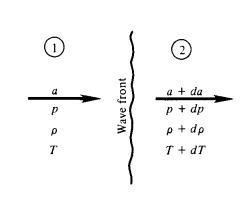
\includegraphics[width=0.3\linewidth]{screenshot001.png}
%	\label{fig:screenshot001}
%\end{figure}
%
By applying a rectangular control volume around this pressure wave, we can apply our conservation equations. We are assuming that these properities are increasing by a small increment. This is why each variable is added by a infinitesimally small term.

Recalling the conservation of mass (continuity equation), $\dot{m} = constant$

\[\dot{m}_{left} = \dot{m}_{right}\]

Recalling he definition of density, $\rho = m/\bar{V}$ and rewriting $\bar{V} = uA$ (check the units)
\[\rho a \cancel{A}  = (\rho + d\rho)(a + da) \cancel{A}\]
Futher expanding gives,
\[\rho a   = (\rho a+ \rho da + a d\rho + da d\rho)\]

We say that $da d\rho$ is so small, we can assume it is zero. This is often referred to as "neglecting higher order terms (H.O.T)". The expression then becomes

\[\frac{da}{a} = -\frac{d \rho}{\rho}\]

For the momentum equation $P + \rho u^2 = constant$
\[P + \rho a^2  = P + dP +  (\rho + d\rho)(a + da)(a + da) \]

But we just said that $\rho a = (\rho + d\rho)(a + da)$


\[P + \rho a^2  = P + dP +  \rho a(a + da) \]
\[dP + \rho ada = a\]

Multiplying the second term by a and divide by a, this is essentially multiplying the second term by one.

\[dP + \rho a^2\frac{da}{a} = a\]

recalling the relation $\frac{da}{a} = -\frac{d \rho}{\rho}$

\[dp - a^2 d \rho = 0\]

                       \[a^2 = \frac{dp}{d\rho}\]

Since a sound wave is a very weak wave, when it travels through a medium, it only increases the pressure and density, etc. slightly. The effect of this is that friction  and heat transfer can be neglected. Since friction cannot be undone, we call this an irreversible process. Whenever there is no transfer of heat, it is called this adiabatic. Thus, the propagation of sound is an adiabatic, reversible process, otherwise called isentropic. Isentropic implies no increase in entropy, which is \textit{not} true in the presence of shock waves.

In the case of a thermally perfect gas, we can say $P = \rho R T$

For a callorically perfect gas we can say $pv^{\gamma} = constant$, where $v$ is volume per unit mass, or specific volume

Differentiating and recalling that $v = 1/\rho$

\[a = \sqrt{\frac{\gamma P}{\rho}} = \sqrt{\gamma R T}\]


\[dm = \left( \rho u\right)_2 - \left(\rho u\right)_1\]
\[D(mV) = \left(\rho u^2 + P \right)_2\]

For Steady flow,

\[\cancel{dm} = \left( \rho u\right)_2 - \left(\rho u\right)_1\]

\[ \left( \rho u\right)_1 = \left(\rho u\right)_2\]

Similarly, for the Momentum equation,

\[\left(\rho u^2 + P\right)_1 = \left(\rho u^2 + P\right)_2\]

Let us change the coordinate system motion for the traveling wave be independent of time, and thus corresponds to \textit{steady state} wave propagation. 
\[ u_1 = \bar{u} + a - \frac{1}{2} \partial u \]
\[ u_2 = \bar{u} + a + \frac{1}{2} \partial u \]


where, $\bar{u}$ is the average flow velocity and $a$ is the wave speed.


Substituting this back into the conservation of mass

\[\left(\rho u\right)_1 = \left(\rho u\right)_2 \]

\[ 
\left( \rho    - \frac{1}{2}\partial \rho \right) 
\left( \bar{u} - a - \frac{1}{2}\partial u\right) = 
\left( \rho    + \frac{1}{2}\partial \rho \right) 
\left( \bar{u} - a + \frac{1}{2}\partial u\right) 
\]

Further expanding

\[
\cancel{
	\rho \bar{u} - \rho a
} + 
\frac{1}{2} 
\left(
-\rho \partial u - \bar{u} - \bar{u} \partial \rho + a \partial \rho 
\right) +
\cancel{
	\frac{1}{4}\partial \rho \partial u 
}
= 
\cancel{
	\rho \bar{u} - \rho a
} + 
\frac{1}{2} 
\left(
\rho \partial u + \bar{u} - \bar{u} \partial \rho - a \partial \rho 
\right) +
\cancel{
	\frac{1}{4}\partial \rho \partial u 
}
\]
 
\[
  \frac{1}{2}\left( - \rho \partial u - \bar{u} \partial \rho + a \partial \rho\right) = 
  \frac{1}{2}\left(   \rho \partial u + \bar{u} \partial \rho - a \partial \rho\right)
\]

\[
\rho \partial u + u \partial \rho - a \partial \rho = 0 
\]

\[
\rho \partial u + \left( u - a\right)\partial \rho = 0
\]

Momentum Equation

\[
\left(\rho u^2 + P\right)_1 = 
\left(\rho u^2 + P\right)_2\]




% \section{Appendix B: Isentropic Waves}

\[dU = dW + dQ\]

For adiabatic, reversible processes, the work done by a system with constant pressure and a change in volume is $-pdV$ and the change in heat energy is zero. Hence,

\[dU = -pdV\].

The change in enthalpy of such a system can be found by taking the derivative of its expression for a thermodynamic process 

\[H = U + pV\]

\[dH = dU + pdV + vdP\]

\[dH = -pdV + pdV + vdP\]

\[dH = vdP\]

The specific heats at constant pressure and constant volume 

\[\left(\frac{\partial U}{\partial T}\right)_v = C_v\]

\[\left(\frac{\partial H}{\partial T}\right)_p = C_p\]

\[\gamma = \frac{C_p}{C_v} = \frac{dH}{dU} = -\frac{VdP}{pdV} = -\frac{V}{dV}\frac{dP}{p}\]

Integrating both sides

\[\gamma \frac{dV}{V} = \frac{-dP}{P} \rightarrow \gamma \int \frac{1}{V} dV = - \int \frac{1}{P} dP\]

\[\gamma ln(V) + ln(P) = C\]

Using log rules

\[ln(V^\gamma) + ln(P) = C\]
 \[ln(pV^\gamma) = C \]
 \[pV^\gamma = e^C = C\]
 
 \[\frac{p}{\rho^\gamma}\]



%--------+----------------------------------------------------------+
%        |  \end{document}                              (REQUIRED)  |
%        |                                                          |
%        |  Details (if you can call them "details") are provided   |
%        |  in section 3.20 of "Read_Me_First_(v12).pdf"            |
%        +----------------------------------------------------------+

\end{document} %---> ---> ---> --->   DO NOT ALTER THIS COMMAND

%XXXXXXXXXXXXXXXXXXXXXXXXXXXXXXXXXXXXXXXXXXXXXXXXXXXXXXXXXXXXXXXXXXXX
%XXXXXXXXXXXXXXXXXXXXXXXXXXXXXXXXXXXXXXXXXXXXXXXXXXXXXXXXXXXXXXXXXXXX
%XXXXXXXXXXXXXXXXXXXXXXXXXXXXXXXXXXXXXXXXXXXXXXXXXXXXXXXXXXXXXXXXXXXX

